\documentclass[twoside]{book}

% Packages required by doxygen
\usepackage{calc}
\usepackage{doxygen}
\usepackage{graphicx}
\usepackage[utf8]{inputenc}
\usepackage{makeidx}
\usepackage{multicol}
\usepackage{multirow}
\usepackage{fixltx2e}
\PassOptionsToPackage{warn}{textcomp}
\usepackage{textcomp}
\usepackage[nointegrals]{wasysym}
\usepackage[table]{xcolor}

% Font selection
\usepackage[T1]{fontenc}
\usepackage{mathptmx}
\usepackage[scaled=.90]{helvet}
\usepackage{courier}
\usepackage{amssymb}
\usepackage{sectsty}
\renewcommand{\familydefault}{\sfdefault}
\allsectionsfont{%
  \fontseries{bc}\selectfont%
  \color{darkgray}%
}
\renewcommand{\DoxyLabelFont}{%
  \fontseries{bc}\selectfont%
  \color{darkgray}%
}
\newcommand{\+}{\discretionary{\mbox{\scriptsize$\hookleftarrow$}}{}{}}

% Page & text layout
\usepackage{geometry}
\geometry{%
  a4paper,%
  top=2.5cm,%
  bottom=2.5cm,%
  left=2.5cm,%
  right=2.5cm%
}
\tolerance=750
\hfuzz=15pt
\hbadness=750
\setlength{\emergencystretch}{15pt}
\setlength{\parindent}{0cm}
\setlength{\parskip}{0.2cm}
\makeatletter
\renewcommand{\paragraph}{%
  \@startsection{paragraph}{4}{0ex}{-1.0ex}{1.0ex}{%
    \normalfont\normalsize\bfseries\SS@parafont%
  }%
}
\renewcommand{\subparagraph}{%
  \@startsection{subparagraph}{5}{0ex}{-1.0ex}{1.0ex}{%
    \normalfont\normalsize\bfseries\SS@subparafont%
  }%
}
\makeatother

% Headers & footers
\usepackage{fancyhdr}
\pagestyle{fancyplain}
\fancyhead[LE]{\fancyplain{}{\bfseries\thepage}}
\fancyhead[CE]{\fancyplain{}{}}
\fancyhead[RE]{\fancyplain{}{\bfseries\leftmark}}
\fancyhead[LO]{\fancyplain{}{\bfseries\rightmark}}
\fancyhead[CO]{\fancyplain{}{}}
\fancyhead[RO]{\fancyplain{}{\bfseries\thepage}}
\fancyfoot[LE]{\fancyplain{}{}}
\fancyfoot[CE]{\fancyplain{}{}}
\fancyfoot[RE]{\fancyplain{}{\bfseries\scriptsize Generated on Sun Feb 8 2015 13\+:14\+:48 for Phd\+Thesis by Doxygen }}
\fancyfoot[LO]{\fancyplain{}{\bfseries\scriptsize Generated on Sun Feb 8 2015 13\+:14\+:48 for Phd\+Thesis by Doxygen }}
\fancyfoot[CO]{\fancyplain{}{}}
\fancyfoot[RO]{\fancyplain{}{}}
\renewcommand{\footrulewidth}{0.4pt}
\renewcommand{\chaptermark}[1]{%
  \markboth{#1}{}%
}
\renewcommand{\sectionmark}[1]{%
  \markright{\thesection\ #1}%
}

% Indices & bibliography
\usepackage{natbib}
\usepackage[titles]{tocloft}
\setcounter{tocdepth}{3}
\setcounter{secnumdepth}{5}
\makeindex

% Hyperlinks (required, but should be loaded last)
\usepackage{ifpdf}
\ifpdf
  \usepackage[pdftex,pagebackref=true]{hyperref}
\else
  \usepackage[ps2pdf,pagebackref=true]{hyperref}
\fi
\hypersetup{%
  colorlinks=true,%
  linkcolor=blue,%
  citecolor=blue,%
  unicode%
}

% Custom commands
\newcommand{\clearemptydoublepage}{%
  \newpage{\pagestyle{empty}\cleardoublepage}%
}


%===== C O N T E N T S =====

\begin{document}

% Titlepage & ToC
\hypersetup{pageanchor=false,
             bookmarks=true,
             bookmarksnumbered=true,
             pdfencoding=unicode
            }
\pagenumbering{roman}
\begin{titlepage}
\vspace*{7cm}
\begin{center}%
{\Large Phd\+Thesis }\\
\vspace*{1cm}
{\large Generated by Doxygen 1.8.7}\\
\vspace*{0.5cm}
{\small Sun Feb 8 2015 13:14:48}\\
\end{center}
\end{titlepage}
\clearemptydoublepage
\tableofcontents
\clearemptydoublepage
\pagenumbering{arabic}
\hypersetup{pageanchor=true}

%--- Begin generated contents ---
\chapter{Namespace Index}
\section{Namespace List}
Here is a list of all namespaces with brief descriptions\+:\begin{DoxyCompactList}
\item\contentsline{section}{\hyperlink{namespacecompute__modularity}{compute\+\_\+modularity} }{\pageref{namespacecompute__modularity}}{}
\item\contentsline{section}{\hyperlink{namespacecv}{cv} }{\pageref{namespacecv}}{}
\end{DoxyCompactList}

\chapter{Hierarchical Index}
\section{Class Hierarchy}
This inheritance list is sorted roughly, but not completely, alphabetically\+:\begin{DoxyCompactList}
\item \contentsline{section}{\+\_\+label}{\pageref{struct__label}}{}
\item \contentsline{section}{Complex\+Network\+Constructor}{\pageref{class_complex_network_constructor}}{}
\item \contentsline{section}{Complex\+Network\+To\+Matlab}{\pageref{class_complex_network_to_matlab}}{}
\item \contentsline{section}{Complex\+Network\+V2$<$ N, E $>$}{\pageref{class_complex_network_v2}}{}
\item \contentsline{section}{Co\+Ocurrence\+Equation}{\pageref{class_co_ocurrence_equation}}{}
\begin{DoxyCompactList}
\item \contentsline{section}{Add\+One\+Co\+Ocurrence\+Equation}{\pageref{class_add_one_co_ocurrence_equation}}{}
\item \contentsline{section}{Reinforcement\+Co\+Ocurrence\+Equation}{\pageref{class_reinforcement_co_ocurrence_equation}}{}
\end{DoxyCompactList}
\item \contentsline{section}{Database\+Reader}{\pageref{class_database_reader}}{}
\begin{DoxyCompactList}
\item \contentsline{section}{K\+Fold\+Database\+Reader\+:\+:Path\+Database\+Reader}{\pageref{class_k_fold_database_reader_1_1_path_database_reader}}{}
\item \contentsline{section}{Sun\+Database\+Reader}{\pageref{class_sun_database_reader}}{}
\end{DoxyCompactList}
\item \contentsline{section}{Complex\+Network\+V2$<$ N, E $>$\+:\+:Edge\+Iterator}{\pageref{class_complex_network_v2_1_1_edge_iterator}}{}
\item \contentsline{section}{Feature\+Abstract}{\pageref{class_feature_abstract}}{}
\begin{DoxyCompactList}
\item \contentsline{section}{Feature$<$ T $>$}{\pageref{class_feature}}{}
\item \contentsline{section}{Feature$<$ float $>$}{\pageref{class_feature}}{}
\begin{DoxyCompactList}
\item \contentsline{section}{Area\+Feature}{\pageref{class_area_feature}}{}
\end{DoxyCompactList}
\item \contentsline{section}{Feature$<$ label $>$}{\pageref{class_feature}}{}
\begin{DoxyCompactList}
\item \contentsline{section}{Label\+Feature}{\pageref{class_label_feature}}{}
\end{DoxyCompactList}
\item \contentsline{section}{Feature$<$ unsigned int $>$}{\pageref{class_feature}}{}
\begin{DoxyCompactList}
\item \contentsline{section}{Orientation\+Feature}{\pageref{class_orientation_feature}}{}
\end{DoxyCompactList}
\end{DoxyCompactList}
\item \contentsline{section}{Feature\+Abstract\+Key}{\pageref{class_feature_abstract_key}}{}
\item \contentsline{section}{Feature\+Abstract\+Ptr}{\pageref{class_feature_abstract_ptr}}{}
\item \contentsline{section}{Feature\+Factory\+Abstract}{\pageref{class_feature_factory_abstract}}{}
\begin{DoxyCompactList}
\item \contentsline{section}{Area\+Feature\+Factory}{\pageref{class_area_feature_factory}}{}
\item \contentsline{section}{Label\+Feature\+Factory}{\pageref{class_label_feature_factory}}{}
\item \contentsline{section}{Orientation\+Feature\+Factory}{\pageref{class_orientation_feature_factory}}{}
\end{DoxyCompactList}
\item \contentsline{section}{get\+Weight}{\pageref{classget_weight}}{}
\item \contentsline{section}{Graph\+Utilities}{\pageref{class_graph_utilities}}{}
\item \contentsline{section}{Features\+Complex\+Network\+:\+:header}{\pageref{struct_features_complex_network_1_1header}}{}
\item \contentsline{section}{Iterative\+Random\+Walk}{\pageref{class_iterative_random_walk}}{}
\item \contentsline{section}{K\+Fold\+Database\+Reader}{\pageref{class_k_fold_database_reader}}{}
\item \contentsline{section}{Label\+Guesser}{\pageref{class_label_guesser}}{}
\item \contentsline{section}{Label\+Guesser\+Experiment}{\pageref{class_label_guesser_experiment}}{}
\item \contentsline{section}{Labels\+Validation\+Experiment}{\pageref{class_labels_validation_experiment}}{}
\item \contentsline{section}{Link}{\pageref{class_link}}{}
\item List\+Digraph\begin{DoxyCompactList}
\item \contentsline{section}{Complex\+Network$<$ N, E $>$}{\pageref{class_complex_network}}{}
\item \contentsline{section}{Complex\+Network$<$ Feature\+Abstract\+Ptr, Link $>$}{\pageref{class_complex_network}}{}
\begin{DoxyCompactList}
\item \contentsline{section}{Features\+Complex\+Network}{\pageref{class_features_complex_network}}{}
\end{DoxyCompactList}
\item \contentsline{section}{Complex\+Network$<$ Node\+String, Link $>$}{\pageref{class_complex_network}}{}
\end{DoxyCompactList}
\item \contentsline{section}{node\+\_\+t}{\pageref{classnode__t}}{}
\item \contentsline{section}{Complex\+Network\+V2$<$ N, E $>$\+:\+:Node\+Iterator}{\pageref{class_complex_network_v2_1_1_node_iterator}}{}
\item \contentsline{section}{Features\+Complex\+Network\+:\+:Node\+Reader}{\pageref{class_features_complex_network_1_1_node_reader}}{}
\item \contentsline{section}{Node\+String}{\pageref{class_node_string}}{}
\item Q\+Label\begin{DoxyCompactList}
\item \contentsline{section}{Supervised\+Image\+Viewer\+Widget}{\pageref{class_supervised_image_viewer_widget}}{}
\end{DoxyCompactList}
\item Q\+Main\+Window\begin{DoxyCompactList}
\item \contentsline{section}{Complex\+Network\+Visualizer}{\pageref{class_complex_network_visualizer}}{}
\end{DoxyCompactList}
\item Q\+Widget\begin{DoxyCompactList}
\item \contentsline{section}{Area\+Feature\+Extraction\+Window}{\pageref{class_area_feature_extraction_window}}{}
\item \contentsline{section}{Complex\+Network\+Viewer\+Widget}{\pageref{class_complex_network_viewer_widget}}{}
\item \contentsline{section}{Database\+Visualizer\+Widget}{\pageref{class_database_visualizer_widget}}{}
\item \contentsline{section}{G\+Main\+Window}{\pageref{class_g_main_window}}{}
\end{DoxyCompactList}
\item \contentsline{section}{Random\+Walk\+Test}{\pageref{class_random_walk_test}}{}
\item \contentsline{section}{Random\+Walk\+Test2}{\pageref{class_random_walk_test2}}{}
\item \contentsline{section}{Region}{\pageref{class_region}}{}
\item \contentsline{section}{Segmenter}{\pageref{class_segmenter}}{}
\item Structure\begin{DoxyCompactList}
\item \contentsline{section}{compute\+\_\+modularity.\+Bt}{\pageref{classcompute__modularity_1_1_bt}}{}
\item \contentsline{section}{compute\+\_\+modularity.\+Edge}{\pageref{classcompute__modularity_1_1_edge}}{}
\item \contentsline{section}{compute\+\_\+modularity.\+Header}{\pageref{classcompute__modularity_1_1_header}}{}
\item \contentsline{section}{compute\+\_\+modularity.\+Label\+Node}{\pageref{classcompute__modularity_1_1_label_node}}{}
\item \contentsline{section}{compute\+\_\+modularity.\+Linka}{\pageref{classcompute__modularity_1_1_linka}}{}
\item \contentsline{section}{compute\+\_\+modularity.\+Node}{\pageref{classcompute__modularity_1_1_node}}{}
\end{DoxyCompactList}
\item \contentsline{section}{S\+U\+N\+Random\+Folder\+Generator}{\pageref{class_s_u_n_random_folder_generator}}{}
\item \contentsline{section}{Supervised\+Image}{\pageref{class_supervised_image}}{}
\end{DoxyCompactList}

\chapter{Class Index}
\section{Class List}
Here are the classes, structs, unions and interfaces with brief descriptions\+:\begin{DoxyCompactList}
\item\contentsline{section}{\hyperlink{class_area_feature_extractor}{Area\+Feature\+Extractor} }{\pageref{class_area_feature_extractor}}{}
\item\contentsline{section}{\hyperlink{class_complex_network}{Complex\+Network$<$ N\+O\+D\+E\+\_\+\+T\+Y\+P\+E, E\+D\+G\+E\+\_\+\+T\+Y\+P\+E $>$} \\*Rede Complexa }{\pageref{class_complex_network}}{}
\item\contentsline{section}{\hyperlink{class_complex_network_constructor}{Complex\+Network\+Constructor} }{\pageref{class_complex_network_constructor}}{}
\item\contentsline{section}{\hyperlink{class_database_reader}{Database\+Reader} }{\pageref{class_database_reader}}{}
\item\contentsline{section}{\hyperlink{class_edge}{Edge$<$ N\+O\+D\+E\+\_\+\+T\+Y\+P\+E, E\+D\+G\+E\+\_\+\+T\+Y\+P\+E $>$} }{\pageref{class_edge}}{}
\item\contentsline{section}{\hyperlink{class_feature}{Feature} }{\pageref{class_feature}}{}
\item\contentsline{section}{\hyperlink{class_feature_extractor}{Feature\+Extractor} }{\pageref{class_feature_extractor}}{}
\item\contentsline{section}{\hyperlink{class_link}{Link} }{\pageref{class_link}}{}
\item\contentsline{section}{\hyperlink{class_node}{Node$<$ N\+O\+D\+E\+\_\+\+T\+Y\+P\+E, E\+D\+G\+E\+\_\+\+T\+Y\+P\+E $>$} }{\pageref{class_node}}{}
\item\contentsline{section}{\hyperlink{classnode__t}{node\+\_\+t} }{\pageref{classnode__t}}{}
\item\contentsline{section}{\hyperlink{class_region}{Region} }{\pageref{class_region}}{}
\item\contentsline{section}{\hyperlink{class_sun_database_reader}{Sun\+Database\+Reader} }{\pageref{class_sun_database_reader}}{}
\item\contentsline{section}{\hyperlink{class_supervised_image}{Supervised\+Image} }{\pageref{class_supervised_image}}{}
\end{DoxyCompactList}

\chapter{File Index}
\section{File List}
Here is a list of all files with brief descriptions\+:\begin{DoxyCompactList}
\item\contentsline{section}{src/\hyperlink{_complex_network_8cpp}{Complex\+Network.\+cpp} }{\pageref{_complex_network_8cpp}}{}
\item\contentsline{section}{src/\hyperlink{_complex_network_8hpp}{Complex\+Network.\+hpp} }{\pageref{_complex_network_8hpp}}{}
\item\contentsline{section}{src/\hyperlink{_edge_8cpp}{Edge.\+cpp} }{\pageref{_edge_8cpp}}{}
\item\contentsline{section}{src/\hyperlink{_edge_8hpp}{Edge.\+hpp} }{\pageref{_edge_8hpp}}{}
\item\contentsline{section}{src/\hyperlink{main_8cpp}{main.\+cpp} }{\pageref{main_8cpp}}{}
\item\contentsline{section}{src/\hyperlink{_node_8cpp}{Node.\+cpp} }{\pageref{_node_8cpp}}{}
\item\contentsline{section}{src/\hyperlink{_node_8hpp}{Node.\+hpp} }{\pageref{_node_8hpp}}{}
\end{DoxyCompactList}

\chapter{Namespace Documentation}
\hypertarget{namespacecompute__modularity}{\section{compute\+\_\+modularity Namespace Reference}
\label{namespacecompute__modularity}\index{compute\+\_\+modularity@{compute\+\_\+modularity}}
}
\subsection*{Classes}
\begin{DoxyCompactItemize}
\item 
class \hyperlink{classcompute__modularity_1_1_bt}{Bt}
\item 
class \hyperlink{classcompute__modularity_1_1_edge}{Edge}
\item 
class \hyperlink{classcompute__modularity_1_1_header}{Header}
\item 
class \hyperlink{classcompute__modularity_1_1_label_node}{Label\+Node}
\item 
class \hyperlink{classcompute__modularity_1_1_linka}{Linka}
\item 
class \hyperlink{classcompute__modularity_1_1_node}{Node}
\end{DoxyCompactItemize}
\subsection*{Functions}
\begin{DoxyCompactItemize}
\item 
def \hyperlink{namespacecompute__modularity_ae7003a81a318f8a965c997e545ed8637}{print\+\_\+all\+\_\+edges}
\item 
def \hyperlink{namespacecompute__modularity_ac8b393251a94473680052f2c0482706e}{read\+\_\+cn\+\_\+file}
\item 
def \hyperlink{namespacecompute__modularity_a607f9b8be1bf581cedf443b517adcf10}{partition}
\item 
def \hyperlink{namespacecompute__modularity_a3dea8443d139544a91b33a28ee635080}{clusters\+Sizes}
\item 
def \hyperlink{namespacecompute__modularity_a632a3219fb7710031adbb61fda6f7b21}{split\+Cluster}
\item 
def \hyperlink{namespacecompute__modularity_aa868b771a28de7a8784a1ac26c141492}{sub\+\_\+clusterization\+\_\+experiment}
\item 
def \hyperlink{namespacecompute__modularity_a3ecf6a23bb6726c84c851283f08dc2c9}{clustering\+\_\+centrallity\+\_\+experiment}
\item 
def \hyperlink{namespacecompute__modularity_ad7008fdd2317a9e3321e23c3518dc2df}{clustering\+\_\+hubs\+\_\+experiment}
\item 
def \hyperlink{namespacecompute__modularity_a03524b2cf695fb83898425ff0f804750}{find\+Node}
\end{DoxyCompactItemize}
\subsection*{Variables}
\begin{DoxyCompactItemize}
\item 
string \hyperlink{namespacecompute__modularity_a9cd9e5b7597978a2a0170d03da499086}{\+\_\+\+\_\+author\+\_\+\+\_\+} = 'wachs'
\item 
tuple \hyperlink{namespacecompute__modularity_abec964e45de0bde923285855ae074cff}{G1} = \hyperlink{namespacecompute__modularity_ac8b393251a94473680052f2c0482706e}{read\+\_\+cn\+\_\+file}('/tmp/Implementation-\/Build/bin/labels\+Network.\+cn')
\item 
tuple \hyperlink{namespacecompute__modularity_ad4ed0b5425c72d4dce599bc986780466}{d} = G1.\+degree()
\end{DoxyCompactItemize}


\subsection{Function Documentation}
\hypertarget{namespacecompute__modularity_a3ecf6a23bb6726c84c851283f08dc2c9}{\index{compute\+\_\+modularity@{compute\+\_\+modularity}!clustering\+\_\+centrallity\+\_\+experiment@{clustering\+\_\+centrallity\+\_\+experiment}}
\index{clustering\+\_\+centrallity\+\_\+experiment@{clustering\+\_\+centrallity\+\_\+experiment}!compute\+\_\+modularity@{compute\+\_\+modularity}}
\subsubsection[{clustering\+\_\+centrallity\+\_\+experiment}]{\setlength{\rightskip}{0pt plus 5cm}def compute\+\_\+modularity.\+clustering\+\_\+centrallity\+\_\+experiment (
\begin{DoxyParamCaption}
\item[{}]{G}
\end{DoxyParamCaption}
)}}\label{namespacecompute__modularity_a3ecf6a23bb6726c84c851283f08dc2c9}


Here is the call graph for this function\+:\nopagebreak
\begin{figure}[H]
\begin{center}
\leavevmode
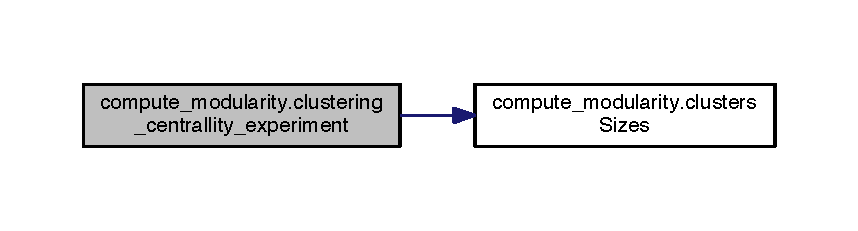
\includegraphics[width=350pt]{namespacecompute__modularity_a3ecf6a23bb6726c84c851283f08dc2c9_cgraph}
\end{center}
\end{figure}


\hypertarget{namespacecompute__modularity_ad7008fdd2317a9e3321e23c3518dc2df}{\index{compute\+\_\+modularity@{compute\+\_\+modularity}!clustering\+\_\+hubs\+\_\+experiment@{clustering\+\_\+hubs\+\_\+experiment}}
\index{clustering\+\_\+hubs\+\_\+experiment@{clustering\+\_\+hubs\+\_\+experiment}!compute\+\_\+modularity@{compute\+\_\+modularity}}
\subsubsection[{clustering\+\_\+hubs\+\_\+experiment}]{\setlength{\rightskip}{0pt plus 5cm}def compute\+\_\+modularity.\+clustering\+\_\+hubs\+\_\+experiment (
\begin{DoxyParamCaption}
\item[{}]{G}
\end{DoxyParamCaption}
)}}\label{namespacecompute__modularity_ad7008fdd2317a9e3321e23c3518dc2df}


Here is the call graph for this function\+:\nopagebreak
\begin{figure}[H]
\begin{center}
\leavevmode
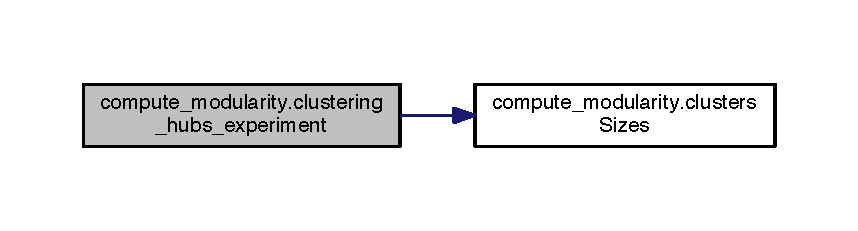
\includegraphics[width=350pt]{namespacecompute__modularity_ad7008fdd2317a9e3321e23c3518dc2df_cgraph}
\end{center}
\end{figure}


\hypertarget{namespacecompute__modularity_a3dea8443d139544a91b33a28ee635080}{\index{compute\+\_\+modularity@{compute\+\_\+modularity}!clusters\+Sizes@{clusters\+Sizes}}
\index{clusters\+Sizes@{clusters\+Sizes}!compute\+\_\+modularity@{compute\+\_\+modularity}}
\subsubsection[{clusters\+Sizes}]{\setlength{\rightskip}{0pt plus 5cm}def compute\+\_\+modularity.\+clusters\+Sizes (
\begin{DoxyParamCaption}
\item[{}]{partition}
\end{DoxyParamCaption}
)}}\label{namespacecompute__modularity_a3dea8443d139544a91b33a28ee635080}


Here is the caller graph for this function\+:\nopagebreak
\begin{figure}[H]
\begin{center}
\leavevmode
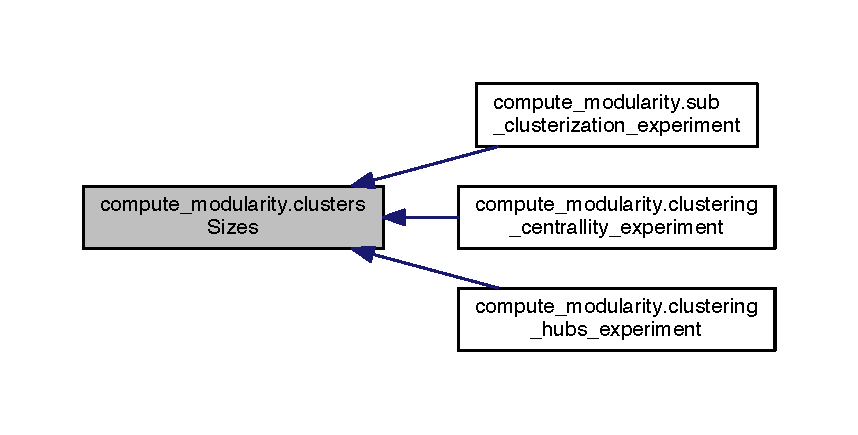
\includegraphics[width=350pt]{namespacecompute__modularity_a3dea8443d139544a91b33a28ee635080_icgraph}
\end{center}
\end{figure}


\hypertarget{namespacecompute__modularity_a03524b2cf695fb83898425ff0f804750}{\index{compute\+\_\+modularity@{compute\+\_\+modularity}!find\+Node@{find\+Node}}
\index{find\+Node@{find\+Node}!compute\+\_\+modularity@{compute\+\_\+modularity}}
\subsubsection[{find\+Node}]{\setlength{\rightskip}{0pt plus 5cm}def compute\+\_\+modularity.\+find\+Node (
\begin{DoxyParamCaption}
\item[{}]{G, }
\item[{}]{text}
\end{DoxyParamCaption}
)}}\label{namespacecompute__modularity_a03524b2cf695fb83898425ff0f804750}


Here is the caller graph for this function\+:\nopagebreak
\begin{figure}[H]
\begin{center}
\leavevmode
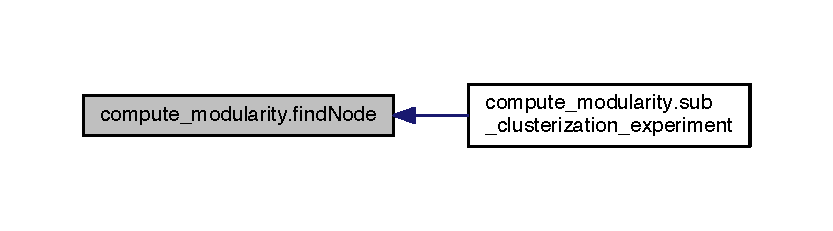
\includegraphics[width=350pt]{namespacecompute__modularity_a03524b2cf695fb83898425ff0f804750_icgraph}
\end{center}
\end{figure}


\hypertarget{namespacecompute__modularity_a607f9b8be1bf581cedf443b517adcf10}{\index{compute\+\_\+modularity@{compute\+\_\+modularity}!partition@{partition}}
\index{partition@{partition}!compute\+\_\+modularity@{compute\+\_\+modularity}}
\subsubsection[{partition}]{\setlength{\rightskip}{0pt plus 5cm}def compute\+\_\+modularity.\+partition (
\begin{DoxyParamCaption}
\item[{}]{G}
\end{DoxyParamCaption}
)}}\label{namespacecompute__modularity_a607f9b8be1bf581cedf443b517adcf10}


Here is the caller graph for this function\+:\nopagebreak
\begin{figure}[H]
\begin{center}
\leavevmode
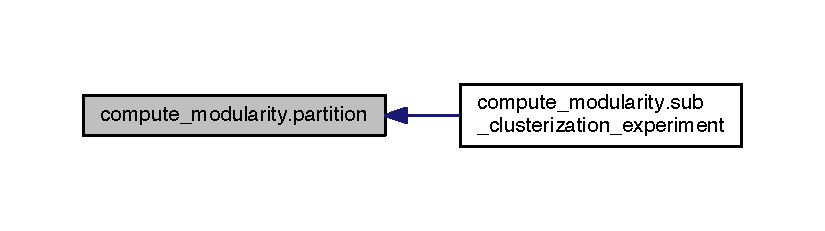
\includegraphics[width=350pt]{namespacecompute__modularity_a607f9b8be1bf581cedf443b517adcf10_icgraph}
\end{center}
\end{figure}


\hypertarget{namespacecompute__modularity_ae7003a81a318f8a965c997e545ed8637}{\index{compute\+\_\+modularity@{compute\+\_\+modularity}!print\+\_\+all\+\_\+edges@{print\+\_\+all\+\_\+edges}}
\index{print\+\_\+all\+\_\+edges@{print\+\_\+all\+\_\+edges}!compute\+\_\+modularity@{compute\+\_\+modularity}}
\subsubsection[{print\+\_\+all\+\_\+edges}]{\setlength{\rightskip}{0pt plus 5cm}def compute\+\_\+modularity.\+print\+\_\+all\+\_\+edges (
\begin{DoxyParamCaption}
\item[{}]{G}
\end{DoxyParamCaption}
)}}\label{namespacecompute__modularity_ae7003a81a318f8a965c997e545ed8637}
\hypertarget{namespacecompute__modularity_ac8b393251a94473680052f2c0482706e}{\index{compute\+\_\+modularity@{compute\+\_\+modularity}!read\+\_\+cn\+\_\+file@{read\+\_\+cn\+\_\+file}}
\index{read\+\_\+cn\+\_\+file@{read\+\_\+cn\+\_\+file}!compute\+\_\+modularity@{compute\+\_\+modularity}}
\subsubsection[{read\+\_\+cn\+\_\+file}]{\setlength{\rightskip}{0pt plus 5cm}def compute\+\_\+modularity.\+read\+\_\+cn\+\_\+file (
\begin{DoxyParamCaption}
\item[{}]{path}
\end{DoxyParamCaption}
)}}\label{namespacecompute__modularity_ac8b393251a94473680052f2c0482706e}
\hypertarget{namespacecompute__modularity_a632a3219fb7710031adbb61fda6f7b21}{\index{compute\+\_\+modularity@{compute\+\_\+modularity}!split\+Cluster@{split\+Cluster}}
\index{split\+Cluster@{split\+Cluster}!compute\+\_\+modularity@{compute\+\_\+modularity}}
\subsubsection[{split\+Cluster}]{\setlength{\rightskip}{0pt plus 5cm}def compute\+\_\+modularity.\+split\+Cluster (
\begin{DoxyParamCaption}
\item[{}]{G, }
\item[{}]{partition, }
\item[{}]{x}
\end{DoxyParamCaption}
)}}\label{namespacecompute__modularity_a632a3219fb7710031adbb61fda6f7b21}


Here is the caller graph for this function\+:\nopagebreak
\begin{figure}[H]
\begin{center}
\leavevmode
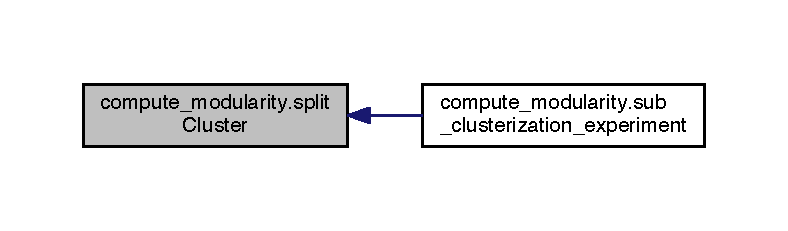
\includegraphics[width=350pt]{namespacecompute__modularity_a632a3219fb7710031adbb61fda6f7b21_icgraph}
\end{center}
\end{figure}


\hypertarget{namespacecompute__modularity_aa868b771a28de7a8784a1ac26c141492}{\index{compute\+\_\+modularity@{compute\+\_\+modularity}!sub\+\_\+clusterization\+\_\+experiment@{sub\+\_\+clusterization\+\_\+experiment}}
\index{sub\+\_\+clusterization\+\_\+experiment@{sub\+\_\+clusterization\+\_\+experiment}!compute\+\_\+modularity@{compute\+\_\+modularity}}
\subsubsection[{sub\+\_\+clusterization\+\_\+experiment}]{\setlength{\rightskip}{0pt plus 5cm}def compute\+\_\+modularity.\+sub\+\_\+clusterization\+\_\+experiment (
\begin{DoxyParamCaption}
\item[{}]{G1}
\end{DoxyParamCaption}
)}}\label{namespacecompute__modularity_aa868b771a28de7a8784a1ac26c141492}


Here is the call graph for this function\+:\nopagebreak
\begin{figure}[H]
\begin{center}
\leavevmode
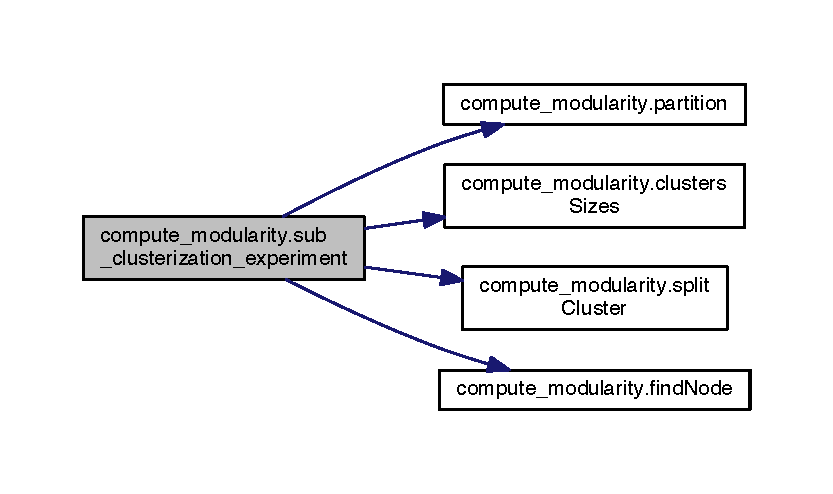
\includegraphics[width=350pt]{namespacecompute__modularity_aa868b771a28de7a8784a1ac26c141492_cgraph}
\end{center}
\end{figure}




\subsection{Variable Documentation}
\hypertarget{namespacecompute__modularity_a9cd9e5b7597978a2a0170d03da499086}{\index{compute\+\_\+modularity@{compute\+\_\+modularity}!\+\_\+\+\_\+author\+\_\+\+\_\+@{\+\_\+\+\_\+author\+\_\+\+\_\+}}
\index{\+\_\+\+\_\+author\+\_\+\+\_\+@{\+\_\+\+\_\+author\+\_\+\+\_\+}!compute\+\_\+modularity@{compute\+\_\+modularity}}
\subsubsection[{\+\_\+\+\_\+author\+\_\+\+\_\+}]{\setlength{\rightskip}{0pt plus 5cm}string compute\+\_\+modularity.\+\_\+\+\_\+author\+\_\+\+\_\+ = 'wachs'}}\label{namespacecompute__modularity_a9cd9e5b7597978a2a0170d03da499086}
\hypertarget{namespacecompute__modularity_ad4ed0b5425c72d4dce599bc986780466}{\index{compute\+\_\+modularity@{compute\+\_\+modularity}!d@{d}}
\index{d@{d}!compute\+\_\+modularity@{compute\+\_\+modularity}}
\subsubsection[{d}]{\setlength{\rightskip}{0pt plus 5cm}tuple compute\+\_\+modularity.\+d = G1.\+degree()}}\label{namespacecompute__modularity_ad4ed0b5425c72d4dce599bc986780466}
\hypertarget{namespacecompute__modularity_abec964e45de0bde923285855ae074cff}{\index{compute\+\_\+modularity@{compute\+\_\+modularity}!G1@{G1}}
\index{G1@{G1}!compute\+\_\+modularity@{compute\+\_\+modularity}}
\subsubsection[{G1}]{\setlength{\rightskip}{0pt plus 5cm}tuple compute\+\_\+modularity.\+G1 = {\bf read\+\_\+cn\+\_\+file}('/tmp/Implementation-\/Build/bin/labels\+Network.\+cn')}}\label{namespacecompute__modularity_abec964e45de0bde923285855ae074cff}

\chapter{Class Documentation}
\hypertarget{struct__label}{\section{\+\_\+label Struct Reference}
\label{struct__label}\index{\+\_\+label@{\+\_\+label}}
}


{\ttfamily \#include $<$Label\+Feature.\+hpp$>$}

\subsection*{Public Member Functions}
\begin{DoxyCompactItemize}
\item 
\hyperlink{struct__label_ade65765434ea6e97ad4bdecf70dc2505}{\+\_\+label} ()
\item 
\hyperlink{struct__label_afe885787cc58bb203aa2e0c1a1e9770b}{\+\_\+label} (const char $\ast$val)
\end{DoxyCompactItemize}
\subsection*{Public Attributes}
\begin{DoxyCompactItemize}
\item 
char \hyperlink{struct__label_aa7154ad6c9bb58841aefe2a29bcaa940}{value} \mbox{[}50\mbox{]}
\end{DoxyCompactItemize}


Collaboration diagram for \+\_\+label\+:\nopagebreak
\begin{figure}[H]
\begin{center}
\leavevmode
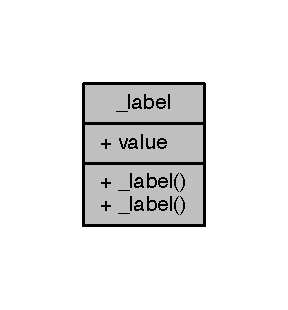
\includegraphics[width=138pt]{struct__label__coll__graph}
\end{center}
\end{figure}


\subsection{Constructor \& Destructor Documentation}
\hypertarget{struct__label_ade65765434ea6e97ad4bdecf70dc2505}{\index{\+\_\+label@{\+\_\+label}!\+\_\+label@{\+\_\+label}}
\index{\+\_\+label@{\+\_\+label}!\+\_\+label@{\+\_\+label}}
\subsubsection[{\+\_\+label}]{\setlength{\rightskip}{0pt plus 5cm}\+\_\+label\+::\+\_\+label (
\begin{DoxyParamCaption}
{}
\end{DoxyParamCaption}
)\hspace{0.3cm}{\ttfamily [inline]}}}\label{struct__label_ade65765434ea6e97ad4bdecf70dc2505}
\hypertarget{struct__label_afe885787cc58bb203aa2e0c1a1e9770b}{\index{\+\_\+label@{\+\_\+label}!\+\_\+label@{\+\_\+label}}
\index{\+\_\+label@{\+\_\+label}!\+\_\+label@{\+\_\+label}}
\subsubsection[{\+\_\+label}]{\setlength{\rightskip}{0pt plus 5cm}\+\_\+label\+::\+\_\+label (
\begin{DoxyParamCaption}
\item[{const char $\ast$}]{val}
\end{DoxyParamCaption}
)\hspace{0.3cm}{\ttfamily [inline]}}}\label{struct__label_afe885787cc58bb203aa2e0c1a1e9770b}


\subsection{Member Data Documentation}
\hypertarget{struct__label_aa7154ad6c9bb58841aefe2a29bcaa940}{\index{\+\_\+label@{\+\_\+label}!value@{value}}
\index{value@{value}!\+\_\+label@{\+\_\+label}}
\subsubsection[{value}]{\setlength{\rightskip}{0pt plus 5cm}char \+\_\+label\+::value\mbox{[}50\mbox{]}}}\label{struct__label_aa7154ad6c9bb58841aefe2a29bcaa940}


The documentation for this struct was generated from the following file\+:\begin{DoxyCompactItemize}
\item 
Sources/\+Feature\+Extractors/\hyperlink{_label_feature_8hpp}{Label\+Feature.\+hpp}\end{DoxyCompactItemize}

\hypertarget{class_area_feature}{\section{Area\+Feature Class Reference}
\label{class_area_feature}\index{Area\+Feature@{Area\+Feature}}
}


{\ttfamily \#include $<$Area\+Feature.\+hpp$>$}

\subsection*{Public Member Functions}
\begin{DoxyCompactItemize}
\item 
\hyperlink{class_area_feature_af65d43c5c868babfb6c429464f36a898}{Area\+Feature} (float value)
\item 
const char $\ast$ \hyperlink{class_area_feature_a6c0a6e3346ba2ddaa4a50cb957f08ab2}{as\+String} (char $\ast$buffer) const 
\item 
void \hyperlink{class_area_feature_ac0edad4aaa2a45caabd27112017bf4a6}{Write\+To\+Stream} (std\+::ostream \&stream) const 
\end{DoxyCompactItemize}
\subsection*{Friends}
\begin{DoxyCompactItemize}
\item 
class \hyperlink{class_area_feature_acf274ff5848a30a105c61f0e1c56cf7e}{Area\+Feature\+Factory}
\end{DoxyCompactItemize}
\subsection*{Additional Inherited Members}


Inheritance diagram for Area\+Feature\+:
\nopagebreak
\begin{figure}[H]
\begin{center}
\leavevmode
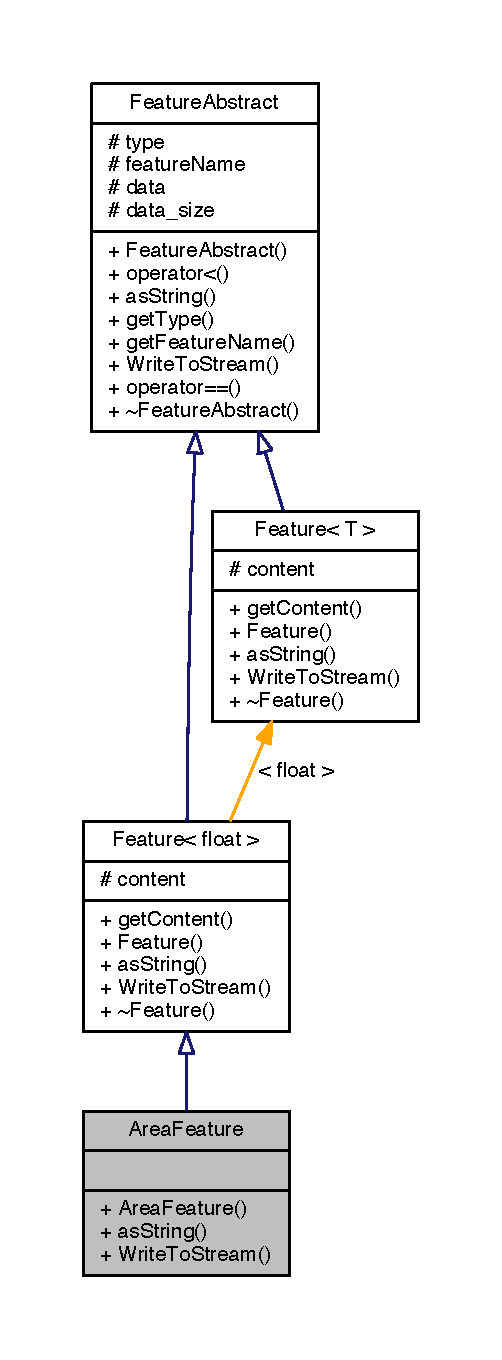
\includegraphics[height=550pt]{class_area_feature__inherit__graph}
\end{center}
\end{figure}


Collaboration diagram for Area\+Feature\+:
\nopagebreak
\begin{figure}[H]
\begin{center}
\leavevmode
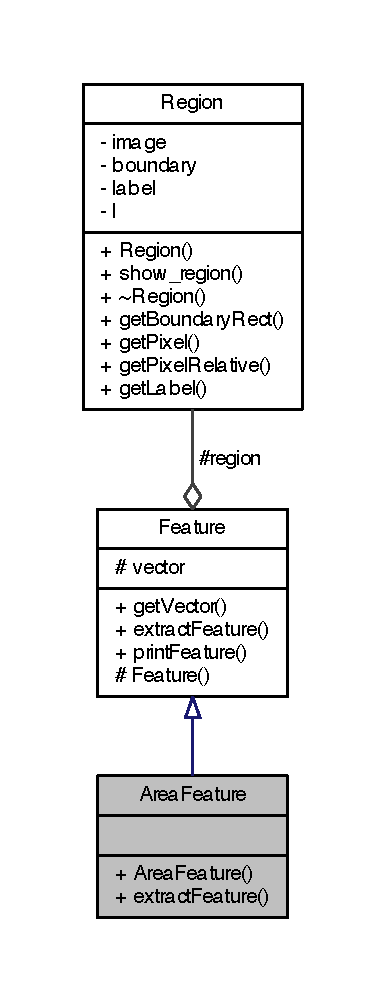
\includegraphics[height=550pt]{class_area_feature__coll__graph}
\end{center}
\end{figure}


\subsection{Constructor \& Destructor Documentation}
\hypertarget{class_area_feature_af65d43c5c868babfb6c429464f36a898}{\index{Area\+Feature@{Area\+Feature}!Area\+Feature@{Area\+Feature}}
\index{Area\+Feature@{Area\+Feature}!Area\+Feature@{Area\+Feature}}
\subsubsection[{Area\+Feature}]{\setlength{\rightskip}{0pt plus 5cm}Area\+Feature\+::\+Area\+Feature (
\begin{DoxyParamCaption}
\item[{float}]{value}
\end{DoxyParamCaption}
)}}\label{class_area_feature_af65d43c5c868babfb6c429464f36a898}


\subsection{Member Function Documentation}
\hypertarget{class_area_feature_a6c0a6e3346ba2ddaa4a50cb957f08ab2}{\index{Area\+Feature@{Area\+Feature}!as\+String@{as\+String}}
\index{as\+String@{as\+String}!Area\+Feature@{Area\+Feature}}
\subsubsection[{as\+String}]{\setlength{\rightskip}{0pt plus 5cm}const char $\ast$ Area\+Feature\+::as\+String (
\begin{DoxyParamCaption}
\item[{char $\ast$}]{buffer}
\end{DoxyParamCaption}
) const\hspace{0.3cm}{\ttfamily [virtual]}}}\label{class_area_feature_a6c0a6e3346ba2ddaa4a50cb957f08ab2}


Implements \hyperlink{class_feature_abdd71dfec0efebf4ff17aeb2bee257c3}{Feature$<$ float $>$}.

\hypertarget{class_area_feature_ac0edad4aaa2a45caabd27112017bf4a6}{\index{Area\+Feature@{Area\+Feature}!Write\+To\+Stream@{Write\+To\+Stream}}
\index{Write\+To\+Stream@{Write\+To\+Stream}!Area\+Feature@{Area\+Feature}}
\subsubsection[{Write\+To\+Stream}]{\setlength{\rightskip}{0pt plus 5cm}void Area\+Feature\+::\+Write\+To\+Stream (
\begin{DoxyParamCaption}
\item[{std\+::ostream \&}]{stream}
\end{DoxyParamCaption}
) const\hspace{0.3cm}{\ttfamily [virtual]}}}\label{class_area_feature_ac0edad4aaa2a45caabd27112017bf4a6}


Implements \hyperlink{class_feature_a459aef7873c75fb23ede86f71361239b}{Feature$<$ float $>$}.



\subsection{Friends And Related Function Documentation}
\hypertarget{class_area_feature_acf274ff5848a30a105c61f0e1c56cf7e}{\index{Area\+Feature@{Area\+Feature}!Area\+Feature\+Factory@{Area\+Feature\+Factory}}
\index{Area\+Feature\+Factory@{Area\+Feature\+Factory}!Area\+Feature@{Area\+Feature}}
\subsubsection[{Area\+Feature\+Factory}]{\setlength{\rightskip}{0pt plus 5cm}friend class {\bf Area\+Feature\+Factory}\hspace{0.3cm}{\ttfamily [friend]}}}\label{class_area_feature_acf274ff5848a30a105c61f0e1c56cf7e}


The documentation for this class was generated from the following files\+:\begin{DoxyCompactItemize}
\item 
Sources/\+Feature\+Extractors/\hyperlink{_area_feature_8hpp}{Area\+Feature.\+hpp}\item 
Sources/\+Feature\+Extractors/\hyperlink{_area_feature_8cpp}{Area\+Feature.\+cpp}\end{DoxyCompactItemize}

\hypertarget{class_area_feature_extraction_window}{\section{Area\+Feature\+Extraction\+Window Class Reference}
\label{class_area_feature_extraction_window}\index{Area\+Feature\+Extraction\+Window@{Area\+Feature\+Extraction\+Window}}
}


{\ttfamily \#include $<$Area\+Feature\+Extraction\+Window.\+hpp$>$}

\subsection*{Public Slots}
\begin{DoxyCompactItemize}
\item 
void \hyperlink{class_area_feature_extraction_window_aa478c08abe712412d90fa48936c05fa1}{show\+\_\+next} ()
\item 
void \hyperlink{class_area_feature_extraction_window_ab0f1fc10645d98e916faea9a94cf2a15}{show\+\_\+previous} ()
\end{DoxyCompactItemize}
\subsection*{Public Member Functions}
\begin{DoxyCompactItemize}
\item 
\hyperlink{class_area_feature_extraction_window_abcf541b8a70c5122524facefd7fc3f4b}{Area\+Feature\+Extraction\+Window} (Q\+String database\+Path, Q\+Widget $\ast$parent=0)
\end{DoxyCompactItemize}
\subsection*{Private Attributes}
\begin{DoxyCompactItemize}
\item 
Q\+Push\+Button $\ast$ \hyperlink{class_area_feature_extraction_window_aeac146ce4d4824383ae3387200771c8c}{m\+\_\+next\+\_\+button}
\item 
Q\+Push\+Button $\ast$ \hyperlink{class_area_feature_extraction_window_af79c0e607fea8013225fdd1142fba23a}{m\+\_\+previous\+\_\+button}
\item 
Q\+V\+Box\+Layout $\ast$ \hyperlink{class_area_feature_extraction_window_ab76bcfe16b8e327f97114dd56787eaec}{m\+\_\+vbox}
\item 
Q\+H\+Box\+Layout $\ast$ \hyperlink{class_area_feature_extraction_window_a5664dd1b2be2c4726cc016ced8828fc3}{m\+\_\+hbox}
\item 
\hyperlink{class_supervised_image_viewer_widget}{Supervised\+Image\+Viewer\+Widget} $\ast$ \hyperlink{class_area_feature_extraction_window_a5e92f22f7471682136650c210abb34d3}{m\+\_\+supervised\+Widget}
\item 
\hyperlink{class_sun_database_reader}{Sun\+Database\+Reader} \hyperlink{class_area_feature_extraction_window_a428a7715193feb571ec8ba70fe55fc4d}{reader}
\end{DoxyCompactItemize}


Inheritance diagram for Area\+Feature\+Extraction\+Window\+:\nopagebreak
\begin{figure}[H]
\begin{center}
\leavevmode
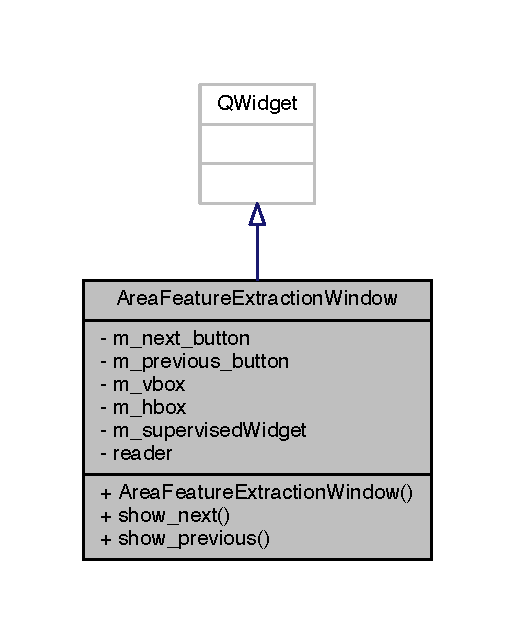
\includegraphics[width=247pt]{class_area_feature_extraction_window__inherit__graph}
\end{center}
\end{figure}


Collaboration diagram for Area\+Feature\+Extraction\+Window\+:
\nopagebreak
\begin{figure}[H]
\begin{center}
\leavevmode
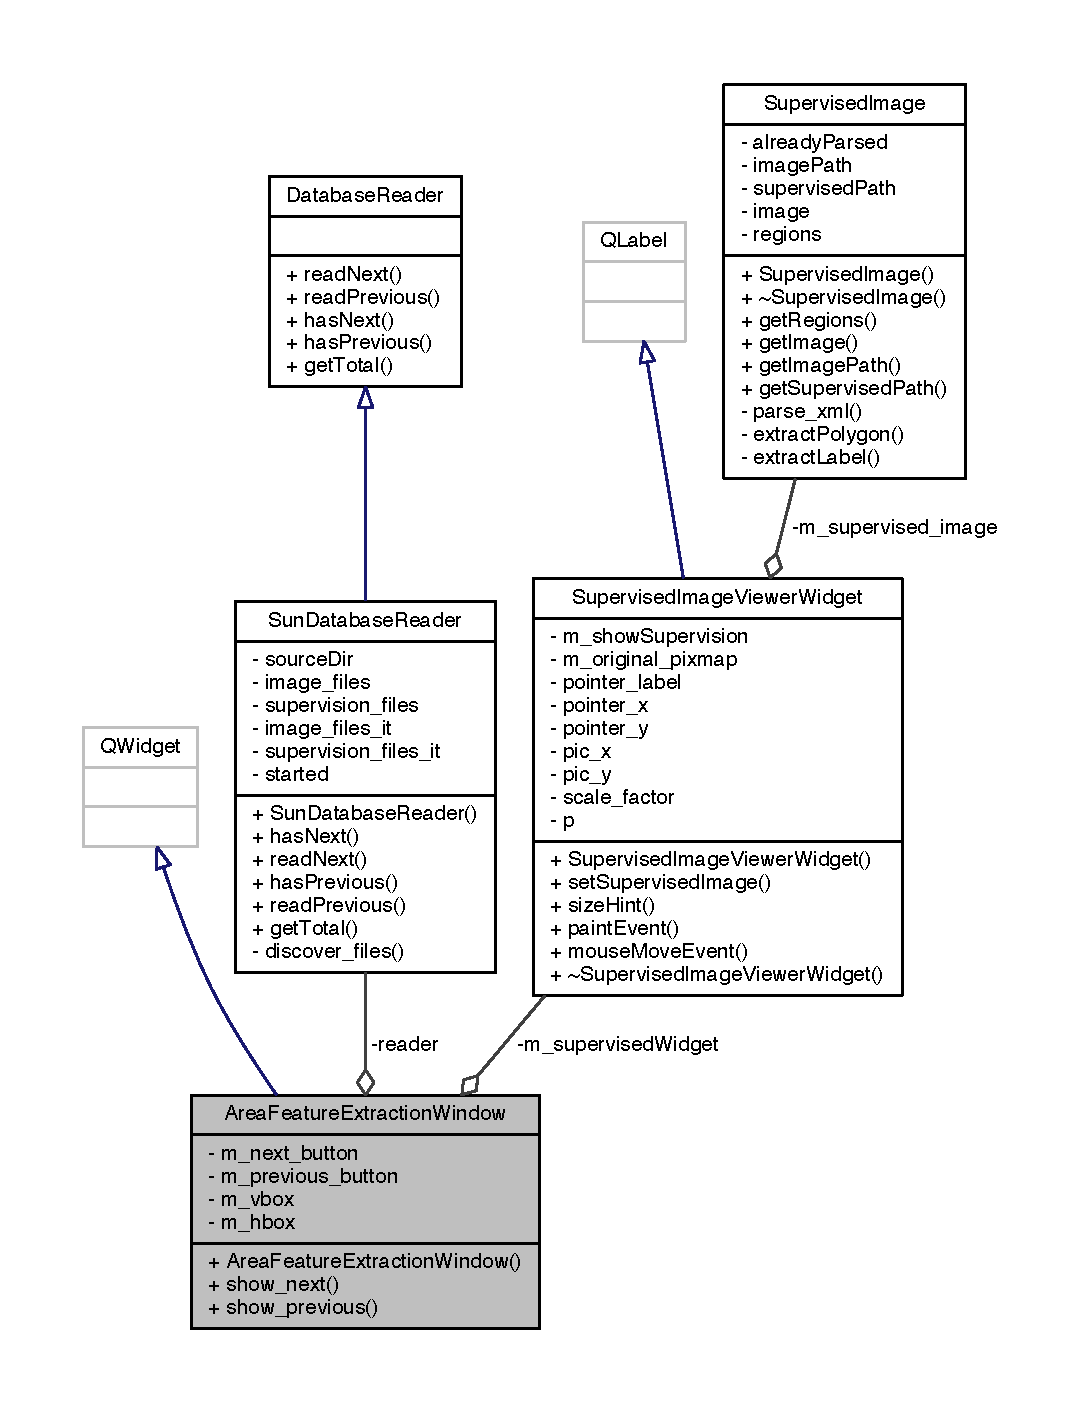
\includegraphics[width=350pt]{class_area_feature_extraction_window__coll__graph}
\end{center}
\end{figure}


\subsection{Constructor \& Destructor Documentation}
\hypertarget{class_area_feature_extraction_window_abcf541b8a70c5122524facefd7fc3f4b}{\index{Area\+Feature\+Extraction\+Window@{Area\+Feature\+Extraction\+Window}!Area\+Feature\+Extraction\+Window@{Area\+Feature\+Extraction\+Window}}
\index{Area\+Feature\+Extraction\+Window@{Area\+Feature\+Extraction\+Window}!Area\+Feature\+Extraction\+Window@{Area\+Feature\+Extraction\+Window}}
\subsubsection[{Area\+Feature\+Extraction\+Window}]{\setlength{\rightskip}{0pt plus 5cm}Area\+Feature\+Extraction\+Window\+::\+Area\+Feature\+Extraction\+Window (
\begin{DoxyParamCaption}
\item[{Q\+String}]{database\+Path, }
\item[{Q\+Widget $\ast$}]{parent = {\ttfamily 0}}
\end{DoxyParamCaption}
)\hspace{0.3cm}{\ttfamily [explicit]}}}\label{class_area_feature_extraction_window_abcf541b8a70c5122524facefd7fc3f4b}


Here is the call graph for this function\+:
\nopagebreak
\begin{figure}[H]
\begin{center}
\leavevmode
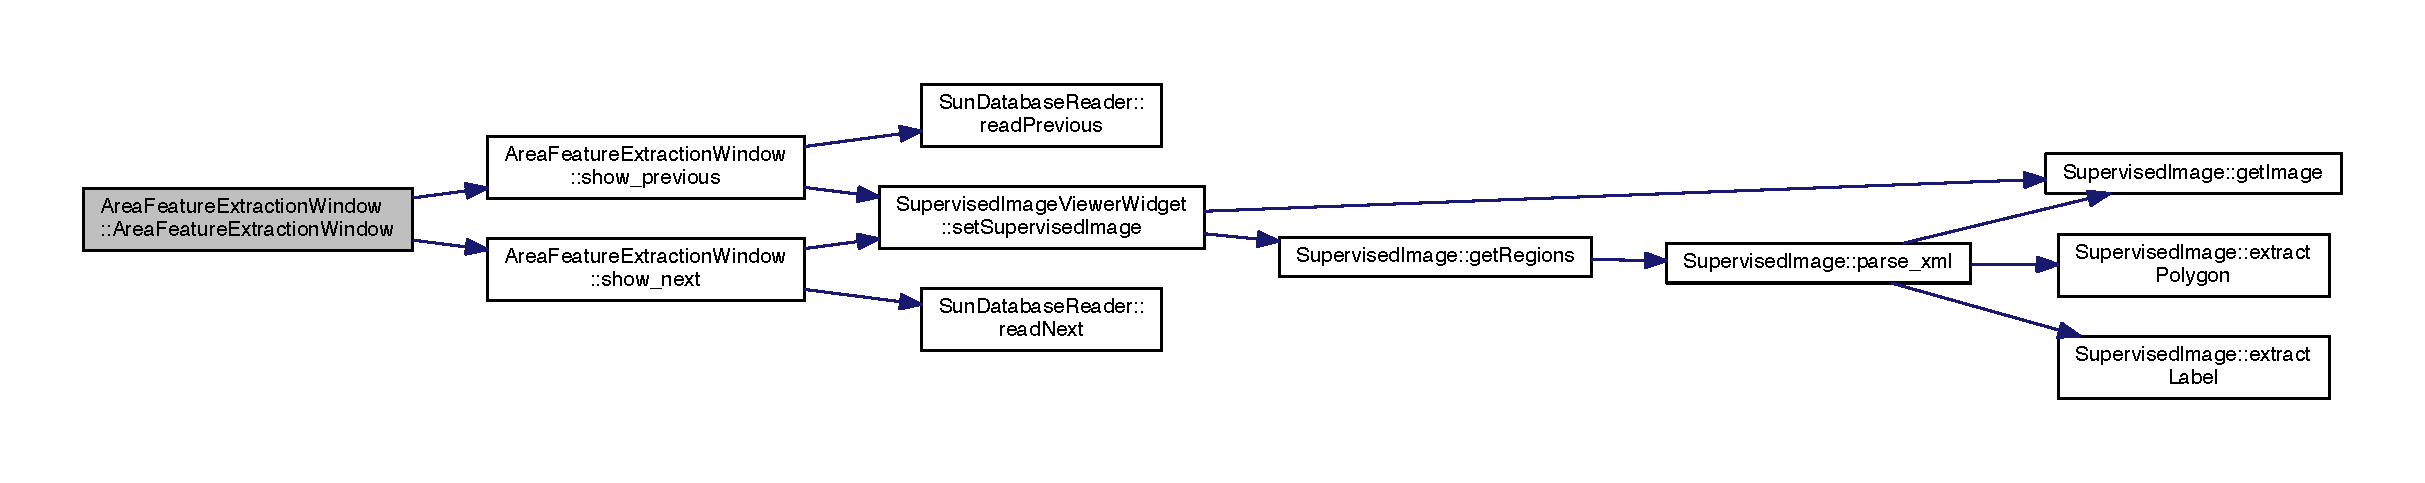
\includegraphics[width=350pt]{class_area_feature_extraction_window_abcf541b8a70c5122524facefd7fc3f4b_cgraph}
\end{center}
\end{figure}




\subsection{Member Function Documentation}
\hypertarget{class_area_feature_extraction_window_aa478c08abe712412d90fa48936c05fa1}{\index{Area\+Feature\+Extraction\+Window@{Area\+Feature\+Extraction\+Window}!show\+\_\+next@{show\+\_\+next}}
\index{show\+\_\+next@{show\+\_\+next}!Area\+Feature\+Extraction\+Window@{Area\+Feature\+Extraction\+Window}}
\subsubsection[{show\+\_\+next}]{\setlength{\rightskip}{0pt plus 5cm}void Area\+Feature\+Extraction\+Window\+::show\+\_\+next (
\begin{DoxyParamCaption}
{}
\end{DoxyParamCaption}
)\hspace{0.3cm}{\ttfamily [slot]}}}\label{class_area_feature_extraction_window_aa478c08abe712412d90fa48936c05fa1}


Here is the call graph for this function\+:
\nopagebreak
\begin{figure}[H]
\begin{center}
\leavevmode
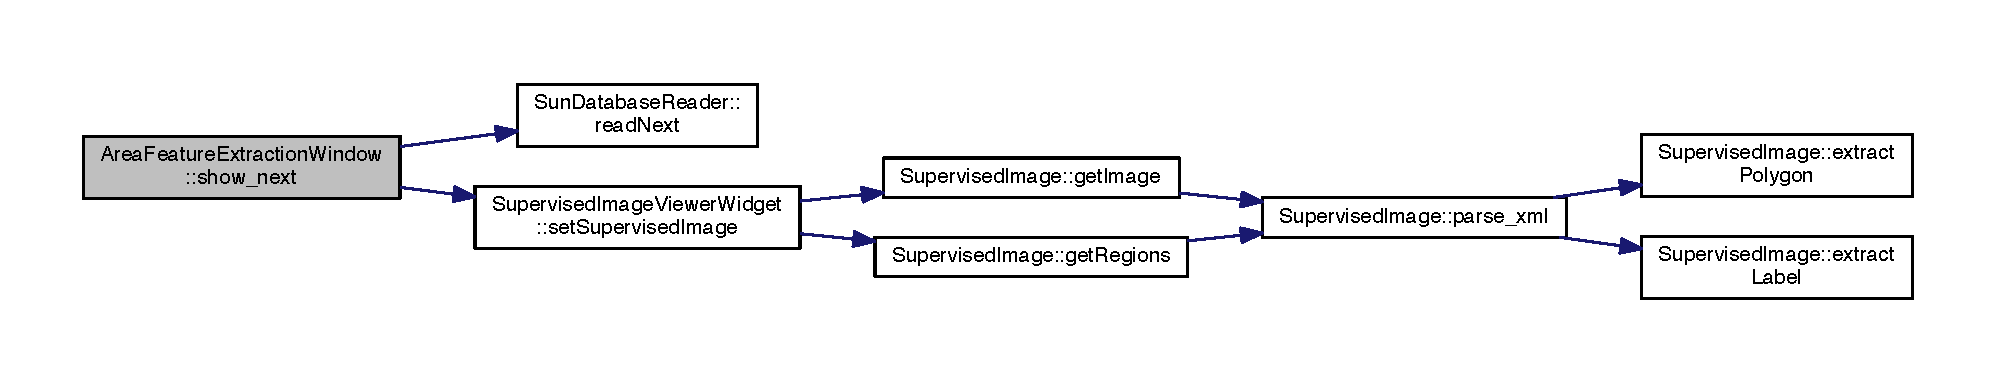
\includegraphics[width=350pt]{class_area_feature_extraction_window_aa478c08abe712412d90fa48936c05fa1_cgraph}
\end{center}
\end{figure}




Here is the caller graph for this function\+:\nopagebreak
\begin{figure}[H]
\begin{center}
\leavevmode
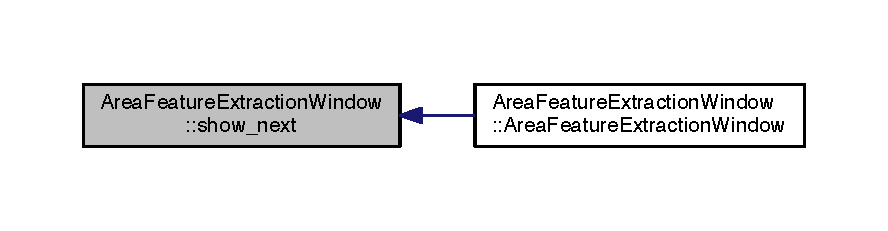
\includegraphics[width=350pt]{class_area_feature_extraction_window_aa478c08abe712412d90fa48936c05fa1_icgraph}
\end{center}
\end{figure}


\hypertarget{class_area_feature_extraction_window_ab0f1fc10645d98e916faea9a94cf2a15}{\index{Area\+Feature\+Extraction\+Window@{Area\+Feature\+Extraction\+Window}!show\+\_\+previous@{show\+\_\+previous}}
\index{show\+\_\+previous@{show\+\_\+previous}!Area\+Feature\+Extraction\+Window@{Area\+Feature\+Extraction\+Window}}
\subsubsection[{show\+\_\+previous}]{\setlength{\rightskip}{0pt plus 5cm}void Area\+Feature\+Extraction\+Window\+::show\+\_\+previous (
\begin{DoxyParamCaption}
{}
\end{DoxyParamCaption}
)\hspace{0.3cm}{\ttfamily [slot]}}}\label{class_area_feature_extraction_window_ab0f1fc10645d98e916faea9a94cf2a15}


Here is the call graph for this function\+:
\nopagebreak
\begin{figure}[H]
\begin{center}
\leavevmode
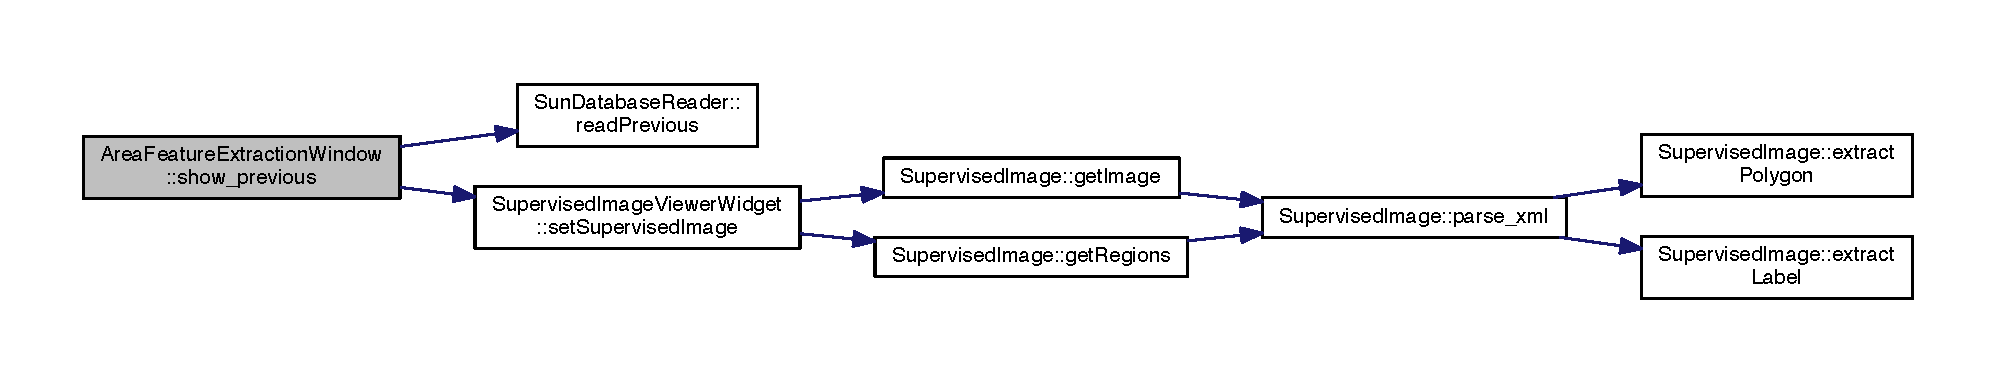
\includegraphics[width=350pt]{class_area_feature_extraction_window_ab0f1fc10645d98e916faea9a94cf2a15_cgraph}
\end{center}
\end{figure}




Here is the caller graph for this function\+:\nopagebreak
\begin{figure}[H]
\begin{center}
\leavevmode
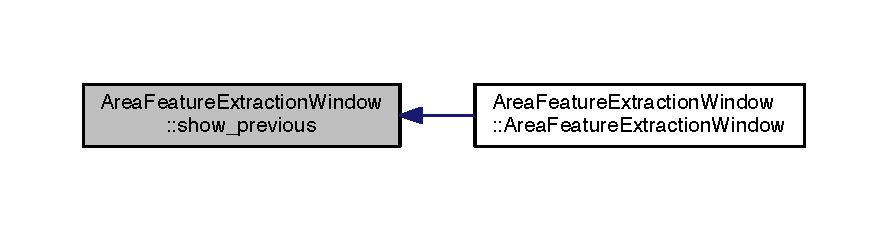
\includegraphics[width=350pt]{class_area_feature_extraction_window_ab0f1fc10645d98e916faea9a94cf2a15_icgraph}
\end{center}
\end{figure}




\subsection{Member Data Documentation}
\hypertarget{class_area_feature_extraction_window_a5664dd1b2be2c4726cc016ced8828fc3}{\index{Area\+Feature\+Extraction\+Window@{Area\+Feature\+Extraction\+Window}!m\+\_\+hbox@{m\+\_\+hbox}}
\index{m\+\_\+hbox@{m\+\_\+hbox}!Area\+Feature\+Extraction\+Window@{Area\+Feature\+Extraction\+Window}}
\subsubsection[{m\+\_\+hbox}]{\setlength{\rightskip}{0pt plus 5cm}Q\+H\+Box\+Layout$\ast$ Area\+Feature\+Extraction\+Window\+::m\+\_\+hbox\hspace{0.3cm}{\ttfamily [private]}}}\label{class_area_feature_extraction_window_a5664dd1b2be2c4726cc016ced8828fc3}
\hypertarget{class_area_feature_extraction_window_aeac146ce4d4824383ae3387200771c8c}{\index{Area\+Feature\+Extraction\+Window@{Area\+Feature\+Extraction\+Window}!m\+\_\+next\+\_\+button@{m\+\_\+next\+\_\+button}}
\index{m\+\_\+next\+\_\+button@{m\+\_\+next\+\_\+button}!Area\+Feature\+Extraction\+Window@{Area\+Feature\+Extraction\+Window}}
\subsubsection[{m\+\_\+next\+\_\+button}]{\setlength{\rightskip}{0pt plus 5cm}Q\+Push\+Button$\ast$ Area\+Feature\+Extraction\+Window\+::m\+\_\+next\+\_\+button\hspace{0.3cm}{\ttfamily [private]}}}\label{class_area_feature_extraction_window_aeac146ce4d4824383ae3387200771c8c}
\hypertarget{class_area_feature_extraction_window_af79c0e607fea8013225fdd1142fba23a}{\index{Area\+Feature\+Extraction\+Window@{Area\+Feature\+Extraction\+Window}!m\+\_\+previous\+\_\+button@{m\+\_\+previous\+\_\+button}}
\index{m\+\_\+previous\+\_\+button@{m\+\_\+previous\+\_\+button}!Area\+Feature\+Extraction\+Window@{Area\+Feature\+Extraction\+Window}}
\subsubsection[{m\+\_\+previous\+\_\+button}]{\setlength{\rightskip}{0pt plus 5cm}Q\+Push\+Button$\ast$ Area\+Feature\+Extraction\+Window\+::m\+\_\+previous\+\_\+button\hspace{0.3cm}{\ttfamily [private]}}}\label{class_area_feature_extraction_window_af79c0e607fea8013225fdd1142fba23a}
\hypertarget{class_area_feature_extraction_window_a5e92f22f7471682136650c210abb34d3}{\index{Area\+Feature\+Extraction\+Window@{Area\+Feature\+Extraction\+Window}!m\+\_\+supervised\+Widget@{m\+\_\+supervised\+Widget}}
\index{m\+\_\+supervised\+Widget@{m\+\_\+supervised\+Widget}!Area\+Feature\+Extraction\+Window@{Area\+Feature\+Extraction\+Window}}
\subsubsection[{m\+\_\+supervised\+Widget}]{\setlength{\rightskip}{0pt plus 5cm}{\bf Supervised\+Image\+Viewer\+Widget}$\ast$ Area\+Feature\+Extraction\+Window\+::m\+\_\+supervised\+Widget\hspace{0.3cm}{\ttfamily [private]}}}\label{class_area_feature_extraction_window_a5e92f22f7471682136650c210abb34d3}
\hypertarget{class_area_feature_extraction_window_ab76bcfe16b8e327f97114dd56787eaec}{\index{Area\+Feature\+Extraction\+Window@{Area\+Feature\+Extraction\+Window}!m\+\_\+vbox@{m\+\_\+vbox}}
\index{m\+\_\+vbox@{m\+\_\+vbox}!Area\+Feature\+Extraction\+Window@{Area\+Feature\+Extraction\+Window}}
\subsubsection[{m\+\_\+vbox}]{\setlength{\rightskip}{0pt plus 5cm}Q\+V\+Box\+Layout$\ast$ Area\+Feature\+Extraction\+Window\+::m\+\_\+vbox\hspace{0.3cm}{\ttfamily [private]}}}\label{class_area_feature_extraction_window_ab76bcfe16b8e327f97114dd56787eaec}
\hypertarget{class_area_feature_extraction_window_a428a7715193feb571ec8ba70fe55fc4d}{\index{Area\+Feature\+Extraction\+Window@{Area\+Feature\+Extraction\+Window}!reader@{reader}}
\index{reader@{reader}!Area\+Feature\+Extraction\+Window@{Area\+Feature\+Extraction\+Window}}
\subsubsection[{reader}]{\setlength{\rightskip}{0pt plus 5cm}{\bf Sun\+Database\+Reader} Area\+Feature\+Extraction\+Window\+::reader\hspace{0.3cm}{\ttfamily [private]}}}\label{class_area_feature_extraction_window_a428a7715193feb571ec8ba70fe55fc4d}


The documentation for this class was generated from the following files\+:\begin{DoxyCompactItemize}
\item 
Sources/\+Tests/\+Area\+Feature\+Extraction\+Test/\hyperlink{_area_feature_extraction_window_8hpp}{Area\+Feature\+Extraction\+Window.\+hpp}\item 
Sources/\+Tests/\+Area\+Feature\+Extraction\+Test/\hyperlink{_area_feature_extraction_window_8cpp}{Area\+Feature\+Extraction\+Window.\+cpp}\end{DoxyCompactItemize}

\hypertarget{class_area_feature_factory}{\section{Area\+Feature\+Factory Class Reference}
\label{class_area_feature_factory}\index{Area\+Feature\+Factory@{Area\+Feature\+Factory}}
}


{\ttfamily \#include $<$Area\+Feature\+Factory.\+hpp$>$}

\subsection*{Public Member Functions}
\begin{DoxyCompactItemize}
\item 
\hyperlink{class_area_feature_factory_a1299cd28490bc46f5ee66e16b712e37d}{Area\+Feature\+Factory} (int \hyperlink{class_area_feature_factory_a77f36879829aeb6c25e7da509649b1ef}{discretization})
\item 
\hyperlink{class_feature_abstract_ptr}{Feature\+Abstract\+Ptr} \hyperlink{class_area_feature_factory_a241e29fcaf19c4756c7d01e86b272be3}{Create\+From\+Region} (const \hyperlink{class_region}{Region} $\ast$region) const 
\item 
\hyperlink{class_feature_abstract_ptr}{Feature\+Abstract\+Ptr} \hyperlink{class_area_feature_factory_ab8d7d3ebe9a928d340b4215d872e51ec}{Create\+From\+Stream} (istream \&stream) const 
\end{DoxyCompactItemize}
\subsection*{Private Member Functions}
\begin{DoxyCompactItemize}
\item 
void \hyperlink{class_area_feature_factory_a9e08ded8fb8dcf407edd0d7ec328129b}{discretize} (int quantization)
\end{DoxyCompactItemize}
\subsection*{Private Attributes}
\begin{DoxyCompactItemize}
\item 
int \hyperlink{class_area_feature_factory_a77f36879829aeb6c25e7da509649b1ef}{discretization}
\end{DoxyCompactItemize}


Inheritance diagram for Area\+Feature\+Factory\+:\nopagebreak
\begin{figure}[H]
\begin{center}
\leavevmode
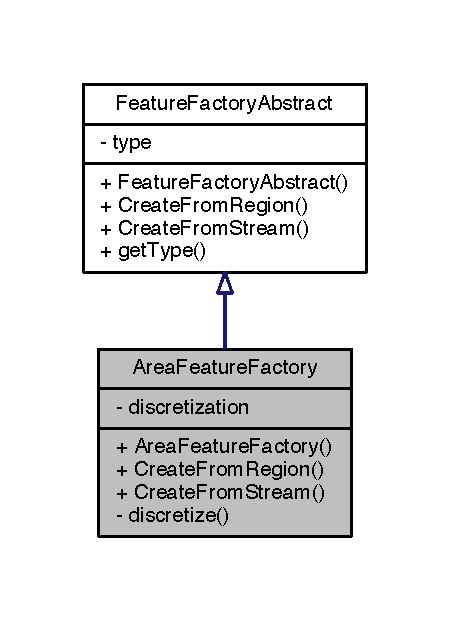
\includegraphics[width=222pt]{class_area_feature_factory__inherit__graph}
\end{center}
\end{figure}


Collaboration diagram for Area\+Feature\+Factory\+:\nopagebreak
\begin{figure}[H]
\begin{center}
\leavevmode
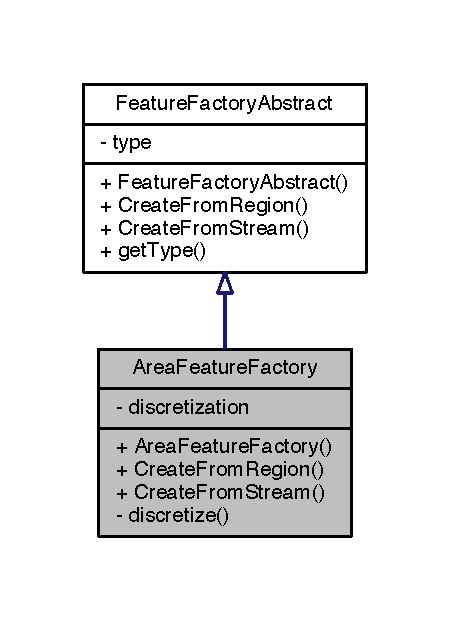
\includegraphics[width=222pt]{class_area_feature_factory__coll__graph}
\end{center}
\end{figure}


\subsection{Constructor \& Destructor Documentation}
\hypertarget{class_area_feature_factory_a1299cd28490bc46f5ee66e16b712e37d}{\index{Area\+Feature\+Factory@{Area\+Feature\+Factory}!Area\+Feature\+Factory@{Area\+Feature\+Factory}}
\index{Area\+Feature\+Factory@{Area\+Feature\+Factory}!Area\+Feature\+Factory@{Area\+Feature\+Factory}}
\subsubsection[{Area\+Feature\+Factory}]{\setlength{\rightskip}{0pt plus 5cm}Area\+Feature\+Factory\+::\+Area\+Feature\+Factory (
\begin{DoxyParamCaption}
\item[{int}]{discretization}
\end{DoxyParamCaption}
)}}\label{class_area_feature_factory_a1299cd28490bc46f5ee66e16b712e37d}


\subsection{Member Function Documentation}
\hypertarget{class_area_feature_factory_a241e29fcaf19c4756c7d01e86b272be3}{\index{Area\+Feature\+Factory@{Area\+Feature\+Factory}!Create\+From\+Region@{Create\+From\+Region}}
\index{Create\+From\+Region@{Create\+From\+Region}!Area\+Feature\+Factory@{Area\+Feature\+Factory}}
\subsubsection[{Create\+From\+Region}]{\setlength{\rightskip}{0pt plus 5cm}{\bf Feature\+Abstract\+Ptr} Area\+Feature\+Factory\+::\+Create\+From\+Region (
\begin{DoxyParamCaption}
\item[{const {\bf Region} $\ast$}]{region}
\end{DoxyParamCaption}
) const\hspace{0.3cm}{\ttfamily [virtual]}}}\label{class_area_feature_factory_a241e29fcaf19c4756c7d01e86b272be3}


Implements \hyperlink{class_feature_factory_abstract_a2b1aca909574b1828c8b019056656036}{Feature\+Factory\+Abstract}.



Here is the call graph for this function\+:\nopagebreak
\begin{figure}[H]
\begin{center}
\leavevmode
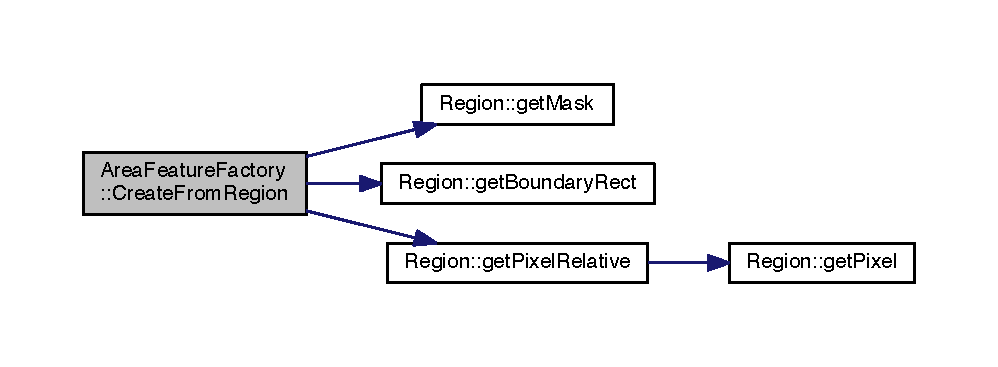
\includegraphics[width=350pt]{class_area_feature_factory_a241e29fcaf19c4756c7d01e86b272be3_cgraph}
\end{center}
\end{figure}


\hypertarget{class_area_feature_factory_ab8d7d3ebe9a928d340b4215d872e51ec}{\index{Area\+Feature\+Factory@{Area\+Feature\+Factory}!Create\+From\+Stream@{Create\+From\+Stream}}
\index{Create\+From\+Stream@{Create\+From\+Stream}!Area\+Feature\+Factory@{Area\+Feature\+Factory}}
\subsubsection[{Create\+From\+Stream}]{\setlength{\rightskip}{0pt plus 5cm}{\bf Feature\+Abstract\+Ptr} Area\+Feature\+Factory\+::\+Create\+From\+Stream (
\begin{DoxyParamCaption}
\item[{istream \&}]{stream}
\end{DoxyParamCaption}
) const\hspace{0.3cm}{\ttfamily [virtual]}}}\label{class_area_feature_factory_ab8d7d3ebe9a928d340b4215d872e51ec}


Implements \hyperlink{class_feature_factory_abstract_a32e7b404d34169840dae5ff1839da705}{Feature\+Factory\+Abstract}.

\hypertarget{class_area_feature_factory_a9e08ded8fb8dcf407edd0d7ec328129b}{\index{Area\+Feature\+Factory@{Area\+Feature\+Factory}!discretize@{discretize}}
\index{discretize@{discretize}!Area\+Feature\+Factory@{Area\+Feature\+Factory}}
\subsubsection[{discretize}]{\setlength{\rightskip}{0pt plus 5cm}void Area\+Feature\+Factory\+::discretize (
\begin{DoxyParamCaption}
\item[{int}]{quantization}
\end{DoxyParamCaption}
)\hspace{0.3cm}{\ttfamily [private]}}}\label{class_area_feature_factory_a9e08ded8fb8dcf407edd0d7ec328129b}


\subsection{Member Data Documentation}
\hypertarget{class_area_feature_factory_a77f36879829aeb6c25e7da509649b1ef}{\index{Area\+Feature\+Factory@{Area\+Feature\+Factory}!discretization@{discretization}}
\index{discretization@{discretization}!Area\+Feature\+Factory@{Area\+Feature\+Factory}}
\subsubsection[{discretization}]{\setlength{\rightskip}{0pt plus 5cm}int Area\+Feature\+Factory\+::discretization\hspace{0.3cm}{\ttfamily [private]}}}\label{class_area_feature_factory_a77f36879829aeb6c25e7da509649b1ef}


The documentation for this class was generated from the following files\+:\begin{DoxyCompactItemize}
\item 
Sources/\+Feature\+Extractors/\hyperlink{_area_feature_factory_8hpp}{Area\+Feature\+Factory.\+hpp}\item 
Sources/\+Feature\+Extractors/\hyperlink{_area_feature_factory_8cpp}{Area\+Feature\+Factory.\+cpp}\end{DoxyCompactItemize}

\hypertarget{classcompute__modularity_1_1_bt}{\section{compute\+\_\+modularity.\+Bt Class Reference}
\label{classcompute__modularity_1_1_bt}\index{compute\+\_\+modularity.\+Bt@{compute\+\_\+modularity.\+Bt}}
}
\subsection*{Static Private Attributes}
\begin{DoxyCompactItemize}
\item 
list \hyperlink{classcompute__modularity_1_1_bt_a67e24ec41d56d564d3c67e265cb9a4c3}{\+\_\+fields\+\_\+} = \mbox{[}('bt', c\+\_\+byte$\ast$16)\mbox{]}
\end{DoxyCompactItemize}


Inheritance diagram for compute\+\_\+modularity.\+Bt\+:\nopagebreak
\begin{figure}[H]
\begin{center}
\leavevmode
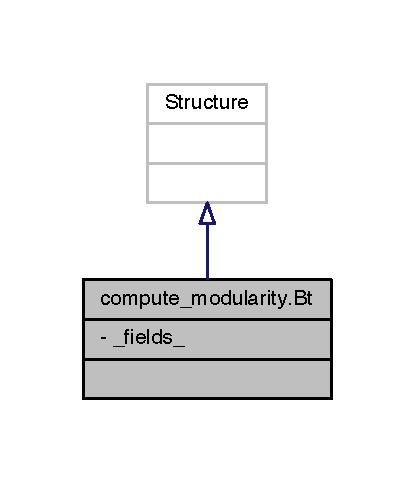
\includegraphics[width=199pt]{classcompute__modularity_1_1_bt__inherit__graph}
\end{center}
\end{figure}


Collaboration diagram for compute\+\_\+modularity.\+Bt\+:\nopagebreak
\begin{figure}[H]
\begin{center}
\leavevmode
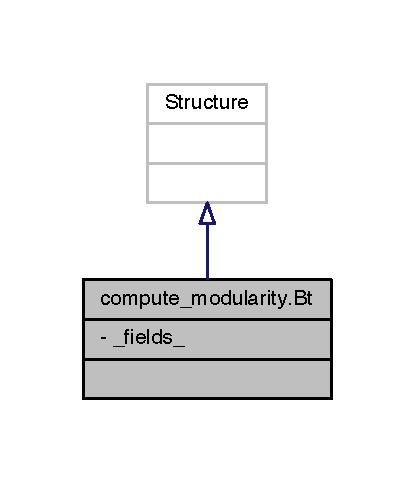
\includegraphics[width=199pt]{classcompute__modularity_1_1_bt__coll__graph}
\end{center}
\end{figure}


\subsection{Member Data Documentation}
\hypertarget{classcompute__modularity_1_1_bt_a67e24ec41d56d564d3c67e265cb9a4c3}{\index{compute\+\_\+modularity\+::\+Bt@{compute\+\_\+modularity\+::\+Bt}!\+\_\+fields\+\_\+@{\+\_\+fields\+\_\+}}
\index{\+\_\+fields\+\_\+@{\+\_\+fields\+\_\+}!compute\+\_\+modularity\+::\+Bt@{compute\+\_\+modularity\+::\+Bt}}
\subsubsection[{\+\_\+fields\+\_\+}]{\setlength{\rightskip}{0pt plus 5cm}list compute\+\_\+modularity.\+Bt.\+\_\+fields\+\_\+ = \mbox{[}('bt', c\+\_\+byte$\ast$16)\mbox{]}\hspace{0.3cm}{\ttfamily [static]}, {\ttfamily [private]}}}\label{classcompute__modularity_1_1_bt_a67e24ec41d56d564d3c67e265cb9a4c3}


The documentation for this class was generated from the following file\+:\begin{DoxyCompactItemize}
\item 
Sources/\+Experiments/\+Modularity\+\_\+py/\hyperlink{compute__modularity_8py}{compute\+\_\+modularity.\+py}\end{DoxyCompactItemize}

\hypertarget{class_cached_complex_network}{\section{Cached\+Complex\+Network$<$ N\+O\+D\+E\+\_\+\+T\+Y\+P\+E, E\+D\+G\+E\+\_\+\+T\+Y\+P\+E $>$ Class Template Reference}
\label{class_cached_complex_network}\index{Cached\+Complex\+Network$<$ N\+O\+D\+E\+\_\+\+T\+Y\+P\+E, E\+D\+G\+E\+\_\+\+T\+Y\+P\+E $>$@{Cached\+Complex\+Network$<$ N\+O\+D\+E\+\_\+\+T\+Y\+P\+E, E\+D\+G\+E\+\_\+\+T\+Y\+P\+E $>$}}
}


{\ttfamily \#include $<$Cached\+Complex\+Network.\+hpp$>$}

\subsection*{Public Member Functions}
\begin{DoxyCompactItemize}
\item 
\hyperlink{class_cached_complex_network_a47272a6c81ef87c488a7b3469af6a646}{Cached\+Complex\+Network} (bool \hyperlink{class_complex_network_ae1f8a32f89d84aab42475d8fe46dfa09}{directed}=true)
\item 
\hyperlink{_complex_network_8hpp_a8323334ca788fde39682469321590d52}{node\+\_\+id} \hyperlink{class_cached_complex_network_ad6e24699a050f5f2d7f908aba40b931c}{add\+Node} (const N\+O\+D\+E\+\_\+\+T\+Y\+P\+E \&n)
\item 
bool \hyperlink{class_cached_complex_network_a800aa02b94aa4bb73227e139cb246ddf}{remove\+Node} (\hyperlink{_complex_network_8hpp_a8323334ca788fde39682469321590d52}{node\+\_\+id} id)
\item 
\hyperlink{_complex_network_8hpp_a8323334ca788fde39682469321590d52}{node\+\_\+id} \hyperlink{class_cached_complex_network_ab3e77a01c6e77cc9983494174734f716}{get\+Node\+Id} (const N\+O\+D\+E\+\_\+\+T\+Y\+P\+E \&n)
\end{DoxyCompactItemize}
\subsection*{Private Attributes}
\begin{DoxyCompactItemize}
\item 
Q\+Hash$<$ N\+O\+D\+E\+\_\+\+T\+Y\+P\+E, \hyperlink{_complex_network_8hpp_a8323334ca788fde39682469321590d52}{node\+\_\+id} $>$ \hyperlink{class_cached_complex_network_ad0ac80eabd1a95fec5134a3fcbbe2f50}{cache}
\end{DoxyCompactItemize}
\subsection*{Additional Inherited Members}


Inheritance diagram for Cached\+Complex\+Network$<$ N\+O\+D\+E\+\_\+\+T\+Y\+P\+E, E\+D\+G\+E\+\_\+\+T\+Y\+P\+E $>$\+:\nopagebreak
\begin{figure}[H]
\begin{center}
\leavevmode
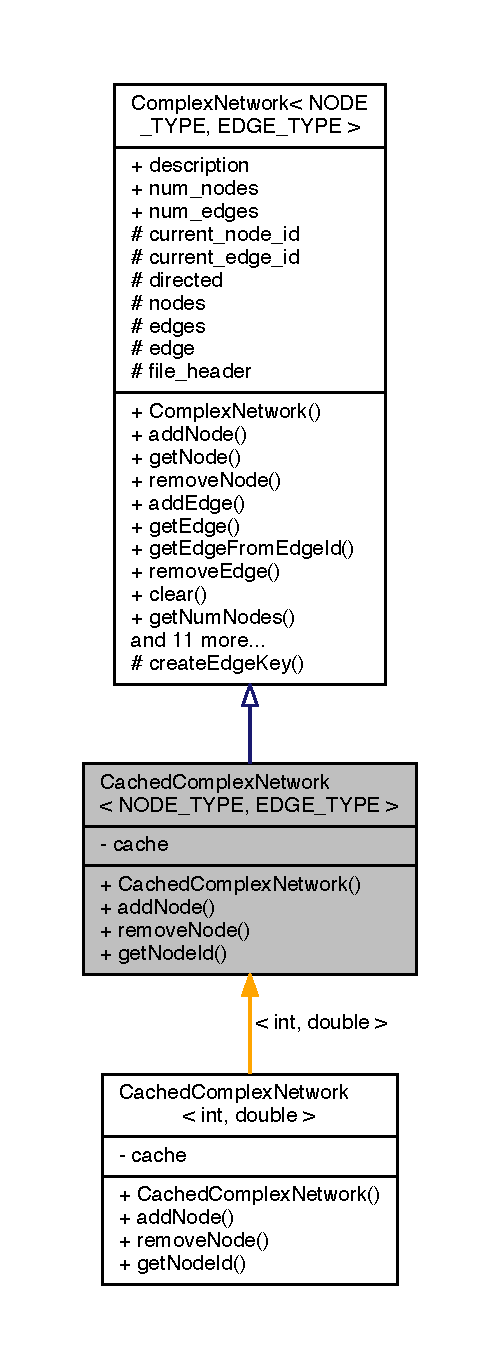
\includegraphics[height=550pt]{class_cached_complex_network__inherit__graph}
\end{center}
\end{figure}


Collaboration diagram for Cached\+Complex\+Network$<$ N\+O\+D\+E\+\_\+\+T\+Y\+P\+E, E\+D\+G\+E\+\_\+\+T\+Y\+P\+E $>$\+:\nopagebreak
\begin{figure}[H]
\begin{center}
\leavevmode
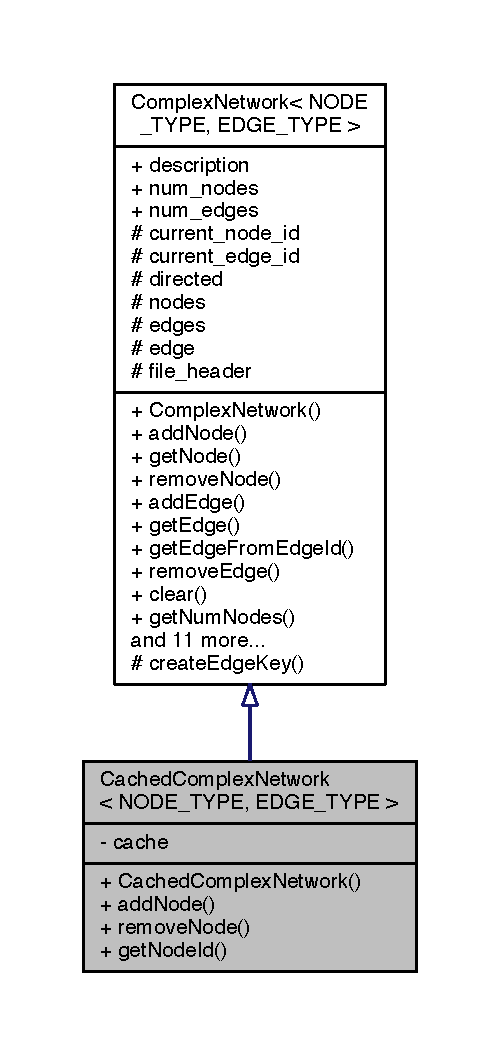
\includegraphics[width=240pt]{class_cached_complex_network__coll__graph}
\end{center}
\end{figure}


\subsection{Constructor \& Destructor Documentation}
\hypertarget{class_cached_complex_network_a47272a6c81ef87c488a7b3469af6a646}{\index{Cached\+Complex\+Network@{Cached\+Complex\+Network}!Cached\+Complex\+Network@{Cached\+Complex\+Network}}
\index{Cached\+Complex\+Network@{Cached\+Complex\+Network}!Cached\+Complex\+Network@{Cached\+Complex\+Network}}
\subsubsection[{Cached\+Complex\+Network}]{\setlength{\rightskip}{0pt plus 5cm}template$<$typename N\+O\+D\+E\+\_\+\+T\+Y\+P\+E , typename E\+D\+G\+E\+\_\+\+T\+Y\+P\+E $>$ {\bf Cached\+Complex\+Network}$<$ N\+O\+D\+E\+\_\+\+T\+Y\+P\+E, E\+D\+G\+E\+\_\+\+T\+Y\+P\+E $>$\+::{\bf Cached\+Complex\+Network} (
\begin{DoxyParamCaption}
\item[{bool}]{directed = {\ttfamily true}}
\end{DoxyParamCaption}
)}}\label{class_cached_complex_network_a47272a6c81ef87c488a7b3469af6a646}


\subsection{Member Function Documentation}
\hypertarget{class_cached_complex_network_ad6e24699a050f5f2d7f908aba40b931c}{\index{Cached\+Complex\+Network@{Cached\+Complex\+Network}!add\+Node@{add\+Node}}
\index{add\+Node@{add\+Node}!Cached\+Complex\+Network@{Cached\+Complex\+Network}}
\subsubsection[{add\+Node}]{\setlength{\rightskip}{0pt plus 5cm}template$<$typename N\+O\+D\+E\+\_\+\+T\+Y\+P\+E, typename E\+D\+G\+E\+\_\+\+T\+Y\+P\+E $>$ {\bf node\+\_\+id} {\bf Cached\+Complex\+Network}$<$ N\+O\+D\+E\+\_\+\+T\+Y\+P\+E, E\+D\+G\+E\+\_\+\+T\+Y\+P\+E $>$\+::add\+Node (
\begin{DoxyParamCaption}
\item[{const N\+O\+D\+E\+\_\+\+T\+Y\+P\+E \&}]{n}
\end{DoxyParamCaption}
)\hspace{0.3cm}{\ttfamily [virtual]}}}\label{class_cached_complex_network_ad6e24699a050f5f2d7f908aba40b931c}


Reimplemented from \hyperlink{class_complex_network_af2c31ca0d2142dafa1d88ca3ff22356f}{Complex\+Network$<$ N\+O\+D\+E\+\_\+\+T\+Y\+P\+E, E\+D\+G\+E\+\_\+\+T\+Y\+P\+E $>$}.



Here is the call graph for this function\+:\nopagebreak
\begin{figure}[H]
\begin{center}
\leavevmode
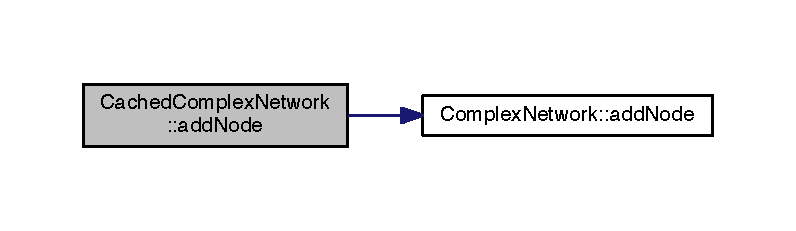
\includegraphics[width=350pt]{class_cached_complex_network_ad6e24699a050f5f2d7f908aba40b931c_cgraph}
\end{center}
\end{figure}




Here is the caller graph for this function\+:\nopagebreak
\begin{figure}[H]
\begin{center}
\leavevmode
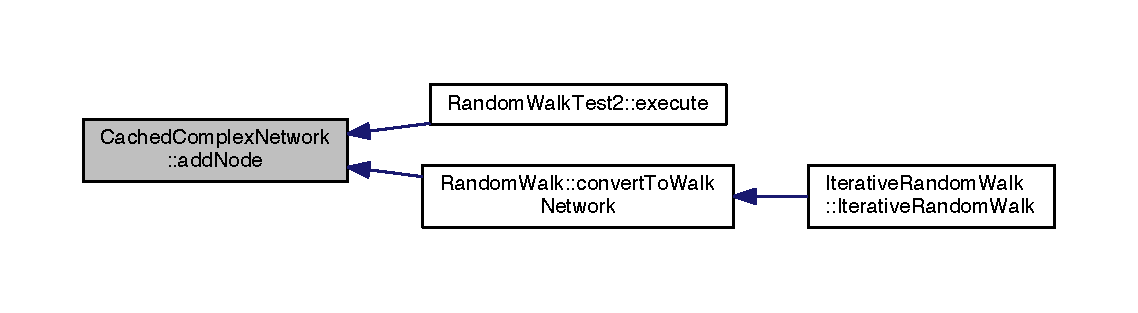
\includegraphics[width=350pt]{class_cached_complex_network_ad6e24699a050f5f2d7f908aba40b931c_icgraph}
\end{center}
\end{figure}


\hypertarget{class_cached_complex_network_ab3e77a01c6e77cc9983494174734f716}{\index{Cached\+Complex\+Network@{Cached\+Complex\+Network}!get\+Node\+Id@{get\+Node\+Id}}
\index{get\+Node\+Id@{get\+Node\+Id}!Cached\+Complex\+Network@{Cached\+Complex\+Network}}
\subsubsection[{get\+Node\+Id}]{\setlength{\rightskip}{0pt plus 5cm}template$<$typename N\+O\+D\+E\+\_\+\+T\+Y\+P\+E, typename E\+D\+G\+E\+\_\+\+T\+Y\+P\+E $>$ {\bf node\+\_\+id} {\bf Cached\+Complex\+Network}$<$ N\+O\+D\+E\+\_\+\+T\+Y\+P\+E, E\+D\+G\+E\+\_\+\+T\+Y\+P\+E $>$\+::get\+Node\+Id (
\begin{DoxyParamCaption}
\item[{const N\+O\+D\+E\+\_\+\+T\+Y\+P\+E \&}]{n}
\end{DoxyParamCaption}
)}}\label{class_cached_complex_network_ab3e77a01c6e77cc9983494174734f716}


Here is the caller graph for this function\+:\nopagebreak
\begin{figure}[H]
\begin{center}
\leavevmode
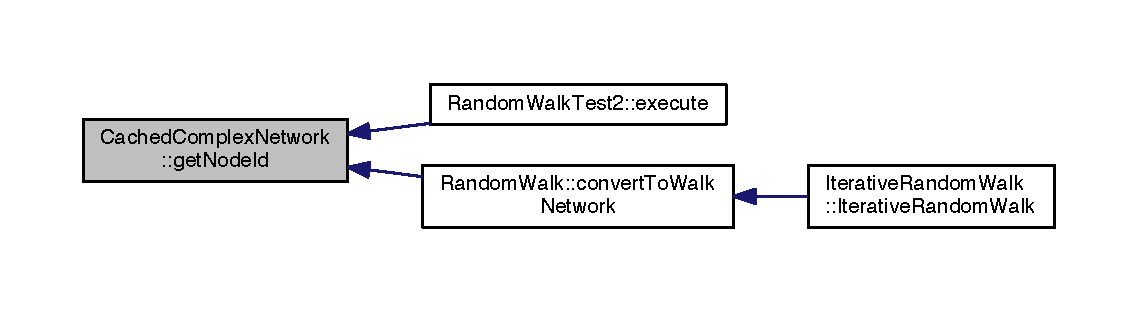
\includegraphics[width=350pt]{class_cached_complex_network_ab3e77a01c6e77cc9983494174734f716_icgraph}
\end{center}
\end{figure}


\hypertarget{class_cached_complex_network_a800aa02b94aa4bb73227e139cb246ddf}{\index{Cached\+Complex\+Network@{Cached\+Complex\+Network}!remove\+Node@{remove\+Node}}
\index{remove\+Node@{remove\+Node}!Cached\+Complex\+Network@{Cached\+Complex\+Network}}
\subsubsection[{remove\+Node}]{\setlength{\rightskip}{0pt plus 5cm}template$<$typename N\+O\+D\+E\+\_\+\+T\+Y\+P\+E , typename E\+D\+G\+E\+\_\+\+T\+Y\+P\+E $>$ bool {\bf Cached\+Complex\+Network}$<$ N\+O\+D\+E\+\_\+\+T\+Y\+P\+E, E\+D\+G\+E\+\_\+\+T\+Y\+P\+E $>$\+::remove\+Node (
\begin{DoxyParamCaption}
\item[{{\bf node\+\_\+id}}]{id}
\end{DoxyParamCaption}
)\hspace{0.3cm}{\ttfamily [virtual]}}}\label{class_cached_complex_network_a800aa02b94aa4bb73227e139cb246ddf}


Reimplemented from \hyperlink{class_complex_network_a33f2b4528cc31296ede98be7e6dcd600}{Complex\+Network$<$ N\+O\+D\+E\+\_\+\+T\+Y\+P\+E, E\+D\+G\+E\+\_\+\+T\+Y\+P\+E $>$}.



Here is the call graph for this function\+:\nopagebreak
\begin{figure}[H]
\begin{center}
\leavevmode
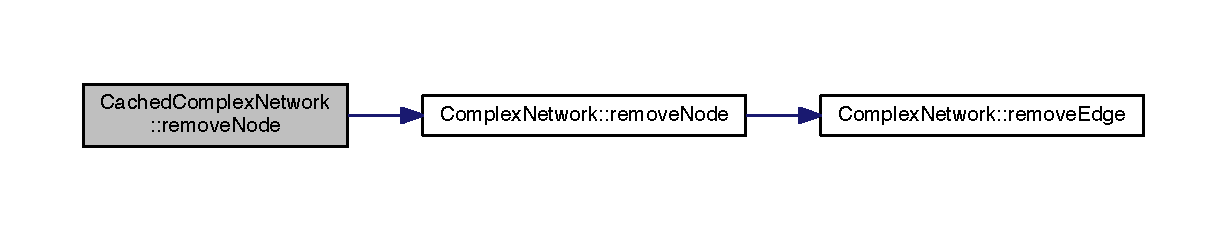
\includegraphics[width=350pt]{class_cached_complex_network_a800aa02b94aa4bb73227e139cb246ddf_cgraph}
\end{center}
\end{figure}




\subsection{Member Data Documentation}
\hypertarget{class_cached_complex_network_ad0ac80eabd1a95fec5134a3fcbbe2f50}{\index{Cached\+Complex\+Network@{Cached\+Complex\+Network}!cache@{cache}}
\index{cache@{cache}!Cached\+Complex\+Network@{Cached\+Complex\+Network}}
\subsubsection[{cache}]{\setlength{\rightskip}{0pt plus 5cm}template$<$typename N\+O\+D\+E\+\_\+\+T\+Y\+P\+E, typename E\+D\+G\+E\+\_\+\+T\+Y\+P\+E$>$ Q\+Hash$<$N\+O\+D\+E\+\_\+\+T\+Y\+P\+E, {\bf node\+\_\+id}$>$ {\bf Cached\+Complex\+Network}$<$ N\+O\+D\+E\+\_\+\+T\+Y\+P\+E, E\+D\+G\+E\+\_\+\+T\+Y\+P\+E $>$\+::cache\hspace{0.3cm}{\ttfamily [private]}}}\label{class_cached_complex_network_ad0ac80eabd1a95fec5134a3fcbbe2f50}


The documentation for this class was generated from the following file\+:\begin{DoxyCompactItemize}
\item 
Sources/\+Utilities/\hyperlink{_cached_complex_network_8hpp}{Cached\+Complex\+Network.\+hpp}\end{DoxyCompactItemize}

\hypertarget{class_complex_network}{\section{Complex\+Network$<$ N\+O\+D\+E\+\_\+\+T\+Y\+P\+E, E\+D\+G\+E\+\_\+\+T\+Y\+P\+E $>$ Class Template Reference}
\label{class_complex_network}\index{Complex\+Network$<$ N\+O\+D\+E\+\_\+\+T\+Y\+P\+E, E\+D\+G\+E\+\_\+\+T\+Y\+P\+E $>$@{Complex\+Network$<$ N\+O\+D\+E\+\_\+\+T\+Y\+P\+E, E\+D\+G\+E\+\_\+\+T\+Y\+P\+E $>$}}
}


{\ttfamily \#include $<$Complex\+Network.\+hpp$>$}

\subsection*{Classes}
\begin{DoxyCompactItemize}
\item 
class \hyperlink{class_complex_network_1_1_edge_iterator}{Edge\+Iterator}
\item 
class \hyperlink{class_complex_network_1_1_node_iterator}{Node\+Iterator}
\end{DoxyCompactItemize}
\subsection*{Public Member Functions}
\begin{DoxyCompactItemize}
\item 
\hyperlink{class_complex_network_a4a16e825e1d8b487067ca21d677617a3}{Complex\+Network} (bool \hyperlink{class_complex_network_ae1f8a32f89d84aab42475d8fe46dfa09}{directed}=true)
\item 
virtual \hyperlink{_complex_network_8hpp_a8323334ca788fde39682469321590d52}{node\+\_\+id} \hyperlink{class_complex_network_af2c31ca0d2142dafa1d88ca3ff22356f}{add\+Node} (const N\+O\+D\+E\+\_\+\+T\+Y\+P\+E \&n)
\item 
virtual N\+O\+D\+E\+\_\+\+T\+Y\+P\+E $\ast$ \hyperlink{class_complex_network_a3711aff250a942a9ad61d0571be82c43}{get\+Node} (\hyperlink{_complex_network_8hpp_a8323334ca788fde39682469321590d52}{node\+\_\+id} id)
\item 
virtual bool \hyperlink{class_complex_network_a33f2b4528cc31296ede98be7e6dcd600}{remove\+Node} (\hyperlink{_complex_network_8hpp_a8323334ca788fde39682469321590d52}{node\+\_\+id} id)
\item 
virtual void \hyperlink{class_complex_network_a52c25eb9c9c642a39681e4040fc0a17d}{add\+Edge} (\hyperlink{_complex_network_8hpp_a8323334ca788fde39682469321590d52}{node\+\_\+id} from, \hyperlink{_complex_network_8hpp_a8323334ca788fde39682469321590d52}{node\+\_\+id} to, const E\+D\+G\+E\+\_\+\+T\+Y\+P\+E \&e)
\item 
virtual E\+D\+G\+E\+\_\+\+T\+Y\+P\+E $\ast$ \hyperlink{class_complex_network_a6a1c638e4604efe06c12ce3065020ec1}{get\+Edge} (\hyperlink{_complex_network_8hpp_a8323334ca788fde39682469321590d52}{node\+\_\+id} from, \hyperlink{_complex_network_8hpp_a8323334ca788fde39682469321590d52}{node\+\_\+id} to)
\item 
virtual E\+D\+G\+E\+\_\+\+T\+Y\+P\+E $\ast$ \hyperlink{class_complex_network_ad440008416fc33500754d77b2532560f}{get\+Edge\+From\+Edge\+Id} (\hyperlink{_complex_network_8hpp_ad7d18d7b90a45b6625704e92d10aa3a0}{edge\+\_\+id} id)
\item 
virtual bool \hyperlink{class_complex_network_a9b2c7df561a2ad5fc14b04a5c5c56828}{remove\+Edge} (\hyperlink{_complex_network_8hpp_a8323334ca788fde39682469321590d52}{node\+\_\+id} from, \hyperlink{_complex_network_8hpp_a8323334ca788fde39682469321590d52}{node\+\_\+id} to)
\item 
virtual void \hyperlink{class_complex_network_a64db5949375a84eba3d9ff559d68fc6e}{clear} ()
\item 
unsigned int \hyperlink{class_complex_network_afee98f26ceed674c17be01a740787170}{get\+Num\+Nodes} () const 
\item 
unsigned int \hyperlink{class_complex_network_a720cb4e40342648d394792cc693d29a5}{get\+Num\+Edges} () const 
\item 
\hyperlink{class_complex_network_1_1_node_iterator}{Node\+Iterator} \hyperlink{class_complex_network_ab02bc6912437322f146f6ce98b415759}{Begin} ()
\item 
\hyperlink{class_complex_network_1_1_node_iterator}{Node\+Iterator} \hyperlink{class_complex_network_a2c90f4efd046776d7a53776b24daae0f}{End} ()
\item 
\hyperlink{class_complex_network_1_1_edge_iterator}{Edge\+Iterator} \hyperlink{class_complex_network_a2167b224079f5c0b44443959ad0b6440}{Edges\+Begin} (\hyperlink{_complex_network_8hpp_a8323334ca788fde39682469321590d52}{node\+\_\+id} node\+\_\+from)
\item 
\hyperlink{class_complex_network_1_1_edge_iterator}{Edge\+Iterator} \hyperlink{class_complex_network_ad806138ea94ec18ed17f4681ab731208}{Edges\+End} (\hyperlink{_complex_network_8hpp_a8323334ca788fde39682469321590d52}{node\+\_\+id} node\+\_\+from)
\item 
\hyperlink{class_complex_network_1_1_edge_iterator}{Edge\+Iterator} \hyperlink{class_complex_network_a3a228b9a9497db2b9385deb4eb39f1e1}{Edges\+Begin} ()
\item 
\hyperlink{class_complex_network_1_1_edge_iterator}{Edge\+Iterator} \hyperlink{class_complex_network_afa7d628b66a815d97afbf5373640d12b}{Edges\+End} ()
\item 
unsigned int \hyperlink{class_complex_network_a4036d2cda2dc5596d03e164c3455aff6}{get\+Num\+Edges} (\hyperlink{_complex_network_8hpp_a8323334ca788fde39682469321590d52}{node\+\_\+id}) const 
\item 
void \hyperlink{class_complex_network_a5d127d4296808b7ccdadccaa58084e96}{save} (const char $\ast$filename)
\item 
void \hyperlink{class_complex_network_a54fbdb35418f424e8dad0dbc5dc16bee}{load} (const char $\ast$filename)
\item 
\hyperlink{class_complex_network}{Complex\+Network}$<$ N\+O\+D\+E\+\_\+\+T\+Y\+P\+E, \\*
E\+D\+G\+E\+\_\+\+T\+Y\+P\+E $>$ \& \hyperlink{class_complex_network_a5a8b07f5ca5d247e13a2e2bc5ac75de1}{operator=} (const \hyperlink{class_complex_network}{Complex\+Network}$<$ N\+O\+D\+E\+\_\+\+T\+Y\+P\+E, E\+D\+G\+E\+\_\+\+T\+Y\+P\+E $>$ \&cn)
\end{DoxyCompactItemize}
\subsection*{Protected Member Functions}
\begin{DoxyCompactItemize}
\item 
Q\+Pair$<$ \hyperlink{_complex_network_8hpp_a8323334ca788fde39682469321590d52}{node\+\_\+id}, \hyperlink{_complex_network_8hpp_a8323334ca788fde39682469321590d52}{node\+\_\+id} $>$ \hyperlink{class_complex_network_a982b0db93143ff949025e326794af02d}{create\+Edge\+Key} (\hyperlink{_complex_network_8hpp_a8323334ca788fde39682469321590d52}{node\+\_\+id} from, \hyperlink{_complex_network_8hpp_a8323334ca788fde39682469321590d52}{node\+\_\+id} to)
\end{DoxyCompactItemize}
\subsection*{Protected Attributes}
\begin{DoxyCompactItemize}
\item 
\hyperlink{_complex_network_8hpp_a8323334ca788fde39682469321590d52}{node\+\_\+id} \hyperlink{class_complex_network_ab71dc127e36a989049df28f58f2c315a}{current\+\_\+node\+\_\+id}
\item 
\hyperlink{_complex_network_8hpp_ad7d18d7b90a45b6625704e92d10aa3a0}{edge\+\_\+id} \hyperlink{class_complex_network_a5305dba65a6d949064e46a6729c39e53}{current\+\_\+edge\+\_\+id}
\item 
bool \hyperlink{class_complex_network_ae1f8a32f89d84aab42475d8fe46dfa09}{directed}
\item 
Q\+Hash$<$ \hyperlink{_complex_network_8hpp_a8323334ca788fde39682469321590d52}{node\+\_\+id}, N\+O\+D\+E\+\_\+\+T\+Y\+P\+E $>$ \hyperlink{class_complex_network_a6b0ecc57af689b9ba9f8855132d1c275}{nodes}
\item 
Q\+Hash$<$ \hyperlink{_complex_network_8hpp_a8323334ca788fde39682469321590d52}{node\+\_\+id}, Q\+Hash$<$ \hyperlink{_complex_network_8hpp_a8323334ca788fde39682469321590d52}{node\+\_\+id}, \\*
\hyperlink{_complex_network_8hpp_ad7d18d7b90a45b6625704e92d10aa3a0}{edge\+\_\+id} $>$ $>$ \hyperlink{class_complex_network_adbdf613ffde926399cd5f6e7b8c09536}{edges}
\item 
Q\+Hash$<$ \hyperlink{_complex_network_8hpp_ad7d18d7b90a45b6625704e92d10aa3a0}{edge\+\_\+id}, E\+D\+G\+E\+\_\+\+T\+Y\+P\+E $>$ \hyperlink{class_complex_network_a666bb7ad7f5ab90416f037aeb1ba11d0}{edge}
\item 
\begin{tabbing}
xx\=xx\=xx\=xx\=xx\=xx\=xx\=xx\=xx\=\kill
struct \{\\
\>char \hyperlink{class_complex_network_abc2c2def62701d56ec56c8b0accbedb9}{description} \mbox{[}200\mbox{]}\\
\>unsigned int \hyperlink{class_complex_network_a6c8777ba48e68c02d2d523abe904b6b1}{num\_nodes}\\
\>unsigned int \hyperlink{class_complex_network_ac4a7f179af0187eb3071969642b445cc}{num\_edges}\\
\} \hyperlink{class_complex_network_ab9ab3dbbbcd8dd173ec40938391c0fc4}{file\_header}\\

\end{tabbing}\end{DoxyCompactItemize}


Inheritance diagram for Complex\+Network$<$ N\+O\+D\+E\+\_\+\+T\+Y\+P\+E, E\+D\+G\+E\+\_\+\+T\+Y\+P\+E $>$\+:\nopagebreak
\begin{figure}[H]
\begin{center}
\leavevmode
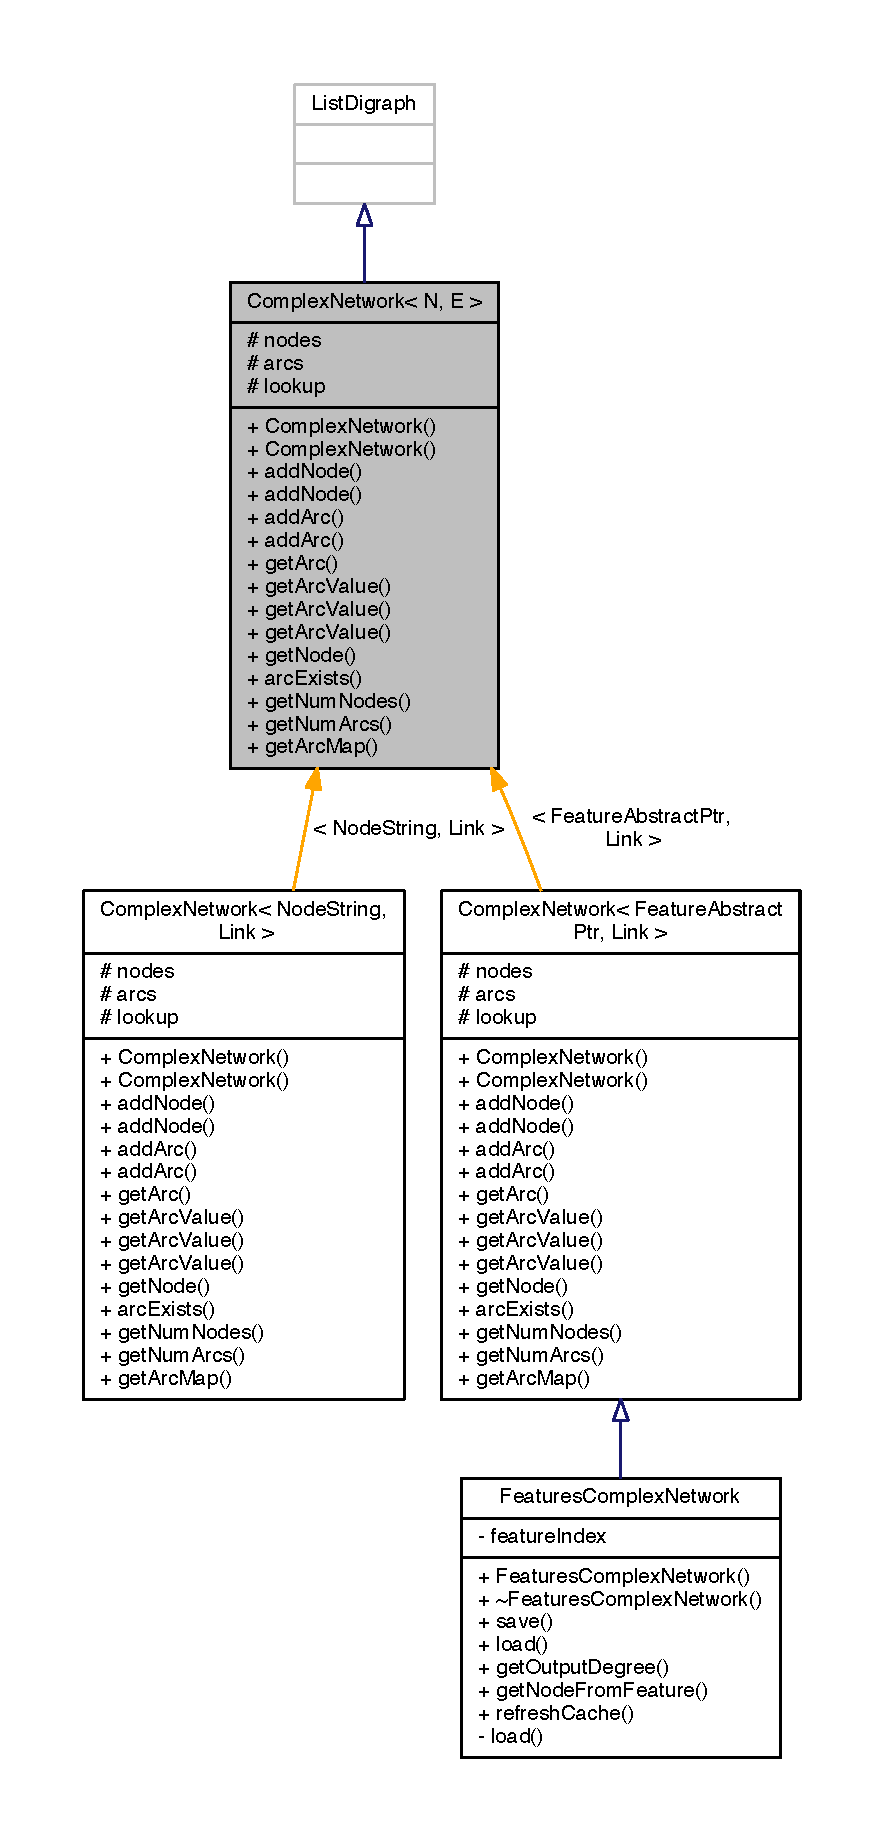
\includegraphics[width=254pt]{class_complex_network__inherit__graph}
\end{center}
\end{figure}


Collaboration diagram for Complex\+Network$<$ N\+O\+D\+E\+\_\+\+T\+Y\+P\+E, E\+D\+G\+E\+\_\+\+T\+Y\+P\+E $>$\+:\nopagebreak
\begin{figure}[H]
\begin{center}
\leavevmode
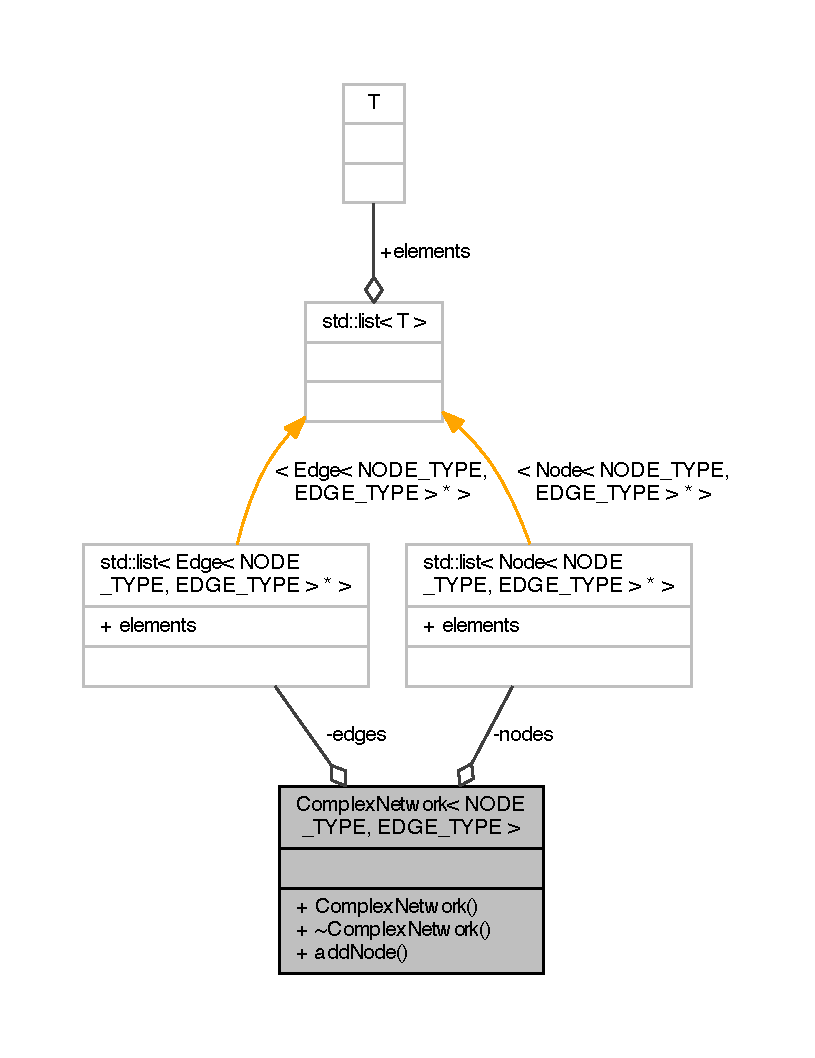
\includegraphics[width=350pt]{class_complex_network__coll__graph}
\end{center}
\end{figure}


\subsection{Constructor \& Destructor Documentation}
\hypertarget{class_complex_network_a4a16e825e1d8b487067ca21d677617a3}{\index{Complex\+Network@{Complex\+Network}!Complex\+Network@{Complex\+Network}}
\index{Complex\+Network@{Complex\+Network}!Complex\+Network@{Complex\+Network}}
\subsubsection[{Complex\+Network}]{\setlength{\rightskip}{0pt plus 5cm}template$<$typename N\+O\+D\+E\+\_\+\+T\+Y\+P\+E , typename E\+D\+G\+E\+\_\+\+T\+Y\+P\+E $>$ {\bf Complex\+Network}$<$ N\+O\+D\+E\+\_\+\+T\+Y\+P\+E, E\+D\+G\+E\+\_\+\+T\+Y\+P\+E $>$\+::{\bf Complex\+Network} (
\begin{DoxyParamCaption}
\item[{bool}]{directed = {\ttfamily true}}
\end{DoxyParamCaption}
)}}\label{class_complex_network_a4a16e825e1d8b487067ca21d677617a3}


\subsection{Member Function Documentation}
\hypertarget{class_complex_network_a52c25eb9c9c642a39681e4040fc0a17d}{\index{Complex\+Network@{Complex\+Network}!add\+Edge@{add\+Edge}}
\index{add\+Edge@{add\+Edge}!Complex\+Network@{Complex\+Network}}
\subsubsection[{add\+Edge}]{\setlength{\rightskip}{0pt plus 5cm}template$<$typename N\+O\+D\+E\+\_\+\+T\+Y\+P\+E , typename E\+D\+G\+E\+\_\+\+T\+Y\+P\+E$>$ void {\bf Complex\+Network}$<$ N\+O\+D\+E\+\_\+\+T\+Y\+P\+E, E\+D\+G\+E\+\_\+\+T\+Y\+P\+E $>$\+::add\+Edge (
\begin{DoxyParamCaption}
\item[{{\bf node\+\_\+id}}]{from, }
\item[{{\bf node\+\_\+id}}]{to, }
\item[{const E\+D\+G\+E\+\_\+\+T\+Y\+P\+E \&}]{e}
\end{DoxyParamCaption}
)\hspace{0.3cm}{\ttfamily [virtual]}}}\label{class_complex_network_a52c25eb9c9c642a39681e4040fc0a17d}


Here is the caller graph for this function\+:
\nopagebreak
\begin{figure}[H]
\begin{center}
\leavevmode
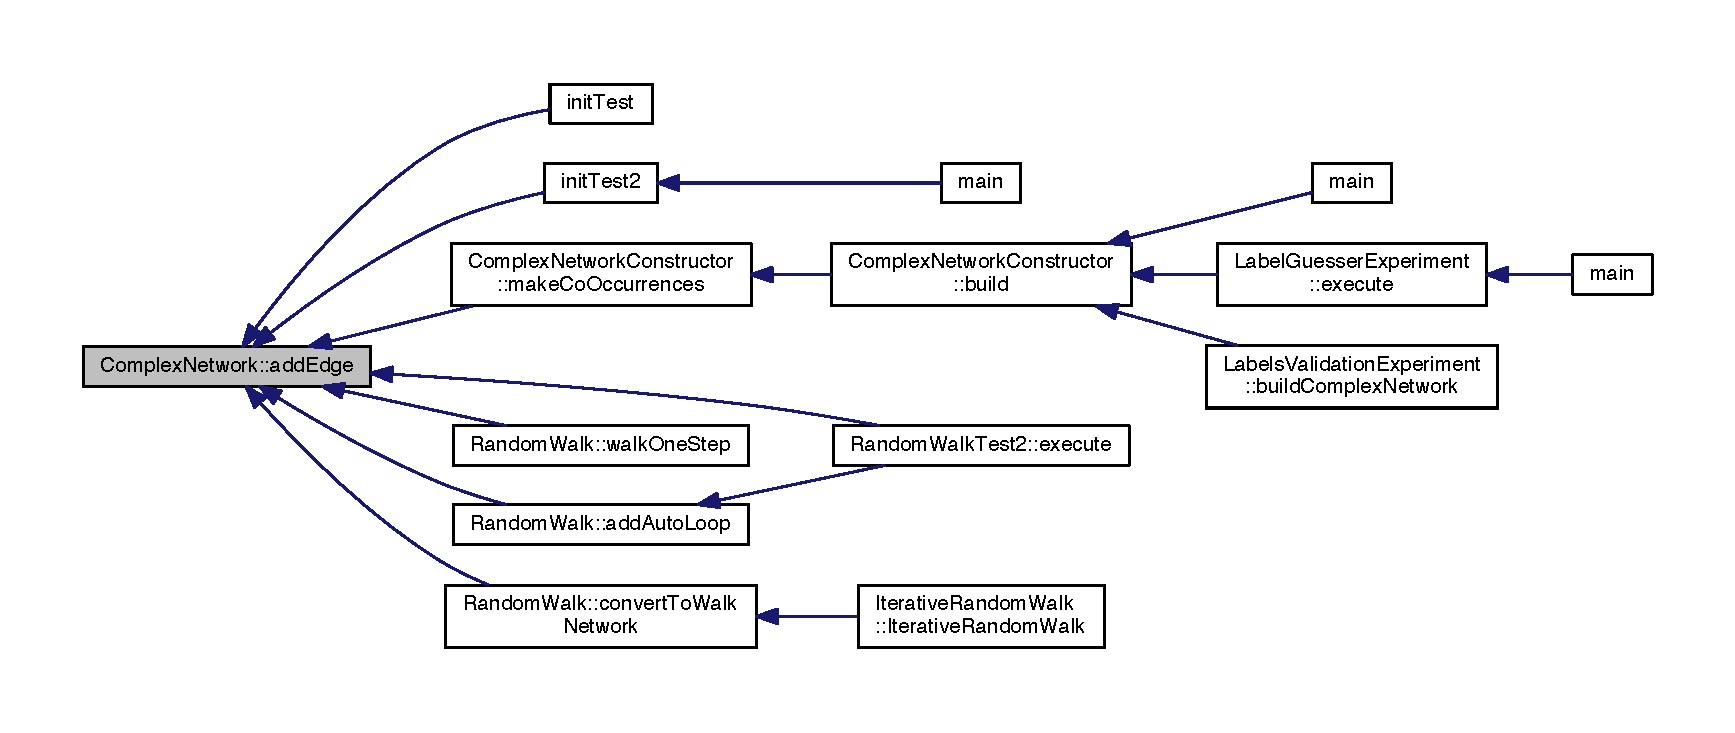
\includegraphics[width=350pt]{class_complex_network_a52c25eb9c9c642a39681e4040fc0a17d_icgraph}
\end{center}
\end{figure}


\hypertarget{class_complex_network_af2c31ca0d2142dafa1d88ca3ff22356f}{\index{Complex\+Network@{Complex\+Network}!add\+Node@{add\+Node}}
\index{add\+Node@{add\+Node}!Complex\+Network@{Complex\+Network}}
\subsubsection[{add\+Node}]{\setlength{\rightskip}{0pt plus 5cm}template$<$typename N\+O\+D\+E\+\_\+\+T\+Y\+P\+E, typename E\+D\+G\+E\+\_\+\+T\+Y\+P\+E $>$ {\bf node\+\_\+id} {\bf Complex\+Network}$<$ N\+O\+D\+E\+\_\+\+T\+Y\+P\+E, E\+D\+G\+E\+\_\+\+T\+Y\+P\+E $>$\+::add\+Node (
\begin{DoxyParamCaption}
\item[{const N\+O\+D\+E\+\_\+\+T\+Y\+P\+E \&}]{n}
\end{DoxyParamCaption}
)\hspace{0.3cm}{\ttfamily [virtual]}}}\label{class_complex_network_af2c31ca0d2142dafa1d88ca3ff22356f}


Reimplemented in \hyperlink{class_cached_complex_network_ad6e24699a050f5f2d7f908aba40b931c}{Cached\+Complex\+Network$<$ N\+O\+D\+E\+\_\+\+T\+Y\+P\+E, E\+D\+G\+E\+\_\+\+T\+Y\+P\+E $>$}, and \hyperlink{class_cached_complex_network_ad6e24699a050f5f2d7f908aba40b931c}{Cached\+Complex\+Network$<$ int, double $>$}.



Here is the caller graph for this function\+:
\nopagebreak
\begin{figure}[H]
\begin{center}
\leavevmode
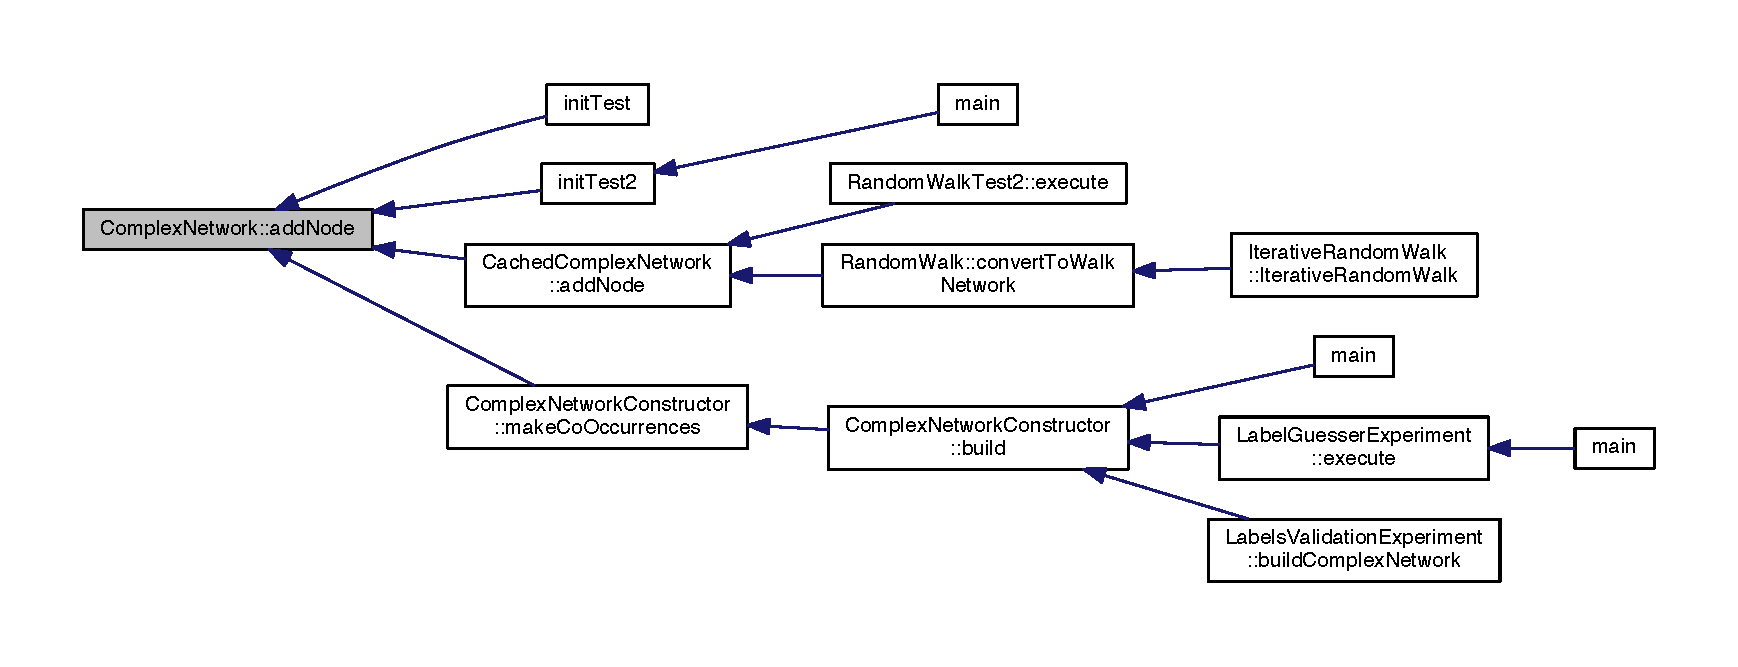
\includegraphics[width=350pt]{class_complex_network_af2c31ca0d2142dafa1d88ca3ff22356f_icgraph}
\end{center}
\end{figure}


\hypertarget{class_complex_network_ab02bc6912437322f146f6ce98b415759}{\index{Complex\+Network@{Complex\+Network}!Begin@{Begin}}
\index{Begin@{Begin}!Complex\+Network@{Complex\+Network}}
\subsubsection[{Begin}]{\setlength{\rightskip}{0pt plus 5cm}template$<$typename N\+O\+D\+E\+\_\+\+T\+Y\+P\+E , typename E\+D\+G\+E\+\_\+\+T\+Y\+P\+E $>$ {\bf Complex\+Network}$<$ N\+O\+D\+E\+\_\+\+T\+Y\+P\+E, E\+D\+G\+E\+\_\+\+T\+Y\+P\+E $>$\+::{\bf Node\+Iterator} {\bf Complex\+Network}$<$ N\+O\+D\+E\+\_\+\+T\+Y\+P\+E, E\+D\+G\+E\+\_\+\+T\+Y\+P\+E $>$\+::Begin (
\begin{DoxyParamCaption}
{}
\end{DoxyParamCaption}
)}}\label{class_complex_network_ab02bc6912437322f146f6ce98b415759}


Here is the caller graph for this function\+:
\nopagebreak
\begin{figure}[H]
\begin{center}
\leavevmode
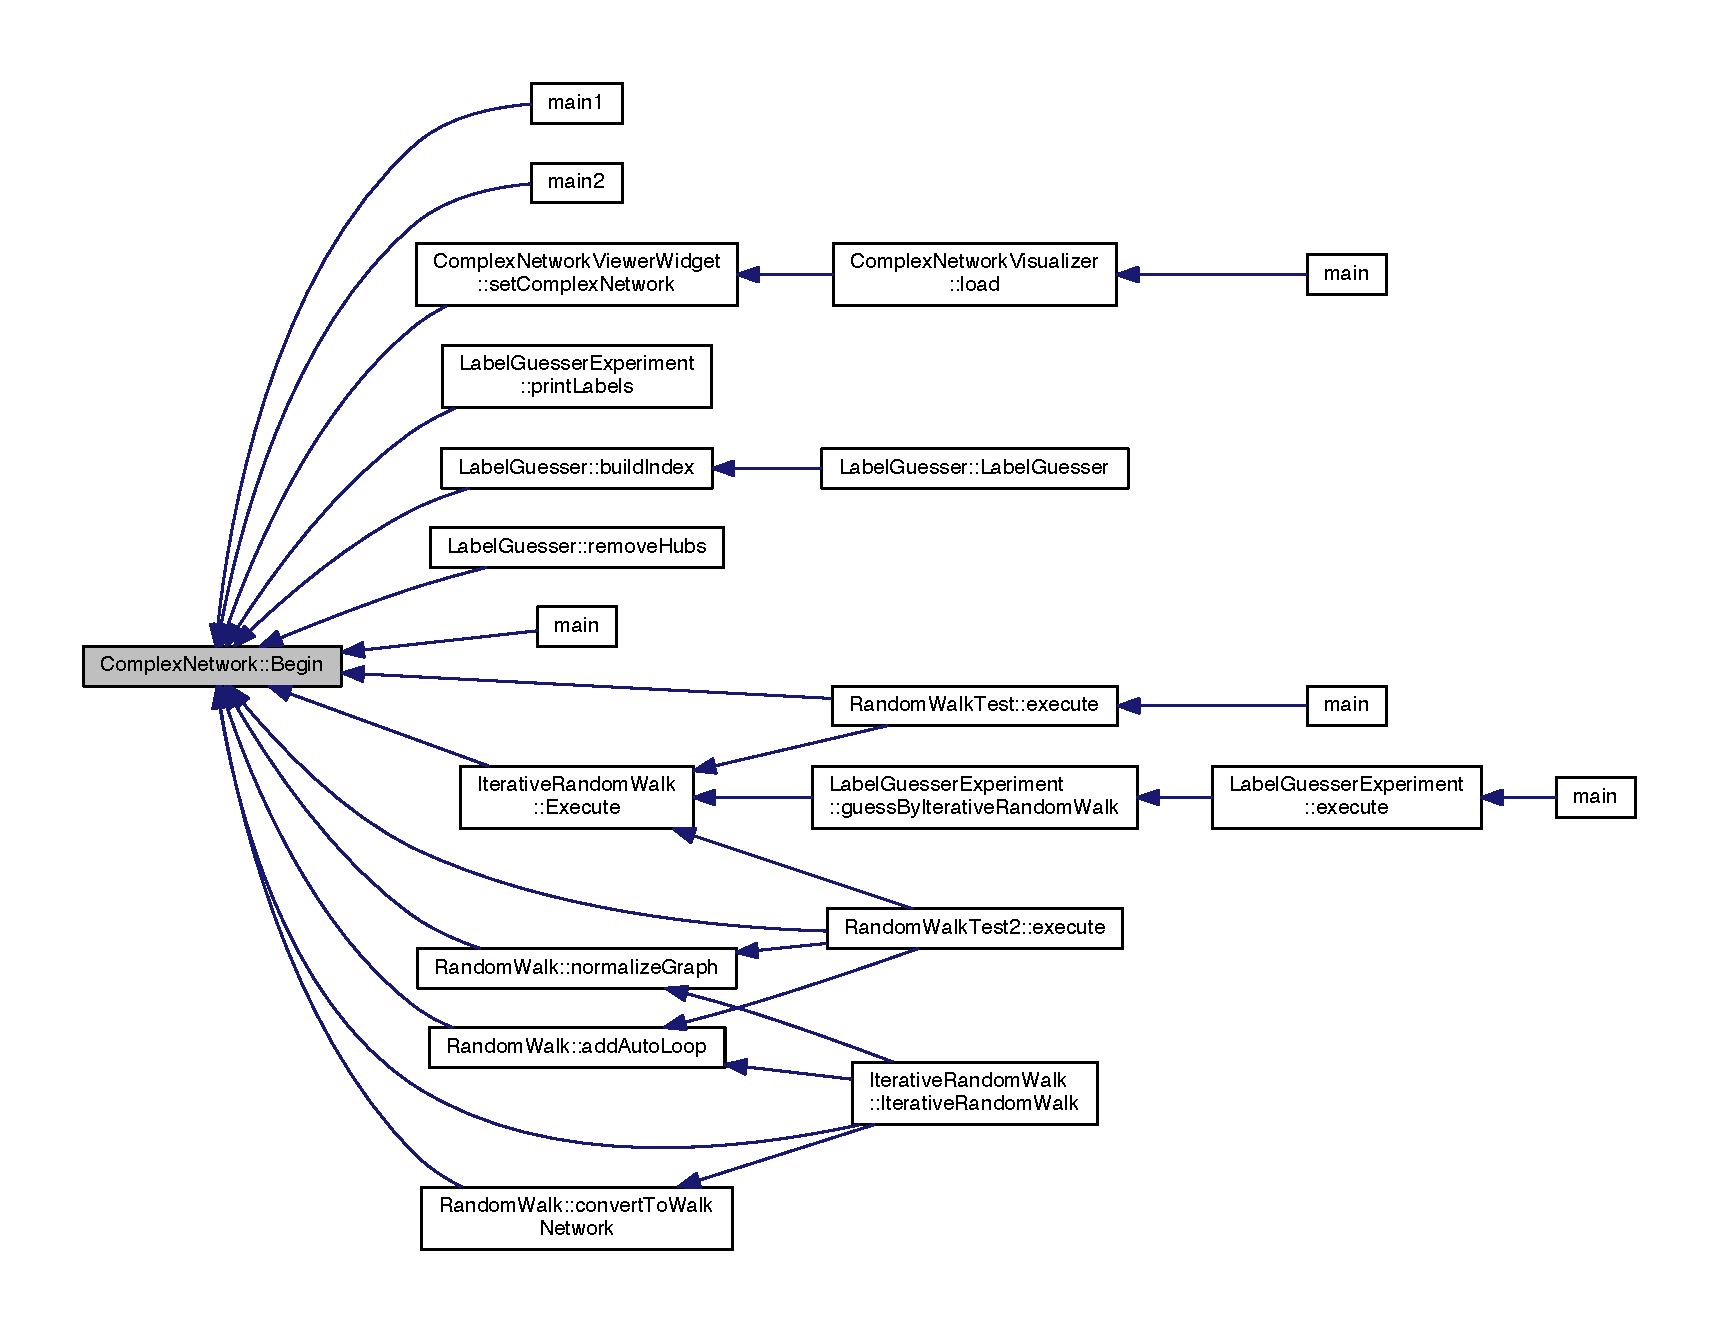
\includegraphics[width=350pt]{class_complex_network_ab02bc6912437322f146f6ce98b415759_icgraph}
\end{center}
\end{figure}


\hypertarget{class_complex_network_a64db5949375a84eba3d9ff559d68fc6e}{\index{Complex\+Network@{Complex\+Network}!clear@{clear}}
\index{clear@{clear}!Complex\+Network@{Complex\+Network}}
\subsubsection[{clear}]{\setlength{\rightskip}{0pt plus 5cm}template$<$typename N\+O\+D\+E\+\_\+\+T\+Y\+P\+E , typename E\+D\+G\+E\+\_\+\+T\+Y\+P\+E $>$ void {\bf Complex\+Network}$<$ N\+O\+D\+E\+\_\+\+T\+Y\+P\+E, E\+D\+G\+E\+\_\+\+T\+Y\+P\+E $>$\+::clear (
\begin{DoxyParamCaption}
{}
\end{DoxyParamCaption}
)\hspace{0.3cm}{\ttfamily [virtual]}}}\label{class_complex_network_a64db5949375a84eba3d9ff559d68fc6e}


Reimplemented in \hyperlink{class_features_complex_network_a747eba83de2a19a39e3d9f230d055d59}{Features\+Complex\+Network}.

\hypertarget{class_complex_network_a982b0db93143ff949025e326794af02d}{\index{Complex\+Network@{Complex\+Network}!create\+Edge\+Key@{create\+Edge\+Key}}
\index{create\+Edge\+Key@{create\+Edge\+Key}!Complex\+Network@{Complex\+Network}}
\subsubsection[{create\+Edge\+Key}]{\setlength{\rightskip}{0pt plus 5cm}template$<$typename N\+O\+D\+E\+\_\+\+T\+Y\+P\+E , typename E\+D\+G\+E\+\_\+\+T\+Y\+P\+E $>$ Q\+Pair$<$ {\bf node\+\_\+id}, {\bf node\+\_\+id} $>$ {\bf Complex\+Network}$<$ N\+O\+D\+E\+\_\+\+T\+Y\+P\+E, E\+D\+G\+E\+\_\+\+T\+Y\+P\+E $>$\+::create\+Edge\+Key (
\begin{DoxyParamCaption}
\item[{{\bf node\+\_\+id}}]{from, }
\item[{{\bf node\+\_\+id}}]{to}
\end{DoxyParamCaption}
)\hspace{0.3cm}{\ttfamily [inline]}, {\ttfamily [protected]}}}\label{class_complex_network_a982b0db93143ff949025e326794af02d}
\hypertarget{class_complex_network_a2167b224079f5c0b44443959ad0b6440}{\index{Complex\+Network@{Complex\+Network}!Edges\+Begin@{Edges\+Begin}}
\index{Edges\+Begin@{Edges\+Begin}!Complex\+Network@{Complex\+Network}}
\subsubsection[{Edges\+Begin}]{\setlength{\rightskip}{0pt plus 5cm}template$<$typename N\+O\+D\+E\+\_\+\+T\+Y\+P\+E , typename E\+D\+G\+E\+\_\+\+T\+Y\+P\+E $>$ {\bf Complex\+Network}$<$ N\+O\+D\+E\+\_\+\+T\+Y\+P\+E, E\+D\+G\+E\+\_\+\+T\+Y\+P\+E $>$\+::{\bf Edge\+Iterator} {\bf Complex\+Network}$<$ N\+O\+D\+E\+\_\+\+T\+Y\+P\+E, E\+D\+G\+E\+\_\+\+T\+Y\+P\+E $>$\+::Edges\+Begin (
\begin{DoxyParamCaption}
\item[{{\bf node\+\_\+id}}]{node\+\_\+from}
\end{DoxyParamCaption}
)}}\label{class_complex_network_a2167b224079f5c0b44443959ad0b6440}


Here is the caller graph for this function\+:\nopagebreak
\begin{figure}[H]
\begin{center}
\leavevmode
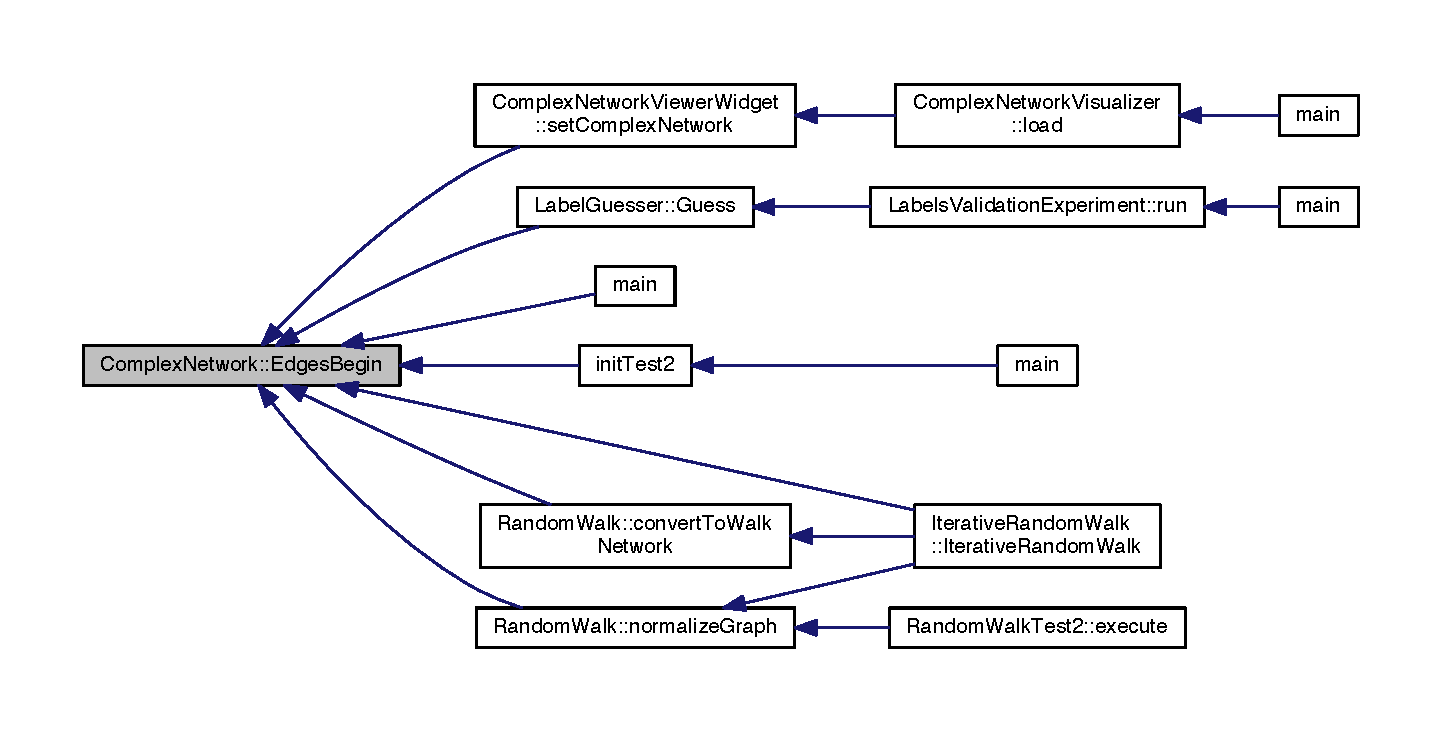
\includegraphics[width=350pt]{class_complex_network_a2167b224079f5c0b44443959ad0b6440_icgraph}
\end{center}
\end{figure}


\hypertarget{class_complex_network_a3a228b9a9497db2b9385deb4eb39f1e1}{\index{Complex\+Network@{Complex\+Network}!Edges\+Begin@{Edges\+Begin}}
\index{Edges\+Begin@{Edges\+Begin}!Complex\+Network@{Complex\+Network}}
\subsubsection[{Edges\+Begin}]{\setlength{\rightskip}{0pt plus 5cm}template$<$typename N\+O\+D\+E\+\_\+\+T\+Y\+P\+E , typename E\+D\+G\+E\+\_\+\+T\+Y\+P\+E $>$ {\bf Complex\+Network}$<$ N\+O\+D\+E\+\_\+\+T\+Y\+P\+E, E\+D\+G\+E\+\_\+\+T\+Y\+P\+E $>$\+::{\bf Edge\+Iterator} {\bf Complex\+Network}$<$ N\+O\+D\+E\+\_\+\+T\+Y\+P\+E, E\+D\+G\+E\+\_\+\+T\+Y\+P\+E $>$\+::Edges\+Begin (
\begin{DoxyParamCaption}
{}
\end{DoxyParamCaption}
)}}\label{class_complex_network_a3a228b9a9497db2b9385deb4eb39f1e1}
\hypertarget{class_complex_network_ad806138ea94ec18ed17f4681ab731208}{\index{Complex\+Network@{Complex\+Network}!Edges\+End@{Edges\+End}}
\index{Edges\+End@{Edges\+End}!Complex\+Network@{Complex\+Network}}
\subsubsection[{Edges\+End}]{\setlength{\rightskip}{0pt plus 5cm}template$<$typename N\+O\+D\+E\+\_\+\+T\+Y\+P\+E , typename E\+D\+G\+E\+\_\+\+T\+Y\+P\+E $>$ {\bf Complex\+Network}$<$ N\+O\+D\+E\+\_\+\+T\+Y\+P\+E, E\+D\+G\+E\+\_\+\+T\+Y\+P\+E $>$\+::{\bf Edge\+Iterator} {\bf Complex\+Network}$<$ N\+O\+D\+E\+\_\+\+T\+Y\+P\+E, E\+D\+G\+E\+\_\+\+T\+Y\+P\+E $>$\+::Edges\+End (
\begin{DoxyParamCaption}
\item[{{\bf node\+\_\+id}}]{node\+\_\+from}
\end{DoxyParamCaption}
)}}\label{class_complex_network_ad806138ea94ec18ed17f4681ab731208}


Here is the caller graph for this function\+:\nopagebreak
\begin{figure}[H]
\begin{center}
\leavevmode
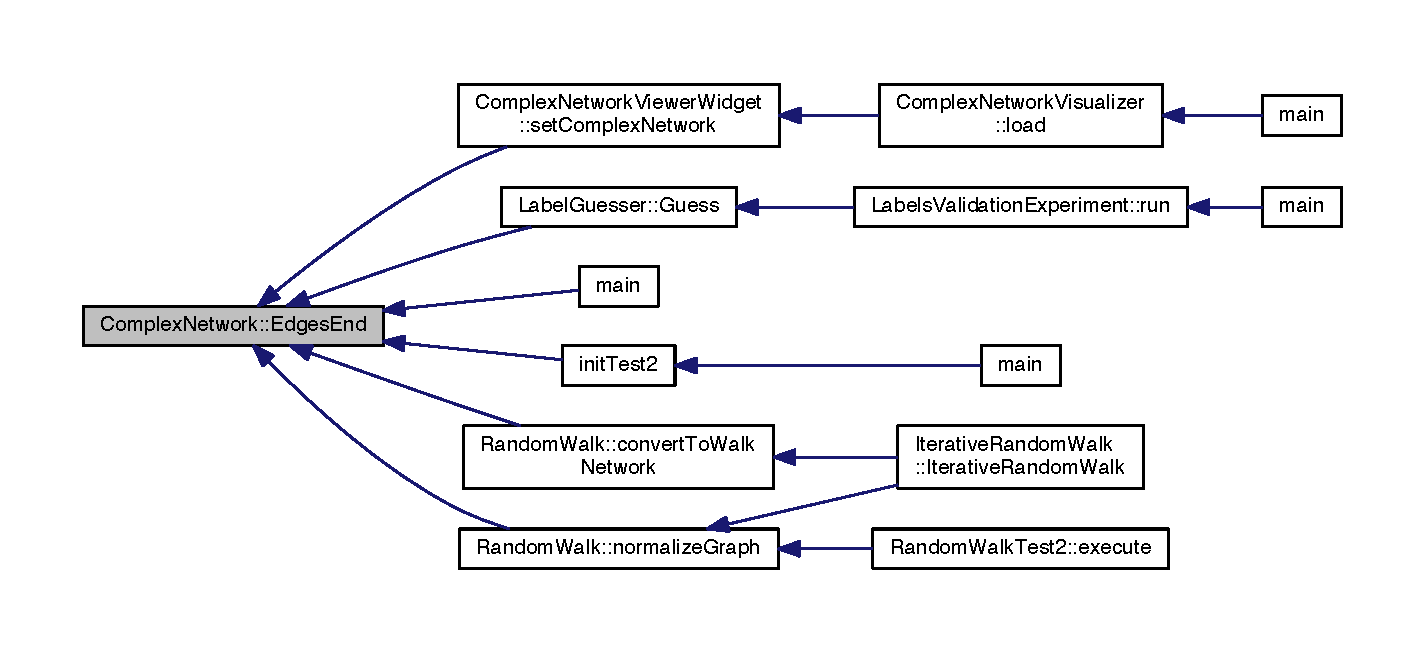
\includegraphics[width=350pt]{class_complex_network_ad806138ea94ec18ed17f4681ab731208_icgraph}
\end{center}
\end{figure}


\hypertarget{class_complex_network_afa7d628b66a815d97afbf5373640d12b}{\index{Complex\+Network@{Complex\+Network}!Edges\+End@{Edges\+End}}
\index{Edges\+End@{Edges\+End}!Complex\+Network@{Complex\+Network}}
\subsubsection[{Edges\+End}]{\setlength{\rightskip}{0pt plus 5cm}template$<$typename N\+O\+D\+E\+\_\+\+T\+Y\+P\+E , typename E\+D\+G\+E\+\_\+\+T\+Y\+P\+E $>$ {\bf Complex\+Network}$<$ N\+O\+D\+E\+\_\+\+T\+Y\+P\+E, E\+D\+G\+E\+\_\+\+T\+Y\+P\+E $>$\+::{\bf Edge\+Iterator} {\bf Complex\+Network}$<$ N\+O\+D\+E\+\_\+\+T\+Y\+P\+E, E\+D\+G\+E\+\_\+\+T\+Y\+P\+E $>$\+::Edges\+End (
\begin{DoxyParamCaption}
{}
\end{DoxyParamCaption}
)}}\label{class_complex_network_afa7d628b66a815d97afbf5373640d12b}
\hypertarget{class_complex_network_a2c90f4efd046776d7a53776b24daae0f}{\index{Complex\+Network@{Complex\+Network}!End@{End}}
\index{End@{End}!Complex\+Network@{Complex\+Network}}
\subsubsection[{End}]{\setlength{\rightskip}{0pt plus 5cm}template$<$typename N\+O\+D\+E\+\_\+\+T\+Y\+P\+E , typename E\+D\+G\+E\+\_\+\+T\+Y\+P\+E $>$ {\bf Complex\+Network}$<$ N\+O\+D\+E\+\_\+\+T\+Y\+P\+E, E\+D\+G\+E\+\_\+\+T\+Y\+P\+E $>$\+::{\bf Node\+Iterator} {\bf Complex\+Network}$<$ N\+O\+D\+E\+\_\+\+T\+Y\+P\+E, E\+D\+G\+E\+\_\+\+T\+Y\+P\+E $>$\+::End (
\begin{DoxyParamCaption}
{}
\end{DoxyParamCaption}
)}}\label{class_complex_network_a2c90f4efd046776d7a53776b24daae0f}


Here is the caller graph for this function\+:
\nopagebreak
\begin{figure}[H]
\begin{center}
\leavevmode
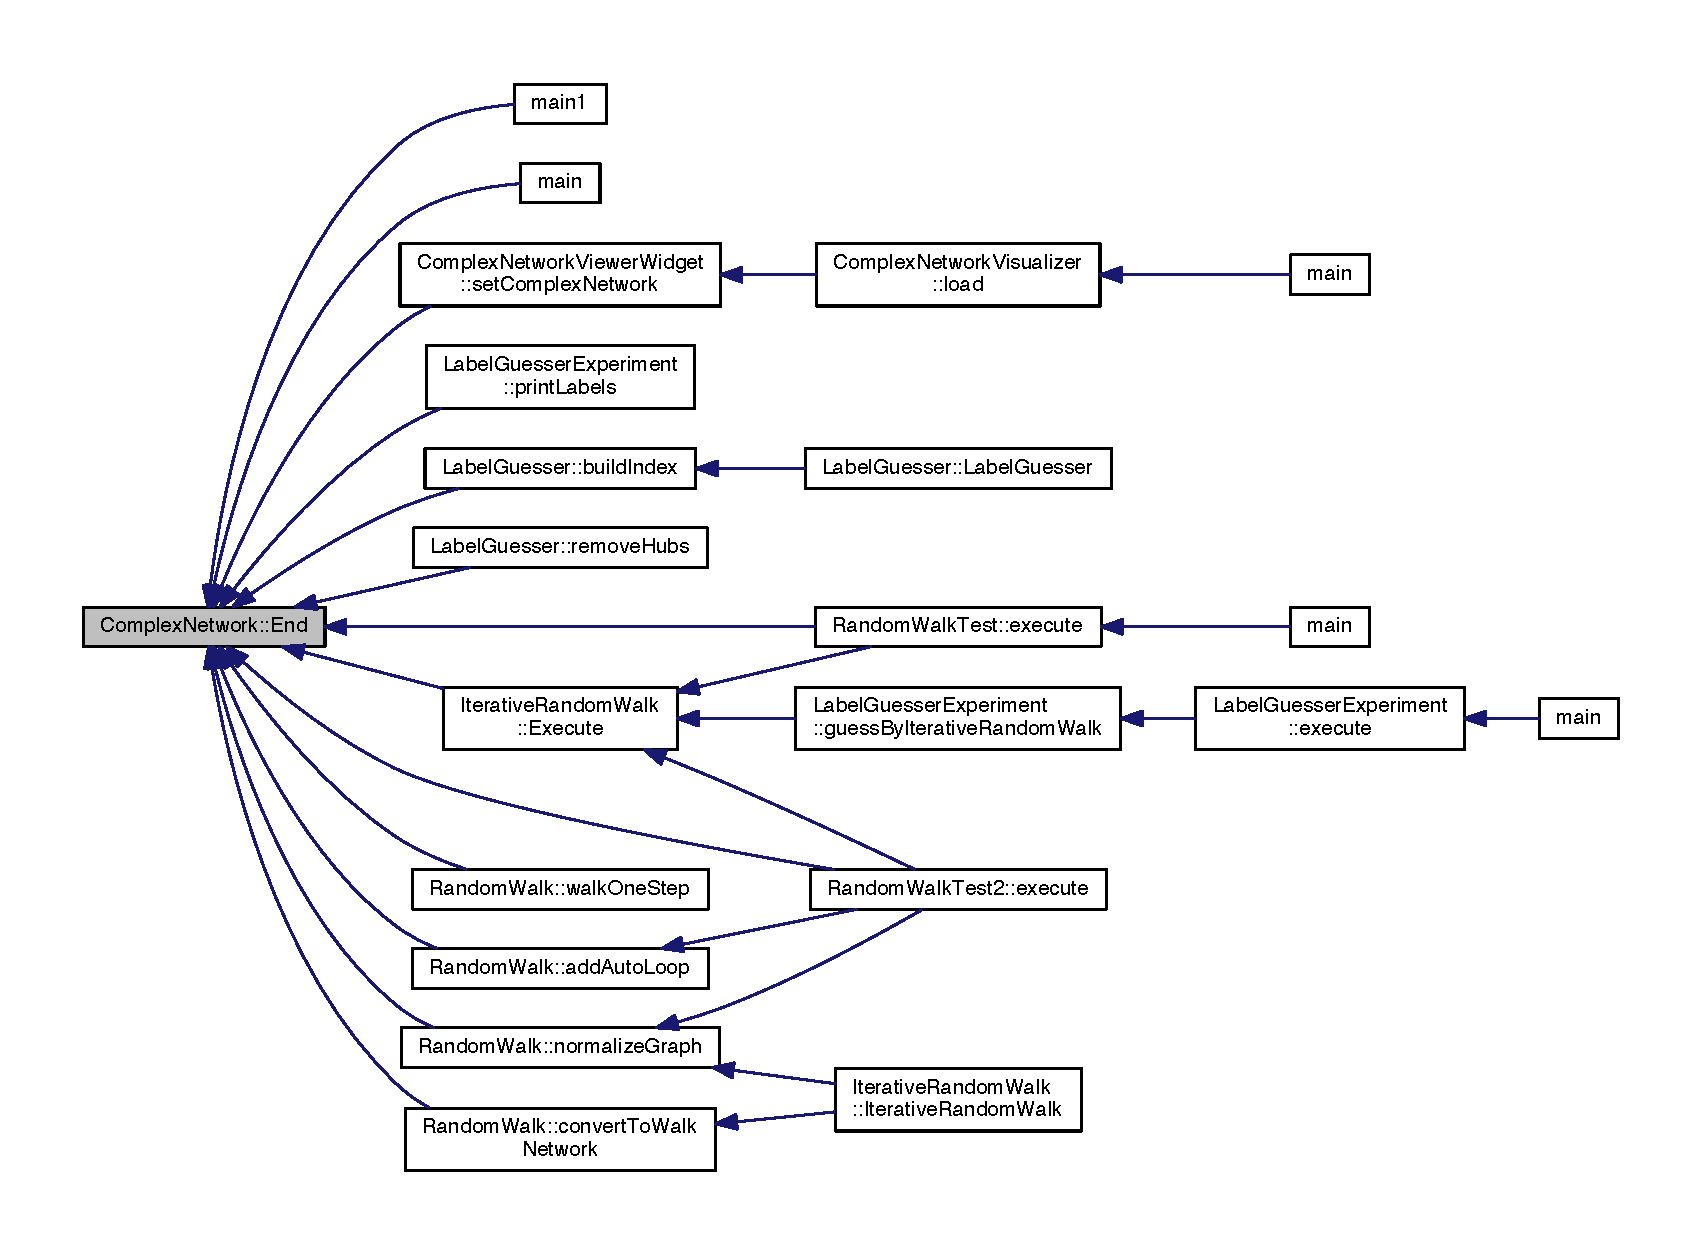
\includegraphics[width=350pt]{class_complex_network_a2c90f4efd046776d7a53776b24daae0f_icgraph}
\end{center}
\end{figure}


\hypertarget{class_complex_network_a6a1c638e4604efe06c12ce3065020ec1}{\index{Complex\+Network@{Complex\+Network}!get\+Edge@{get\+Edge}}
\index{get\+Edge@{get\+Edge}!Complex\+Network@{Complex\+Network}}
\subsubsection[{get\+Edge}]{\setlength{\rightskip}{0pt plus 5cm}template$<$typename N\+O\+D\+E\+\_\+\+T\+Y\+P\+E , typename E\+D\+G\+E\+\_\+\+T\+Y\+P\+E $>$ E\+D\+G\+E\+\_\+\+T\+Y\+P\+E $\ast$ {\bf Complex\+Network}$<$ N\+O\+D\+E\+\_\+\+T\+Y\+P\+E, E\+D\+G\+E\+\_\+\+T\+Y\+P\+E $>$\+::get\+Edge (
\begin{DoxyParamCaption}
\item[{{\bf node\+\_\+id}}]{from, }
\item[{{\bf node\+\_\+id}}]{to}
\end{DoxyParamCaption}
)\hspace{0.3cm}{\ttfamily [virtual]}}}\label{class_complex_network_a6a1c638e4604efe06c12ce3065020ec1}


Here is the caller graph for this function\+:
\nopagebreak
\begin{figure}[H]
\begin{center}
\leavevmode
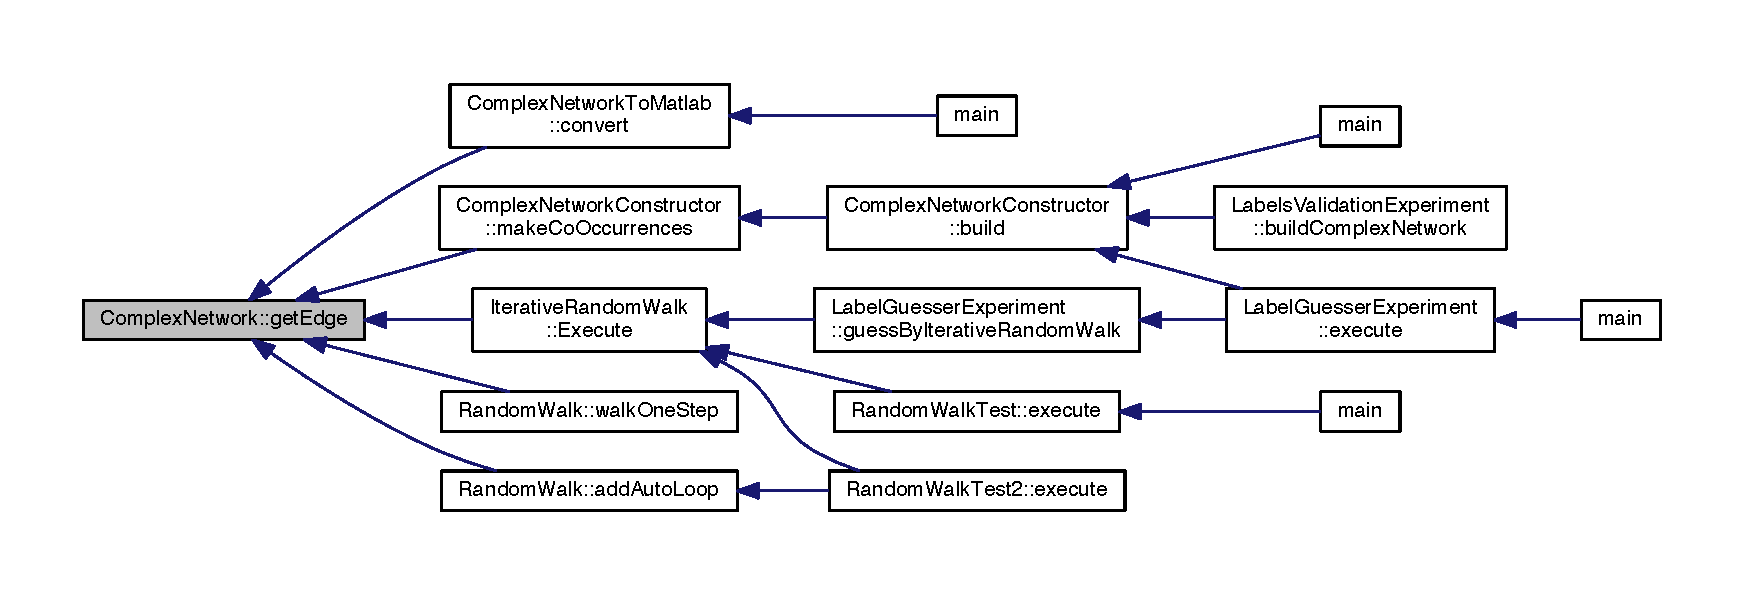
\includegraphics[width=350pt]{class_complex_network_a6a1c638e4604efe06c12ce3065020ec1_icgraph}
\end{center}
\end{figure}


\hypertarget{class_complex_network_ad440008416fc33500754d77b2532560f}{\index{Complex\+Network@{Complex\+Network}!get\+Edge\+From\+Edge\+Id@{get\+Edge\+From\+Edge\+Id}}
\index{get\+Edge\+From\+Edge\+Id@{get\+Edge\+From\+Edge\+Id}!Complex\+Network@{Complex\+Network}}
\subsubsection[{get\+Edge\+From\+Edge\+Id}]{\setlength{\rightskip}{0pt plus 5cm}template$<$typename N\+O\+D\+E\+\_\+\+T\+Y\+P\+E , typename E\+D\+G\+E\+\_\+\+T\+Y\+P\+E $>$ E\+D\+G\+E\+\_\+\+T\+Y\+P\+E $\ast$ {\bf Complex\+Network}$<$ N\+O\+D\+E\+\_\+\+T\+Y\+P\+E, E\+D\+G\+E\+\_\+\+T\+Y\+P\+E $>$\+::get\+Edge\+From\+Edge\+Id (
\begin{DoxyParamCaption}
\item[{{\bf edge\+\_\+id}}]{id}
\end{DoxyParamCaption}
)\hspace{0.3cm}{\ttfamily [virtual]}}}\label{class_complex_network_ad440008416fc33500754d77b2532560f}
\hypertarget{class_complex_network_a3711aff250a942a9ad61d0571be82c43}{\index{Complex\+Network@{Complex\+Network}!get\+Node@{get\+Node}}
\index{get\+Node@{get\+Node}!Complex\+Network@{Complex\+Network}}
\subsubsection[{get\+Node}]{\setlength{\rightskip}{0pt plus 5cm}template$<$typename N\+O\+D\+E\+\_\+\+T\+Y\+P\+E , typename E\+D\+G\+E\+\_\+\+T\+Y\+P\+E $>$ N\+O\+D\+E\+\_\+\+T\+Y\+P\+E $\ast$ {\bf Complex\+Network}$<$ N\+O\+D\+E\+\_\+\+T\+Y\+P\+E, E\+D\+G\+E\+\_\+\+T\+Y\+P\+E $>$\+::get\+Node (
\begin{DoxyParamCaption}
\item[{{\bf node\+\_\+id}}]{id}
\end{DoxyParamCaption}
)\hspace{0.3cm}{\ttfamily [virtual]}}}\label{class_complex_network_a3711aff250a942a9ad61d0571be82c43}


Here is the caller graph for this function\+:
\nopagebreak
\begin{figure}[H]
\begin{center}
\leavevmode
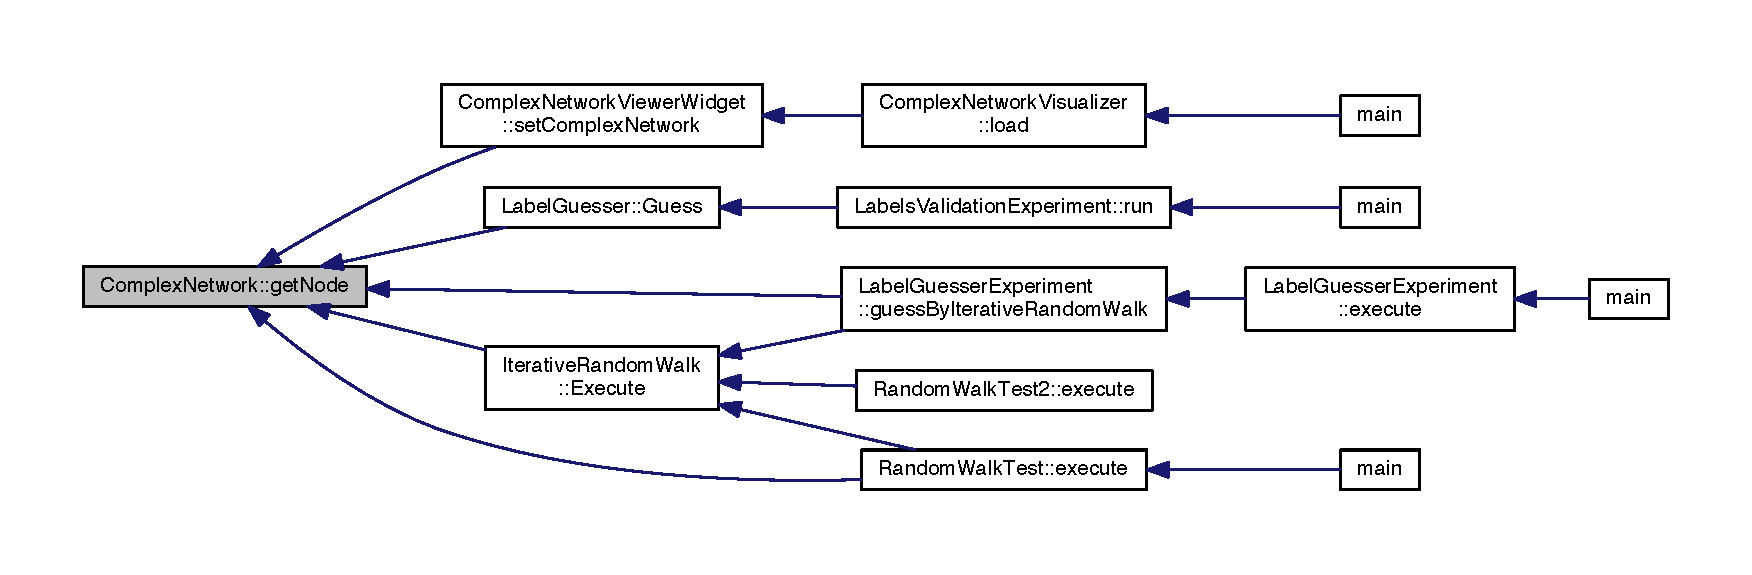
\includegraphics[width=350pt]{class_complex_network_a3711aff250a942a9ad61d0571be82c43_icgraph}
\end{center}
\end{figure}


\hypertarget{class_complex_network_a720cb4e40342648d394792cc693d29a5}{\index{Complex\+Network@{Complex\+Network}!get\+Num\+Edges@{get\+Num\+Edges}}
\index{get\+Num\+Edges@{get\+Num\+Edges}!Complex\+Network@{Complex\+Network}}
\subsubsection[{get\+Num\+Edges}]{\setlength{\rightskip}{0pt plus 5cm}template$<$typename N\+O\+D\+E\+\_\+\+T\+Y\+P\+E , typename E\+D\+G\+E\+\_\+\+T\+Y\+P\+E $>$ unsigned int {\bf Complex\+Network}$<$ N\+O\+D\+E\+\_\+\+T\+Y\+P\+E, E\+D\+G\+E\+\_\+\+T\+Y\+P\+E $>$\+::get\+Num\+Edges (
\begin{DoxyParamCaption}
{}
\end{DoxyParamCaption}
) const}}\label{class_complex_network_a720cb4e40342648d394792cc693d29a5}


Here is the caller graph for this function\+:\nopagebreak
\begin{figure}[H]
\begin{center}
\leavevmode
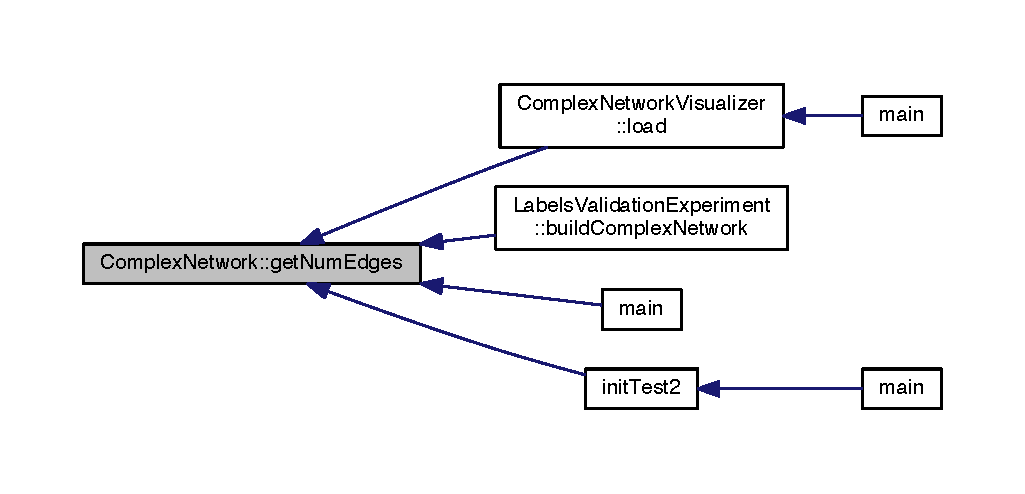
\includegraphics[width=350pt]{class_complex_network_a720cb4e40342648d394792cc693d29a5_icgraph}
\end{center}
\end{figure}


\hypertarget{class_complex_network_a4036d2cda2dc5596d03e164c3455aff6}{\index{Complex\+Network@{Complex\+Network}!get\+Num\+Edges@{get\+Num\+Edges}}
\index{get\+Num\+Edges@{get\+Num\+Edges}!Complex\+Network@{Complex\+Network}}
\subsubsection[{get\+Num\+Edges}]{\setlength{\rightskip}{0pt plus 5cm}template$<$typename N\+O\+D\+E\+\_\+\+T\+Y\+P\+E , typename E\+D\+G\+E\+\_\+\+T\+Y\+P\+E $>$ unsigned int {\bf Complex\+Network}$<$ N\+O\+D\+E\+\_\+\+T\+Y\+P\+E, E\+D\+G\+E\+\_\+\+T\+Y\+P\+E $>$\+::get\+Num\+Edges (
\begin{DoxyParamCaption}
\item[{{\bf node\+\_\+id}}]{id}
\end{DoxyParamCaption}
) const}}\label{class_complex_network_a4036d2cda2dc5596d03e164c3455aff6}
\hypertarget{class_complex_network_afee98f26ceed674c17be01a740787170}{\index{Complex\+Network@{Complex\+Network}!get\+Num\+Nodes@{get\+Num\+Nodes}}
\index{get\+Num\+Nodes@{get\+Num\+Nodes}!Complex\+Network@{Complex\+Network}}
\subsubsection[{get\+Num\+Nodes}]{\setlength{\rightskip}{0pt plus 5cm}template$<$typename N\+O\+D\+E\+\_\+\+T\+Y\+P\+E , typename E\+D\+G\+E\+\_\+\+T\+Y\+P\+E $>$ unsigned int {\bf Complex\+Network}$<$ N\+O\+D\+E\+\_\+\+T\+Y\+P\+E, E\+D\+G\+E\+\_\+\+T\+Y\+P\+E $>$\+::get\+Num\+Nodes (
\begin{DoxyParamCaption}
{}
\end{DoxyParamCaption}
) const}}\label{class_complex_network_afee98f26ceed674c17be01a740787170}


Here is the caller graph for this function\+:
\nopagebreak
\begin{figure}[H]
\begin{center}
\leavevmode
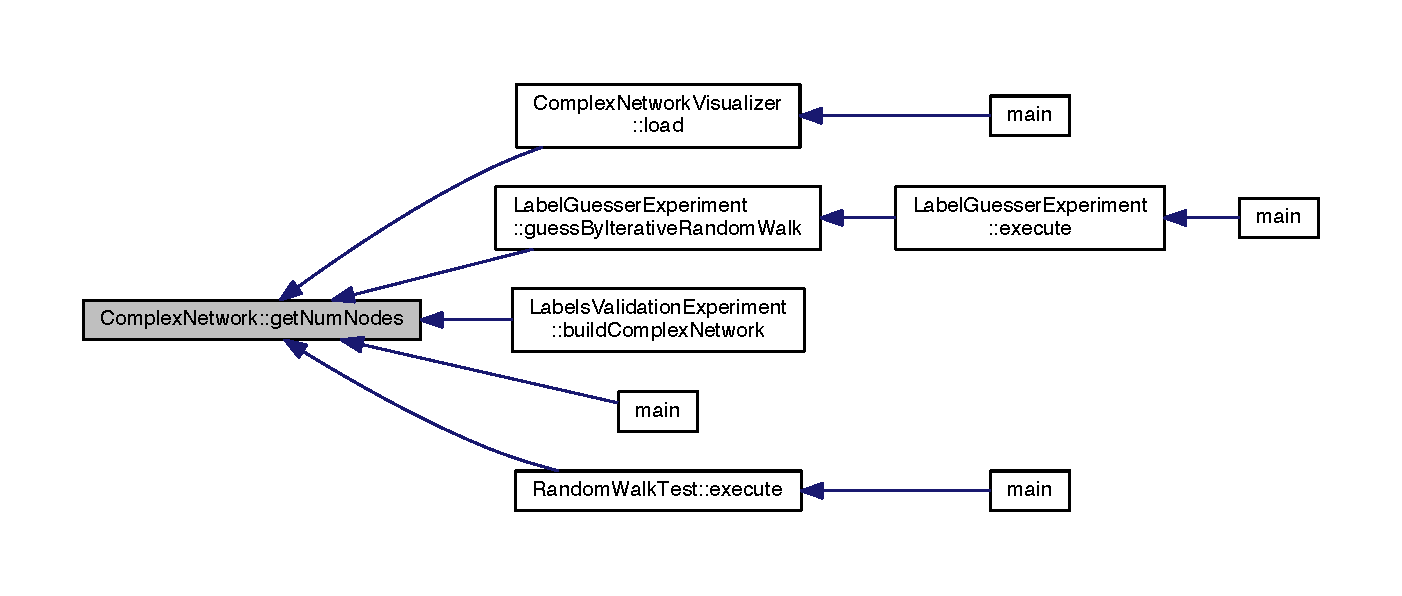
\includegraphics[width=350pt]{class_complex_network_afee98f26ceed674c17be01a740787170_icgraph}
\end{center}
\end{figure}


\hypertarget{class_complex_network_a54fbdb35418f424e8dad0dbc5dc16bee}{\index{Complex\+Network@{Complex\+Network}!load@{load}}
\index{load@{load}!Complex\+Network@{Complex\+Network}}
\subsubsection[{load}]{\setlength{\rightskip}{0pt plus 5cm}template$<$typename N\+O\+D\+E\+\_\+\+T\+Y\+P\+E , typename E\+D\+G\+E\+\_\+\+T\+Y\+P\+E $>$ void {\bf Complex\+Network}$<$ N\+O\+D\+E\+\_\+\+T\+Y\+P\+E, E\+D\+G\+E\+\_\+\+T\+Y\+P\+E $>$\+::load (
\begin{DoxyParamCaption}
\item[{const char $\ast$}]{filename}
\end{DoxyParamCaption}
)}}\label{class_complex_network_a54fbdb35418f424e8dad0dbc5dc16bee}


Here is the caller graph for this function\+:\nopagebreak
\begin{figure}[H]
\begin{center}
\leavevmode
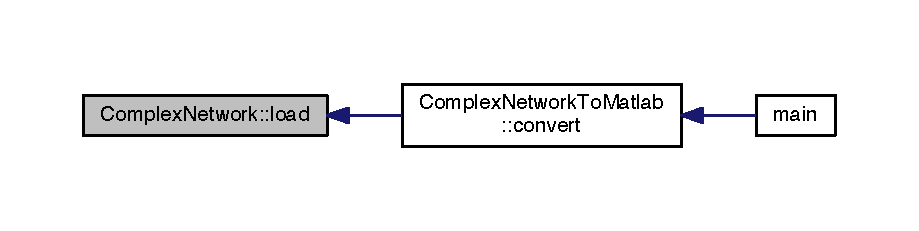
\includegraphics[width=350pt]{class_complex_network_a54fbdb35418f424e8dad0dbc5dc16bee_icgraph}
\end{center}
\end{figure}


\hypertarget{class_complex_network_a5a8b07f5ca5d247e13a2e2bc5ac75de1}{\index{Complex\+Network@{Complex\+Network}!operator=@{operator=}}
\index{operator=@{operator=}!Complex\+Network@{Complex\+Network}}
\subsubsection[{operator=}]{\setlength{\rightskip}{0pt plus 5cm}template$<$typename N\+O\+D\+E\+\_\+\+T\+Y\+P\+E, typename E\+D\+G\+E\+\_\+\+T\+Y\+P\+E$>$ {\bf Complex\+Network}$<$ N\+O\+D\+E\+\_\+\+T\+Y\+P\+E, E\+D\+G\+E\+\_\+\+T\+Y\+P\+E $>$ \& {\bf Complex\+Network}$<$ N\+O\+D\+E\+\_\+\+T\+Y\+P\+E, E\+D\+G\+E\+\_\+\+T\+Y\+P\+E $>$\+::operator= (
\begin{DoxyParamCaption}
\item[{const {\bf Complex\+Network}$<$ N\+O\+D\+E\+\_\+\+T\+Y\+P\+E, E\+D\+G\+E\+\_\+\+T\+Y\+P\+E $>$ \&}]{cn}
\end{DoxyParamCaption}
)}}\label{class_complex_network_a5a8b07f5ca5d247e13a2e2bc5ac75de1}
\hypertarget{class_complex_network_a9b2c7df561a2ad5fc14b04a5c5c56828}{\index{Complex\+Network@{Complex\+Network}!remove\+Edge@{remove\+Edge}}
\index{remove\+Edge@{remove\+Edge}!Complex\+Network@{Complex\+Network}}
\subsubsection[{remove\+Edge}]{\setlength{\rightskip}{0pt plus 5cm}template$<$typename N\+O\+D\+E\+\_\+\+T\+Y\+P\+E , typename E\+D\+G\+E\+\_\+\+T\+Y\+P\+E $>$ bool {\bf Complex\+Network}$<$ N\+O\+D\+E\+\_\+\+T\+Y\+P\+E, E\+D\+G\+E\+\_\+\+T\+Y\+P\+E $>$\+::remove\+Edge (
\begin{DoxyParamCaption}
\item[{{\bf node\+\_\+id}}]{from, }
\item[{{\bf node\+\_\+id}}]{to}
\end{DoxyParamCaption}
)\hspace{0.3cm}{\ttfamily [virtual]}}}\label{class_complex_network_a9b2c7df561a2ad5fc14b04a5c5c56828}


Here is the caller graph for this function\+:\nopagebreak
\begin{figure}[H]
\begin{center}
\leavevmode
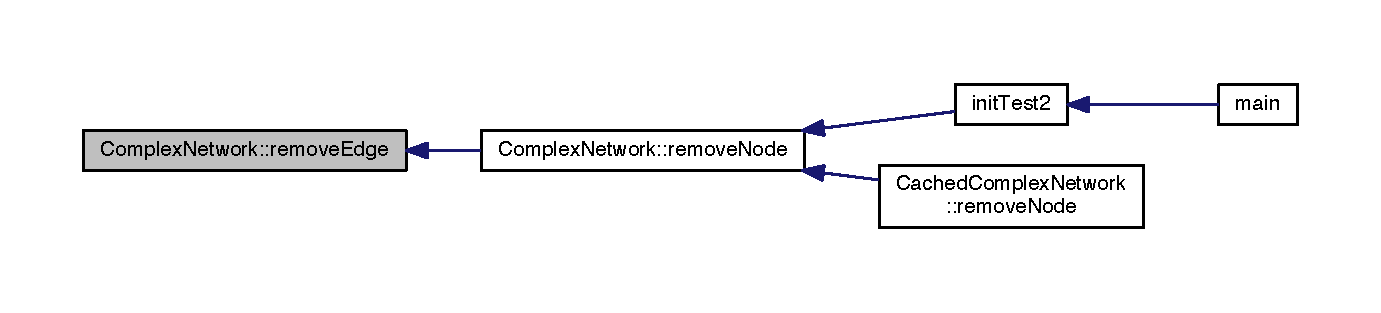
\includegraphics[width=350pt]{class_complex_network_a9b2c7df561a2ad5fc14b04a5c5c56828_icgraph}
\end{center}
\end{figure}


\hypertarget{class_complex_network_a33f2b4528cc31296ede98be7e6dcd600}{\index{Complex\+Network@{Complex\+Network}!remove\+Node@{remove\+Node}}
\index{remove\+Node@{remove\+Node}!Complex\+Network@{Complex\+Network}}
\subsubsection[{remove\+Node}]{\setlength{\rightskip}{0pt plus 5cm}template$<$typename N\+O\+D\+E\+\_\+\+T\+Y\+P\+E , typename E\+D\+G\+E\+\_\+\+T\+Y\+P\+E $>$ bool {\bf Complex\+Network}$<$ N\+O\+D\+E\+\_\+\+T\+Y\+P\+E, E\+D\+G\+E\+\_\+\+T\+Y\+P\+E $>$\+::remove\+Node (
\begin{DoxyParamCaption}
\item[{{\bf node\+\_\+id}}]{id}
\end{DoxyParamCaption}
)\hspace{0.3cm}{\ttfamily [virtual]}}}\label{class_complex_network_a33f2b4528cc31296ede98be7e6dcd600}


Reimplemented in \hyperlink{class_cached_complex_network_a800aa02b94aa4bb73227e139cb246ddf}{Cached\+Complex\+Network$<$ N\+O\+D\+E\+\_\+\+T\+Y\+P\+E, E\+D\+G\+E\+\_\+\+T\+Y\+P\+E $>$}, and \hyperlink{class_cached_complex_network_a800aa02b94aa4bb73227e139cb246ddf}{Cached\+Complex\+Network$<$ int, double $>$}.



Here is the call graph for this function\+:\nopagebreak
\begin{figure}[H]
\begin{center}
\leavevmode
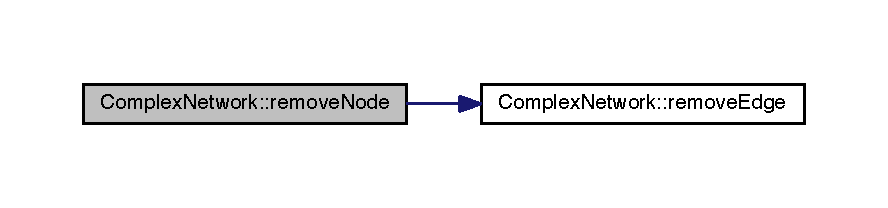
\includegraphics[width=350pt]{class_complex_network_a33f2b4528cc31296ede98be7e6dcd600_cgraph}
\end{center}
\end{figure}




Here is the caller graph for this function\+:\nopagebreak
\begin{figure}[H]
\begin{center}
\leavevmode
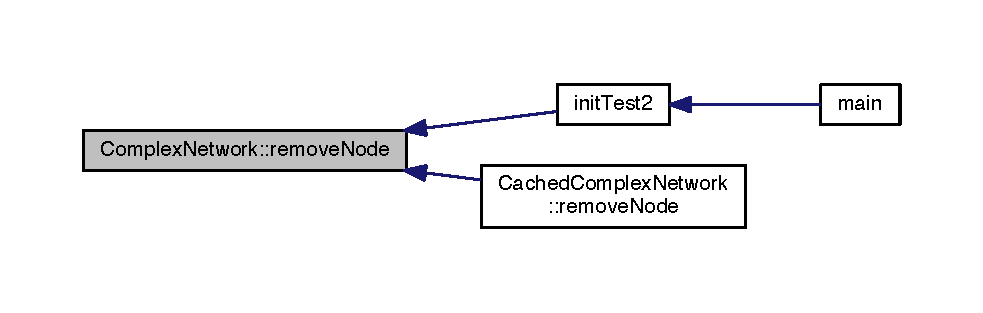
\includegraphics[width=350pt]{class_complex_network_a33f2b4528cc31296ede98be7e6dcd600_icgraph}
\end{center}
\end{figure}


\hypertarget{class_complex_network_a5d127d4296808b7ccdadccaa58084e96}{\index{Complex\+Network@{Complex\+Network}!save@{save}}
\index{save@{save}!Complex\+Network@{Complex\+Network}}
\subsubsection[{save}]{\setlength{\rightskip}{0pt plus 5cm}template$<$typename N\+O\+D\+E\+\_\+\+T\+Y\+P\+E , typename E\+D\+G\+E\+\_\+\+T\+Y\+P\+E $>$ void {\bf Complex\+Network}$<$ N\+O\+D\+E\+\_\+\+T\+Y\+P\+E, E\+D\+G\+E\+\_\+\+T\+Y\+P\+E $>$\+::save (
\begin{DoxyParamCaption}
\item[{const char $\ast$}]{filename}
\end{DoxyParamCaption}
)}}\label{class_complex_network_a5d127d4296808b7ccdadccaa58084e96}


Here is the caller graph for this function\+:\nopagebreak
\begin{figure}[H]
\begin{center}
\leavevmode
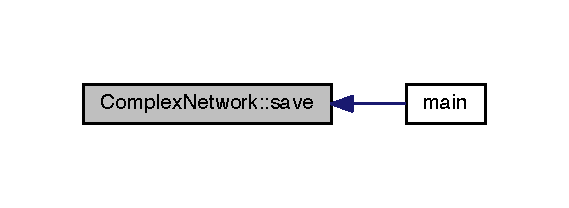
\includegraphics[width=273pt]{class_complex_network_a5d127d4296808b7ccdadccaa58084e96_icgraph}
\end{center}
\end{figure}




\subsection{Member Data Documentation}
\hypertarget{class_complex_network_a5305dba65a6d949064e46a6729c39e53}{\index{Complex\+Network@{Complex\+Network}!current\+\_\+edge\+\_\+id@{current\+\_\+edge\+\_\+id}}
\index{current\+\_\+edge\+\_\+id@{current\+\_\+edge\+\_\+id}!Complex\+Network@{Complex\+Network}}
\subsubsection[{current\+\_\+edge\+\_\+id}]{\setlength{\rightskip}{0pt plus 5cm}template$<$typename N\+O\+D\+E\+\_\+\+T\+Y\+P\+E, typename E\+D\+G\+E\+\_\+\+T\+Y\+P\+E$>$ {\bf edge\+\_\+id} {\bf Complex\+Network}$<$ N\+O\+D\+E\+\_\+\+T\+Y\+P\+E, E\+D\+G\+E\+\_\+\+T\+Y\+P\+E $>$\+::current\+\_\+edge\+\_\+id\hspace{0.3cm}{\ttfamily [protected]}}}\label{class_complex_network_a5305dba65a6d949064e46a6729c39e53}
\hypertarget{class_complex_network_ab71dc127e36a989049df28f58f2c315a}{\index{Complex\+Network@{Complex\+Network}!current\+\_\+node\+\_\+id@{current\+\_\+node\+\_\+id}}
\index{current\+\_\+node\+\_\+id@{current\+\_\+node\+\_\+id}!Complex\+Network@{Complex\+Network}}
\subsubsection[{current\+\_\+node\+\_\+id}]{\setlength{\rightskip}{0pt plus 5cm}template$<$typename N\+O\+D\+E\+\_\+\+T\+Y\+P\+E, typename E\+D\+G\+E\+\_\+\+T\+Y\+P\+E$>$ {\bf node\+\_\+id} {\bf Complex\+Network}$<$ N\+O\+D\+E\+\_\+\+T\+Y\+P\+E, E\+D\+G\+E\+\_\+\+T\+Y\+P\+E $>$\+::current\+\_\+node\+\_\+id\hspace{0.3cm}{\ttfamily [protected]}}}\label{class_complex_network_ab71dc127e36a989049df28f58f2c315a}
\hypertarget{class_complex_network_abc2c2def62701d56ec56c8b0accbedb9}{\index{Complex\+Network@{Complex\+Network}!description@{description}}
\index{description@{description}!Complex\+Network@{Complex\+Network}}
\subsubsection[{description}]{\setlength{\rightskip}{0pt plus 5cm}template$<$typename N\+O\+D\+E\+\_\+\+T\+Y\+P\+E, typename E\+D\+G\+E\+\_\+\+T\+Y\+P\+E$>$ char {\bf Complex\+Network}$<$ N\+O\+D\+E\+\_\+\+T\+Y\+P\+E, E\+D\+G\+E\+\_\+\+T\+Y\+P\+E $>$\+::description\mbox{[}200\mbox{]}}}\label{class_complex_network_abc2c2def62701d56ec56c8b0accbedb9}
\hypertarget{class_complex_network_ae1f8a32f89d84aab42475d8fe46dfa09}{\index{Complex\+Network@{Complex\+Network}!directed@{directed}}
\index{directed@{directed}!Complex\+Network@{Complex\+Network}}
\subsubsection[{directed}]{\setlength{\rightskip}{0pt plus 5cm}template$<$typename N\+O\+D\+E\+\_\+\+T\+Y\+P\+E, typename E\+D\+G\+E\+\_\+\+T\+Y\+P\+E$>$ bool {\bf Complex\+Network}$<$ N\+O\+D\+E\+\_\+\+T\+Y\+P\+E, E\+D\+G\+E\+\_\+\+T\+Y\+P\+E $>$\+::directed\hspace{0.3cm}{\ttfamily [protected]}}}\label{class_complex_network_ae1f8a32f89d84aab42475d8fe46dfa09}
\hypertarget{class_complex_network_a666bb7ad7f5ab90416f037aeb1ba11d0}{\index{Complex\+Network@{Complex\+Network}!edge@{edge}}
\index{edge@{edge}!Complex\+Network@{Complex\+Network}}
\subsubsection[{edge}]{\setlength{\rightskip}{0pt plus 5cm}template$<$typename N\+O\+D\+E\+\_\+\+T\+Y\+P\+E, typename E\+D\+G\+E\+\_\+\+T\+Y\+P\+E$>$ Q\+Hash$<$ {\bf edge\+\_\+id}, E\+D\+G\+E\+\_\+\+T\+Y\+P\+E$>$ {\bf Complex\+Network}$<$ N\+O\+D\+E\+\_\+\+T\+Y\+P\+E, E\+D\+G\+E\+\_\+\+T\+Y\+P\+E $>$\+::edge\hspace{0.3cm}{\ttfamily [protected]}}}\label{class_complex_network_a666bb7ad7f5ab90416f037aeb1ba11d0}
\hypertarget{class_complex_network_adbdf613ffde926399cd5f6e7b8c09536}{\index{Complex\+Network@{Complex\+Network}!edges@{edges}}
\index{edges@{edges}!Complex\+Network@{Complex\+Network}}
\subsubsection[{edges}]{\setlength{\rightskip}{0pt plus 5cm}template$<$typename N\+O\+D\+E\+\_\+\+T\+Y\+P\+E, typename E\+D\+G\+E\+\_\+\+T\+Y\+P\+E$>$ Q\+Hash$<$ {\bf node\+\_\+id}, Q\+Hash$<${\bf node\+\_\+id}, {\bf edge\+\_\+id}$>$ $>$ {\bf Complex\+Network}$<$ N\+O\+D\+E\+\_\+\+T\+Y\+P\+E, E\+D\+G\+E\+\_\+\+T\+Y\+P\+E $>$\+::edges\hspace{0.3cm}{\ttfamily [protected]}}}\label{class_complex_network_adbdf613ffde926399cd5f6e7b8c09536}
\hypertarget{class_complex_network_ab9ab3dbbbcd8dd173ec40938391c0fc4}{\index{Complex\+Network@{Complex\+Network}!file\+\_\+header@{file\+\_\+header}}
\index{file\+\_\+header@{file\+\_\+header}!Complex\+Network@{Complex\+Network}}
\subsubsection[{file\+\_\+header}]{\setlength{\rightskip}{0pt plus 5cm}struct \{ ... \}  {\bf Complex\+Network}$<$ N\+O\+D\+E\+\_\+\+T\+Y\+P\+E, E\+D\+G\+E\+\_\+\+T\+Y\+P\+E $>$\+::file\+\_\+header\hspace{0.3cm}{\ttfamily [protected]}}}\label{class_complex_network_ab9ab3dbbbcd8dd173ec40938391c0fc4}
\hypertarget{class_complex_network_a6b0ecc57af689b9ba9f8855132d1c275}{\index{Complex\+Network@{Complex\+Network}!nodes@{nodes}}
\index{nodes@{nodes}!Complex\+Network@{Complex\+Network}}
\subsubsection[{nodes}]{\setlength{\rightskip}{0pt plus 5cm}template$<$typename N\+O\+D\+E\+\_\+\+T\+Y\+P\+E, typename E\+D\+G\+E\+\_\+\+T\+Y\+P\+E$>$ Q\+Hash$<$ {\bf node\+\_\+id}, N\+O\+D\+E\+\_\+\+T\+Y\+P\+E$>$ {\bf Complex\+Network}$<$ N\+O\+D\+E\+\_\+\+T\+Y\+P\+E, E\+D\+G\+E\+\_\+\+T\+Y\+P\+E $>$\+::nodes\hspace{0.3cm}{\ttfamily [protected]}}}\label{class_complex_network_a6b0ecc57af689b9ba9f8855132d1c275}
\hypertarget{class_complex_network_ac4a7f179af0187eb3071969642b445cc}{\index{Complex\+Network@{Complex\+Network}!num\+\_\+edges@{num\+\_\+edges}}
\index{num\+\_\+edges@{num\+\_\+edges}!Complex\+Network@{Complex\+Network}}
\subsubsection[{num\+\_\+edges}]{\setlength{\rightskip}{0pt plus 5cm}template$<$typename N\+O\+D\+E\+\_\+\+T\+Y\+P\+E, typename E\+D\+G\+E\+\_\+\+T\+Y\+P\+E$>$ unsigned int {\bf Complex\+Network}$<$ N\+O\+D\+E\+\_\+\+T\+Y\+P\+E, E\+D\+G\+E\+\_\+\+T\+Y\+P\+E $>$\+::num\+\_\+edges}}\label{class_complex_network_ac4a7f179af0187eb3071969642b445cc}
\hypertarget{class_complex_network_a6c8777ba48e68c02d2d523abe904b6b1}{\index{Complex\+Network@{Complex\+Network}!num\+\_\+nodes@{num\+\_\+nodes}}
\index{num\+\_\+nodes@{num\+\_\+nodes}!Complex\+Network@{Complex\+Network}}
\subsubsection[{num\+\_\+nodes}]{\setlength{\rightskip}{0pt plus 5cm}template$<$typename N\+O\+D\+E\+\_\+\+T\+Y\+P\+E, typename E\+D\+G\+E\+\_\+\+T\+Y\+P\+E$>$ unsigned int {\bf Complex\+Network}$<$ N\+O\+D\+E\+\_\+\+T\+Y\+P\+E, E\+D\+G\+E\+\_\+\+T\+Y\+P\+E $>$\+::num\+\_\+nodes}}\label{class_complex_network_a6c8777ba48e68c02d2d523abe904b6b1}


The documentation for this class was generated from the following file\+:\begin{DoxyCompactItemize}
\item 
Sources/\+Complex\+Network/\hyperlink{_complex_network_8hpp}{Complex\+Network.\+hpp}\end{DoxyCompactItemize}

\hypertarget{class_complex_network_constructor}{\section{Complex\+Network\+Constructor Class Reference}
\label{class_complex_network_constructor}\index{Complex\+Network\+Constructor@{Complex\+Network\+Constructor}}
}


{\ttfamily \#include $<$Complex\+Network\+Constructor.\+hpp$>$}

\subsection*{Public Member Functions}
\begin{DoxyCompactItemize}
\item 
\hyperlink{class_complex_network_constructor_afe14ec2655225f646877381c87b86df3}{Complex\+Network\+Constructor} (\hyperlink{class_features_complex_network}{Features\+Complex\+Network} \&\hyperlink{class_complex_network_constructor_aa099456a58edc5c1885323061206b3e6}{cn}, \hyperlink{class_database_reader}{Database\+Reader} \&\hyperlink{class_complex_network_constructor_ad223ad7e464ff159d91a89deb4e943cc}{reader}, Q\+List$<$ \hyperlink{class_feature_factory_abstract}{Feature\+Factory\+Abstract} $\ast$ $>$ \hyperlink{class_complex_network_constructor_ae79b538a8b9253cd71de5fef1be1c18a}{extractors})
\item 
void \hyperlink{class_complex_network_constructor_a19d313488e2c19172e362b521f53e329}{build} ()
\end{DoxyCompactItemize}
\subsection*{Private Member Functions}
\begin{DoxyCompactItemize}
\item 
void \hyperlink{class_complex_network_constructor_aa41263b4bf0e157d451652d772f84ef7}{make\+Co\+Occurrences} (Q\+Linked\+List$<$ \hyperlink{class_feature_abstract}{Feature\+Abstract} $\ast$ $>$ \&features, Q\+List$<$ int $>$ \&regions\+Ids)
\item 
float \hyperlink{class_complex_network_constructor_a8c4875120270d689a5fd08e47a6b4b59}{recorrencia} (float \hyperlink{class_complex_network_constructor_afc016404ca7dda4b05807e3ca004c308}{time})
\end{DoxyCompactItemize}
\subsection*{Private Attributes}
\begin{DoxyCompactItemize}
\item 
Q\+Hash$<$ \hyperlink{class_feature_abstract_key}{Feature\+Abstract\+Key}, \\*
\hyperlink{_complex_network_8hpp_a8323334ca788fde39682469321590d52}{node\+\_\+id} $>$ \hyperlink{class_complex_network_constructor_ad616573ee07edff462c552d3fc2bfce7}{index}
\item 
\hyperlink{class_features_complex_network}{Features\+Complex\+Network} \& \hyperlink{class_complex_network_constructor_aa099456a58edc5c1885323061206b3e6}{cn}
\item 
\hyperlink{class_database_reader}{Database\+Reader} \& \hyperlink{class_complex_network_constructor_ad223ad7e464ff159d91a89deb4e943cc}{reader}
\item 
Q\+List$<$ \hyperlink{class_feature_factory_abstract}{Feature\+Factory\+Abstract} $\ast$ $>$ \hyperlink{class_complex_network_constructor_ae79b538a8b9253cd71de5fef1be1c18a}{extractors}
\item 
unsigned long long int \hyperlink{class_complex_network_constructor_afc016404ca7dda4b05807e3ca004c308}{time} =1
\item 
float \hyperlink{class_complex_network_constructor_a9d3e346719dc1f8f3093a48b8d44e669}{lambda} =80
\item 
float \hyperlink{class_complex_network_constructor_aa7fe374b9733338b8176708f77d29c55}{learning\+Rate} =0.\+3
\end{DoxyCompactItemize}


Collaboration diagram for Complex\+Network\+Constructor\+:\nopagebreak
\begin{figure}[H]
\begin{center}
\leavevmode
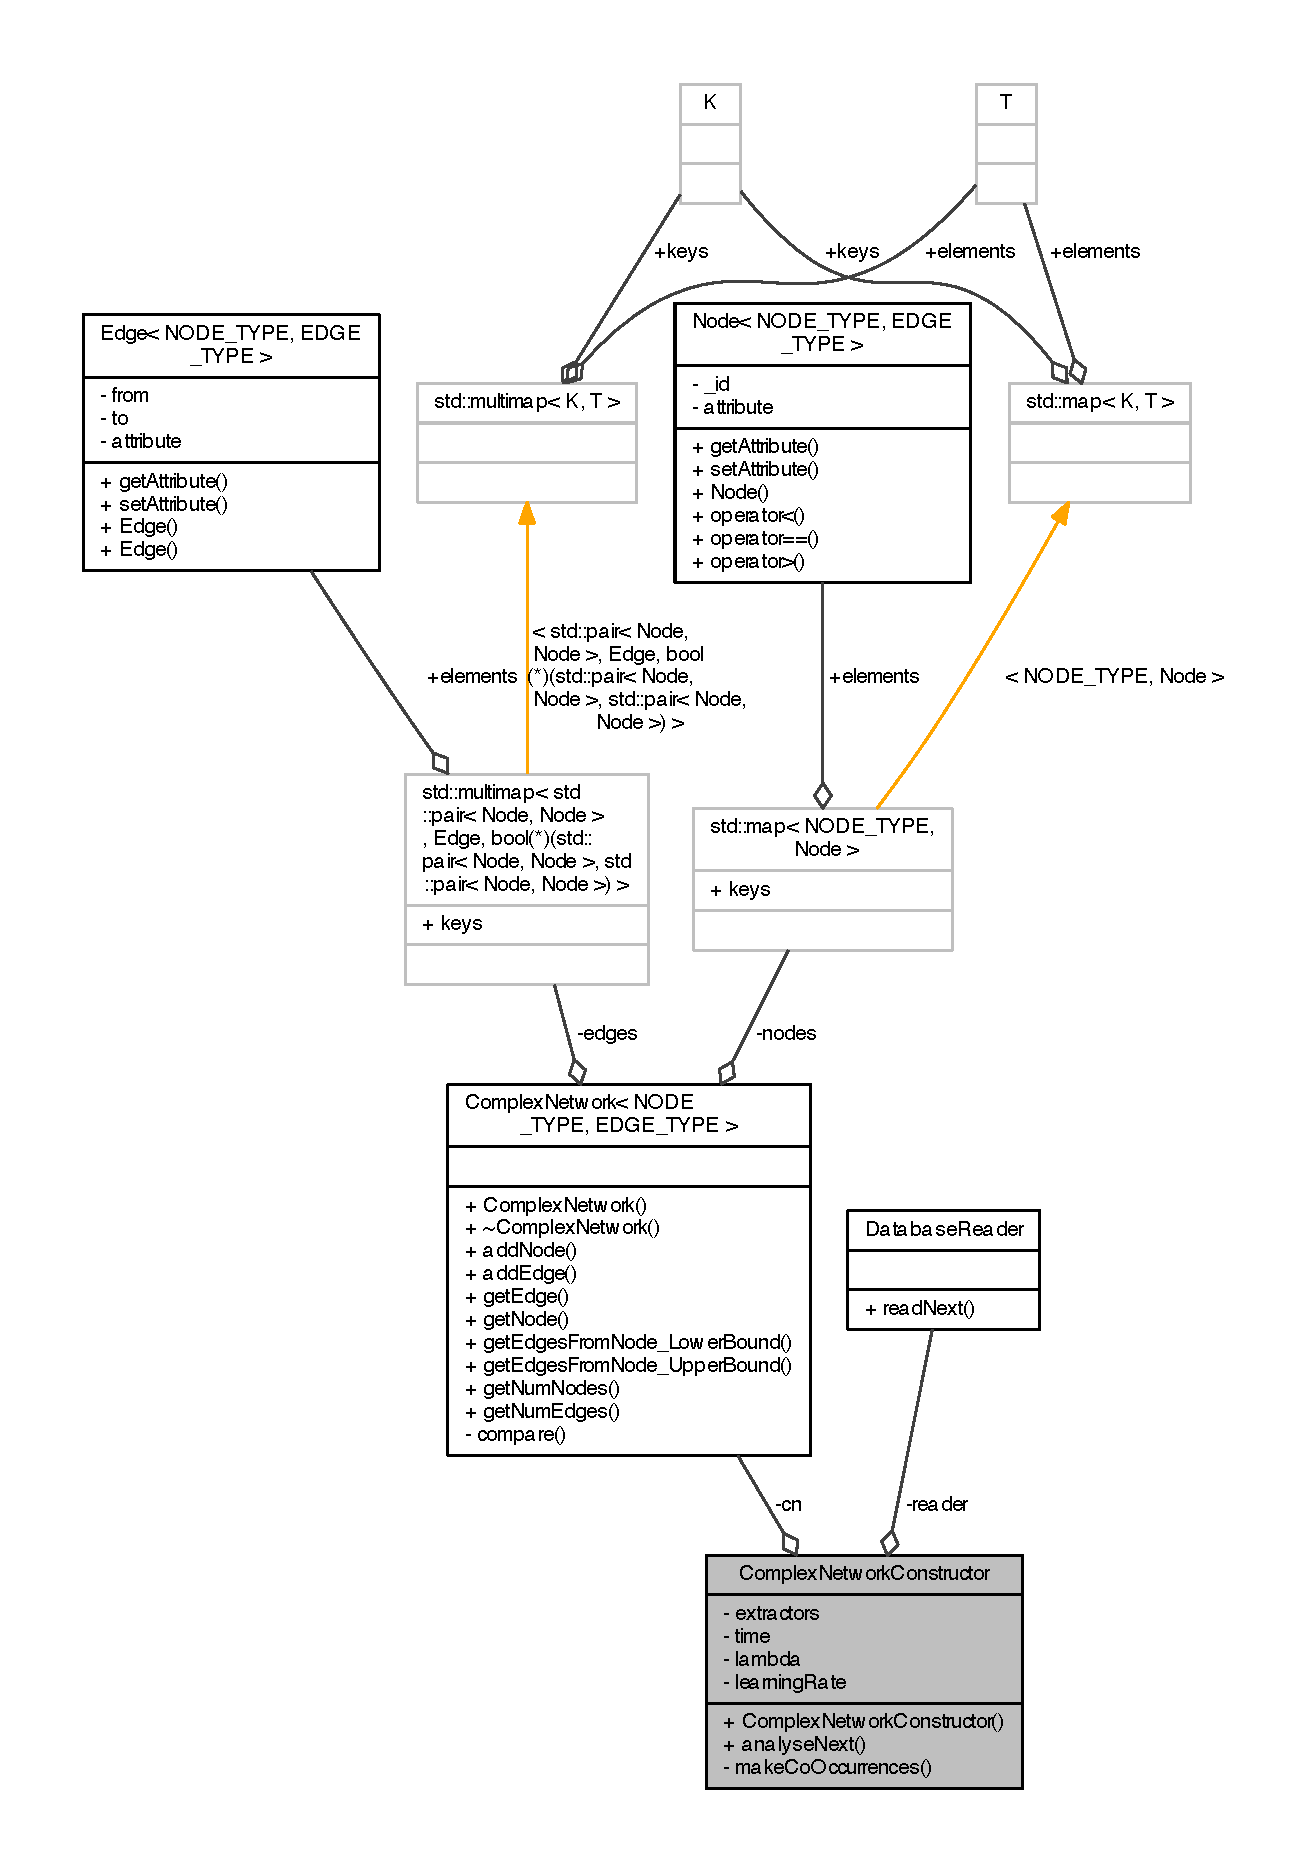
\includegraphics[width=350pt]{class_complex_network_constructor__coll__graph}
\end{center}
\end{figure}


\subsection{Constructor \& Destructor Documentation}
\hypertarget{class_complex_network_constructor_afe14ec2655225f646877381c87b86df3}{\index{Complex\+Network\+Constructor@{Complex\+Network\+Constructor}!Complex\+Network\+Constructor@{Complex\+Network\+Constructor}}
\index{Complex\+Network\+Constructor@{Complex\+Network\+Constructor}!Complex\+Network\+Constructor@{Complex\+Network\+Constructor}}
\subsubsection[{Complex\+Network\+Constructor}]{\setlength{\rightskip}{0pt plus 5cm}Complex\+Network\+Constructor\+::\+Complex\+Network\+Constructor (
\begin{DoxyParamCaption}
\item[{{\bf Features\+Complex\+Network} \&}]{cn, }
\item[{{\bf Database\+Reader} \&}]{reader, }
\item[{Q\+List$<$ {\bf Feature\+Factory\+Abstract} $\ast$ $>$}]{extractors}
\end{DoxyParamCaption}
)}}\label{class_complex_network_constructor_afe14ec2655225f646877381c87b86df3}


\subsection{Member Function Documentation}
\hypertarget{class_complex_network_constructor_a19d313488e2c19172e362b521f53e329}{\index{Complex\+Network\+Constructor@{Complex\+Network\+Constructor}!build@{build}}
\index{build@{build}!Complex\+Network\+Constructor@{Complex\+Network\+Constructor}}
\subsubsection[{build}]{\setlength{\rightskip}{0pt plus 5cm}void Complex\+Network\+Constructor\+::build (
\begin{DoxyParamCaption}
{}
\end{DoxyParamCaption}
)}}\label{class_complex_network_constructor_a19d313488e2c19172e362b521f53e329}


Here is the call graph for this function\+:\nopagebreak
\begin{figure}[H]
\begin{center}
\leavevmode
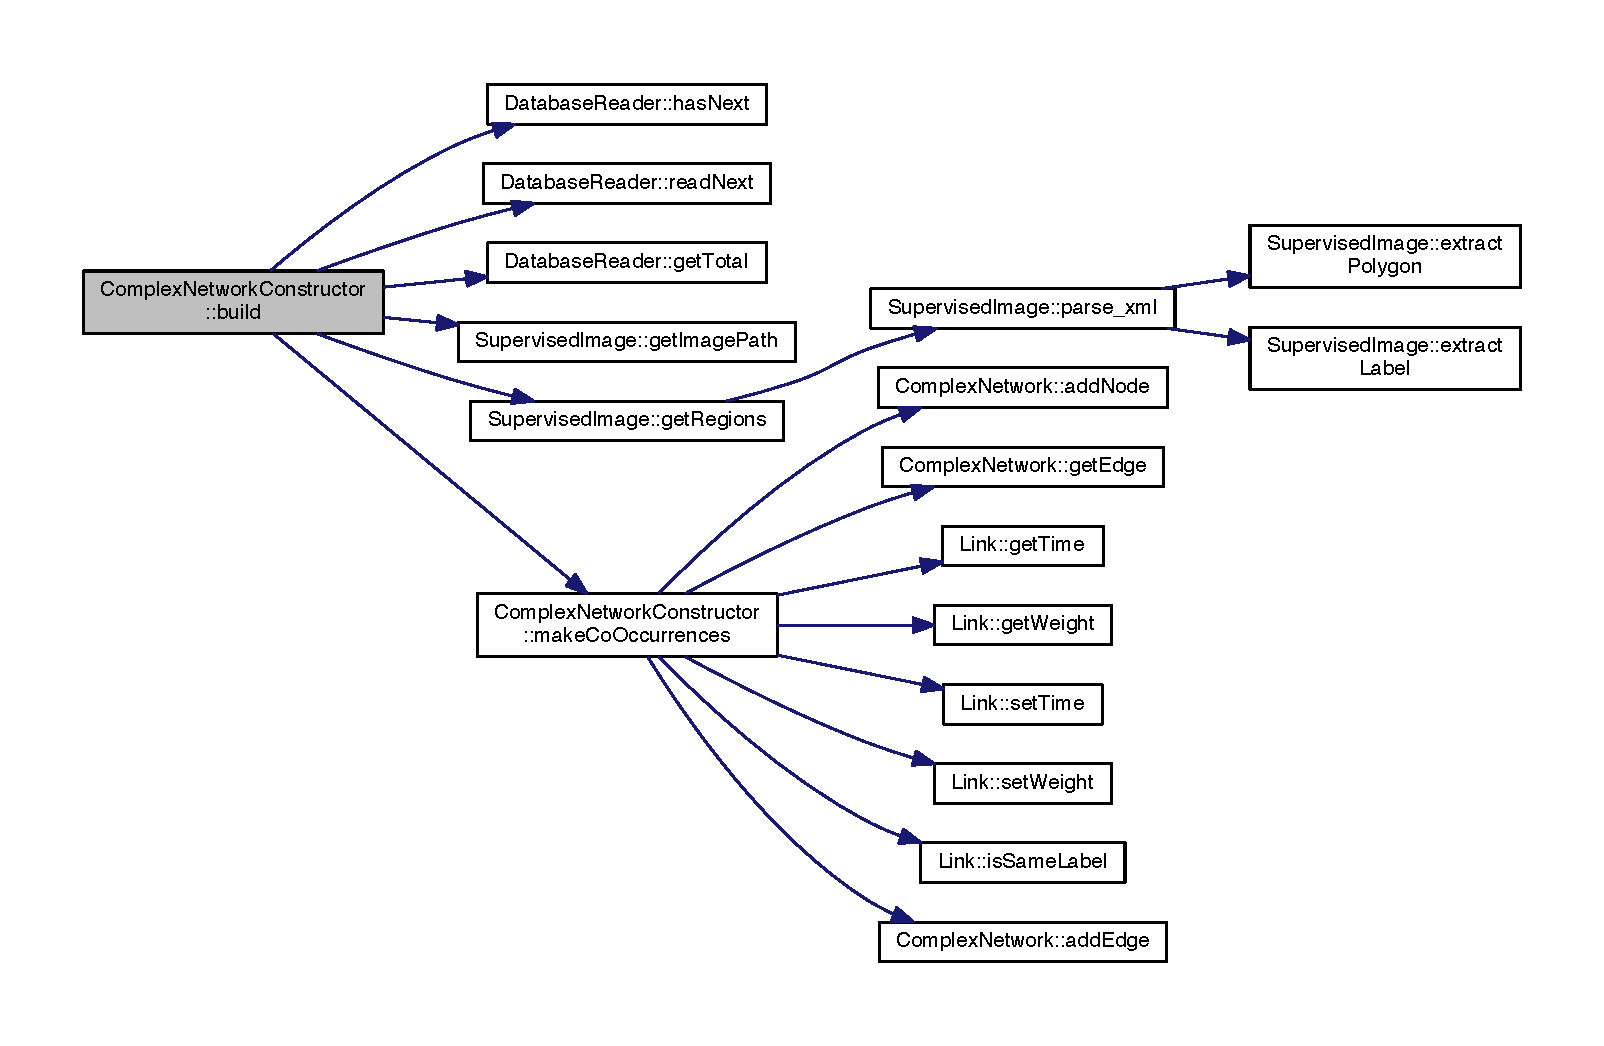
\includegraphics[width=350pt]{class_complex_network_constructor_a19d313488e2c19172e362b521f53e329_cgraph}
\end{center}
\end{figure}




Here is the caller graph for this function\+:
\nopagebreak
\begin{figure}[H]
\begin{center}
\leavevmode
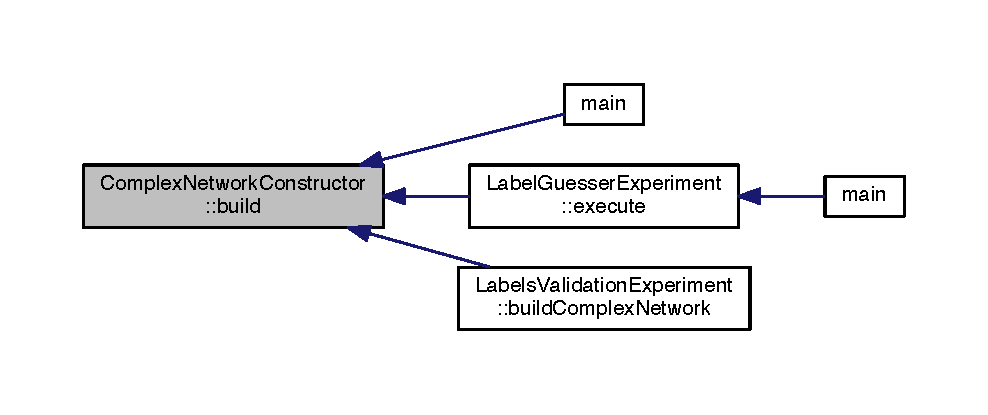
\includegraphics[width=350pt]{class_complex_network_constructor_a19d313488e2c19172e362b521f53e329_icgraph}
\end{center}
\end{figure}


\hypertarget{class_complex_network_constructor_aa41263b4bf0e157d451652d772f84ef7}{\index{Complex\+Network\+Constructor@{Complex\+Network\+Constructor}!make\+Co\+Occurrences@{make\+Co\+Occurrences}}
\index{make\+Co\+Occurrences@{make\+Co\+Occurrences}!Complex\+Network\+Constructor@{Complex\+Network\+Constructor}}
\subsubsection[{make\+Co\+Occurrences}]{\setlength{\rightskip}{0pt plus 5cm}void Complex\+Network\+Constructor\+::make\+Co\+Occurrences (
\begin{DoxyParamCaption}
\item[{Q\+Linked\+List$<$ {\bf Feature\+Abstract} $\ast$ $>$ \&}]{features, }
\item[{Q\+List$<$ int $>$ \&}]{regions\+Ids}
\end{DoxyParamCaption}
)\hspace{0.3cm}{\ttfamily [private]}}}\label{class_complex_network_constructor_aa41263b4bf0e157d451652d772f84ef7}
Atualiza os pesos as arestas de acordo com a Equação\+: \[ w_{i,j} = w_{i,j} + \alpha\left(\frac{\lambda}{\Delta t} - w_{i,j} \right) \] 

Here is the call graph for this function\+:\nopagebreak
\begin{figure}[H]
\begin{center}
\leavevmode
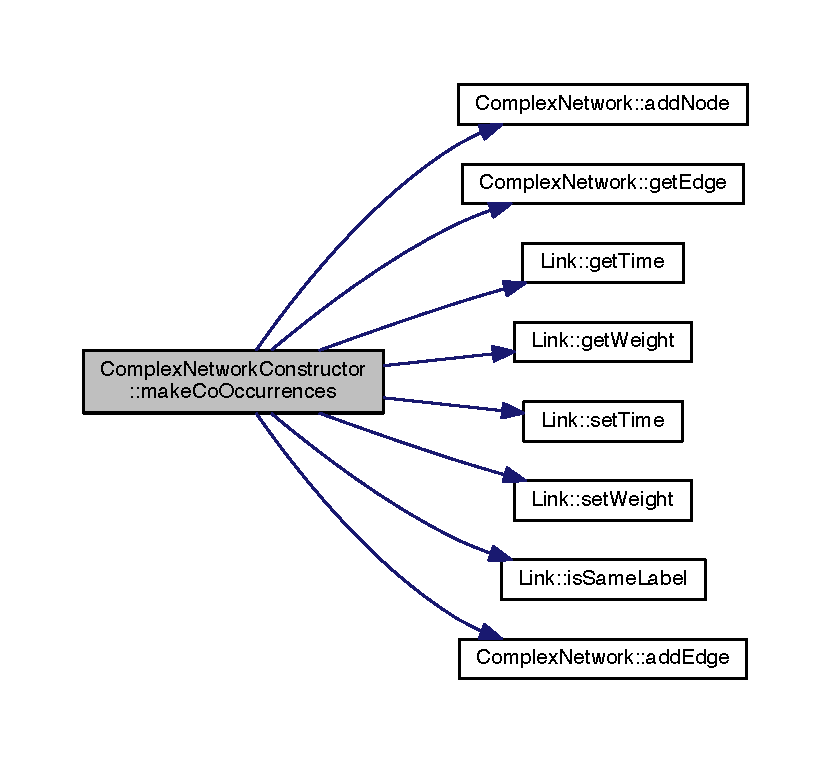
\includegraphics[width=350pt]{class_complex_network_constructor_aa41263b4bf0e157d451652d772f84ef7_cgraph}
\end{center}
\end{figure}




Here is the caller graph for this function\+:
\nopagebreak
\begin{figure}[H]
\begin{center}
\leavevmode
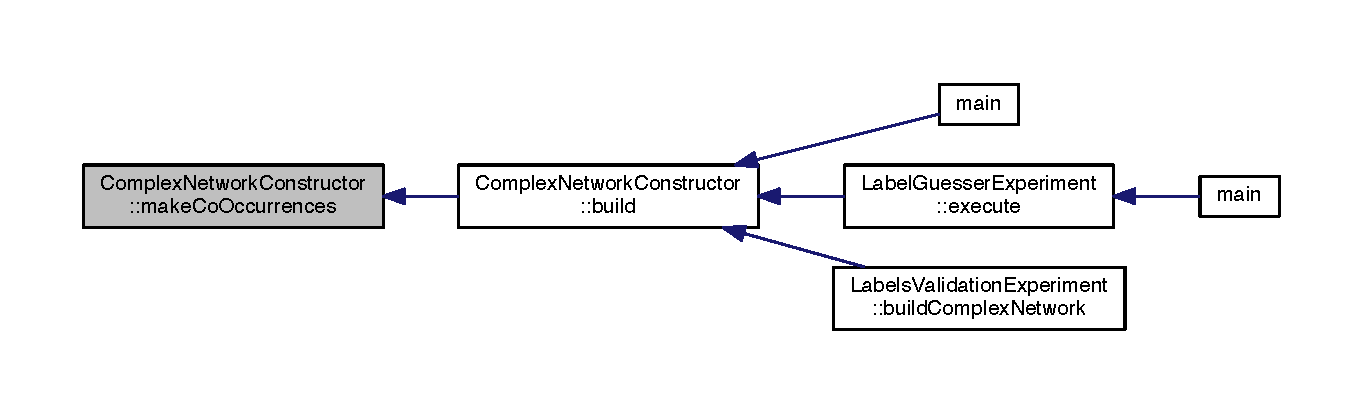
\includegraphics[width=350pt]{class_complex_network_constructor_aa41263b4bf0e157d451652d772f84ef7_icgraph}
\end{center}
\end{figure}


\hypertarget{class_complex_network_constructor_a8c4875120270d689a5fd08e47a6b4b59}{\index{Complex\+Network\+Constructor@{Complex\+Network\+Constructor}!recorrencia@{recorrencia}}
\index{recorrencia@{recorrencia}!Complex\+Network\+Constructor@{Complex\+Network\+Constructor}}
\subsubsection[{recorrencia}]{\setlength{\rightskip}{0pt plus 5cm}float Complex\+Network\+Constructor\+::recorrencia (
\begin{DoxyParamCaption}
\item[{float}]{time}
\end{DoxyParamCaption}
)\hspace{0.3cm}{\ttfamily [private]}}}\label{class_complex_network_constructor_a8c4875120270d689a5fd08e47a6b4b59}


\subsection{Member Data Documentation}
\hypertarget{class_complex_network_constructor_aa099456a58edc5c1885323061206b3e6}{\index{Complex\+Network\+Constructor@{Complex\+Network\+Constructor}!cn@{cn}}
\index{cn@{cn}!Complex\+Network\+Constructor@{Complex\+Network\+Constructor}}
\subsubsection[{cn}]{\setlength{\rightskip}{0pt plus 5cm}{\bf Features\+Complex\+Network}\& Complex\+Network\+Constructor\+::cn\hspace{0.3cm}{\ttfamily [private]}}}\label{class_complex_network_constructor_aa099456a58edc5c1885323061206b3e6}
\hypertarget{class_complex_network_constructor_ae79b538a8b9253cd71de5fef1be1c18a}{\index{Complex\+Network\+Constructor@{Complex\+Network\+Constructor}!extractors@{extractors}}
\index{extractors@{extractors}!Complex\+Network\+Constructor@{Complex\+Network\+Constructor}}
\subsubsection[{extractors}]{\setlength{\rightskip}{0pt plus 5cm}Q\+List$<${\bf Feature\+Factory\+Abstract}$\ast$$>$ Complex\+Network\+Constructor\+::extractors\hspace{0.3cm}{\ttfamily [private]}}}\label{class_complex_network_constructor_ae79b538a8b9253cd71de5fef1be1c18a}
\hypertarget{class_complex_network_constructor_ad616573ee07edff462c552d3fc2bfce7}{\index{Complex\+Network\+Constructor@{Complex\+Network\+Constructor}!index@{index}}
\index{index@{index}!Complex\+Network\+Constructor@{Complex\+Network\+Constructor}}
\subsubsection[{index}]{\setlength{\rightskip}{0pt plus 5cm}Q\+Hash$<${\bf Feature\+Abstract\+Key} , {\bf node\+\_\+id}$>$ Complex\+Network\+Constructor\+::index\hspace{0.3cm}{\ttfamily [private]}}}\label{class_complex_network_constructor_ad616573ee07edff462c552d3fc2bfce7}
\hypertarget{class_complex_network_constructor_a9d3e346719dc1f8f3093a48b8d44e669}{\index{Complex\+Network\+Constructor@{Complex\+Network\+Constructor}!lambda@{lambda}}
\index{lambda@{lambda}!Complex\+Network\+Constructor@{Complex\+Network\+Constructor}}
\subsubsection[{lambda}]{\setlength{\rightskip}{0pt plus 5cm}float Complex\+Network\+Constructor\+::lambda =80\hspace{0.3cm}{\ttfamily [private]}}}\label{class_complex_network_constructor_a9d3e346719dc1f8f3093a48b8d44e669}
Esta é a influência do tempo na aprendizagem $ \lambda $ \hypertarget{class_complex_network_constructor_aa7fe374b9733338b8176708f77d29c55}{\index{Complex\+Network\+Constructor@{Complex\+Network\+Constructor}!learning\+Rate@{learning\+Rate}}
\index{learning\+Rate@{learning\+Rate}!Complex\+Network\+Constructor@{Complex\+Network\+Constructor}}
\subsubsection[{learning\+Rate}]{\setlength{\rightskip}{0pt plus 5cm}float Complex\+Network\+Constructor\+::learning\+Rate =0.\+3\hspace{0.3cm}{\ttfamily [private]}}}\label{class_complex_network_constructor_aa7fe374b9733338b8176708f77d29c55}
Esta é a taxa de aprendizagem $ \alpha $ \hypertarget{class_complex_network_constructor_ad223ad7e464ff159d91a89deb4e943cc}{\index{Complex\+Network\+Constructor@{Complex\+Network\+Constructor}!reader@{reader}}
\index{reader@{reader}!Complex\+Network\+Constructor@{Complex\+Network\+Constructor}}
\subsubsection[{reader}]{\setlength{\rightskip}{0pt plus 5cm}{\bf Database\+Reader}\& Complex\+Network\+Constructor\+::reader\hspace{0.3cm}{\ttfamily [private]}}}\label{class_complex_network_constructor_ad223ad7e464ff159d91a89deb4e943cc}
\hypertarget{class_complex_network_constructor_afc016404ca7dda4b05807e3ca004c308}{\index{Complex\+Network\+Constructor@{Complex\+Network\+Constructor}!time@{time}}
\index{time@{time}!Complex\+Network\+Constructor@{Complex\+Network\+Constructor}}
\subsubsection[{time}]{\setlength{\rightskip}{0pt plus 5cm}unsigned long long int Complex\+Network\+Constructor\+::time =1\hspace{0.3cm}{\ttfamily [private]}}}\label{class_complex_network_constructor_afc016404ca7dda4b05807e3ca004c308}


The documentation for this class was generated from the following files\+:\begin{DoxyCompactItemize}
\item 
Sources/\+Utilities/\hyperlink{_complex_network_constructor_8hpp}{Complex\+Network\+Constructor.\+hpp}\item 
Sources/\+Utilities/\hyperlink{_complex_network_constructor_8cpp}{Complex\+Network\+Constructor.\+cpp}\end{DoxyCompactItemize}

\hypertarget{class_complex_network_to_matlab}{\section{Complex\+Network\+To\+Matlab Class Reference}
\label{class_complex_network_to_matlab}\index{Complex\+Network\+To\+Matlab@{Complex\+Network\+To\+Matlab}}
}


{\ttfamily \#include $<$Complex\+Network\+To\+Matlab.\+hpp$>$}

\subsection*{Static Public Member Functions}
\begin{DoxyCompactItemize}
\item 
static void \hyperlink{class_complex_network_to_matlab_a8d0d921690e8d376364c733c45c0f777}{convert} (Q\+String input\+File, Q\+String output\+File)
\end{DoxyCompactItemize}


Collaboration diagram for Complex\+Network\+To\+Matlab\+:\nopagebreak
\begin{figure}[H]
\begin{center}
\leavevmode
\includegraphics[width=214pt]{class_complex_network_to_matlab__coll__graph}
\end{center}
\end{figure}


\subsection{Member Function Documentation}
\hypertarget{class_complex_network_to_matlab_a8d0d921690e8d376364c733c45c0f777}{\index{Complex\+Network\+To\+Matlab@{Complex\+Network\+To\+Matlab}!convert@{convert}}
\index{convert@{convert}!Complex\+Network\+To\+Matlab@{Complex\+Network\+To\+Matlab}}
\subsubsection[{convert}]{\setlength{\rightskip}{0pt plus 5cm}static void Complex\+Network\+To\+Matlab\+::convert (
\begin{DoxyParamCaption}
\item[{Q\+String}]{input\+File, }
\item[{Q\+String}]{output\+File}
\end{DoxyParamCaption}
)\hspace{0.3cm}{\ttfamily [inline]}, {\ttfamily [static]}}}\label{class_complex_network_to_matlab_a8d0d921690e8d376364c733c45c0f777}


Here is the caller graph for this function\+:\nopagebreak
\begin{figure}[H]
\begin{center}
\leavevmode
\includegraphics[width=288pt]{class_complex_network_to_matlab_a8d0d921690e8d376364c733c45c0f777_icgraph}
\end{center}
\end{figure}




The documentation for this class was generated from the following file\+:\begin{DoxyCompactItemize}
\item 
Sources/\+Experiments/\+Complex\+Network\+To\+Matlab\+File/\hyperlink{_complex_network_to_matlab_8hpp}{Complex\+Network\+To\+Matlab.\+hpp}\end{DoxyCompactItemize}

\hypertarget{class_complex_network_v2}{\section{Complex\+Network\+V2$<$ N, E $>$ Class Template Reference}
\label{class_complex_network_v2}\index{Complex\+Network\+V2$<$ N, E $>$@{Complex\+Network\+V2$<$ N, E $>$}}
}


{\ttfamily \#include $<$Complex\+Network\+V2.\+hpp$>$}

\subsection*{Classes}
\begin{DoxyCompactItemize}
\item 
class \hyperlink{class_complex_network_v2_1_1_edge_iterator}{Edge\+Iterator}
\item 
class \hyperlink{class_complex_network_v2_1_1_node_iterator}{Node\+Iterator}
\end{DoxyCompactItemize}
\subsection*{Public Member Functions}
\begin{DoxyCompactItemize}
\item 
\hyperlink{class_complex_network_v2_ad0bc60844e1006779e826217958f9eb3}{Complex\+Network\+V2} (bool directed=true)
\item 
virtual \hyperlink{_complex_network_v2_8hpp_a8323334ca788fde39682469321590d52}{node\+\_\+id} \hyperlink{class_complex_network_v2_ac63bea705ca74ac77cee3344e3f9609e}{add\+Node} (const N \&\hyperlink{print_report_8m_aeab71244afb687f16d8c4f5ee9d6ef0e}{n})
\item 
virtual N $\ast$ \hyperlink{class_complex_network_v2_a608da16787ef57d7ae965e33ffa87469}{get\+Node} (\hyperlink{_complex_network_v2_8hpp_a8323334ca788fde39682469321590d52}{node\+\_\+id} id)
\item 
virtual bool \hyperlink{class_complex_network_v2_a8b1b3944a3e616e722322575a6a6562b}{remove\+Node} (\hyperlink{_complex_network_v2_8hpp_a8323334ca788fde39682469321590d52}{node\+\_\+id} id)
\item 
virtual void \hyperlink{class_complex_network_v2_ac846f08c3e92c642aa887801adee6aec}{add\+Edge} (\hyperlink{_complex_network_v2_8hpp_a8323334ca788fde39682469321590d52}{node\+\_\+id} from, \hyperlink{_complex_network_v2_8hpp_a8323334ca788fde39682469321590d52}{node\+\_\+id} to, const E \&e)
\item 
virtual E $\ast$ \hyperlink{class_complex_network_v2_a8eb2185022509ed813a330a9c90897b8}{get\+Edge} (\hyperlink{_complex_network_v2_8hpp_a8323334ca788fde39682469321590d52}{node\+\_\+id} from, \hyperlink{_complex_network_v2_8hpp_a8323334ca788fde39682469321590d52}{node\+\_\+id} to)
\item 
virtual E $\ast$ \hyperlink{class_complex_network_v2_a2379e544ee9681a2003504eb5630e3a3}{get\+Edge\+From\+Edge\+Id} (\hyperlink{_complex_network_v2_8hpp_ad7d18d7b90a45b6625704e92d10aa3a0}{edge\+\_\+id} id)
\item 
virtual bool \hyperlink{class_complex_network_v2_ab35860c7516d18a06d08ca926d24d49d}{remove\+Edge} (\hyperlink{_complex_network_v2_8hpp_a8323334ca788fde39682469321590d52}{node\+\_\+id} from, \hyperlink{_complex_network_v2_8hpp_a8323334ca788fde39682469321590d52}{node\+\_\+id} to)
\item 
virtual void \hyperlink{class_complex_network_v2_a85ae14174dbd7f18e652495dea73e5fe}{clear} ()
\item 
unsigned int \hyperlink{class_complex_network_v2_a62d987623c1335d7b93b3f00e266e576}{get\+Num\+Nodes} () const 
\item 
unsigned int \hyperlink{class_complex_network_v2_ae434858a60a9dde2227c596ff000e5df}{get\+Num\+Edges} () const 
\item 
\hyperlink{class_complex_network_v2_1_1_node_iterator}{Node\+Iterator} \hyperlink{class_complex_network_v2_ad7bfe6bd62d583f42f541f959ecc05f5}{Begin} ()
\item 
\hyperlink{class_complex_network_v2_1_1_node_iterator}{Node\+Iterator} \hyperlink{class_complex_network_v2_a3a82c4a7d3579015eaf4a0c064ff7738}{End} ()
\end{DoxyCompactItemize}
\subsection*{Private Attributes}
\begin{DoxyCompactItemize}
\item 
vector$<$ vector$<$ unique\+\_\+ptr$<$ E $>$ $>$ $>$ \hyperlink{class_complex_network_v2_acc11e6426cbfd381b54ee764dd6846df}{edges}
\item 
vector$<$ unique\+\_\+ptr$<$ N $>$ $>$ \hyperlink{class_complex_network_v2_a8b02e8553951e064475a31e5e01c9186}{nodes}
\end{DoxyCompactItemize}


Collaboration diagram for Complex\+Network\+V2$<$ N, E $>$\+:\nopagebreak
\begin{figure}[H]
\begin{center}
\leavevmode
\includegraphics[height=550pt]{class_complex_network_v2__coll__graph}
\end{center}
\end{figure}


\subsection{Constructor \& Destructor Documentation}
\hypertarget{class_complex_network_v2_ad0bc60844e1006779e826217958f9eb3}{\index{Complex\+Network\+V2@{Complex\+Network\+V2}!Complex\+Network\+V2@{Complex\+Network\+V2}}
\index{Complex\+Network\+V2@{Complex\+Network\+V2}!Complex\+Network\+V2@{Complex\+Network\+V2}}
\subsubsection[{Complex\+Network\+V2}]{\setlength{\rightskip}{0pt plus 5cm}template$<$typename N , typename E $>$ {\bf Complex\+Network\+V2}$<$ N, E $>$\+::{\bf Complex\+Network\+V2} (
\begin{DoxyParamCaption}
\item[{bool}]{directed = {\ttfamily true}}
\end{DoxyParamCaption}
)}}\label{class_complex_network_v2_ad0bc60844e1006779e826217958f9eb3}


\subsection{Member Function Documentation}
\hypertarget{class_complex_network_v2_ac846f08c3e92c642aa887801adee6aec}{\index{Complex\+Network\+V2@{Complex\+Network\+V2}!add\+Edge@{add\+Edge}}
\index{add\+Edge@{add\+Edge}!Complex\+Network\+V2@{Complex\+Network\+V2}}
\subsubsection[{add\+Edge}]{\setlength{\rightskip}{0pt plus 5cm}template$<$typename N , typename E $>$ void {\bf Complex\+Network\+V2}$<$ N, E $>$\+::add\+Edge (
\begin{DoxyParamCaption}
\item[{{\bf node\+\_\+id}}]{from, }
\item[{{\bf node\+\_\+id}}]{to, }
\item[{const E \&}]{e}
\end{DoxyParamCaption}
)\hspace{0.3cm}{\ttfamily [virtual]}}}\label{class_complex_network_v2_ac846f08c3e92c642aa887801adee6aec}
\hypertarget{class_complex_network_v2_ac63bea705ca74ac77cee3344e3f9609e}{\index{Complex\+Network\+V2@{Complex\+Network\+V2}!add\+Node@{add\+Node}}
\index{add\+Node@{add\+Node}!Complex\+Network\+V2@{Complex\+Network\+V2}}
\subsubsection[{add\+Node}]{\setlength{\rightskip}{0pt plus 5cm}template$<$typename N , typename E $>$ {\bf node\+\_\+id} {\bf Complex\+Network\+V2}$<$ N, E $>$\+::add\+Node (
\begin{DoxyParamCaption}
\item[{const N \&}]{n}
\end{DoxyParamCaption}
)\hspace{0.3cm}{\ttfamily [virtual]}}}\label{class_complex_network_v2_ac63bea705ca74ac77cee3344e3f9609e}
\hypertarget{class_complex_network_v2_ad7bfe6bd62d583f42f541f959ecc05f5}{\index{Complex\+Network\+V2@{Complex\+Network\+V2}!Begin@{Begin}}
\index{Begin@{Begin}!Complex\+Network\+V2@{Complex\+Network\+V2}}
\subsubsection[{Begin}]{\setlength{\rightskip}{0pt plus 5cm}template$<$typename N , typename E $>$ {\bf Complex\+Network\+V2}$<$ N, E $>$\+::{\bf Node\+Iterator} {\bf Complex\+Network\+V2}$<$ N, E $>$\+::Begin (
\begin{DoxyParamCaption}
{}
\end{DoxyParamCaption}
)}}\label{class_complex_network_v2_ad7bfe6bd62d583f42f541f959ecc05f5}
\hypertarget{class_complex_network_v2_a85ae14174dbd7f18e652495dea73e5fe}{\index{Complex\+Network\+V2@{Complex\+Network\+V2}!clear@{clear}}
\index{clear@{clear}!Complex\+Network\+V2@{Complex\+Network\+V2}}
\subsubsection[{clear}]{\setlength{\rightskip}{0pt plus 5cm}template$<$typename N , typename E $>$ void {\bf Complex\+Network\+V2}$<$ N, E $>$\+::clear (
\begin{DoxyParamCaption}
{}
\end{DoxyParamCaption}
)\hspace{0.3cm}{\ttfamily [virtual]}}}\label{class_complex_network_v2_a85ae14174dbd7f18e652495dea73e5fe}
\hypertarget{class_complex_network_v2_a3a82c4a7d3579015eaf4a0c064ff7738}{\index{Complex\+Network\+V2@{Complex\+Network\+V2}!End@{End}}
\index{End@{End}!Complex\+Network\+V2@{Complex\+Network\+V2}}
\subsubsection[{End}]{\setlength{\rightskip}{0pt plus 5cm}template$<$typename N , typename E $>$ {\bf Complex\+Network\+V2}$<$ N, E $>$\+::{\bf Node\+Iterator} {\bf Complex\+Network\+V2}$<$ N, E $>$\+::End (
\begin{DoxyParamCaption}
{}
\end{DoxyParamCaption}
)}}\label{class_complex_network_v2_a3a82c4a7d3579015eaf4a0c064ff7738}
\hypertarget{class_complex_network_v2_a8eb2185022509ed813a330a9c90897b8}{\index{Complex\+Network\+V2@{Complex\+Network\+V2}!get\+Edge@{get\+Edge}}
\index{get\+Edge@{get\+Edge}!Complex\+Network\+V2@{Complex\+Network\+V2}}
\subsubsection[{get\+Edge}]{\setlength{\rightskip}{0pt plus 5cm}template$<$typename N , typename E $>$ E $\ast$ {\bf Complex\+Network\+V2}$<$ N, E $>$\+::get\+Edge (
\begin{DoxyParamCaption}
\item[{{\bf node\+\_\+id}}]{from, }
\item[{{\bf node\+\_\+id}}]{to}
\end{DoxyParamCaption}
)\hspace{0.3cm}{\ttfamily [virtual]}}}\label{class_complex_network_v2_a8eb2185022509ed813a330a9c90897b8}
\hypertarget{class_complex_network_v2_a2379e544ee9681a2003504eb5630e3a3}{\index{Complex\+Network\+V2@{Complex\+Network\+V2}!get\+Edge\+From\+Edge\+Id@{get\+Edge\+From\+Edge\+Id}}
\index{get\+Edge\+From\+Edge\+Id@{get\+Edge\+From\+Edge\+Id}!Complex\+Network\+V2@{Complex\+Network\+V2}}
\subsubsection[{get\+Edge\+From\+Edge\+Id}]{\setlength{\rightskip}{0pt plus 5cm}template$<$typename N, typename E$>$ virtual E$\ast$ {\bf Complex\+Network\+V2}$<$ N, E $>$\+::get\+Edge\+From\+Edge\+Id (
\begin{DoxyParamCaption}
\item[{{\bf edge\+\_\+id}}]{id}
\end{DoxyParamCaption}
)\hspace{0.3cm}{\ttfamily [inline]}, {\ttfamily [virtual]}}}\label{class_complex_network_v2_a2379e544ee9681a2003504eb5630e3a3}
\hypertarget{class_complex_network_v2_a608da16787ef57d7ae965e33ffa87469}{\index{Complex\+Network\+V2@{Complex\+Network\+V2}!get\+Node@{get\+Node}}
\index{get\+Node@{get\+Node}!Complex\+Network\+V2@{Complex\+Network\+V2}}
\subsubsection[{get\+Node}]{\setlength{\rightskip}{0pt plus 5cm}template$<$typename N , typename E $>$ N $\ast$ {\bf Complex\+Network\+V2}$<$ N, E $>$\+::get\+Node (
\begin{DoxyParamCaption}
\item[{{\bf node\+\_\+id}}]{id}
\end{DoxyParamCaption}
)\hspace{0.3cm}{\ttfamily [virtual]}}}\label{class_complex_network_v2_a608da16787ef57d7ae965e33ffa87469}
\hypertarget{class_complex_network_v2_ae434858a60a9dde2227c596ff000e5df}{\index{Complex\+Network\+V2@{Complex\+Network\+V2}!get\+Num\+Edges@{get\+Num\+Edges}}
\index{get\+Num\+Edges@{get\+Num\+Edges}!Complex\+Network\+V2@{Complex\+Network\+V2}}
\subsubsection[{get\+Num\+Edges}]{\setlength{\rightskip}{0pt plus 5cm}template$<$typename N , typename E $>$ unsigned int {\bf Complex\+Network\+V2}$<$ N, E $>$\+::get\+Num\+Edges (
\begin{DoxyParamCaption}
{}
\end{DoxyParamCaption}
) const}}\label{class_complex_network_v2_ae434858a60a9dde2227c596ff000e5df}
\hypertarget{class_complex_network_v2_a62d987623c1335d7b93b3f00e266e576}{\index{Complex\+Network\+V2@{Complex\+Network\+V2}!get\+Num\+Nodes@{get\+Num\+Nodes}}
\index{get\+Num\+Nodes@{get\+Num\+Nodes}!Complex\+Network\+V2@{Complex\+Network\+V2}}
\subsubsection[{get\+Num\+Nodes}]{\setlength{\rightskip}{0pt plus 5cm}template$<$typename N , typename E $>$ unsigned int {\bf Complex\+Network\+V2}$<$ N, E $>$\+::get\+Num\+Nodes (
\begin{DoxyParamCaption}
{}
\end{DoxyParamCaption}
) const}}\label{class_complex_network_v2_a62d987623c1335d7b93b3f00e266e576}
\hypertarget{class_complex_network_v2_ab35860c7516d18a06d08ca926d24d49d}{\index{Complex\+Network\+V2@{Complex\+Network\+V2}!remove\+Edge@{remove\+Edge}}
\index{remove\+Edge@{remove\+Edge}!Complex\+Network\+V2@{Complex\+Network\+V2}}
\subsubsection[{remove\+Edge}]{\setlength{\rightskip}{0pt plus 5cm}template$<$typename N , typename E $>$ bool {\bf Complex\+Network\+V2}$<$ N, E $>$\+::remove\+Edge (
\begin{DoxyParamCaption}
\item[{{\bf node\+\_\+id}}]{from, }
\item[{{\bf node\+\_\+id}}]{to}
\end{DoxyParamCaption}
)\hspace{0.3cm}{\ttfamily [virtual]}}}\label{class_complex_network_v2_ab35860c7516d18a06d08ca926d24d49d}
\hypertarget{class_complex_network_v2_a8b1b3944a3e616e722322575a6a6562b}{\index{Complex\+Network\+V2@{Complex\+Network\+V2}!remove\+Node@{remove\+Node}}
\index{remove\+Node@{remove\+Node}!Complex\+Network\+V2@{Complex\+Network\+V2}}
\subsubsection[{remove\+Node}]{\setlength{\rightskip}{0pt plus 5cm}template$<$typename N , typename E $>$ bool {\bf Complex\+Network\+V2}$<$ N, E $>$\+::remove\+Node (
\begin{DoxyParamCaption}
\item[{{\bf node\+\_\+id}}]{id}
\end{DoxyParamCaption}
)\hspace{0.3cm}{\ttfamily [virtual]}}}\label{class_complex_network_v2_a8b1b3944a3e616e722322575a6a6562b}


\subsection{Member Data Documentation}
\hypertarget{class_complex_network_v2_acc11e6426cbfd381b54ee764dd6846df}{\index{Complex\+Network\+V2@{Complex\+Network\+V2}!edges@{edges}}
\index{edges@{edges}!Complex\+Network\+V2@{Complex\+Network\+V2}}
\subsubsection[{edges}]{\setlength{\rightskip}{0pt plus 5cm}template$<$typename N, typename E$>$ vector$<$ vector$<$ unique\+\_\+ptr$<$E$>$ $>$ $>$ {\bf Complex\+Network\+V2}$<$ N, E $>$\+::edges\hspace{0.3cm}{\ttfamily [private]}}}\label{class_complex_network_v2_acc11e6426cbfd381b54ee764dd6846df}
\hypertarget{class_complex_network_v2_a8b02e8553951e064475a31e5e01c9186}{\index{Complex\+Network\+V2@{Complex\+Network\+V2}!nodes@{nodes}}
\index{nodes@{nodes}!Complex\+Network\+V2@{Complex\+Network\+V2}}
\subsubsection[{nodes}]{\setlength{\rightskip}{0pt plus 5cm}template$<$typename N, typename E$>$ vector$<$ unique\+\_\+ptr$<$N$>$ $>$ {\bf Complex\+Network\+V2}$<$ N, E $>$\+::nodes\hspace{0.3cm}{\ttfamily [private]}}}\label{class_complex_network_v2_a8b02e8553951e064475a31e5e01c9186}


The documentation for this class was generated from the following file\+:\begin{DoxyCompactItemize}
\item 
Sources/\+Complex\+Network/\hyperlink{_complex_network_v2_8hpp}{Complex\+Network\+V2.\+hpp}\end{DoxyCompactItemize}

\hypertarget{class_complex_network_viewer_widget}{\section{Complex\+Network\+Viewer\+Widget Class Reference}
\label{class_complex_network_viewer_widget}\index{Complex\+Network\+Viewer\+Widget@{Complex\+Network\+Viewer\+Widget}}
}


{\ttfamily \#include $<$Complex\+Network\+Viewer\+Widget.\+hpp$>$}

\subsection*{Public Member Functions}
\begin{DoxyCompactItemize}
\item 
\hyperlink{class_complex_network_viewer_widget_ae7e02bf71c0236ba409e32dd5ef662d9}{Complex\+Network\+Viewer\+Widget} (Q\+Widget $\ast$parent=0)
\item 
void \hyperlink{class_complex_network_viewer_widget_aed1e7ad3c16aaf0d744a6eee287e94b8}{set\+Complex\+Network} (\hyperlink{class_features_complex_network}{Features\+Complex\+Network} \&\hyperlink{class_complex_network_viewer_widget_a589b99afee6ab49d60e94922546c38fc}{cn})
\item 
virtual \hyperlink{class_complex_network_viewer_widget_a93e1496e8c5f5cd7e7e12243fdf14103}{$\sim$\+Complex\+Network\+Viewer\+Widget} ()
\end{DoxyCompactItemize}
\subsection*{Private Member Functions}
\begin{DoxyCompactItemize}
\item 
void \hyperlink{class_complex_network_viewer_widget_a7c6835fe215bf07b7586fe1f328ec0e5}{create\+Vtk\+Pipeline} ()
\end{DoxyCompactItemize}
\subsection*{Private Attributes}
\begin{DoxyCompactItemize}
\item 
\hyperlink{class_features_complex_network}{Features\+Complex\+Network} $\ast$ \hyperlink{class_complex_network_viewer_widget_a589b99afee6ab49d60e94922546c38fc}{cn}
\item 
Q\+V\+T\+K\+Widget2 $\ast$ \hyperlink{class_complex_network_viewer_widget_a3cc8ef618cd408d81e936c3a65e093cb}{vtk\+Widget}
\item 
vtk\+Renderer $\ast$ \hyperlink{class_complex_network_viewer_widget_a37cb73cbf45ace9c67986fb29c0d44d7}{v\+Renderer}
\item 
vtk\+Graph\+Layout\+View $\ast$ \hyperlink{class_complex_network_viewer_widget_aa9af3e2514822eb4c0fb42da84f33470}{viewer}
\item 
vtk\+Mutable\+Undirected\+Graph $\ast$ \hyperlink{class_complex_network_viewer_widget_a2ccd74a17620352941b4b19b97b20550}{graph}
\item 
Q\+V\+T\+K\+Interactor $\ast$ \hyperlink{class_complex_network_viewer_widget_a7d25bd2946c21efa67c5c216eecaf410}{interactor}
\end{DoxyCompactItemize}


Inheritance diagram for Complex\+Network\+Viewer\+Widget\+:\nopagebreak
\begin{figure}[H]
\begin{center}
\leavevmode
\includegraphics[width=255pt]{class_complex_network_viewer_widget__inherit__graph}
\end{center}
\end{figure}


Collaboration diagram for Complex\+Network\+Viewer\+Widget\+:
\nopagebreak
\begin{figure}[H]
\begin{center}
\leavevmode
\includegraphics[height=550pt]{class_complex_network_viewer_widget__coll__graph}
\end{center}
\end{figure}


\subsection{Constructor \& Destructor Documentation}
\hypertarget{class_complex_network_viewer_widget_ae7e02bf71c0236ba409e32dd5ef662d9}{\index{Complex\+Network\+Viewer\+Widget@{Complex\+Network\+Viewer\+Widget}!Complex\+Network\+Viewer\+Widget@{Complex\+Network\+Viewer\+Widget}}
\index{Complex\+Network\+Viewer\+Widget@{Complex\+Network\+Viewer\+Widget}!Complex\+Network\+Viewer\+Widget@{Complex\+Network\+Viewer\+Widget}}
\subsubsection[{Complex\+Network\+Viewer\+Widget}]{\setlength{\rightskip}{0pt plus 5cm}Complex\+Network\+Viewer\+Widget\+::\+Complex\+Network\+Viewer\+Widget (
\begin{DoxyParamCaption}
\item[{Q\+Widget $\ast$}]{parent = {\ttfamily 0}}
\end{DoxyParamCaption}
)\hspace{0.3cm}{\ttfamily [explicit]}}}\label{class_complex_network_viewer_widget_ae7e02bf71c0236ba409e32dd5ef662d9}
\hypertarget{class_complex_network_viewer_widget_a93e1496e8c5f5cd7e7e12243fdf14103}{\index{Complex\+Network\+Viewer\+Widget@{Complex\+Network\+Viewer\+Widget}!````~Complex\+Network\+Viewer\+Widget@{$\sim$\+Complex\+Network\+Viewer\+Widget}}
\index{````~Complex\+Network\+Viewer\+Widget@{$\sim$\+Complex\+Network\+Viewer\+Widget}!Complex\+Network\+Viewer\+Widget@{Complex\+Network\+Viewer\+Widget}}
\subsubsection[{$\sim$\+Complex\+Network\+Viewer\+Widget}]{\setlength{\rightskip}{0pt plus 5cm}Complex\+Network\+Viewer\+Widget\+::$\sim$\+Complex\+Network\+Viewer\+Widget (
\begin{DoxyParamCaption}
{}
\end{DoxyParamCaption}
)\hspace{0.3cm}{\ttfamily [virtual]}}}\label{class_complex_network_viewer_widget_a93e1496e8c5f5cd7e7e12243fdf14103}


\subsection{Member Function Documentation}
\hypertarget{class_complex_network_viewer_widget_a7c6835fe215bf07b7586fe1f328ec0e5}{\index{Complex\+Network\+Viewer\+Widget@{Complex\+Network\+Viewer\+Widget}!create\+Vtk\+Pipeline@{create\+Vtk\+Pipeline}}
\index{create\+Vtk\+Pipeline@{create\+Vtk\+Pipeline}!Complex\+Network\+Viewer\+Widget@{Complex\+Network\+Viewer\+Widget}}
\subsubsection[{create\+Vtk\+Pipeline}]{\setlength{\rightskip}{0pt plus 5cm}void Complex\+Network\+Viewer\+Widget\+::create\+Vtk\+Pipeline (
\begin{DoxyParamCaption}
{}
\end{DoxyParamCaption}
)\hspace{0.3cm}{\ttfamily [private]}}}\label{class_complex_network_viewer_widget_a7c6835fe215bf07b7586fe1f328ec0e5}


Here is the caller graph for this function\+:\nopagebreak
\begin{figure}[H]
\begin{center}
\leavevmode
\includegraphics[width=350pt]{class_complex_network_viewer_widget_a7c6835fe215bf07b7586fe1f328ec0e5_icgraph}
\end{center}
\end{figure}


\hypertarget{class_complex_network_viewer_widget_aed1e7ad3c16aaf0d744a6eee287e94b8}{\index{Complex\+Network\+Viewer\+Widget@{Complex\+Network\+Viewer\+Widget}!set\+Complex\+Network@{set\+Complex\+Network}}
\index{set\+Complex\+Network@{set\+Complex\+Network}!Complex\+Network\+Viewer\+Widget@{Complex\+Network\+Viewer\+Widget}}
\subsubsection[{set\+Complex\+Network}]{\setlength{\rightskip}{0pt plus 5cm}void Complex\+Network\+Viewer\+Widget\+::set\+Complex\+Network (
\begin{DoxyParamCaption}
\item[{{\bf Features\+Complex\+Network} \&}]{cn}
\end{DoxyParamCaption}
)}}\label{class_complex_network_viewer_widget_aed1e7ad3c16aaf0d744a6eee287e94b8}


Here is the call graph for this function\+:\nopagebreak
\begin{figure}[H]
\begin{center}
\leavevmode
\includegraphics[width=350pt]{class_complex_network_viewer_widget_aed1e7ad3c16aaf0d744a6eee287e94b8_cgraph}
\end{center}
\end{figure}




Here is the caller graph for this function\+:\nopagebreak
\begin{figure}[H]
\begin{center}
\leavevmode
\includegraphics[width=350pt]{class_complex_network_viewer_widget_aed1e7ad3c16aaf0d744a6eee287e94b8_icgraph}
\end{center}
\end{figure}




\subsection{Member Data Documentation}
\hypertarget{class_complex_network_viewer_widget_a589b99afee6ab49d60e94922546c38fc}{\index{Complex\+Network\+Viewer\+Widget@{Complex\+Network\+Viewer\+Widget}!cn@{cn}}
\index{cn@{cn}!Complex\+Network\+Viewer\+Widget@{Complex\+Network\+Viewer\+Widget}}
\subsubsection[{cn}]{\setlength{\rightskip}{0pt plus 5cm}{\bf Features\+Complex\+Network}$\ast$ Complex\+Network\+Viewer\+Widget\+::cn\hspace{0.3cm}{\ttfamily [private]}}}\label{class_complex_network_viewer_widget_a589b99afee6ab49d60e94922546c38fc}
\hypertarget{class_complex_network_viewer_widget_a2ccd74a17620352941b4b19b97b20550}{\index{Complex\+Network\+Viewer\+Widget@{Complex\+Network\+Viewer\+Widget}!graph@{graph}}
\index{graph@{graph}!Complex\+Network\+Viewer\+Widget@{Complex\+Network\+Viewer\+Widget}}
\subsubsection[{graph}]{\setlength{\rightskip}{0pt plus 5cm}vtk\+Mutable\+Undirected\+Graph$\ast$ Complex\+Network\+Viewer\+Widget\+::graph\hspace{0.3cm}{\ttfamily [private]}}}\label{class_complex_network_viewer_widget_a2ccd74a17620352941b4b19b97b20550}
\hypertarget{class_complex_network_viewer_widget_a7d25bd2946c21efa67c5c216eecaf410}{\index{Complex\+Network\+Viewer\+Widget@{Complex\+Network\+Viewer\+Widget}!interactor@{interactor}}
\index{interactor@{interactor}!Complex\+Network\+Viewer\+Widget@{Complex\+Network\+Viewer\+Widget}}
\subsubsection[{interactor}]{\setlength{\rightskip}{0pt plus 5cm}Q\+V\+T\+K\+Interactor$\ast$ Complex\+Network\+Viewer\+Widget\+::interactor\hspace{0.3cm}{\ttfamily [private]}}}\label{class_complex_network_viewer_widget_a7d25bd2946c21efa67c5c216eecaf410}
\hypertarget{class_complex_network_viewer_widget_aa9af3e2514822eb4c0fb42da84f33470}{\index{Complex\+Network\+Viewer\+Widget@{Complex\+Network\+Viewer\+Widget}!viewer@{viewer}}
\index{viewer@{viewer}!Complex\+Network\+Viewer\+Widget@{Complex\+Network\+Viewer\+Widget}}
\subsubsection[{viewer}]{\setlength{\rightskip}{0pt plus 5cm}vtk\+Graph\+Layout\+View$\ast$ Complex\+Network\+Viewer\+Widget\+::viewer\hspace{0.3cm}{\ttfamily [private]}}}\label{class_complex_network_viewer_widget_aa9af3e2514822eb4c0fb42da84f33470}
\hypertarget{class_complex_network_viewer_widget_a37cb73cbf45ace9c67986fb29c0d44d7}{\index{Complex\+Network\+Viewer\+Widget@{Complex\+Network\+Viewer\+Widget}!v\+Renderer@{v\+Renderer}}
\index{v\+Renderer@{v\+Renderer}!Complex\+Network\+Viewer\+Widget@{Complex\+Network\+Viewer\+Widget}}
\subsubsection[{v\+Renderer}]{\setlength{\rightskip}{0pt plus 5cm}vtk\+Renderer$\ast$ Complex\+Network\+Viewer\+Widget\+::v\+Renderer\hspace{0.3cm}{\ttfamily [private]}}}\label{class_complex_network_viewer_widget_a37cb73cbf45ace9c67986fb29c0d44d7}
\hypertarget{class_complex_network_viewer_widget_a3cc8ef618cd408d81e936c3a65e093cb}{\index{Complex\+Network\+Viewer\+Widget@{Complex\+Network\+Viewer\+Widget}!vtk\+Widget@{vtk\+Widget}}
\index{vtk\+Widget@{vtk\+Widget}!Complex\+Network\+Viewer\+Widget@{Complex\+Network\+Viewer\+Widget}}
\subsubsection[{vtk\+Widget}]{\setlength{\rightskip}{0pt plus 5cm}Q\+V\+T\+K\+Widget2$\ast$ Complex\+Network\+Viewer\+Widget\+::vtk\+Widget\hspace{0.3cm}{\ttfamily [private]}}}\label{class_complex_network_viewer_widget_a3cc8ef618cd408d81e936c3a65e093cb}


The documentation for this class was generated from the following files\+:\begin{DoxyCompactItemize}
\item 
Sources/\+Experiments/\+Complex\+Network\+Visualizer/\hyperlink{_complex_network_viewer_widget_8hpp}{Complex\+Network\+Viewer\+Widget.\+hpp}\item 
Sources/\+Experiments/\+Complex\+Network\+Visualizer/\hyperlink{_complex_network_viewer_widget_8cpp}{Complex\+Network\+Viewer\+Widget.\+cpp}\end{DoxyCompactItemize}

\hypertarget{class_complex_network_visualizer}{\section{Complex\+Network\+Visualizer Class Reference}
\label{class_complex_network_visualizer}\index{Complex\+Network\+Visualizer@{Complex\+Network\+Visualizer}}
}


{\ttfamily \#include $<$Complex\+Network\+Visualizer.\+hpp$>$}

\subsection*{Public Member Functions}
\begin{DoxyCompactItemize}
\item 
\hyperlink{class_complex_network_visualizer_ab3a04b1188388d45ae59d38d5d4ece61}{Complex\+Network\+Visualizer} (Q\+Widget $\ast$parent=0)
\item 
void \hyperlink{class_complex_network_visualizer_a0d903a9d363d23aa9ec1e2481ee8018b}{load} (const Q\+String \&file, Q\+List$<$ \hyperlink{class_feature_factory_abstract}{Feature\+Factory\+Abstract} $\ast$ $>$ factories)
\end{DoxyCompactItemize}
\subsection*{Private Attributes}
\begin{DoxyCompactItemize}
\item 
\hyperlink{class_features_complex_network}{Features\+Complex\+Network} \hyperlink{class_complex_network_visualizer_afa26bcc018204f4c6cc11113ccc28762}{cn}
\item 
\hyperlink{class_complex_network_viewer_widget}{Complex\+Network\+Viewer\+Widget} $\ast$ \hyperlink{class_complex_network_visualizer_a4bf3a5e10e49bc3add70d1db9aa16fa2}{viewer}
\end{DoxyCompactItemize}


Inheritance diagram for Complex\+Network\+Visualizer\+:\nopagebreak
\begin{figure}[H]
\begin{center}
\leavevmode
\includegraphics[width=231pt]{class_complex_network_visualizer__inherit__graph}
\end{center}
\end{figure}


Collaboration diagram for Complex\+Network\+Visualizer\+:
\nopagebreak
\begin{figure}[H]
\begin{center}
\leavevmode
\includegraphics[height=550pt]{class_complex_network_visualizer__coll__graph}
\end{center}
\end{figure}


\subsection{Constructor \& Destructor Documentation}
\hypertarget{class_complex_network_visualizer_ab3a04b1188388d45ae59d38d5d4ece61}{\index{Complex\+Network\+Visualizer@{Complex\+Network\+Visualizer}!Complex\+Network\+Visualizer@{Complex\+Network\+Visualizer}}
\index{Complex\+Network\+Visualizer@{Complex\+Network\+Visualizer}!Complex\+Network\+Visualizer@{Complex\+Network\+Visualizer}}
\subsubsection[{Complex\+Network\+Visualizer}]{\setlength{\rightskip}{0pt plus 5cm}Complex\+Network\+Visualizer\+::\+Complex\+Network\+Visualizer (
\begin{DoxyParamCaption}
\item[{Q\+Widget $\ast$}]{parent = {\ttfamily 0}}
\end{DoxyParamCaption}
)\hspace{0.3cm}{\ttfamily [explicit]}}}\label{class_complex_network_visualizer_ab3a04b1188388d45ae59d38d5d4ece61}


\subsection{Member Function Documentation}
\hypertarget{class_complex_network_visualizer_a0d903a9d363d23aa9ec1e2481ee8018b}{\index{Complex\+Network\+Visualizer@{Complex\+Network\+Visualizer}!load@{load}}
\index{load@{load}!Complex\+Network\+Visualizer@{Complex\+Network\+Visualizer}}
\subsubsection[{load}]{\setlength{\rightskip}{0pt plus 5cm}void Complex\+Network\+Visualizer\+::load (
\begin{DoxyParamCaption}
\item[{const Q\+String \&}]{file, }
\item[{Q\+List$<$ {\bf Feature\+Factory\+Abstract} $\ast$ $>$}]{factories}
\end{DoxyParamCaption}
)}}\label{class_complex_network_visualizer_a0d903a9d363d23aa9ec1e2481ee8018b}


Here is the call graph for this function\+:\nopagebreak
\begin{figure}[H]
\begin{center}
\leavevmode
\includegraphics[width=350pt]{class_complex_network_visualizer_a0d903a9d363d23aa9ec1e2481ee8018b_cgraph}
\end{center}
\end{figure}




Here is the caller graph for this function\+:\nopagebreak
\begin{figure}[H]
\begin{center}
\leavevmode
\includegraphics[width=290pt]{class_complex_network_visualizer_a0d903a9d363d23aa9ec1e2481ee8018b_icgraph}
\end{center}
\end{figure}




\subsection{Member Data Documentation}
\hypertarget{class_complex_network_visualizer_afa26bcc018204f4c6cc11113ccc28762}{\index{Complex\+Network\+Visualizer@{Complex\+Network\+Visualizer}!cn@{cn}}
\index{cn@{cn}!Complex\+Network\+Visualizer@{Complex\+Network\+Visualizer}}
\subsubsection[{cn}]{\setlength{\rightskip}{0pt plus 5cm}{\bf Features\+Complex\+Network} Complex\+Network\+Visualizer\+::cn\hspace{0.3cm}{\ttfamily [private]}}}\label{class_complex_network_visualizer_afa26bcc018204f4c6cc11113ccc28762}
\hypertarget{class_complex_network_visualizer_a4bf3a5e10e49bc3add70d1db9aa16fa2}{\index{Complex\+Network\+Visualizer@{Complex\+Network\+Visualizer}!viewer@{viewer}}
\index{viewer@{viewer}!Complex\+Network\+Visualizer@{Complex\+Network\+Visualizer}}
\subsubsection[{viewer}]{\setlength{\rightskip}{0pt plus 5cm}{\bf Complex\+Network\+Viewer\+Widget}$\ast$ Complex\+Network\+Visualizer\+::viewer\hspace{0.3cm}{\ttfamily [private]}}}\label{class_complex_network_visualizer_a4bf3a5e10e49bc3add70d1db9aa16fa2}


The documentation for this class was generated from the following files\+:\begin{DoxyCompactItemize}
\item 
Sources/\+Experiments/\+Complex\+Network\+Visualizer/\hyperlink{_complex_network_visualizer_8hpp}{Complex\+Network\+Visualizer.\+hpp}\item 
Sources/\+Experiments/\+Complex\+Network\+Visualizer/\hyperlink{_complex_network_visualizer_8cpp}{Complex\+Network\+Visualizer.\+cpp}\end{DoxyCompactItemize}

\hypertarget{class_database_reader}{\section{Database\+Reader Class Reference}
\label{class_database_reader}\index{Database\+Reader@{Database\+Reader}}
}


{\ttfamily \#include $<$Database\+Reader.\+hpp$>$}



Inheritance diagram for Database\+Reader\+:
\nopagebreak
\begin{figure}[H]
\begin{center}
\leavevmode
\includegraphics[width=205pt]{class_database_reader__inherit__graph}
\end{center}
\end{figure}


Collaboration diagram for Database\+Reader\+:
\nopagebreak
\begin{figure}[H]
\begin{center}
\leavevmode
\includegraphics[width=172pt]{class_database_reader__coll__graph}
\end{center}
\end{figure}
\subsection*{Public Member Functions}
\begin{DoxyCompactItemize}
\item 
virtual \hyperlink{class_supervised_image}{Supervised\+Image} $\ast$ \hyperlink{class_database_reader_ae6a76cba6f3d4dad64b70b59c701b9f6}{read\+Next} ()=0
\end{DoxyCompactItemize}


\subsection{Member Function Documentation}
\hypertarget{class_database_reader_ae6a76cba6f3d4dad64b70b59c701b9f6}{\index{Database\+Reader@{Database\+Reader}!read\+Next@{read\+Next}}
\index{read\+Next@{read\+Next}!Database\+Reader@{Database\+Reader}}
\subsubsection[{read\+Next}]{\setlength{\rightskip}{0pt plus 5cm}virtual {\bf Supervised\+Image}$\ast$ Database\+Reader\+::read\+Next (
\begin{DoxyParamCaption}
{}
\end{DoxyParamCaption}
)\hspace{0.3cm}{\ttfamily [pure virtual]}}}\label{class_database_reader_ae6a76cba6f3d4dad64b70b59c701b9f6}


Implemented in \hyperlink{class_sun_database_reader_aadf059f614225be059e05a7c3a75fb26}{Sun\+Database\+Reader}.



The documentation for this class was generated from the following file\+:\begin{DoxyCompactItemize}
\item 
src/\hyperlink{_database_reader_8hpp}{Database\+Reader.\+hpp}\end{DoxyCompactItemize}

\hypertarget{class_database_visualizer_widget}{\section{Database\+Visualizer\+Widget Class Reference}
\label{class_database_visualizer_widget}\index{Database\+Visualizer\+Widget@{Database\+Visualizer\+Widget}}
}


{\ttfamily \#include $<$Database\+Visualizer\+Widget.\+hpp$>$}

\subsection*{Public Slots}
\begin{DoxyCompactItemize}
\item 
void \hyperlink{class_database_visualizer_widget_a62d817fd2c411ef3b75b470bf21af083}{go\+Next} ()
\item 
void \hyperlink{class_database_visualizer_widget_a89569bc1d41a136296036764ecd3ca8d}{go\+Previous} ()
\end{DoxyCompactItemize}
\subsection*{Signals}
\begin{DoxyCompactItemize}
\item 
void \hyperlink{class_database_visualizer_widget_a8a69ff90953c99721d955aa0055f2f3d}{next\+Clicked} ()
\item 
void \hyperlink{class_database_visualizer_widget_a89d24e3faedd247ea0e3cace2e72b9ce}{previous\+Clicked} ()
\end{DoxyCompactItemize}
\subsection*{Public Member Functions}
\begin{DoxyCompactItemize}
\item 
\hyperlink{class_database_visualizer_widget_af57da2fa08ee2d4f35821d1430cf57df}{Database\+Visualizer\+Widget} (\hyperlink{class_database_reader}{Database\+Reader} $\ast$\hyperlink{class_database_visualizer_widget_a37786e95a3407c3df7b4f2e94324b9e7}{reader}, Q\+Widget $\ast$parent=0)
\end{DoxyCompactItemize}
\subsection*{Private Attributes}
\begin{DoxyCompactItemize}
\item 
Q\+Push\+Button $\ast$ \hyperlink{class_database_visualizer_widget_a01dafc7769283b01d50b4e539b3ea5a6}{btn\+Previous}
\item 
Q\+Push\+Button $\ast$ \hyperlink{class_database_visualizer_widget_ab1fc33de442247d3e112b84cde259b24}{btn\+Next}
\item 
\hyperlink{class_supervised_image_viewer_widget}{Supervised\+Image\+Viewer\+Widget} $\ast$ \hyperlink{class_database_visualizer_widget_a943fdaf6c76b8a3a36bd16e048f69711}{viewer}
\item 
\hyperlink{class_database_reader}{Database\+Reader} $\ast$ \hyperlink{class_database_visualizer_widget_a37786e95a3407c3df7b4f2e94324b9e7}{reader}
\end{DoxyCompactItemize}


Inheritance diagram for Database\+Visualizer\+Widget\+:\nopagebreak
\begin{figure}[H]
\begin{center}
\leavevmode
\includegraphics[width=229pt]{class_database_visualizer_widget__inherit__graph}
\end{center}
\end{figure}


Collaboration diagram for Database\+Visualizer\+Widget\+:\nopagebreak
\begin{figure}[H]
\begin{center}
\leavevmode
\includegraphics[width=350pt]{class_database_visualizer_widget__coll__graph}
\end{center}
\end{figure}


\subsection{Constructor \& Destructor Documentation}
\hypertarget{class_database_visualizer_widget_af57da2fa08ee2d4f35821d1430cf57df}{\index{Database\+Visualizer\+Widget@{Database\+Visualizer\+Widget}!Database\+Visualizer\+Widget@{Database\+Visualizer\+Widget}}
\index{Database\+Visualizer\+Widget@{Database\+Visualizer\+Widget}!Database\+Visualizer\+Widget@{Database\+Visualizer\+Widget}}
\subsubsection[{Database\+Visualizer\+Widget}]{\setlength{\rightskip}{0pt plus 5cm}Database\+Visualizer\+Widget\+::\+Database\+Visualizer\+Widget (
\begin{DoxyParamCaption}
\item[{{\bf Database\+Reader} $\ast$}]{reader, }
\item[{Q\+Widget $\ast$}]{parent = {\ttfamily 0}}
\end{DoxyParamCaption}
)\hspace{0.3cm}{\ttfamily [explicit]}}}\label{class_database_visualizer_widget_af57da2fa08ee2d4f35821d1430cf57df}


Here is the call graph for this function\+:\nopagebreak
\begin{figure}[H]
\begin{center}
\leavevmode
\includegraphics[width=350pt]{class_database_visualizer_widget_af57da2fa08ee2d4f35821d1430cf57df_cgraph}
\end{center}
\end{figure}




\subsection{Member Function Documentation}
\hypertarget{class_database_visualizer_widget_a62d817fd2c411ef3b75b470bf21af083}{\index{Database\+Visualizer\+Widget@{Database\+Visualizer\+Widget}!go\+Next@{go\+Next}}
\index{go\+Next@{go\+Next}!Database\+Visualizer\+Widget@{Database\+Visualizer\+Widget}}
\subsubsection[{go\+Next}]{\setlength{\rightskip}{0pt plus 5cm}void Database\+Visualizer\+Widget\+::go\+Next (
\begin{DoxyParamCaption}
{}
\end{DoxyParamCaption}
)\hspace{0.3cm}{\ttfamily [slot]}}}\label{class_database_visualizer_widget_a62d817fd2c411ef3b75b470bf21af083}


Here is the call graph for this function\+:\nopagebreak
\begin{figure}[H]
\begin{center}
\leavevmode
\includegraphics[width=350pt]{class_database_visualizer_widget_a62d817fd2c411ef3b75b470bf21af083_cgraph}
\end{center}
\end{figure}




Here is the caller graph for this function\+:\nopagebreak
\begin{figure}[H]
\begin{center}
\leavevmode
\includegraphics[width=350pt]{class_database_visualizer_widget_a62d817fd2c411ef3b75b470bf21af083_icgraph}
\end{center}
\end{figure}


\hypertarget{class_database_visualizer_widget_a89569bc1d41a136296036764ecd3ca8d}{\index{Database\+Visualizer\+Widget@{Database\+Visualizer\+Widget}!go\+Previous@{go\+Previous}}
\index{go\+Previous@{go\+Previous}!Database\+Visualizer\+Widget@{Database\+Visualizer\+Widget}}
\subsubsection[{go\+Previous}]{\setlength{\rightskip}{0pt plus 5cm}void Database\+Visualizer\+Widget\+::go\+Previous (
\begin{DoxyParamCaption}
{}
\end{DoxyParamCaption}
)\hspace{0.3cm}{\ttfamily [slot]}}}\label{class_database_visualizer_widget_a89569bc1d41a136296036764ecd3ca8d}


Here is the call graph for this function\+:\nopagebreak
\begin{figure}[H]
\begin{center}
\leavevmode
\includegraphics[width=350pt]{class_database_visualizer_widget_a89569bc1d41a136296036764ecd3ca8d_cgraph}
\end{center}
\end{figure}




Here is the caller graph for this function\+:\nopagebreak
\begin{figure}[H]
\begin{center}
\leavevmode
\includegraphics[width=350pt]{class_database_visualizer_widget_a89569bc1d41a136296036764ecd3ca8d_icgraph}
\end{center}
\end{figure}


\hypertarget{class_database_visualizer_widget_a8a69ff90953c99721d955aa0055f2f3d}{\index{Database\+Visualizer\+Widget@{Database\+Visualizer\+Widget}!next\+Clicked@{next\+Clicked}}
\index{next\+Clicked@{next\+Clicked}!Database\+Visualizer\+Widget@{Database\+Visualizer\+Widget}}
\subsubsection[{next\+Clicked}]{\setlength{\rightskip}{0pt plus 5cm}void Database\+Visualizer\+Widget\+::next\+Clicked (
\begin{DoxyParamCaption}
{}
\end{DoxyParamCaption}
)\hspace{0.3cm}{\ttfamily [signal]}}}\label{class_database_visualizer_widget_a8a69ff90953c99721d955aa0055f2f3d}
\hypertarget{class_database_visualizer_widget_a89d24e3faedd247ea0e3cace2e72b9ce}{\index{Database\+Visualizer\+Widget@{Database\+Visualizer\+Widget}!previous\+Clicked@{previous\+Clicked}}
\index{previous\+Clicked@{previous\+Clicked}!Database\+Visualizer\+Widget@{Database\+Visualizer\+Widget}}
\subsubsection[{previous\+Clicked}]{\setlength{\rightskip}{0pt plus 5cm}void Database\+Visualizer\+Widget\+::previous\+Clicked (
\begin{DoxyParamCaption}
{}
\end{DoxyParamCaption}
)\hspace{0.3cm}{\ttfamily [signal]}}}\label{class_database_visualizer_widget_a89d24e3faedd247ea0e3cace2e72b9ce}


\subsection{Member Data Documentation}
\hypertarget{class_database_visualizer_widget_ab1fc33de442247d3e112b84cde259b24}{\index{Database\+Visualizer\+Widget@{Database\+Visualizer\+Widget}!btn\+Next@{btn\+Next}}
\index{btn\+Next@{btn\+Next}!Database\+Visualizer\+Widget@{Database\+Visualizer\+Widget}}
\subsubsection[{btn\+Next}]{\setlength{\rightskip}{0pt plus 5cm}Q\+Push\+Button $\ast$ Database\+Visualizer\+Widget\+::btn\+Next\hspace{0.3cm}{\ttfamily [private]}}}\label{class_database_visualizer_widget_ab1fc33de442247d3e112b84cde259b24}
\hypertarget{class_database_visualizer_widget_a01dafc7769283b01d50b4e539b3ea5a6}{\index{Database\+Visualizer\+Widget@{Database\+Visualizer\+Widget}!btn\+Previous@{btn\+Previous}}
\index{btn\+Previous@{btn\+Previous}!Database\+Visualizer\+Widget@{Database\+Visualizer\+Widget}}
\subsubsection[{btn\+Previous}]{\setlength{\rightskip}{0pt plus 5cm}Q\+Push\+Button$\ast$ Database\+Visualizer\+Widget\+::btn\+Previous\hspace{0.3cm}{\ttfamily [private]}}}\label{class_database_visualizer_widget_a01dafc7769283b01d50b4e539b3ea5a6}
\hypertarget{class_database_visualizer_widget_a37786e95a3407c3df7b4f2e94324b9e7}{\index{Database\+Visualizer\+Widget@{Database\+Visualizer\+Widget}!reader@{reader}}
\index{reader@{reader}!Database\+Visualizer\+Widget@{Database\+Visualizer\+Widget}}
\subsubsection[{reader}]{\setlength{\rightskip}{0pt plus 5cm}{\bf Database\+Reader}$\ast$ Database\+Visualizer\+Widget\+::reader\hspace{0.3cm}{\ttfamily [private]}}}\label{class_database_visualizer_widget_a37786e95a3407c3df7b4f2e94324b9e7}
\hypertarget{class_database_visualizer_widget_a943fdaf6c76b8a3a36bd16e048f69711}{\index{Database\+Visualizer\+Widget@{Database\+Visualizer\+Widget}!viewer@{viewer}}
\index{viewer@{viewer}!Database\+Visualizer\+Widget@{Database\+Visualizer\+Widget}}
\subsubsection[{viewer}]{\setlength{\rightskip}{0pt plus 5cm}{\bf Supervised\+Image\+Viewer\+Widget}$\ast$ Database\+Visualizer\+Widget\+::viewer\hspace{0.3cm}{\ttfamily [private]}}}\label{class_database_visualizer_widget_a943fdaf6c76b8a3a36bd16e048f69711}


The documentation for this class was generated from the following files\+:\begin{DoxyCompactItemize}
\item 
Sources/\+Gui\+Utilities/\hyperlink{_database_visualizer_widget_8hpp}{Database\+Visualizer\+Widget.\+hpp}\item 
Sources/\+Gui\+Utilities/\hyperlink{_database_visualizer_widget_8cpp}{Database\+Visualizer\+Widget.\+cpp}\end{DoxyCompactItemize}

\hypertarget{classcompute__modularity_1_1_edge}{\section{compute\+\_\+modularity.\+Edge Class Reference}
\label{classcompute__modularity_1_1_edge}\index{compute\+\_\+modularity.\+Edge@{compute\+\_\+modularity.\+Edge}}
}
\subsection*{Static Private Attributes}
\begin{DoxyCompactItemize}
\item 
list \hyperlink{classcompute__modularity_1_1_edge_a31cc6519f01650c1c69f2ccbafd841a1}{\+\_\+fields\+\_\+}
\end{DoxyCompactItemize}


Inheritance diagram for compute\+\_\+modularity.\+Edge\+:\nopagebreak
\begin{figure}[H]
\begin{center}
\leavevmode
\includegraphics[width=213pt]{classcompute__modularity_1_1_edge__inherit__graph}
\end{center}
\end{figure}


Collaboration diagram for compute\+\_\+modularity.\+Edge\+:\nopagebreak
\begin{figure}[H]
\begin{center}
\leavevmode
\includegraphics[width=213pt]{classcompute__modularity_1_1_edge__coll__graph}
\end{center}
\end{figure}


\subsection{Member Data Documentation}
\hypertarget{classcompute__modularity_1_1_edge_a31cc6519f01650c1c69f2ccbafd841a1}{\index{compute\+\_\+modularity\+::\+Edge@{compute\+\_\+modularity\+::\+Edge}!\+\_\+fields\+\_\+@{\+\_\+fields\+\_\+}}
\index{\+\_\+fields\+\_\+@{\+\_\+fields\+\_\+}!compute\+\_\+modularity\+::\+Edge@{compute\+\_\+modularity\+::\+Edge}}
\subsubsection[{\+\_\+fields\+\_\+}]{\setlength{\rightskip}{0pt plus 5cm}list compute\+\_\+modularity.\+Edge.\+\_\+fields\+\_\+\hspace{0.3cm}{\ttfamily [static]}, {\ttfamily [private]}}}\label{classcompute__modularity_1_1_edge_a31cc6519f01650c1c69f2ccbafd841a1}
{\bfseries Initial value\+:}
\begin{DoxyCode}
1 = [(\textcolor{stringliteral}{'node\_from'}, c\_uint),
2                 (\textcolor{stringliteral}{'node\_to'}, c\_uint),
3                 (\textcolor{stringliteral}{'edge\_id'}, c\_uint),
4                 (\textcolor{stringliteral}{'edge'}, Linka)]
\end{DoxyCode}


The documentation for this class was generated from the following file\+:\begin{DoxyCompactItemize}
\item 
Sources/\+Experiments/\+Modularity\+\_\+py/\hyperlink{compute__modularity_8py}{compute\+\_\+modularity.\+py}\end{DoxyCompactItemize}

\hypertarget{class_complex_network_1_1_edge_iterator}{\section{Complex\+Network$<$ N\+O\+D\+E\+\_\+\+T\+Y\+P\+E, E\+D\+G\+E\+\_\+\+T\+Y\+P\+E $>$\+:\+:Edge\+Iterator Class Reference}
\label{class_complex_network_1_1_edge_iterator}\index{Complex\+Network$<$ N\+O\+D\+E\+\_\+\+T\+Y\+P\+E, E\+D\+G\+E\+\_\+\+T\+Y\+P\+E $>$\+::\+Edge\+Iterator@{Complex\+Network$<$ N\+O\+D\+E\+\_\+\+T\+Y\+P\+E, E\+D\+G\+E\+\_\+\+T\+Y\+P\+E $>$\+::\+Edge\+Iterator}}
}


{\ttfamily \#include $<$Complex\+Network.\+hpp$>$}

\subsection*{Public Member Functions}
\begin{DoxyCompactItemize}
\item 
\hyperlink{class_complex_network_1_1_edge_iterator_af5458a668ca6c4deaa1b1fba411e1a69}{Edge\+Iterator} ()
\item 
E\+D\+G\+E\+\_\+\+T\+Y\+P\+E \& \hyperlink{class_complex_network_1_1_edge_iterator_a85003b652701d93b0bf98021eed2721d}{operator$\ast$} ()
\item 
E\+D\+G\+E\+\_\+\+T\+Y\+P\+E $\ast$ \hyperlink{class_complex_network_1_1_edge_iterator_a92d9fac73988ac54b56d809ea3d1b6a9}{operator-\/$>$} ()
\item 
\hyperlink{class_complex_network_1_1_edge_iterator}{Edge\+Iterator} \& \hyperlink{class_complex_network_1_1_edge_iterator_ab0bee2f2db65f11ed37fdd1ca5106cd0}{operator++} ()
\item 
\hyperlink{class_complex_network_1_1_edge_iterator}{Edge\+Iterator} \& \hyperlink{class_complex_network_1_1_edge_iterator_a2780e80208934676778ab4345f333cb2}{operator++} (int i)
\item 
\hyperlink{class_complex_network_1_1_edge_iterator}{Edge\+Iterator} \& \hyperlink{class_complex_network_1_1_edge_iterator_a69cc23ad57c464ac46f1cb156afcfeaa}{operator-\/-\/} ()
\item 
\hyperlink{class_complex_network_1_1_edge_iterator}{Edge\+Iterator} \& \hyperlink{class_complex_network_1_1_edge_iterator_ab95b55c21b0ef4a2330f3846973dfdd7}{operator-\/-\/} (int)
\item 
bool \hyperlink{class_complex_network_1_1_edge_iterator_a5e7f11b1a78205d2d6422effff21956a}{operator!=} (const \hyperlink{class_complex_network_1_1_edge_iterator}{Edge\+Iterator} \&other) const 
\item 
bool \hyperlink{class_complex_network_1_1_edge_iterator_aaee13e1baecf30ada441a241235b7d5c}{operator==} (const \hyperlink{class_complex_network_1_1_edge_iterator}{Edge\+Iterator} \&other) const 
\item 
\hyperlink{_complex_network_8hpp_ad7d18d7b90a45b6625704e92d10aa3a0}{edge\+\_\+id} \hyperlink{class_complex_network_1_1_edge_iterator_a5d541920182baf32969dc8b2d6c278de}{get\+Edge\+Id} () const 
\item 
\hyperlink{_complex_network_8hpp_a8323334ca788fde39682469321590d52}{node\+\_\+id} \hyperlink{class_complex_network_1_1_edge_iterator_a10121b556cb2cdf1d33b757faf8029fe}{get\+To\+Node\+Id} () const 
\item 
\hyperlink{_complex_network_8hpp_a8323334ca788fde39682469321590d52}{node\+\_\+id} \hyperlink{class_complex_network_1_1_edge_iterator_a8abb7775d916c0d37aa1ac4e825530e2}{get\+From\+Node\+Id} () const 
\end{DoxyCompactItemize}
\subsection*{Private Member Functions}
\begin{DoxyCompactItemize}
\item 
\hyperlink{class_complex_network_1_1_edge_iterator_ac5671890837baa91d96ccb0868e29e75}{Edge\+Iterator} (\hyperlink{class_complex_network}{Complex\+Network}$<$ N\+O\+D\+E\+\_\+\+T\+Y\+P\+E, E\+D\+G\+E\+\_\+\+T\+Y\+P\+E $>$ $\ast$\hyperlink{class_complex_network_1_1_edge_iterator_adac38095121d411d64d387dd97eb1c67}{cn}, \hyperlink{_complex_network_8hpp_a8323334ca788fde39682469321590d52}{node\+\_\+id} \hyperlink{class_complex_network_1_1_edge_iterator_a380ccd02563bb5192f6b1e81409d6559}{from}, typename Q\+Hash$<$ \hyperlink{_complex_network_8hpp_a8323334ca788fde39682469321590d52}{node\+\_\+id}, \hyperlink{_complex_network_8hpp_ad7d18d7b90a45b6625704e92d10aa3a0}{edge\+\_\+id} $>$\+::iterator \hyperlink{class_complex_network_1_1_edge_iterator_aec1de93d958a15dbb9ee5c142a18f271}{iter})
\item 
\hyperlink{class_complex_network_1_1_edge_iterator_a7095cb6c1648215bbc8deee5854efeaa}{Edge\+Iterator} (\hyperlink{class_complex_network}{Complex\+Network}$<$ N\+O\+D\+E\+\_\+\+T\+Y\+P\+E, E\+D\+G\+E\+\_\+\+T\+Y\+P\+E $>$ $\ast$\hyperlink{class_complex_network_1_1_edge_iterator_adac38095121d411d64d387dd97eb1c67}{cn}, Q\+List$<$ \hyperlink{_complex_network_8hpp_a8323334ca788fde39682469321590d52}{node\+\_\+id} $>$ nodes\+\_\+list, typename Q\+Hash$<$ \hyperlink{_complex_network_8hpp_a8323334ca788fde39682469321590d52}{node\+\_\+id}, \hyperlink{_complex_network_8hpp_ad7d18d7b90a45b6625704e92d10aa3a0}{edge\+\_\+id} $>$\+::iterator \hyperlink{class_complex_network_1_1_edge_iterator_aec1de93d958a15dbb9ee5c142a18f271}{iter})
\end{DoxyCompactItemize}
\subsection*{Private Attributes}
\begin{DoxyCompactItemize}
\item 
Q\+Hash$<$ \hyperlink{_complex_network_8hpp_a8323334ca788fde39682469321590d52}{node\+\_\+id}, \hyperlink{_complex_network_8hpp_ad7d18d7b90a45b6625704e92d10aa3a0}{edge\+\_\+id} $>$\+::iterator \hyperlink{class_complex_network_1_1_edge_iterator_aec1de93d958a15dbb9ee5c142a18f271}{iter}
\item 
\hyperlink{class_complex_network}{Complex\+Network}$<$ N\+O\+D\+E\+\_\+\+T\+Y\+P\+E, \\*
E\+D\+G\+E\+\_\+\+T\+Y\+P\+E $>$ $\ast$ \hyperlink{class_complex_network_1_1_edge_iterator_adac38095121d411d64d387dd97eb1c67}{cn}
\item 
Q\+List$<$ \hyperlink{_complex_network_8hpp_a8323334ca788fde39682469321590d52}{node\+\_\+id} $>$ \hyperlink{class_complex_network_1_1_edge_iterator_a964117946288427210f941e78c93f4b7}{nodes}
\item 
Q\+List$<$ \hyperlink{_complex_network_8hpp_a8323334ca788fde39682469321590d52}{node\+\_\+id} $>$\+::iterator \hyperlink{class_complex_network_1_1_edge_iterator_a4bf6c92361c1c0d0b8eb273e81a163f5}{nodes\+\_\+iter}
\item 
\hyperlink{_complex_network_8hpp_a8323334ca788fde39682469321590d52}{node\+\_\+id} \hyperlink{class_complex_network_1_1_edge_iterator_a380ccd02563bb5192f6b1e81409d6559}{from}
\item 
bool \hyperlink{class_complex_network_1_1_edge_iterator_a068bdce3c6e9cd86518aee5104e2fe64}{all\+Edges} =false
\end{DoxyCompactItemize}
\subsection*{Friends}
\begin{DoxyCompactItemize}
\item 
class \hyperlink{class_complex_network_1_1_edge_iterator_ad8438fc5199b628ea294f77319026b6a}{Complex\+Network$<$ N\+O\+D\+E\+\_\+\+T\+Y\+P\+E, E\+D\+G\+E\+\_\+\+T\+Y\+P\+E $>$}
\end{DoxyCompactItemize}


Collaboration diagram for Complex\+Network$<$ N\+O\+D\+E\+\_\+\+T\+Y\+P\+E, E\+D\+G\+E\+\_\+\+T\+Y\+P\+E $>$\+:\+:Edge\+Iterator\+:\nopagebreak
\begin{figure}[H]
\begin{center}
\leavevmode
\includegraphics[width=263pt]{class_complex_network_1_1_edge_iterator__coll__graph}
\end{center}
\end{figure}


\subsection{Constructor \& Destructor Documentation}
\hypertarget{class_complex_network_1_1_edge_iterator_ac5671890837baa91d96ccb0868e29e75}{\index{Complex\+Network\+::\+Edge\+Iterator@{Complex\+Network\+::\+Edge\+Iterator}!Edge\+Iterator@{Edge\+Iterator}}
\index{Edge\+Iterator@{Edge\+Iterator}!Complex\+Network\+::\+Edge\+Iterator@{Complex\+Network\+::\+Edge\+Iterator}}
\subsubsection[{Edge\+Iterator}]{\setlength{\rightskip}{0pt plus 5cm}template$<$typename N\+O\+D\+E\+\_\+\+T\+Y\+P\+E, typename E\+D\+G\+E\+\_\+\+T\+Y\+P\+E$>$ {\bf Complex\+Network}$<$ N\+O\+D\+E\+\_\+\+T\+Y\+P\+E, E\+D\+G\+E\+\_\+\+T\+Y\+P\+E $>$\+::Edge\+Iterator\+::\+Edge\+Iterator (
\begin{DoxyParamCaption}
\item[{{\bf Complex\+Network}$<$ N\+O\+D\+E\+\_\+\+T\+Y\+P\+E, E\+D\+G\+E\+\_\+\+T\+Y\+P\+E $>$ $\ast$}]{cn, }
\item[{{\bf node\+\_\+id}}]{from, }
\item[{typename Q\+Hash$<$ {\bf node\+\_\+id}, {\bf edge\+\_\+id} $>$\+::iterator}]{iter}
\end{DoxyParamCaption}
)\hspace{0.3cm}{\ttfamily [inline]}, {\ttfamily [private]}}}\label{class_complex_network_1_1_edge_iterator_ac5671890837baa91d96ccb0868e29e75}
\hypertarget{class_complex_network_1_1_edge_iterator_a7095cb6c1648215bbc8deee5854efeaa}{\index{Complex\+Network\+::\+Edge\+Iterator@{Complex\+Network\+::\+Edge\+Iterator}!Edge\+Iterator@{Edge\+Iterator}}
\index{Edge\+Iterator@{Edge\+Iterator}!Complex\+Network\+::\+Edge\+Iterator@{Complex\+Network\+::\+Edge\+Iterator}}
\subsubsection[{Edge\+Iterator}]{\setlength{\rightskip}{0pt plus 5cm}template$<$typename N\+O\+D\+E\+\_\+\+T\+Y\+P\+E, typename E\+D\+G\+E\+\_\+\+T\+Y\+P\+E$>$ {\bf Complex\+Network}$<$ N\+O\+D\+E\+\_\+\+T\+Y\+P\+E, E\+D\+G\+E\+\_\+\+T\+Y\+P\+E $>$\+::Edge\+Iterator\+::\+Edge\+Iterator (
\begin{DoxyParamCaption}
\item[{{\bf Complex\+Network}$<$ N\+O\+D\+E\+\_\+\+T\+Y\+P\+E, E\+D\+G\+E\+\_\+\+T\+Y\+P\+E $>$ $\ast$}]{cn, }
\item[{Q\+List$<$ {\bf node\+\_\+id} $>$}]{nodes\+\_\+list, }
\item[{typename Q\+Hash$<$ {\bf node\+\_\+id}, {\bf edge\+\_\+id} $>$\+::iterator}]{iter}
\end{DoxyParamCaption}
)\hspace{0.3cm}{\ttfamily [inline]}, {\ttfamily [private]}}}\label{class_complex_network_1_1_edge_iterator_a7095cb6c1648215bbc8deee5854efeaa}
\hypertarget{class_complex_network_1_1_edge_iterator_af5458a668ca6c4deaa1b1fba411e1a69}{\index{Complex\+Network\+::\+Edge\+Iterator@{Complex\+Network\+::\+Edge\+Iterator}!Edge\+Iterator@{Edge\+Iterator}}
\index{Edge\+Iterator@{Edge\+Iterator}!Complex\+Network\+::\+Edge\+Iterator@{Complex\+Network\+::\+Edge\+Iterator}}
\subsubsection[{Edge\+Iterator}]{\setlength{\rightskip}{0pt plus 5cm}template$<$typename N\+O\+D\+E\+\_\+\+T\+Y\+P\+E, typename E\+D\+G\+E\+\_\+\+T\+Y\+P\+E$>$ {\bf Complex\+Network}$<$ N\+O\+D\+E\+\_\+\+T\+Y\+P\+E, E\+D\+G\+E\+\_\+\+T\+Y\+P\+E $>$\+::Edge\+Iterator\+::\+Edge\+Iterator (
\begin{DoxyParamCaption}
{}
\end{DoxyParamCaption}
)\hspace{0.3cm}{\ttfamily [inline]}}}\label{class_complex_network_1_1_edge_iterator_af5458a668ca6c4deaa1b1fba411e1a69}


\subsection{Member Function Documentation}
\hypertarget{class_complex_network_1_1_edge_iterator_a5d541920182baf32969dc8b2d6c278de}{\index{Complex\+Network\+::\+Edge\+Iterator@{Complex\+Network\+::\+Edge\+Iterator}!get\+Edge\+Id@{get\+Edge\+Id}}
\index{get\+Edge\+Id@{get\+Edge\+Id}!Complex\+Network\+::\+Edge\+Iterator@{Complex\+Network\+::\+Edge\+Iterator}}
\subsubsection[{get\+Edge\+Id}]{\setlength{\rightskip}{0pt plus 5cm}template$<$typename N\+O\+D\+E\+\_\+\+T\+Y\+P\+E, typename E\+D\+G\+E\+\_\+\+T\+Y\+P\+E$>$ {\bf edge\+\_\+id} {\bf Complex\+Network}$<$ N\+O\+D\+E\+\_\+\+T\+Y\+P\+E, E\+D\+G\+E\+\_\+\+T\+Y\+P\+E $>$\+::Edge\+Iterator\+::get\+Edge\+Id (
\begin{DoxyParamCaption}
{}
\end{DoxyParamCaption}
) const\hspace{0.3cm}{\ttfamily [inline]}}}\label{class_complex_network_1_1_edge_iterator_a5d541920182baf32969dc8b2d6c278de}
\hypertarget{class_complex_network_1_1_edge_iterator_a8abb7775d916c0d37aa1ac4e825530e2}{\index{Complex\+Network\+::\+Edge\+Iterator@{Complex\+Network\+::\+Edge\+Iterator}!get\+From\+Node\+Id@{get\+From\+Node\+Id}}
\index{get\+From\+Node\+Id@{get\+From\+Node\+Id}!Complex\+Network\+::\+Edge\+Iterator@{Complex\+Network\+::\+Edge\+Iterator}}
\subsubsection[{get\+From\+Node\+Id}]{\setlength{\rightskip}{0pt plus 5cm}template$<$typename N\+O\+D\+E\+\_\+\+T\+Y\+P\+E, typename E\+D\+G\+E\+\_\+\+T\+Y\+P\+E$>$ {\bf node\+\_\+id} {\bf Complex\+Network}$<$ N\+O\+D\+E\+\_\+\+T\+Y\+P\+E, E\+D\+G\+E\+\_\+\+T\+Y\+P\+E $>$\+::Edge\+Iterator\+::get\+From\+Node\+Id (
\begin{DoxyParamCaption}
{}
\end{DoxyParamCaption}
) const\hspace{0.3cm}{\ttfamily [inline]}}}\label{class_complex_network_1_1_edge_iterator_a8abb7775d916c0d37aa1ac4e825530e2}
\hypertarget{class_complex_network_1_1_edge_iterator_a10121b556cb2cdf1d33b757faf8029fe}{\index{Complex\+Network\+::\+Edge\+Iterator@{Complex\+Network\+::\+Edge\+Iterator}!get\+To\+Node\+Id@{get\+To\+Node\+Id}}
\index{get\+To\+Node\+Id@{get\+To\+Node\+Id}!Complex\+Network\+::\+Edge\+Iterator@{Complex\+Network\+::\+Edge\+Iterator}}
\subsubsection[{get\+To\+Node\+Id}]{\setlength{\rightskip}{0pt plus 5cm}template$<$typename N\+O\+D\+E\+\_\+\+T\+Y\+P\+E, typename E\+D\+G\+E\+\_\+\+T\+Y\+P\+E$>$ {\bf node\+\_\+id} {\bf Complex\+Network}$<$ N\+O\+D\+E\+\_\+\+T\+Y\+P\+E, E\+D\+G\+E\+\_\+\+T\+Y\+P\+E $>$\+::Edge\+Iterator\+::get\+To\+Node\+Id (
\begin{DoxyParamCaption}
{}
\end{DoxyParamCaption}
) const\hspace{0.3cm}{\ttfamily [inline]}}}\label{class_complex_network_1_1_edge_iterator_a10121b556cb2cdf1d33b757faf8029fe}
\hypertarget{class_complex_network_1_1_edge_iterator_a5e7f11b1a78205d2d6422effff21956a}{\index{Complex\+Network\+::\+Edge\+Iterator@{Complex\+Network\+::\+Edge\+Iterator}!operator"!=@{operator"!=}}
\index{operator"!=@{operator"!=}!Complex\+Network\+::\+Edge\+Iterator@{Complex\+Network\+::\+Edge\+Iterator}}
\subsubsection[{operator"!=}]{\setlength{\rightskip}{0pt plus 5cm}template$<$typename N\+O\+D\+E\+\_\+\+T\+Y\+P\+E, typename E\+D\+G\+E\+\_\+\+T\+Y\+P\+E$>$ bool {\bf Complex\+Network}$<$ N\+O\+D\+E\+\_\+\+T\+Y\+P\+E, E\+D\+G\+E\+\_\+\+T\+Y\+P\+E $>$\+::Edge\+Iterator\+::operator!= (
\begin{DoxyParamCaption}
\item[{const {\bf Edge\+Iterator} \&}]{other}
\end{DoxyParamCaption}
) const\hspace{0.3cm}{\ttfamily [inline]}}}\label{class_complex_network_1_1_edge_iterator_a5e7f11b1a78205d2d6422effff21956a}
\hypertarget{class_complex_network_1_1_edge_iterator_a85003b652701d93b0bf98021eed2721d}{\index{Complex\+Network\+::\+Edge\+Iterator@{Complex\+Network\+::\+Edge\+Iterator}!operator$\ast$@{operator$\ast$}}
\index{operator$\ast$@{operator$\ast$}!Complex\+Network\+::\+Edge\+Iterator@{Complex\+Network\+::\+Edge\+Iterator}}
\subsubsection[{operator$\ast$}]{\setlength{\rightskip}{0pt plus 5cm}template$<$typename N\+O\+D\+E\+\_\+\+T\+Y\+P\+E, typename E\+D\+G\+E\+\_\+\+T\+Y\+P\+E$>$ E\+D\+G\+E\+\_\+\+T\+Y\+P\+E\& {\bf Complex\+Network}$<$ N\+O\+D\+E\+\_\+\+T\+Y\+P\+E, E\+D\+G\+E\+\_\+\+T\+Y\+P\+E $>$\+::Edge\+Iterator\+::operator$\ast$ (
\begin{DoxyParamCaption}
{}
\end{DoxyParamCaption}
)\hspace{0.3cm}{\ttfamily [inline]}}}\label{class_complex_network_1_1_edge_iterator_a85003b652701d93b0bf98021eed2721d}
\hypertarget{class_complex_network_1_1_edge_iterator_ab0bee2f2db65f11ed37fdd1ca5106cd0}{\index{Complex\+Network\+::\+Edge\+Iterator@{Complex\+Network\+::\+Edge\+Iterator}!operator++@{operator++}}
\index{operator++@{operator++}!Complex\+Network\+::\+Edge\+Iterator@{Complex\+Network\+::\+Edge\+Iterator}}
\subsubsection[{operator++}]{\setlength{\rightskip}{0pt plus 5cm}template$<$typename N\+O\+D\+E\+\_\+\+T\+Y\+P\+E, typename E\+D\+G\+E\+\_\+\+T\+Y\+P\+E$>$ {\bf Edge\+Iterator}\& {\bf Complex\+Network}$<$ N\+O\+D\+E\+\_\+\+T\+Y\+P\+E, E\+D\+G\+E\+\_\+\+T\+Y\+P\+E $>$\+::Edge\+Iterator\+::operator++ (
\begin{DoxyParamCaption}
{}
\end{DoxyParamCaption}
)\hspace{0.3cm}{\ttfamily [inline]}}}\label{class_complex_network_1_1_edge_iterator_ab0bee2f2db65f11ed37fdd1ca5106cd0}
\hypertarget{class_complex_network_1_1_edge_iterator_a2780e80208934676778ab4345f333cb2}{\index{Complex\+Network\+::\+Edge\+Iterator@{Complex\+Network\+::\+Edge\+Iterator}!operator++@{operator++}}
\index{operator++@{operator++}!Complex\+Network\+::\+Edge\+Iterator@{Complex\+Network\+::\+Edge\+Iterator}}
\subsubsection[{operator++}]{\setlength{\rightskip}{0pt plus 5cm}template$<$typename N\+O\+D\+E\+\_\+\+T\+Y\+P\+E, typename E\+D\+G\+E\+\_\+\+T\+Y\+P\+E$>$ {\bf Edge\+Iterator}\& {\bf Complex\+Network}$<$ N\+O\+D\+E\+\_\+\+T\+Y\+P\+E, E\+D\+G\+E\+\_\+\+T\+Y\+P\+E $>$\+::Edge\+Iterator\+::operator++ (
\begin{DoxyParamCaption}
\item[{int}]{i}
\end{DoxyParamCaption}
)\hspace{0.3cm}{\ttfamily [inline]}}}\label{class_complex_network_1_1_edge_iterator_a2780e80208934676778ab4345f333cb2}
\hypertarget{class_complex_network_1_1_edge_iterator_a69cc23ad57c464ac46f1cb156afcfeaa}{\index{Complex\+Network\+::\+Edge\+Iterator@{Complex\+Network\+::\+Edge\+Iterator}!operator-\/-\/@{operator-\/-\/}}
\index{operator-\/-\/@{operator-\/-\/}!Complex\+Network\+::\+Edge\+Iterator@{Complex\+Network\+::\+Edge\+Iterator}}
\subsubsection[{operator-\/-\/}]{\setlength{\rightskip}{0pt plus 5cm}template$<$typename N\+O\+D\+E\+\_\+\+T\+Y\+P\+E, typename E\+D\+G\+E\+\_\+\+T\+Y\+P\+E$>$ {\bf Edge\+Iterator}\& {\bf Complex\+Network}$<$ N\+O\+D\+E\+\_\+\+T\+Y\+P\+E, E\+D\+G\+E\+\_\+\+T\+Y\+P\+E $>$\+::Edge\+Iterator\+::operator-\/-\/ (
\begin{DoxyParamCaption}
{}
\end{DoxyParamCaption}
)\hspace{0.3cm}{\ttfamily [inline]}}}\label{class_complex_network_1_1_edge_iterator_a69cc23ad57c464ac46f1cb156afcfeaa}
\hypertarget{class_complex_network_1_1_edge_iterator_ab95b55c21b0ef4a2330f3846973dfdd7}{\index{Complex\+Network\+::\+Edge\+Iterator@{Complex\+Network\+::\+Edge\+Iterator}!operator-\/-\/@{operator-\/-\/}}
\index{operator-\/-\/@{operator-\/-\/}!Complex\+Network\+::\+Edge\+Iterator@{Complex\+Network\+::\+Edge\+Iterator}}
\subsubsection[{operator-\/-\/}]{\setlength{\rightskip}{0pt plus 5cm}template$<$typename N\+O\+D\+E\+\_\+\+T\+Y\+P\+E, typename E\+D\+G\+E\+\_\+\+T\+Y\+P\+E$>$ {\bf Edge\+Iterator}\& {\bf Complex\+Network}$<$ N\+O\+D\+E\+\_\+\+T\+Y\+P\+E, E\+D\+G\+E\+\_\+\+T\+Y\+P\+E $>$\+::Edge\+Iterator\+::operator-\/-\/ (
\begin{DoxyParamCaption}
\item[{int}]{}
\end{DoxyParamCaption}
)\hspace{0.3cm}{\ttfamily [inline]}}}\label{class_complex_network_1_1_edge_iterator_ab95b55c21b0ef4a2330f3846973dfdd7}
\hypertarget{class_complex_network_1_1_edge_iterator_a92d9fac73988ac54b56d809ea3d1b6a9}{\index{Complex\+Network\+::\+Edge\+Iterator@{Complex\+Network\+::\+Edge\+Iterator}!operator-\/$>$@{operator-\/$>$}}
\index{operator-\/$>$@{operator-\/$>$}!Complex\+Network\+::\+Edge\+Iterator@{Complex\+Network\+::\+Edge\+Iterator}}
\subsubsection[{operator-\/$>$}]{\setlength{\rightskip}{0pt plus 5cm}template$<$typename N\+O\+D\+E\+\_\+\+T\+Y\+P\+E, typename E\+D\+G\+E\+\_\+\+T\+Y\+P\+E$>$ E\+D\+G\+E\+\_\+\+T\+Y\+P\+E$\ast$ {\bf Complex\+Network}$<$ N\+O\+D\+E\+\_\+\+T\+Y\+P\+E, E\+D\+G\+E\+\_\+\+T\+Y\+P\+E $>$\+::Edge\+Iterator\+::operator-\/$>$ (
\begin{DoxyParamCaption}
{}
\end{DoxyParamCaption}
)\hspace{0.3cm}{\ttfamily [inline]}}}\label{class_complex_network_1_1_edge_iterator_a92d9fac73988ac54b56d809ea3d1b6a9}
\hypertarget{class_complex_network_1_1_edge_iterator_aaee13e1baecf30ada441a241235b7d5c}{\index{Complex\+Network\+::\+Edge\+Iterator@{Complex\+Network\+::\+Edge\+Iterator}!operator==@{operator==}}
\index{operator==@{operator==}!Complex\+Network\+::\+Edge\+Iterator@{Complex\+Network\+::\+Edge\+Iterator}}
\subsubsection[{operator==}]{\setlength{\rightskip}{0pt plus 5cm}template$<$typename N\+O\+D\+E\+\_\+\+T\+Y\+P\+E, typename E\+D\+G\+E\+\_\+\+T\+Y\+P\+E$>$ bool {\bf Complex\+Network}$<$ N\+O\+D\+E\+\_\+\+T\+Y\+P\+E, E\+D\+G\+E\+\_\+\+T\+Y\+P\+E $>$\+::Edge\+Iterator\+::operator== (
\begin{DoxyParamCaption}
\item[{const {\bf Edge\+Iterator} \&}]{other}
\end{DoxyParamCaption}
) const\hspace{0.3cm}{\ttfamily [inline]}}}\label{class_complex_network_1_1_edge_iterator_aaee13e1baecf30ada441a241235b7d5c}


\subsection{Friends And Related Function Documentation}
\hypertarget{class_complex_network_1_1_edge_iterator_ad8438fc5199b628ea294f77319026b6a}{\index{Complex\+Network\+::\+Edge\+Iterator@{Complex\+Network\+::\+Edge\+Iterator}!Complex\+Network$<$ N\+O\+D\+E\+\_\+\+T\+Y\+P\+E, E\+D\+G\+E\+\_\+\+T\+Y\+P\+E $>$@{Complex\+Network$<$ N\+O\+D\+E\+\_\+\+T\+Y\+P\+E, E\+D\+G\+E\+\_\+\+T\+Y\+P\+E $>$}}
\index{Complex\+Network$<$ N\+O\+D\+E\+\_\+\+T\+Y\+P\+E, E\+D\+G\+E\+\_\+\+T\+Y\+P\+E $>$@{Complex\+Network$<$ N\+O\+D\+E\+\_\+\+T\+Y\+P\+E, E\+D\+G\+E\+\_\+\+T\+Y\+P\+E $>$}!Complex\+Network\+::\+Edge\+Iterator@{Complex\+Network\+::\+Edge\+Iterator}}
\subsubsection[{Complex\+Network$<$ N\+O\+D\+E\+\_\+\+T\+Y\+P\+E, E\+D\+G\+E\+\_\+\+T\+Y\+P\+E $>$}]{\setlength{\rightskip}{0pt plus 5cm}template$<$typename N\+O\+D\+E\+\_\+\+T\+Y\+P\+E, typename E\+D\+G\+E\+\_\+\+T\+Y\+P\+E$>$ friend class {\bf Complex\+Network}$<$ N\+O\+D\+E\+\_\+\+T\+Y\+P\+E, E\+D\+G\+E\+\_\+\+T\+Y\+P\+E $>$\hspace{0.3cm}{\ttfamily [friend]}}}\label{class_complex_network_1_1_edge_iterator_ad8438fc5199b628ea294f77319026b6a}


\subsection{Member Data Documentation}
\hypertarget{class_complex_network_1_1_edge_iterator_a068bdce3c6e9cd86518aee5104e2fe64}{\index{Complex\+Network\+::\+Edge\+Iterator@{Complex\+Network\+::\+Edge\+Iterator}!all\+Edges@{all\+Edges}}
\index{all\+Edges@{all\+Edges}!Complex\+Network\+::\+Edge\+Iterator@{Complex\+Network\+::\+Edge\+Iterator}}
\subsubsection[{all\+Edges}]{\setlength{\rightskip}{0pt plus 5cm}template$<$typename N\+O\+D\+E\+\_\+\+T\+Y\+P\+E, typename E\+D\+G\+E\+\_\+\+T\+Y\+P\+E$>$ bool {\bf Complex\+Network}$<$ N\+O\+D\+E\+\_\+\+T\+Y\+P\+E, E\+D\+G\+E\+\_\+\+T\+Y\+P\+E $>$\+::Edge\+Iterator\+::all\+Edges =false\hspace{0.3cm}{\ttfamily [private]}}}\label{class_complex_network_1_1_edge_iterator_a068bdce3c6e9cd86518aee5104e2fe64}
\hypertarget{class_complex_network_1_1_edge_iterator_adac38095121d411d64d387dd97eb1c67}{\index{Complex\+Network\+::\+Edge\+Iterator@{Complex\+Network\+::\+Edge\+Iterator}!cn@{cn}}
\index{cn@{cn}!Complex\+Network\+::\+Edge\+Iterator@{Complex\+Network\+::\+Edge\+Iterator}}
\subsubsection[{cn}]{\setlength{\rightskip}{0pt plus 5cm}template$<$typename N\+O\+D\+E\+\_\+\+T\+Y\+P\+E, typename E\+D\+G\+E\+\_\+\+T\+Y\+P\+E$>$ {\bf Complex\+Network}$<$N\+O\+D\+E\+\_\+\+T\+Y\+P\+E, E\+D\+G\+E\+\_\+\+T\+Y\+P\+E$>$$\ast$ {\bf Complex\+Network}$<$ N\+O\+D\+E\+\_\+\+T\+Y\+P\+E, E\+D\+G\+E\+\_\+\+T\+Y\+P\+E $>$\+::Edge\+Iterator\+::cn\hspace{0.3cm}{\ttfamily [private]}}}\label{class_complex_network_1_1_edge_iterator_adac38095121d411d64d387dd97eb1c67}
\hypertarget{class_complex_network_1_1_edge_iterator_a380ccd02563bb5192f6b1e81409d6559}{\index{Complex\+Network\+::\+Edge\+Iterator@{Complex\+Network\+::\+Edge\+Iterator}!from@{from}}
\index{from@{from}!Complex\+Network\+::\+Edge\+Iterator@{Complex\+Network\+::\+Edge\+Iterator}}
\subsubsection[{from}]{\setlength{\rightskip}{0pt plus 5cm}template$<$typename N\+O\+D\+E\+\_\+\+T\+Y\+P\+E, typename E\+D\+G\+E\+\_\+\+T\+Y\+P\+E$>$ {\bf node\+\_\+id} {\bf Complex\+Network}$<$ N\+O\+D\+E\+\_\+\+T\+Y\+P\+E, E\+D\+G\+E\+\_\+\+T\+Y\+P\+E $>$\+::Edge\+Iterator\+::from\hspace{0.3cm}{\ttfamily [private]}}}\label{class_complex_network_1_1_edge_iterator_a380ccd02563bb5192f6b1e81409d6559}
\hypertarget{class_complex_network_1_1_edge_iterator_aec1de93d958a15dbb9ee5c142a18f271}{\index{Complex\+Network\+::\+Edge\+Iterator@{Complex\+Network\+::\+Edge\+Iterator}!iter@{iter}}
\index{iter@{iter}!Complex\+Network\+::\+Edge\+Iterator@{Complex\+Network\+::\+Edge\+Iterator}}
\subsubsection[{iter}]{\setlength{\rightskip}{0pt plus 5cm}template$<$typename N\+O\+D\+E\+\_\+\+T\+Y\+P\+E, typename E\+D\+G\+E\+\_\+\+T\+Y\+P\+E$>$ Q\+Hash$<${\bf node\+\_\+id}, {\bf edge\+\_\+id}$>$\+::iterator {\bf Complex\+Network}$<$ N\+O\+D\+E\+\_\+\+T\+Y\+P\+E, E\+D\+G\+E\+\_\+\+T\+Y\+P\+E $>$\+::Edge\+Iterator\+::iter\hspace{0.3cm}{\ttfamily [private]}}}\label{class_complex_network_1_1_edge_iterator_aec1de93d958a15dbb9ee5c142a18f271}
\hypertarget{class_complex_network_1_1_edge_iterator_a964117946288427210f941e78c93f4b7}{\index{Complex\+Network\+::\+Edge\+Iterator@{Complex\+Network\+::\+Edge\+Iterator}!nodes@{nodes}}
\index{nodes@{nodes}!Complex\+Network\+::\+Edge\+Iterator@{Complex\+Network\+::\+Edge\+Iterator}}
\subsubsection[{nodes}]{\setlength{\rightskip}{0pt plus 5cm}template$<$typename N\+O\+D\+E\+\_\+\+T\+Y\+P\+E, typename E\+D\+G\+E\+\_\+\+T\+Y\+P\+E$>$ Q\+List$<${\bf node\+\_\+id}$>$ {\bf Complex\+Network}$<$ N\+O\+D\+E\+\_\+\+T\+Y\+P\+E, E\+D\+G\+E\+\_\+\+T\+Y\+P\+E $>$\+::Edge\+Iterator\+::nodes\hspace{0.3cm}{\ttfamily [private]}}}\label{class_complex_network_1_1_edge_iterator_a964117946288427210f941e78c93f4b7}
\hypertarget{class_complex_network_1_1_edge_iterator_a4bf6c92361c1c0d0b8eb273e81a163f5}{\index{Complex\+Network\+::\+Edge\+Iterator@{Complex\+Network\+::\+Edge\+Iterator}!nodes\+\_\+iter@{nodes\+\_\+iter}}
\index{nodes\+\_\+iter@{nodes\+\_\+iter}!Complex\+Network\+::\+Edge\+Iterator@{Complex\+Network\+::\+Edge\+Iterator}}
\subsubsection[{nodes\+\_\+iter}]{\setlength{\rightskip}{0pt plus 5cm}template$<$typename N\+O\+D\+E\+\_\+\+T\+Y\+P\+E, typename E\+D\+G\+E\+\_\+\+T\+Y\+P\+E$>$ Q\+List$<${\bf node\+\_\+id}$>$\+::iterator {\bf Complex\+Network}$<$ N\+O\+D\+E\+\_\+\+T\+Y\+P\+E, E\+D\+G\+E\+\_\+\+T\+Y\+P\+E $>$\+::Edge\+Iterator\+::nodes\+\_\+iter\hspace{0.3cm}{\ttfamily [private]}}}\label{class_complex_network_1_1_edge_iterator_a4bf6c92361c1c0d0b8eb273e81a163f5}


The documentation for this class was generated from the following file\+:\begin{DoxyCompactItemize}
\item 
Sources/\+Complex\+Network/\hyperlink{_complex_network_8hpp}{Complex\+Network.\+hpp}\end{DoxyCompactItemize}

\hypertarget{class_complex_network_v2_1_1_edge_iterator}{\section{Complex\+Network\+V2$<$ N, E $>$\+:\+:Edge\+Iterator Class Reference}
\label{class_complex_network_v2_1_1_edge_iterator}\index{Complex\+Network\+V2$<$ N, E $>$\+::\+Edge\+Iterator@{Complex\+Network\+V2$<$ N, E $>$\+::\+Edge\+Iterator}}
}


{\ttfamily \#include $<$Complex\+Network\+V2.\+hpp$>$}

\subsection*{Public Member Functions}
\begin{DoxyCompactItemize}
\item 
\hyperlink{class_complex_network_v2_1_1_edge_iterator_a58f1f66d1b92cf82cea598fb528eb0b5}{Edge\+Iterator} ()
\item 
E \& \hyperlink{class_complex_network_v2_1_1_edge_iterator_aed7b5e234a152bc2335a3692467c0208}{operator$\ast$} ()
\item 
E $\ast$ \hyperlink{class_complex_network_v2_1_1_edge_iterator_ad568232335395201db0593db8b868eae}{operator-\/$>$} ()
\item 
\hyperlink{class_complex_network_v2_1_1_edge_iterator}{Edge\+Iterator} \& \hyperlink{class_complex_network_v2_1_1_edge_iterator_a6a634735e59f08ec12ff97fa54a273a1}{operator++} ()
\item 
\hyperlink{class_complex_network_v2_1_1_edge_iterator}{Edge\+Iterator} \& \hyperlink{class_complex_network_v2_1_1_edge_iterator_a99b961757451f279e2fe8c8ca4e6654f}{operator++} (int i)
\item 
\hyperlink{class_complex_network_v2_1_1_edge_iterator}{Edge\+Iterator} \& \hyperlink{class_complex_network_v2_1_1_edge_iterator_abb61383c3912a0a38b37f715f7f933b4}{operator-\/-\/} ()
\item 
\hyperlink{class_complex_network_v2_1_1_edge_iterator}{Edge\+Iterator} \& \hyperlink{class_complex_network_v2_1_1_edge_iterator_a4889b32f7c565505d32252afc89b34fd}{operator-\/-\/} (int)
\item 
bool \hyperlink{class_complex_network_v2_1_1_edge_iterator_ae41824331e005618bcf1024d42a28ef5}{operator!=} (const \hyperlink{class_complex_network_v2_1_1_edge_iterator}{Edge\+Iterator} \&other) const 
\item 
bool \hyperlink{class_complex_network_v2_1_1_edge_iterator_ab0eb2592846e3b2d2efdb92bf11dc3c0}{operator==} (const \hyperlink{class_complex_network_v2_1_1_edge_iterator}{Edge\+Iterator} \&other) const 
\item 
\hyperlink{_complex_network_v2_8hpp_ad7d18d7b90a45b6625704e92d10aa3a0}{edge\+\_\+id} \hyperlink{class_complex_network_v2_1_1_edge_iterator_a2bf088c84d8e6fc5607513613d1b426b}{get\+Edge\+Id} () const 
\item 
\hyperlink{_complex_network_v2_8hpp_a8323334ca788fde39682469321590d52}{node\+\_\+id} \hyperlink{class_complex_network_v2_1_1_edge_iterator_a2e7e551036120313906fa8b346cef1b9}{get\+To\+Node\+Id} () const 
\item 
\hyperlink{_complex_network_v2_8hpp_a8323334ca788fde39682469321590d52}{node\+\_\+id} \hyperlink{class_complex_network_v2_1_1_edge_iterator_a2abaa9cbc98e0e96af88a9e6deba2282}{get\+From\+Node\+Id} () const 
\end{DoxyCompactItemize}
\subsection*{Private Member Functions}
\begin{DoxyCompactItemize}
\item 
\hyperlink{class_complex_network_v2_1_1_edge_iterator_ad60d1d70484d303a9b2be38e556567d6}{Edge\+Iterator} (\hyperlink{class_complex_network_v2}{Complex\+Network\+V2}$<$ N, E $>$ $\ast$\hyperlink{class_complex_network_v2_1_1_edge_iterator_a709735909d7520bbca232fa1ca059b8e}{cn}, typename vector$<$ E $>$\+::iterator iter)
\item 
\hyperlink{class_complex_network_v2_1_1_edge_iterator_ab1b0ff7b139d0e192a9be548b75c3829}{Edge\+Iterator} (\hyperlink{class_complex_network_v2}{Complex\+Network\+V2}$<$ N, E $>$ $\ast$\hyperlink{class_complex_network_v2_1_1_edge_iterator_a709735909d7520bbca232fa1ca059b8e}{cn}, typename vector$<$ vector$<$ E $>$$>$\+::iterator iter)
\end{DoxyCompactItemize}
\subsection*{Private Attributes}
\begin{DoxyCompactItemize}
\item 
\hyperlink{class_complex_network_v2}{Complex\+Network\+V2}$<$ N, E $>$ $\ast$ \hyperlink{class_complex_network_v2_1_1_edge_iterator_a709735909d7520bbca232fa1ca059b8e}{cn}
\item 
vector$<$ unique\+\_\+ptr$<$ E $>$ $>$\+::iterator \hyperlink{class_complex_network_v2_1_1_edge_iterator_a5188ace1babf02c9839d5e277e1d2842}{edges\+\_\+iter}
\item 
vector$<$ vector$<$ unique\+\_\+ptr$<$ E $>$\\*
 $>$ $>$\+::iterator \hyperlink{class_complex_network_v2_1_1_edge_iterator_a9e36b31624697cb24ff09aac7b56570a}{edges\+\_\+iter\+\_\+all}
\item 
\hyperlink{_complex_network_v2_8hpp_a8323334ca788fde39682469321590d52}{node\+\_\+id} \hyperlink{class_complex_network_v2_1_1_edge_iterator_a9c12853c790c6168d6439e84f9093e61}{from}
\end{DoxyCompactItemize}
\subsection*{Friends}
\begin{DoxyCompactItemize}
\item 
class \hyperlink{class_complex_network_v2_1_1_edge_iterator_adb5cc6ad363066c6e1f832e8cb0bf2b8}{Complex\+Network\+V2$<$ N, E $>$}
\end{DoxyCompactItemize}


Collaboration diagram for Complex\+Network\+V2$<$ N, E $>$\+:\+:Edge\+Iterator\+:\nopagebreak
\begin{figure}[H]
\begin{center}
\leavevmode
\includegraphics[height=550pt]{class_complex_network_v2_1_1_edge_iterator__coll__graph}
\end{center}
\end{figure}


\subsection{Constructor \& Destructor Documentation}
\hypertarget{class_complex_network_v2_1_1_edge_iterator_ad60d1d70484d303a9b2be38e556567d6}{\index{Complex\+Network\+V2\+::\+Edge\+Iterator@{Complex\+Network\+V2\+::\+Edge\+Iterator}!Edge\+Iterator@{Edge\+Iterator}}
\index{Edge\+Iterator@{Edge\+Iterator}!Complex\+Network\+V2\+::\+Edge\+Iterator@{Complex\+Network\+V2\+::\+Edge\+Iterator}}
\subsubsection[{Edge\+Iterator}]{\setlength{\rightskip}{0pt plus 5cm}template$<$typename N, typename E$>$ {\bf Complex\+Network\+V2}$<$ N, E $>$\+::Edge\+Iterator\+::\+Edge\+Iterator (
\begin{DoxyParamCaption}
\item[{{\bf Complex\+Network\+V2}$<$ N, E $>$ $\ast$}]{cn, }
\item[{typename vector$<$ E $>$\+::iterator}]{iter}
\end{DoxyParamCaption}
)\hspace{0.3cm}{\ttfamily [inline]}, {\ttfamily [private]}}}\label{class_complex_network_v2_1_1_edge_iterator_ad60d1d70484d303a9b2be38e556567d6}
\hypertarget{class_complex_network_v2_1_1_edge_iterator_ab1b0ff7b139d0e192a9be548b75c3829}{\index{Complex\+Network\+V2\+::\+Edge\+Iterator@{Complex\+Network\+V2\+::\+Edge\+Iterator}!Edge\+Iterator@{Edge\+Iterator}}
\index{Edge\+Iterator@{Edge\+Iterator}!Complex\+Network\+V2\+::\+Edge\+Iterator@{Complex\+Network\+V2\+::\+Edge\+Iterator}}
\subsubsection[{Edge\+Iterator}]{\setlength{\rightskip}{0pt plus 5cm}template$<$typename N, typename E$>$ {\bf Complex\+Network\+V2}$<$ N, E $>$\+::Edge\+Iterator\+::\+Edge\+Iterator (
\begin{DoxyParamCaption}
\item[{{\bf Complex\+Network\+V2}$<$ N, E $>$ $\ast$}]{cn, }
\item[{typename vector$<$ vector$<$ E $>$$>$\+::iterator}]{iter}
\end{DoxyParamCaption}
)\hspace{0.3cm}{\ttfamily [inline]}, {\ttfamily [private]}}}\label{class_complex_network_v2_1_1_edge_iterator_ab1b0ff7b139d0e192a9be548b75c3829}
\hypertarget{class_complex_network_v2_1_1_edge_iterator_a58f1f66d1b92cf82cea598fb528eb0b5}{\index{Complex\+Network\+V2\+::\+Edge\+Iterator@{Complex\+Network\+V2\+::\+Edge\+Iterator}!Edge\+Iterator@{Edge\+Iterator}}
\index{Edge\+Iterator@{Edge\+Iterator}!Complex\+Network\+V2\+::\+Edge\+Iterator@{Complex\+Network\+V2\+::\+Edge\+Iterator}}
\subsubsection[{Edge\+Iterator}]{\setlength{\rightskip}{0pt plus 5cm}template$<$typename N, typename E$>$ {\bf Complex\+Network\+V2}$<$ N, E $>$\+::Edge\+Iterator\+::\+Edge\+Iterator (
\begin{DoxyParamCaption}
{}
\end{DoxyParamCaption}
)\hspace{0.3cm}{\ttfamily [inline]}}}\label{class_complex_network_v2_1_1_edge_iterator_a58f1f66d1b92cf82cea598fb528eb0b5}


\subsection{Member Function Documentation}
\hypertarget{class_complex_network_v2_1_1_edge_iterator_a2bf088c84d8e6fc5607513613d1b426b}{\index{Complex\+Network\+V2\+::\+Edge\+Iterator@{Complex\+Network\+V2\+::\+Edge\+Iterator}!get\+Edge\+Id@{get\+Edge\+Id}}
\index{get\+Edge\+Id@{get\+Edge\+Id}!Complex\+Network\+V2\+::\+Edge\+Iterator@{Complex\+Network\+V2\+::\+Edge\+Iterator}}
\subsubsection[{get\+Edge\+Id}]{\setlength{\rightskip}{0pt plus 5cm}template$<$typename N, typename E$>$ {\bf edge\+\_\+id} {\bf Complex\+Network\+V2}$<$ N, E $>$\+::Edge\+Iterator\+::get\+Edge\+Id (
\begin{DoxyParamCaption}
{}
\end{DoxyParamCaption}
) const\hspace{0.3cm}{\ttfamily [inline]}}}\label{class_complex_network_v2_1_1_edge_iterator_a2bf088c84d8e6fc5607513613d1b426b}
\hypertarget{class_complex_network_v2_1_1_edge_iterator_a2abaa9cbc98e0e96af88a9e6deba2282}{\index{Complex\+Network\+V2\+::\+Edge\+Iterator@{Complex\+Network\+V2\+::\+Edge\+Iterator}!get\+From\+Node\+Id@{get\+From\+Node\+Id}}
\index{get\+From\+Node\+Id@{get\+From\+Node\+Id}!Complex\+Network\+V2\+::\+Edge\+Iterator@{Complex\+Network\+V2\+::\+Edge\+Iterator}}
\subsubsection[{get\+From\+Node\+Id}]{\setlength{\rightskip}{0pt plus 5cm}template$<$typename N, typename E$>$ {\bf node\+\_\+id} {\bf Complex\+Network\+V2}$<$ N, E $>$\+::Edge\+Iterator\+::get\+From\+Node\+Id (
\begin{DoxyParamCaption}
{}
\end{DoxyParamCaption}
) const\hspace{0.3cm}{\ttfamily [inline]}}}\label{class_complex_network_v2_1_1_edge_iterator_a2abaa9cbc98e0e96af88a9e6deba2282}
\hypertarget{class_complex_network_v2_1_1_edge_iterator_a2e7e551036120313906fa8b346cef1b9}{\index{Complex\+Network\+V2\+::\+Edge\+Iterator@{Complex\+Network\+V2\+::\+Edge\+Iterator}!get\+To\+Node\+Id@{get\+To\+Node\+Id}}
\index{get\+To\+Node\+Id@{get\+To\+Node\+Id}!Complex\+Network\+V2\+::\+Edge\+Iterator@{Complex\+Network\+V2\+::\+Edge\+Iterator}}
\subsubsection[{get\+To\+Node\+Id}]{\setlength{\rightskip}{0pt plus 5cm}template$<$typename N, typename E$>$ {\bf node\+\_\+id} {\bf Complex\+Network\+V2}$<$ N, E $>$\+::Edge\+Iterator\+::get\+To\+Node\+Id (
\begin{DoxyParamCaption}
{}
\end{DoxyParamCaption}
) const\hspace{0.3cm}{\ttfamily [inline]}}}\label{class_complex_network_v2_1_1_edge_iterator_a2e7e551036120313906fa8b346cef1b9}
\hypertarget{class_complex_network_v2_1_1_edge_iterator_ae41824331e005618bcf1024d42a28ef5}{\index{Complex\+Network\+V2\+::\+Edge\+Iterator@{Complex\+Network\+V2\+::\+Edge\+Iterator}!operator"!=@{operator"!=}}
\index{operator"!=@{operator"!=}!Complex\+Network\+V2\+::\+Edge\+Iterator@{Complex\+Network\+V2\+::\+Edge\+Iterator}}
\subsubsection[{operator"!=}]{\setlength{\rightskip}{0pt plus 5cm}template$<$typename N, typename E$>$ bool {\bf Complex\+Network\+V2}$<$ N, E $>$\+::Edge\+Iterator\+::operator!= (
\begin{DoxyParamCaption}
\item[{const {\bf Edge\+Iterator} \&}]{other}
\end{DoxyParamCaption}
) const\hspace{0.3cm}{\ttfamily [inline]}}}\label{class_complex_network_v2_1_1_edge_iterator_ae41824331e005618bcf1024d42a28ef5}
\hypertarget{class_complex_network_v2_1_1_edge_iterator_aed7b5e234a152bc2335a3692467c0208}{\index{Complex\+Network\+V2\+::\+Edge\+Iterator@{Complex\+Network\+V2\+::\+Edge\+Iterator}!operator$\ast$@{operator$\ast$}}
\index{operator$\ast$@{operator$\ast$}!Complex\+Network\+V2\+::\+Edge\+Iterator@{Complex\+Network\+V2\+::\+Edge\+Iterator}}
\subsubsection[{operator$\ast$}]{\setlength{\rightskip}{0pt plus 5cm}template$<$typename N, typename E$>$ E\& {\bf Complex\+Network\+V2}$<$ N, E $>$\+::Edge\+Iterator\+::operator$\ast$ (
\begin{DoxyParamCaption}
{}
\end{DoxyParamCaption}
)\hspace{0.3cm}{\ttfamily [inline]}}}\label{class_complex_network_v2_1_1_edge_iterator_aed7b5e234a152bc2335a3692467c0208}
\hypertarget{class_complex_network_v2_1_1_edge_iterator_a6a634735e59f08ec12ff97fa54a273a1}{\index{Complex\+Network\+V2\+::\+Edge\+Iterator@{Complex\+Network\+V2\+::\+Edge\+Iterator}!operator++@{operator++}}
\index{operator++@{operator++}!Complex\+Network\+V2\+::\+Edge\+Iterator@{Complex\+Network\+V2\+::\+Edge\+Iterator}}
\subsubsection[{operator++}]{\setlength{\rightskip}{0pt plus 5cm}template$<$typename N, typename E$>$ {\bf Edge\+Iterator}\& {\bf Complex\+Network\+V2}$<$ N, E $>$\+::Edge\+Iterator\+::operator++ (
\begin{DoxyParamCaption}
{}
\end{DoxyParamCaption}
)\hspace{0.3cm}{\ttfamily [inline]}}}\label{class_complex_network_v2_1_1_edge_iterator_a6a634735e59f08ec12ff97fa54a273a1}
\hypertarget{class_complex_network_v2_1_1_edge_iterator_a99b961757451f279e2fe8c8ca4e6654f}{\index{Complex\+Network\+V2\+::\+Edge\+Iterator@{Complex\+Network\+V2\+::\+Edge\+Iterator}!operator++@{operator++}}
\index{operator++@{operator++}!Complex\+Network\+V2\+::\+Edge\+Iterator@{Complex\+Network\+V2\+::\+Edge\+Iterator}}
\subsubsection[{operator++}]{\setlength{\rightskip}{0pt plus 5cm}template$<$typename N, typename E$>$ {\bf Edge\+Iterator}\& {\bf Complex\+Network\+V2}$<$ N, E $>$\+::Edge\+Iterator\+::operator++ (
\begin{DoxyParamCaption}
\item[{int}]{i}
\end{DoxyParamCaption}
)\hspace{0.3cm}{\ttfamily [inline]}}}\label{class_complex_network_v2_1_1_edge_iterator_a99b961757451f279e2fe8c8ca4e6654f}
\hypertarget{class_complex_network_v2_1_1_edge_iterator_abb61383c3912a0a38b37f715f7f933b4}{\index{Complex\+Network\+V2\+::\+Edge\+Iterator@{Complex\+Network\+V2\+::\+Edge\+Iterator}!operator-\/-\/@{operator-\/-\/}}
\index{operator-\/-\/@{operator-\/-\/}!Complex\+Network\+V2\+::\+Edge\+Iterator@{Complex\+Network\+V2\+::\+Edge\+Iterator}}
\subsubsection[{operator-\/-\/}]{\setlength{\rightskip}{0pt plus 5cm}template$<$typename N, typename E$>$ {\bf Edge\+Iterator}\& {\bf Complex\+Network\+V2}$<$ N, E $>$\+::Edge\+Iterator\+::operator-\/-\/ (
\begin{DoxyParamCaption}
{}
\end{DoxyParamCaption}
)\hspace{0.3cm}{\ttfamily [inline]}}}\label{class_complex_network_v2_1_1_edge_iterator_abb61383c3912a0a38b37f715f7f933b4}
\hypertarget{class_complex_network_v2_1_1_edge_iterator_a4889b32f7c565505d32252afc89b34fd}{\index{Complex\+Network\+V2\+::\+Edge\+Iterator@{Complex\+Network\+V2\+::\+Edge\+Iterator}!operator-\/-\/@{operator-\/-\/}}
\index{operator-\/-\/@{operator-\/-\/}!Complex\+Network\+V2\+::\+Edge\+Iterator@{Complex\+Network\+V2\+::\+Edge\+Iterator}}
\subsubsection[{operator-\/-\/}]{\setlength{\rightskip}{0pt plus 5cm}template$<$typename N, typename E$>$ {\bf Edge\+Iterator}\& {\bf Complex\+Network\+V2}$<$ N, E $>$\+::Edge\+Iterator\+::operator-\/-\/ (
\begin{DoxyParamCaption}
\item[{int}]{}
\end{DoxyParamCaption}
)\hspace{0.3cm}{\ttfamily [inline]}}}\label{class_complex_network_v2_1_1_edge_iterator_a4889b32f7c565505d32252afc89b34fd}
\hypertarget{class_complex_network_v2_1_1_edge_iterator_ad568232335395201db0593db8b868eae}{\index{Complex\+Network\+V2\+::\+Edge\+Iterator@{Complex\+Network\+V2\+::\+Edge\+Iterator}!operator-\/$>$@{operator-\/$>$}}
\index{operator-\/$>$@{operator-\/$>$}!Complex\+Network\+V2\+::\+Edge\+Iterator@{Complex\+Network\+V2\+::\+Edge\+Iterator}}
\subsubsection[{operator-\/$>$}]{\setlength{\rightskip}{0pt plus 5cm}template$<$typename N, typename E$>$ E$\ast$ {\bf Complex\+Network\+V2}$<$ N, E $>$\+::Edge\+Iterator\+::operator-\/$>$ (
\begin{DoxyParamCaption}
{}
\end{DoxyParamCaption}
)\hspace{0.3cm}{\ttfamily [inline]}}}\label{class_complex_network_v2_1_1_edge_iterator_ad568232335395201db0593db8b868eae}
\hypertarget{class_complex_network_v2_1_1_edge_iterator_ab0eb2592846e3b2d2efdb92bf11dc3c0}{\index{Complex\+Network\+V2\+::\+Edge\+Iterator@{Complex\+Network\+V2\+::\+Edge\+Iterator}!operator==@{operator==}}
\index{operator==@{operator==}!Complex\+Network\+V2\+::\+Edge\+Iterator@{Complex\+Network\+V2\+::\+Edge\+Iterator}}
\subsubsection[{operator==}]{\setlength{\rightskip}{0pt plus 5cm}template$<$typename N, typename E$>$ bool {\bf Complex\+Network\+V2}$<$ N, E $>$\+::Edge\+Iterator\+::operator== (
\begin{DoxyParamCaption}
\item[{const {\bf Edge\+Iterator} \&}]{other}
\end{DoxyParamCaption}
) const\hspace{0.3cm}{\ttfamily [inline]}}}\label{class_complex_network_v2_1_1_edge_iterator_ab0eb2592846e3b2d2efdb92bf11dc3c0}


\subsection{Friends And Related Function Documentation}
\hypertarget{class_complex_network_v2_1_1_edge_iterator_adb5cc6ad363066c6e1f832e8cb0bf2b8}{\index{Complex\+Network\+V2\+::\+Edge\+Iterator@{Complex\+Network\+V2\+::\+Edge\+Iterator}!Complex\+Network\+V2$<$ N, E $>$@{Complex\+Network\+V2$<$ N, E $>$}}
\index{Complex\+Network\+V2$<$ N, E $>$@{Complex\+Network\+V2$<$ N, E $>$}!Complex\+Network\+V2\+::\+Edge\+Iterator@{Complex\+Network\+V2\+::\+Edge\+Iterator}}
\subsubsection[{Complex\+Network\+V2$<$ N, E $>$}]{\setlength{\rightskip}{0pt plus 5cm}template$<$typename N, typename E$>$ friend class {\bf Complex\+Network\+V2}$<$ N, E $>$\hspace{0.3cm}{\ttfamily [friend]}}}\label{class_complex_network_v2_1_1_edge_iterator_adb5cc6ad363066c6e1f832e8cb0bf2b8}


\subsection{Member Data Documentation}
\hypertarget{class_complex_network_v2_1_1_edge_iterator_a709735909d7520bbca232fa1ca059b8e}{\index{Complex\+Network\+V2\+::\+Edge\+Iterator@{Complex\+Network\+V2\+::\+Edge\+Iterator}!cn@{cn}}
\index{cn@{cn}!Complex\+Network\+V2\+::\+Edge\+Iterator@{Complex\+Network\+V2\+::\+Edge\+Iterator}}
\subsubsection[{cn}]{\setlength{\rightskip}{0pt plus 5cm}template$<$typename N, typename E$>$ {\bf Complex\+Network\+V2}$<$N,E$>$$\ast$ {\bf Complex\+Network\+V2}$<$ N, E $>$\+::Edge\+Iterator\+::cn\hspace{0.3cm}{\ttfamily [private]}}}\label{class_complex_network_v2_1_1_edge_iterator_a709735909d7520bbca232fa1ca059b8e}
\hypertarget{class_complex_network_v2_1_1_edge_iterator_a5188ace1babf02c9839d5e277e1d2842}{\index{Complex\+Network\+V2\+::\+Edge\+Iterator@{Complex\+Network\+V2\+::\+Edge\+Iterator}!edges\+\_\+iter@{edges\+\_\+iter}}
\index{edges\+\_\+iter@{edges\+\_\+iter}!Complex\+Network\+V2\+::\+Edge\+Iterator@{Complex\+Network\+V2\+::\+Edge\+Iterator}}
\subsubsection[{edges\+\_\+iter}]{\setlength{\rightskip}{0pt plus 5cm}template$<$typename N, typename E$>$ vector$<$ unique\+\_\+ptr$<$E$>$ $>$\+::iterator {\bf Complex\+Network\+V2}$<$ N, E $>$\+::Edge\+Iterator\+::edges\+\_\+iter\hspace{0.3cm}{\ttfamily [private]}}}\label{class_complex_network_v2_1_1_edge_iterator_a5188ace1babf02c9839d5e277e1d2842}
\hypertarget{class_complex_network_v2_1_1_edge_iterator_a9e36b31624697cb24ff09aac7b56570a}{\index{Complex\+Network\+V2\+::\+Edge\+Iterator@{Complex\+Network\+V2\+::\+Edge\+Iterator}!edges\+\_\+iter\+\_\+all@{edges\+\_\+iter\+\_\+all}}
\index{edges\+\_\+iter\+\_\+all@{edges\+\_\+iter\+\_\+all}!Complex\+Network\+V2\+::\+Edge\+Iterator@{Complex\+Network\+V2\+::\+Edge\+Iterator}}
\subsubsection[{edges\+\_\+iter\+\_\+all}]{\setlength{\rightskip}{0pt plus 5cm}template$<$typename N, typename E$>$ vector$<$vector$<$ unique\+\_\+ptr$<$E$>$ $>$ $>$\+::iterator {\bf Complex\+Network\+V2}$<$ N, E $>$\+::Edge\+Iterator\+::edges\+\_\+iter\+\_\+all\hspace{0.3cm}{\ttfamily [private]}}}\label{class_complex_network_v2_1_1_edge_iterator_a9e36b31624697cb24ff09aac7b56570a}
\hypertarget{class_complex_network_v2_1_1_edge_iterator_a9c12853c790c6168d6439e84f9093e61}{\index{Complex\+Network\+V2\+::\+Edge\+Iterator@{Complex\+Network\+V2\+::\+Edge\+Iterator}!from@{from}}
\index{from@{from}!Complex\+Network\+V2\+::\+Edge\+Iterator@{Complex\+Network\+V2\+::\+Edge\+Iterator}}
\subsubsection[{from}]{\setlength{\rightskip}{0pt plus 5cm}template$<$typename N, typename E$>$ {\bf node\+\_\+id} {\bf Complex\+Network\+V2}$<$ N, E $>$\+::Edge\+Iterator\+::from\hspace{0.3cm}{\ttfamily [private]}}}\label{class_complex_network_v2_1_1_edge_iterator_a9c12853c790c6168d6439e84f9093e61}


The documentation for this class was generated from the following file\+:\begin{DoxyCompactItemize}
\item 
Sources/\+Complex\+Network/\hyperlink{_complex_network_v2_8hpp}{Complex\+Network\+V2.\+hpp}\end{DoxyCompactItemize}

\hypertarget{struct_iterative_random_walk_1_1edges__list}{\section{Iterative\+Random\+Walk\+:\+:edges\+\_\+list Struct Reference}
\label{struct_iterative_random_walk_1_1edges__list}\index{Iterative\+Random\+Walk\+::edges\+\_\+list@{Iterative\+Random\+Walk\+::edges\+\_\+list}}
}
\subsection*{Public Attributes}
\begin{DoxyCompactItemize}
\item 
\hyperlink{_complex_network_8hpp_a8323334ca788fde39682469321590d52}{node\+\_\+id} \hyperlink{struct_iterative_random_walk_1_1edges__list_a939cd47cfe0fc7d91ff26f1072546f0e}{from}
\item 
\hyperlink{_complex_network_8hpp_a8323334ca788fde39682469321590d52}{node\+\_\+id} \hyperlink{struct_iterative_random_walk_1_1edges__list_abbca71fc691d4490df3b110128ff9985}{to}
\end{DoxyCompactItemize}


Collaboration diagram for Iterative\+Random\+Walk\+:\+:edges\+\_\+list\+:\nopagebreak
\begin{figure}[H]
\begin{center}
\leavevmode
\includegraphics[width=192pt]{struct_iterative_random_walk_1_1edges__list__coll__graph}
\end{center}
\end{figure}


\subsection{Member Data Documentation}
\hypertarget{struct_iterative_random_walk_1_1edges__list_a939cd47cfe0fc7d91ff26f1072546f0e}{\index{Iterative\+Random\+Walk\+::edges\+\_\+list@{Iterative\+Random\+Walk\+::edges\+\_\+list}!from@{from}}
\index{from@{from}!Iterative\+Random\+Walk\+::edges\+\_\+list@{Iterative\+Random\+Walk\+::edges\+\_\+list}}
\subsubsection[{from}]{\setlength{\rightskip}{0pt plus 5cm}{\bf node\+\_\+id} Iterative\+Random\+Walk\+::edges\+\_\+list\+::from}}\label{struct_iterative_random_walk_1_1edges__list_a939cd47cfe0fc7d91ff26f1072546f0e}
\hypertarget{struct_iterative_random_walk_1_1edges__list_abbca71fc691d4490df3b110128ff9985}{\index{Iterative\+Random\+Walk\+::edges\+\_\+list@{Iterative\+Random\+Walk\+::edges\+\_\+list}!to@{to}}
\index{to@{to}!Iterative\+Random\+Walk\+::edges\+\_\+list@{Iterative\+Random\+Walk\+::edges\+\_\+list}}
\subsubsection[{to}]{\setlength{\rightskip}{0pt plus 5cm}{\bf node\+\_\+id} Iterative\+Random\+Walk\+::edges\+\_\+list\+::to}}\label{struct_iterative_random_walk_1_1edges__list_abbca71fc691d4490df3b110128ff9985}


The documentation for this struct was generated from the following file\+:\begin{DoxyCompactItemize}
\item 
Sources/\+Utilities/\hyperlink{_iterative_random_walk_8hpp}{Iterative\+Random\+Walk.\+hpp}\end{DoxyCompactItemize}

\hypertarget{class_feature}{\section{Feature Class Reference}
\label{class_feature}\index{Feature@{Feature}}
}


{\ttfamily \#include $<$Feature.\+hpp$>$}



Inheritance diagram for Feature\+:
\nopagebreak
\begin{figure}[H]
\begin{center}
\leavevmode
\includegraphics[width=171pt]{class_feature__inherit__graph}
\end{center}
\end{figure}


Collaboration diagram for Feature\+:
\nopagebreak
\begin{figure}[H]
\begin{center}
\leavevmode
\includegraphics[width=185pt]{class_feature__coll__graph}
\end{center}
\end{figure}
\subsection*{Public Member Functions}
\begin{DoxyCompactItemize}
\item 
const Q\+Vector$<$ float $>$ \& \hyperlink{class_feature_ab96106b9d1ba89cfa00ffb63a26b2130}{get\+Vector} () const 
\item 
virtual void \hyperlink{class_feature_a6ce2b27ca0932c42b99c41c3d1d20366}{extract\+Feature} ()=0
\item 
void \hyperlink{class_feature_a0e73c5cb157120a30704efb4af866ec0}{print\+Feature} () const 
\end{DoxyCompactItemize}
\subsection*{Protected Member Functions}
\begin{DoxyCompactItemize}
\item 
\hyperlink{class_feature_a4129c864c4c97078084332515f6f20d1}{Feature} (\hyperlink{class_region}{Region} $\ast$\hyperlink{class_feature_a134c6b5022108c2a1000c7c88c40f352}{region})
\end{DoxyCompactItemize}
\subsection*{Protected Attributes}
\begin{DoxyCompactItemize}
\item 
\hyperlink{class_region}{Region} $\ast$ \hyperlink{class_feature_a134c6b5022108c2a1000c7c88c40f352}{region}
\item 
Q\+Vector$<$ float $>$ \hyperlink{class_feature_a8158dfca752942aeb84f35c363184d95}{vector}
\end{DoxyCompactItemize}


\subsection{Constructor \& Destructor Documentation}
\hypertarget{class_feature_a4129c864c4c97078084332515f6f20d1}{\index{Feature@{Feature}!Feature@{Feature}}
\index{Feature@{Feature}!Feature@{Feature}}
\subsubsection[{Feature}]{\setlength{\rightskip}{0pt plus 5cm}Feature\+::\+Feature (
\begin{DoxyParamCaption}
\item[{{\bf Region} $\ast$}]{region}
\end{DoxyParamCaption}
)\hspace{0.3cm}{\ttfamily [protected]}}}\label{class_feature_a4129c864c4c97078084332515f6f20d1}


\subsection{Member Function Documentation}
\hypertarget{class_feature_a6ce2b27ca0932c42b99c41c3d1d20366}{\index{Feature@{Feature}!extract\+Feature@{extract\+Feature}}
\index{extract\+Feature@{extract\+Feature}!Feature@{Feature}}
\subsubsection[{extract\+Feature}]{\setlength{\rightskip}{0pt plus 5cm}virtual void Feature\+::extract\+Feature (
\begin{DoxyParamCaption}
{}
\end{DoxyParamCaption}
)\hspace{0.3cm}{\ttfamily [pure virtual]}}}\label{class_feature_a6ce2b27ca0932c42b99c41c3d1d20366}


Implemented in \hyperlink{class_area_feature_a076f7a3918e7aa54e64b7e45733ad63d}{Area\+Feature}.

\hypertarget{class_feature_ab96106b9d1ba89cfa00ffb63a26b2130}{\index{Feature@{Feature}!get\+Vector@{get\+Vector}}
\index{get\+Vector@{get\+Vector}!Feature@{Feature}}
\subsubsection[{get\+Vector}]{\setlength{\rightskip}{0pt plus 5cm}const Q\+Vector$<$ float $>$ \& Feature\+::get\+Vector (
\begin{DoxyParamCaption}
{}
\end{DoxyParamCaption}
) const}}\label{class_feature_ab96106b9d1ba89cfa00ffb63a26b2130}
\hypertarget{class_feature_a0e73c5cb157120a30704efb4af866ec0}{\index{Feature@{Feature}!print\+Feature@{print\+Feature}}
\index{print\+Feature@{print\+Feature}!Feature@{Feature}}
\subsubsection[{print\+Feature}]{\setlength{\rightskip}{0pt plus 5cm}void Feature\+::print\+Feature (
\begin{DoxyParamCaption}
{}
\end{DoxyParamCaption}
) const}}\label{class_feature_a0e73c5cb157120a30704efb4af866ec0}


Here is the caller graph for this function\+:
\nopagebreak
\begin{figure}[H]
\begin{center}
\leavevmode
\includegraphics[width=254pt]{class_feature_a0e73c5cb157120a30704efb4af866ec0_icgraph}
\end{center}
\end{figure}




\subsection{Member Data Documentation}
\hypertarget{class_feature_a134c6b5022108c2a1000c7c88c40f352}{\index{Feature@{Feature}!region@{region}}
\index{region@{region}!Feature@{Feature}}
\subsubsection[{region}]{\setlength{\rightskip}{0pt plus 5cm}{\bf Region}$\ast$ Feature\+::region\hspace{0.3cm}{\ttfamily [protected]}}}\label{class_feature_a134c6b5022108c2a1000c7c88c40f352}
\hypertarget{class_feature_a8158dfca752942aeb84f35c363184d95}{\index{Feature@{Feature}!vector@{vector}}
\index{vector@{vector}!Feature@{Feature}}
\subsubsection[{vector}]{\setlength{\rightskip}{0pt plus 5cm}Q\+Vector$<$float$>$ Feature\+::vector\hspace{0.3cm}{\ttfamily [protected]}}}\label{class_feature_a8158dfca752942aeb84f35c363184d95}


The documentation for this class was generated from the following files\+:\begin{DoxyCompactItemize}
\item 
src/\hyperlink{_feature_8hpp}{Feature.\+hpp}\item 
src/\hyperlink{_feature_8cpp}{Feature.\+cpp}\end{DoxyCompactItemize}

\hypertarget{class_feature_abstract}{\section{Feature\+Abstract Class Reference}
\label{class_feature_abstract}\index{Feature\+Abstract@{Feature\+Abstract}}
}


{\ttfamily \#include $<$Feature\+Abstract.\+hpp$>$}

\subsection*{Public Member Functions}
\begin{DoxyCompactItemize}
\item 
\hyperlink{class_feature_abstract_afb925654d107910da20b213080e8a013}{Feature\+Abstract} (int \hyperlink{class_feature_abstract_acab3574e41f892ae811b4adac8f5840a}{type}, const char $\ast$\hyperlink{class_feature_abstract_ae11ff57d87c0e49cf1cf95d71f407979}{feature\+Name}=\char`\"{}Not Defined\char`\"{})
\item 
virtual bool \hyperlink{class_feature_abstract_a88fb78d10c6f5395c88ff0ae23fe8b8f}{operator$<$} (const \hyperlink{class_feature_abstract}{Feature\+Abstract} \&other) const 
\item 
virtual const char $\ast$ \hyperlink{class_feature_abstract_af9ffe853716e6a28135ae1c33fafeafd}{as\+String} (char $\ast$buffer) const =0
\item 
const int \hyperlink{class_feature_abstract_a4cb21d5a97d7f537cda3c919c266a6cf}{get\+Type} () const 
\item 
const char $\ast$ \hyperlink{class_feature_abstract_a4b12b0d228da1c7e21429f263bef004e}{get\+Feature\+Name} () const 
\item 
virtual void \hyperlink{class_feature_abstract_a43cad67d17b3f23f1687862526126a1b}{Write\+To\+Stream} (std\+::ostream \&stream) const =0
\item 
virtual bool \hyperlink{class_feature_abstract_a8a2253d5e532ba6c95fe3653558c30c5}{operator==} (const \hyperlink{class_feature_abstract}{Feature\+Abstract} \&other) const 
\item 
virtual \hyperlink{class_feature_abstract_ad4a51a8818f23596fc88ef89a79ff125}{$\sim$\+Feature\+Abstract} ()
\end{DoxyCompactItemize}
\subsection*{Protected Attributes}
\begin{DoxyCompactItemize}
\item 
int \hyperlink{class_feature_abstract_acab3574e41f892ae811b4adac8f5840a}{type}
\item 
const char $\ast$ \hyperlink{class_feature_abstract_ae11ff57d87c0e49cf1cf95d71f407979}{feature\+Name}
\item 
void $\ast$ \hyperlink{class_feature_abstract_a088a09441e0d60ad556c37910e51e8a6}{data}
\item 
size\+\_\+t \hyperlink{class_feature_abstract_a99b0e94ca4cdf08688924517946b5743}{data\+\_\+size}
\end{DoxyCompactItemize}
\subsection*{Friends}
\begin{DoxyCompactItemize}
\item 
class \hyperlink{class_feature_abstract_ac83197c9714439d51f43440c042625e7}{Features\+Complex\+Network}
\item 
uint \hyperlink{class_feature_abstract_aca59f644613693185e40001464f20995}{q\+Hash} (const \hyperlink{class_feature_abstract_key}{Feature\+Abstract\+Key} \&v)
\item 
std\+::ostream \& \hyperlink{class_feature_abstract_a3266c282d48b8f922e50ea489fc3a667}{operator$<$$<$} (ostream \&os, const shared\+\_\+ptr$<$ \hyperlink{class_feature_abstract}{Feature\+Abstract} $>$ \&node)
\end{DoxyCompactItemize}


Inheritance diagram for Feature\+Abstract\+:
\nopagebreak
\begin{figure}[H]
\begin{center}
\leavevmode
\includegraphics[width=350pt]{class_feature_abstract__inherit__graph}
\end{center}
\end{figure}


Collaboration diagram for Feature\+Abstract\+:\nopagebreak
\begin{figure}[H]
\begin{center}
\leavevmode
\includegraphics[width=189pt]{class_feature_abstract__coll__graph}
\end{center}
\end{figure}


\subsection{Constructor \& Destructor Documentation}
\hypertarget{class_feature_abstract_afb925654d107910da20b213080e8a013}{\index{Feature\+Abstract@{Feature\+Abstract}!Feature\+Abstract@{Feature\+Abstract}}
\index{Feature\+Abstract@{Feature\+Abstract}!Feature\+Abstract@{Feature\+Abstract}}
\subsubsection[{Feature\+Abstract}]{\setlength{\rightskip}{0pt plus 5cm}Feature\+Abstract\+::\+Feature\+Abstract (
\begin{DoxyParamCaption}
\item[{int}]{type, }
\item[{const char $\ast$}]{feature\+Name = {\ttfamily \char`\"{}Not~Defined\char`\"{}}}
\end{DoxyParamCaption}
)}}\label{class_feature_abstract_afb925654d107910da20b213080e8a013}
\hypertarget{class_feature_abstract_ad4a51a8818f23596fc88ef89a79ff125}{\index{Feature\+Abstract@{Feature\+Abstract}!````~Feature\+Abstract@{$\sim$\+Feature\+Abstract}}
\index{````~Feature\+Abstract@{$\sim$\+Feature\+Abstract}!Feature\+Abstract@{Feature\+Abstract}}
\subsubsection[{$\sim$\+Feature\+Abstract}]{\setlength{\rightskip}{0pt plus 5cm}virtual Feature\+Abstract\+::$\sim$\+Feature\+Abstract (
\begin{DoxyParamCaption}
{}
\end{DoxyParamCaption}
)\hspace{0.3cm}{\ttfamily [inline]}, {\ttfamily [virtual]}}}\label{class_feature_abstract_ad4a51a8818f23596fc88ef89a79ff125}


\subsection{Member Function Documentation}
\hypertarget{class_feature_abstract_af9ffe853716e6a28135ae1c33fafeafd}{\index{Feature\+Abstract@{Feature\+Abstract}!as\+String@{as\+String}}
\index{as\+String@{as\+String}!Feature\+Abstract@{Feature\+Abstract}}
\subsubsection[{as\+String}]{\setlength{\rightskip}{0pt plus 5cm}virtual const char$\ast$ Feature\+Abstract\+::as\+String (
\begin{DoxyParamCaption}
\item[{char $\ast$}]{buffer}
\end{DoxyParamCaption}
) const\hspace{0.3cm}{\ttfamily [pure virtual]}}}\label{class_feature_abstract_af9ffe853716e6a28135ae1c33fafeafd}


Implemented in \hyperlink{class_label_feature_acad3108c7016d5d82ffea0b07ac9911e}{Label\+Feature}, \hyperlink{class_feature_abdd71dfec0efebf4ff17aeb2bee257c3}{Feature$<$ T $>$}, \hyperlink{class_feature_abdd71dfec0efebf4ff17aeb2bee257c3}{Feature$<$ vector$<$ float $>$ $>$}, \hyperlink{class_feature_abdd71dfec0efebf4ff17aeb2bee257c3}{Feature$<$ float $>$}, \hyperlink{class_feature_abdd71dfec0efebf4ff17aeb2bee257c3}{Feature$<$ label $>$}, \hyperlink{class_feature_abdd71dfec0efebf4ff17aeb2bee257c3}{Feature$<$ unsigned int $>$}, \hyperlink{class_area_feature_a6c0a6e3346ba2ddaa4a50cb957f08ab2}{Area\+Feature}, \hyperlink{class_hsv_feature_a1f19df5b9276b025f090ae388586c258}{Hsv\+Feature}, and \hyperlink{class_orientation_feature_a181ee73c51e33108e21a52c6b95e81e7}{Orientation\+Feature}.



Here is the caller graph for this function\+:
\nopagebreak
\begin{figure}[H]
\begin{center}
\leavevmode
\includegraphics[width=350pt]{class_feature_abstract_af9ffe853716e6a28135ae1c33fafeafd_icgraph}
\end{center}
\end{figure}


\hypertarget{class_feature_abstract_a4b12b0d228da1c7e21429f263bef004e}{\index{Feature\+Abstract@{Feature\+Abstract}!get\+Feature\+Name@{get\+Feature\+Name}}
\index{get\+Feature\+Name@{get\+Feature\+Name}!Feature\+Abstract@{Feature\+Abstract}}
\subsubsection[{get\+Feature\+Name}]{\setlength{\rightskip}{0pt plus 5cm}const char$\ast$ Feature\+Abstract\+::get\+Feature\+Name (
\begin{DoxyParamCaption}
{}
\end{DoxyParamCaption}
) const\hspace{0.3cm}{\ttfamily [inline]}}}\label{class_feature_abstract_a4b12b0d228da1c7e21429f263bef004e}
\hypertarget{class_feature_abstract_a4cb21d5a97d7f537cda3c919c266a6cf}{\index{Feature\+Abstract@{Feature\+Abstract}!get\+Type@{get\+Type}}
\index{get\+Type@{get\+Type}!Feature\+Abstract@{Feature\+Abstract}}
\subsubsection[{get\+Type}]{\setlength{\rightskip}{0pt plus 5cm}const int Feature\+Abstract\+::get\+Type (
\begin{DoxyParamCaption}
{}
\end{DoxyParamCaption}
) const\hspace{0.3cm}{\ttfamily [inline]}}}\label{class_feature_abstract_a4cb21d5a97d7f537cda3c919c266a6cf}


Here is the caller graph for this function\+:
\nopagebreak
\begin{figure}[H]
\begin{center}
\leavevmode
\includegraphics[width=350pt]{class_feature_abstract_a4cb21d5a97d7f537cda3c919c266a6cf_icgraph}
\end{center}
\end{figure}


\hypertarget{class_feature_abstract_a88fb78d10c6f5395c88ff0ae23fe8b8f}{\index{Feature\+Abstract@{Feature\+Abstract}!operator$<$@{operator$<$}}
\index{operator$<$@{operator$<$}!Feature\+Abstract@{Feature\+Abstract}}
\subsubsection[{operator$<$}]{\setlength{\rightskip}{0pt plus 5cm}bool Feature\+Abstract\+::operator$<$ (
\begin{DoxyParamCaption}
\item[{const {\bf Feature\+Abstract} \&}]{other}
\end{DoxyParamCaption}
) const\hspace{0.3cm}{\ttfamily [virtual]}}}\label{class_feature_abstract_a88fb78d10c6f5395c88ff0ae23fe8b8f}


Reimplemented in \hyperlink{class_hsv_feature_a1b710a93fc5d1c55133280dacb90f702}{Hsv\+Feature}.



Here is the call graph for this function\+:\nopagebreak
\begin{figure}[H]
\begin{center}
\leavevmode
\includegraphics[width=350pt]{class_feature_abstract_a88fb78d10c6f5395c88ff0ae23fe8b8f_cgraph}
\end{center}
\end{figure}


\hypertarget{class_feature_abstract_a8a2253d5e532ba6c95fe3653558c30c5}{\index{Feature\+Abstract@{Feature\+Abstract}!operator==@{operator==}}
\index{operator==@{operator==}!Feature\+Abstract@{Feature\+Abstract}}
\subsubsection[{operator==}]{\setlength{\rightskip}{0pt plus 5cm}bool Feature\+Abstract\+::operator== (
\begin{DoxyParamCaption}
\item[{const {\bf Feature\+Abstract} \&}]{other}
\end{DoxyParamCaption}
) const\hspace{0.3cm}{\ttfamily [virtual]}}}\label{class_feature_abstract_a8a2253d5e532ba6c95fe3653558c30c5}


Reimplemented in \hyperlink{class_hsv_feature_a83ed51eb1e3de306bb3e792e184cce58}{Hsv\+Feature}.



Here is the call graph for this function\+:\nopagebreak
\begin{figure}[H]
\begin{center}
\leavevmode
\includegraphics[width=350pt]{class_feature_abstract_a8a2253d5e532ba6c95fe3653558c30c5_cgraph}
\end{center}
\end{figure}


\hypertarget{class_feature_abstract_a43cad67d17b3f23f1687862526126a1b}{\index{Feature\+Abstract@{Feature\+Abstract}!Write\+To\+Stream@{Write\+To\+Stream}}
\index{Write\+To\+Stream@{Write\+To\+Stream}!Feature\+Abstract@{Feature\+Abstract}}
\subsubsection[{Write\+To\+Stream}]{\setlength{\rightskip}{0pt plus 5cm}virtual void Feature\+Abstract\+::\+Write\+To\+Stream (
\begin{DoxyParamCaption}
\item[{std\+::ostream \&}]{stream}
\end{DoxyParamCaption}
) const\hspace{0.3cm}{\ttfamily [pure virtual]}}}\label{class_feature_abstract_a43cad67d17b3f23f1687862526126a1b}


Implemented in \hyperlink{class_label_feature_a0058053b59de5c9a9cb856ac12681296}{Label\+Feature}, \hyperlink{class_feature_a459aef7873c75fb23ede86f71361239b}{Feature$<$ T $>$}, \hyperlink{class_feature_a459aef7873c75fb23ede86f71361239b}{Feature$<$ vector$<$ float $>$ $>$}, \hyperlink{class_feature_a459aef7873c75fb23ede86f71361239b}{Feature$<$ float $>$}, \hyperlink{class_feature_a459aef7873c75fb23ede86f71361239b}{Feature$<$ label $>$}, \hyperlink{class_feature_a459aef7873c75fb23ede86f71361239b}{Feature$<$ unsigned int $>$}, \hyperlink{class_area_feature_ac0edad4aaa2a45caabd27112017bf4a6}{Area\+Feature}, \hyperlink{class_hsv_feature_a02de6378bb15995c8b889e946daf48fe}{Hsv\+Feature}, and \hyperlink{class_orientation_feature_ac0c992dc7d54fc6e4558046142ddb881}{Orientation\+Feature}.



Here is the caller graph for this function\+:\nopagebreak
\begin{figure}[H]
\begin{center}
\leavevmode
\includegraphics[width=309pt]{class_feature_abstract_a43cad67d17b3f23f1687862526126a1b_icgraph}
\end{center}
\end{figure}




\subsection{Friends And Related Function Documentation}
\hypertarget{class_feature_abstract_ac83197c9714439d51f43440c042625e7}{\index{Feature\+Abstract@{Feature\+Abstract}!Features\+Complex\+Network@{Features\+Complex\+Network}}
\index{Features\+Complex\+Network@{Features\+Complex\+Network}!Feature\+Abstract@{Feature\+Abstract}}
\subsubsection[{Features\+Complex\+Network}]{\setlength{\rightskip}{0pt plus 5cm}friend class {\bf Features\+Complex\+Network}\hspace{0.3cm}{\ttfamily [friend]}}}\label{class_feature_abstract_ac83197c9714439d51f43440c042625e7}
\hypertarget{class_feature_abstract_a3266c282d48b8f922e50ea489fc3a667}{\index{Feature\+Abstract@{Feature\+Abstract}!operator$<$$<$@{operator$<$$<$}}
\index{operator$<$$<$@{operator$<$$<$}!Feature\+Abstract@{Feature\+Abstract}}
\subsubsection[{operator$<$$<$}]{\setlength{\rightskip}{0pt plus 5cm}std\+::ostream\& operator$<$$<$ (
\begin{DoxyParamCaption}
\item[{ostream \&}]{os, }
\item[{const shared\+\_\+ptr$<$ {\bf Feature\+Abstract} $>$ \&}]{node}
\end{DoxyParamCaption}
)\hspace{0.3cm}{\ttfamily [friend]}}}\label{class_feature_abstract_a3266c282d48b8f922e50ea489fc3a667}
\hypertarget{class_feature_abstract_aca59f644613693185e40001464f20995}{\index{Feature\+Abstract@{Feature\+Abstract}!q\+Hash@{q\+Hash}}
\index{q\+Hash@{q\+Hash}!Feature\+Abstract@{Feature\+Abstract}}
\subsubsection[{q\+Hash}]{\setlength{\rightskip}{0pt plus 5cm}uint q\+Hash (
\begin{DoxyParamCaption}
\item[{const {\bf Feature\+Abstract\+Key} \&}]{v}
\end{DoxyParamCaption}
)\hspace{0.3cm}{\ttfamily [friend]}}}\label{class_feature_abstract_aca59f644613693185e40001464f20995}


\subsection{Member Data Documentation}
\hypertarget{class_feature_abstract_a088a09441e0d60ad556c37910e51e8a6}{\index{Feature\+Abstract@{Feature\+Abstract}!data@{data}}
\index{data@{data}!Feature\+Abstract@{Feature\+Abstract}}
\subsubsection[{data}]{\setlength{\rightskip}{0pt plus 5cm}void$\ast$ Feature\+Abstract\+::data\hspace{0.3cm}{\ttfamily [protected]}}}\label{class_feature_abstract_a088a09441e0d60ad556c37910e51e8a6}
\hypertarget{class_feature_abstract_a99b0e94ca4cdf08688924517946b5743}{\index{Feature\+Abstract@{Feature\+Abstract}!data\+\_\+size@{data\+\_\+size}}
\index{data\+\_\+size@{data\+\_\+size}!Feature\+Abstract@{Feature\+Abstract}}
\subsubsection[{data\+\_\+size}]{\setlength{\rightskip}{0pt plus 5cm}size\+\_\+t Feature\+Abstract\+::data\+\_\+size\hspace{0.3cm}{\ttfamily [protected]}}}\label{class_feature_abstract_a99b0e94ca4cdf08688924517946b5743}
\hypertarget{class_feature_abstract_ae11ff57d87c0e49cf1cf95d71f407979}{\index{Feature\+Abstract@{Feature\+Abstract}!feature\+Name@{feature\+Name}}
\index{feature\+Name@{feature\+Name}!Feature\+Abstract@{Feature\+Abstract}}
\subsubsection[{feature\+Name}]{\setlength{\rightskip}{0pt plus 5cm}const char$\ast$ Feature\+Abstract\+::feature\+Name\hspace{0.3cm}{\ttfamily [protected]}}}\label{class_feature_abstract_ae11ff57d87c0e49cf1cf95d71f407979}
\hypertarget{class_feature_abstract_acab3574e41f892ae811b4adac8f5840a}{\index{Feature\+Abstract@{Feature\+Abstract}!type@{type}}
\index{type@{type}!Feature\+Abstract@{Feature\+Abstract}}
\subsubsection[{type}]{\setlength{\rightskip}{0pt plus 5cm}int Feature\+Abstract\+::type\hspace{0.3cm}{\ttfamily [protected]}}}\label{class_feature_abstract_acab3574e41f892ae811b4adac8f5840a}


The documentation for this class was generated from the following files\+:\begin{DoxyCompactItemize}
\item 
Sources/\+Feature\+Extractors/\hyperlink{_feature_abstract_8hpp}{Feature\+Abstract.\+hpp}\item 
Sources/\+Feature\+Extractors/\hyperlink{_feature_abstract_8cpp}{Feature\+Abstract.\+cpp}\end{DoxyCompactItemize}

\hypertarget{class_feature_abstract_key}{\section{Feature\+Abstract\+Key Class Reference}
\label{class_feature_abstract_key}\index{Feature\+Abstract\+Key@{Feature\+Abstract\+Key}}
}


{\ttfamily \#include $<$Feature\+Abstract.\+hpp$>$}

\subsection*{Public Member Functions}
\begin{DoxyCompactItemize}
\item 
\hyperlink{class_feature_abstract_key_a012469a6669ca14dec079b943ccf0f7b}{Feature\+Abstract\+Key} (const \hyperlink{class_feature_abstract_ptr}{Feature\+Abstract\+Ptr} \&\hyperlink{class_feature_abstract_key_a45ece81d4ec1846f38e62318441cb185}{pointer})
\item 
\hyperlink{class_feature_abstract_key_a10cead64ab9d20ea4eb06a5dbdd6fea1}{Feature\+Abstract\+Key} (const \hyperlink{class_feature_abstract}{Feature\+Abstract} $\ast$\hyperlink{class_feature_abstract_key_a45ece81d4ec1846f38e62318441cb185}{pointer})
\item 
bool \hyperlink{class_feature_abstract_key_af2a090e2b5859801c5f28df84b04b90b}{operator==} (const \hyperlink{class_feature_abstract_key}{Feature\+Abstract\+Key} \&other) const 
\end{DoxyCompactItemize}
\subsection*{Public Attributes}
\begin{DoxyCompactItemize}
\item 
const \hyperlink{class_feature_abstract}{Feature\+Abstract} $\ast$ \hyperlink{class_feature_abstract_key_a45ece81d4ec1846f38e62318441cb185}{pointer}
\end{DoxyCompactItemize}


Collaboration diagram for Feature\+Abstract\+Key\+:\nopagebreak
\begin{figure}[H]
\begin{center}
\leavevmode
\includegraphics[width=200pt]{class_feature_abstract_key__coll__graph}
\end{center}
\end{figure}


\subsection{Constructor \& Destructor Documentation}
\hypertarget{class_feature_abstract_key_a012469a6669ca14dec079b943ccf0f7b}{\index{Feature\+Abstract\+Key@{Feature\+Abstract\+Key}!Feature\+Abstract\+Key@{Feature\+Abstract\+Key}}
\index{Feature\+Abstract\+Key@{Feature\+Abstract\+Key}!Feature\+Abstract\+Key@{Feature\+Abstract\+Key}}
\subsubsection[{Feature\+Abstract\+Key}]{\setlength{\rightskip}{0pt plus 5cm}Feature\+Abstract\+Key\+::\+Feature\+Abstract\+Key (
\begin{DoxyParamCaption}
\item[{const {\bf Feature\+Abstract\+Ptr} \&}]{pointer}
\end{DoxyParamCaption}
)\hspace{0.3cm}{\ttfamily [inline]}}}\label{class_feature_abstract_key_a012469a6669ca14dec079b943ccf0f7b}
\hypertarget{class_feature_abstract_key_a10cead64ab9d20ea4eb06a5dbdd6fea1}{\index{Feature\+Abstract\+Key@{Feature\+Abstract\+Key}!Feature\+Abstract\+Key@{Feature\+Abstract\+Key}}
\index{Feature\+Abstract\+Key@{Feature\+Abstract\+Key}!Feature\+Abstract\+Key@{Feature\+Abstract\+Key}}
\subsubsection[{Feature\+Abstract\+Key}]{\setlength{\rightskip}{0pt plus 5cm}Feature\+Abstract\+Key\+::\+Feature\+Abstract\+Key (
\begin{DoxyParamCaption}
\item[{const {\bf Feature\+Abstract} $\ast$}]{pointer}
\end{DoxyParamCaption}
)\hspace{0.3cm}{\ttfamily [inline]}}}\label{class_feature_abstract_key_a10cead64ab9d20ea4eb06a5dbdd6fea1}


\subsection{Member Function Documentation}
\hypertarget{class_feature_abstract_key_af2a090e2b5859801c5f28df84b04b90b}{\index{Feature\+Abstract\+Key@{Feature\+Abstract\+Key}!operator==@{operator==}}
\index{operator==@{operator==}!Feature\+Abstract\+Key@{Feature\+Abstract\+Key}}
\subsubsection[{operator==}]{\setlength{\rightskip}{0pt plus 5cm}bool Feature\+Abstract\+Key\+::operator== (
\begin{DoxyParamCaption}
\item[{const {\bf Feature\+Abstract\+Key} \&}]{other}
\end{DoxyParamCaption}
) const\hspace{0.3cm}{\ttfamily [inline]}}}\label{class_feature_abstract_key_af2a090e2b5859801c5f28df84b04b90b}


\subsection{Member Data Documentation}
\hypertarget{class_feature_abstract_key_a45ece81d4ec1846f38e62318441cb185}{\index{Feature\+Abstract\+Key@{Feature\+Abstract\+Key}!pointer@{pointer}}
\index{pointer@{pointer}!Feature\+Abstract\+Key@{Feature\+Abstract\+Key}}
\subsubsection[{pointer}]{\setlength{\rightskip}{0pt plus 5cm}const {\bf Feature\+Abstract}$\ast$ Feature\+Abstract\+Key\+::pointer}}\label{class_feature_abstract_key_a45ece81d4ec1846f38e62318441cb185}


The documentation for this class was generated from the following file\+:\begin{DoxyCompactItemize}
\item 
Sources/\+Feature\+Extractors/\hyperlink{_feature_abstract_8hpp}{Feature\+Abstract.\+hpp}\end{DoxyCompactItemize}

\hypertarget{class_feature_factory_abstract}{\section{Feature\+Factory\+Abstract Class Reference}
\label{class_feature_factory_abstract}\index{Feature\+Factory\+Abstract@{Feature\+Factory\+Abstract}}
}


{\ttfamily \#include $<$Feature\+Factory\+Abstract.\+hpp$>$}

\subsection*{Public Member Functions}
\begin{DoxyCompactItemize}
\item 
\hyperlink{class_feature_factory_abstract_ad4b115dcdef61da4220ddfeef13f098f}{Feature\+Factory\+Abstract} (int \hyperlink{class_feature_factory_abstract_acdc4ca5ce9d35423f420c53081f0f238}{type})
\item 
virtual \hyperlink{class_feature_abstract_ptr}{Feature\+Abstract\+Ptr} \hyperlink{class_feature_factory_abstract_a2b1aca909574b1828c8b019056656036}{Create\+From\+Region} (const \hyperlink{class_region}{Region} $\ast$r) const =0
\item 
virtual \hyperlink{class_feature_abstract_ptr}{Feature\+Abstract\+Ptr} \hyperlink{class_feature_factory_abstract_a32e7b404d34169840dae5ff1839da705}{Create\+From\+Stream} (istream \&stream) const =0
\item 
int \hyperlink{class_feature_factory_abstract_ab8d13b663824c6e49c8d195344b934a3}{get\+Type} () const 
\item 
virtual \hyperlink{class_feature_factory_abstract_af219e0ee978f0d7bf87761471a1ff96d}{$\sim$\+Feature\+Factory\+Abstract} ()
\end{DoxyCompactItemize}
\subsection*{Private Attributes}
\begin{DoxyCompactItemize}
\item 
int \hyperlink{class_feature_factory_abstract_acdc4ca5ce9d35423f420c53081f0f238}{type}
\end{DoxyCompactItemize}


Inheritance diagram for Feature\+Factory\+Abstract\+:
\nopagebreak
\begin{figure}[H]
\begin{center}
\leavevmode
\includegraphics[width=350pt]{class_feature_factory_abstract__inherit__graph}
\end{center}
\end{figure}


Collaboration diagram for Feature\+Factory\+Abstract\+:\nopagebreak
\begin{figure}[H]
\begin{center}
\leavevmode
\includegraphics[width=222pt]{class_feature_factory_abstract__coll__graph}
\end{center}
\end{figure}


\subsection{Constructor \& Destructor Documentation}
\hypertarget{class_feature_factory_abstract_ad4b115dcdef61da4220ddfeef13f098f}{\index{Feature\+Factory\+Abstract@{Feature\+Factory\+Abstract}!Feature\+Factory\+Abstract@{Feature\+Factory\+Abstract}}
\index{Feature\+Factory\+Abstract@{Feature\+Factory\+Abstract}!Feature\+Factory\+Abstract@{Feature\+Factory\+Abstract}}
\subsubsection[{Feature\+Factory\+Abstract}]{\setlength{\rightskip}{0pt plus 5cm}Feature\+Factory\+Abstract\+::\+Feature\+Factory\+Abstract (
\begin{DoxyParamCaption}
\item[{int}]{type}
\end{DoxyParamCaption}
)}}\label{class_feature_factory_abstract_ad4b115dcdef61da4220ddfeef13f098f}
\hypertarget{class_feature_factory_abstract_af219e0ee978f0d7bf87761471a1ff96d}{\index{Feature\+Factory\+Abstract@{Feature\+Factory\+Abstract}!````~Feature\+Factory\+Abstract@{$\sim$\+Feature\+Factory\+Abstract}}
\index{````~Feature\+Factory\+Abstract@{$\sim$\+Feature\+Factory\+Abstract}!Feature\+Factory\+Abstract@{Feature\+Factory\+Abstract}}
\subsubsection[{$\sim$\+Feature\+Factory\+Abstract}]{\setlength{\rightskip}{0pt plus 5cm}virtual Feature\+Factory\+Abstract\+::$\sim$\+Feature\+Factory\+Abstract (
\begin{DoxyParamCaption}
{}
\end{DoxyParamCaption}
)\hspace{0.3cm}{\ttfamily [inline]}, {\ttfamily [virtual]}}}\label{class_feature_factory_abstract_af219e0ee978f0d7bf87761471a1ff96d}


\subsection{Member Function Documentation}
\hypertarget{class_feature_factory_abstract_a2b1aca909574b1828c8b019056656036}{\index{Feature\+Factory\+Abstract@{Feature\+Factory\+Abstract}!Create\+From\+Region@{Create\+From\+Region}}
\index{Create\+From\+Region@{Create\+From\+Region}!Feature\+Factory\+Abstract@{Feature\+Factory\+Abstract}}
\subsubsection[{Create\+From\+Region}]{\setlength{\rightskip}{0pt plus 5cm}virtual {\bf Feature\+Abstract\+Ptr} Feature\+Factory\+Abstract\+::\+Create\+From\+Region (
\begin{DoxyParamCaption}
\item[{const {\bf Region} $\ast$}]{r}
\end{DoxyParamCaption}
) const\hspace{0.3cm}{\ttfamily [pure virtual]}}}\label{class_feature_factory_abstract_a2b1aca909574b1828c8b019056656036}


Implemented in \hyperlink{class_orientation_feature_factory_a979d7a274a149c806bd3d0fd2066d3ce}{Orientation\+Feature\+Factory}, \hyperlink{class_area_feature_factory_a241e29fcaf19c4756c7d01e86b272be3}{Area\+Feature\+Factory}, \hyperlink{class_hsv_feature_factory_a3ec51eeb00cf9d8a192725ce51288a95}{Hsv\+Feature\+Factory}, and \hyperlink{class_label_feature_factory_af0032431002f8af5c9ddd3d4a20dff6a}{Label\+Feature\+Factory}.

\hypertarget{class_feature_factory_abstract_a32e7b404d34169840dae5ff1839da705}{\index{Feature\+Factory\+Abstract@{Feature\+Factory\+Abstract}!Create\+From\+Stream@{Create\+From\+Stream}}
\index{Create\+From\+Stream@{Create\+From\+Stream}!Feature\+Factory\+Abstract@{Feature\+Factory\+Abstract}}
\subsubsection[{Create\+From\+Stream}]{\setlength{\rightskip}{0pt plus 5cm}virtual {\bf Feature\+Abstract\+Ptr} Feature\+Factory\+Abstract\+::\+Create\+From\+Stream (
\begin{DoxyParamCaption}
\item[{istream \&}]{stream}
\end{DoxyParamCaption}
) const\hspace{0.3cm}{\ttfamily [pure virtual]}}}\label{class_feature_factory_abstract_a32e7b404d34169840dae5ff1839da705}


Implemented in \hyperlink{class_orientation_feature_factory_a65efa6b91ca535b2a47d5c9e972fd120}{Orientation\+Feature\+Factory}, \hyperlink{class_area_feature_factory_ab8d7d3ebe9a928d340b4215d872e51ec}{Area\+Feature\+Factory}, \hyperlink{class_hsv_feature_factory_a3a1373d0b56dd3e5fa339351397b3927}{Hsv\+Feature\+Factory}, and \hyperlink{class_label_feature_factory_a1308774f27afba555af8162e7e6d33ad}{Label\+Feature\+Factory}.

\hypertarget{class_feature_factory_abstract_ab8d13b663824c6e49c8d195344b934a3}{\index{Feature\+Factory\+Abstract@{Feature\+Factory\+Abstract}!get\+Type@{get\+Type}}
\index{get\+Type@{get\+Type}!Feature\+Factory\+Abstract@{Feature\+Factory\+Abstract}}
\subsubsection[{get\+Type}]{\setlength{\rightskip}{0pt plus 5cm}int Feature\+Factory\+Abstract\+::get\+Type (
\begin{DoxyParamCaption}
{}
\end{DoxyParamCaption}
) const}}\label{class_feature_factory_abstract_ab8d13b663824c6e49c8d195344b934a3}


\subsection{Member Data Documentation}
\hypertarget{class_feature_factory_abstract_acdc4ca5ce9d35423f420c53081f0f238}{\index{Feature\+Factory\+Abstract@{Feature\+Factory\+Abstract}!type@{type}}
\index{type@{type}!Feature\+Factory\+Abstract@{Feature\+Factory\+Abstract}}
\subsubsection[{type}]{\setlength{\rightskip}{0pt plus 5cm}int Feature\+Factory\+Abstract\+::type\hspace{0.3cm}{\ttfamily [private]}}}\label{class_feature_factory_abstract_acdc4ca5ce9d35423f420c53081f0f238}


The documentation for this class was generated from the following files\+:\begin{DoxyCompactItemize}
\item 
Sources/\+Feature\+Extractors/\hyperlink{_feature_factory_abstract_8hpp}{Feature\+Factory\+Abstract.\+hpp}\item 
Sources/\+Feature\+Extractors/\hyperlink{_feature_factory_abstract_8cpp}{Feature\+Factory\+Abstract.\+cpp}\end{DoxyCompactItemize}

\hypertarget{class_features_complex_network}{\section{Features\+Complex\+Network Class Reference}
\label{class_features_complex_network}\index{Features\+Complex\+Network@{Features\+Complex\+Network}}
}


{\ttfamily \#include $<$Features\+Complex\+Network.\+hpp$>$}

\subsection*{Classes}
\begin{DoxyCompactItemize}
\item 
struct \hyperlink{struct_features_complex_network_1_1header}{header}
\item 
class \hyperlink{class_features_complex_network_1_1_node_reader}{Node\+Reader}
\end{DoxyCompactItemize}
\subsection*{Public Member Functions}
\begin{DoxyCompactItemize}
\item 
\hyperlink{class_features_complex_network_ad251cdf2e827d41e10c7b3fb1b2d8a22}{Features\+Complex\+Network} ()
\item 
\hyperlink{class_features_complex_network_a784109c6f62a250154d4b9add25b6409}{$\sim$\+Features\+Complex\+Network} ()
\item 
void \hyperlink{class_features_complex_network_a59981f76044a2b98eda4e69a20844ba0}{save} (const char $\ast$filename)
\item 
void \hyperlink{class_features_complex_network_a902200cb91800ddf8d4526914e4e5990}{load} (const char $\ast$filename, Q\+List$<$ \hyperlink{class_feature_factory_abstract}{Feature\+Factory\+Abstract} $\ast$ $>$ \&l)
\item 
float \hyperlink{class_features_complex_network_a8333b1bff644f2b8792bd4d033f89ece}{get\+Output\+Degree} (Node) const 
\item 
Node \hyperlink{class_features_complex_network_a87ac6a8c3d892a95c1183ee933ec51d3}{get\+Node\+From\+Feature} (const \hyperlink{class_feature_abstract}{Feature\+Abstract} $\ast$f) const 
\item 
void \hyperlink{class_features_complex_network_ae09eedea29313658b2158196d18967bb}{refresh\+Cache} ()
\end{DoxyCompactItemize}
\subsection*{Private Member Functions}
\begin{DoxyCompactItemize}
\item 
void \hyperlink{class_features_complex_network_ade08f031abd3843ca83e9b29ee138a43}{load} (const char $\ast$filename)
\end{DoxyCompactItemize}
\subsection*{Private Attributes}
\begin{DoxyCompactItemize}
\item 
Q\+Hash$<$ \hyperlink{class_feature_abstract_key}{Feature\+Abstract\+Key}, Node $>$ \hyperlink{class_features_complex_network_a7564b04733dffbb9176281c6d87722da}{feature\+Index}
\end{DoxyCompactItemize}
\subsection*{Additional Inherited Members}


Inheritance diagram for Features\+Complex\+Network\+:
\nopagebreak
\begin{figure}[H]
\begin{center}
\leavevmode
\includegraphics[height=550pt]{class_features_complex_network__inherit__graph}
\end{center}
\end{figure}


Collaboration diagram for Features\+Complex\+Network\+:
\nopagebreak
\begin{figure}[H]
\begin{center}
\leavevmode
\includegraphics[height=550pt]{class_features_complex_network__coll__graph}
\end{center}
\end{figure}


\subsection{Constructor \& Destructor Documentation}
\hypertarget{class_features_complex_network_ad251cdf2e827d41e10c7b3fb1b2d8a22}{\index{Features\+Complex\+Network@{Features\+Complex\+Network}!Features\+Complex\+Network@{Features\+Complex\+Network}}
\index{Features\+Complex\+Network@{Features\+Complex\+Network}!Features\+Complex\+Network@{Features\+Complex\+Network}}
\subsubsection[{Features\+Complex\+Network}]{\setlength{\rightskip}{0pt plus 5cm}Features\+Complex\+Network\+::\+Features\+Complex\+Network (
\begin{DoxyParamCaption}
{}
\end{DoxyParamCaption}
)}}\label{class_features_complex_network_ad251cdf2e827d41e10c7b3fb1b2d8a22}
\hypertarget{class_features_complex_network_a784109c6f62a250154d4b9add25b6409}{\index{Features\+Complex\+Network@{Features\+Complex\+Network}!````~Features\+Complex\+Network@{$\sim$\+Features\+Complex\+Network}}
\index{````~Features\+Complex\+Network@{$\sim$\+Features\+Complex\+Network}!Features\+Complex\+Network@{Features\+Complex\+Network}}
\subsubsection[{$\sim$\+Features\+Complex\+Network}]{\setlength{\rightskip}{0pt plus 5cm}Features\+Complex\+Network\+::$\sim$\+Features\+Complex\+Network (
\begin{DoxyParamCaption}
{}
\end{DoxyParamCaption}
)}}\label{class_features_complex_network_a784109c6f62a250154d4b9add25b6409}


\subsection{Member Function Documentation}
\hypertarget{class_features_complex_network_a87ac6a8c3d892a95c1183ee933ec51d3}{\index{Features\+Complex\+Network@{Features\+Complex\+Network}!get\+Node\+From\+Feature@{get\+Node\+From\+Feature}}
\index{get\+Node\+From\+Feature@{get\+Node\+From\+Feature}!Features\+Complex\+Network@{Features\+Complex\+Network}}
\subsubsection[{get\+Node\+From\+Feature}]{\setlength{\rightskip}{0pt plus 5cm}Features\+Complex\+Network\+::\+Node Features\+Complex\+Network\+::get\+Node\+From\+Feature (
\begin{DoxyParamCaption}
\item[{const {\bf Feature\+Abstract} $\ast$}]{f}
\end{DoxyParamCaption}
) const}}\label{class_features_complex_network_a87ac6a8c3d892a95c1183ee933ec51d3}


Here is the caller graph for this function\+:
\nopagebreak
\begin{figure}[H]
\begin{center}
\leavevmode
\includegraphics[width=350pt]{class_features_complex_network_a87ac6a8c3d892a95c1183ee933ec51d3_icgraph}
\end{center}
\end{figure}


\hypertarget{class_features_complex_network_a8333b1bff644f2b8792bd4d033f89ece}{\index{Features\+Complex\+Network@{Features\+Complex\+Network}!get\+Output\+Degree@{get\+Output\+Degree}}
\index{get\+Output\+Degree@{get\+Output\+Degree}!Features\+Complex\+Network@{Features\+Complex\+Network}}
\subsubsection[{get\+Output\+Degree}]{\setlength{\rightskip}{0pt plus 5cm}float Features\+Complex\+Network\+::get\+Output\+Degree (
\begin{DoxyParamCaption}
\item[{Node}]{from}
\end{DoxyParamCaption}
) const}}\label{class_features_complex_network_a8333b1bff644f2b8792bd4d033f89ece}


Here is the caller graph for this function\+:
\nopagebreak
\begin{figure}[H]
\begin{center}
\leavevmode
\includegraphics[width=350pt]{class_features_complex_network_a8333b1bff644f2b8792bd4d033f89ece_icgraph}
\end{center}
\end{figure}


\hypertarget{class_features_complex_network_ade08f031abd3843ca83e9b29ee138a43}{\index{Features\+Complex\+Network@{Features\+Complex\+Network}!load@{load}}
\index{load@{load}!Features\+Complex\+Network@{Features\+Complex\+Network}}
\subsubsection[{load}]{\setlength{\rightskip}{0pt plus 5cm}void Features\+Complex\+Network\+::load (
\begin{DoxyParamCaption}
\item[{const char $\ast$}]{filename}
\end{DoxyParamCaption}
)\hspace{0.3cm}{\ttfamily [inline]}, {\ttfamily [private]}}}\label{class_features_complex_network_ade08f031abd3843ca83e9b29ee138a43}


Here is the caller graph for this function\+:
\nopagebreak
\begin{figure}[H]
\begin{center}
\leavevmode
\includegraphics[width=350pt]{class_features_complex_network_ade08f031abd3843ca83e9b29ee138a43_icgraph}
\end{center}
\end{figure}


\hypertarget{class_features_complex_network_a902200cb91800ddf8d4526914e4e5990}{\index{Features\+Complex\+Network@{Features\+Complex\+Network}!load@{load}}
\index{load@{load}!Features\+Complex\+Network@{Features\+Complex\+Network}}
\subsubsection[{load}]{\setlength{\rightskip}{0pt plus 5cm}void Features\+Complex\+Network\+::load (
\begin{DoxyParamCaption}
\item[{const char $\ast$}]{filename, }
\item[{Q\+List$<$ {\bf Feature\+Factory\+Abstract} $\ast$ $>$ \&}]{l}
\end{DoxyParamCaption}
)}}\label{class_features_complex_network_a902200cb91800ddf8d4526914e4e5990}


Here is the call graph for this function\+:
\nopagebreak
\begin{figure}[H]
\begin{center}
\leavevmode
\includegraphics[width=350pt]{class_features_complex_network_a902200cb91800ddf8d4526914e4e5990_cgraph}
\end{center}
\end{figure}


\hypertarget{class_features_complex_network_ae09eedea29313658b2158196d18967bb}{\index{Features\+Complex\+Network@{Features\+Complex\+Network}!refresh\+Cache@{refresh\+Cache}}
\index{refresh\+Cache@{refresh\+Cache}!Features\+Complex\+Network@{Features\+Complex\+Network}}
\subsubsection[{refresh\+Cache}]{\setlength{\rightskip}{0pt plus 5cm}void Features\+Complex\+Network\+::refresh\+Cache (
\begin{DoxyParamCaption}
{}
\end{DoxyParamCaption}
)}}\label{class_features_complex_network_ae09eedea29313658b2158196d18967bb}


Here is the caller graph for this function\+:
\nopagebreak
\begin{figure}[H]
\begin{center}
\leavevmode
\includegraphics[width=350pt]{class_features_complex_network_ae09eedea29313658b2158196d18967bb_icgraph}
\end{center}
\end{figure}


\hypertarget{class_features_complex_network_a59981f76044a2b98eda4e69a20844ba0}{\index{Features\+Complex\+Network@{Features\+Complex\+Network}!save@{save}}
\index{save@{save}!Features\+Complex\+Network@{Features\+Complex\+Network}}
\subsubsection[{save}]{\setlength{\rightskip}{0pt plus 5cm}void Features\+Complex\+Network\+::save (
\begin{DoxyParamCaption}
\item[{const char $\ast$}]{filename}
\end{DoxyParamCaption}
)}}\label{class_features_complex_network_a59981f76044a2b98eda4e69a20844ba0}


Here is the caller graph for this function\+:
\nopagebreak
\begin{figure}[H]
\begin{center}
\leavevmode
\includegraphics[width=350pt]{class_features_complex_network_a59981f76044a2b98eda4e69a20844ba0_icgraph}
\end{center}
\end{figure}




\subsection{Member Data Documentation}
\hypertarget{class_features_complex_network_a7564b04733dffbb9176281c6d87722da}{\index{Features\+Complex\+Network@{Features\+Complex\+Network}!feature\+Index@{feature\+Index}}
\index{feature\+Index@{feature\+Index}!Features\+Complex\+Network@{Features\+Complex\+Network}}
\subsubsection[{feature\+Index}]{\setlength{\rightskip}{0pt plus 5cm}Q\+Hash$<${\bf Feature\+Abstract\+Key}, Node$>$ Features\+Complex\+Network\+::feature\+Index\hspace{0.3cm}{\ttfamily [private]}}}\label{class_features_complex_network_a7564b04733dffbb9176281c6d87722da}


The documentation for this class was generated from the following files\+:\begin{DoxyCompactItemize}
\item 
Sources/\+Utilities/\hyperlink{_features_complex_network_8hpp}{Features\+Complex\+Network.\+hpp}\item 
Sources/\+Utilities/\hyperlink{_features_complex_network_8cpp}{Features\+Complex\+Network.\+cpp}\end{DoxyCompactItemize}

\hypertarget{classget_weight}{\section{get\+Weight Class Reference}
\label{classget_weight}\index{get\+Weight@{get\+Weight}}
}
\subsection*{Public Member Functions}
\begin{DoxyCompactItemize}
\item 
float \hyperlink{classget_weight_aa83177020da3ba8f80a4c1021e695895}{operator()} (\hyperlink{class_complex_network}{Complex\+Network}$<$ shared\+\_\+ptr$<$ const \hyperlink{class_feature_abstract}{Feature\+Abstract} $>$, \hyperlink{class_link}{Link} $>$ $\ast$cn, node\+\_\+id from, node\+\_\+id to)
\end{DoxyCompactItemize}


Collaboration diagram for get\+Weight\+:\nopagebreak
\begin{figure}[H]
\begin{center}
\leavevmode
\includegraphics[width=156pt]{classget_weight__coll__graph}
\end{center}
\end{figure}


\subsection{Member Function Documentation}
\hypertarget{classget_weight_aa83177020da3ba8f80a4c1021e695895}{\index{get\+Weight@{get\+Weight}!operator()@{operator()}}
\index{operator()@{operator()}!get\+Weight@{get\+Weight}}
\subsubsection[{operator()}]{\setlength{\rightskip}{0pt plus 5cm}float get\+Weight\+::operator() (
\begin{DoxyParamCaption}
\item[{{\bf Complex\+Network}$<$ shared\+\_\+ptr$<$ const {\bf Feature\+Abstract} $>$, {\bf Link} $>$ $\ast$}]{cn, }
\item[{node\+\_\+id}]{from, }
\item[{node\+\_\+id}]{to}
\end{DoxyParamCaption}
)\hspace{0.3cm}{\ttfamily [inline]}}}\label{classget_weight_aa83177020da3ba8f80a4c1021e695895}


The documentation for this class was generated from the following file\+:\begin{DoxyCompactItemize}
\item 
Sources/\+Tests/\+Random\+Walk\+Test/\hyperlink{_random_walk_test_8cpp}{Random\+Walk\+Test.\+cpp}\end{DoxyCompactItemize}

\hypertarget{class_g_main_window}{\section{G\+Main\+Window Class Reference}
\label{class_g_main_window}\index{G\+Main\+Window@{G\+Main\+Window}}
}


{\ttfamily \#include $<$g\+Main\+Window.\+hpp$>$}

\subsection*{Public Member Functions}
\begin{DoxyCompactItemize}
\item 
\hyperlink{class_g_main_window_af189560e487bad8c776083ab79c4b29f}{G\+Main\+Window} (\hyperlink{class_complex_network}{Complex\+Network}$<$ \hyperlink{class_node_string}{Node\+String}, \hyperlink{class_link}{Link} $>$ \&\hyperlink{class_g_main_window_aa5824bd346a8a612ed3792a6ce7faf50}{cn}, Q\+Widget $\ast$parent=0)
\item 
virtual \hyperlink{class_g_main_window_a828128107557ff68eb709fd416b77cb2}{$\sim$\+G\+Main\+Window} ()
\end{DoxyCompactItemize}
\subsection*{Private Member Functions}
\begin{DoxyCompactItemize}
\item 
void \hyperlink{class_g_main_window_a464bcf8c3f6ec788398c275ff4bd800d}{set\+Vtk\+Graph} ()
\end{DoxyCompactItemize}
\subsection*{Private Attributes}
\begin{DoxyCompactItemize}
\item 
\hyperlink{class_complex_network}{Complex\+Network}$<$ \hyperlink{class_node_string}{Node\+String}, \\*
\hyperlink{class_link}{Link} $>$ \& \hyperlink{class_g_main_window_aa5824bd346a8a612ed3792a6ce7faf50}{cn}
\item 
vtk\+Renderer $\ast$ \hyperlink{class_g_main_window_a691d66ce40f6c4782519f50be5e70654}{renderer}
\item 
Q\+V\+T\+K\+Widget $\ast$ \hyperlink{class_g_main_window_a0133dd3a1b89e887ede8aec262844914}{vtk}
\item 
vtk\+Mutable\+Undirected\+Graph $\ast$ \hyperlink{class_g_main_window_ab97c0cde05fda7d301306e82daaeab57}{graph}
\item 
vtk\+Float\+Array $\ast$ \hyperlink{class_g_main_window_a90fc9b6fbd1838ac294c5f00894b1bd7}{weights}
\end{DoxyCompactItemize}


Inheritance diagram for G\+Main\+Window\+:\nopagebreak
\begin{figure}[H]
\begin{center}
\leavevmode
\includegraphics[width=183pt]{class_g_main_window__inherit__graph}
\end{center}
\end{figure}


Collaboration diagram for G\+Main\+Window\+:
\nopagebreak
\begin{figure}[H]
\begin{center}
\leavevmode
\includegraphics[height=550pt]{class_g_main_window__coll__graph}
\end{center}
\end{figure}


\subsection{Constructor \& Destructor Documentation}
\hypertarget{class_g_main_window_af189560e487bad8c776083ab79c4b29f}{\index{G\+Main\+Window@{G\+Main\+Window}!G\+Main\+Window@{G\+Main\+Window}}
\index{G\+Main\+Window@{G\+Main\+Window}!G\+Main\+Window@{G\+Main\+Window}}
\subsubsection[{G\+Main\+Window}]{\setlength{\rightskip}{0pt plus 5cm}G\+Main\+Window\+::\+G\+Main\+Window (
\begin{DoxyParamCaption}
\item[{{\bf Complex\+Network}$<$ {\bf Node\+String}, {\bf Link} $>$ \&}]{cn, }
\item[{Q\+Widget $\ast$}]{parent = {\ttfamily 0}}
\end{DoxyParamCaption}
)\hspace{0.3cm}{\ttfamily [explicit]}}}\label{class_g_main_window_af189560e487bad8c776083ab79c4b29f}


Here is the call graph for this function\+:\nopagebreak
\begin{figure}[H]
\begin{center}
\leavevmode
\includegraphics[width=350pt]{class_g_main_window_af189560e487bad8c776083ab79c4b29f_cgraph}
\end{center}
\end{figure}


\hypertarget{class_g_main_window_a828128107557ff68eb709fd416b77cb2}{\index{G\+Main\+Window@{G\+Main\+Window}!````~G\+Main\+Window@{$\sim$\+G\+Main\+Window}}
\index{````~G\+Main\+Window@{$\sim$\+G\+Main\+Window}!G\+Main\+Window@{G\+Main\+Window}}
\subsubsection[{$\sim$\+G\+Main\+Window}]{\setlength{\rightskip}{0pt plus 5cm}G\+Main\+Window\+::$\sim$\+G\+Main\+Window (
\begin{DoxyParamCaption}
{}
\end{DoxyParamCaption}
)\hspace{0.3cm}{\ttfamily [virtual]}}}\label{class_g_main_window_a828128107557ff68eb709fd416b77cb2}


\subsection{Member Function Documentation}
\hypertarget{class_g_main_window_a464bcf8c3f6ec788398c275ff4bd800d}{\index{G\+Main\+Window@{G\+Main\+Window}!set\+Vtk\+Graph@{set\+Vtk\+Graph}}
\index{set\+Vtk\+Graph@{set\+Vtk\+Graph}!G\+Main\+Window@{G\+Main\+Window}}
\subsubsection[{set\+Vtk\+Graph}]{\setlength{\rightskip}{0pt plus 5cm}void G\+Main\+Window\+::set\+Vtk\+Graph (
\begin{DoxyParamCaption}
{}
\end{DoxyParamCaption}
)\hspace{0.3cm}{\ttfamily [private]}}}\label{class_g_main_window_a464bcf8c3f6ec788398c275ff4bd800d}


Here is the caller graph for this function\+:\nopagebreak
\begin{figure}[H]
\begin{center}
\leavevmode
\includegraphics[width=350pt]{class_g_main_window_a464bcf8c3f6ec788398c275ff4bd800d_icgraph}
\end{center}
\end{figure}




\subsection{Member Data Documentation}
\hypertarget{class_g_main_window_aa5824bd346a8a612ed3792a6ce7faf50}{\index{G\+Main\+Window@{G\+Main\+Window}!cn@{cn}}
\index{cn@{cn}!G\+Main\+Window@{G\+Main\+Window}}
\subsubsection[{cn}]{\setlength{\rightskip}{0pt plus 5cm}{\bf Complex\+Network}$<${\bf Node\+String}, {\bf Link}$>$\& G\+Main\+Window\+::cn\hspace{0.3cm}{\ttfamily [private]}}}\label{class_g_main_window_aa5824bd346a8a612ed3792a6ce7faf50}
\hypertarget{class_g_main_window_ab97c0cde05fda7d301306e82daaeab57}{\index{G\+Main\+Window@{G\+Main\+Window}!graph@{graph}}
\index{graph@{graph}!G\+Main\+Window@{G\+Main\+Window}}
\subsubsection[{graph}]{\setlength{\rightskip}{0pt plus 5cm}vtk\+Mutable\+Undirected\+Graph$\ast$ G\+Main\+Window\+::graph\hspace{0.3cm}{\ttfamily [private]}}}\label{class_g_main_window_ab97c0cde05fda7d301306e82daaeab57}
\hypertarget{class_g_main_window_a691d66ce40f6c4782519f50be5e70654}{\index{G\+Main\+Window@{G\+Main\+Window}!renderer@{renderer}}
\index{renderer@{renderer}!G\+Main\+Window@{G\+Main\+Window}}
\subsubsection[{renderer}]{\setlength{\rightskip}{0pt plus 5cm}vtk\+Renderer$\ast$ G\+Main\+Window\+::renderer\hspace{0.3cm}{\ttfamily [private]}}}\label{class_g_main_window_a691d66ce40f6c4782519f50be5e70654}
\hypertarget{class_g_main_window_a0133dd3a1b89e887ede8aec262844914}{\index{G\+Main\+Window@{G\+Main\+Window}!vtk@{vtk}}
\index{vtk@{vtk}!G\+Main\+Window@{G\+Main\+Window}}
\subsubsection[{vtk}]{\setlength{\rightskip}{0pt plus 5cm}Q\+V\+T\+K\+Widget$\ast$ G\+Main\+Window\+::vtk\hspace{0.3cm}{\ttfamily [private]}}}\label{class_g_main_window_a0133dd3a1b89e887ede8aec262844914}
\hypertarget{class_g_main_window_a90fc9b6fbd1838ac294c5f00894b1bd7}{\index{G\+Main\+Window@{G\+Main\+Window}!weights@{weights}}
\index{weights@{weights}!G\+Main\+Window@{G\+Main\+Window}}
\subsubsection[{weights}]{\setlength{\rightskip}{0pt plus 5cm}vtk\+Float\+Array$\ast$ G\+Main\+Window\+::weights\hspace{0.3cm}{\ttfamily [private]}}}\label{class_g_main_window_a90fc9b6fbd1838ac294c5f00894b1bd7}


The documentation for this class was generated from the following files\+:\begin{DoxyCompactItemize}
\item 
Sources/\+Experiments/\+Labels\+Complex\+Networks/\hyperlink{g_main_window_8hpp}{g\+Main\+Window.\+hpp}\item 
Sources/\+Experiments/\+Labels\+Complex\+Networks/\hyperlink{g_main_window_8cpp}{g\+Main\+Window.\+cpp}\end{DoxyCompactItemize}

\hypertarget{classcompute__modularity_1_1_header}{\section{compute\+\_\+modularity.\+Header Class Reference}
\label{classcompute__modularity_1_1_header}\index{compute\+\_\+modularity.\+Header@{compute\+\_\+modularity.\+Header}}
}
\subsection*{Static Private Attributes}
\begin{DoxyCompactItemize}
\item 
list \hyperlink{classcompute__modularity_1_1_header_a4e36791456587ddb0232817a0ef68f24}{\+\_\+fields\+\_\+}
\end{DoxyCompactItemize}


Inheritance diagram for compute\+\_\+modularity.\+Header\+:\nopagebreak
\begin{figure}[H]
\begin{center}
\leavevmode
\includegraphics[width=222pt]{classcompute__modularity_1_1_header__inherit__graph}
\end{center}
\end{figure}


Collaboration diagram for compute\+\_\+modularity.\+Header\+:\nopagebreak
\begin{figure}[H]
\begin{center}
\leavevmode
\includegraphics[width=222pt]{classcompute__modularity_1_1_header__coll__graph}
\end{center}
\end{figure}


\subsection{Member Data Documentation}
\hypertarget{classcompute__modularity_1_1_header_a4e36791456587ddb0232817a0ef68f24}{\index{compute\+\_\+modularity\+::\+Header@{compute\+\_\+modularity\+::\+Header}!\+\_\+fields\+\_\+@{\+\_\+fields\+\_\+}}
\index{\+\_\+fields\+\_\+@{\+\_\+fields\+\_\+}!compute\+\_\+modularity\+::\+Header@{compute\+\_\+modularity\+::\+Header}}
\subsubsection[{\+\_\+fields\+\_\+}]{\setlength{\rightskip}{0pt plus 5cm}list compute\+\_\+modularity.\+Header.\+\_\+fields\+\_\+\hspace{0.3cm}{\ttfamily [static]}, {\ttfamily [private]}}}\label{classcompute__modularity_1_1_header_a4e36791456587ddb0232817a0ef68f24}
{\bfseries Initial value\+:}
\begin{DoxyCode}
1 = [(\textcolor{stringliteral}{'description'}, c\_char * 200),
2                 (\textcolor{stringliteral}{'num\_nodes'}, c\_uint),
3                 (\textcolor{stringliteral}{'num\_edges'}, c\_uint)]
\end{DoxyCode}


The documentation for this class was generated from the following file\+:\begin{DoxyCompactItemize}
\item 
Sources/\+Experiments/\+Modularity\+\_\+py/\hyperlink{compute__modularity_8py}{compute\+\_\+modularity.\+py}\end{DoxyCompactItemize}

\hypertarget{struct_features_complex_network_1_1header}{\section{Features\+Complex\+Network\+:\+:header Struct Reference}
\label{struct_features_complex_network_1_1header}\index{Features\+Complex\+Network\+::header@{Features\+Complex\+Network\+::header}}
}
\subsection*{Public Attributes}
\begin{DoxyCompactItemize}
\item 
char \hyperlink{struct_features_complex_network_1_1header_a945df90d139764d666deaa9d97a773ff}{description} \mbox{[}200\mbox{]}
\item 
unsigned int \hyperlink{struct_features_complex_network_1_1header_ada02d47d8920c0e0d6429580ca9c370e}{num\+\_\+nodes}
\item 
unsigned int \hyperlink{struct_features_complex_network_1_1header_a7cc9d5e2f1368904ae6b75027f3714d6}{num\+\_\+edges}
\end{DoxyCompactItemize}


Collaboration diagram for Features\+Complex\+Network\+:\+:header\+:\nopagebreak
\begin{figure}[H]
\begin{center}
\leavevmode
\includegraphics[width=212pt]{struct_features_complex_network_1_1header__coll__graph}
\end{center}
\end{figure}


\subsection{Member Data Documentation}
\hypertarget{struct_features_complex_network_1_1header_a945df90d139764d666deaa9d97a773ff}{\index{Features\+Complex\+Network\+::header@{Features\+Complex\+Network\+::header}!description@{description}}
\index{description@{description}!Features\+Complex\+Network\+::header@{Features\+Complex\+Network\+::header}}
\subsubsection[{description}]{\setlength{\rightskip}{0pt plus 5cm}char Features\+Complex\+Network\+::header\+::description\mbox{[}200\mbox{]}}}\label{struct_features_complex_network_1_1header_a945df90d139764d666deaa9d97a773ff}
\hypertarget{struct_features_complex_network_1_1header_a7cc9d5e2f1368904ae6b75027f3714d6}{\index{Features\+Complex\+Network\+::header@{Features\+Complex\+Network\+::header}!num\+\_\+edges@{num\+\_\+edges}}
\index{num\+\_\+edges@{num\+\_\+edges}!Features\+Complex\+Network\+::header@{Features\+Complex\+Network\+::header}}
\subsubsection[{num\+\_\+edges}]{\setlength{\rightskip}{0pt plus 5cm}unsigned int Features\+Complex\+Network\+::header\+::num\+\_\+edges}}\label{struct_features_complex_network_1_1header_a7cc9d5e2f1368904ae6b75027f3714d6}
\hypertarget{struct_features_complex_network_1_1header_ada02d47d8920c0e0d6429580ca9c370e}{\index{Features\+Complex\+Network\+::header@{Features\+Complex\+Network\+::header}!num\+\_\+nodes@{num\+\_\+nodes}}
\index{num\+\_\+nodes@{num\+\_\+nodes}!Features\+Complex\+Network\+::header@{Features\+Complex\+Network\+::header}}
\subsubsection[{num\+\_\+nodes}]{\setlength{\rightskip}{0pt plus 5cm}unsigned int Features\+Complex\+Network\+::header\+::num\+\_\+nodes}}\label{struct_features_complex_network_1_1header_ada02d47d8920c0e0d6429580ca9c370e}


The documentation for this struct was generated from the following file\+:\begin{DoxyCompactItemize}
\item 
Sources/\+Utilities/\hyperlink{_features_complex_network_8hpp}{Features\+Complex\+Network.\+hpp}\end{DoxyCompactItemize}

\hypertarget{class_iterative_random_walk}{\section{Iterative\+Random\+Walk Class Reference}
\label{class_iterative_random_walk}\index{Iterative\+Random\+Walk@{Iterative\+Random\+Walk}}
}


{\ttfamily \#include $<$Iterative\+Random\+Walk.\+hpp$>$}

\subsection*{Public Member Functions}
\begin{DoxyCompactItemize}
\item 
\hyperlink{class_iterative_random_walk_aeafabd76816f035098fa82559fe6cae8}{Iterative\+Random\+Walk} (List\+Digraph \&\hyperlink{class_iterative_random_walk_ae71268b542c6fc06c8f06ac036f37a98}{cn}, const List\+Digraph\+::\+Arc\+Map$<$ double $>$ \&\hyperlink{class_iterative_random_walk_a94c0548c8109da4fa45aa103489b3082}{weights})
\item 
void \hyperlink{class_iterative_random_walk_a32a6e92c66551180eee6678b3950fbde}{Execute} (List\+Digraph\+::\+Node start\+\_\+node, unsigned int max\+\_\+path\+\_\+length)
\item 
double \hyperlink{class_iterative_random_walk_ab93a43e6a33a6e5c2d2481a96b009f78}{get\+Probability} (List\+Digraph\+::\+Node node)
\item 
void \hyperlink{class_iterative_random_walk_a6846564581c854849709f706db24511b}{get\+All\+Probs} (List\+Digraph\+::\+Node\+Map$<$ double $>$ \&map)
\end{DoxyCompactItemize}
\subsection*{Private Member Functions}
\begin{DoxyCompactItemize}
\item 
void \hyperlink{class_iterative_random_walk_adda57dd53cc3646676815dc7d783c51e}{clear\+Map} (List\+Digraph\+::\+Node\+Map$<$ double $>$ \&map)
\end{DoxyCompactItemize}
\subsection*{Private Attributes}
\begin{DoxyCompactItemize}
\item 
List\+Digraph \& \hyperlink{class_iterative_random_walk_ae71268b542c6fc06c8f06ac036f37a98}{cn}
\item 
List\+Digraph\+::\+Arc\+Map$<$ double $>$ \hyperlink{class_iterative_random_walk_a94c0548c8109da4fa45aa103489b3082}{weights}
\item 
List\+Digraph\+::\+Node\+Map$<$ double $>$ \hyperlink{class_iterative_random_walk_a74a536e7874d7ee633f02a690db02b46}{probs}
\item 
List\+Digraph\+::\+Node\+Map$<$ double $>$ \hyperlink{class_iterative_random_walk_abf23a7d229dba3c619f3e05527ca2a7f}{probs2}
\end{DoxyCompactItemize}


Collaboration diagram for Iterative\+Random\+Walk\+:
\nopagebreak
\begin{figure}[H]
\begin{center}
\leavevmode
\includegraphics[width=207pt]{class_iterative_random_walk__coll__graph}
\end{center}
\end{figure}


\subsection{Constructor \& Destructor Documentation}
\hypertarget{class_iterative_random_walk_aeafabd76816f035098fa82559fe6cae8}{\index{Iterative\+Random\+Walk@{Iterative\+Random\+Walk}!Iterative\+Random\+Walk@{Iterative\+Random\+Walk}}
\index{Iterative\+Random\+Walk@{Iterative\+Random\+Walk}!Iterative\+Random\+Walk@{Iterative\+Random\+Walk}}
\subsubsection[{Iterative\+Random\+Walk}]{\setlength{\rightskip}{0pt plus 5cm}Iterative\+Random\+Walk\+::\+Iterative\+Random\+Walk (
\begin{DoxyParamCaption}
\item[{List\+Digraph \&}]{cn, }
\item[{const List\+Digraph\+::\+Arc\+Map$<$ double $>$ \&}]{weights}
\end{DoxyParamCaption}
)}}\label{class_iterative_random_walk_aeafabd76816f035098fa82559fe6cae8}


Here is the call graph for this function\+:
\nopagebreak
\begin{figure}[H]
\begin{center}
\leavevmode
\includegraphics[width=350pt]{class_iterative_random_walk_aeafabd76816f035098fa82559fe6cae8_cgraph}
\end{center}
\end{figure}




\subsection{Member Function Documentation}
\hypertarget{class_iterative_random_walk_adda57dd53cc3646676815dc7d783c51e}{\index{Iterative\+Random\+Walk@{Iterative\+Random\+Walk}!clear\+Map@{clear\+Map}}
\index{clear\+Map@{clear\+Map}!Iterative\+Random\+Walk@{Iterative\+Random\+Walk}}
\subsubsection[{clear\+Map}]{\setlength{\rightskip}{0pt plus 5cm}void Iterative\+Random\+Walk\+::clear\+Map (
\begin{DoxyParamCaption}
\item[{List\+Digraph\+::\+Node\+Map$<$ double $>$ \&}]{map}
\end{DoxyParamCaption}
)\hspace{0.3cm}{\ttfamily [private]}}}\label{class_iterative_random_walk_adda57dd53cc3646676815dc7d783c51e}


Here is the caller graph for this function\+:
\nopagebreak
\begin{figure}[H]
\begin{center}
\leavevmode
\includegraphics[width=350pt]{class_iterative_random_walk_adda57dd53cc3646676815dc7d783c51e_icgraph}
\end{center}
\end{figure}


\hypertarget{class_iterative_random_walk_a32a6e92c66551180eee6678b3950fbde}{\index{Iterative\+Random\+Walk@{Iterative\+Random\+Walk}!Execute@{Execute}}
\index{Execute@{Execute}!Iterative\+Random\+Walk@{Iterative\+Random\+Walk}}
\subsubsection[{Execute}]{\setlength{\rightskip}{0pt plus 5cm}void Iterative\+Random\+Walk\+::\+Execute (
\begin{DoxyParamCaption}
\item[{List\+Digraph\+::\+Node}]{start\+\_\+node, }
\item[{unsigned int}]{max\+\_\+path\+\_\+length}
\end{DoxyParamCaption}
)}}\label{class_iterative_random_walk_a32a6e92c66551180eee6678b3950fbde}


Here is the call graph for this function\+:
\nopagebreak
\begin{figure}[H]
\begin{center}
\leavevmode
\includegraphics[width=350pt]{class_iterative_random_walk_a32a6e92c66551180eee6678b3950fbde_cgraph}
\end{center}
\end{figure}




Here is the caller graph for this function\+:
\nopagebreak
\begin{figure}[H]
\begin{center}
\leavevmode
\includegraphics[width=350pt]{class_iterative_random_walk_a32a6e92c66551180eee6678b3950fbde_icgraph}
\end{center}
\end{figure}


\hypertarget{class_iterative_random_walk_a6846564581c854849709f706db24511b}{\index{Iterative\+Random\+Walk@{Iterative\+Random\+Walk}!get\+All\+Probs@{get\+All\+Probs}}
\index{get\+All\+Probs@{get\+All\+Probs}!Iterative\+Random\+Walk@{Iterative\+Random\+Walk}}
\subsubsection[{get\+All\+Probs}]{\setlength{\rightskip}{0pt plus 5cm}void Iterative\+Random\+Walk\+::get\+All\+Probs (
\begin{DoxyParamCaption}
\item[{List\+Digraph\+::\+Node\+Map$<$ double $>$ \&}]{map}
\end{DoxyParamCaption}
)}}\label{class_iterative_random_walk_a6846564581c854849709f706db24511b}


Here is the call graph for this function\+:
\nopagebreak
\begin{figure}[H]
\begin{center}
\leavevmode
\includegraphics[width=350pt]{class_iterative_random_walk_a6846564581c854849709f706db24511b_cgraph}
\end{center}
\end{figure}




Here is the caller graph for this function\+:
\nopagebreak
\begin{figure}[H]
\begin{center}
\leavevmode
\includegraphics[width=350pt]{class_iterative_random_walk_a6846564581c854849709f706db24511b_icgraph}
\end{center}
\end{figure}


\hypertarget{class_iterative_random_walk_ab93a43e6a33a6e5c2d2481a96b009f78}{\index{Iterative\+Random\+Walk@{Iterative\+Random\+Walk}!get\+Probability@{get\+Probability}}
\index{get\+Probability@{get\+Probability}!Iterative\+Random\+Walk@{Iterative\+Random\+Walk}}
\subsubsection[{get\+Probability}]{\setlength{\rightskip}{0pt plus 5cm}double Iterative\+Random\+Walk\+::get\+Probability (
\begin{DoxyParamCaption}
\item[{List\+Digraph\+::\+Node}]{node}
\end{DoxyParamCaption}
)}}\label{class_iterative_random_walk_ab93a43e6a33a6e5c2d2481a96b009f78}


Here is the caller graph for this function\+:
\nopagebreak
\begin{figure}[H]
\begin{center}
\leavevmode
\includegraphics[width=350pt]{class_iterative_random_walk_ab93a43e6a33a6e5c2d2481a96b009f78_icgraph}
\end{center}
\end{figure}




\subsection{Member Data Documentation}
\hypertarget{class_iterative_random_walk_ae71268b542c6fc06c8f06ac036f37a98}{\index{Iterative\+Random\+Walk@{Iterative\+Random\+Walk}!cn@{cn}}
\index{cn@{cn}!Iterative\+Random\+Walk@{Iterative\+Random\+Walk}}
\subsubsection[{cn}]{\setlength{\rightskip}{0pt plus 5cm}List\+Digraph\& Iterative\+Random\+Walk\+::cn\hspace{0.3cm}{\ttfamily [private]}}}\label{class_iterative_random_walk_ae71268b542c6fc06c8f06ac036f37a98}
\hypertarget{class_iterative_random_walk_a74a536e7874d7ee633f02a690db02b46}{\index{Iterative\+Random\+Walk@{Iterative\+Random\+Walk}!probs@{probs}}
\index{probs@{probs}!Iterative\+Random\+Walk@{Iterative\+Random\+Walk}}
\subsubsection[{probs}]{\setlength{\rightskip}{0pt plus 5cm}List\+Digraph\+::\+Node\+Map$<$double$>$ Iterative\+Random\+Walk\+::probs\hspace{0.3cm}{\ttfamily [private]}}}\label{class_iterative_random_walk_a74a536e7874d7ee633f02a690db02b46}
\hypertarget{class_iterative_random_walk_abf23a7d229dba3c619f3e05527ca2a7f}{\index{Iterative\+Random\+Walk@{Iterative\+Random\+Walk}!probs2@{probs2}}
\index{probs2@{probs2}!Iterative\+Random\+Walk@{Iterative\+Random\+Walk}}
\subsubsection[{probs2}]{\setlength{\rightskip}{0pt plus 5cm}List\+Digraph\+::\+Node\+Map$<$double$>$ Iterative\+Random\+Walk\+::probs2\hspace{0.3cm}{\ttfamily [private]}}}\label{class_iterative_random_walk_abf23a7d229dba3c619f3e05527ca2a7f}
\hypertarget{class_iterative_random_walk_a94c0548c8109da4fa45aa103489b3082}{\index{Iterative\+Random\+Walk@{Iterative\+Random\+Walk}!weights@{weights}}
\index{weights@{weights}!Iterative\+Random\+Walk@{Iterative\+Random\+Walk}}
\subsubsection[{weights}]{\setlength{\rightskip}{0pt plus 5cm}List\+Digraph\+::\+Arc\+Map$<$double$>$ Iterative\+Random\+Walk\+::weights\hspace{0.3cm}{\ttfamily [private]}}}\label{class_iterative_random_walk_a94c0548c8109da4fa45aa103489b3082}


The documentation for this class was generated from the following files\+:\begin{DoxyCompactItemize}
\item 
Sources/\+Utilities/\hyperlink{_iterative_random_walk_8hpp}{Iterative\+Random\+Walk.\+hpp}\item 
Sources/\+Utilities/\hyperlink{_iterative_random_walk_8cpp}{Iterative\+Random\+Walk.\+cpp}\end{DoxyCompactItemize}

\hypertarget{class_k_fold_database_reader}{\section{K\+Fold\+Database\+Reader Class Reference}
\label{class_k_fold_database_reader}\index{K\+Fold\+Database\+Reader@{K\+Fold\+Database\+Reader}}
}


{\ttfamily \#include $<$K\+Fold\+Database\+Reader.\+hpp$>$}

\subsection*{Classes}
\begin{DoxyCompactItemize}
\item 
class \hyperlink{class_k_fold_database_reader_1_1_path_database_reader}{Path\+Database\+Reader}
\end{DoxyCompactItemize}
\subsection*{Public Member Functions}
\begin{DoxyCompactItemize}
\item 
\hyperlink{class_k_fold_database_reader_a50c775127f0a9decc8d7f275005cd437}{K\+Fold\+Database\+Reader} (\hyperlink{class_database_reader}{Database\+Reader} \&reader, float train\+Ratio)
\item 
\hyperlink{class_k_fold_database_reader_a4abc03af562d6d778b51099921b984c9}{K\+Fold\+Database\+Reader} (Q\+String file\+Path)
\item 
\hyperlink{class_k_fold_database_reader_1_1_path_database_reader}{Path\+Database\+Reader} \hyperlink{class_k_fold_database_reader_a2a94b70899a67487649330c72a545e5a}{get\+Train\+Reader} () const 
\item 
\hyperlink{class_k_fold_database_reader_1_1_path_database_reader}{Path\+Database\+Reader} \hyperlink{class_k_fold_database_reader_a5a39e6986d09d77427d98c2ba7a25131}{get\+Test\+Reader} () const 
\item 
void \hyperlink{class_k_fold_database_reader_a3f0544d79d13bd58015a2d15df5efaa6}{save} (Q\+String file\+Path) const 
\item 
void \hyperlink{class_k_fold_database_reader_ab64118fa23335865825d6b503ef3c5a8}{load} (Q\+String file\+Path)
\end{DoxyCompactItemize}
\subsection*{Static Private Member Functions}
\begin{DoxyCompactItemize}
\item 
static Q\+List$<$ int $>$ \hyperlink{class_k_fold_database_reader_a2f8223aae421c533d260b5d6e65c09e8}{random\+Permutation} (int \hyperlink{print_report_8m_aeab71244afb687f16d8c4f5ee9d6ef0e}{n})
\end{DoxyCompactItemize}
\subsection*{Private Attributes}
\begin{DoxyCompactItemize}
\item 
Q\+List$<$ Q\+String $>$ \hyperlink{class_k_fold_database_reader_a93461f0d927f76d6dad7af885e16b172}{train\+Images}
\item 
Q\+List$<$ Q\+String $>$ \hyperlink{class_k_fold_database_reader_a224507fbe965e1fb12089fb572d72681}{test\+Images}
\end{DoxyCompactItemize}


Collaboration diagram for K\+Fold\+Database\+Reader\+:
\nopagebreak
\begin{figure}[H]
\begin{center}
\leavevmode
\includegraphics[width=214pt]{class_k_fold_database_reader__coll__graph}
\end{center}
\end{figure}


\subsection{Constructor \& Destructor Documentation}
\hypertarget{class_k_fold_database_reader_a50c775127f0a9decc8d7f275005cd437}{\index{K\+Fold\+Database\+Reader@{K\+Fold\+Database\+Reader}!K\+Fold\+Database\+Reader@{K\+Fold\+Database\+Reader}}
\index{K\+Fold\+Database\+Reader@{K\+Fold\+Database\+Reader}!K\+Fold\+Database\+Reader@{K\+Fold\+Database\+Reader}}
\subsubsection[{K\+Fold\+Database\+Reader}]{\setlength{\rightskip}{0pt plus 5cm}K\+Fold\+Database\+Reader\+::\+K\+Fold\+Database\+Reader (
\begin{DoxyParamCaption}
\item[{{\bf Database\+Reader} \&}]{reader, }
\item[{float}]{train\+Ratio}
\end{DoxyParamCaption}
)}}\label{class_k_fold_database_reader_a50c775127f0a9decc8d7f275005cd437}


Here is the call graph for this function\+:\nopagebreak
\begin{figure}[H]
\begin{center}
\leavevmode
\includegraphics[width=350pt]{class_k_fold_database_reader_a50c775127f0a9decc8d7f275005cd437_cgraph}
\end{center}
\end{figure}


\hypertarget{class_k_fold_database_reader_a4abc03af562d6d778b51099921b984c9}{\index{K\+Fold\+Database\+Reader@{K\+Fold\+Database\+Reader}!K\+Fold\+Database\+Reader@{K\+Fold\+Database\+Reader}}
\index{K\+Fold\+Database\+Reader@{K\+Fold\+Database\+Reader}!K\+Fold\+Database\+Reader@{K\+Fold\+Database\+Reader}}
\subsubsection[{K\+Fold\+Database\+Reader}]{\setlength{\rightskip}{0pt plus 5cm}K\+Fold\+Database\+Reader\+::\+K\+Fold\+Database\+Reader (
\begin{DoxyParamCaption}
\item[{Q\+String}]{file\+Path}
\end{DoxyParamCaption}
)}}\label{class_k_fold_database_reader_a4abc03af562d6d778b51099921b984c9}


Here is the call graph for this function\+:
\nopagebreak
\begin{figure}[H]
\begin{center}
\leavevmode
\includegraphics[width=350pt]{class_k_fold_database_reader_a4abc03af562d6d778b51099921b984c9_cgraph}
\end{center}
\end{figure}




\subsection{Member Function Documentation}
\hypertarget{class_k_fold_database_reader_a5a39e6986d09d77427d98c2ba7a25131}{\index{K\+Fold\+Database\+Reader@{K\+Fold\+Database\+Reader}!get\+Test\+Reader@{get\+Test\+Reader}}
\index{get\+Test\+Reader@{get\+Test\+Reader}!K\+Fold\+Database\+Reader@{K\+Fold\+Database\+Reader}}
\subsubsection[{get\+Test\+Reader}]{\setlength{\rightskip}{0pt plus 5cm}{\bf K\+Fold\+Database\+Reader\+::\+Path\+Database\+Reader} K\+Fold\+Database\+Reader\+::get\+Test\+Reader (
\begin{DoxyParamCaption}
{}
\end{DoxyParamCaption}
) const}}\label{class_k_fold_database_reader_a5a39e6986d09d77427d98c2ba7a25131}


Here is the caller graph for this function\+:
\nopagebreak
\begin{figure}[H]
\begin{center}
\leavevmode
\includegraphics[width=299pt]{class_k_fold_database_reader_a5a39e6986d09d77427d98c2ba7a25131_icgraph}
\end{center}
\end{figure}


\hypertarget{class_k_fold_database_reader_a2a94b70899a67487649330c72a545e5a}{\index{K\+Fold\+Database\+Reader@{K\+Fold\+Database\+Reader}!get\+Train\+Reader@{get\+Train\+Reader}}
\index{get\+Train\+Reader@{get\+Train\+Reader}!K\+Fold\+Database\+Reader@{K\+Fold\+Database\+Reader}}
\subsubsection[{get\+Train\+Reader}]{\setlength{\rightskip}{0pt plus 5cm}{\bf K\+Fold\+Database\+Reader\+::\+Path\+Database\+Reader} K\+Fold\+Database\+Reader\+::get\+Train\+Reader (
\begin{DoxyParamCaption}
{}
\end{DoxyParamCaption}
) const}}\label{class_k_fold_database_reader_a2a94b70899a67487649330c72a545e5a}


Here is the caller graph for this function\+:
\nopagebreak
\begin{figure}[H]
\begin{center}
\leavevmode
\includegraphics[width=299pt]{class_k_fold_database_reader_a2a94b70899a67487649330c72a545e5a_icgraph}
\end{center}
\end{figure}


\hypertarget{class_k_fold_database_reader_ab64118fa23335865825d6b503ef3c5a8}{\index{K\+Fold\+Database\+Reader@{K\+Fold\+Database\+Reader}!load@{load}}
\index{load@{load}!K\+Fold\+Database\+Reader@{K\+Fold\+Database\+Reader}}
\subsubsection[{load}]{\setlength{\rightskip}{0pt plus 5cm}void K\+Fold\+Database\+Reader\+::load (
\begin{DoxyParamCaption}
\item[{Q\+String}]{file\+Path}
\end{DoxyParamCaption}
)}}\label{class_k_fold_database_reader_ab64118fa23335865825d6b503ef3c5a8}


Here is the call graph for this function\+:
\nopagebreak
\begin{figure}[H]
\begin{center}
\leavevmode
\includegraphics[width=314pt]{class_k_fold_database_reader_ab64118fa23335865825d6b503ef3c5a8_cgraph}
\end{center}
\end{figure}




Here is the caller graph for this function\+:
\nopagebreak
\begin{figure}[H]
\begin{center}
\leavevmode
\includegraphics[width=350pt]{class_k_fold_database_reader_ab64118fa23335865825d6b503ef3c5a8_icgraph}
\end{center}
\end{figure}


\hypertarget{class_k_fold_database_reader_a2f8223aae421c533d260b5d6e65c09e8}{\index{K\+Fold\+Database\+Reader@{K\+Fold\+Database\+Reader}!random\+Permutation@{random\+Permutation}}
\index{random\+Permutation@{random\+Permutation}!K\+Fold\+Database\+Reader@{K\+Fold\+Database\+Reader}}
\subsubsection[{random\+Permutation}]{\setlength{\rightskip}{0pt plus 5cm}Q\+List$<$ int $>$ K\+Fold\+Database\+Reader\+::random\+Permutation (
\begin{DoxyParamCaption}
\item[{int}]{n}
\end{DoxyParamCaption}
)\hspace{0.3cm}{\ttfamily [static]}, {\ttfamily [private]}}}\label{class_k_fold_database_reader_a2f8223aae421c533d260b5d6e65c09e8}


Here is the caller graph for this function\+:\nopagebreak
\begin{figure}[H]
\begin{center}
\leavevmode
\includegraphics[width=350pt]{class_k_fold_database_reader_a2f8223aae421c533d260b5d6e65c09e8_icgraph}
\end{center}
\end{figure}


\hypertarget{class_k_fold_database_reader_a3f0544d79d13bd58015a2d15df5efaa6}{\index{K\+Fold\+Database\+Reader@{K\+Fold\+Database\+Reader}!save@{save}}
\index{save@{save}!K\+Fold\+Database\+Reader@{K\+Fold\+Database\+Reader}}
\subsubsection[{save}]{\setlength{\rightskip}{0pt plus 5cm}void K\+Fold\+Database\+Reader\+::save (
\begin{DoxyParamCaption}
\item[{Q\+String}]{file\+Path}
\end{DoxyParamCaption}
) const}}\label{class_k_fold_database_reader_a3f0544d79d13bd58015a2d15df5efaa6}


Here is the caller graph for this function\+:
\nopagebreak
\begin{figure}[H]
\begin{center}
\leavevmode
\includegraphics[width=299pt]{class_k_fold_database_reader_a3f0544d79d13bd58015a2d15df5efaa6_icgraph}
\end{center}
\end{figure}




\subsection{Member Data Documentation}
\hypertarget{class_k_fold_database_reader_a224507fbe965e1fb12089fb572d72681}{\index{K\+Fold\+Database\+Reader@{K\+Fold\+Database\+Reader}!test\+Images@{test\+Images}}
\index{test\+Images@{test\+Images}!K\+Fold\+Database\+Reader@{K\+Fold\+Database\+Reader}}
\subsubsection[{test\+Images}]{\setlength{\rightskip}{0pt plus 5cm}Q\+List$<$Q\+String$>$ K\+Fold\+Database\+Reader\+::test\+Images\hspace{0.3cm}{\ttfamily [private]}}}\label{class_k_fold_database_reader_a224507fbe965e1fb12089fb572d72681}
\hypertarget{class_k_fold_database_reader_a93461f0d927f76d6dad7af885e16b172}{\index{K\+Fold\+Database\+Reader@{K\+Fold\+Database\+Reader}!train\+Images@{train\+Images}}
\index{train\+Images@{train\+Images}!K\+Fold\+Database\+Reader@{K\+Fold\+Database\+Reader}}
\subsubsection[{train\+Images}]{\setlength{\rightskip}{0pt plus 5cm}Q\+List$<$Q\+String$>$ K\+Fold\+Database\+Reader\+::train\+Images\hspace{0.3cm}{\ttfamily [private]}}}\label{class_k_fold_database_reader_a93461f0d927f76d6dad7af885e16b172}


The documentation for this class was generated from the following files\+:\begin{DoxyCompactItemize}
\item 
Sources/\+Utilities/\+Database\+Reader/\hyperlink{_k_fold_database_reader_8hpp}{K\+Fold\+Database\+Reader.\+hpp}\item 
Sources/\+Utilities/\+Database\+Reader/\hyperlink{_k_fold_database_reader_8cpp}{K\+Fold\+Database\+Reader.\+cpp}\end{DoxyCompactItemize}

\hypertarget{class_label_feature}{\section{Label\+Feature Class Reference}
\label{class_label_feature}\index{Label\+Feature@{Label\+Feature}}
}


{\ttfamily \#include $<$Label\+Feature.\+hpp$>$}

\subsection*{Public Member Functions}
\begin{DoxyCompactItemize}
\item 
\hyperlink{class_label_feature_a21dbb00cb69ffea2ee565ead8801266a}{Label\+Feature} (\hyperlink{_label_feature_8hpp_a331f639078ba664b292b59c4032245e1}{label} value)
\item 
const char $\ast$ \hyperlink{class_label_feature_acad3108c7016d5d82ffea0b07ac9911e}{as\+String} (char $\ast$buffer) const 
\item 
void \hyperlink{class_label_feature_a2c30c826c770d0c5892b99bea90010f1}{Write\+To\+Stream} (Q\+Data\+Stream \&stream) const 
\end{DoxyCompactItemize}
\subsection*{Friends}
\begin{DoxyCompactItemize}
\item 
class \hyperlink{class_label_feature_a9675cfb38157a70cecfa458743f39dd1}{Label\+Feature\+Factory}
\end{DoxyCompactItemize}
\subsection*{Additional Inherited Members}


Inheritance diagram for Label\+Feature\+:\nopagebreak
\begin{figure}[H]
\begin{center}
\leavevmode
\includegraphics[height=550pt]{class_label_feature__inherit__graph}
\end{center}
\end{figure}


Collaboration diagram for Label\+Feature\+:\nopagebreak
\begin{figure}[H]
\begin{center}
\leavevmode
\includegraphics[height=550pt]{class_label_feature__coll__graph}
\end{center}
\end{figure}


\subsection{Constructor \& Destructor Documentation}
\hypertarget{class_label_feature_a21dbb00cb69ffea2ee565ead8801266a}{\index{Label\+Feature@{Label\+Feature}!Label\+Feature@{Label\+Feature}}
\index{Label\+Feature@{Label\+Feature}!Label\+Feature@{Label\+Feature}}
\subsubsection[{Label\+Feature}]{\setlength{\rightskip}{0pt plus 5cm}Label\+Feature\+::\+Label\+Feature (
\begin{DoxyParamCaption}
\item[{{\bf label}}]{value}
\end{DoxyParamCaption}
)}}\label{class_label_feature_a21dbb00cb69ffea2ee565ead8801266a}


\subsection{Member Function Documentation}
\hypertarget{class_label_feature_acad3108c7016d5d82ffea0b07ac9911e}{\index{Label\+Feature@{Label\+Feature}!as\+String@{as\+String}}
\index{as\+String@{as\+String}!Label\+Feature@{Label\+Feature}}
\subsubsection[{as\+String}]{\setlength{\rightskip}{0pt plus 5cm}const char $\ast$ Label\+Feature\+::as\+String (
\begin{DoxyParamCaption}
\item[{char $\ast$}]{buffer}
\end{DoxyParamCaption}
) const\hspace{0.3cm}{\ttfamily [virtual]}}}\label{class_label_feature_acad3108c7016d5d82ffea0b07ac9911e}


Implements \hyperlink{class_feature_abdd71dfec0efebf4ff17aeb2bee257c3}{Feature$<$ label $>$}.

\hypertarget{class_label_feature_a2c30c826c770d0c5892b99bea90010f1}{\index{Label\+Feature@{Label\+Feature}!Write\+To\+Stream@{Write\+To\+Stream}}
\index{Write\+To\+Stream@{Write\+To\+Stream}!Label\+Feature@{Label\+Feature}}
\subsubsection[{Write\+To\+Stream}]{\setlength{\rightskip}{0pt plus 5cm}void Label\+Feature\+::\+Write\+To\+Stream (
\begin{DoxyParamCaption}
\item[{Q\+Data\+Stream \&}]{stream}
\end{DoxyParamCaption}
) const\hspace{0.3cm}{\ttfamily [virtual]}}}\label{class_label_feature_a2c30c826c770d0c5892b99bea90010f1}


Implements \hyperlink{class_feature_a75f94882fda85bc2632620ad2555c510}{Feature$<$ label $>$}.



\subsection{Friends And Related Function Documentation}
\hypertarget{class_label_feature_a9675cfb38157a70cecfa458743f39dd1}{\index{Label\+Feature@{Label\+Feature}!Label\+Feature\+Factory@{Label\+Feature\+Factory}}
\index{Label\+Feature\+Factory@{Label\+Feature\+Factory}!Label\+Feature@{Label\+Feature}}
\subsubsection[{Label\+Feature\+Factory}]{\setlength{\rightskip}{0pt plus 5cm}friend class {\bf Label\+Feature\+Factory}\hspace{0.3cm}{\ttfamily [friend]}}}\label{class_label_feature_a9675cfb38157a70cecfa458743f39dd1}


The documentation for this class was generated from the following files\+:\begin{DoxyCompactItemize}
\item 
Sources/\+Feature\+Extractors/\hyperlink{_label_feature_8hpp}{Label\+Feature.\+hpp}\item 
Sources/\+Feature\+Extractors/\hyperlink{_label_feature_8cpp}{Label\+Feature.\+cpp}\end{DoxyCompactItemize}

\hypertarget{class_label_feature_factory}{\section{Label\+Feature\+Factory Class Reference}
\label{class_label_feature_factory}\index{Label\+Feature\+Factory@{Label\+Feature\+Factory}}
}


{\ttfamily \#include $<$Label\+Feature\+Factory.\+hpp$>$}

\subsection*{Public Member Functions}
\begin{DoxyCompactItemize}
\item 
\hyperlink{class_label_feature_factory_ab7fc88ba9a535add8497ca772786ee7b}{Label\+Feature\+Factory} ()
\item 
\hyperlink{class_feature_abstract}{Feature\+Abstract} $\ast$ \hyperlink{class_label_feature_factory_abd2653fa523f2dc26a07e9cc04d9052a}{Create\+From\+Region} (const \hyperlink{class_region}{Region} $\ast$region) const 
\item 
\hyperlink{class_feature_abstract}{Feature\+Abstract} $\ast$ \hyperlink{class_label_feature_factory_aa13d40899e9b323c3785187a7dcfd842}{Create\+From\+Stream} (Q\+Data\+Stream \&stream) const 
\end{DoxyCompactItemize}


Inheritance diagram for Label\+Feature\+Factory\+:\nopagebreak
\begin{figure}[H]
\begin{center}
\leavevmode
\includegraphics[width=216pt]{class_label_feature_factory__inherit__graph}
\end{center}
\end{figure}


Collaboration diagram for Label\+Feature\+Factory\+:\nopagebreak
\begin{figure}[H]
\begin{center}
\leavevmode
\includegraphics[width=216pt]{class_label_feature_factory__coll__graph}
\end{center}
\end{figure}


\subsection{Constructor \& Destructor Documentation}
\hypertarget{class_label_feature_factory_ab7fc88ba9a535add8497ca772786ee7b}{\index{Label\+Feature\+Factory@{Label\+Feature\+Factory}!Label\+Feature\+Factory@{Label\+Feature\+Factory}}
\index{Label\+Feature\+Factory@{Label\+Feature\+Factory}!Label\+Feature\+Factory@{Label\+Feature\+Factory}}
\subsubsection[{Label\+Feature\+Factory}]{\setlength{\rightskip}{0pt plus 5cm}Label\+Feature\+Factory\+::\+Label\+Feature\+Factory (
\begin{DoxyParamCaption}
{}
\end{DoxyParamCaption}
)}}\label{class_label_feature_factory_ab7fc88ba9a535add8497ca772786ee7b}


\subsection{Member Function Documentation}
\hypertarget{class_label_feature_factory_abd2653fa523f2dc26a07e9cc04d9052a}{\index{Label\+Feature\+Factory@{Label\+Feature\+Factory}!Create\+From\+Region@{Create\+From\+Region}}
\index{Create\+From\+Region@{Create\+From\+Region}!Label\+Feature\+Factory@{Label\+Feature\+Factory}}
\subsubsection[{Create\+From\+Region}]{\setlength{\rightskip}{0pt plus 5cm}{\bf Feature\+Abstract} $\ast$ Label\+Feature\+Factory\+::\+Create\+From\+Region (
\begin{DoxyParamCaption}
\item[{const {\bf Region} $\ast$}]{region}
\end{DoxyParamCaption}
) const\hspace{0.3cm}{\ttfamily [virtual]}}}\label{class_label_feature_factory_abd2653fa523f2dc26a07e9cc04d9052a}


Implements \hyperlink{class_feature_factory_abstract_a5447f78c29f0ec2ad5b1fe65679381cd}{Feature\+Factory\+Abstract}.



Here is the call graph for this function\+:\nopagebreak
\begin{figure}[H]
\begin{center}
\leavevmode
\includegraphics[width=317pt]{class_label_feature_factory_abd2653fa523f2dc26a07e9cc04d9052a_cgraph}
\end{center}
\end{figure}




Here is the caller graph for this function\+:
\nopagebreak
\begin{figure}[H]
\begin{center}
\leavevmode
\includegraphics[width=350pt]{class_label_feature_factory_abd2653fa523f2dc26a07e9cc04d9052a_icgraph}
\end{center}
\end{figure}


\hypertarget{class_label_feature_factory_aa13d40899e9b323c3785187a7dcfd842}{\index{Label\+Feature\+Factory@{Label\+Feature\+Factory}!Create\+From\+Stream@{Create\+From\+Stream}}
\index{Create\+From\+Stream@{Create\+From\+Stream}!Label\+Feature\+Factory@{Label\+Feature\+Factory}}
\subsubsection[{Create\+From\+Stream}]{\setlength{\rightskip}{0pt plus 5cm}{\bf Feature\+Abstract} $\ast$ Label\+Feature\+Factory\+::\+Create\+From\+Stream (
\begin{DoxyParamCaption}
\item[{Q\+Data\+Stream \&}]{stream}
\end{DoxyParamCaption}
) const\hspace{0.3cm}{\ttfamily [virtual]}}}\label{class_label_feature_factory_aa13d40899e9b323c3785187a7dcfd842}


Implements \hyperlink{class_feature_factory_abstract_ab6c49610f1851cda0a4f072427786362}{Feature\+Factory\+Abstract}.



The documentation for this class was generated from the following files\+:\begin{DoxyCompactItemize}
\item 
Sources/\+Feature\+Extractors/\hyperlink{_label_feature_factory_8hpp}{Label\+Feature\+Factory.\+hpp}\item 
Sources/\+Feature\+Extractors/\hyperlink{_label_feature_factory_8cpp}{Label\+Feature\+Factory.\+cpp}\end{DoxyCompactItemize}

\hypertarget{class_label_guesser}{\section{Label\+Guesser Class Reference}
\label{class_label_guesser}\index{Label\+Guesser@{Label\+Guesser}}
}


{\ttfamily \#include $<$Label\+Guesser.\+hpp$>$}

\subsection*{Public Member Functions}
\begin{DoxyCompactItemize}
\item 
\hyperlink{class_label_guesser_ad40858173b453bf95a7cd9798ff6a941}{Label\+Guesser} (\hyperlink{class_features_complex_network}{Features\+Complex\+Network} $\ast$\hyperlink{class_label_guesser_acdd5ba09b2a6aa6fadc4b64798bd4e75}{cn})
\item 
bool \hyperlink{class_label_guesser_a83c7361e8308a2347814a418c6165615}{Guess} (\hyperlink{class_supervised_image}{Supervised\+Image} $\ast$img, int guess\+Region\+At)
\item 
void \hyperlink{class_label_guesser_a34aabd99a651c08cd66df1ffa27767e5}{remove\+Hubs} ()
\end{DoxyCompactItemize}
\subsection*{Private Member Functions}
\begin{DoxyCompactItemize}
\item 
void \hyperlink{class_label_guesser_a28aeaaf6c7b4d8faeed2cd2f69da49a3}{build\+Index} ()
\end{DoxyCompactItemize}
\subsection*{Private Attributes}
\begin{DoxyCompactItemize}
\item 
\hyperlink{class_features_complex_network}{Features\+Complex\+Network} $\ast$ \hyperlink{class_label_guesser_acdd5ba09b2a6aa6fadc4b64798bd4e75}{cn}
\item 
Q\+Set$<$ node\+\_\+id $>$ \hyperlink{class_label_guesser_a9a1306e306ecf90e6d886a45a1ed16f7}{hubs}
\item 
Q\+Hash$<$ Q\+String, node\+\_\+id $>$ \hyperlink{class_label_guesser_ae88b5f0ad103084c7c8d7326c4bd7251}{index}
\end{DoxyCompactItemize}


Collaboration diagram for Label\+Guesser\+:
\nopagebreak
\begin{figure}[H]
\begin{center}
\leavevmode
\includegraphics[height=550pt]{class_label_guesser__coll__graph}
\end{center}
\end{figure}


\subsection{Constructor \& Destructor Documentation}
\hypertarget{class_label_guesser_ad40858173b453bf95a7cd9798ff6a941}{\index{Label\+Guesser@{Label\+Guesser}!Label\+Guesser@{Label\+Guesser}}
\index{Label\+Guesser@{Label\+Guesser}!Label\+Guesser@{Label\+Guesser}}
\subsubsection[{Label\+Guesser}]{\setlength{\rightskip}{0pt plus 5cm}Label\+Guesser\+::\+Label\+Guesser (
\begin{DoxyParamCaption}
\item[{{\bf Features\+Complex\+Network} $\ast$}]{cn}
\end{DoxyParamCaption}
)}}\label{class_label_guesser_ad40858173b453bf95a7cd9798ff6a941}


Here is the call graph for this function\+:\nopagebreak
\begin{figure}[H]
\begin{center}
\leavevmode
\includegraphics[width=350pt]{class_label_guesser_ad40858173b453bf95a7cd9798ff6a941_cgraph}
\end{center}
\end{figure}




\subsection{Member Function Documentation}
\hypertarget{class_label_guesser_a28aeaaf6c7b4d8faeed2cd2f69da49a3}{\index{Label\+Guesser@{Label\+Guesser}!build\+Index@{build\+Index}}
\index{build\+Index@{build\+Index}!Label\+Guesser@{Label\+Guesser}}
\subsubsection[{build\+Index}]{\setlength{\rightskip}{0pt plus 5cm}void Label\+Guesser\+::build\+Index (
\begin{DoxyParamCaption}
{}
\end{DoxyParamCaption}
)\hspace{0.3cm}{\ttfamily [private]}}}\label{class_label_guesser_a28aeaaf6c7b4d8faeed2cd2f69da49a3}


Here is the caller graph for this function\+:\nopagebreak
\begin{figure}[H]
\begin{center}
\leavevmode
\includegraphics[width=350pt]{class_label_guesser_a28aeaaf6c7b4d8faeed2cd2f69da49a3_icgraph}
\end{center}
\end{figure}


\hypertarget{class_label_guesser_a83c7361e8308a2347814a418c6165615}{\index{Label\+Guesser@{Label\+Guesser}!Guess@{Guess}}
\index{Guess@{Guess}!Label\+Guesser@{Label\+Guesser}}
\subsubsection[{Guess}]{\setlength{\rightskip}{0pt plus 5cm}bool Label\+Guesser\+::\+Guess (
\begin{DoxyParamCaption}
\item[{{\bf Supervised\+Image} $\ast$}]{img, }
\item[{int}]{guess\+Region\+At}
\end{DoxyParamCaption}
)}}\label{class_label_guesser_a83c7361e8308a2347814a418c6165615}


Here is the call graph for this function\+:
\nopagebreak
\begin{figure}[H]
\begin{center}
\leavevmode
\includegraphics[width=350pt]{class_label_guesser_a83c7361e8308a2347814a418c6165615_cgraph}
\end{center}
\end{figure}




Here is the caller graph for this function\+:\nopagebreak
\begin{figure}[H]
\begin{center}
\leavevmode
\includegraphics[width=350pt]{class_label_guesser_a83c7361e8308a2347814a418c6165615_icgraph}
\end{center}
\end{figure}


\hypertarget{class_label_guesser_a34aabd99a651c08cd66df1ffa27767e5}{\index{Label\+Guesser@{Label\+Guesser}!remove\+Hubs@{remove\+Hubs}}
\index{remove\+Hubs@{remove\+Hubs}!Label\+Guesser@{Label\+Guesser}}
\subsubsection[{remove\+Hubs}]{\setlength{\rightskip}{0pt plus 5cm}void Label\+Guesser\+::remove\+Hubs (
\begin{DoxyParamCaption}
{}
\end{DoxyParamCaption}
)}}\label{class_label_guesser_a34aabd99a651c08cd66df1ffa27767e5}


Here is the call graph for this function\+:\nopagebreak
\begin{figure}[H]
\begin{center}
\leavevmode
\includegraphics[width=350pt]{class_label_guesser_a34aabd99a651c08cd66df1ffa27767e5_cgraph}
\end{center}
\end{figure}




\subsection{Member Data Documentation}
\hypertarget{class_label_guesser_acdd5ba09b2a6aa6fadc4b64798bd4e75}{\index{Label\+Guesser@{Label\+Guesser}!cn@{cn}}
\index{cn@{cn}!Label\+Guesser@{Label\+Guesser}}
\subsubsection[{cn}]{\setlength{\rightskip}{0pt plus 5cm}{\bf Features\+Complex\+Network}$\ast$ Label\+Guesser\+::cn\hspace{0.3cm}{\ttfamily [private]}}}\label{class_label_guesser_acdd5ba09b2a6aa6fadc4b64798bd4e75}
\hypertarget{class_label_guesser_a9a1306e306ecf90e6d886a45a1ed16f7}{\index{Label\+Guesser@{Label\+Guesser}!hubs@{hubs}}
\index{hubs@{hubs}!Label\+Guesser@{Label\+Guesser}}
\subsubsection[{hubs}]{\setlength{\rightskip}{0pt plus 5cm}Q\+Set$<$node\+\_\+id$>$ Label\+Guesser\+::hubs\hspace{0.3cm}{\ttfamily [private]}}}\label{class_label_guesser_a9a1306e306ecf90e6d886a45a1ed16f7}
\hypertarget{class_label_guesser_ae88b5f0ad103084c7c8d7326c4bd7251}{\index{Label\+Guesser@{Label\+Guesser}!index@{index}}
\index{index@{index}!Label\+Guesser@{Label\+Guesser}}
\subsubsection[{index}]{\setlength{\rightskip}{0pt plus 5cm}Q\+Hash$<$Q\+String, node\+\_\+id$>$ Label\+Guesser\+::index\hspace{0.3cm}{\ttfamily [private]}}}\label{class_label_guesser_ae88b5f0ad103084c7c8d7326c4bd7251}


The documentation for this class was generated from the following files\+:\begin{DoxyCompactItemize}
\item 
Sources/\+Experiments/\+Labels\+Validation\+Experiment/\hyperlink{_label_guesser_8hpp}{Label\+Guesser.\+hpp}\item 
Sources/\+Experiments/\+Labels\+Validation\+Experiment/\hyperlink{_label_guesser_8cpp}{Label\+Guesser.\+cpp}\end{DoxyCompactItemize}

\hypertarget{class_label_guesser_experiment}{\section{Label\+Guesser\+Experiment Class Reference}
\label{class_label_guesser_experiment}\index{Label\+Guesser\+Experiment@{Label\+Guesser\+Experiment}}
}


{\ttfamily \#include $<$Label\+Guesser\+Experiment.\+hpp$>$}

\subsection*{Public Member Functions}
\begin{DoxyCompactItemize}
\item 
\hyperlink{class_label_guesser_experiment_a7977b88b6e11448ed975f4b9cea368dc}{Label\+Guesser\+Experiment} ()
\item 
void \hyperlink{class_label_guesser_experiment_ac59f249adb0e74044f30f2847006743f}{execute} (Q\+String, Q\+String)
\end{DoxyCompactItemize}
\subsection*{Private Member Functions}
\begin{DoxyCompactItemize}
\item 
Q\+List$<$ shared\+\_\+ptr$<$ const \\*
\hyperlink{class_feature_abstract}{Feature\+Abstract} $>$ $>$ \hyperlink{class_label_guesser_experiment_aff519caff30a7cfe4962b6645788577c}{get\+Labels\+Hints} (\hyperlink{class_supervised_image}{Supervised\+Image} \&img, unsigned int hide\+\_\+idx)
\item 
Q\+List$<$ Q\+String $>$ \hyperlink{class_label_guesser_experiment_a0305abdcc36d592d5e92187b35be9169}{guess\+By\+Iterative\+Random\+Walk} (\hyperlink{class_iterative_random_walk}{Iterative\+Random\+Walk} \&walk, \hyperlink{class_features_complex_network}{Features\+Complex\+Network} \&cn, Q\+List$<$ shared\+\_\+ptr$<$ const \hyperlink{class_feature_abstract}{Feature\+Abstract} $>$ $>$ hints)
\item 
int \hyperlink{class_label_guesser_experiment_ae0a57bb59569d9bc69363a68f888f646}{get\+Position} (Q\+List$<$ Q\+String $>$, Q\+String)
\item 
void \hyperlink{class_label_guesser_experiment_a835363da6b06ec1402823493ef933179}{print\+Labels} (\hyperlink{class_features_complex_network}{Features\+Complex\+Network} $\ast$cn)
\end{DoxyCompactItemize}


Collaboration diagram for Label\+Guesser\+Experiment\+:\nopagebreak
\begin{figure}[H]
\begin{center}
\leavevmode
\includegraphics[width=243pt]{class_label_guesser_experiment__coll__graph}
\end{center}
\end{figure}


\subsection{Constructor \& Destructor Documentation}
\hypertarget{class_label_guesser_experiment_a7977b88b6e11448ed975f4b9cea368dc}{\index{Label\+Guesser\+Experiment@{Label\+Guesser\+Experiment}!Label\+Guesser\+Experiment@{Label\+Guesser\+Experiment}}
\index{Label\+Guesser\+Experiment@{Label\+Guesser\+Experiment}!Label\+Guesser\+Experiment@{Label\+Guesser\+Experiment}}
\subsubsection[{Label\+Guesser\+Experiment}]{\setlength{\rightskip}{0pt plus 5cm}Label\+Guesser\+Experiment\+::\+Label\+Guesser\+Experiment (
\begin{DoxyParamCaption}
{}
\end{DoxyParamCaption}
)}}\label{class_label_guesser_experiment_a7977b88b6e11448ed975f4b9cea368dc}


\subsection{Member Function Documentation}
\hypertarget{class_label_guesser_experiment_ac59f249adb0e74044f30f2847006743f}{\index{Label\+Guesser\+Experiment@{Label\+Guesser\+Experiment}!execute@{execute}}
\index{execute@{execute}!Label\+Guesser\+Experiment@{Label\+Guesser\+Experiment}}
\subsubsection[{execute}]{\setlength{\rightskip}{0pt plus 5cm}void Label\+Guesser\+Experiment\+::execute (
\begin{DoxyParamCaption}
\item[{Q\+String}]{input\+Folder, }
\item[{Q\+String}]{output\+File}
\end{DoxyParamCaption}
)}}\label{class_label_guesser_experiment_ac59f249adb0e74044f30f2847006743f}


Here is the call graph for this function\+:\nopagebreak
\begin{figure}[H]
\begin{center}
\leavevmode
\includegraphics[width=350pt]{class_label_guesser_experiment_ac59f249adb0e74044f30f2847006743f_cgraph}
\end{center}
\end{figure}




Here is the caller graph for this function\+:\nopagebreak
\begin{figure}[H]
\begin{center}
\leavevmode
\includegraphics[width=283pt]{class_label_guesser_experiment_ac59f249adb0e74044f30f2847006743f_icgraph}
\end{center}
\end{figure}


\hypertarget{class_label_guesser_experiment_aff519caff30a7cfe4962b6645788577c}{\index{Label\+Guesser\+Experiment@{Label\+Guesser\+Experiment}!get\+Labels\+Hints@{get\+Labels\+Hints}}
\index{get\+Labels\+Hints@{get\+Labels\+Hints}!Label\+Guesser\+Experiment@{Label\+Guesser\+Experiment}}
\subsubsection[{get\+Labels\+Hints}]{\setlength{\rightskip}{0pt plus 5cm}Q\+List$<$ std\+::shared\+\_\+ptr$<$ const {\bf Feature\+Abstract} $>$ $>$ Label\+Guesser\+Experiment\+::get\+Labels\+Hints (
\begin{DoxyParamCaption}
\item[{{\bf Supervised\+Image} \&}]{img, }
\item[{unsigned int}]{hide\+\_\+idx}
\end{DoxyParamCaption}
)\hspace{0.3cm}{\ttfamily [private]}}}\label{class_label_guesser_experiment_aff519caff30a7cfe4962b6645788577c}


Here is the call graph for this function\+:\nopagebreak
\begin{figure}[H]
\begin{center}
\leavevmode
\includegraphics[width=350pt]{class_label_guesser_experiment_aff519caff30a7cfe4962b6645788577c_cgraph}
\end{center}
\end{figure}




Here is the caller graph for this function\+:\nopagebreak
\begin{figure}[H]
\begin{center}
\leavevmode
\includegraphics[width=350pt]{class_label_guesser_experiment_aff519caff30a7cfe4962b6645788577c_icgraph}
\end{center}
\end{figure}


\hypertarget{class_label_guesser_experiment_ae0a57bb59569d9bc69363a68f888f646}{\index{Label\+Guesser\+Experiment@{Label\+Guesser\+Experiment}!get\+Position@{get\+Position}}
\index{get\+Position@{get\+Position}!Label\+Guesser\+Experiment@{Label\+Guesser\+Experiment}}
\subsubsection[{get\+Position}]{\setlength{\rightskip}{0pt plus 5cm}int Label\+Guesser\+Experiment\+::get\+Position (
\begin{DoxyParamCaption}
\item[{Q\+List$<$ Q\+String $>$}]{list, }
\item[{Q\+String}]{item}
\end{DoxyParamCaption}
)\hspace{0.3cm}{\ttfamily [private]}}}\label{class_label_guesser_experiment_ae0a57bb59569d9bc69363a68f888f646}


Here is the caller graph for this function\+:\nopagebreak
\begin{figure}[H]
\begin{center}
\leavevmode
\includegraphics[width=350pt]{class_label_guesser_experiment_ae0a57bb59569d9bc69363a68f888f646_icgraph}
\end{center}
\end{figure}


\hypertarget{class_label_guesser_experiment_a0305abdcc36d592d5e92187b35be9169}{\index{Label\+Guesser\+Experiment@{Label\+Guesser\+Experiment}!guess\+By\+Iterative\+Random\+Walk@{guess\+By\+Iterative\+Random\+Walk}}
\index{guess\+By\+Iterative\+Random\+Walk@{guess\+By\+Iterative\+Random\+Walk}!Label\+Guesser\+Experiment@{Label\+Guesser\+Experiment}}
\subsubsection[{guess\+By\+Iterative\+Random\+Walk}]{\setlength{\rightskip}{0pt plus 5cm}Q\+List$<$ Q\+String $>$ Label\+Guesser\+Experiment\+::guess\+By\+Iterative\+Random\+Walk (
\begin{DoxyParamCaption}
\item[{{\bf Iterative\+Random\+Walk} \&}]{walk, }
\item[{{\bf Features\+Complex\+Network} \&}]{cn, }
\item[{Q\+List$<$ shared\+\_\+ptr$<$ const {\bf Feature\+Abstract} $>$ $>$}]{hints}
\end{DoxyParamCaption}
)\hspace{0.3cm}{\ttfamily [private]}}}\label{class_label_guesser_experiment_a0305abdcc36d592d5e92187b35be9169}


Here is the call graph for this function\+:\nopagebreak
\begin{figure}[H]
\begin{center}
\leavevmode
\includegraphics[width=350pt]{class_label_guesser_experiment_a0305abdcc36d592d5e92187b35be9169_cgraph}
\end{center}
\end{figure}




Here is the caller graph for this function\+:\nopagebreak
\begin{figure}[H]
\begin{center}
\leavevmode
\includegraphics[width=350pt]{class_label_guesser_experiment_a0305abdcc36d592d5e92187b35be9169_icgraph}
\end{center}
\end{figure}


\hypertarget{class_label_guesser_experiment_a835363da6b06ec1402823493ef933179}{\index{Label\+Guesser\+Experiment@{Label\+Guesser\+Experiment}!print\+Labels@{print\+Labels}}
\index{print\+Labels@{print\+Labels}!Label\+Guesser\+Experiment@{Label\+Guesser\+Experiment}}
\subsubsection[{print\+Labels}]{\setlength{\rightskip}{0pt plus 5cm}void Label\+Guesser\+Experiment\+::print\+Labels (
\begin{DoxyParamCaption}
\item[{{\bf Features\+Complex\+Network} $\ast$}]{cn}
\end{DoxyParamCaption}
)\hspace{0.3cm}{\ttfamily [private]}}}\label{class_label_guesser_experiment_a835363da6b06ec1402823493ef933179}


Here is the call graph for this function\+:\nopagebreak
\begin{figure}[H]
\begin{center}
\leavevmode
\includegraphics[width=350pt]{class_label_guesser_experiment_a835363da6b06ec1402823493ef933179_cgraph}
\end{center}
\end{figure}




The documentation for this class was generated from the following files\+:\begin{DoxyCompactItemize}
\item 
Sources/\+Experiments/\+Label\+Guesser/\hyperlink{_label_guesser_experiment_8hpp}{Label\+Guesser\+Experiment.\+hpp}\item 
Sources/\+Experiments/\+Label\+Guesser/\hyperlink{_label_guesser_experiment_8cpp}{Label\+Guesser\+Experiment.\+cpp}\end{DoxyCompactItemize}

\hypertarget{classcompute__modularity_1_1_label_node}{\section{compute\+\_\+modularity.\+Label\+Node Class Reference}
\label{classcompute__modularity_1_1_label_node}\index{compute\+\_\+modularity.\+Label\+Node@{compute\+\_\+modularity.\+Label\+Node}}
}
\subsection*{Static Private Attributes}
\begin{DoxyCompactItemize}
\item 
list \hyperlink{classcompute__modularity_1_1_label_node_a1531c352cf0422c0360c628750324bd5}{\+\_\+fields\+\_\+} = \mbox{[}('value', c\+\_\+char $\ast$ 50)\mbox{]}
\end{DoxyCompactItemize}


Inheritance diagram for compute\+\_\+modularity.\+Label\+Node\+:\nopagebreak
\begin{figure}[H]
\begin{center}
\leavevmode
\includegraphics[width=238pt]{classcompute__modularity_1_1_label_node__inherit__graph}
\end{center}
\end{figure}


Collaboration diagram for compute\+\_\+modularity.\+Label\+Node\+:\nopagebreak
\begin{figure}[H]
\begin{center}
\leavevmode
\includegraphics[width=238pt]{classcompute__modularity_1_1_label_node__coll__graph}
\end{center}
\end{figure}


\subsection{Member Data Documentation}
\hypertarget{classcompute__modularity_1_1_label_node_a1531c352cf0422c0360c628750324bd5}{\index{compute\+\_\+modularity\+::\+Label\+Node@{compute\+\_\+modularity\+::\+Label\+Node}!\+\_\+fields\+\_\+@{\+\_\+fields\+\_\+}}
\index{\+\_\+fields\+\_\+@{\+\_\+fields\+\_\+}!compute\+\_\+modularity\+::\+Label\+Node@{compute\+\_\+modularity\+::\+Label\+Node}}
\subsubsection[{\+\_\+fields\+\_\+}]{\setlength{\rightskip}{0pt plus 5cm}list compute\+\_\+modularity.\+Label\+Node.\+\_\+fields\+\_\+ = \mbox{[}('value', c\+\_\+char $\ast$ 50)\mbox{]}\hspace{0.3cm}{\ttfamily [static]}, {\ttfamily [private]}}}\label{classcompute__modularity_1_1_label_node_a1531c352cf0422c0360c628750324bd5}


The documentation for this class was generated from the following file\+:\begin{DoxyCompactItemize}
\item 
Sources/\+Experiments/\+Modularity\+\_\+py/\hyperlink{compute__modularity_8py}{compute\+\_\+modularity.\+py}\end{DoxyCompactItemize}

\hypertarget{class_labels_validation_experiment}{\section{Labels\+Validation\+Experiment Class Reference}
\label{class_labels_validation_experiment}\index{Labels\+Validation\+Experiment@{Labels\+Validation\+Experiment}}
}


{\ttfamily \#include $<$Labels\+Validation\+Experiment.\+hpp$>$}

\subsection*{Public Member Functions}
\begin{DoxyCompactItemize}
\item 
void \hyperlink{class_labels_validation_experiment_a139af12709f865656435f2c9812c0567}{build\+Complex\+Network} (\hyperlink{class_database_reader}{Database\+Reader} \&reader)
\item 
\hyperlink{class_labels_validation_experiment_aa97011a79f94d2e2c70a9f53dc6a2afc}{Labels\+Validation\+Experiment} (Q\+String \hyperlink{class_labels_validation_experiment_a13c47376d09961370b63902e98d38fb1}{sun\+Database\+Folder}, Q\+String \hyperlink{class_labels_validation_experiment_a436f830f66b934412219500367a08b9f}{complex\+Network\+File})
\item 
void \hyperlink{class_labels_validation_experiment_a139b4fc02f5bced4f013c0a025d66011}{run} ()
\end{DoxyCompactItemize}
\subsection*{Private Attributes}
\begin{DoxyCompactItemize}
\item 
Q\+String \hyperlink{class_labels_validation_experiment_a13c47376d09961370b63902e98d38fb1}{sun\+Database\+Folder}
\item 
Q\+String \hyperlink{class_labels_validation_experiment_a436f830f66b934412219500367a08b9f}{complex\+Network\+File}
\end{DoxyCompactItemize}


Collaboration diagram for Labels\+Validation\+Experiment\+:\nopagebreak
\begin{figure}[H]
\begin{center}
\leavevmode
\includegraphics[width=236pt]{class_labels_validation_experiment__coll__graph}
\end{center}
\end{figure}


\subsection{Constructor \& Destructor Documentation}
\hypertarget{class_labels_validation_experiment_aa97011a79f94d2e2c70a9f53dc6a2afc}{\index{Labels\+Validation\+Experiment@{Labels\+Validation\+Experiment}!Labels\+Validation\+Experiment@{Labels\+Validation\+Experiment}}
\index{Labels\+Validation\+Experiment@{Labels\+Validation\+Experiment}!Labels\+Validation\+Experiment@{Labels\+Validation\+Experiment}}
\subsubsection[{Labels\+Validation\+Experiment}]{\setlength{\rightskip}{0pt plus 5cm}Labels\+Validation\+Experiment\+::\+Labels\+Validation\+Experiment (
\begin{DoxyParamCaption}
\item[{Q\+String}]{sun\+Database\+Folder, }
\item[{Q\+String}]{complex\+Network\+File}
\end{DoxyParamCaption}
)}}\label{class_labels_validation_experiment_aa97011a79f94d2e2c70a9f53dc6a2afc}


\subsection{Member Function Documentation}
\hypertarget{class_labels_validation_experiment_a139af12709f865656435f2c9812c0567}{\index{Labels\+Validation\+Experiment@{Labels\+Validation\+Experiment}!build\+Complex\+Network@{build\+Complex\+Network}}
\index{build\+Complex\+Network@{build\+Complex\+Network}!Labels\+Validation\+Experiment@{Labels\+Validation\+Experiment}}
\subsubsection[{build\+Complex\+Network}]{\setlength{\rightskip}{0pt plus 5cm}void Labels\+Validation\+Experiment\+::build\+Complex\+Network (
\begin{DoxyParamCaption}
\item[{{\bf Database\+Reader} \&}]{reader}
\end{DoxyParamCaption}
)}}\label{class_labels_validation_experiment_a139af12709f865656435f2c9812c0567}


Here is the call graph for this function\+:
\nopagebreak
\begin{figure}[H]
\begin{center}
\leavevmode
\includegraphics[width=350pt]{class_labels_validation_experiment_a139af12709f865656435f2c9812c0567_cgraph}
\end{center}
\end{figure}


\hypertarget{class_labels_validation_experiment_a139b4fc02f5bced4f013c0a025d66011}{\index{Labels\+Validation\+Experiment@{Labels\+Validation\+Experiment}!run@{run}}
\index{run@{run}!Labels\+Validation\+Experiment@{Labels\+Validation\+Experiment}}
\subsubsection[{run}]{\setlength{\rightskip}{0pt plus 5cm}void Labels\+Validation\+Experiment\+::run (
\begin{DoxyParamCaption}
{}
\end{DoxyParamCaption}
)}}\label{class_labels_validation_experiment_a139b4fc02f5bced4f013c0a025d66011}


Here is the call graph for this function\+:
\nopagebreak
\begin{figure}[H]
\begin{center}
\leavevmode
\includegraphics[width=350pt]{class_labels_validation_experiment_a139b4fc02f5bced4f013c0a025d66011_cgraph}
\end{center}
\end{figure}




Here is the caller graph for this function\+:\nopagebreak
\begin{figure}[H]
\begin{center}
\leavevmode
\includegraphics[width=314pt]{class_labels_validation_experiment_a139b4fc02f5bced4f013c0a025d66011_icgraph}
\end{center}
\end{figure}




\subsection{Member Data Documentation}
\hypertarget{class_labels_validation_experiment_a436f830f66b934412219500367a08b9f}{\index{Labels\+Validation\+Experiment@{Labels\+Validation\+Experiment}!complex\+Network\+File@{complex\+Network\+File}}
\index{complex\+Network\+File@{complex\+Network\+File}!Labels\+Validation\+Experiment@{Labels\+Validation\+Experiment}}
\subsubsection[{complex\+Network\+File}]{\setlength{\rightskip}{0pt plus 5cm}Q\+String Labels\+Validation\+Experiment\+::complex\+Network\+File\hspace{0.3cm}{\ttfamily [private]}}}\label{class_labels_validation_experiment_a436f830f66b934412219500367a08b9f}
\hypertarget{class_labels_validation_experiment_a13c47376d09961370b63902e98d38fb1}{\index{Labels\+Validation\+Experiment@{Labels\+Validation\+Experiment}!sun\+Database\+Folder@{sun\+Database\+Folder}}
\index{sun\+Database\+Folder@{sun\+Database\+Folder}!Labels\+Validation\+Experiment@{Labels\+Validation\+Experiment}}
\subsubsection[{sun\+Database\+Folder}]{\setlength{\rightskip}{0pt plus 5cm}Q\+String Labels\+Validation\+Experiment\+::sun\+Database\+Folder\hspace{0.3cm}{\ttfamily [private]}}}\label{class_labels_validation_experiment_a13c47376d09961370b63902e98d38fb1}


The documentation for this class was generated from the following files\+:\begin{DoxyCompactItemize}
\item 
Sources/\+Experiments/\+Labels\+Validation\+Experiment/\hyperlink{_labels_validation_experiment_8hpp}{Labels\+Validation\+Experiment.\+hpp}\item 
Sources/\+Experiments/\+Labels\+Validation\+Experiment/\hyperlink{_labels_validation_experiment_8cpp}{Labels\+Validation\+Experiment.\+cpp}\end{DoxyCompactItemize}

\hypertarget{class_link}{\section{Link Class Reference}
\label{class_link}\index{Link@{Link}}
}


{\ttfamily \#include $<$Link.\+hpp$>$}

\subsection*{Public Member Functions}
\begin{DoxyCompactItemize}
\item 
\hyperlink{_link_8hpp_aaf44f94a2cc67ec8ddd81004137e8369}{link\+\_\+time} \hyperlink{class_link_af3dac01ac8fb3c9d9637361bab37a8f7}{get\+Time} () const 
\item 
void \hyperlink{class_link_af8b4ae699e66876e9fe933b0d979838f}{set\+Time} (\hyperlink{_link_8hpp_aaf44f94a2cc67ec8ddd81004137e8369}{link\+\_\+time} \hyperlink{class_link_acb992140e3cf154c36fd94ab8184e00e}{time})
\item 
float \hyperlink{class_link_aaf7980526f4edf059b27602a7be82b2a}{get\+Weight} () const 
\item 
void \hyperlink{class_link_add219a5edb1c6a97ae46f5f1ab360a22}{set\+Weight} (float \hyperlink{class_link_a61f8b4a76aa028011dbe75affc1b44f7}{weight})
\item 
\hyperlink{class_link_a1918a8473cee40bbed17b8e926cb85d9}{Link} ()
\item 
\hyperlink{class_link_ae744492cec1a0e4dac79070ab7beb3d3}{Link} (\hyperlink{_link_8hpp_aaf44f94a2cc67ec8ddd81004137e8369}{link\+\_\+time} t, float \hyperlink{class_link_a61f8b4a76aa028011dbe75affc1b44f7}{weight}, bool \hyperlink{class_link_ae5f10e1961b948c4a5e71e6702c68de0}{same\+Label}=false)
\item 
\hyperlink{class_link}{Link} \hyperlink{class_link_ae3cc4f9078e2f6f1b642667d49b9dc02}{operator+} (float) const 
\item 
\hyperlink{class_link}{Link} \& \hyperlink{class_link_a71e54bce5f5f7244144c7f7cf4b826a6}{operator+=} (float)
\item 
bool \hyperlink{class_link_a1eaa1a41eb1bcc0563786d60d7eb45c0}{is\+Same\+Label} () const 
\item 
void \hyperlink{class_link_a8270edfed8ba5ace14c55393282cf77a}{is\+Same\+Label} (bool)
\end{DoxyCompactItemize}
\subsection*{Private Attributes}
\begin{DoxyCompactItemize}
\item 
\hyperlink{_link_8hpp_aaf44f94a2cc67ec8ddd81004137e8369}{link\+\_\+time} \hyperlink{class_link_acb992140e3cf154c36fd94ab8184e00e}{time}
\item 
float \hyperlink{class_link_a61f8b4a76aa028011dbe75affc1b44f7}{weight}
\item 
bool \hyperlink{class_link_ae5f10e1961b948c4a5e71e6702c68de0}{same\+Label}
\end{DoxyCompactItemize}
\subsection*{Friends}
\begin{DoxyCompactItemize}
\item 
std\+::ostream \& \hyperlink{class_link_a7bf934f67abd8e74c78d5fbfadc427db}{operator$<$$<$} (std\+::ostream \&os, const \hyperlink{class_link}{Link} \&dt)
\item 
std\+::istream \& \hyperlink{class_link_a6a5bf13913ca69fd9b3b8fde3e7cc953}{operator$>$$>$} (std\+::istream \&os, \hyperlink{class_link}{Link} \&dt)
\end{DoxyCompactItemize}


Collaboration diagram for Link\+:\nopagebreak
\begin{figure}[H]
\begin{center}
\leavevmode
\includegraphics[width=158pt]{class_link__coll__graph}
\end{center}
\end{figure}


\subsection{Constructor \& Destructor Documentation}
\hypertarget{class_link_a1918a8473cee40bbed17b8e926cb85d9}{\index{Link@{Link}!Link@{Link}}
\index{Link@{Link}!Link@{Link}}
\subsubsection[{Link}]{\setlength{\rightskip}{0pt plus 5cm}Link\+::\+Link (
\begin{DoxyParamCaption}
{}
\end{DoxyParamCaption}
)}}\label{class_link_a1918a8473cee40bbed17b8e926cb85d9}
\hypertarget{class_link_ae744492cec1a0e4dac79070ab7beb3d3}{\index{Link@{Link}!Link@{Link}}
\index{Link@{Link}!Link@{Link}}
\subsubsection[{Link}]{\setlength{\rightskip}{0pt plus 5cm}Link\+::\+Link (
\begin{DoxyParamCaption}
\item[{{\bf link\+\_\+time}}]{t, }
\item[{float}]{weight, }
\item[{bool}]{same\+Label = {\ttfamily false}}
\end{DoxyParamCaption}
)}}\label{class_link_ae744492cec1a0e4dac79070ab7beb3d3}


\subsection{Member Function Documentation}
\hypertarget{class_link_af3dac01ac8fb3c9d9637361bab37a8f7}{\index{Link@{Link}!get\+Time@{get\+Time}}
\index{get\+Time@{get\+Time}!Link@{Link}}
\subsubsection[{get\+Time}]{\setlength{\rightskip}{0pt plus 5cm}{\bf link\+\_\+time} Link\+::get\+Time (
\begin{DoxyParamCaption}
{}
\end{DoxyParamCaption}
) const}}\label{class_link_af3dac01ac8fb3c9d9637361bab37a8f7}


Here is the caller graph for this function\+:
\nopagebreak
\begin{figure}[H]
\begin{center}
\leavevmode
\includegraphics[width=334pt]{class_link_af3dac01ac8fb3c9d9637361bab37a8f7_icgraph}
\end{center}
\end{figure}


\hypertarget{class_link_aaf7980526f4edf059b27602a7be82b2a}{\index{Link@{Link}!get\+Weight@{get\+Weight}}
\index{get\+Weight@{get\+Weight}!Link@{Link}}
\subsubsection[{get\+Weight}]{\setlength{\rightskip}{0pt plus 5cm}float Link\+::get\+Weight (
\begin{DoxyParamCaption}
{}
\end{DoxyParamCaption}
) const}}\label{class_link_aaf7980526f4edf059b27602a7be82b2a}


Here is the caller graph for this function\+:
\nopagebreak
\begin{figure}[H]
\begin{center}
\leavevmode
\includegraphics[width=350pt]{class_link_aaf7980526f4edf059b27602a7be82b2a_icgraph}
\end{center}
\end{figure}


\hypertarget{class_link_a1eaa1a41eb1bcc0563786d60d7eb45c0}{\index{Link@{Link}!is\+Same\+Label@{is\+Same\+Label}}
\index{is\+Same\+Label@{is\+Same\+Label}!Link@{Link}}
\subsubsection[{is\+Same\+Label}]{\setlength{\rightskip}{0pt plus 5cm}bool Link\+::is\+Same\+Label (
\begin{DoxyParamCaption}
{}
\end{DoxyParamCaption}
) const}}\label{class_link_a1eaa1a41eb1bcc0563786d60d7eb45c0}


Here is the caller graph for this function\+:
\nopagebreak
\begin{figure}[H]
\begin{center}
\leavevmode
\includegraphics[width=350pt]{class_link_a1eaa1a41eb1bcc0563786d60d7eb45c0_icgraph}
\end{center}
\end{figure}


\hypertarget{class_link_a8270edfed8ba5ace14c55393282cf77a}{\index{Link@{Link}!is\+Same\+Label@{is\+Same\+Label}}
\index{is\+Same\+Label@{is\+Same\+Label}!Link@{Link}}
\subsubsection[{is\+Same\+Label}]{\setlength{\rightskip}{0pt plus 5cm}void Link\+::is\+Same\+Label (
\begin{DoxyParamCaption}
\item[{bool}]{v}
\end{DoxyParamCaption}
)}}\label{class_link_a8270edfed8ba5ace14c55393282cf77a}
\hypertarget{class_link_ae3cc4f9078e2f6f1b642667d49b9dc02}{\index{Link@{Link}!operator+@{operator+}}
\index{operator+@{operator+}!Link@{Link}}
\subsubsection[{operator+}]{\setlength{\rightskip}{0pt plus 5cm}{\bf Link} Link\+::operator+ (
\begin{DoxyParamCaption}
\item[{float}]{f}
\end{DoxyParamCaption}
) const}}\label{class_link_ae3cc4f9078e2f6f1b642667d49b9dc02}
\hypertarget{class_link_a71e54bce5f5f7244144c7f7cf4b826a6}{\index{Link@{Link}!operator+=@{operator+=}}
\index{operator+=@{operator+=}!Link@{Link}}
\subsubsection[{operator+=}]{\setlength{\rightskip}{0pt plus 5cm}{\bf Link} \& Link\+::operator+= (
\begin{DoxyParamCaption}
\item[{float}]{f}
\end{DoxyParamCaption}
)}}\label{class_link_a71e54bce5f5f7244144c7f7cf4b826a6}
\hypertarget{class_link_af8b4ae699e66876e9fe933b0d979838f}{\index{Link@{Link}!set\+Time@{set\+Time}}
\index{set\+Time@{set\+Time}!Link@{Link}}
\subsubsection[{set\+Time}]{\setlength{\rightskip}{0pt plus 5cm}void Link\+::set\+Time (
\begin{DoxyParamCaption}
\item[{{\bf link\+\_\+time}}]{time}
\end{DoxyParamCaption}
)}}\label{class_link_af8b4ae699e66876e9fe933b0d979838f}


Here is the caller graph for this function\+:
\nopagebreak
\begin{figure}[H]
\begin{center}
\leavevmode
\includegraphics[width=344pt]{class_link_af8b4ae699e66876e9fe933b0d979838f_icgraph}
\end{center}
\end{figure}


\hypertarget{class_link_add219a5edb1c6a97ae46f5f1ab360a22}{\index{Link@{Link}!set\+Weight@{set\+Weight}}
\index{set\+Weight@{set\+Weight}!Link@{Link}}
\subsubsection[{set\+Weight}]{\setlength{\rightskip}{0pt plus 5cm}void Link\+::set\+Weight (
\begin{DoxyParamCaption}
\item[{float}]{weight}
\end{DoxyParamCaption}
)}}\label{class_link_add219a5edb1c6a97ae46f5f1ab360a22}


Here is the caller graph for this function\+:
\nopagebreak
\begin{figure}[H]
\begin{center}
\leavevmode
\includegraphics[width=350pt]{class_link_add219a5edb1c6a97ae46f5f1ab360a22_icgraph}
\end{center}
\end{figure}




\subsection{Friends And Related Function Documentation}
\hypertarget{class_link_a7bf934f67abd8e74c78d5fbfadc427db}{\index{Link@{Link}!operator$<$$<$@{operator$<$$<$}}
\index{operator$<$$<$@{operator$<$$<$}!Link@{Link}}
\subsubsection[{operator$<$$<$}]{\setlength{\rightskip}{0pt plus 5cm}std\+::ostream\& operator$<$$<$ (
\begin{DoxyParamCaption}
\item[{std\+::ostream \&}]{os, }
\item[{const {\bf Link} \&}]{dt}
\end{DoxyParamCaption}
)\hspace{0.3cm}{\ttfamily [friend]}}}\label{class_link_a7bf934f67abd8e74c78d5fbfadc427db}
\hypertarget{class_link_a6a5bf13913ca69fd9b3b8fde3e7cc953}{\index{Link@{Link}!operator$>$$>$@{operator$>$$>$}}
\index{operator$>$$>$@{operator$>$$>$}!Link@{Link}}
\subsubsection[{operator$>$$>$}]{\setlength{\rightskip}{0pt plus 5cm}std\+::istream\& operator$>$$>$ (
\begin{DoxyParamCaption}
\item[{std\+::istream \&}]{os, }
\item[{{\bf Link} \&}]{dt}
\end{DoxyParamCaption}
)\hspace{0.3cm}{\ttfamily [friend]}}}\label{class_link_a6a5bf13913ca69fd9b3b8fde3e7cc953}


\subsection{Member Data Documentation}
\hypertarget{class_link_ae5f10e1961b948c4a5e71e6702c68de0}{\index{Link@{Link}!same\+Label@{same\+Label}}
\index{same\+Label@{same\+Label}!Link@{Link}}
\subsubsection[{same\+Label}]{\setlength{\rightskip}{0pt plus 5cm}bool Link\+::same\+Label\hspace{0.3cm}{\ttfamily [private]}}}\label{class_link_ae5f10e1961b948c4a5e71e6702c68de0}
\hypertarget{class_link_acb992140e3cf154c36fd94ab8184e00e}{\index{Link@{Link}!time@{time}}
\index{time@{time}!Link@{Link}}
\subsubsection[{time}]{\setlength{\rightskip}{0pt plus 5cm}{\bf link\+\_\+time} Link\+::time\hspace{0.3cm}{\ttfamily [private]}}}\label{class_link_acb992140e3cf154c36fd94ab8184e00e}
\hypertarget{class_link_a61f8b4a76aa028011dbe75affc1b44f7}{\index{Link@{Link}!weight@{weight}}
\index{weight@{weight}!Link@{Link}}
\subsubsection[{weight}]{\setlength{\rightskip}{0pt plus 5cm}float Link\+::weight\hspace{0.3cm}{\ttfamily [private]}}}\label{class_link_a61f8b4a76aa028011dbe75affc1b44f7}


The documentation for this class was generated from the following files\+:\begin{DoxyCompactItemize}
\item 
Sources/\+Utilities/\hyperlink{_link_8hpp}{Link.\+hpp}\item 
Sources/\+Utilities/\hyperlink{_link_8cpp}{Link.\+cpp}\end{DoxyCompactItemize}

\hypertarget{classcompute__modularity_1_1_linka}{\section{compute\+\_\+modularity.\+Linka Class Reference}
\label{classcompute__modularity_1_1_linka}\index{compute\+\_\+modularity.\+Linka@{compute\+\_\+modularity.\+Linka}}
}
\subsection*{Static Private Attributes}
\begin{DoxyCompactItemize}
\item 
int \hyperlink{classcompute__modularity_1_1_linka_aeb6070c463e17d64bbaa4af685a81dad}{\+\_\+pack\+\_\+} = 1
\item 
list \hyperlink{classcompute__modularity_1_1_linka_a3c513154a41c038ac774542380419f38}{\+\_\+fields\+\_\+}
\end{DoxyCompactItemize}


Inheritance diagram for compute\+\_\+modularity.\+Linka\+:\nopagebreak
\begin{figure}[H]
\begin{center}
\leavevmode
\includegraphics[width=213pt]{classcompute__modularity_1_1_linka__inherit__graph}
\end{center}
\end{figure}


Collaboration diagram for compute\+\_\+modularity.\+Linka\+:\nopagebreak
\begin{figure}[H]
\begin{center}
\leavevmode
\includegraphics[width=213pt]{classcompute__modularity_1_1_linka__coll__graph}
\end{center}
\end{figure}


\subsection{Member Data Documentation}
\hypertarget{classcompute__modularity_1_1_linka_a3c513154a41c038ac774542380419f38}{\index{compute\+\_\+modularity\+::\+Linka@{compute\+\_\+modularity\+::\+Linka}!\+\_\+fields\+\_\+@{\+\_\+fields\+\_\+}}
\index{\+\_\+fields\+\_\+@{\+\_\+fields\+\_\+}!compute\+\_\+modularity\+::\+Linka@{compute\+\_\+modularity\+::\+Linka}}
\subsubsection[{\+\_\+fields\+\_\+}]{\setlength{\rightskip}{0pt plus 5cm}list compute\+\_\+modularity.\+Linka.\+\_\+fields\+\_\+\hspace{0.3cm}{\ttfamily [static]}, {\ttfamily [private]}}}\label{classcompute__modularity_1_1_linka_a3c513154a41c038ac774542380419f38}
{\bfseries Initial value\+:}
\begin{DoxyCode}
1 = [(\textcolor{stringliteral}{'time'}, c\_ulonglong),
2                 (\textcolor{stringliteral}{'weight'}, c\_float),
3                 (\textcolor{stringliteral}{'sameLabel'}, c\_bool)]
\end{DoxyCode}
\hypertarget{classcompute__modularity_1_1_linka_aeb6070c463e17d64bbaa4af685a81dad}{\index{compute\+\_\+modularity\+::\+Linka@{compute\+\_\+modularity\+::\+Linka}!\+\_\+pack\+\_\+@{\+\_\+pack\+\_\+}}
\index{\+\_\+pack\+\_\+@{\+\_\+pack\+\_\+}!compute\+\_\+modularity\+::\+Linka@{compute\+\_\+modularity\+::\+Linka}}
\subsubsection[{\+\_\+pack\+\_\+}]{\setlength{\rightskip}{0pt plus 5cm}int compute\+\_\+modularity.\+Linka.\+\_\+pack\+\_\+ = 1\hspace{0.3cm}{\ttfamily [static]}, {\ttfamily [private]}}}\label{classcompute__modularity_1_1_linka_aeb6070c463e17d64bbaa4af685a81dad}


The documentation for this class was generated from the following file\+:\begin{DoxyCompactItemize}
\item 
Sources/\+Experiments/\+Modularity\+\_\+py/\hyperlink{compute__modularity_8py}{compute\+\_\+modularity.\+py}\end{DoxyCompactItemize}

\hypertarget{classcompute__modularity_1_1_node}{\section{compute\+\_\+modularity.\+Node Class Reference}
\label{classcompute__modularity_1_1_node}\index{compute\+\_\+modularity.\+Node@{compute\+\_\+modularity.\+Node}}
}
\subsection*{Static Private Attributes}
\begin{DoxyCompactItemize}
\item 
list \hyperlink{classcompute__modularity_1_1_node_aab150ff895b8721c991a02712602effb}{\+\_\+fields\+\_\+}
\end{DoxyCompactItemize}


Inheritance diagram for compute\+\_\+modularity.\+Node\+:\nopagebreak
\begin{figure}[H]
\begin{center}
\leavevmode
\includegraphics[width=213pt]{classcompute__modularity_1_1_node__inherit__graph}
\end{center}
\end{figure}


Collaboration diagram for compute\+\_\+modularity.\+Node\+:\nopagebreak
\begin{figure}[H]
\begin{center}
\leavevmode
\includegraphics[width=213pt]{classcompute__modularity_1_1_node__coll__graph}
\end{center}
\end{figure}


\subsection{Member Data Documentation}
\hypertarget{classcompute__modularity_1_1_node_aab150ff895b8721c991a02712602effb}{\index{compute\+\_\+modularity\+::\+Node@{compute\+\_\+modularity\+::\+Node}!\+\_\+fields\+\_\+@{\+\_\+fields\+\_\+}}
\index{\+\_\+fields\+\_\+@{\+\_\+fields\+\_\+}!compute\+\_\+modularity\+::\+Node@{compute\+\_\+modularity\+::\+Node}}
\subsubsection[{\+\_\+fields\+\_\+}]{\setlength{\rightskip}{0pt plus 5cm}list compute\+\_\+modularity.\+Node.\+\_\+fields\+\_\+\hspace{0.3cm}{\ttfamily [static]}, {\ttfamily [private]}}}\label{classcompute__modularity_1_1_node_aab150ff895b8721c991a02712602effb}
{\bfseries Initial value\+:}
\begin{DoxyCode}
1 = [(\textcolor{stringliteral}{'node\_id'}, c\_uint),
2                 (\textcolor{stringliteral}{'type'}, c\_int)]
\end{DoxyCode}


The documentation for this class was generated from the following file\+:\begin{DoxyCompactItemize}
\item 
Sources/\+Experiments/\+Modularity\+\_\+py/\hyperlink{compute__modularity_8py}{compute\+\_\+modularity.\+py}\end{DoxyCompactItemize}

\hypertarget{classnode__t}{\section{node\+\_\+t Class Reference}
\label{classnode__t}\index{node\+\_\+t@{node\+\_\+t}}
}
\subsection*{Public Member Functions}
\begin{DoxyCompactItemize}
\item 
bool \hyperlink{classnode__t_ab77397ae86ade5bb789b138676567ce6}{operator$<$} (const \hyperlink{classnode__t}{node\+\_\+t} \&other) const 
\item 
\hyperlink{classnode__t_a0cd5044c3a9307c565c9a86136fbf1dd}{node\+\_\+t} (int \hyperlink{classnode__t_a28f58cd3011e9e060f41ef08a5e5c12b}{v1}=0, int \hyperlink{classnode__t_ac331c5d766e147caf0b97154ef8395db}{v2}=0)
\end{DoxyCompactItemize}
\subsection*{Public Attributes}
\begin{DoxyCompactItemize}
\item 
int \hyperlink{classnode__t_a28f58cd3011e9e060f41ef08a5e5c12b}{v1}
\item 
int \hyperlink{classnode__t_ac331c5d766e147caf0b97154ef8395db}{v2}
\end{DoxyCompactItemize}


Collaboration diagram for node\+\_\+t\+:\nopagebreak
\begin{figure}[H]
\begin{center}
\leavevmode
\includegraphics[width=151pt]{classnode__t__coll__graph}
\end{center}
\end{figure}


\subsection{Constructor \& Destructor Documentation}
\hypertarget{classnode__t_a0cd5044c3a9307c565c9a86136fbf1dd}{\index{node\+\_\+t@{node\+\_\+t}!node\+\_\+t@{node\+\_\+t}}
\index{node\+\_\+t@{node\+\_\+t}!node\+\_\+t@{node\+\_\+t}}
\subsubsection[{node\+\_\+t}]{\setlength{\rightskip}{0pt plus 5cm}node\+\_\+t\+::node\+\_\+t (
\begin{DoxyParamCaption}
\item[{int}]{v1 = {\ttfamily 0}, }
\item[{int}]{v2 = {\ttfamily 0}}
\end{DoxyParamCaption}
)\hspace{0.3cm}{\ttfamily [inline]}}}\label{classnode__t_a0cd5044c3a9307c565c9a86136fbf1dd}


\subsection{Member Function Documentation}
\hypertarget{classnode__t_ab77397ae86ade5bb789b138676567ce6}{\index{node\+\_\+t@{node\+\_\+t}!operator$<$@{operator$<$}}
\index{operator$<$@{operator$<$}!node\+\_\+t@{node\+\_\+t}}
\subsubsection[{operator$<$}]{\setlength{\rightskip}{0pt plus 5cm}bool node\+\_\+t\+::operator$<$ (
\begin{DoxyParamCaption}
\item[{const {\bf node\+\_\+t} \&}]{other}
\end{DoxyParamCaption}
) const\hspace{0.3cm}{\ttfamily [inline]}}}\label{classnode__t_ab77397ae86ade5bb789b138676567ce6}


\subsection{Member Data Documentation}
\hypertarget{classnode__t_a28f58cd3011e9e060f41ef08a5e5c12b}{\index{node\+\_\+t@{node\+\_\+t}!v1@{v1}}
\index{v1@{v1}!node\+\_\+t@{node\+\_\+t}}
\subsubsection[{v1}]{\setlength{\rightskip}{0pt plus 5cm}int node\+\_\+t\+::v1}}\label{classnode__t_a28f58cd3011e9e060f41ef08a5e5c12b}
\hypertarget{classnode__t_ac331c5d766e147caf0b97154ef8395db}{\index{node\+\_\+t@{node\+\_\+t}!v2@{v2}}
\index{v2@{v2}!node\+\_\+t@{node\+\_\+t}}
\subsubsection[{v2}]{\setlength{\rightskip}{0pt plus 5cm}int node\+\_\+t\+::v2}}\label{classnode__t_ac331c5d766e147caf0b97154ef8395db}


The documentation for this class was generated from the following file\+:\begin{DoxyCompactItemize}
\item 
Sources/\+Tests/\+Complex\+Network\+Resources\+Test/\hyperlink{_complex_network_resources_test_8cpp}{Complex\+Network\+Resources\+Test.\+cpp}\end{DoxyCompactItemize}

\hypertarget{class_complex_network_v2_1_1_node_iterator}{\section{Complex\+Network\+V2$<$ N, E $>$\+:\+:Node\+Iterator Class Reference}
\label{class_complex_network_v2_1_1_node_iterator}\index{Complex\+Network\+V2$<$ N, E $>$\+::\+Node\+Iterator@{Complex\+Network\+V2$<$ N, E $>$\+::\+Node\+Iterator}}
}


{\ttfamily \#include $<$Complex\+Network\+V2.\+hpp$>$}

\subsection*{Public Member Functions}
\begin{DoxyCompactItemize}
\item 
N \& \hyperlink{class_complex_network_v2_1_1_node_iterator_a44d9128cc9ed0835109f8f9456b895ab}{operator$\ast$} ()
\item 
N $\ast$ \hyperlink{class_complex_network_v2_1_1_node_iterator_a3a7857235e94c7e66fcab20ad384626c}{operator-\/$>$} ()
\item 
\hyperlink{class_complex_network_v2_1_1_node_iterator}{Node\+Iterator} \& \hyperlink{class_complex_network_v2_1_1_node_iterator_a0b4fde5b22517de5938386fe14158615}{operator++} ()
\item 
\hyperlink{class_complex_network_v2_1_1_node_iterator}{Node\+Iterator} \& \hyperlink{class_complex_network_v2_1_1_node_iterator_a623b66e0065252e00ccd3039f8a3bd0c}{operator++} (int i)
\item 
\hyperlink{class_complex_network_v2_1_1_node_iterator}{Node\+Iterator} \& \hyperlink{class_complex_network_v2_1_1_node_iterator_a152a2bde89af86f13578037d94776cb8}{operator-\/-\/} ()
\item 
bool \hyperlink{class_complex_network_v2_1_1_node_iterator_a0570890a12ef213c474492c8444d3bf1}{operator!=} (const \hyperlink{class_complex_network_v2_1_1_node_iterator}{Node\+Iterator} \&other) const 
\item 
bool \hyperlink{class_complex_network_v2_1_1_node_iterator_a579b10eeff35231dcc96eb22373c7b85}{operator==} (const \hyperlink{class_complex_network_v2_1_1_node_iterator}{Node\+Iterator} \&other) const 
\item 
\hyperlink{_complex_network_8hpp_a8323334ca788fde39682469321590d52}{node\+\_\+id} \hyperlink{class_complex_network_v2_1_1_node_iterator_a4863bcbe83fc0cb28eb6159bd1326c47}{get\+Node\+Id} () const 
\end{DoxyCompactItemize}
\subsection*{Private Member Functions}
\begin{DoxyCompactItemize}
\item 
\hyperlink{class_complex_network_v2_1_1_node_iterator_a83cedeaa1bc7d17d25562f40753371a9}{Node\+Iterator} (\hyperlink{class_complex_network_v2}{Complex\+Network\+V2}$<$ N, E $>$ $\ast$\hyperlink{class_complex_network_v2_1_1_node_iterator_a7aca01bd523af976364fda7f3387dcfa}{cn}, typename vector$<$ unique\+\_\+ptr$<$ N $>$$>$\+::iterator \hyperlink{class_complex_network_v2_1_1_node_iterator_a0adc6d6ed60285560415c59e3e21fba8}{iter})
\end{DoxyCompactItemize}
\subsection*{Private Attributes}
\begin{DoxyCompactItemize}
\item 
\hyperlink{class_complex_network_v2}{Complex\+Network\+V2}$<$ N, E $>$ $\ast$ \hyperlink{class_complex_network_v2_1_1_node_iterator_a7aca01bd523af976364fda7f3387dcfa}{cn}
\item 
vector$<$ unique\+\_\+ptr$<$ N $>$ $>$\+::iterator \hyperlink{class_complex_network_v2_1_1_node_iterator_a0adc6d6ed60285560415c59e3e21fba8}{iter}
\end{DoxyCompactItemize}
\subsection*{Friends}
\begin{DoxyCompactItemize}
\item 
class \hyperlink{class_complex_network_v2_1_1_node_iterator_adb5cc6ad363066c6e1f832e8cb0bf2b8}{Complex\+Network\+V2$<$ N, E $>$}
\end{DoxyCompactItemize}


Collaboration diagram for Complex\+Network\+V2$<$ N, E $>$\+:\+:Node\+Iterator\+:
\nopagebreak
\begin{figure}[H]
\begin{center}
\leavevmode
\includegraphics[height=550pt]{class_complex_network_v2_1_1_node_iterator__coll__graph}
\end{center}
\end{figure}


\subsection{Constructor \& Destructor Documentation}
\hypertarget{class_complex_network_v2_1_1_node_iterator_a83cedeaa1bc7d17d25562f40753371a9}{\index{Complex\+Network\+V2\+::\+Node\+Iterator@{Complex\+Network\+V2\+::\+Node\+Iterator}!Node\+Iterator@{Node\+Iterator}}
\index{Node\+Iterator@{Node\+Iterator}!Complex\+Network\+V2\+::\+Node\+Iterator@{Complex\+Network\+V2\+::\+Node\+Iterator}}
\subsubsection[{Node\+Iterator}]{\setlength{\rightskip}{0pt plus 5cm}template$<$typename N, typename E$>$ {\bf Complex\+Network\+V2}$<$ N, E $>$\+::Node\+Iterator\+::\+Node\+Iterator (
\begin{DoxyParamCaption}
\item[{{\bf Complex\+Network\+V2}$<$ N, E $>$ $\ast$}]{cn, }
\item[{typename vector$<$ unique\+\_\+ptr$<$ N $>$$>$\+::iterator}]{iter}
\end{DoxyParamCaption}
)\hspace{0.3cm}{\ttfamily [inline]}, {\ttfamily [private]}}}\label{class_complex_network_v2_1_1_node_iterator_a83cedeaa1bc7d17d25562f40753371a9}


\subsection{Member Function Documentation}
\hypertarget{class_complex_network_v2_1_1_node_iterator_a4863bcbe83fc0cb28eb6159bd1326c47}{\index{Complex\+Network\+V2\+::\+Node\+Iterator@{Complex\+Network\+V2\+::\+Node\+Iterator}!get\+Node\+Id@{get\+Node\+Id}}
\index{get\+Node\+Id@{get\+Node\+Id}!Complex\+Network\+V2\+::\+Node\+Iterator@{Complex\+Network\+V2\+::\+Node\+Iterator}}
\subsubsection[{get\+Node\+Id}]{\setlength{\rightskip}{0pt plus 5cm}template$<$typename N, typename E$>$ {\bf node\+\_\+id} {\bf Complex\+Network\+V2}$<$ N, E $>$\+::Node\+Iterator\+::get\+Node\+Id (
\begin{DoxyParamCaption}
{}
\end{DoxyParamCaption}
) const\hspace{0.3cm}{\ttfamily [inline]}}}\label{class_complex_network_v2_1_1_node_iterator_a4863bcbe83fc0cb28eb6159bd1326c47}
\hypertarget{class_complex_network_v2_1_1_node_iterator_a0570890a12ef213c474492c8444d3bf1}{\index{Complex\+Network\+V2\+::\+Node\+Iterator@{Complex\+Network\+V2\+::\+Node\+Iterator}!operator"!=@{operator"!=}}
\index{operator"!=@{operator"!=}!Complex\+Network\+V2\+::\+Node\+Iterator@{Complex\+Network\+V2\+::\+Node\+Iterator}}
\subsubsection[{operator"!=}]{\setlength{\rightskip}{0pt plus 5cm}template$<$typename N, typename E$>$ bool {\bf Complex\+Network\+V2}$<$ N, E $>$\+::Node\+Iterator\+::operator!= (
\begin{DoxyParamCaption}
\item[{const {\bf Node\+Iterator} \&}]{other}
\end{DoxyParamCaption}
) const\hspace{0.3cm}{\ttfamily [inline]}}}\label{class_complex_network_v2_1_1_node_iterator_a0570890a12ef213c474492c8444d3bf1}
\hypertarget{class_complex_network_v2_1_1_node_iterator_a44d9128cc9ed0835109f8f9456b895ab}{\index{Complex\+Network\+V2\+::\+Node\+Iterator@{Complex\+Network\+V2\+::\+Node\+Iterator}!operator$\ast$@{operator$\ast$}}
\index{operator$\ast$@{operator$\ast$}!Complex\+Network\+V2\+::\+Node\+Iterator@{Complex\+Network\+V2\+::\+Node\+Iterator}}
\subsubsection[{operator$\ast$}]{\setlength{\rightskip}{0pt plus 5cm}template$<$typename N, typename E$>$ N\& {\bf Complex\+Network\+V2}$<$ N, E $>$\+::Node\+Iterator\+::operator$\ast$ (
\begin{DoxyParamCaption}
{}
\end{DoxyParamCaption}
)\hspace{0.3cm}{\ttfamily [inline]}}}\label{class_complex_network_v2_1_1_node_iterator_a44d9128cc9ed0835109f8f9456b895ab}
\hypertarget{class_complex_network_v2_1_1_node_iterator_a0b4fde5b22517de5938386fe14158615}{\index{Complex\+Network\+V2\+::\+Node\+Iterator@{Complex\+Network\+V2\+::\+Node\+Iterator}!operator++@{operator++}}
\index{operator++@{operator++}!Complex\+Network\+V2\+::\+Node\+Iterator@{Complex\+Network\+V2\+::\+Node\+Iterator}}
\subsubsection[{operator++}]{\setlength{\rightskip}{0pt plus 5cm}template$<$typename N, typename E$>$ {\bf Node\+Iterator}\& {\bf Complex\+Network\+V2}$<$ N, E $>$\+::Node\+Iterator\+::operator++ (
\begin{DoxyParamCaption}
{}
\end{DoxyParamCaption}
)\hspace{0.3cm}{\ttfamily [inline]}}}\label{class_complex_network_v2_1_1_node_iterator_a0b4fde5b22517de5938386fe14158615}
\hypertarget{class_complex_network_v2_1_1_node_iterator_a623b66e0065252e00ccd3039f8a3bd0c}{\index{Complex\+Network\+V2\+::\+Node\+Iterator@{Complex\+Network\+V2\+::\+Node\+Iterator}!operator++@{operator++}}
\index{operator++@{operator++}!Complex\+Network\+V2\+::\+Node\+Iterator@{Complex\+Network\+V2\+::\+Node\+Iterator}}
\subsubsection[{operator++}]{\setlength{\rightskip}{0pt plus 5cm}template$<$typename N, typename E$>$ {\bf Node\+Iterator}\& {\bf Complex\+Network\+V2}$<$ N, E $>$\+::Node\+Iterator\+::operator++ (
\begin{DoxyParamCaption}
\item[{int}]{i}
\end{DoxyParamCaption}
)\hspace{0.3cm}{\ttfamily [inline]}}}\label{class_complex_network_v2_1_1_node_iterator_a623b66e0065252e00ccd3039f8a3bd0c}
\hypertarget{class_complex_network_v2_1_1_node_iterator_a152a2bde89af86f13578037d94776cb8}{\index{Complex\+Network\+V2\+::\+Node\+Iterator@{Complex\+Network\+V2\+::\+Node\+Iterator}!operator-\/-\/@{operator-\/-\/}}
\index{operator-\/-\/@{operator-\/-\/}!Complex\+Network\+V2\+::\+Node\+Iterator@{Complex\+Network\+V2\+::\+Node\+Iterator}}
\subsubsection[{operator-\/-\/}]{\setlength{\rightskip}{0pt plus 5cm}template$<$typename N, typename E$>$ {\bf Node\+Iterator}\& {\bf Complex\+Network\+V2}$<$ N, E $>$\+::Node\+Iterator\+::operator-\/-\/ (
\begin{DoxyParamCaption}
{}
\end{DoxyParamCaption}
)\hspace{0.3cm}{\ttfamily [inline]}}}\label{class_complex_network_v2_1_1_node_iterator_a152a2bde89af86f13578037d94776cb8}
\hypertarget{class_complex_network_v2_1_1_node_iterator_a3a7857235e94c7e66fcab20ad384626c}{\index{Complex\+Network\+V2\+::\+Node\+Iterator@{Complex\+Network\+V2\+::\+Node\+Iterator}!operator-\/$>$@{operator-\/$>$}}
\index{operator-\/$>$@{operator-\/$>$}!Complex\+Network\+V2\+::\+Node\+Iterator@{Complex\+Network\+V2\+::\+Node\+Iterator}}
\subsubsection[{operator-\/$>$}]{\setlength{\rightskip}{0pt plus 5cm}template$<$typename N, typename E$>$ N$\ast$ {\bf Complex\+Network\+V2}$<$ N, E $>$\+::Node\+Iterator\+::operator-\/$>$ (
\begin{DoxyParamCaption}
{}
\end{DoxyParamCaption}
)\hspace{0.3cm}{\ttfamily [inline]}}}\label{class_complex_network_v2_1_1_node_iterator_a3a7857235e94c7e66fcab20ad384626c}
\hypertarget{class_complex_network_v2_1_1_node_iterator_a579b10eeff35231dcc96eb22373c7b85}{\index{Complex\+Network\+V2\+::\+Node\+Iterator@{Complex\+Network\+V2\+::\+Node\+Iterator}!operator==@{operator==}}
\index{operator==@{operator==}!Complex\+Network\+V2\+::\+Node\+Iterator@{Complex\+Network\+V2\+::\+Node\+Iterator}}
\subsubsection[{operator==}]{\setlength{\rightskip}{0pt plus 5cm}template$<$typename N, typename E$>$ bool {\bf Complex\+Network\+V2}$<$ N, E $>$\+::Node\+Iterator\+::operator== (
\begin{DoxyParamCaption}
\item[{const {\bf Node\+Iterator} \&}]{other}
\end{DoxyParamCaption}
) const\hspace{0.3cm}{\ttfamily [inline]}}}\label{class_complex_network_v2_1_1_node_iterator_a579b10eeff35231dcc96eb22373c7b85}


\subsection{Friends And Related Function Documentation}
\hypertarget{class_complex_network_v2_1_1_node_iterator_adb5cc6ad363066c6e1f832e8cb0bf2b8}{\index{Complex\+Network\+V2\+::\+Node\+Iterator@{Complex\+Network\+V2\+::\+Node\+Iterator}!Complex\+Network\+V2$<$ N, E $>$@{Complex\+Network\+V2$<$ N, E $>$}}
\index{Complex\+Network\+V2$<$ N, E $>$@{Complex\+Network\+V2$<$ N, E $>$}!Complex\+Network\+V2\+::\+Node\+Iterator@{Complex\+Network\+V2\+::\+Node\+Iterator}}
\subsubsection[{Complex\+Network\+V2$<$ N, E $>$}]{\setlength{\rightskip}{0pt plus 5cm}template$<$typename N, typename E$>$ friend class {\bf Complex\+Network\+V2}$<$ N, E $>$\hspace{0.3cm}{\ttfamily [friend]}}}\label{class_complex_network_v2_1_1_node_iterator_adb5cc6ad363066c6e1f832e8cb0bf2b8}


\subsection{Member Data Documentation}
\hypertarget{class_complex_network_v2_1_1_node_iterator_a7aca01bd523af976364fda7f3387dcfa}{\index{Complex\+Network\+V2\+::\+Node\+Iterator@{Complex\+Network\+V2\+::\+Node\+Iterator}!cn@{cn}}
\index{cn@{cn}!Complex\+Network\+V2\+::\+Node\+Iterator@{Complex\+Network\+V2\+::\+Node\+Iterator}}
\subsubsection[{cn}]{\setlength{\rightskip}{0pt plus 5cm}template$<$typename N, typename E$>$ {\bf Complex\+Network\+V2}$<$N, E$>$$\ast$ {\bf Complex\+Network\+V2}$<$ N, E $>$\+::Node\+Iterator\+::cn\hspace{0.3cm}{\ttfamily [private]}}}\label{class_complex_network_v2_1_1_node_iterator_a7aca01bd523af976364fda7f3387dcfa}
\hypertarget{class_complex_network_v2_1_1_node_iterator_a0adc6d6ed60285560415c59e3e21fba8}{\index{Complex\+Network\+V2\+::\+Node\+Iterator@{Complex\+Network\+V2\+::\+Node\+Iterator}!iter@{iter}}
\index{iter@{iter}!Complex\+Network\+V2\+::\+Node\+Iterator@{Complex\+Network\+V2\+::\+Node\+Iterator}}
\subsubsection[{iter}]{\setlength{\rightskip}{0pt plus 5cm}template$<$typename N, typename E$>$ vector$<$ unique\+\_\+ptr$<$ N $>$ $>$\+::iterator {\bf Complex\+Network\+V2}$<$ N, E $>$\+::Node\+Iterator\+::iter\hspace{0.3cm}{\ttfamily [private]}}}\label{class_complex_network_v2_1_1_node_iterator_a0adc6d6ed60285560415c59e3e21fba8}


The documentation for this class was generated from the following file\+:\begin{DoxyCompactItemize}
\item 
Sources/\+Complex\+Network/\hyperlink{_complex_network_v2_8hpp}{Complex\+Network\+V2.\+hpp}\end{DoxyCompactItemize}

\hypertarget{class_complex_network_1_1_node_iterator}{\section{Complex\+Network$<$ N\+O\+D\+E\+\_\+\+T\+Y\+P\+E, E\+D\+G\+E\+\_\+\+T\+Y\+P\+E $>$\+:\+:Node\+Iterator Class Reference}
\label{class_complex_network_1_1_node_iterator}\index{Complex\+Network$<$ N\+O\+D\+E\+\_\+\+T\+Y\+P\+E, E\+D\+G\+E\+\_\+\+T\+Y\+P\+E $>$\+::\+Node\+Iterator@{Complex\+Network$<$ N\+O\+D\+E\+\_\+\+T\+Y\+P\+E, E\+D\+G\+E\+\_\+\+T\+Y\+P\+E $>$\+::\+Node\+Iterator}}
}


{\ttfamily \#include $<$Complex\+Network.\+hpp$>$}

\subsection*{Public Member Functions}
\begin{DoxyCompactItemize}
\item 
\hyperlink{class_complex_network_1_1_node_iterator_a266ccc2707ab96467bba59424b4e9478}{Node\+Iterator} ()
\item 
N\+O\+D\+E\+\_\+\+T\+Y\+P\+E \& \hyperlink{class_complex_network_1_1_node_iterator_a8df24d0aab8add9cad30afc5978336f6}{operator$\ast$} ()
\item 
N\+O\+D\+E\+\_\+\+T\+Y\+P\+E $\ast$ \hyperlink{class_complex_network_1_1_node_iterator_abafef53f99216420c5af113dff7a2f0c}{operator-\/$>$} ()
\item 
\hyperlink{class_complex_network_1_1_node_iterator}{Node\+Iterator} \& \hyperlink{class_complex_network_1_1_node_iterator_a929bbb0f6082dc7e2c8baf0c7e49c723}{operator++} ()
\item 
\hyperlink{class_complex_network_1_1_node_iterator}{Node\+Iterator} \& \hyperlink{class_complex_network_1_1_node_iterator_a57c93ae286b9cec9470353470ee7cdc4}{operator++} (int i)
\item 
\hyperlink{class_complex_network_1_1_node_iterator}{Node\+Iterator} \& \hyperlink{class_complex_network_1_1_node_iterator_a17ea3657a6ace86eb8c3a65a795e96b6}{operator-\/-\/} ()
\item 
bool \hyperlink{class_complex_network_1_1_node_iterator_a3b0cde4c6ba33997b3ac303c9f6f6f88}{operator!=} (const \hyperlink{class_complex_network_1_1_node_iterator}{Node\+Iterator} \&other) const 
\item 
bool \hyperlink{class_complex_network_1_1_node_iterator_a287abe994f083023c56bed9a432312c9}{operator==} (const \hyperlink{class_complex_network_1_1_node_iterator}{Node\+Iterator} \&other) const 
\item 
\hyperlink{class_complex_network_1_1_edge_iterator}{Edge\+Iterator} \hyperlink{class_complex_network_1_1_node_iterator_abdcefabe565220ce6b02f5fc07d099ca}{Edges\+Begin} ()
\item 
\hyperlink{class_complex_network_1_1_edge_iterator}{Edge\+Iterator} \hyperlink{class_complex_network_1_1_node_iterator_a7c287b1c6815d2c9c760d2c7032bd19f}{Edges\+End} ()
\item 
\hyperlink{_complex_network_8hpp_a8323334ca788fde39682469321590d52}{node\+\_\+id} \hyperlink{class_complex_network_1_1_node_iterator_abc8c196760bc0dc061310f84c8cdb38c}{get\+Node\+Id} () const 
\end{DoxyCompactItemize}
\subsection*{Private Member Functions}
\begin{DoxyCompactItemize}
\item 
\hyperlink{class_complex_network_1_1_node_iterator_a0dc0f371918d5c93b9fa81ca0746ec75}{Node\+Iterator} (typename Q\+Hash$<$ \hyperlink{_complex_network_8hpp_a8323334ca788fde39682469321590d52}{node\+\_\+id}, N\+O\+D\+E\+\_\+\+T\+Y\+P\+E $>$\+::iterator \hyperlink{class_complex_network_1_1_node_iterator_af7716e564d8333613a93bdd821ad6a97}{iter}, \hyperlink{class_complex_network}{Complex\+Network}$<$ N\+O\+D\+E\+\_\+\+T\+Y\+P\+E, E\+D\+G\+E\+\_\+\+T\+Y\+P\+E $>$ $\ast$\hyperlink{class_complex_network_1_1_node_iterator_a128163df7d91ee8781ce99d61a47a6d0}{cn})
\end{DoxyCompactItemize}
\subsection*{Private Attributes}
\begin{DoxyCompactItemize}
\item 
Q\+Hash$<$ \hyperlink{_complex_network_8hpp_a8323334ca788fde39682469321590d52}{node\+\_\+id}, N\+O\+D\+E\+\_\+\+T\+Y\+P\+E $>$\\*
\+::iterator \hyperlink{class_complex_network_1_1_node_iterator_af7716e564d8333613a93bdd821ad6a97}{iter}
\item 
\hyperlink{class_complex_network}{Complex\+Network}$<$ N\+O\+D\+E\+\_\+\+T\+Y\+P\+E, \\*
E\+D\+G\+E\+\_\+\+T\+Y\+P\+E $>$ $\ast$ \hyperlink{class_complex_network_1_1_node_iterator_a128163df7d91ee8781ce99d61a47a6d0}{cn}
\end{DoxyCompactItemize}
\subsection*{Friends}
\begin{DoxyCompactItemize}
\item 
class \hyperlink{class_complex_network_1_1_node_iterator_ad8438fc5199b628ea294f77319026b6a}{Complex\+Network$<$ N\+O\+D\+E\+\_\+\+T\+Y\+P\+E, E\+D\+G\+E\+\_\+\+T\+Y\+P\+E $>$}
\end{DoxyCompactItemize}


Collaboration diagram for Complex\+Network$<$ N\+O\+D\+E\+\_\+\+T\+Y\+P\+E, E\+D\+G\+E\+\_\+\+T\+Y\+P\+E $>$\+:\+:Node\+Iterator\+:\nopagebreak
\begin{figure}[H]
\begin{center}
\leavevmode
\includegraphics[width=264pt]{class_complex_network_1_1_node_iterator__coll__graph}
\end{center}
\end{figure}


\subsection{Constructor \& Destructor Documentation}
\hypertarget{class_complex_network_1_1_node_iterator_a0dc0f371918d5c93b9fa81ca0746ec75}{\index{Complex\+Network\+::\+Node\+Iterator@{Complex\+Network\+::\+Node\+Iterator}!Node\+Iterator@{Node\+Iterator}}
\index{Node\+Iterator@{Node\+Iterator}!Complex\+Network\+::\+Node\+Iterator@{Complex\+Network\+::\+Node\+Iterator}}
\subsubsection[{Node\+Iterator}]{\setlength{\rightskip}{0pt plus 5cm}template$<$typename N\+O\+D\+E\+\_\+\+T\+Y\+P\+E, typename E\+D\+G\+E\+\_\+\+T\+Y\+P\+E$>$ {\bf Complex\+Network}$<$ N\+O\+D\+E\+\_\+\+T\+Y\+P\+E, E\+D\+G\+E\+\_\+\+T\+Y\+P\+E $>$\+::Node\+Iterator\+::\+Node\+Iterator (
\begin{DoxyParamCaption}
\item[{typename Q\+Hash$<$ {\bf node\+\_\+id}, N\+O\+D\+E\+\_\+\+T\+Y\+P\+E $>$\+::iterator}]{iter, }
\item[{{\bf Complex\+Network}$<$ N\+O\+D\+E\+\_\+\+T\+Y\+P\+E, E\+D\+G\+E\+\_\+\+T\+Y\+P\+E $>$ $\ast$}]{cn}
\end{DoxyParamCaption}
)\hspace{0.3cm}{\ttfamily [inline]}, {\ttfamily [private]}}}\label{class_complex_network_1_1_node_iterator_a0dc0f371918d5c93b9fa81ca0746ec75}
\hypertarget{class_complex_network_1_1_node_iterator_a266ccc2707ab96467bba59424b4e9478}{\index{Complex\+Network\+::\+Node\+Iterator@{Complex\+Network\+::\+Node\+Iterator}!Node\+Iterator@{Node\+Iterator}}
\index{Node\+Iterator@{Node\+Iterator}!Complex\+Network\+::\+Node\+Iterator@{Complex\+Network\+::\+Node\+Iterator}}
\subsubsection[{Node\+Iterator}]{\setlength{\rightskip}{0pt plus 5cm}template$<$typename N\+O\+D\+E\+\_\+\+T\+Y\+P\+E, typename E\+D\+G\+E\+\_\+\+T\+Y\+P\+E$>$ {\bf Complex\+Network}$<$ N\+O\+D\+E\+\_\+\+T\+Y\+P\+E, E\+D\+G\+E\+\_\+\+T\+Y\+P\+E $>$\+::Node\+Iterator\+::\+Node\+Iterator (
\begin{DoxyParamCaption}
{}
\end{DoxyParamCaption}
)\hspace{0.3cm}{\ttfamily [inline]}}}\label{class_complex_network_1_1_node_iterator_a266ccc2707ab96467bba59424b4e9478}


\subsection{Member Function Documentation}
\hypertarget{class_complex_network_1_1_node_iterator_abdcefabe565220ce6b02f5fc07d099ca}{\index{Complex\+Network\+::\+Node\+Iterator@{Complex\+Network\+::\+Node\+Iterator}!Edges\+Begin@{Edges\+Begin}}
\index{Edges\+Begin@{Edges\+Begin}!Complex\+Network\+::\+Node\+Iterator@{Complex\+Network\+::\+Node\+Iterator}}
\subsubsection[{Edges\+Begin}]{\setlength{\rightskip}{0pt plus 5cm}template$<$typename N\+O\+D\+E\+\_\+\+T\+Y\+P\+E, typename E\+D\+G\+E\+\_\+\+T\+Y\+P\+E$>$ {\bf Edge\+Iterator} {\bf Complex\+Network}$<$ N\+O\+D\+E\+\_\+\+T\+Y\+P\+E, E\+D\+G\+E\+\_\+\+T\+Y\+P\+E $>$\+::Node\+Iterator\+::\+Edges\+Begin (
\begin{DoxyParamCaption}
{}
\end{DoxyParamCaption}
)\hspace{0.3cm}{\ttfamily [inline]}}}\label{class_complex_network_1_1_node_iterator_abdcefabe565220ce6b02f5fc07d099ca}


Here is the call graph for this function\+:\nopagebreak
\begin{figure}[H]
\begin{center}
\leavevmode
\includegraphics[width=350pt]{class_complex_network_1_1_node_iterator_abdcefabe565220ce6b02f5fc07d099ca_cgraph}
\end{center}
\end{figure}


\hypertarget{class_complex_network_1_1_node_iterator_a7c287b1c6815d2c9c760d2c7032bd19f}{\index{Complex\+Network\+::\+Node\+Iterator@{Complex\+Network\+::\+Node\+Iterator}!Edges\+End@{Edges\+End}}
\index{Edges\+End@{Edges\+End}!Complex\+Network\+::\+Node\+Iterator@{Complex\+Network\+::\+Node\+Iterator}}
\subsubsection[{Edges\+End}]{\setlength{\rightskip}{0pt plus 5cm}template$<$typename N\+O\+D\+E\+\_\+\+T\+Y\+P\+E, typename E\+D\+G\+E\+\_\+\+T\+Y\+P\+E$>$ {\bf Edge\+Iterator} {\bf Complex\+Network}$<$ N\+O\+D\+E\+\_\+\+T\+Y\+P\+E, E\+D\+G\+E\+\_\+\+T\+Y\+P\+E $>$\+::Node\+Iterator\+::\+Edges\+End (
\begin{DoxyParamCaption}
{}
\end{DoxyParamCaption}
)\hspace{0.3cm}{\ttfamily [inline]}}}\label{class_complex_network_1_1_node_iterator_a7c287b1c6815d2c9c760d2c7032bd19f}


Here is the call graph for this function\+:\nopagebreak
\begin{figure}[H]
\begin{center}
\leavevmode
\includegraphics[width=350pt]{class_complex_network_1_1_node_iterator_a7c287b1c6815d2c9c760d2c7032bd19f_cgraph}
\end{center}
\end{figure}


\hypertarget{class_complex_network_1_1_node_iterator_abc8c196760bc0dc061310f84c8cdb38c}{\index{Complex\+Network\+::\+Node\+Iterator@{Complex\+Network\+::\+Node\+Iterator}!get\+Node\+Id@{get\+Node\+Id}}
\index{get\+Node\+Id@{get\+Node\+Id}!Complex\+Network\+::\+Node\+Iterator@{Complex\+Network\+::\+Node\+Iterator}}
\subsubsection[{get\+Node\+Id}]{\setlength{\rightskip}{0pt plus 5cm}template$<$typename N\+O\+D\+E\+\_\+\+T\+Y\+P\+E, typename E\+D\+G\+E\+\_\+\+T\+Y\+P\+E$>$ {\bf node\+\_\+id} {\bf Complex\+Network}$<$ N\+O\+D\+E\+\_\+\+T\+Y\+P\+E, E\+D\+G\+E\+\_\+\+T\+Y\+P\+E $>$\+::Node\+Iterator\+::get\+Node\+Id (
\begin{DoxyParamCaption}
{}
\end{DoxyParamCaption}
) const\hspace{0.3cm}{\ttfamily [inline]}}}\label{class_complex_network_1_1_node_iterator_abc8c196760bc0dc061310f84c8cdb38c}


Here is the caller graph for this function\+:\nopagebreak
\begin{figure}[H]
\begin{center}
\leavevmode
\includegraphics[width=350pt]{class_complex_network_1_1_node_iterator_abc8c196760bc0dc061310f84c8cdb38c_icgraph}
\end{center}
\end{figure}


\hypertarget{class_complex_network_1_1_node_iterator_a3b0cde4c6ba33997b3ac303c9f6f6f88}{\index{Complex\+Network\+::\+Node\+Iterator@{Complex\+Network\+::\+Node\+Iterator}!operator"!=@{operator"!=}}
\index{operator"!=@{operator"!=}!Complex\+Network\+::\+Node\+Iterator@{Complex\+Network\+::\+Node\+Iterator}}
\subsubsection[{operator"!=}]{\setlength{\rightskip}{0pt plus 5cm}template$<$typename N\+O\+D\+E\+\_\+\+T\+Y\+P\+E, typename E\+D\+G\+E\+\_\+\+T\+Y\+P\+E$>$ bool {\bf Complex\+Network}$<$ N\+O\+D\+E\+\_\+\+T\+Y\+P\+E, E\+D\+G\+E\+\_\+\+T\+Y\+P\+E $>$\+::Node\+Iterator\+::operator!= (
\begin{DoxyParamCaption}
\item[{const {\bf Node\+Iterator} \&}]{other}
\end{DoxyParamCaption}
) const\hspace{0.3cm}{\ttfamily [inline]}}}\label{class_complex_network_1_1_node_iterator_a3b0cde4c6ba33997b3ac303c9f6f6f88}
\hypertarget{class_complex_network_1_1_node_iterator_a8df24d0aab8add9cad30afc5978336f6}{\index{Complex\+Network\+::\+Node\+Iterator@{Complex\+Network\+::\+Node\+Iterator}!operator$\ast$@{operator$\ast$}}
\index{operator$\ast$@{operator$\ast$}!Complex\+Network\+::\+Node\+Iterator@{Complex\+Network\+::\+Node\+Iterator}}
\subsubsection[{operator$\ast$}]{\setlength{\rightskip}{0pt plus 5cm}template$<$typename N\+O\+D\+E\+\_\+\+T\+Y\+P\+E, typename E\+D\+G\+E\+\_\+\+T\+Y\+P\+E$>$ N\+O\+D\+E\+\_\+\+T\+Y\+P\+E\& {\bf Complex\+Network}$<$ N\+O\+D\+E\+\_\+\+T\+Y\+P\+E, E\+D\+G\+E\+\_\+\+T\+Y\+P\+E $>$\+::Node\+Iterator\+::operator$\ast$ (
\begin{DoxyParamCaption}
{}
\end{DoxyParamCaption}
)\hspace{0.3cm}{\ttfamily [inline]}}}\label{class_complex_network_1_1_node_iterator_a8df24d0aab8add9cad30afc5978336f6}
\hypertarget{class_complex_network_1_1_node_iterator_a929bbb0f6082dc7e2c8baf0c7e49c723}{\index{Complex\+Network\+::\+Node\+Iterator@{Complex\+Network\+::\+Node\+Iterator}!operator++@{operator++}}
\index{operator++@{operator++}!Complex\+Network\+::\+Node\+Iterator@{Complex\+Network\+::\+Node\+Iterator}}
\subsubsection[{operator++}]{\setlength{\rightskip}{0pt plus 5cm}template$<$typename N\+O\+D\+E\+\_\+\+T\+Y\+P\+E, typename E\+D\+G\+E\+\_\+\+T\+Y\+P\+E$>$ {\bf Node\+Iterator}\& {\bf Complex\+Network}$<$ N\+O\+D\+E\+\_\+\+T\+Y\+P\+E, E\+D\+G\+E\+\_\+\+T\+Y\+P\+E $>$\+::Node\+Iterator\+::operator++ (
\begin{DoxyParamCaption}
{}
\end{DoxyParamCaption}
)\hspace{0.3cm}{\ttfamily [inline]}}}\label{class_complex_network_1_1_node_iterator_a929bbb0f6082dc7e2c8baf0c7e49c723}
\hypertarget{class_complex_network_1_1_node_iterator_a57c93ae286b9cec9470353470ee7cdc4}{\index{Complex\+Network\+::\+Node\+Iterator@{Complex\+Network\+::\+Node\+Iterator}!operator++@{operator++}}
\index{operator++@{operator++}!Complex\+Network\+::\+Node\+Iterator@{Complex\+Network\+::\+Node\+Iterator}}
\subsubsection[{operator++}]{\setlength{\rightskip}{0pt plus 5cm}template$<$typename N\+O\+D\+E\+\_\+\+T\+Y\+P\+E, typename E\+D\+G\+E\+\_\+\+T\+Y\+P\+E$>$ {\bf Node\+Iterator}\& {\bf Complex\+Network}$<$ N\+O\+D\+E\+\_\+\+T\+Y\+P\+E, E\+D\+G\+E\+\_\+\+T\+Y\+P\+E $>$\+::Node\+Iterator\+::operator++ (
\begin{DoxyParamCaption}
\item[{int}]{i}
\end{DoxyParamCaption}
)\hspace{0.3cm}{\ttfamily [inline]}}}\label{class_complex_network_1_1_node_iterator_a57c93ae286b9cec9470353470ee7cdc4}
\hypertarget{class_complex_network_1_1_node_iterator_a17ea3657a6ace86eb8c3a65a795e96b6}{\index{Complex\+Network\+::\+Node\+Iterator@{Complex\+Network\+::\+Node\+Iterator}!operator-\/-\/@{operator-\/-\/}}
\index{operator-\/-\/@{operator-\/-\/}!Complex\+Network\+::\+Node\+Iterator@{Complex\+Network\+::\+Node\+Iterator}}
\subsubsection[{operator-\/-\/}]{\setlength{\rightskip}{0pt plus 5cm}template$<$typename N\+O\+D\+E\+\_\+\+T\+Y\+P\+E, typename E\+D\+G\+E\+\_\+\+T\+Y\+P\+E$>$ {\bf Node\+Iterator}\& {\bf Complex\+Network}$<$ N\+O\+D\+E\+\_\+\+T\+Y\+P\+E, E\+D\+G\+E\+\_\+\+T\+Y\+P\+E $>$\+::Node\+Iterator\+::operator-\/-\/ (
\begin{DoxyParamCaption}
{}
\end{DoxyParamCaption}
)\hspace{0.3cm}{\ttfamily [inline]}}}\label{class_complex_network_1_1_node_iterator_a17ea3657a6ace86eb8c3a65a795e96b6}
\hypertarget{class_complex_network_1_1_node_iterator_abafef53f99216420c5af113dff7a2f0c}{\index{Complex\+Network\+::\+Node\+Iterator@{Complex\+Network\+::\+Node\+Iterator}!operator-\/$>$@{operator-\/$>$}}
\index{operator-\/$>$@{operator-\/$>$}!Complex\+Network\+::\+Node\+Iterator@{Complex\+Network\+::\+Node\+Iterator}}
\subsubsection[{operator-\/$>$}]{\setlength{\rightskip}{0pt plus 5cm}template$<$typename N\+O\+D\+E\+\_\+\+T\+Y\+P\+E, typename E\+D\+G\+E\+\_\+\+T\+Y\+P\+E$>$ N\+O\+D\+E\+\_\+\+T\+Y\+P\+E$\ast$ {\bf Complex\+Network}$<$ N\+O\+D\+E\+\_\+\+T\+Y\+P\+E, E\+D\+G\+E\+\_\+\+T\+Y\+P\+E $>$\+::Node\+Iterator\+::operator-\/$>$ (
\begin{DoxyParamCaption}
{}
\end{DoxyParamCaption}
)\hspace{0.3cm}{\ttfamily [inline]}}}\label{class_complex_network_1_1_node_iterator_abafef53f99216420c5af113dff7a2f0c}
\hypertarget{class_complex_network_1_1_node_iterator_a287abe994f083023c56bed9a432312c9}{\index{Complex\+Network\+::\+Node\+Iterator@{Complex\+Network\+::\+Node\+Iterator}!operator==@{operator==}}
\index{operator==@{operator==}!Complex\+Network\+::\+Node\+Iterator@{Complex\+Network\+::\+Node\+Iterator}}
\subsubsection[{operator==}]{\setlength{\rightskip}{0pt plus 5cm}template$<$typename N\+O\+D\+E\+\_\+\+T\+Y\+P\+E, typename E\+D\+G\+E\+\_\+\+T\+Y\+P\+E$>$ bool {\bf Complex\+Network}$<$ N\+O\+D\+E\+\_\+\+T\+Y\+P\+E, E\+D\+G\+E\+\_\+\+T\+Y\+P\+E $>$\+::Node\+Iterator\+::operator== (
\begin{DoxyParamCaption}
\item[{const {\bf Node\+Iterator} \&}]{other}
\end{DoxyParamCaption}
) const\hspace{0.3cm}{\ttfamily [inline]}}}\label{class_complex_network_1_1_node_iterator_a287abe994f083023c56bed9a432312c9}


\subsection{Friends And Related Function Documentation}
\hypertarget{class_complex_network_1_1_node_iterator_ad8438fc5199b628ea294f77319026b6a}{\index{Complex\+Network\+::\+Node\+Iterator@{Complex\+Network\+::\+Node\+Iterator}!Complex\+Network$<$ N\+O\+D\+E\+\_\+\+T\+Y\+P\+E, E\+D\+G\+E\+\_\+\+T\+Y\+P\+E $>$@{Complex\+Network$<$ N\+O\+D\+E\+\_\+\+T\+Y\+P\+E, E\+D\+G\+E\+\_\+\+T\+Y\+P\+E $>$}}
\index{Complex\+Network$<$ N\+O\+D\+E\+\_\+\+T\+Y\+P\+E, E\+D\+G\+E\+\_\+\+T\+Y\+P\+E $>$@{Complex\+Network$<$ N\+O\+D\+E\+\_\+\+T\+Y\+P\+E, E\+D\+G\+E\+\_\+\+T\+Y\+P\+E $>$}!Complex\+Network\+::\+Node\+Iterator@{Complex\+Network\+::\+Node\+Iterator}}
\subsubsection[{Complex\+Network$<$ N\+O\+D\+E\+\_\+\+T\+Y\+P\+E, E\+D\+G\+E\+\_\+\+T\+Y\+P\+E $>$}]{\setlength{\rightskip}{0pt plus 5cm}template$<$typename N\+O\+D\+E\+\_\+\+T\+Y\+P\+E, typename E\+D\+G\+E\+\_\+\+T\+Y\+P\+E$>$ friend class {\bf Complex\+Network}$<$ N\+O\+D\+E\+\_\+\+T\+Y\+P\+E, E\+D\+G\+E\+\_\+\+T\+Y\+P\+E $>$\hspace{0.3cm}{\ttfamily [friend]}}}\label{class_complex_network_1_1_node_iterator_ad8438fc5199b628ea294f77319026b6a}


\subsection{Member Data Documentation}
\hypertarget{class_complex_network_1_1_node_iterator_a128163df7d91ee8781ce99d61a47a6d0}{\index{Complex\+Network\+::\+Node\+Iterator@{Complex\+Network\+::\+Node\+Iterator}!cn@{cn}}
\index{cn@{cn}!Complex\+Network\+::\+Node\+Iterator@{Complex\+Network\+::\+Node\+Iterator}}
\subsubsection[{cn}]{\setlength{\rightskip}{0pt plus 5cm}template$<$typename N\+O\+D\+E\+\_\+\+T\+Y\+P\+E, typename E\+D\+G\+E\+\_\+\+T\+Y\+P\+E$>$ {\bf Complex\+Network}$<$N\+O\+D\+E\+\_\+\+T\+Y\+P\+E, E\+D\+G\+E\+\_\+\+T\+Y\+P\+E$>$$\ast$ {\bf Complex\+Network}$<$ N\+O\+D\+E\+\_\+\+T\+Y\+P\+E, E\+D\+G\+E\+\_\+\+T\+Y\+P\+E $>$\+::Node\+Iterator\+::cn\hspace{0.3cm}{\ttfamily [private]}}}\label{class_complex_network_1_1_node_iterator_a128163df7d91ee8781ce99d61a47a6d0}
\hypertarget{class_complex_network_1_1_node_iterator_af7716e564d8333613a93bdd821ad6a97}{\index{Complex\+Network\+::\+Node\+Iterator@{Complex\+Network\+::\+Node\+Iterator}!iter@{iter}}
\index{iter@{iter}!Complex\+Network\+::\+Node\+Iterator@{Complex\+Network\+::\+Node\+Iterator}}
\subsubsection[{iter}]{\setlength{\rightskip}{0pt plus 5cm}template$<$typename N\+O\+D\+E\+\_\+\+T\+Y\+P\+E, typename E\+D\+G\+E\+\_\+\+T\+Y\+P\+E$>$ Q\+Hash$<$ {\bf node\+\_\+id}, N\+O\+D\+E\+\_\+\+T\+Y\+P\+E$>$\+::iterator {\bf Complex\+Network}$<$ N\+O\+D\+E\+\_\+\+T\+Y\+P\+E, E\+D\+G\+E\+\_\+\+T\+Y\+P\+E $>$\+::Node\+Iterator\+::iter\hspace{0.3cm}{\ttfamily [private]}}}\label{class_complex_network_1_1_node_iterator_af7716e564d8333613a93bdd821ad6a97}


The documentation for this class was generated from the following file\+:\begin{DoxyCompactItemize}
\item 
Sources/\+Complex\+Network/\hyperlink{_complex_network_8hpp}{Complex\+Network.\+hpp}\end{DoxyCompactItemize}

\hypertarget{class_node_string}{\section{Node\+String Class Reference}
\label{class_node_string}\index{Node\+String@{Node\+String}}
}


{\ttfamily \#include $<$Node\+String.\+hpp$>$}

\subsection*{Public Member Functions}
\begin{DoxyCompactItemize}
\item 
\hyperlink{class_node_string_a2f71f64a394986b0d8be1e48e668479e}{Node\+String} ()
\item 
\hyperlink{class_node_string_ae412749f07a27c636d83764fc1947b73}{Node\+String} (const Q\+String \&other)
\item 
\hyperlink{class_node_string}{Node\+String} \& \hyperlink{class_node_string_afbf19ea9ebc02114ad010be4327a27f9}{operator=} (const Q\+String \&other)
\item 
bool \hyperlink{class_node_string_a2a5b557cbf4fa6a36740bbb45fc86dfe}{operator$<$} (const Q\+String \&other) const 
\item 
bool \hyperlink{class_node_string_acd5556ea34f145e9ea89c8e03b260675}{operator$<$} (const \hyperlink{class_node_string}{Node\+String} \&other) const 
\item 
bool \hyperlink{class_node_string_a7aff986ffbdcb4813604e3558d8c7529}{operator==} (const \hyperlink{class_node_string}{Node\+String} \&other) const 
\end{DoxyCompactItemize}
\subsection*{Public Attributes}
\begin{DoxyCompactItemize}
\item 
char \hyperlink{class_node_string_a8a64f19c7c29bd0fd1c95311afe884d3}{text} \mbox{[}50\mbox{]}
\end{DoxyCompactItemize}


Collaboration diagram for Node\+String\+:\nopagebreak
\begin{figure}[H]
\begin{center}
\leavevmode
\includegraphics[width=162pt]{class_node_string__coll__graph}
\end{center}
\end{figure}


\subsection{Constructor \& Destructor Documentation}
\hypertarget{class_node_string_a2f71f64a394986b0d8be1e48e668479e}{\index{Node\+String@{Node\+String}!Node\+String@{Node\+String}}
\index{Node\+String@{Node\+String}!Node\+String@{Node\+String}}
\subsubsection[{Node\+String}]{\setlength{\rightskip}{0pt plus 5cm}Node\+String\+::\+Node\+String (
\begin{DoxyParamCaption}
{}
\end{DoxyParamCaption}
)}}\label{class_node_string_a2f71f64a394986b0d8be1e48e668479e}
\hypertarget{class_node_string_ae412749f07a27c636d83764fc1947b73}{\index{Node\+String@{Node\+String}!Node\+String@{Node\+String}}
\index{Node\+String@{Node\+String}!Node\+String@{Node\+String}}
\subsubsection[{Node\+String}]{\setlength{\rightskip}{0pt plus 5cm}Node\+String\+::\+Node\+String (
\begin{DoxyParamCaption}
\item[{const Q\+String \&}]{other}
\end{DoxyParamCaption}
)}}\label{class_node_string_ae412749f07a27c636d83764fc1947b73}


\subsection{Member Function Documentation}
\hypertarget{class_node_string_a2a5b557cbf4fa6a36740bbb45fc86dfe}{\index{Node\+String@{Node\+String}!operator$<$@{operator$<$}}
\index{operator$<$@{operator$<$}!Node\+String@{Node\+String}}
\subsubsection[{operator$<$}]{\setlength{\rightskip}{0pt plus 5cm}bool Node\+String\+::operator$<$ (
\begin{DoxyParamCaption}
\item[{const Q\+String \&}]{other}
\end{DoxyParamCaption}
) const}}\label{class_node_string_a2a5b557cbf4fa6a36740bbb45fc86dfe}
\hypertarget{class_node_string_acd5556ea34f145e9ea89c8e03b260675}{\index{Node\+String@{Node\+String}!operator$<$@{operator$<$}}
\index{operator$<$@{operator$<$}!Node\+String@{Node\+String}}
\subsubsection[{operator$<$}]{\setlength{\rightskip}{0pt plus 5cm}bool Node\+String\+::operator$<$ (
\begin{DoxyParamCaption}
\item[{const {\bf Node\+String} \&}]{other}
\end{DoxyParamCaption}
) const}}\label{class_node_string_acd5556ea34f145e9ea89c8e03b260675}
\hypertarget{class_node_string_afbf19ea9ebc02114ad010be4327a27f9}{\index{Node\+String@{Node\+String}!operator=@{operator=}}
\index{operator=@{operator=}!Node\+String@{Node\+String}}
\subsubsection[{operator=}]{\setlength{\rightskip}{0pt plus 5cm}{\bf Node\+String} \& Node\+String\+::operator= (
\begin{DoxyParamCaption}
\item[{const Q\+String \&}]{other}
\end{DoxyParamCaption}
)}}\label{class_node_string_afbf19ea9ebc02114ad010be4327a27f9}
\hypertarget{class_node_string_a7aff986ffbdcb4813604e3558d8c7529}{\index{Node\+String@{Node\+String}!operator==@{operator==}}
\index{operator==@{operator==}!Node\+String@{Node\+String}}
\subsubsection[{operator==}]{\setlength{\rightskip}{0pt plus 5cm}bool Node\+String\+::operator== (
\begin{DoxyParamCaption}
\item[{const {\bf Node\+String} \&}]{other}
\end{DoxyParamCaption}
) const}}\label{class_node_string_a7aff986ffbdcb4813604e3558d8c7529}


\subsection{Member Data Documentation}
\hypertarget{class_node_string_a8a64f19c7c29bd0fd1c95311afe884d3}{\index{Node\+String@{Node\+String}!text@{text}}
\index{text@{text}!Node\+String@{Node\+String}}
\subsubsection[{text}]{\setlength{\rightskip}{0pt plus 5cm}char Node\+String\+::text\mbox{[}50\mbox{]}}}\label{class_node_string_a8a64f19c7c29bd0fd1c95311afe884d3}


The documentation for this class was generated from the following files\+:\begin{DoxyCompactItemize}
\item 
Sources/\+Utilities/\hyperlink{_node_string_8hpp}{Node\+String.\+hpp}\item 
Sources/\+Utilities/\hyperlink{_node_string_8cpp}{Node\+String.\+cpp}\end{DoxyCompactItemize}

\hypertarget{class_orientation_feature}{\section{Orientation\+Feature Class Reference}
\label{class_orientation_feature}\index{Orientation\+Feature@{Orientation\+Feature}}
}


{\ttfamily \#include $<$Orientation\+Feature.\+hpp$>$}

\subsection*{Public Member Functions}
\begin{DoxyCompactItemize}
\item 
\hyperlink{class_orientation_feature_a314e2759927f7c3c625e298ab1f7e244}{Orientation\+Feature} (unsigned int value)
\item 
const char $\ast$ \hyperlink{class_orientation_feature_a181ee73c51e33108e21a52c6b95e81e7}{as\+String} (char $\ast$buffer) const 
\item 
void \hyperlink{class_orientation_feature_ac0c992dc7d54fc6e4558046142ddb881}{Write\+To\+Stream} (std\+::ostream \&stream) const 
\end{DoxyCompactItemize}
\subsection*{Additional Inherited Members}


Inheritance diagram for Orientation\+Feature\+:
\nopagebreak
\begin{figure}[H]
\begin{center}
\leavevmode
\includegraphics[height=550pt]{class_orientation_feature__inherit__graph}
\end{center}
\end{figure}


Collaboration diagram for Orientation\+Feature\+:
\nopagebreak
\begin{figure}[H]
\begin{center}
\leavevmode
\includegraphics[height=550pt]{class_orientation_feature__coll__graph}
\end{center}
\end{figure}


\subsection{Constructor \& Destructor Documentation}
\hypertarget{class_orientation_feature_a314e2759927f7c3c625e298ab1f7e244}{\index{Orientation\+Feature@{Orientation\+Feature}!Orientation\+Feature@{Orientation\+Feature}}
\index{Orientation\+Feature@{Orientation\+Feature}!Orientation\+Feature@{Orientation\+Feature}}
\subsubsection[{Orientation\+Feature}]{\setlength{\rightskip}{0pt plus 5cm}Orientation\+Feature\+::\+Orientation\+Feature (
\begin{DoxyParamCaption}
\item[{unsigned int}]{value}
\end{DoxyParamCaption}
)}}\label{class_orientation_feature_a314e2759927f7c3c625e298ab1f7e244}


\subsection{Member Function Documentation}
\hypertarget{class_orientation_feature_a181ee73c51e33108e21a52c6b95e81e7}{\index{Orientation\+Feature@{Orientation\+Feature}!as\+String@{as\+String}}
\index{as\+String@{as\+String}!Orientation\+Feature@{Orientation\+Feature}}
\subsubsection[{as\+String}]{\setlength{\rightskip}{0pt plus 5cm}const char $\ast$ Orientation\+Feature\+::as\+String (
\begin{DoxyParamCaption}
\item[{char $\ast$}]{buffer}
\end{DoxyParamCaption}
) const\hspace{0.3cm}{\ttfamily [virtual]}}}\label{class_orientation_feature_a181ee73c51e33108e21a52c6b95e81e7}


Implements \hyperlink{class_feature_abdd71dfec0efebf4ff17aeb2bee257c3}{Feature$<$ unsigned int $>$}.

\hypertarget{class_orientation_feature_ac0c992dc7d54fc6e4558046142ddb881}{\index{Orientation\+Feature@{Orientation\+Feature}!Write\+To\+Stream@{Write\+To\+Stream}}
\index{Write\+To\+Stream@{Write\+To\+Stream}!Orientation\+Feature@{Orientation\+Feature}}
\subsubsection[{Write\+To\+Stream}]{\setlength{\rightskip}{0pt plus 5cm}void Orientation\+Feature\+::\+Write\+To\+Stream (
\begin{DoxyParamCaption}
\item[{std\+::ostream \&}]{stream}
\end{DoxyParamCaption}
) const\hspace{0.3cm}{\ttfamily [virtual]}}}\label{class_orientation_feature_ac0c992dc7d54fc6e4558046142ddb881}


Implements \hyperlink{class_feature_a459aef7873c75fb23ede86f71361239b}{Feature$<$ unsigned int $>$}.



The documentation for this class was generated from the following files\+:\begin{DoxyCompactItemize}
\item 
Sources/\+Feature\+Extractors/\hyperlink{_orientation_feature_8hpp}{Orientation\+Feature.\+hpp}\item 
Sources/\+Feature\+Extractors/\hyperlink{_orientation_feature_8cpp}{Orientation\+Feature.\+cpp}\end{DoxyCompactItemize}

\hypertarget{class_orientation_feature_factory}{\section{Orientation\+Feature\+Factory Class Reference}
\label{class_orientation_feature_factory}\index{Orientation\+Feature\+Factory@{Orientation\+Feature\+Factory}}
}


{\ttfamily \#include $<$Orientation\+Feature\+Factory.\+hpp$>$}

\subsection*{Public Member Functions}
\begin{DoxyCompactItemize}
\item 
\hyperlink{class_orientation_feature_factory_ad78c564940442d3c76db9ef03d6c8a03}{Orientation\+Feature\+Factory} (int \hyperlink{class_orientation_feature_factory_abcd8932fe77877dff6657e4070882015}{discretization})
\item 
shared\+\_\+ptr$<$ \hyperlink{class_feature_abstract}{Feature\+Abstract} $>$ \hyperlink{class_orientation_feature_factory_a63e1b4d41e32beb17f523a04479785ee}{Create\+From\+Region} (const \hyperlink{class_region}{Region} $\ast$r) const 
\item 
virtual shared\+\_\+ptr\\*
$<$ \hyperlink{class_feature_abstract}{Feature\+Abstract} $>$ \hyperlink{class_orientation_feature_factory_a00bccb3e3b4f551374f7f3e0a80e9837}{Create\+From\+Stream} (Q\+Data\+Stream \&stream) const 
\end{DoxyCompactItemize}
\subsection*{Private Member Functions}
\begin{DoxyCompactItemize}
\item 
\hyperlink{class_orientation_feature}{Orientation\+Feature} $\ast$ \hyperlink{class_orientation_feature_factory_a3ba5ebad39d7b2b6d1065208ee2fb60e}{discover\+Orientation} (Q\+List$<$ Q\+Point $>$ points) const 
\item 
float \hyperlink{class_orientation_feature_factory_a68e87a390c95060cac05065757daa18d}{distance} (Q\+Point a, Q\+Point b) const 
\item 
int \hyperlink{class_orientation_feature_factory_a280c15eebea7646e9b602c36979b8b16}{discretize} (float min, float max, float d, int val) const 
\end{DoxyCompactItemize}
\subsection*{Private Attributes}
\begin{DoxyCompactItemize}
\item 
int \hyperlink{class_orientation_feature_factory_abcd8932fe77877dff6657e4070882015}{discretization}
\end{DoxyCompactItemize}


Inheritance diagram for Orientation\+Feature\+Factory\+:\nopagebreak
\begin{figure}[H]
\begin{center}
\leavevmode
\includegraphics[width=228pt]{class_orientation_feature_factory__inherit__graph}
\end{center}
\end{figure}


Collaboration diagram for Orientation\+Feature\+Factory\+:\nopagebreak
\begin{figure}[H]
\begin{center}
\leavevmode
\includegraphics[width=228pt]{class_orientation_feature_factory__coll__graph}
\end{center}
\end{figure}


\subsection{Constructor \& Destructor Documentation}
\hypertarget{class_orientation_feature_factory_ad78c564940442d3c76db9ef03d6c8a03}{\index{Orientation\+Feature\+Factory@{Orientation\+Feature\+Factory}!Orientation\+Feature\+Factory@{Orientation\+Feature\+Factory}}
\index{Orientation\+Feature\+Factory@{Orientation\+Feature\+Factory}!Orientation\+Feature\+Factory@{Orientation\+Feature\+Factory}}
\subsubsection[{Orientation\+Feature\+Factory}]{\setlength{\rightskip}{0pt plus 5cm}Orientation\+Feature\+Factory\+::\+Orientation\+Feature\+Factory (
\begin{DoxyParamCaption}
\item[{int}]{discretization}
\end{DoxyParamCaption}
)}}\label{class_orientation_feature_factory_ad78c564940442d3c76db9ef03d6c8a03}


\subsection{Member Function Documentation}
\hypertarget{class_orientation_feature_factory_a63e1b4d41e32beb17f523a04479785ee}{\index{Orientation\+Feature\+Factory@{Orientation\+Feature\+Factory}!Create\+From\+Region@{Create\+From\+Region}}
\index{Create\+From\+Region@{Create\+From\+Region}!Orientation\+Feature\+Factory@{Orientation\+Feature\+Factory}}
\subsubsection[{Create\+From\+Region}]{\setlength{\rightskip}{0pt plus 5cm}shared\+\_\+ptr$<$ {\bf Feature\+Abstract} $>$ Orientation\+Feature\+Factory\+::\+Create\+From\+Region (
\begin{DoxyParamCaption}
\item[{const {\bf Region} $\ast$}]{r}
\end{DoxyParamCaption}
) const\hspace{0.3cm}{\ttfamily [virtual]}}}\label{class_orientation_feature_factory_a63e1b4d41e32beb17f523a04479785ee}


Implements \hyperlink{class_feature_factory_abstract_a62446de90f18d896ff650871d94bf9b7}{Feature\+Factory\+Abstract}.



Here is the call graph for this function\+:\nopagebreak
\begin{figure}[H]
\begin{center}
\leavevmode
\includegraphics[width=350pt]{class_orientation_feature_factory_a63e1b4d41e32beb17f523a04479785ee_cgraph}
\end{center}
\end{figure}




Here is the caller graph for this function\+:\nopagebreak
\begin{figure}[H]
\begin{center}
\leavevmode
\includegraphics[width=350pt]{class_orientation_feature_factory_a63e1b4d41e32beb17f523a04479785ee_icgraph}
\end{center}
\end{figure}


\hypertarget{class_orientation_feature_factory_a00bccb3e3b4f551374f7f3e0a80e9837}{\index{Orientation\+Feature\+Factory@{Orientation\+Feature\+Factory}!Create\+From\+Stream@{Create\+From\+Stream}}
\index{Create\+From\+Stream@{Create\+From\+Stream}!Orientation\+Feature\+Factory@{Orientation\+Feature\+Factory}}
\subsubsection[{Create\+From\+Stream}]{\setlength{\rightskip}{0pt plus 5cm}shared\+\_\+ptr$<$ {\bf Feature\+Abstract} $>$ Orientation\+Feature\+Factory\+::\+Create\+From\+Stream (
\begin{DoxyParamCaption}
\item[{Q\+Data\+Stream \&}]{stream}
\end{DoxyParamCaption}
) const\hspace{0.3cm}{\ttfamily [virtual]}}}\label{class_orientation_feature_factory_a00bccb3e3b4f551374f7f3e0a80e9837}


Implements \hyperlink{class_feature_factory_abstract_aa71cd5e5cadad3945fd7a1561d28bd52}{Feature\+Factory\+Abstract}.

\hypertarget{class_orientation_feature_factory_a3ba5ebad39d7b2b6d1065208ee2fb60e}{\index{Orientation\+Feature\+Factory@{Orientation\+Feature\+Factory}!discover\+Orientation@{discover\+Orientation}}
\index{discover\+Orientation@{discover\+Orientation}!Orientation\+Feature\+Factory@{Orientation\+Feature\+Factory}}
\subsubsection[{discover\+Orientation}]{\setlength{\rightskip}{0pt plus 5cm}{\bf Orientation\+Feature} $\ast$ Orientation\+Feature\+Factory\+::discover\+Orientation (
\begin{DoxyParamCaption}
\item[{Q\+List$<$ Q\+Point $>$}]{points}
\end{DoxyParamCaption}
) const\hspace{0.3cm}{\ttfamily [private]}}}\label{class_orientation_feature_factory_a3ba5ebad39d7b2b6d1065208ee2fb60e}


Here is the call graph for this function\+:\nopagebreak
\begin{figure}[H]
\begin{center}
\leavevmode
\includegraphics[width=350pt]{class_orientation_feature_factory_a3ba5ebad39d7b2b6d1065208ee2fb60e_cgraph}
\end{center}
\end{figure}




Here is the caller graph for this function\+:\nopagebreak
\begin{figure}[H]
\begin{center}
\leavevmode
\includegraphics[width=350pt]{class_orientation_feature_factory_a3ba5ebad39d7b2b6d1065208ee2fb60e_icgraph}
\end{center}
\end{figure}


\hypertarget{class_orientation_feature_factory_a280c15eebea7646e9b602c36979b8b16}{\index{Orientation\+Feature\+Factory@{Orientation\+Feature\+Factory}!discretize@{discretize}}
\index{discretize@{discretize}!Orientation\+Feature\+Factory@{Orientation\+Feature\+Factory}}
\subsubsection[{discretize}]{\setlength{\rightskip}{0pt plus 5cm}int Orientation\+Feature\+Factory\+::discretize (
\begin{DoxyParamCaption}
\item[{float}]{min, }
\item[{float}]{max, }
\item[{float}]{d, }
\item[{int}]{val}
\end{DoxyParamCaption}
) const\hspace{0.3cm}{\ttfamily [private]}}}\label{class_orientation_feature_factory_a280c15eebea7646e9b602c36979b8b16}


Here is the caller graph for this function\+:\nopagebreak
\begin{figure}[H]
\begin{center}
\leavevmode
\includegraphics[width=350pt]{class_orientation_feature_factory_a280c15eebea7646e9b602c36979b8b16_icgraph}
\end{center}
\end{figure}


\hypertarget{class_orientation_feature_factory_a68e87a390c95060cac05065757daa18d}{\index{Orientation\+Feature\+Factory@{Orientation\+Feature\+Factory}!distance@{distance}}
\index{distance@{distance}!Orientation\+Feature\+Factory@{Orientation\+Feature\+Factory}}
\subsubsection[{distance}]{\setlength{\rightskip}{0pt plus 5cm}float Orientation\+Feature\+Factory\+::distance (
\begin{DoxyParamCaption}
\item[{Q\+Point}]{a, }
\item[{Q\+Point}]{b}
\end{DoxyParamCaption}
) const\hspace{0.3cm}{\ttfamily [private]}}}\label{class_orientation_feature_factory_a68e87a390c95060cac05065757daa18d}


Here is the caller graph for this function\+:\nopagebreak
\begin{figure}[H]
\begin{center}
\leavevmode
\includegraphics[width=350pt]{class_orientation_feature_factory_a68e87a390c95060cac05065757daa18d_icgraph}
\end{center}
\end{figure}




\subsection{Member Data Documentation}
\hypertarget{class_orientation_feature_factory_abcd8932fe77877dff6657e4070882015}{\index{Orientation\+Feature\+Factory@{Orientation\+Feature\+Factory}!discretization@{discretization}}
\index{discretization@{discretization}!Orientation\+Feature\+Factory@{Orientation\+Feature\+Factory}}
\subsubsection[{discretization}]{\setlength{\rightskip}{0pt plus 5cm}int Orientation\+Feature\+Factory\+::discretization\hspace{0.3cm}{\ttfamily [private]}}}\label{class_orientation_feature_factory_abcd8932fe77877dff6657e4070882015}


The documentation for this class was generated from the following files\+:\begin{DoxyCompactItemize}
\item 
Sources/\+Feature\+Extractors/\hyperlink{_orientation_feature_factory_8hpp}{Orientation\+Feature\+Factory.\+hpp}\item 
Sources/\+Feature\+Extractors/\hyperlink{_orientation_feature_factory_8cpp}{Orientation\+Feature\+Factory.\+cpp}\end{DoxyCompactItemize}

\hypertarget{class_k_fold_database_reader_1_1_path_database_reader}{\section{K\+Fold\+Database\+Reader\+:\+:Path\+Database\+Reader Class Reference}
\label{class_k_fold_database_reader_1_1_path_database_reader}\index{K\+Fold\+Database\+Reader\+::\+Path\+Database\+Reader@{K\+Fold\+Database\+Reader\+::\+Path\+Database\+Reader}}
}


{\ttfamily \#include $<$K\+Fold\+Database\+Reader.\+hpp$>$}

\subsection*{Public Member Functions}
\begin{DoxyCompactItemize}
\item 
virtual \hyperlink{class_supervised_image}{Supervised\+Image} \hyperlink{class_k_fold_database_reader_1_1_path_database_reader_a3ec743925701640642ef69b1731d21ea}{read\+Next} ()
\item 
virtual \hyperlink{class_supervised_image}{Supervised\+Image} \hyperlink{class_k_fold_database_reader_1_1_path_database_reader_a9f9e600aed16157680c6b4b402e9f764}{read\+Previous} ()
\item 
virtual bool \hyperlink{class_k_fold_database_reader_1_1_path_database_reader_ac6c27452f10e49e7d0d425a56926277c}{has\+Next} () const 
\item 
virtual bool \hyperlink{class_k_fold_database_reader_1_1_path_database_reader_a6f635a1836b5f7dfc23b23ac2ef99cc6}{has\+Previous} () const 
\item 
virtual unsigned int \hyperlink{class_k_fold_database_reader_1_1_path_database_reader_ad92c0ac794e71748a01e7e6f8103342a}{get\+Total} () const 
\end{DoxyCompactItemize}
\subsection*{Private Member Functions}
\begin{DoxyCompactItemize}
\item 
\hyperlink{class_supervised_image}{Supervised\+Image} \hyperlink{class_k_fold_database_reader_1_1_path_database_reader_a929e9feb24e5247e307573ad735c2870}{read\+At} (unsigned int i)
\item 
\hyperlink{class_k_fold_database_reader_1_1_path_database_reader_ac09c594260a18ec32f65a9f8d9daf61b}{Path\+Database\+Reader} (Q\+List$<$ Q\+String $>$ \hyperlink{class_k_fold_database_reader_1_1_path_database_reader_a9b8942b3921fcc44a115fb1d4eb6b49c}{images})
\end{DoxyCompactItemize}
\subsection*{Private Attributes}
\begin{DoxyCompactItemize}
\item 
Q\+List$<$ Q\+String $>$ \hyperlink{class_k_fold_database_reader_1_1_path_database_reader_a9b8942b3921fcc44a115fb1d4eb6b49c}{images}
\item 
unsigned int \hyperlink{class_k_fold_database_reader_1_1_path_database_reader_a2e6d3113ba8d5a4d1f48103a9219fcc7}{current}
\end{DoxyCompactItemize}
\subsection*{Friends}
\begin{DoxyCompactItemize}
\item 
class \hyperlink{class_k_fold_database_reader_1_1_path_database_reader_a7da6633b773512a4b2c2d543b8797b09}{K\+Fold\+Database\+Reader}
\end{DoxyCompactItemize}


Inheritance diagram for K\+Fold\+Database\+Reader\+:\+:Path\+Database\+Reader\+:\nopagebreak
\begin{figure}[H]
\begin{center}
\leavevmode
\includegraphics[width=205pt]{class_k_fold_database_reader_1_1_path_database_reader__inherit__graph}
\end{center}
\end{figure}


Collaboration diagram for K\+Fold\+Database\+Reader\+:\+:Path\+Database\+Reader\+:\nopagebreak
\begin{figure}[H]
\begin{center}
\leavevmode
\includegraphics[width=205pt]{class_k_fold_database_reader_1_1_path_database_reader__coll__graph}
\end{center}
\end{figure}


\subsection{Constructor \& Destructor Documentation}
\hypertarget{class_k_fold_database_reader_1_1_path_database_reader_ac09c594260a18ec32f65a9f8d9daf61b}{\index{K\+Fold\+Database\+Reader\+::\+Path\+Database\+Reader@{K\+Fold\+Database\+Reader\+::\+Path\+Database\+Reader}!Path\+Database\+Reader@{Path\+Database\+Reader}}
\index{Path\+Database\+Reader@{Path\+Database\+Reader}!K\+Fold\+Database\+Reader\+::\+Path\+Database\+Reader@{K\+Fold\+Database\+Reader\+::\+Path\+Database\+Reader}}
\subsubsection[{Path\+Database\+Reader}]{\setlength{\rightskip}{0pt plus 5cm}K\+Fold\+Database\+Reader\+::\+Path\+Database\+Reader\+::\+Path\+Database\+Reader (
\begin{DoxyParamCaption}
\item[{Q\+List$<$ Q\+String $>$}]{images}
\end{DoxyParamCaption}
)\hspace{0.3cm}{\ttfamily [private]}}}\label{class_k_fold_database_reader_1_1_path_database_reader_ac09c594260a18ec32f65a9f8d9daf61b}


\subsection{Member Function Documentation}
\hypertarget{class_k_fold_database_reader_1_1_path_database_reader_ad92c0ac794e71748a01e7e6f8103342a}{\index{K\+Fold\+Database\+Reader\+::\+Path\+Database\+Reader@{K\+Fold\+Database\+Reader\+::\+Path\+Database\+Reader}!get\+Total@{get\+Total}}
\index{get\+Total@{get\+Total}!K\+Fold\+Database\+Reader\+::\+Path\+Database\+Reader@{K\+Fold\+Database\+Reader\+::\+Path\+Database\+Reader}}
\subsubsection[{get\+Total}]{\setlength{\rightskip}{0pt plus 5cm}unsigned int K\+Fold\+Database\+Reader\+::\+Path\+Database\+Reader\+::get\+Total (
\begin{DoxyParamCaption}
{}
\end{DoxyParamCaption}
) const\hspace{0.3cm}{\ttfamily [virtual]}}}\label{class_k_fold_database_reader_1_1_path_database_reader_ad92c0ac794e71748a01e7e6f8103342a}


Implements \hyperlink{class_database_reader_abd37fa505553101bd8e18fd52547b7ee}{Database\+Reader}.

\hypertarget{class_k_fold_database_reader_1_1_path_database_reader_ac6c27452f10e49e7d0d425a56926277c}{\index{K\+Fold\+Database\+Reader\+::\+Path\+Database\+Reader@{K\+Fold\+Database\+Reader\+::\+Path\+Database\+Reader}!has\+Next@{has\+Next}}
\index{has\+Next@{has\+Next}!K\+Fold\+Database\+Reader\+::\+Path\+Database\+Reader@{K\+Fold\+Database\+Reader\+::\+Path\+Database\+Reader}}
\subsubsection[{has\+Next}]{\setlength{\rightskip}{0pt plus 5cm}bool K\+Fold\+Database\+Reader\+::\+Path\+Database\+Reader\+::has\+Next (
\begin{DoxyParamCaption}
{}
\end{DoxyParamCaption}
) const\hspace{0.3cm}{\ttfamily [virtual]}}}\label{class_k_fold_database_reader_1_1_path_database_reader_ac6c27452f10e49e7d0d425a56926277c}


Implements \hyperlink{class_database_reader_a406c8a783b41f31a273ed9c761bf33fe}{Database\+Reader}.

\hypertarget{class_k_fold_database_reader_1_1_path_database_reader_a6f635a1836b5f7dfc23b23ac2ef99cc6}{\index{K\+Fold\+Database\+Reader\+::\+Path\+Database\+Reader@{K\+Fold\+Database\+Reader\+::\+Path\+Database\+Reader}!has\+Previous@{has\+Previous}}
\index{has\+Previous@{has\+Previous}!K\+Fold\+Database\+Reader\+::\+Path\+Database\+Reader@{K\+Fold\+Database\+Reader\+::\+Path\+Database\+Reader}}
\subsubsection[{has\+Previous}]{\setlength{\rightskip}{0pt plus 5cm}bool K\+Fold\+Database\+Reader\+::\+Path\+Database\+Reader\+::has\+Previous (
\begin{DoxyParamCaption}
{}
\end{DoxyParamCaption}
) const\hspace{0.3cm}{\ttfamily [virtual]}}}\label{class_k_fold_database_reader_1_1_path_database_reader_a6f635a1836b5f7dfc23b23ac2ef99cc6}


Implements \hyperlink{class_database_reader_acc71ed6c7af71bdc66b4b6eee3598506}{Database\+Reader}.

\hypertarget{class_k_fold_database_reader_1_1_path_database_reader_a929e9feb24e5247e307573ad735c2870}{\index{K\+Fold\+Database\+Reader\+::\+Path\+Database\+Reader@{K\+Fold\+Database\+Reader\+::\+Path\+Database\+Reader}!read\+At@{read\+At}}
\index{read\+At@{read\+At}!K\+Fold\+Database\+Reader\+::\+Path\+Database\+Reader@{K\+Fold\+Database\+Reader\+::\+Path\+Database\+Reader}}
\subsubsection[{read\+At}]{\setlength{\rightskip}{0pt plus 5cm}{\bf Supervised\+Image} K\+Fold\+Database\+Reader\+::\+Path\+Database\+Reader\+::read\+At (
\begin{DoxyParamCaption}
\item[{unsigned int}]{i}
\end{DoxyParamCaption}
)\hspace{0.3cm}{\ttfamily [private]}}}\label{class_k_fold_database_reader_1_1_path_database_reader_a929e9feb24e5247e307573ad735c2870}
\hypertarget{class_k_fold_database_reader_1_1_path_database_reader_a3ec743925701640642ef69b1731d21ea}{\index{K\+Fold\+Database\+Reader\+::\+Path\+Database\+Reader@{K\+Fold\+Database\+Reader\+::\+Path\+Database\+Reader}!read\+Next@{read\+Next}}
\index{read\+Next@{read\+Next}!K\+Fold\+Database\+Reader\+::\+Path\+Database\+Reader@{K\+Fold\+Database\+Reader\+::\+Path\+Database\+Reader}}
\subsubsection[{read\+Next}]{\setlength{\rightskip}{0pt plus 5cm}{\bf Supervised\+Image} K\+Fold\+Database\+Reader\+::\+Path\+Database\+Reader\+::read\+Next (
\begin{DoxyParamCaption}
{}
\end{DoxyParamCaption}
)\hspace{0.3cm}{\ttfamily [virtual]}}}\label{class_k_fold_database_reader_1_1_path_database_reader_a3ec743925701640642ef69b1731d21ea}


Implements \hyperlink{class_database_reader_a4bf8a5faaaeaa057050e9c7ca4370081}{Database\+Reader}.

\hypertarget{class_k_fold_database_reader_1_1_path_database_reader_a9f9e600aed16157680c6b4b402e9f764}{\index{K\+Fold\+Database\+Reader\+::\+Path\+Database\+Reader@{K\+Fold\+Database\+Reader\+::\+Path\+Database\+Reader}!read\+Previous@{read\+Previous}}
\index{read\+Previous@{read\+Previous}!K\+Fold\+Database\+Reader\+::\+Path\+Database\+Reader@{K\+Fold\+Database\+Reader\+::\+Path\+Database\+Reader}}
\subsubsection[{read\+Previous}]{\setlength{\rightskip}{0pt plus 5cm}{\bf Supervised\+Image} K\+Fold\+Database\+Reader\+::\+Path\+Database\+Reader\+::read\+Previous (
\begin{DoxyParamCaption}
{}
\end{DoxyParamCaption}
)\hspace{0.3cm}{\ttfamily [virtual]}}}\label{class_k_fold_database_reader_1_1_path_database_reader_a9f9e600aed16157680c6b4b402e9f764}


Implements \hyperlink{class_database_reader_a762e5d499c9d60e5ba85344c1c7c2c8c}{Database\+Reader}.



\subsection{Friends And Related Function Documentation}
\hypertarget{class_k_fold_database_reader_1_1_path_database_reader_a7da6633b773512a4b2c2d543b8797b09}{\index{K\+Fold\+Database\+Reader\+::\+Path\+Database\+Reader@{K\+Fold\+Database\+Reader\+::\+Path\+Database\+Reader}!K\+Fold\+Database\+Reader@{K\+Fold\+Database\+Reader}}
\index{K\+Fold\+Database\+Reader@{K\+Fold\+Database\+Reader}!K\+Fold\+Database\+Reader\+::\+Path\+Database\+Reader@{K\+Fold\+Database\+Reader\+::\+Path\+Database\+Reader}}
\subsubsection[{K\+Fold\+Database\+Reader}]{\setlength{\rightskip}{0pt plus 5cm}friend class {\bf K\+Fold\+Database\+Reader}\hspace{0.3cm}{\ttfamily [friend]}}}\label{class_k_fold_database_reader_1_1_path_database_reader_a7da6633b773512a4b2c2d543b8797b09}


\subsection{Member Data Documentation}
\hypertarget{class_k_fold_database_reader_1_1_path_database_reader_a2e6d3113ba8d5a4d1f48103a9219fcc7}{\index{K\+Fold\+Database\+Reader\+::\+Path\+Database\+Reader@{K\+Fold\+Database\+Reader\+::\+Path\+Database\+Reader}!current@{current}}
\index{current@{current}!K\+Fold\+Database\+Reader\+::\+Path\+Database\+Reader@{K\+Fold\+Database\+Reader\+::\+Path\+Database\+Reader}}
\subsubsection[{current}]{\setlength{\rightskip}{0pt plus 5cm}unsigned int K\+Fold\+Database\+Reader\+::\+Path\+Database\+Reader\+::current\hspace{0.3cm}{\ttfamily [private]}}}\label{class_k_fold_database_reader_1_1_path_database_reader_a2e6d3113ba8d5a4d1f48103a9219fcc7}
\hypertarget{class_k_fold_database_reader_1_1_path_database_reader_a9b8942b3921fcc44a115fb1d4eb6b49c}{\index{K\+Fold\+Database\+Reader\+::\+Path\+Database\+Reader@{K\+Fold\+Database\+Reader\+::\+Path\+Database\+Reader}!images@{images}}
\index{images@{images}!K\+Fold\+Database\+Reader\+::\+Path\+Database\+Reader@{K\+Fold\+Database\+Reader\+::\+Path\+Database\+Reader}}
\subsubsection[{images}]{\setlength{\rightskip}{0pt plus 5cm}Q\+List$<$Q\+String$>$ K\+Fold\+Database\+Reader\+::\+Path\+Database\+Reader\+::images\hspace{0.3cm}{\ttfamily [private]}}}\label{class_k_fold_database_reader_1_1_path_database_reader_a9b8942b3921fcc44a115fb1d4eb6b49c}


The documentation for this class was generated from the following files\+:\begin{DoxyCompactItemize}
\item 
Sources/\+Utilities/\+Database\+Reader/\hyperlink{_k_fold_database_reader_8hpp}{K\+Fold\+Database\+Reader.\+hpp}\item 
Sources/\+Utilities/\+Database\+Reader/\hyperlink{_k_fold_database_reader_8cpp}{K\+Fold\+Database\+Reader.\+cpp}\end{DoxyCompactItemize}

\hypertarget{class_random_walk}{\section{Random\+Walk Class Reference}
\label{class_random_walk}\index{Random\+Walk@{Random\+Walk}}
}


{\ttfamily \#include $<$Random\+Walk.\+hpp$>$}

\subsection*{Static Public Member Functions}
\begin{DoxyCompactItemize}
\item 
static \hyperlink{class_cached_complex_network}{Cached\+Complex\+Network}\\*
$<$ int, double $>$ \hyperlink{class_random_walk_a17eddb07d64f4ad98649605be957dde9}{walk\+One\+Step} (\hyperlink{class_cached_complex_network}{Cached\+Complex\+Network}$<$ int, double $>$ cn)
\item 
static \hyperlink{class_cached_complex_network}{Cached\+Complex\+Network}\\*
$<$ int, double $>$ \hyperlink{class_random_walk_a1977261ae7d29ca259c8f32109865ece}{convert\+To\+Walk\+Network} (\hyperlink{class_features_complex_network}{Features\+Complex\+Network} cn)
\item 
static \hyperlink{class_cached_complex_network}{Cached\+Complex\+Network}\\*
$<$ int, double $>$ \hyperlink{class_random_walk_a109a954297bccef967459d6dc1e9d98a}{normalize\+Graph} (\hyperlink{class_cached_complex_network}{Cached\+Complex\+Network}$<$ int, double $>$ cn)
\item 
static \hyperlink{class_cached_complex_network}{Cached\+Complex\+Network}\\*
$<$ int, double $>$ \hyperlink{class_random_walk_a135ac9a96a3d7d21f9c3e75298974752}{add\+Auto\+Loop} (\hyperlink{class_cached_complex_network}{Cached\+Complex\+Network}$<$ int, double $>$ cn)
\end{DoxyCompactItemize}
\subsection*{Private Member Functions}
\begin{DoxyCompactItemize}
\item 
\hyperlink{class_random_walk_a5ce75810b5bf17927f1e4aa48a4f1fd8}{Random\+Walk} ()
\end{DoxyCompactItemize}


Collaboration diagram for Random\+Walk\+:\nopagebreak
\begin{figure}[H]
\begin{center}
\leavevmode
\includegraphics[width=215pt]{class_random_walk__coll__graph}
\end{center}
\end{figure}


\subsection{Constructor \& Destructor Documentation}
\hypertarget{class_random_walk_a5ce75810b5bf17927f1e4aa48a4f1fd8}{\index{Random\+Walk@{Random\+Walk}!Random\+Walk@{Random\+Walk}}
\index{Random\+Walk@{Random\+Walk}!Random\+Walk@{Random\+Walk}}
\subsubsection[{Random\+Walk}]{\setlength{\rightskip}{0pt plus 5cm}Random\+Walk\+::\+Random\+Walk (
\begin{DoxyParamCaption}
{}
\end{DoxyParamCaption}
)\hspace{0.3cm}{\ttfamily [private]}}}\label{class_random_walk_a5ce75810b5bf17927f1e4aa48a4f1fd8}


\subsection{Member Function Documentation}
\hypertarget{class_random_walk_a135ac9a96a3d7d21f9c3e75298974752}{\index{Random\+Walk@{Random\+Walk}!add\+Auto\+Loop@{add\+Auto\+Loop}}
\index{add\+Auto\+Loop@{add\+Auto\+Loop}!Random\+Walk@{Random\+Walk}}
\subsubsection[{add\+Auto\+Loop}]{\setlength{\rightskip}{0pt plus 5cm}{\bf Cached\+Complex\+Network}$<$ int, double $>$ Random\+Walk\+::add\+Auto\+Loop (
\begin{DoxyParamCaption}
\item[{{\bf Cached\+Complex\+Network}$<$ int, double $>$}]{cn}
\end{DoxyParamCaption}
)\hspace{0.3cm}{\ttfamily [static]}}}\label{class_random_walk_a135ac9a96a3d7d21f9c3e75298974752}


Here is the call graph for this function\+:\nopagebreak
\begin{figure}[H]
\begin{center}
\leavevmode
\includegraphics[width=350pt]{class_random_walk_a135ac9a96a3d7d21f9c3e75298974752_cgraph}
\end{center}
\end{figure}




Here is the caller graph for this function\+:
\nopagebreak
\begin{figure}[H]
\begin{center}
\leavevmode
\includegraphics[width=350pt]{class_random_walk_a135ac9a96a3d7d21f9c3e75298974752_icgraph}
\end{center}
\end{figure}


\hypertarget{class_random_walk_a1977261ae7d29ca259c8f32109865ece}{\index{Random\+Walk@{Random\+Walk}!convert\+To\+Walk\+Network@{convert\+To\+Walk\+Network}}
\index{convert\+To\+Walk\+Network@{convert\+To\+Walk\+Network}!Random\+Walk@{Random\+Walk}}
\subsubsection[{convert\+To\+Walk\+Network}]{\setlength{\rightskip}{0pt plus 5cm}{\bf Cached\+Complex\+Network}$<$ int, double $>$ Random\+Walk\+::convert\+To\+Walk\+Network (
\begin{DoxyParamCaption}
\item[{{\bf Features\+Complex\+Network}}]{cn}
\end{DoxyParamCaption}
)\hspace{0.3cm}{\ttfamily [static]}}}\label{class_random_walk_a1977261ae7d29ca259c8f32109865ece}


Here is the call graph for this function\+:\nopagebreak
\begin{figure}[H]
\begin{center}
\leavevmode
\includegraphics[width=350pt]{class_random_walk_a1977261ae7d29ca259c8f32109865ece_cgraph}
\end{center}
\end{figure}




Here is the caller graph for this function\+:\nopagebreak
\begin{figure}[H]
\begin{center}
\leavevmode
\includegraphics[width=350pt]{class_random_walk_a1977261ae7d29ca259c8f32109865ece_icgraph}
\end{center}
\end{figure}


\hypertarget{class_random_walk_a109a954297bccef967459d6dc1e9d98a}{\index{Random\+Walk@{Random\+Walk}!normalize\+Graph@{normalize\+Graph}}
\index{normalize\+Graph@{normalize\+Graph}!Random\+Walk@{Random\+Walk}}
\subsubsection[{normalize\+Graph}]{\setlength{\rightskip}{0pt plus 5cm}{\bf Cached\+Complex\+Network}$<$ int, double $>$ Random\+Walk\+::normalize\+Graph (
\begin{DoxyParamCaption}
\item[{{\bf Cached\+Complex\+Network}$<$ int, double $>$}]{cn}
\end{DoxyParamCaption}
)\hspace{0.3cm}{\ttfamily [static]}}}\label{class_random_walk_a109a954297bccef967459d6dc1e9d98a}


Here is the call graph for this function\+:\nopagebreak
\begin{figure}[H]
\begin{center}
\leavevmode
\includegraphics[width=350pt]{class_random_walk_a109a954297bccef967459d6dc1e9d98a_cgraph}
\end{center}
\end{figure}




Here is the caller graph for this function\+:\nopagebreak
\begin{figure}[H]
\begin{center}
\leavevmode
\includegraphics[width=350pt]{class_random_walk_a109a954297bccef967459d6dc1e9d98a_icgraph}
\end{center}
\end{figure}


\hypertarget{class_random_walk_a17eddb07d64f4ad98649605be957dde9}{\index{Random\+Walk@{Random\+Walk}!walk\+One\+Step@{walk\+One\+Step}}
\index{walk\+One\+Step@{walk\+One\+Step}!Random\+Walk@{Random\+Walk}}
\subsubsection[{walk\+One\+Step}]{\setlength{\rightskip}{0pt plus 5cm}{\bf Cached\+Complex\+Network}$<$ int, double $>$ Random\+Walk\+::walk\+One\+Step (
\begin{DoxyParamCaption}
\item[{{\bf Cached\+Complex\+Network}$<$ int, double $>$}]{cn}
\end{DoxyParamCaption}
)\hspace{0.3cm}{\ttfamily [static]}}}\label{class_random_walk_a17eddb07d64f4ad98649605be957dde9}


Here is the call graph for this function\+:\nopagebreak
\begin{figure}[H]
\begin{center}
\leavevmode
\includegraphics[width=350pt]{class_random_walk_a17eddb07d64f4ad98649605be957dde9_cgraph}
\end{center}
\end{figure}




The documentation for this class was generated from the following files\+:\begin{DoxyCompactItemize}
\item 
Sources/\+Utilities/\hyperlink{_random_walk_8hpp}{Random\+Walk.\+hpp}\item 
Sources/\+Utilities/\hyperlink{_random_walk_8cpp}{Random\+Walk.\+cpp}\end{DoxyCompactItemize}

\hypertarget{class_random_walk_test}{\section{Random\+Walk\+Test Class Reference}
\label{class_random_walk_test}\index{Random\+Walk\+Test@{Random\+Walk\+Test}}
}


{\ttfamily \#include $<$Random\+Walk\+Test.\+hpp$>$}

\subsection*{Public Member Functions}
\begin{DoxyCompactItemize}
\item 
\hyperlink{class_random_walk_test_a46a93279c7cb253aa2791c208178be34}{Random\+Walk\+Test} ()
\item 
void \hyperlink{class_random_walk_test_aca24936de19981bb1d5aa66fbf5f2592}{execute} ()
\end{DoxyCompactItemize}


Collaboration diagram for Random\+Walk\+Test\+:\nopagebreak
\begin{figure}[H]
\begin{center}
\leavevmode
\includegraphics[width=191pt]{class_random_walk_test__coll__graph}
\end{center}
\end{figure}


\subsection{Constructor \& Destructor Documentation}
\hypertarget{class_random_walk_test_a46a93279c7cb253aa2791c208178be34}{\index{Random\+Walk\+Test@{Random\+Walk\+Test}!Random\+Walk\+Test@{Random\+Walk\+Test}}
\index{Random\+Walk\+Test@{Random\+Walk\+Test}!Random\+Walk\+Test@{Random\+Walk\+Test}}
\subsubsection[{Random\+Walk\+Test}]{\setlength{\rightskip}{0pt plus 5cm}Random\+Walk\+Test\+::\+Random\+Walk\+Test (
\begin{DoxyParamCaption}
{}
\end{DoxyParamCaption}
)}}\label{class_random_walk_test_a46a93279c7cb253aa2791c208178be34}


\subsection{Member Function Documentation}
\hypertarget{class_random_walk_test_aca24936de19981bb1d5aa66fbf5f2592}{\index{Random\+Walk\+Test@{Random\+Walk\+Test}!execute@{execute}}
\index{execute@{execute}!Random\+Walk\+Test@{Random\+Walk\+Test}}
\subsubsection[{execute}]{\setlength{\rightskip}{0pt plus 5cm}void Random\+Walk\+Test\+::execute (
\begin{DoxyParamCaption}
{}
\end{DoxyParamCaption}
)}}\label{class_random_walk_test_aca24936de19981bb1d5aa66fbf5f2592}


Here is the call graph for this function\+:
\nopagebreak
\begin{figure}[H]
\begin{center}
\leavevmode
\includegraphics[width=350pt]{class_random_walk_test_aca24936de19981bb1d5aa66fbf5f2592_cgraph}
\end{center}
\end{figure}




Here is the caller graph for this function\+:\nopagebreak
\begin{figure}[H]
\begin{center}
\leavevmode
\includegraphics[width=291pt]{class_random_walk_test_aca24936de19981bb1d5aa66fbf5f2592_icgraph}
\end{center}
\end{figure}




The documentation for this class was generated from the following files\+:\begin{DoxyCompactItemize}
\item 
Sources/\+Tests/\+Random\+Walk\+Test/\hyperlink{_random_walk_test_8hpp}{Random\+Walk\+Test.\+hpp}\item 
Sources/\+Tests/\+Random\+Walk\+Test/\hyperlink{_random_walk_test_8cpp}{Random\+Walk\+Test.\+cpp}\end{DoxyCompactItemize}

\hypertarget{class_random_walk_test2}{\section{Random\+Walk\+Test2 Class Reference}
\label{class_random_walk_test2}\index{Random\+Walk\+Test2@{Random\+Walk\+Test2}}
}


{\ttfamily \#include $<$Random\+Walk\+Test2.\+hpp$>$}

\subsection*{Public Member Functions}
\begin{DoxyCompactItemize}
\item 
\hyperlink{class_random_walk_test2_a152636368e15b125340c448ef9aab73c}{Random\+Walk\+Test2} ()
\item 
void \hyperlink{class_random_walk_test2_a4b0cf0e933d73d383dcbece468e35985}{execute} ()
\end{DoxyCompactItemize}


Collaboration diagram for Random\+Walk\+Test2\+:\nopagebreak
\begin{figure}[H]
\begin{center}
\leavevmode
\includegraphics[width=197pt]{class_random_walk_test2__coll__graph}
\end{center}
\end{figure}


\subsection{Constructor \& Destructor Documentation}
\hypertarget{class_random_walk_test2_a152636368e15b125340c448ef9aab73c}{\index{Random\+Walk\+Test2@{Random\+Walk\+Test2}!Random\+Walk\+Test2@{Random\+Walk\+Test2}}
\index{Random\+Walk\+Test2@{Random\+Walk\+Test2}!Random\+Walk\+Test2@{Random\+Walk\+Test2}}
\subsubsection[{Random\+Walk\+Test2}]{\setlength{\rightskip}{0pt plus 5cm}Random\+Walk\+Test2\+::\+Random\+Walk\+Test2 (
\begin{DoxyParamCaption}
{}
\end{DoxyParamCaption}
)}}\label{class_random_walk_test2_a152636368e15b125340c448ef9aab73c}


\subsection{Member Function Documentation}
\hypertarget{class_random_walk_test2_a4b0cf0e933d73d383dcbece468e35985}{\index{Random\+Walk\+Test2@{Random\+Walk\+Test2}!execute@{execute}}
\index{execute@{execute}!Random\+Walk\+Test2@{Random\+Walk\+Test2}}
\subsubsection[{execute}]{\setlength{\rightskip}{0pt plus 5cm}void Random\+Walk\+Test2\+::execute (
\begin{DoxyParamCaption}
{}
\end{DoxyParamCaption}
)}}\label{class_random_walk_test2_a4b0cf0e933d73d383dcbece468e35985}


Here is the call graph for this function\+:\nopagebreak
\begin{figure}[H]
\begin{center}
\leavevmode
\includegraphics[width=350pt]{class_random_walk_test2_a4b0cf0e933d73d383dcbece468e35985_cgraph}
\end{center}
\end{figure}




The documentation for this class was generated from the following files\+:\begin{DoxyCompactItemize}
\item 
Sources/\+Tests/\+Random\+Walk\+Test/\hyperlink{_random_walk_test2_8hpp}{Random\+Walk\+Test2.\+hpp}\item 
Sources/\+Tests/\+Random\+Walk\+Test/\hyperlink{_random_walk_test2_8cpp}{Random\+Walk\+Test2.\+cpp}\end{DoxyCompactItemize}

\hypertarget{class_region}{\section{Region Class Reference}
\label{class_region}\index{Region@{Region}}
}


{\ttfamily \#include $<$Region.\+hpp$>$}



Collaboration diagram for Region\+:
\nopagebreak
\begin{figure}[H]
\begin{center}
\leavevmode
\includegraphics[width=185pt]{class_region__coll__graph}
\end{center}
\end{figure}
\subsection*{Public Member Functions}
\begin{DoxyCompactItemize}
\item 
\hyperlink{class_region_a0e9c8974b3be20ce12a4b823f9f3f636}{Region} (Q\+Image $\ast$\hyperlink{class_region_a090b8bc9a8c73f8f874d8d439a0843be}{image}, Q\+Polygon \hyperlink{class_region_a4a59ef37013f3a6515a79317b0f0b4c0}{boundary}, Q\+String \hyperlink{class_region_afcc063386e02be883d71eaf5bcef2a55}{label})
\item 
void \hyperlink{class_region_ad2572028c1a4653a14dbfb1b622aa03e}{show\+\_\+region} ()
\item 
\hyperlink{class_region_a3c3670fff78f7511d156e3b2f0bc6266}{$\sim$\+Region} ()
\item 
Q\+Rect \hyperlink{class_region_a12c653b5aa89c899e2680c9dc1bbf46d}{get\+Boundary\+Rect} () const 
\item 
Q\+Rgb \hyperlink{class_region_acc0edaac14854ccc448f419844a722bf}{get\+Pixel} (int x, int y, bool $\ast$inside\+Region=N\+U\+L\+L) const 
\item 
Q\+Rgb \hyperlink{class_region_a421786f57555f6348ece3fa33eb86594}{get\+Pixel\+Relative} (int x, int y, bool $\ast$inside\+Region=N\+U\+L\+L) const 
\item 
Q\+String \hyperlink{class_region_a69d5acb5d1d81b50f225817217f60fdd}{get\+Label} () const 
\end{DoxyCompactItemize}
\subsection*{Private Attributes}
\begin{DoxyCompactItemize}
\item 
Q\+Image $\ast$ \hyperlink{class_region_a090b8bc9a8c73f8f874d8d439a0843be}{image}
\item 
Q\+Polygon \hyperlink{class_region_a4a59ef37013f3a6515a79317b0f0b4c0}{boundary}
\item 
Q\+String \hyperlink{class_region_afcc063386e02be883d71eaf5bcef2a55}{label}
\item 
Q\+Label $\ast$ \hyperlink{class_region_a31cb137d1eab434b70aaa95633e704fe}{l} =N\+U\+L\+L
\end{DoxyCompactItemize}


\subsection{Constructor \& Destructor Documentation}
\hypertarget{class_region_a0e9c8974b3be20ce12a4b823f9f3f636}{\index{Region@{Region}!Region@{Region}}
\index{Region@{Region}!Region@{Region}}
\subsubsection[{Region}]{\setlength{\rightskip}{0pt plus 5cm}Region\+::\+Region (
\begin{DoxyParamCaption}
\item[{Q\+Image $\ast$}]{image, }
\item[{Q\+Polygon}]{boundary, }
\item[{Q\+String}]{label}
\end{DoxyParamCaption}
)}}\label{class_region_a0e9c8974b3be20ce12a4b823f9f3f636}
\hypertarget{class_region_a3c3670fff78f7511d156e3b2f0bc6266}{\index{Region@{Region}!````~Region@{$\sim$\+Region}}
\index{````~Region@{$\sim$\+Region}!Region@{Region}}
\subsubsection[{$\sim$\+Region}]{\setlength{\rightskip}{0pt plus 5cm}Region\+::$\sim$\+Region (
\begin{DoxyParamCaption}
{}
\end{DoxyParamCaption}
)}}\label{class_region_a3c3670fff78f7511d156e3b2f0bc6266}


\subsection{Member Function Documentation}
\hypertarget{class_region_a12c653b5aa89c899e2680c9dc1bbf46d}{\index{Region@{Region}!get\+Boundary\+Rect@{get\+Boundary\+Rect}}
\index{get\+Boundary\+Rect@{get\+Boundary\+Rect}!Region@{Region}}
\subsubsection[{get\+Boundary\+Rect}]{\setlength{\rightskip}{0pt plus 5cm}Q\+Rect Region\+::get\+Boundary\+Rect (
\begin{DoxyParamCaption}
{}
\end{DoxyParamCaption}
) const}}\label{class_region_a12c653b5aa89c899e2680c9dc1bbf46d}


Here is the caller graph for this function\+:
\nopagebreak
\begin{figure}[H]
\begin{center}
\leavevmode
\includegraphics[width=350pt]{class_region_a12c653b5aa89c899e2680c9dc1bbf46d_icgraph}
\end{center}
\end{figure}


\hypertarget{class_region_a69d5acb5d1d81b50f225817217f60fdd}{\index{Region@{Region}!get\+Label@{get\+Label}}
\index{get\+Label@{get\+Label}!Region@{Region}}
\subsubsection[{get\+Label}]{\setlength{\rightskip}{0pt plus 5cm}Q\+String Region\+::get\+Label (
\begin{DoxyParamCaption}
{}
\end{DoxyParamCaption}
) const}}\label{class_region_a69d5acb5d1d81b50f225817217f60fdd}
\hypertarget{class_region_acc0edaac14854ccc448f419844a722bf}{\index{Region@{Region}!get\+Pixel@{get\+Pixel}}
\index{get\+Pixel@{get\+Pixel}!Region@{Region}}
\subsubsection[{get\+Pixel}]{\setlength{\rightskip}{0pt plus 5cm}Q\+Rgb Region\+::get\+Pixel (
\begin{DoxyParamCaption}
\item[{int}]{x, }
\item[{int}]{y, }
\item[{bool $\ast$}]{inside\+Region = {\ttfamily NULL}}
\end{DoxyParamCaption}
) const}}\label{class_region_acc0edaac14854ccc448f419844a722bf}


Here is the caller graph for this function\+:
\nopagebreak
\begin{figure}[H]
\begin{center}
\leavevmode
\includegraphics[width=350pt]{class_region_acc0edaac14854ccc448f419844a722bf_icgraph}
\end{center}
\end{figure}


\hypertarget{class_region_a421786f57555f6348ece3fa33eb86594}{\index{Region@{Region}!get\+Pixel\+Relative@{get\+Pixel\+Relative}}
\index{get\+Pixel\+Relative@{get\+Pixel\+Relative}!Region@{Region}}
\subsubsection[{get\+Pixel\+Relative}]{\setlength{\rightskip}{0pt plus 5cm}Q\+Rgb Region\+::get\+Pixel\+Relative (
\begin{DoxyParamCaption}
\item[{int}]{x, }
\item[{int}]{y, }
\item[{bool $\ast$}]{inside\+Region = {\ttfamily NULL}}
\end{DoxyParamCaption}
) const}}\label{class_region_a421786f57555f6348ece3fa33eb86594}


Here is the call graph for this function\+:
\nopagebreak
\begin{figure}[H]
\begin{center}
\leavevmode
\includegraphics[width=319pt]{class_region_a421786f57555f6348ece3fa33eb86594_cgraph}
\end{center}
\end{figure}




Here is the caller graph for this function\+:
\nopagebreak
\begin{figure}[H]
\begin{center}
\leavevmode
\includegraphics[width=350pt]{class_region_a421786f57555f6348ece3fa33eb86594_icgraph}
\end{center}
\end{figure}


\hypertarget{class_region_ad2572028c1a4653a14dbfb1b622aa03e}{\index{Region@{Region}!show\+\_\+region@{show\+\_\+region}}
\index{show\+\_\+region@{show\+\_\+region}!Region@{Region}}
\subsubsection[{show\+\_\+region}]{\setlength{\rightskip}{0pt plus 5cm}void Region\+::show\+\_\+region (
\begin{DoxyParamCaption}
{}
\end{DoxyParamCaption}
)}}\label{class_region_ad2572028c1a4653a14dbfb1b622aa03e}


\subsection{Member Data Documentation}
\hypertarget{class_region_a4a59ef37013f3a6515a79317b0f0b4c0}{\index{Region@{Region}!boundary@{boundary}}
\index{boundary@{boundary}!Region@{Region}}
\subsubsection[{boundary}]{\setlength{\rightskip}{0pt plus 5cm}Q\+Polygon Region\+::boundary\hspace{0.3cm}{\ttfamily [private]}}}\label{class_region_a4a59ef37013f3a6515a79317b0f0b4c0}
\hypertarget{class_region_a090b8bc9a8c73f8f874d8d439a0843be}{\index{Region@{Region}!image@{image}}
\index{image@{image}!Region@{Region}}
\subsubsection[{image}]{\setlength{\rightskip}{0pt plus 5cm}Q\+Image$\ast$ Region\+::image\hspace{0.3cm}{\ttfamily [private]}}}\label{class_region_a090b8bc9a8c73f8f874d8d439a0843be}
\hypertarget{class_region_a31cb137d1eab434b70aaa95633e704fe}{\index{Region@{Region}!l@{l}}
\index{l@{l}!Region@{Region}}
\subsubsection[{l}]{\setlength{\rightskip}{0pt plus 5cm}Q\+Label$\ast$ Region\+::l =N\+U\+L\+L\hspace{0.3cm}{\ttfamily [private]}}}\label{class_region_a31cb137d1eab434b70aaa95633e704fe}
\hypertarget{class_region_afcc063386e02be883d71eaf5bcef2a55}{\index{Region@{Region}!label@{label}}
\index{label@{label}!Region@{Region}}
\subsubsection[{label}]{\setlength{\rightskip}{0pt plus 5cm}Q\+String Region\+::label\hspace{0.3cm}{\ttfamily [private]}}}\label{class_region_afcc063386e02be883d71eaf5bcef2a55}


The documentation for this class was generated from the following files\+:\begin{DoxyCompactItemize}
\item 
src/\hyperlink{_region_8hpp}{Region.\+hpp}\item 
src/\hyperlink{_region_8cpp}{Region.\+cpp}\end{DoxyCompactItemize}

\hypertarget{class_segmenter}{\section{Segmenter Class Reference}
\label{class_segmenter}\index{Segmenter@{Segmenter}}
}


{\ttfamily \#include $<$segmenter.\+hpp$>$}

\subsection*{Public Member Functions}
\begin{DoxyCompactItemize}
\item 
\hyperlink{class_segmenter_ad39ec3bda31be180820aa0bdca7b125d}{Segmenter} ()
\end{DoxyCompactItemize}


Collaboration diagram for Segmenter\+:\nopagebreak
\begin{figure}[H]
\begin{center}
\leavevmode
\includegraphics[width=161pt]{class_segmenter__coll__graph}
\end{center}
\end{figure}


\subsection{Constructor \& Destructor Documentation}
\hypertarget{class_segmenter_ad39ec3bda31be180820aa0bdca7b125d}{\index{Segmenter@{Segmenter}!Segmenter@{Segmenter}}
\index{Segmenter@{Segmenter}!Segmenter@{Segmenter}}
\subsubsection[{Segmenter}]{\setlength{\rightskip}{0pt plus 5cm}Segmenter\+::\+Segmenter (
\begin{DoxyParamCaption}
{}
\end{DoxyParamCaption}
)}}\label{class_segmenter_ad39ec3bda31be180820aa0bdca7b125d}


The documentation for this class was generated from the following files\+:\begin{DoxyCompactItemize}
\item 
Sources/\+Segmentation/\hyperlink{segmenter_8hpp}{segmenter.\+hpp}\item 
Sources/\+Segmentation/\hyperlink{segmenter_8cpp}{segmenter.\+cpp}\end{DoxyCompactItemize}

\hypertarget{class_sun_database_reader}{\section{Sun\+Database\+Reader Class Reference}
\label{class_sun_database_reader}\index{Sun\+Database\+Reader@{Sun\+Database\+Reader}}
}


{\ttfamily \#include $<$Sun\+Database\+Reader.\+hpp$>$}

\subsection*{Public Member Functions}
\begin{DoxyCompactItemize}
\item 
\hyperlink{class_sun_database_reader_a7165e085898b5e329402b8acc17f3e0e}{Sun\+Database\+Reader} (Q\+String \hyperlink{class_sun_database_reader_a6bfc31b2ba24be2b3e18c32e0d343d70}{source\+Dir})
\item 
bool \hyperlink{class_sun_database_reader_a5530b88632379c373b592d5128c2999f}{has\+Next} () const 
\item 
\hyperlink{class_supervised_image}{Supervised\+Image} \hyperlink{class_sun_database_reader_a92a92483d9b4eadc4008f29a89068e71}{read\+Next} ()
\item 
bool \hyperlink{class_sun_database_reader_abe3da501f9df416baf1b077e4d4eadb8}{has\+Previous} () const 
\item 
\hyperlink{class_supervised_image}{Supervised\+Image} \hyperlink{class_sun_database_reader_a8109235f5d4a3e7763afe22f4c8c37a0}{read\+Previous} ()
\item 
unsigned int \hyperlink{class_sun_database_reader_a8d704a7121e1babebe4673049d37a095}{get\+Total} () const 
\end{DoxyCompactItemize}
\subsection*{Private Member Functions}
\begin{DoxyCompactItemize}
\item 
void \hyperlink{class_sun_database_reader_aefbdf63eaff6755bb3dee0ef8687b3aa}{discover\+\_\+files} (Q\+String)
\end{DoxyCompactItemize}
\subsection*{Private Attributes}
\begin{DoxyCompactItemize}
\item 
Q\+Dir \hyperlink{class_sun_database_reader_a6bfc31b2ba24be2b3e18c32e0d343d70}{source\+Dir}
\item 
Q\+List$<$ Q\+String $>$ \hyperlink{class_sun_database_reader_a155716f43a3dc33e1a4d0a2a4a9f3ff1}{image\+\_\+files}
\item 
Q\+List$<$ Q\+String $>$ \hyperlink{class_sun_database_reader_ac5afd4950a668e5cff2bc5c6ea024b60}{supervision\+\_\+files}
\item 
Q\+List$<$ Q\+String $>$\+::iterator \hyperlink{class_sun_database_reader_a227d88c9c5c3d37b0f27123027c0b00e}{image\+\_\+files\+\_\+it}
\item 
Q\+List$<$ Q\+String $>$\+::iterator \hyperlink{class_sun_database_reader_a78e30a0ac9cfa46c23dbdf8d37226b51}{supervision\+\_\+files\+\_\+it}
\item 
bool \hyperlink{class_sun_database_reader_aa0b0c1f783f4382a9c8b10a1de1fec71}{started}
\end{DoxyCompactItemize}


Inheritance diagram for Sun\+Database\+Reader\+:\nopagebreak
\begin{figure}[H]
\begin{center}
\leavevmode
\includegraphics[width=205pt]{class_sun_database_reader__inherit__graph}
\end{center}
\end{figure}


Collaboration diagram for Sun\+Database\+Reader\+:\nopagebreak
\begin{figure}[H]
\begin{center}
\leavevmode
\includegraphics[width=205pt]{class_sun_database_reader__coll__graph}
\end{center}
\end{figure}


\subsection{Constructor \& Destructor Documentation}
\hypertarget{class_sun_database_reader_a7165e085898b5e329402b8acc17f3e0e}{\index{Sun\+Database\+Reader@{Sun\+Database\+Reader}!Sun\+Database\+Reader@{Sun\+Database\+Reader}}
\index{Sun\+Database\+Reader@{Sun\+Database\+Reader}!Sun\+Database\+Reader@{Sun\+Database\+Reader}}
\subsubsection[{Sun\+Database\+Reader}]{\setlength{\rightskip}{0pt plus 5cm}Sun\+Database\+Reader\+::\+Sun\+Database\+Reader (
\begin{DoxyParamCaption}
\item[{Q\+String}]{source\+Dir}
\end{DoxyParamCaption}
)}}\label{class_sun_database_reader_a7165e085898b5e329402b8acc17f3e0e}


Here is the call graph for this function\+:\nopagebreak
\begin{figure}[H]
\begin{center}
\leavevmode
\includegraphics[width=344pt]{class_sun_database_reader_a7165e085898b5e329402b8acc17f3e0e_cgraph}
\end{center}
\end{figure}




\subsection{Member Function Documentation}
\hypertarget{class_sun_database_reader_aefbdf63eaff6755bb3dee0ef8687b3aa}{\index{Sun\+Database\+Reader@{Sun\+Database\+Reader}!discover\+\_\+files@{discover\+\_\+files}}
\index{discover\+\_\+files@{discover\+\_\+files}!Sun\+Database\+Reader@{Sun\+Database\+Reader}}
\subsubsection[{discover\+\_\+files}]{\setlength{\rightskip}{0pt plus 5cm}void Sun\+Database\+Reader\+::discover\+\_\+files (
\begin{DoxyParamCaption}
\item[{Q\+String}]{path}
\end{DoxyParamCaption}
)\hspace{0.3cm}{\ttfamily [private]}}}\label{class_sun_database_reader_aefbdf63eaff6755bb3dee0ef8687b3aa}


Here is the caller graph for this function\+:\nopagebreak
\begin{figure}[H]
\begin{center}
\leavevmode
\includegraphics[width=344pt]{class_sun_database_reader_aefbdf63eaff6755bb3dee0ef8687b3aa_icgraph}
\end{center}
\end{figure}


\hypertarget{class_sun_database_reader_a8d704a7121e1babebe4673049d37a095}{\index{Sun\+Database\+Reader@{Sun\+Database\+Reader}!get\+Total@{get\+Total}}
\index{get\+Total@{get\+Total}!Sun\+Database\+Reader@{Sun\+Database\+Reader}}
\subsubsection[{get\+Total}]{\setlength{\rightskip}{0pt plus 5cm}unsigned int Sun\+Database\+Reader\+::get\+Total (
\begin{DoxyParamCaption}
{}
\end{DoxyParamCaption}
) const\hspace{0.3cm}{\ttfamily [virtual]}}}\label{class_sun_database_reader_a8d704a7121e1babebe4673049d37a095}


Implements \hyperlink{class_database_reader_abd37fa505553101bd8e18fd52547b7ee}{Database\+Reader}.



Here is the caller graph for this function\+:\nopagebreak
\begin{figure}[H]
\begin{center}
\leavevmode
\includegraphics[width=350pt]{class_sun_database_reader_a8d704a7121e1babebe4673049d37a095_icgraph}
\end{center}
\end{figure}


\hypertarget{class_sun_database_reader_a5530b88632379c373b592d5128c2999f}{\index{Sun\+Database\+Reader@{Sun\+Database\+Reader}!has\+Next@{has\+Next}}
\index{has\+Next@{has\+Next}!Sun\+Database\+Reader@{Sun\+Database\+Reader}}
\subsubsection[{has\+Next}]{\setlength{\rightskip}{0pt plus 5cm}bool Sun\+Database\+Reader\+::has\+Next (
\begin{DoxyParamCaption}
{}
\end{DoxyParamCaption}
) const\hspace{0.3cm}{\ttfamily [virtual]}}}\label{class_sun_database_reader_a5530b88632379c373b592d5128c2999f}


Implements \hyperlink{class_database_reader_a406c8a783b41f31a273ed9c761bf33fe}{Database\+Reader}.



Here is the caller graph for this function\+:\nopagebreak
\begin{figure}[H]
\begin{center}
\leavevmode
\includegraphics[width=350pt]{class_sun_database_reader_a5530b88632379c373b592d5128c2999f_icgraph}
\end{center}
\end{figure}


\hypertarget{class_sun_database_reader_abe3da501f9df416baf1b077e4d4eadb8}{\index{Sun\+Database\+Reader@{Sun\+Database\+Reader}!has\+Previous@{has\+Previous}}
\index{has\+Previous@{has\+Previous}!Sun\+Database\+Reader@{Sun\+Database\+Reader}}
\subsubsection[{has\+Previous}]{\setlength{\rightskip}{0pt plus 5cm}bool Sun\+Database\+Reader\+::has\+Previous (
\begin{DoxyParamCaption}
{}
\end{DoxyParamCaption}
) const\hspace{0.3cm}{\ttfamily [virtual]}}}\label{class_sun_database_reader_abe3da501f9df416baf1b077e4d4eadb8}


Implements \hyperlink{class_database_reader_acc71ed6c7af71bdc66b4b6eee3598506}{Database\+Reader}.

\hypertarget{class_sun_database_reader_a92a92483d9b4eadc4008f29a89068e71}{\index{Sun\+Database\+Reader@{Sun\+Database\+Reader}!read\+Next@{read\+Next}}
\index{read\+Next@{read\+Next}!Sun\+Database\+Reader@{Sun\+Database\+Reader}}
\subsubsection[{read\+Next}]{\setlength{\rightskip}{0pt plus 5cm}{\bf Supervised\+Image} Sun\+Database\+Reader\+::read\+Next (
\begin{DoxyParamCaption}
{}
\end{DoxyParamCaption}
)\hspace{0.3cm}{\ttfamily [virtual]}}}\label{class_sun_database_reader_a92a92483d9b4eadc4008f29a89068e71}


Implements \hyperlink{class_database_reader_a4bf8a5faaaeaa057050e9c7ca4370081}{Database\+Reader}.



Here is the caller graph for this function\+:\nopagebreak
\begin{figure}[H]
\begin{center}
\leavevmode
\includegraphics[width=350pt]{class_sun_database_reader_a92a92483d9b4eadc4008f29a89068e71_icgraph}
\end{center}
\end{figure}


\hypertarget{class_sun_database_reader_a8109235f5d4a3e7763afe22f4c8c37a0}{\index{Sun\+Database\+Reader@{Sun\+Database\+Reader}!read\+Previous@{read\+Previous}}
\index{read\+Previous@{read\+Previous}!Sun\+Database\+Reader@{Sun\+Database\+Reader}}
\subsubsection[{read\+Previous}]{\setlength{\rightskip}{0pt plus 5cm}{\bf Supervised\+Image} Sun\+Database\+Reader\+::read\+Previous (
\begin{DoxyParamCaption}
{}
\end{DoxyParamCaption}
)\hspace{0.3cm}{\ttfamily [virtual]}}}\label{class_sun_database_reader_a8109235f5d4a3e7763afe22f4c8c37a0}


Implements \hyperlink{class_database_reader_a762e5d499c9d60e5ba85344c1c7c2c8c}{Database\+Reader}.



Here is the caller graph for this function\+:\nopagebreak
\begin{figure}[H]
\begin{center}
\leavevmode
\includegraphics[width=350pt]{class_sun_database_reader_a8109235f5d4a3e7763afe22f4c8c37a0_icgraph}
\end{center}
\end{figure}




\subsection{Member Data Documentation}
\hypertarget{class_sun_database_reader_a155716f43a3dc33e1a4d0a2a4a9f3ff1}{\index{Sun\+Database\+Reader@{Sun\+Database\+Reader}!image\+\_\+files@{image\+\_\+files}}
\index{image\+\_\+files@{image\+\_\+files}!Sun\+Database\+Reader@{Sun\+Database\+Reader}}
\subsubsection[{image\+\_\+files}]{\setlength{\rightskip}{0pt plus 5cm}Q\+List$<$Q\+String$>$ Sun\+Database\+Reader\+::image\+\_\+files\hspace{0.3cm}{\ttfamily [private]}}}\label{class_sun_database_reader_a155716f43a3dc33e1a4d0a2a4a9f3ff1}
\hypertarget{class_sun_database_reader_a227d88c9c5c3d37b0f27123027c0b00e}{\index{Sun\+Database\+Reader@{Sun\+Database\+Reader}!image\+\_\+files\+\_\+it@{image\+\_\+files\+\_\+it}}
\index{image\+\_\+files\+\_\+it@{image\+\_\+files\+\_\+it}!Sun\+Database\+Reader@{Sun\+Database\+Reader}}
\subsubsection[{image\+\_\+files\+\_\+it}]{\setlength{\rightskip}{0pt plus 5cm}Q\+List$<$Q\+String$>$\+::iterator Sun\+Database\+Reader\+::image\+\_\+files\+\_\+it\hspace{0.3cm}{\ttfamily [private]}}}\label{class_sun_database_reader_a227d88c9c5c3d37b0f27123027c0b00e}
\hypertarget{class_sun_database_reader_a6bfc31b2ba24be2b3e18c32e0d343d70}{\index{Sun\+Database\+Reader@{Sun\+Database\+Reader}!source\+Dir@{source\+Dir}}
\index{source\+Dir@{source\+Dir}!Sun\+Database\+Reader@{Sun\+Database\+Reader}}
\subsubsection[{source\+Dir}]{\setlength{\rightskip}{0pt plus 5cm}Q\+Dir Sun\+Database\+Reader\+::source\+Dir\hspace{0.3cm}{\ttfamily [private]}}}\label{class_sun_database_reader_a6bfc31b2ba24be2b3e18c32e0d343d70}
\hypertarget{class_sun_database_reader_aa0b0c1f783f4382a9c8b10a1de1fec71}{\index{Sun\+Database\+Reader@{Sun\+Database\+Reader}!started@{started}}
\index{started@{started}!Sun\+Database\+Reader@{Sun\+Database\+Reader}}
\subsubsection[{started}]{\setlength{\rightskip}{0pt plus 5cm}bool Sun\+Database\+Reader\+::started\hspace{0.3cm}{\ttfamily [private]}}}\label{class_sun_database_reader_aa0b0c1f783f4382a9c8b10a1de1fec71}
\hypertarget{class_sun_database_reader_ac5afd4950a668e5cff2bc5c6ea024b60}{\index{Sun\+Database\+Reader@{Sun\+Database\+Reader}!supervision\+\_\+files@{supervision\+\_\+files}}
\index{supervision\+\_\+files@{supervision\+\_\+files}!Sun\+Database\+Reader@{Sun\+Database\+Reader}}
\subsubsection[{supervision\+\_\+files}]{\setlength{\rightskip}{0pt plus 5cm}Q\+List$<$Q\+String$>$ Sun\+Database\+Reader\+::supervision\+\_\+files\hspace{0.3cm}{\ttfamily [private]}}}\label{class_sun_database_reader_ac5afd4950a668e5cff2bc5c6ea024b60}
\hypertarget{class_sun_database_reader_a78e30a0ac9cfa46c23dbdf8d37226b51}{\index{Sun\+Database\+Reader@{Sun\+Database\+Reader}!supervision\+\_\+files\+\_\+it@{supervision\+\_\+files\+\_\+it}}
\index{supervision\+\_\+files\+\_\+it@{supervision\+\_\+files\+\_\+it}!Sun\+Database\+Reader@{Sun\+Database\+Reader}}
\subsubsection[{supervision\+\_\+files\+\_\+it}]{\setlength{\rightskip}{0pt plus 5cm}Q\+List$<$Q\+String$>$\+::iterator Sun\+Database\+Reader\+::supervision\+\_\+files\+\_\+it\hspace{0.3cm}{\ttfamily [private]}}}\label{class_sun_database_reader_a78e30a0ac9cfa46c23dbdf8d37226b51}


The documentation for this class was generated from the following files\+:\begin{DoxyCompactItemize}
\item 
Sources/\+Utilities/\+Database\+Reader/\hyperlink{_sun_database_reader_8hpp}{Sun\+Database\+Reader.\+hpp}\item 
Sources/\+Utilities/\+Database\+Reader/\hyperlink{_sun_database_reader_8cpp}{Sun\+Database\+Reader.\+cpp}\end{DoxyCompactItemize}

\hypertarget{class_s_u_n_random_folder_generator}{\section{S\+U\+N\+Random\+Folder\+Generator Class Reference}
\label{class_s_u_n_random_folder_generator}\index{S\+U\+N\+Random\+Folder\+Generator@{S\+U\+N\+Random\+Folder\+Generator}}
}


{\ttfamily \#include $<$S\+U\+N\+Random\+Folder\+Generator.\+hpp$>$}

\subsection*{Public Member Functions}
\begin{DoxyCompactItemize}
\item 
\hyperlink{class_s_u_n_random_folder_generator_ace7843ac3121b56fa6942d592cc43215}{S\+U\+N\+Random\+Folder\+Generator} (Q\+String \hyperlink{class_s_u_n_random_folder_generator_a3f9525ed0cca76258f89630fa1b23512}{input\+Folder}, Q\+String \hyperlink{class_s_u_n_random_folder_generator_a3a23fbc7b969530de102838cf9566f3e}{output\+Folder}, unsigned int \hyperlink{class_s_u_n_random_folder_generator_a0fdde54a3c62efd013f0b05c49abd884}{num})
\item 
void \hyperlink{class_s_u_n_random_folder_generator_a768be016f5c824edf5d19eb5a88ab3b8}{run} ()
\item 
void \hyperlink{class_s_u_n_random_folder_generator_a2e06d62fb796eb5222e79a8068593b8d}{copy} (Q\+String)
\item 
Q\+List$<$ unsigned int $>$ \hyperlink{class_s_u_n_random_folder_generator_a515728ee2e168336b2e0e0f72cc86813}{shuffled\+List} (int \hyperlink{print_report_8m_aeab71244afb687f16d8c4f5ee9d6ef0e}{n}, int max)
\end{DoxyCompactItemize}
\subsection*{Private Attributes}
\begin{DoxyCompactItemize}
\item 
Q\+String \hyperlink{class_s_u_n_random_folder_generator_a3f9525ed0cca76258f89630fa1b23512}{input\+Folder}
\item 
Q\+String \hyperlink{class_s_u_n_random_folder_generator_a3a23fbc7b969530de102838cf9566f3e}{output\+Folder}
\item 
unsigned int \hyperlink{class_s_u_n_random_folder_generator_a0fdde54a3c62efd013f0b05c49abd884}{num}
\end{DoxyCompactItemize}


Collaboration diagram for S\+U\+N\+Random\+Folder\+Generator\+:\nopagebreak
\begin{figure}[H]
\begin{center}
\leavevmode
\includegraphics[width=244pt]{class_s_u_n_random_folder_generator__coll__graph}
\end{center}
\end{figure}


\subsection{Constructor \& Destructor Documentation}
\hypertarget{class_s_u_n_random_folder_generator_ace7843ac3121b56fa6942d592cc43215}{\index{S\+U\+N\+Random\+Folder\+Generator@{S\+U\+N\+Random\+Folder\+Generator}!S\+U\+N\+Random\+Folder\+Generator@{S\+U\+N\+Random\+Folder\+Generator}}
\index{S\+U\+N\+Random\+Folder\+Generator@{S\+U\+N\+Random\+Folder\+Generator}!S\+U\+N\+Random\+Folder\+Generator@{S\+U\+N\+Random\+Folder\+Generator}}
\subsubsection[{S\+U\+N\+Random\+Folder\+Generator}]{\setlength{\rightskip}{0pt plus 5cm}S\+U\+N\+Random\+Folder\+Generator\+::\+S\+U\+N\+Random\+Folder\+Generator (
\begin{DoxyParamCaption}
\item[{Q\+String}]{input\+Folder, }
\item[{Q\+String}]{output\+Folder, }
\item[{unsigned int}]{num}
\end{DoxyParamCaption}
)}}\label{class_s_u_n_random_folder_generator_ace7843ac3121b56fa6942d592cc43215}


\subsection{Member Function Documentation}
\hypertarget{class_s_u_n_random_folder_generator_a2e06d62fb796eb5222e79a8068593b8d}{\index{S\+U\+N\+Random\+Folder\+Generator@{S\+U\+N\+Random\+Folder\+Generator}!copy@{copy}}
\index{copy@{copy}!S\+U\+N\+Random\+Folder\+Generator@{S\+U\+N\+Random\+Folder\+Generator}}
\subsubsection[{copy}]{\setlength{\rightskip}{0pt plus 5cm}void S\+U\+N\+Random\+Folder\+Generator\+::copy (
\begin{DoxyParamCaption}
\item[{Q\+String}]{path}
\end{DoxyParamCaption}
)}}\label{class_s_u_n_random_folder_generator_a2e06d62fb796eb5222e79a8068593b8d}


Here is the caller graph for this function\+:\nopagebreak
\begin{figure}[H]
\begin{center}
\leavevmode
\includegraphics[width=350pt]{class_s_u_n_random_folder_generator_a2e06d62fb796eb5222e79a8068593b8d_icgraph}
\end{center}
\end{figure}


\hypertarget{class_s_u_n_random_folder_generator_a768be016f5c824edf5d19eb5a88ab3b8}{\index{S\+U\+N\+Random\+Folder\+Generator@{S\+U\+N\+Random\+Folder\+Generator}!run@{run}}
\index{run@{run}!S\+U\+N\+Random\+Folder\+Generator@{S\+U\+N\+Random\+Folder\+Generator}}
\subsubsection[{run}]{\setlength{\rightskip}{0pt plus 5cm}void S\+U\+N\+Random\+Folder\+Generator\+::run (
\begin{DoxyParamCaption}
{}
\end{DoxyParamCaption}
)}}\label{class_s_u_n_random_folder_generator_a768be016f5c824edf5d19eb5a88ab3b8}


Here is the call graph for this function\+:\nopagebreak
\begin{figure}[H]
\begin{center}
\leavevmode
\includegraphics[width=350pt]{class_s_u_n_random_folder_generator_a768be016f5c824edf5d19eb5a88ab3b8_cgraph}
\end{center}
\end{figure}




Here is the caller graph for this function\+:\nopagebreak
\begin{figure}[H]
\begin{center}
\leavevmode
\includegraphics[width=323pt]{class_s_u_n_random_folder_generator_a768be016f5c824edf5d19eb5a88ab3b8_icgraph}
\end{center}
\end{figure}


\hypertarget{class_s_u_n_random_folder_generator_a515728ee2e168336b2e0e0f72cc86813}{\index{S\+U\+N\+Random\+Folder\+Generator@{S\+U\+N\+Random\+Folder\+Generator}!shuffled\+List@{shuffled\+List}}
\index{shuffled\+List@{shuffled\+List}!S\+U\+N\+Random\+Folder\+Generator@{S\+U\+N\+Random\+Folder\+Generator}}
\subsubsection[{shuffled\+List}]{\setlength{\rightskip}{0pt plus 5cm}Q\+List$<$ unsigned int $>$ S\+U\+N\+Random\+Folder\+Generator\+::shuffled\+List (
\begin{DoxyParamCaption}
\item[{int}]{n, }
\item[{int}]{max}
\end{DoxyParamCaption}
)}}\label{class_s_u_n_random_folder_generator_a515728ee2e168336b2e0e0f72cc86813}


Here is the caller graph for this function\+:\nopagebreak
\begin{figure}[H]
\begin{center}
\leavevmode
\includegraphics[width=350pt]{class_s_u_n_random_folder_generator_a515728ee2e168336b2e0e0f72cc86813_icgraph}
\end{center}
\end{figure}




\subsection{Member Data Documentation}
\hypertarget{class_s_u_n_random_folder_generator_a3f9525ed0cca76258f89630fa1b23512}{\index{S\+U\+N\+Random\+Folder\+Generator@{S\+U\+N\+Random\+Folder\+Generator}!input\+Folder@{input\+Folder}}
\index{input\+Folder@{input\+Folder}!S\+U\+N\+Random\+Folder\+Generator@{S\+U\+N\+Random\+Folder\+Generator}}
\subsubsection[{input\+Folder}]{\setlength{\rightskip}{0pt plus 5cm}Q\+String S\+U\+N\+Random\+Folder\+Generator\+::input\+Folder\hspace{0.3cm}{\ttfamily [private]}}}\label{class_s_u_n_random_folder_generator_a3f9525ed0cca76258f89630fa1b23512}
\hypertarget{class_s_u_n_random_folder_generator_a0fdde54a3c62efd013f0b05c49abd884}{\index{S\+U\+N\+Random\+Folder\+Generator@{S\+U\+N\+Random\+Folder\+Generator}!num@{num}}
\index{num@{num}!S\+U\+N\+Random\+Folder\+Generator@{S\+U\+N\+Random\+Folder\+Generator}}
\subsubsection[{num}]{\setlength{\rightskip}{0pt plus 5cm}unsigned int S\+U\+N\+Random\+Folder\+Generator\+::num\hspace{0.3cm}{\ttfamily [private]}}}\label{class_s_u_n_random_folder_generator_a0fdde54a3c62efd013f0b05c49abd884}
\hypertarget{class_s_u_n_random_folder_generator_a3a23fbc7b969530de102838cf9566f3e}{\index{S\+U\+N\+Random\+Folder\+Generator@{S\+U\+N\+Random\+Folder\+Generator}!output\+Folder@{output\+Folder}}
\index{output\+Folder@{output\+Folder}!S\+U\+N\+Random\+Folder\+Generator@{S\+U\+N\+Random\+Folder\+Generator}}
\subsubsection[{output\+Folder}]{\setlength{\rightskip}{0pt plus 5cm}Q\+String S\+U\+N\+Random\+Folder\+Generator\+::output\+Folder\hspace{0.3cm}{\ttfamily [private]}}}\label{class_s_u_n_random_folder_generator_a3a23fbc7b969530de102838cf9566f3e}


The documentation for this class was generated from the following files\+:\begin{DoxyCompactItemize}
\item 
Sources/\+Experiments/\+Sun\+Random\+Folder\+Generator/\hyperlink{_s_u_n_random_folder_generator_8hpp}{S\+U\+N\+Random\+Folder\+Generator.\+hpp}\item 
Sources/\+Experiments/\+Sun\+Random\+Folder\+Generator/\hyperlink{_s_u_n_random_folder_generator_8cpp}{S\+U\+N\+Random\+Folder\+Generator.\+cpp}\end{DoxyCompactItemize}

\hypertarget{class_supervised_image}{\section{Supervised\+Image Class Reference}
\label{class_supervised_image}\index{Supervised\+Image@{Supervised\+Image}}
}


{\ttfamily \#include $<$Supervised\+Image.\+hpp$>$}

\subsection*{Public Member Functions}
\begin{DoxyCompactItemize}
\item 
\hyperlink{class_supervised_image_a032c9ef022d741cfb65c683ed11029ed}{Supervised\+Image} (Q\+String \hyperlink{class_supervised_image_a39f8b0212d2dae489d7b060b0d8dd1b9}{image\+Path}, Q\+String \hyperlink{class_supervised_image_aeeb634f3804dffba600e6aea71fc353e}{supervised\+Path})
\item 
void \hyperlink{class_supervised_image_aa2ab17f3c0be74a99858965e2cddb298}{show\+\_\+image} ()
\item 
\hyperlink{class_supervised_image_a4e9cb98175c10635ff6b4aedb578d70e}{$\sim$\+Supervised\+Image} ()
\item 
const Q\+List$<$ \hyperlink{class_region}{Region} $\ast$ $>$ \& \hyperlink{class_supervised_image_a1ffbba524b28567da37e849f5bb5dbf7}{get\+Regions} () const 
\item 
Q\+Image $\ast$ \hyperlink{class_supervised_image_aaf7160e7c4a85e4c68f36f62e39b6bfa}{get\+Image} ()
\end{DoxyCompactItemize}
\subsection*{Private Member Functions}
\begin{DoxyCompactItemize}
\item 
void \hyperlink{class_supervised_image_ae351771d19a2bbd53c88e871ed5bb4de}{parse\+\_\+xml} ()
\end{DoxyCompactItemize}
\subsection*{Static Private Member Functions}
\begin{DoxyCompactItemize}
\item 
static Q\+Polygon \hyperlink{class_supervised_image_aaeaaf36c52ed6317d547461d39a57b4e}{extract\+Polygon} (Q\+String Xml)
\item 
static Q\+String \hyperlink{class_supervised_image_af603900bba42552e5d8395a5a265907a}{extract\+Label} (Q\+String Xml)
\end{DoxyCompactItemize}
\subsection*{Private Attributes}
\begin{DoxyCompactItemize}
\item 
Q\+String \hyperlink{class_supervised_image_a39f8b0212d2dae489d7b060b0d8dd1b9}{image\+Path}
\item 
Q\+String \hyperlink{class_supervised_image_aeeb634f3804dffba600e6aea71fc353e}{supervised\+Path}
\item 
Q\+Image \hyperlink{class_supervised_image_a0641d3087990ef954a6d5e88e927bbc5}{image}
\item 
Q\+List$<$ \hyperlink{class_region}{Region} $\ast$ $>$ \hyperlink{class_supervised_image_a264d8baa97fa79247b310a94e160e7fb}{regions}
\item 
Q\+Label $\ast$ \hyperlink{class_supervised_image_a2f1fcadc1267a86ad9d6469b0b2d11b5}{l} =N\+U\+L\+L
\end{DoxyCompactItemize}


Collaboration diagram for Supervised\+Image\+:\nopagebreak
\begin{figure}[H]
\begin{center}
\leavevmode
\includegraphics[width=192pt]{class_supervised_image__coll__graph}
\end{center}
\end{figure}


\subsection{Constructor \& Destructor Documentation}
\hypertarget{class_supervised_image_a032c9ef022d741cfb65c683ed11029ed}{\index{Supervised\+Image@{Supervised\+Image}!Supervised\+Image@{Supervised\+Image}}
\index{Supervised\+Image@{Supervised\+Image}!Supervised\+Image@{Supervised\+Image}}
\subsubsection[{Supervised\+Image}]{\setlength{\rightskip}{0pt plus 5cm}Supervised\+Image\+::\+Supervised\+Image (
\begin{DoxyParamCaption}
\item[{Q\+String}]{image\+Path, }
\item[{Q\+String}]{supervised\+Path}
\end{DoxyParamCaption}
)}}\label{class_supervised_image_a032c9ef022d741cfb65c683ed11029ed}


Here is the call graph for this function\+:\nopagebreak
\begin{figure}[H]
\begin{center}
\leavevmode
\includegraphics[width=350pt]{class_supervised_image_a032c9ef022d741cfb65c683ed11029ed_cgraph}
\end{center}
\end{figure}


\hypertarget{class_supervised_image_a4e9cb98175c10635ff6b4aedb578d70e}{\index{Supervised\+Image@{Supervised\+Image}!````~Supervised\+Image@{$\sim$\+Supervised\+Image}}
\index{````~Supervised\+Image@{$\sim$\+Supervised\+Image}!Supervised\+Image@{Supervised\+Image}}
\subsubsection[{$\sim$\+Supervised\+Image}]{\setlength{\rightskip}{0pt plus 5cm}Supervised\+Image\+::$\sim$\+Supervised\+Image (
\begin{DoxyParamCaption}
{}
\end{DoxyParamCaption}
)}}\label{class_supervised_image_a4e9cb98175c10635ff6b4aedb578d70e}


\subsection{Member Function Documentation}
\hypertarget{class_supervised_image_af603900bba42552e5d8395a5a265907a}{\index{Supervised\+Image@{Supervised\+Image}!extract\+Label@{extract\+Label}}
\index{extract\+Label@{extract\+Label}!Supervised\+Image@{Supervised\+Image}}
\subsubsection[{extract\+Label}]{\setlength{\rightskip}{0pt plus 5cm}Q\+String Supervised\+Image\+::extract\+Label (
\begin{DoxyParamCaption}
\item[{Q\+String}]{Xml}
\end{DoxyParamCaption}
)\hspace{0.3cm}{\ttfamily [static]}, {\ttfamily [private]}}}\label{class_supervised_image_af603900bba42552e5d8395a5a265907a}


Here is the caller graph for this function\+:\nopagebreak
\begin{figure}[H]
\begin{center}
\leavevmode
\includegraphics[width=350pt]{class_supervised_image_af603900bba42552e5d8395a5a265907a_icgraph}
\end{center}
\end{figure}


\hypertarget{class_supervised_image_aaeaaf36c52ed6317d547461d39a57b4e}{\index{Supervised\+Image@{Supervised\+Image}!extract\+Polygon@{extract\+Polygon}}
\index{extract\+Polygon@{extract\+Polygon}!Supervised\+Image@{Supervised\+Image}}
\subsubsection[{extract\+Polygon}]{\setlength{\rightskip}{0pt plus 5cm}Q\+Polygon Supervised\+Image\+::extract\+Polygon (
\begin{DoxyParamCaption}
\item[{Q\+String}]{Xml}
\end{DoxyParamCaption}
)\hspace{0.3cm}{\ttfamily [static]}, {\ttfamily [private]}}}\label{class_supervised_image_aaeaaf36c52ed6317d547461d39a57b4e}


Here is the caller graph for this function\+:\nopagebreak
\begin{figure}[H]
\begin{center}
\leavevmode
\includegraphics[width=350pt]{class_supervised_image_aaeaaf36c52ed6317d547461d39a57b4e_icgraph}
\end{center}
\end{figure}


\hypertarget{class_supervised_image_aaf7160e7c4a85e4c68f36f62e39b6bfa}{\index{Supervised\+Image@{Supervised\+Image}!get\+Image@{get\+Image}}
\index{get\+Image@{get\+Image}!Supervised\+Image@{Supervised\+Image}}
\subsubsection[{get\+Image}]{\setlength{\rightskip}{0pt plus 5cm}Q\+Image $\ast$ Supervised\+Image\+::get\+Image (
\begin{DoxyParamCaption}
{}
\end{DoxyParamCaption}
)}}\label{class_supervised_image_aaf7160e7c4a85e4c68f36f62e39b6bfa}
\hypertarget{class_supervised_image_a1ffbba524b28567da37e849f5bb5dbf7}{\index{Supervised\+Image@{Supervised\+Image}!get\+Regions@{get\+Regions}}
\index{get\+Regions@{get\+Regions}!Supervised\+Image@{Supervised\+Image}}
\subsubsection[{get\+Regions}]{\setlength{\rightskip}{0pt plus 5cm}const Q\+List$<$ {\bf Region} $\ast$ $>$ \& Supervised\+Image\+::get\+Regions (
\begin{DoxyParamCaption}
{}
\end{DoxyParamCaption}
) const}}\label{class_supervised_image_a1ffbba524b28567da37e849f5bb5dbf7}


Here is the caller graph for this function\+:\nopagebreak
\begin{figure}[H]
\begin{center}
\leavevmode
\includegraphics[width=350pt]{class_supervised_image_a1ffbba524b28567da37e849f5bb5dbf7_icgraph}
\end{center}
\end{figure}


\hypertarget{class_supervised_image_ae351771d19a2bbd53c88e871ed5bb4de}{\index{Supervised\+Image@{Supervised\+Image}!parse\+\_\+xml@{parse\+\_\+xml}}
\index{parse\+\_\+xml@{parse\+\_\+xml}!Supervised\+Image@{Supervised\+Image}}
\subsubsection[{parse\+\_\+xml}]{\setlength{\rightskip}{0pt plus 5cm}void Supervised\+Image\+::parse\+\_\+xml (
\begin{DoxyParamCaption}
{}
\end{DoxyParamCaption}
)\hspace{0.3cm}{\ttfamily [private]}}}\label{class_supervised_image_ae351771d19a2bbd53c88e871ed5bb4de}


Here is the call graph for this function\+:\nopagebreak
\begin{figure}[H]
\begin{center}
\leavevmode
\includegraphics[width=350pt]{class_supervised_image_ae351771d19a2bbd53c88e871ed5bb4de_cgraph}
\end{center}
\end{figure}




Here is the caller graph for this function\+:\nopagebreak
\begin{figure}[H]
\begin{center}
\leavevmode
\includegraphics[width=350pt]{class_supervised_image_ae351771d19a2bbd53c88e871ed5bb4de_icgraph}
\end{center}
\end{figure}


\hypertarget{class_supervised_image_aa2ab17f3c0be74a99858965e2cddb298}{\index{Supervised\+Image@{Supervised\+Image}!show\+\_\+image@{show\+\_\+image}}
\index{show\+\_\+image@{show\+\_\+image}!Supervised\+Image@{Supervised\+Image}}
\subsubsection[{show\+\_\+image}]{\setlength{\rightskip}{0pt plus 5cm}void Supervised\+Image\+::show\+\_\+image (
\begin{DoxyParamCaption}
{}
\end{DoxyParamCaption}
)}}\label{class_supervised_image_aa2ab17f3c0be74a99858965e2cddb298}


\subsection{Member Data Documentation}
\hypertarget{class_supervised_image_a0641d3087990ef954a6d5e88e927bbc5}{\index{Supervised\+Image@{Supervised\+Image}!image@{image}}
\index{image@{image}!Supervised\+Image@{Supervised\+Image}}
\subsubsection[{image}]{\setlength{\rightskip}{0pt plus 5cm}Q\+Image Supervised\+Image\+::image\hspace{0.3cm}{\ttfamily [private]}}}\label{class_supervised_image_a0641d3087990ef954a6d5e88e927bbc5}
\hypertarget{class_supervised_image_a39f8b0212d2dae489d7b060b0d8dd1b9}{\index{Supervised\+Image@{Supervised\+Image}!image\+Path@{image\+Path}}
\index{image\+Path@{image\+Path}!Supervised\+Image@{Supervised\+Image}}
\subsubsection[{image\+Path}]{\setlength{\rightskip}{0pt plus 5cm}Q\+String Supervised\+Image\+::image\+Path\hspace{0.3cm}{\ttfamily [private]}}}\label{class_supervised_image_a39f8b0212d2dae489d7b060b0d8dd1b9}
\hypertarget{class_supervised_image_a2f1fcadc1267a86ad9d6469b0b2d11b5}{\index{Supervised\+Image@{Supervised\+Image}!l@{l}}
\index{l@{l}!Supervised\+Image@{Supervised\+Image}}
\subsubsection[{l}]{\setlength{\rightskip}{0pt plus 5cm}Q\+Label$\ast$ Supervised\+Image\+::l =N\+U\+L\+L\hspace{0.3cm}{\ttfamily [private]}}}\label{class_supervised_image_a2f1fcadc1267a86ad9d6469b0b2d11b5}
\hypertarget{class_supervised_image_a264d8baa97fa79247b310a94e160e7fb}{\index{Supervised\+Image@{Supervised\+Image}!regions@{regions}}
\index{regions@{regions}!Supervised\+Image@{Supervised\+Image}}
\subsubsection[{regions}]{\setlength{\rightskip}{0pt plus 5cm}Q\+List$<${\bf Region}$\ast$$>$ Supervised\+Image\+::regions\hspace{0.3cm}{\ttfamily [private]}}}\label{class_supervised_image_a264d8baa97fa79247b310a94e160e7fb}
\hypertarget{class_supervised_image_aeeb634f3804dffba600e6aea71fc353e}{\index{Supervised\+Image@{Supervised\+Image}!supervised\+Path@{supervised\+Path}}
\index{supervised\+Path@{supervised\+Path}!Supervised\+Image@{Supervised\+Image}}
\subsubsection[{supervised\+Path}]{\setlength{\rightskip}{0pt plus 5cm}Q\+String Supervised\+Image\+::supervised\+Path\hspace{0.3cm}{\ttfamily [private]}}}\label{class_supervised_image_aeeb634f3804dffba600e6aea71fc353e}


The documentation for this class was generated from the following files\+:\begin{DoxyCompactItemize}
\item 
src/\hyperlink{_supervised_image_8hpp}{Supervised\+Image.\+hpp}\item 
src/\hyperlink{_supervised_image_8cpp}{Supervised\+Image.\+cpp}\end{DoxyCompactItemize}

\hypertarget{class_supervised_image_viewer_widget}{\section{Supervised\+Image\+Viewer\+Widget Class Reference}
\label{class_supervised_image_viewer_widget}\index{Supervised\+Image\+Viewer\+Widget@{Supervised\+Image\+Viewer\+Widget}}
}


{\ttfamily \#include $<$supervisedimageviewerwidget.\+hpp$>$}

\subsection*{Public Member Functions}
\begin{DoxyCompactItemize}
\item 
\hyperlink{class_supervised_image_viewer_widget_a7cd34bfe711076b1c39516ce53fdfd3f}{Supervised\+Image\+Viewer\+Widget} (Q\+Widget $\ast$parent=0)
\item 
void \hyperlink{class_supervised_image_viewer_widget_a1ecae5d24940ff3bcbe8e09b85fef707}{set\+Supervised\+Image} (\hyperlink{class_supervised_image}{Supervised\+Image} image)
\item 
Q\+Size \hyperlink{class_supervised_image_viewer_widget_aa3c11a2c8303e270510ee0bac344cabb}{size\+Hint} () const 
\item 
void \hyperlink{class_supervised_image_viewer_widget_a2fd955c04cc44507f6c9d0b3fc43538c}{paint\+Event} (Q\+Paint\+Event $\ast$)
\item 
void \hyperlink{class_supervised_image_viewer_widget_a0ec0ea9962e394880410449e91181429}{mouse\+Move\+Event} (Q\+Mouse\+Event $\ast$)
\item 
\hyperlink{class_supervised_image_viewer_widget_a2fb137f85adea7909b800fa3e738a334}{$\sim$\+Supervised\+Image\+Viewer\+Widget} ()
\end{DoxyCompactItemize}
\subsection*{Private Attributes}
\begin{DoxyCompactItemize}
\item 
\hyperlink{class_supervised_image}{Supervised\+Image} $\ast$ \hyperlink{class_supervised_image_viewer_widget_a9b18750bcbbca455f8436b6fa5910358}{m\+\_\+supervised\+\_\+image}
\item 
const bool \hyperlink{class_supervised_image_viewer_widget_a55d4f963434258710973e838dca00c69}{m\+\_\+show\+Supervision}
\item 
Q\+Pixmap \hyperlink{class_supervised_image_viewer_widget_abac9700eb9abd3a3783315c66592b132}{m\+\_\+original\+\_\+pixmap}
\item 
Q\+String \hyperlink{class_supervised_image_viewer_widget_a5b6b90406bcafc5cf4fc9bd1699b6ae2}{pointer\+\_\+label}
\item 
int \hyperlink{class_supervised_image_viewer_widget_aa5a248e17acf9c77c429b4100c13bcd0}{pointer\+\_\+x}
\item 
int \hyperlink{class_supervised_image_viewer_widget_a421d544fb8e23c662c55c5526b9d33fc}{pointer\+\_\+y}
\item 
int \hyperlink{class_supervised_image_viewer_widget_adaa30022724c053ff4e36550bc22e0f5}{pic\+\_\+x}
\item 
int \hyperlink{class_supervised_image_viewer_widget_a13bbd51489a6492d16b43de22e20d2e7}{pic\+\_\+y}
\item 
float \hyperlink{class_supervised_image_viewer_widget_a3f8c945a473a9840c5d76615422f02ac}{scale\+\_\+factor}
\item 
Q\+Pixmap \hyperlink{class_supervised_image_viewer_widget_aa06bb70314d2ac9c24d2735c8c6dce4c}{p}
\end{DoxyCompactItemize}


Inheritance diagram for Supervised\+Image\+Viewer\+Widget\+:\nopagebreak
\begin{figure}[H]
\begin{center}
\leavevmode
\includegraphics[width=257pt]{class_supervised_image_viewer_widget__inherit__graph}
\end{center}
\end{figure}


Collaboration diagram for Supervised\+Image\+Viewer\+Widget\+:\nopagebreak
\begin{figure}[H]
\begin{center}
\leavevmode
\includegraphics[width=299pt]{class_supervised_image_viewer_widget__coll__graph}
\end{center}
\end{figure}


\subsection{Constructor \& Destructor Documentation}
\hypertarget{class_supervised_image_viewer_widget_a7cd34bfe711076b1c39516ce53fdfd3f}{\index{Supervised\+Image\+Viewer\+Widget@{Supervised\+Image\+Viewer\+Widget}!Supervised\+Image\+Viewer\+Widget@{Supervised\+Image\+Viewer\+Widget}}
\index{Supervised\+Image\+Viewer\+Widget@{Supervised\+Image\+Viewer\+Widget}!Supervised\+Image\+Viewer\+Widget@{Supervised\+Image\+Viewer\+Widget}}
\subsubsection[{Supervised\+Image\+Viewer\+Widget}]{\setlength{\rightskip}{0pt plus 5cm}Supervised\+Image\+Viewer\+Widget\+::\+Supervised\+Image\+Viewer\+Widget (
\begin{DoxyParamCaption}
\item[{Q\+Widget $\ast$}]{parent = {\ttfamily 0}}
\end{DoxyParamCaption}
)}}\label{class_supervised_image_viewer_widget_a7cd34bfe711076b1c39516ce53fdfd3f}
\hypertarget{class_supervised_image_viewer_widget_a2fb137f85adea7909b800fa3e738a334}{\index{Supervised\+Image\+Viewer\+Widget@{Supervised\+Image\+Viewer\+Widget}!````~Supervised\+Image\+Viewer\+Widget@{$\sim$\+Supervised\+Image\+Viewer\+Widget}}
\index{````~Supervised\+Image\+Viewer\+Widget@{$\sim$\+Supervised\+Image\+Viewer\+Widget}!Supervised\+Image\+Viewer\+Widget@{Supervised\+Image\+Viewer\+Widget}}
\subsubsection[{$\sim$\+Supervised\+Image\+Viewer\+Widget}]{\setlength{\rightskip}{0pt plus 5cm}Supervised\+Image\+Viewer\+Widget\+::$\sim$\+Supervised\+Image\+Viewer\+Widget (
\begin{DoxyParamCaption}
{}
\end{DoxyParamCaption}
)}}\label{class_supervised_image_viewer_widget_a2fb137f85adea7909b800fa3e738a334}


\subsection{Member Function Documentation}
\hypertarget{class_supervised_image_viewer_widget_a0ec0ea9962e394880410449e91181429}{\index{Supervised\+Image\+Viewer\+Widget@{Supervised\+Image\+Viewer\+Widget}!mouse\+Move\+Event@{mouse\+Move\+Event}}
\index{mouse\+Move\+Event@{mouse\+Move\+Event}!Supervised\+Image\+Viewer\+Widget@{Supervised\+Image\+Viewer\+Widget}}
\subsubsection[{mouse\+Move\+Event}]{\setlength{\rightskip}{0pt plus 5cm}void Supervised\+Image\+Viewer\+Widget\+::mouse\+Move\+Event (
\begin{DoxyParamCaption}
\item[{Q\+Mouse\+Event $\ast$}]{evt}
\end{DoxyParamCaption}
)}}\label{class_supervised_image_viewer_widget_a0ec0ea9962e394880410449e91181429}


Here is the call graph for this function\+:\nopagebreak
\begin{figure}[H]
\begin{center}
\leavevmode
\includegraphics[width=350pt]{class_supervised_image_viewer_widget_a0ec0ea9962e394880410449e91181429_cgraph}
\end{center}
\end{figure}


\hypertarget{class_supervised_image_viewer_widget_a2fd955c04cc44507f6c9d0b3fc43538c}{\index{Supervised\+Image\+Viewer\+Widget@{Supervised\+Image\+Viewer\+Widget}!paint\+Event@{paint\+Event}}
\index{paint\+Event@{paint\+Event}!Supervised\+Image\+Viewer\+Widget@{Supervised\+Image\+Viewer\+Widget}}
\subsubsection[{paint\+Event}]{\setlength{\rightskip}{0pt plus 5cm}void Supervised\+Image\+Viewer\+Widget\+::paint\+Event (
\begin{DoxyParamCaption}
\item[{Q\+Paint\+Event $\ast$}]{event}
\end{DoxyParamCaption}
)}}\label{class_supervised_image_viewer_widget_a2fd955c04cc44507f6c9d0b3fc43538c}


Here is the call graph for this function\+:\nopagebreak
\begin{figure}[H]
\begin{center}
\leavevmode
\includegraphics[width=350pt]{class_supervised_image_viewer_widget_a2fd955c04cc44507f6c9d0b3fc43538c_cgraph}
\end{center}
\end{figure}


\hypertarget{class_supervised_image_viewer_widget_a1ecae5d24940ff3bcbe8e09b85fef707}{\index{Supervised\+Image\+Viewer\+Widget@{Supervised\+Image\+Viewer\+Widget}!set\+Supervised\+Image@{set\+Supervised\+Image}}
\index{set\+Supervised\+Image@{set\+Supervised\+Image}!Supervised\+Image\+Viewer\+Widget@{Supervised\+Image\+Viewer\+Widget}}
\subsubsection[{set\+Supervised\+Image}]{\setlength{\rightskip}{0pt plus 5cm}void Supervised\+Image\+Viewer\+Widget\+::set\+Supervised\+Image (
\begin{DoxyParamCaption}
\item[{{\bf Supervised\+Image}}]{image}
\end{DoxyParamCaption}
)}}\label{class_supervised_image_viewer_widget_a1ecae5d24940ff3bcbe8e09b85fef707}


Here is the call graph for this function\+:\nopagebreak
\begin{figure}[H]
\begin{center}
\leavevmode
\includegraphics[width=350pt]{class_supervised_image_viewer_widget_a1ecae5d24940ff3bcbe8e09b85fef707_cgraph}
\end{center}
\end{figure}




Here is the caller graph for this function\+:\nopagebreak
\begin{figure}[H]
\begin{center}
\leavevmode
\includegraphics[width=350pt]{class_supervised_image_viewer_widget_a1ecae5d24940ff3bcbe8e09b85fef707_icgraph}
\end{center}
\end{figure}


\hypertarget{class_supervised_image_viewer_widget_aa3c11a2c8303e270510ee0bac344cabb}{\index{Supervised\+Image\+Viewer\+Widget@{Supervised\+Image\+Viewer\+Widget}!size\+Hint@{size\+Hint}}
\index{size\+Hint@{size\+Hint}!Supervised\+Image\+Viewer\+Widget@{Supervised\+Image\+Viewer\+Widget}}
\subsubsection[{size\+Hint}]{\setlength{\rightskip}{0pt plus 5cm}Q\+Size Supervised\+Image\+Viewer\+Widget\+::size\+Hint (
\begin{DoxyParamCaption}
{}
\end{DoxyParamCaption}
) const}}\label{class_supervised_image_viewer_widget_aa3c11a2c8303e270510ee0bac344cabb}


\subsection{Member Data Documentation}
\hypertarget{class_supervised_image_viewer_widget_abac9700eb9abd3a3783315c66592b132}{\index{Supervised\+Image\+Viewer\+Widget@{Supervised\+Image\+Viewer\+Widget}!m\+\_\+original\+\_\+pixmap@{m\+\_\+original\+\_\+pixmap}}
\index{m\+\_\+original\+\_\+pixmap@{m\+\_\+original\+\_\+pixmap}!Supervised\+Image\+Viewer\+Widget@{Supervised\+Image\+Viewer\+Widget}}
\subsubsection[{m\+\_\+original\+\_\+pixmap}]{\setlength{\rightskip}{0pt plus 5cm}Q\+Pixmap Supervised\+Image\+Viewer\+Widget\+::m\+\_\+original\+\_\+pixmap\hspace{0.3cm}{\ttfamily [private]}}}\label{class_supervised_image_viewer_widget_abac9700eb9abd3a3783315c66592b132}
\hypertarget{class_supervised_image_viewer_widget_a55d4f963434258710973e838dca00c69}{\index{Supervised\+Image\+Viewer\+Widget@{Supervised\+Image\+Viewer\+Widget}!m\+\_\+show\+Supervision@{m\+\_\+show\+Supervision}}
\index{m\+\_\+show\+Supervision@{m\+\_\+show\+Supervision}!Supervised\+Image\+Viewer\+Widget@{Supervised\+Image\+Viewer\+Widget}}
\subsubsection[{m\+\_\+show\+Supervision}]{\setlength{\rightskip}{0pt plus 5cm}const bool Supervised\+Image\+Viewer\+Widget\+::m\+\_\+show\+Supervision\hspace{0.3cm}{\ttfamily [private]}}}\label{class_supervised_image_viewer_widget_a55d4f963434258710973e838dca00c69}
\hypertarget{class_supervised_image_viewer_widget_a9b18750bcbbca455f8436b6fa5910358}{\index{Supervised\+Image\+Viewer\+Widget@{Supervised\+Image\+Viewer\+Widget}!m\+\_\+supervised\+\_\+image@{m\+\_\+supervised\+\_\+image}}
\index{m\+\_\+supervised\+\_\+image@{m\+\_\+supervised\+\_\+image}!Supervised\+Image\+Viewer\+Widget@{Supervised\+Image\+Viewer\+Widget}}
\subsubsection[{m\+\_\+supervised\+\_\+image}]{\setlength{\rightskip}{0pt plus 5cm}{\bf Supervised\+Image}$\ast$ Supervised\+Image\+Viewer\+Widget\+::m\+\_\+supervised\+\_\+image\hspace{0.3cm}{\ttfamily [private]}}}\label{class_supervised_image_viewer_widget_a9b18750bcbbca455f8436b6fa5910358}
\hypertarget{class_supervised_image_viewer_widget_aa06bb70314d2ac9c24d2735c8c6dce4c}{\index{Supervised\+Image\+Viewer\+Widget@{Supervised\+Image\+Viewer\+Widget}!p@{p}}
\index{p@{p}!Supervised\+Image\+Viewer\+Widget@{Supervised\+Image\+Viewer\+Widget}}
\subsubsection[{p}]{\setlength{\rightskip}{0pt plus 5cm}Q\+Pixmap Supervised\+Image\+Viewer\+Widget\+::p\hspace{0.3cm}{\ttfamily [private]}}}\label{class_supervised_image_viewer_widget_aa06bb70314d2ac9c24d2735c8c6dce4c}
\hypertarget{class_supervised_image_viewer_widget_adaa30022724c053ff4e36550bc22e0f5}{\index{Supervised\+Image\+Viewer\+Widget@{Supervised\+Image\+Viewer\+Widget}!pic\+\_\+x@{pic\+\_\+x}}
\index{pic\+\_\+x@{pic\+\_\+x}!Supervised\+Image\+Viewer\+Widget@{Supervised\+Image\+Viewer\+Widget}}
\subsubsection[{pic\+\_\+x}]{\setlength{\rightskip}{0pt plus 5cm}int Supervised\+Image\+Viewer\+Widget\+::pic\+\_\+x\hspace{0.3cm}{\ttfamily [private]}}}\label{class_supervised_image_viewer_widget_adaa30022724c053ff4e36550bc22e0f5}
\hypertarget{class_supervised_image_viewer_widget_a13bbd51489a6492d16b43de22e20d2e7}{\index{Supervised\+Image\+Viewer\+Widget@{Supervised\+Image\+Viewer\+Widget}!pic\+\_\+y@{pic\+\_\+y}}
\index{pic\+\_\+y@{pic\+\_\+y}!Supervised\+Image\+Viewer\+Widget@{Supervised\+Image\+Viewer\+Widget}}
\subsubsection[{pic\+\_\+y}]{\setlength{\rightskip}{0pt plus 5cm}int Supervised\+Image\+Viewer\+Widget\+::pic\+\_\+y\hspace{0.3cm}{\ttfamily [private]}}}\label{class_supervised_image_viewer_widget_a13bbd51489a6492d16b43de22e20d2e7}
\hypertarget{class_supervised_image_viewer_widget_a5b6b90406bcafc5cf4fc9bd1699b6ae2}{\index{Supervised\+Image\+Viewer\+Widget@{Supervised\+Image\+Viewer\+Widget}!pointer\+\_\+label@{pointer\+\_\+label}}
\index{pointer\+\_\+label@{pointer\+\_\+label}!Supervised\+Image\+Viewer\+Widget@{Supervised\+Image\+Viewer\+Widget}}
\subsubsection[{pointer\+\_\+label}]{\setlength{\rightskip}{0pt plus 5cm}Q\+String Supervised\+Image\+Viewer\+Widget\+::pointer\+\_\+label\hspace{0.3cm}{\ttfamily [private]}}}\label{class_supervised_image_viewer_widget_a5b6b90406bcafc5cf4fc9bd1699b6ae2}
\hypertarget{class_supervised_image_viewer_widget_aa5a248e17acf9c77c429b4100c13bcd0}{\index{Supervised\+Image\+Viewer\+Widget@{Supervised\+Image\+Viewer\+Widget}!pointer\+\_\+x@{pointer\+\_\+x}}
\index{pointer\+\_\+x@{pointer\+\_\+x}!Supervised\+Image\+Viewer\+Widget@{Supervised\+Image\+Viewer\+Widget}}
\subsubsection[{pointer\+\_\+x}]{\setlength{\rightskip}{0pt plus 5cm}int Supervised\+Image\+Viewer\+Widget\+::pointer\+\_\+x\hspace{0.3cm}{\ttfamily [private]}}}\label{class_supervised_image_viewer_widget_aa5a248e17acf9c77c429b4100c13bcd0}
\hypertarget{class_supervised_image_viewer_widget_a421d544fb8e23c662c55c5526b9d33fc}{\index{Supervised\+Image\+Viewer\+Widget@{Supervised\+Image\+Viewer\+Widget}!pointer\+\_\+y@{pointer\+\_\+y}}
\index{pointer\+\_\+y@{pointer\+\_\+y}!Supervised\+Image\+Viewer\+Widget@{Supervised\+Image\+Viewer\+Widget}}
\subsubsection[{pointer\+\_\+y}]{\setlength{\rightskip}{0pt plus 5cm}int Supervised\+Image\+Viewer\+Widget\+::pointer\+\_\+y\hspace{0.3cm}{\ttfamily [private]}}}\label{class_supervised_image_viewer_widget_a421d544fb8e23c662c55c5526b9d33fc}
\hypertarget{class_supervised_image_viewer_widget_a3f8c945a473a9840c5d76615422f02ac}{\index{Supervised\+Image\+Viewer\+Widget@{Supervised\+Image\+Viewer\+Widget}!scale\+\_\+factor@{scale\+\_\+factor}}
\index{scale\+\_\+factor@{scale\+\_\+factor}!Supervised\+Image\+Viewer\+Widget@{Supervised\+Image\+Viewer\+Widget}}
\subsubsection[{scale\+\_\+factor}]{\setlength{\rightskip}{0pt plus 5cm}float Supervised\+Image\+Viewer\+Widget\+::scale\+\_\+factor\hspace{0.3cm}{\ttfamily [private]}}}\label{class_supervised_image_viewer_widget_a3f8c945a473a9840c5d76615422f02ac}


The documentation for this class was generated from the following files\+:\begin{DoxyCompactItemize}
\item 
Sources/\+Gui\+Utilities/\hyperlink{supervisedimageviewerwidget_8hpp}{supervisedimageviewerwidget.\+hpp}\item 
Sources/\+Gui\+Utilities/\hyperlink{supervisedimageviewerwidget_8cpp}{supervisedimageviewerwidget.\+cpp}\end{DoxyCompactItemize}

\chapter{File Documentation}
\hypertarget{_complex_network_8cpp}{\section{Sources/\+Complex\+Network/\+Complex\+Network.cpp File Reference}
\label{_complex_network_8cpp}\index{Sources/\+Complex\+Network/\+Complex\+Network.\+cpp@{Sources/\+Complex\+Network/\+Complex\+Network.\+cpp}}
}
{\ttfamily \#include \char`\"{}Complex\+Network.\+hpp\char`\"{}}\\*
Include dependency graph for Complex\+Network.\+cpp\+:\nopagebreak
\begin{figure}[H]
\begin{center}
\leavevmode
\includegraphics[width=248pt]{_complex_network_8cpp__incl}
\end{center}
\end{figure}

\hypertarget{_complex_network_8hpp}{\section{src/\+Complex\+Network.hpp File Reference}
\label{_complex_network_8hpp}\index{src/\+Complex\+Network.\+hpp@{src/\+Complex\+Network.\+hpp}}
}
{\ttfamily \#include $<$stdio.\+h$>$}\\*
{\ttfamily \#include \char`\"{}Node.\+hpp\char`\"{}}\\*
{\ttfamily \#include \char`\"{}Edge.\+hpp\char`\"{}}\\*
{\ttfamily \#include $<$list$>$}\\*
{\ttfamily \#include $<$algorithm$>$}\\*
{\ttfamily \#include $<$map$>$}\\*
Include dependency graph for Complex\+Network.\+hpp\+:\nopagebreak
\begin{figure}[H]
\begin{center}
\leavevmode
\includegraphics[width=350pt]{_complex_network_8hpp__incl}
\end{center}
\end{figure}
This graph shows which files directly or indirectly include this file\+:
\nopagebreak
\begin{figure}[H]
\begin{center}
\leavevmode
\includegraphics[width=350pt]{_complex_network_8hpp__dep__incl}
\end{center}
\end{figure}
\subsection*{Classes}
\begin{DoxyCompactItemize}
\item 
class \hyperlink{class_complex_network}{Complex\+Network$<$ N\+O\+D\+E\+\_\+\+T\+Y\+P\+E, E\+D\+G\+E\+\_\+\+T\+Y\+P\+E $>$}
\begin{DoxyCompactList}\small\item\em Rede Complexa. \end{DoxyCompactList}\end{DoxyCompactItemize}

\hypertarget{_complex_network_v2_8hpp}{\section{Sources/\+Complex\+Network/\+Complex\+Network\+V2.hpp File Reference}
\label{_complex_network_v2_8hpp}\index{Sources/\+Complex\+Network/\+Complex\+Network\+V2.\+hpp@{Sources/\+Complex\+Network/\+Complex\+Network\+V2.\+hpp}}
}
{\ttfamily \#include $<$vector$>$}\\*
{\ttfamily \#include $<$memory$>$}\\*
{\ttfamily \#include $<$set$>$}\\*
Include dependency graph for Complex\+Network\+V2.\+hpp\+:\nopagebreak
\begin{figure}[H]
\begin{center}
\leavevmode
\includegraphics[width=244pt]{_complex_network_v2_8hpp__incl}
\end{center}
\end{figure}
This graph shows which files directly or indirectly include this file\+:\nopagebreak
\begin{figure}[H]
\begin{center}
\leavevmode
\includegraphics[width=350pt]{_complex_network_v2_8hpp__dep__incl}
\end{center}
\end{figure}
\subsection*{Classes}
\begin{DoxyCompactItemize}
\item 
class \hyperlink{class_complex_network_v2}{Complex\+Network\+V2$<$ N, E $>$}
\item 
class \hyperlink{class_complex_network_v2_1_1_node_iterator}{Complex\+Network\+V2$<$ N, E $>$\+::\+Node\+Iterator}
\item 
class \hyperlink{class_complex_network_v2_1_1_edge_iterator}{Complex\+Network\+V2$<$ N, E $>$\+::\+Edge\+Iterator}
\end{DoxyCompactItemize}
\subsection*{Typedefs}
\begin{DoxyCompactItemize}
\item 
typedef unsigned int \hyperlink{_complex_network_v2_8hpp_a8323334ca788fde39682469321590d52}{node\+\_\+id}
\item 
typedef unsigned int \hyperlink{_complex_network_v2_8hpp_ad7d18d7b90a45b6625704e92d10aa3a0}{edge\+\_\+id}
\end{DoxyCompactItemize}


\subsection{Typedef Documentation}
\hypertarget{_complex_network_v2_8hpp_ad7d18d7b90a45b6625704e92d10aa3a0}{\index{Complex\+Network\+V2.\+hpp@{Complex\+Network\+V2.\+hpp}!edge\+\_\+id@{edge\+\_\+id}}
\index{edge\+\_\+id@{edge\+\_\+id}!Complex\+Network\+V2.\+hpp@{Complex\+Network\+V2.\+hpp}}
\subsubsection[{edge\+\_\+id}]{\setlength{\rightskip}{0pt plus 5cm}typedef unsigned int {\bf edge\+\_\+id}}}\label{_complex_network_v2_8hpp_ad7d18d7b90a45b6625704e92d10aa3a0}
\hypertarget{_complex_network_v2_8hpp_a8323334ca788fde39682469321590d52}{\index{Complex\+Network\+V2.\+hpp@{Complex\+Network\+V2.\+hpp}!node\+\_\+id@{node\+\_\+id}}
\index{node\+\_\+id@{node\+\_\+id}!Complex\+Network\+V2.\+hpp@{Complex\+Network\+V2.\+hpp}}
\subsubsection[{node\+\_\+id}]{\setlength{\rightskip}{0pt plus 5cm}typedef unsigned int {\bf node\+\_\+id}}}\label{_complex_network_v2_8hpp_a8323334ca788fde39682469321590d52}

\hypertarget{_experiments_2_area_complex_networks_2main_8cpp}{\section{Sources/\+Experiments/\+Area\+Complex\+Networks/main.cpp File Reference}
\label{_experiments_2_area_complex_networks_2main_8cpp}\index{Sources/\+Experiments/\+Area\+Complex\+Networks/main.\+cpp@{Sources/\+Experiments/\+Area\+Complex\+Networks/main.\+cpp}}
}
{\ttfamily \#include $<$Utilities/\+Complex\+Network\+Constructor.\+hpp$>$}\\*
{\ttfamily \#include $<$Feature\+Extractors/\+Area\+Feature\+Extractor.\+hpp$>$}\\*
{\ttfamily \#include $<$Utilities/\+Sun\+Database\+Reader.\+hpp$>$}\\*
{\ttfamily \#include $<$Complex\+Network/\+Complex\+Network.\+hpp$>$}\\*
{\ttfamily \#include $<$Feature\+Extractors/\+Feature.\+hpp$>$}\\*
{\ttfamily \#include $<$Utilities/\+Link.\+hpp$>$}\\*
{\ttfamily \#include $<$Q\+List$>$}\\*
Include dependency graph for main.\+cpp\+:\nopagebreak
\begin{figure}[H]
\begin{center}
\leavevmode
\includegraphics[width=350pt]{_experiments_2_area_complex_networks_2main_8cpp__incl}
\end{center}
\end{figure}
\subsection*{Functions}
\begin{DoxyCompactItemize}
\item 
int \hyperlink{_experiments_2_area_complex_networks_2main_8cpp_a0ddf1224851353fc92bfbff6f499fa97}{main} (int argc, char $\ast$argv\mbox{[}$\,$\mbox{]})
\end{DoxyCompactItemize}


\subsection{Function Documentation}
\hypertarget{_experiments_2_area_complex_networks_2main_8cpp_a0ddf1224851353fc92bfbff6f499fa97}{\index{Experiments/\+Area\+Complex\+Networks/main.\+cpp@{Experiments/\+Area\+Complex\+Networks/main.\+cpp}!main@{main}}
\index{main@{main}!Experiments/\+Area\+Complex\+Networks/main.\+cpp@{Experiments/\+Area\+Complex\+Networks/main.\+cpp}}
\subsubsection[{main}]{\setlength{\rightskip}{0pt plus 5cm}int main (
\begin{DoxyParamCaption}
\item[{int}]{argc, }
\item[{char $\ast$}]{argv\mbox{[}$\,$\mbox{]}}
\end{DoxyParamCaption}
)}}\label{_experiments_2_area_complex_networks_2main_8cpp_a0ddf1224851353fc92bfbff6f499fa97}


Here is the call graph for this function\+:\nopagebreak
\begin{figure}[H]
\begin{center}
\leavevmode
\includegraphics[width=350pt]{_experiments_2_area_complex_networks_2main_8cpp_a0ddf1224851353fc92bfbff6f499fa97_cgraph}
\end{center}
\end{figure}



\hypertarget{_experiments_2_complex_network_visualizer_2main_8cpp}{\section{Sources/\+Experiments/\+Complex\+Network\+Visualizer/main.cpp File Reference}
\label{_experiments_2_complex_network_visualizer_2main_8cpp}\index{Sources/\+Experiments/\+Complex\+Network\+Visualizer/main.\+cpp@{Sources/\+Experiments/\+Complex\+Network\+Visualizer/main.\+cpp}}
}
{\ttfamily \#include $<$Q\+Application$>$}\\*
{\ttfamily \#include \char`\"{}Complex\+Network\+Visualizer.\+hpp\char`\"{}}\\*
{\ttfamily \#include $<$Q\+Command\+Line\+Parser$>$}\\*
{\ttfamily \#include $<$Q\+Command\+Line\+Option$>$}\\*
{\ttfamily \#include $<$Q\+V\+T\+K\+Application.\+h$>$}\\*
{\ttfamily \#include $<$Q\+List$>$}\\*
{\ttfamily \#include $<$Feature\+Extractors/\+Area\+Feature\+Factory.\+hpp$>$}\\*
{\ttfamily \#include $<$Feature\+Extractors/\+Label\+Feature\+Factory.\+hpp$>$}\\*
{\ttfamily \#include $<$Feature\+Extractors/\+Orientation\+Feature\+Factory.\+hpp$>$}\\*
Include dependency graph for main.\+cpp\+:
\nopagebreak
\begin{figure}[H]
\begin{center}
\leavevmode
\includegraphics[width=350pt]{_experiments_2_complex_network_visualizer_2main_8cpp__incl}
\end{center}
\end{figure}
\subsection*{Functions}
\begin{DoxyCompactItemize}
\item 
int \hyperlink{_experiments_2_complex_network_visualizer_2main_8cpp_a0ddf1224851353fc92bfbff6f499fa97}{main} (int argc, char $\ast$argv\mbox{[}$\,$\mbox{]})
\end{DoxyCompactItemize}


\subsection{Function Documentation}
\hypertarget{_experiments_2_complex_network_visualizer_2main_8cpp_a0ddf1224851353fc92bfbff6f499fa97}{\index{Experiments/\+Complex\+Network\+Visualizer/main.\+cpp@{Experiments/\+Complex\+Network\+Visualizer/main.\+cpp}!main@{main}}
\index{main@{main}!Experiments/\+Complex\+Network\+Visualizer/main.\+cpp@{Experiments/\+Complex\+Network\+Visualizer/main.\+cpp}}
\subsubsection[{main}]{\setlength{\rightskip}{0pt plus 5cm}int main (
\begin{DoxyParamCaption}
\item[{int}]{argc, }
\item[{char $\ast$}]{argv\mbox{[}$\,$\mbox{]}}
\end{DoxyParamCaption}
)}}\label{_experiments_2_complex_network_visualizer_2main_8cpp_a0ddf1224851353fc92bfbff6f499fa97}


Here is the call graph for this function\+:
\nopagebreak
\begin{figure}[H]
\begin{center}
\leavevmode
\includegraphics[width=350pt]{_experiments_2_complex_network_visualizer_2main_8cpp_a0ddf1224851353fc92bfbff6f499fa97_cgraph}
\end{center}
\end{figure}



\hypertarget{_experiments_2_label_guesser_2main_8cpp}{\section{Sources/\+Experiments/\+Label\+Guesser/main.cpp File Reference}
\label{_experiments_2_label_guesser_2main_8cpp}\index{Sources/\+Experiments/\+Label\+Guesser/main.\+cpp@{Sources/\+Experiments/\+Label\+Guesser/main.\+cpp}}
}
{\ttfamily \#include \char`\"{}Label\+Guesser\+Experiment.\+hpp\char`\"{}}\\*
{\ttfamily \#include $<$locale.\+h$>$}\\*
{\ttfamily \#include $<$Q\+String$>$}\\*
{\ttfamily \#include $<$Q\+Core\+Application$>$}\\*
{\ttfamily \#include \char`\"{}Label\+Guesser\+Experiment\+Thread.\+hpp\char`\"{}}\\*
{\ttfamily \#include $<$Utilities/\+Features\+Complex\+Network.\+hpp$>$}\\*
{\ttfamily \#include $<$Utilities/\+Database\+Reader/\+Region\+Chooser.\+hpp$>$}\\*
{\ttfamily \#include $<$Utilities/\+Database\+Reader/\+Sun\+Database\+Reader.\+hpp$>$}\\*
{\ttfamily \#include $<$Q\+List$>$}\\*
{\ttfamily \#include $<$Feature\+Extractors/\+Label\+Feature\+Factory.\+hpp$>$}\\*
{\ttfamily \#include $<$Utilities/\+Database\+Reader/\+K\+Fold\+Database\+Reader.\+hpp$>$}\\*
{\ttfamily \#include $<$Utilities/\+Complex\+Network\+Constructor/\+Complex\+Network\+Constructor.\+hpp$>$}\\*
{\ttfamily \#include $<$Utilities/\+Utils.\+hpp$>$}\\*
Include dependency graph for main.\+cpp\+:\nopagebreak
\begin{figure}[H]
\begin{center}
\leavevmode
\includegraphics[width=350pt]{_experiments_2_label_guesser_2main_8cpp__incl}
\end{center}
\end{figure}
\subsection*{Functions}
\begin{DoxyCompactItemize}
\item 
void \hyperlink{_experiments_2_label_guesser_2main_8cpp_a2d6c3afdb1f10dce6be9079532be0091}{create\+Files} ()
\item 
int \hyperlink{_experiments_2_label_guesser_2main_8cpp_a0ddf1224851353fc92bfbff6f499fa97}{main} (int argc, char $\ast$argv\mbox{[}$\,$\mbox{]})
\end{DoxyCompactItemize}


\subsection{Function Documentation}
\hypertarget{_experiments_2_label_guesser_2main_8cpp_a2d6c3afdb1f10dce6be9079532be0091}{\index{Experiments/\+Label\+Guesser/main.\+cpp@{Experiments/\+Label\+Guesser/main.\+cpp}!create\+Files@{create\+Files}}
\index{create\+Files@{create\+Files}!Experiments/\+Label\+Guesser/main.\+cpp@{Experiments/\+Label\+Guesser/main.\+cpp}}
\subsubsection[{create\+Files}]{\setlength{\rightskip}{0pt plus 5cm}void create\+Files (
\begin{DoxyParamCaption}
{}
\end{DoxyParamCaption}
)}}\label{_experiments_2_label_guesser_2main_8cpp_a2d6c3afdb1f10dce6be9079532be0091}


Here is the call graph for this function\+:\nopagebreak
\begin{figure}[H]
\begin{center}
\leavevmode
\includegraphics[width=350pt]{_experiments_2_label_guesser_2main_8cpp_a2d6c3afdb1f10dce6be9079532be0091_cgraph}
\end{center}
\end{figure}


\hypertarget{_experiments_2_label_guesser_2main_8cpp_a0ddf1224851353fc92bfbff6f499fa97}{\index{Experiments/\+Label\+Guesser/main.\+cpp@{Experiments/\+Label\+Guesser/main.\+cpp}!main@{main}}
\index{main@{main}!Experiments/\+Label\+Guesser/main.\+cpp@{Experiments/\+Label\+Guesser/main.\+cpp}}
\subsubsection[{main}]{\setlength{\rightskip}{0pt plus 5cm}int main (
\begin{DoxyParamCaption}
\item[{int}]{argc, }
\item[{char $\ast$}]{argv\mbox{[}$\,$\mbox{]}}
\end{DoxyParamCaption}
)}}\label{_experiments_2_label_guesser_2main_8cpp_a0ddf1224851353fc92bfbff6f499fa97}


Here is the call graph for this function\+:\nopagebreak
\begin{figure}[H]
\begin{center}
\leavevmode
\includegraphics[width=286pt]{_experiments_2_label_guesser_2main_8cpp_a0ddf1224851353fc92bfbff6f499fa97_cgraph}
\end{center}
\end{figure}



\hypertarget{_experiments_2_labels_complex_networks_2main_8cpp}{\section{Sources/\+Experiments/\+Labels\+Complex\+Networks/main.cpp File Reference}
\label{_experiments_2_labels_complex_networks_2main_8cpp}\index{Sources/\+Experiments/\+Labels\+Complex\+Networks/main.\+cpp@{Sources/\+Experiments/\+Labels\+Complex\+Networks/main.\+cpp}}
}
{\ttfamily \#include $<$vtk\+Auto\+Init.\+h$>$}\\*
{\ttfamily \#include $<$Complex\+Network/\+Complex\+Network.\+hpp$>$}\\*
{\ttfamily \#include $<$Q\+Application$>$}\\*
{\ttfamily \#include $<$g\+Main\+Window.\+hpp$>$}\\*
{\ttfamily \#include $<$Q\+V\+T\+K\+Application.\+h$>$}\\*
{\ttfamily \#include $<$Utilities/\+Link.\+hpp$>$}\\*
{\ttfamily \#include $<$Utilities/\+Sun\+Database\+Reader.\+hpp$>$}\\*
{\ttfamily \#include $<$Q\+Core\+Application$>$}\\*
{\ttfamily \#include $<$Q\+Command\+Line\+Parser$>$}\\*
{\ttfamily \#include $<$Q\+Command\+Link\+Button$>$}\\*
{\ttfamily \#include $<$Q\+String\+List$>$}\\*
{\ttfamily \#include $<$Utilities/\+Complex\+Network\+Constructor.\+hpp$>$}\\*
{\ttfamily \#include $<$Utilities/\+Features\+Complex\+Network.\+hpp$>$}\\*
{\ttfamily \#include $<$Feature\+Extractors/\+Label\+Feature.\+hpp$>$}\\*
{\ttfamily \#include $<$Feature\+Extractors/\+Label\+Feature\+Factory.\+hpp$>$}\\*
{\ttfamily \#include $<$Feature\+Extractors/\+Orientation\+Feature\+Factory.\+hpp$>$}\\*
{\ttfamily \#include $<$Q\+List$>$}\\*
Include dependency graph for main.\+cpp\+:\nopagebreak
\begin{figure}[H]
\begin{center}
\leavevmode
\includegraphics[width=350pt]{_experiments_2_labels_complex_networks_2main_8cpp__incl}
\end{center}
\end{figure}
\subsection*{Functions}
\begin{DoxyCompactItemize}
\item 
\hyperlink{_experiments_2_labels_complex_networks_2main_8cpp_ad70cab22f8facc5d8880524c3327990b}{V\+T\+K\+\_\+\+M\+O\+D\+U\+L\+E\+\_\+\+I\+N\+I\+T} (vtk\+Rendering\+Open\+G\+L)
\item 
\hyperlink{_experiments_2_labels_complex_networks_2main_8cpp_a80dd3a08d1ff10381e3ef1ca1231f4b5}{V\+T\+K\+\_\+\+M\+O\+D\+U\+L\+E\+\_\+\+I\+N\+I\+T} (vtk\+Interaction\+Style)
\item 
int \hyperlink{_experiments_2_labels_complex_networks_2main_8cpp_a3c04138a5bfe5d72780bb7e82a18e627}{main} (int argc, char $\ast$$\ast$argv)
\end{DoxyCompactItemize}


\subsection{Function Documentation}
\hypertarget{_experiments_2_labels_complex_networks_2main_8cpp_a3c04138a5bfe5d72780bb7e82a18e627}{\index{Experiments/\+Labels\+Complex\+Networks/main.\+cpp@{Experiments/\+Labels\+Complex\+Networks/main.\+cpp}!main@{main}}
\index{main@{main}!Experiments/\+Labels\+Complex\+Networks/main.\+cpp@{Experiments/\+Labels\+Complex\+Networks/main.\+cpp}}
\subsubsection[{main}]{\setlength{\rightskip}{0pt plus 5cm}int main (
\begin{DoxyParamCaption}
\item[{int}]{argc, }
\item[{char $\ast$$\ast$}]{argv}
\end{DoxyParamCaption}
)}}\label{_experiments_2_labels_complex_networks_2main_8cpp_a3c04138a5bfe5d72780bb7e82a18e627}


Here is the call graph for this function\+:\nopagebreak
\begin{figure}[H]
\begin{center}
\leavevmode
\includegraphics[width=350pt]{_experiments_2_labels_complex_networks_2main_8cpp_a3c04138a5bfe5d72780bb7e82a18e627_cgraph}
\end{center}
\end{figure}


\hypertarget{_experiments_2_labels_complex_networks_2main_8cpp_ad70cab22f8facc5d8880524c3327990b}{\index{Experiments/\+Labels\+Complex\+Networks/main.\+cpp@{Experiments/\+Labels\+Complex\+Networks/main.\+cpp}!V\+T\+K\+\_\+\+M\+O\+D\+U\+L\+E\+\_\+\+I\+N\+I\+T@{V\+T\+K\+\_\+\+M\+O\+D\+U\+L\+E\+\_\+\+I\+N\+I\+T}}
\index{V\+T\+K\+\_\+\+M\+O\+D\+U\+L\+E\+\_\+\+I\+N\+I\+T@{V\+T\+K\+\_\+\+M\+O\+D\+U\+L\+E\+\_\+\+I\+N\+I\+T}!Experiments/\+Labels\+Complex\+Networks/main.\+cpp@{Experiments/\+Labels\+Complex\+Networks/main.\+cpp}}
\subsubsection[{V\+T\+K\+\_\+\+M\+O\+D\+U\+L\+E\+\_\+\+I\+N\+I\+T}]{\setlength{\rightskip}{0pt plus 5cm}V\+T\+K\+\_\+\+M\+O\+D\+U\+L\+E\+\_\+\+I\+N\+I\+T (
\begin{DoxyParamCaption}
\item[{vtk\+Rendering\+Open\+G\+L}]{}
\end{DoxyParamCaption}
)}}\label{_experiments_2_labels_complex_networks_2main_8cpp_ad70cab22f8facc5d8880524c3327990b}
\hypertarget{_experiments_2_labels_complex_networks_2main_8cpp_a80dd3a08d1ff10381e3ef1ca1231f4b5}{\index{Experiments/\+Labels\+Complex\+Networks/main.\+cpp@{Experiments/\+Labels\+Complex\+Networks/main.\+cpp}!V\+T\+K\+\_\+\+M\+O\+D\+U\+L\+E\+\_\+\+I\+N\+I\+T@{V\+T\+K\+\_\+\+M\+O\+D\+U\+L\+E\+\_\+\+I\+N\+I\+T}}
\index{V\+T\+K\+\_\+\+M\+O\+D\+U\+L\+E\+\_\+\+I\+N\+I\+T@{V\+T\+K\+\_\+\+M\+O\+D\+U\+L\+E\+\_\+\+I\+N\+I\+T}!Experiments/\+Labels\+Complex\+Networks/main.\+cpp@{Experiments/\+Labels\+Complex\+Networks/main.\+cpp}}
\subsubsection[{V\+T\+K\+\_\+\+M\+O\+D\+U\+L\+E\+\_\+\+I\+N\+I\+T}]{\setlength{\rightskip}{0pt plus 5cm}V\+T\+K\+\_\+\+M\+O\+D\+U\+L\+E\+\_\+\+I\+N\+I\+T (
\begin{DoxyParamCaption}
\item[{vtk\+Interaction\+Style}]{}
\end{DoxyParamCaption}
)}}\label{_experiments_2_labels_complex_networks_2main_8cpp_a80dd3a08d1ff10381e3ef1ca1231f4b5}

\hypertarget{_experiments_2_labels_validation_experiment_2main_8cpp}{\section{Sources/\+Experiments/\+Labels\+Validation\+Experiment/main.cpp File Reference}
\label{_experiments_2_labels_validation_experiment_2main_8cpp}\index{Sources/\+Experiments/\+Labels\+Validation\+Experiment/main.\+cpp@{Sources/\+Experiments/\+Labels\+Validation\+Experiment/main.\+cpp}}
}
{\ttfamily \#include $<$Q\+Core\+Application$>$}\\*
{\ttfamily \#include \char`\"{}Labels\+Validation\+Experiment.\+hpp\char`\"{}}\\*
{\ttfamily \#include $<$Q\+Command\+Line\+Parser$>$}\\*
{\ttfamily \#include $<$Q\+Command\+Line\+Option$>$}\\*
{\ttfamily \#include $<$Q\+String$>$}\\*
Include dependency graph for main.\+cpp\+:
\nopagebreak
\begin{figure}[H]
\begin{center}
\leavevmode
\includegraphics[width=350pt]{_experiments_2_labels_validation_experiment_2main_8cpp__incl}
\end{center}
\end{figure}
\subsection*{Functions}
\begin{DoxyCompactItemize}
\item 
int \hyperlink{_experiments_2_labels_validation_experiment_2main_8cpp_a0ddf1224851353fc92bfbff6f499fa97}{main} (int argc, char $\ast$argv\mbox{[}$\,$\mbox{]})
\end{DoxyCompactItemize}


\subsection{Function Documentation}
\hypertarget{_experiments_2_labels_validation_experiment_2main_8cpp_a0ddf1224851353fc92bfbff6f499fa97}{\index{Experiments/\+Labels\+Validation\+Experiment/main.\+cpp@{Experiments/\+Labels\+Validation\+Experiment/main.\+cpp}!main@{main}}
\index{main@{main}!Experiments/\+Labels\+Validation\+Experiment/main.\+cpp@{Experiments/\+Labels\+Validation\+Experiment/main.\+cpp}}
\subsubsection[{main}]{\setlength{\rightskip}{0pt plus 5cm}int main (
\begin{DoxyParamCaption}
\item[{int}]{argc, }
\item[{char $\ast$}]{argv\mbox{[}$\,$\mbox{]}}
\end{DoxyParamCaption}
)}}\label{_experiments_2_labels_validation_experiment_2main_8cpp_a0ddf1224851353fc92bfbff6f499fa97}


Here is the call graph for this function\+:
\nopagebreak
\begin{figure}[H]
\begin{center}
\leavevmode
\includegraphics[width=350pt]{_experiments_2_labels_validation_experiment_2main_8cpp_a0ddf1224851353fc92bfbff6f499fa97_cgraph}
\end{center}
\end{figure}



\hypertarget{_experiments_2_setup_padrao_2main_8cpp}{\section{Sources/\+Experiments/\+Setup\+Padrao/main.cpp File Reference}
\label{_experiments_2_setup_padrao_2main_8cpp}\index{Sources/\+Experiments/\+Setup\+Padrao/main.\+cpp@{Sources/\+Experiments/\+Setup\+Padrao/main.\+cpp}}
}
{\ttfamily \#include $<$stdio.\+h$>$}\\*
{\ttfamily \#include $<$stdlib.\+h$>$}\\*
{\ttfamily \#include $<$Complex\+Network/\+Complex\+Network.\+hpp$>$}\\*
{\ttfamily \#include $<$Utilities/\+Graph\+Utilities.\+hpp$>$}\\*
{\ttfamily \#include $<$Utilities/\+Iterative\+Random\+Walk.\+hpp$>$}\\*
{\ttfamily \#include $<$Feature\+Extractors/\+Feature\+Factory\+Abstract.\+hpp$>$}\\*
{\ttfamily \#include $<$Feature\+Extractors/\+Area\+Feature\+Factory.\+hpp$>$}\\*
{\ttfamily \#include $<$Feature\+Extractors/\+Label\+Feature\+Factory.\+hpp$>$}\\*
{\ttfamily \#include $<$Feature\+Extractors/\+Orientation\+Feature\+Factory.\+hpp$>$}\\*
{\ttfamily \#include $<$Q\+List$>$}\\*
{\ttfamily \#include $<$Q\+Hash$>$}\\*
Include dependency graph for main.\+cpp\+:
\nopagebreak
\begin{figure}[H]
\begin{center}
\leavevmode
\includegraphics[width=350pt]{_experiments_2_setup_padrao_2main_8cpp__incl}
\end{center}
\end{figure}
\subsection*{Functions}
\begin{DoxyCompactItemize}
\item 
int \hyperlink{_experiments_2_setup_padrao_2main_8cpp_a0ddf1224851353fc92bfbff6f499fa97}{main} (int argc, char $\ast$argv\mbox{[}$\,$\mbox{]})
\end{DoxyCompactItemize}


\subsection{Function Documentation}
\hypertarget{_experiments_2_setup_padrao_2main_8cpp_a0ddf1224851353fc92bfbff6f499fa97}{\index{Experiments/\+Setup\+Padrao/main.\+cpp@{Experiments/\+Setup\+Padrao/main.\+cpp}!main@{main}}
\index{main@{main}!Experiments/\+Setup\+Padrao/main.\+cpp@{Experiments/\+Setup\+Padrao/main.\+cpp}}
\subsubsection[{main}]{\setlength{\rightskip}{0pt plus 5cm}int main (
\begin{DoxyParamCaption}
\item[{int}]{argc, }
\item[{char $\ast$}]{argv\mbox{[}$\,$\mbox{]}}
\end{DoxyParamCaption}
)}}\label{_experiments_2_setup_padrao_2main_8cpp_a0ddf1224851353fc92bfbff6f499fa97}


Here is the call graph for this function\+:
\nopagebreak
\begin{figure}[H]
\begin{center}
\leavevmode
\includegraphics[width=350pt]{_experiments_2_setup_padrao_2main_8cpp_a0ddf1224851353fc92bfbff6f499fa97_cgraph}
\end{center}
\end{figure}



\hypertarget{_experiments_2_sun_random_folder_generator_2main_8cpp}{\section{Sources/\+Experiments/\+Sun\+Random\+Folder\+Generator/main.cpp File Reference}
\label{_experiments_2_sun_random_folder_generator_2main_8cpp}\index{Sources/\+Experiments/\+Sun\+Random\+Folder\+Generator/main.\+cpp@{Sources/\+Experiments/\+Sun\+Random\+Folder\+Generator/main.\+cpp}}
}
{\ttfamily \#include \char`\"{}S\+U\+N\+Random\+Folder\+Generator.\+hpp\char`\"{}}\\*
{\ttfamily \#include $<$Q\+Core\+Application$>$}\\*
{\ttfamily \#include $<$Q\+Command\+Line\+Option$>$}\\*
{\ttfamily \#include $<$Q\+Command\+Line\+Parser$>$}\\*
Include dependency graph for main.\+cpp\+:\nopagebreak
\begin{figure}[H]
\begin{center}
\leavevmode
\includegraphics[width=350pt]{_experiments_2_sun_random_folder_generator_2main_8cpp__incl}
\end{center}
\end{figure}
\subsection*{Functions}
\begin{DoxyCompactItemize}
\item 
int \hyperlink{_experiments_2_sun_random_folder_generator_2main_8cpp_a0ddf1224851353fc92bfbff6f499fa97}{main} (int argc, char $\ast$argv\mbox{[}$\,$\mbox{]})
\end{DoxyCompactItemize}


\subsection{Function Documentation}
\hypertarget{_experiments_2_sun_random_folder_generator_2main_8cpp_a0ddf1224851353fc92bfbff6f499fa97}{\index{Experiments/\+Sun\+Random\+Folder\+Generator/main.\+cpp@{Experiments/\+Sun\+Random\+Folder\+Generator/main.\+cpp}!main@{main}}
\index{main@{main}!Experiments/\+Sun\+Random\+Folder\+Generator/main.\+cpp@{Experiments/\+Sun\+Random\+Folder\+Generator/main.\+cpp}}
\subsubsection[{main}]{\setlength{\rightskip}{0pt plus 5cm}int main (
\begin{DoxyParamCaption}
\item[{int}]{argc, }
\item[{char $\ast$}]{argv\mbox{[}$\,$\mbox{]}}
\end{DoxyParamCaption}
)}}\label{_experiments_2_sun_random_folder_generator_2main_8cpp_a0ddf1224851353fc92bfbff6f499fa97}


Here is the call graph for this function\+:\nopagebreak
\begin{figure}[H]
\begin{center}
\leavevmode
\includegraphics[width=350pt]{_experiments_2_sun_random_folder_generator_2main_8cpp_a0ddf1224851353fc92bfbff6f499fa97_cgraph}
\end{center}
\end{figure}



\hypertarget{_tests_2_random_walk_test_2main_8cpp}{\section{Sources/\+Tests/\+Random\+Walk\+Test/main.cpp File Reference}
\label{_tests_2_random_walk_test_2main_8cpp}\index{Sources/\+Tests/\+Random\+Walk\+Test/main.\+cpp@{Sources/\+Tests/\+Random\+Walk\+Test/main.\+cpp}}
}
{\ttfamily \#include \char`\"{}Random\+Walk\+Test.\+hpp\char`\"{}}\\*
{\ttfamily \#include \char`\"{}Random\+Walk\+Test2.\+hpp\char`\"{}}\\*
Include dependency graph for main.\+cpp\+:\nopagebreak
\begin{figure}[H]
\begin{center}
\leavevmode
\includegraphics[width=334pt]{_tests_2_random_walk_test_2main_8cpp__incl}
\end{center}
\end{figure}
\subsection*{Functions}
\begin{DoxyCompactItemize}
\item 
int \hyperlink{_tests_2_random_walk_test_2main_8cpp_ae66f6b31b5ad750f1fe042a706a4e3d4}{main} ()
\end{DoxyCompactItemize}


\subsection{Function Documentation}
\hypertarget{_tests_2_random_walk_test_2main_8cpp_ae66f6b31b5ad750f1fe042a706a4e3d4}{\index{Tests/\+Random\+Walk\+Test/main.\+cpp@{Tests/\+Random\+Walk\+Test/main.\+cpp}!main@{main}}
\index{main@{main}!Tests/\+Random\+Walk\+Test/main.\+cpp@{Tests/\+Random\+Walk\+Test/main.\+cpp}}
\subsubsection[{main}]{\setlength{\rightskip}{0pt plus 5cm}int main (
\begin{DoxyParamCaption}
{}
\end{DoxyParamCaption}
)}}\label{_tests_2_random_walk_test_2main_8cpp_ae66f6b31b5ad750f1fe042a706a4e3d4}


Here is the call graph for this function\+:\nopagebreak
\begin{figure}[H]
\begin{center}
\leavevmode
\includegraphics[width=350pt]{_tests_2_random_walk_test_2main_8cpp_ae66f6b31b5ad750f1fe042a706a4e3d4_cgraph}
\end{center}
\end{figure}



\hypertarget{_complex_network_to_matlab_8cpp}{\section{Sources/\+Experiments/\+Complex\+Network\+To\+Matlab\+File/\+Complex\+Network\+To\+Matlab.cpp File Reference}
\label{_complex_network_to_matlab_8cpp}\index{Sources/\+Experiments/\+Complex\+Network\+To\+Matlab\+File/\+Complex\+Network\+To\+Matlab.\+cpp@{Sources/\+Experiments/\+Complex\+Network\+To\+Matlab\+File/\+Complex\+Network\+To\+Matlab.\+cpp}}
}
{\ttfamily \#include \char`\"{}Complex\+Network\+To\+Matlab.\+hpp\char`\"{}}\\*
Include dependency graph for Complex\+Network\+To\+Matlab.\+cpp\+:
\nopagebreak
\begin{figure}[H]
\begin{center}
\leavevmode
\includegraphics[width=350pt]{_complex_network_to_matlab_8cpp__incl}
\end{center}
\end{figure}

\hypertarget{_complex_network_to_matlab_8hpp}{\section{Sources/\+Experiments/\+Complex\+Network\+To\+Matlab\+File/\+Complex\+Network\+To\+Matlab.hpp File Reference}
\label{_complex_network_to_matlab_8hpp}\index{Sources/\+Experiments/\+Complex\+Network\+To\+Matlab\+File/\+Complex\+Network\+To\+Matlab.\+hpp@{Sources/\+Experiments/\+Complex\+Network\+To\+Matlab\+File/\+Complex\+Network\+To\+Matlab.\+hpp}}
}
{\ttfamily \#include $<$Q\+File$>$}\\*
{\ttfamily \#include $<$Complex\+Network/\+Complex\+Network.\+hpp$>$}\\*
{\ttfamily \#include $<$Utilities/\+Node\+String.\+hpp$>$}\\*
{\ttfamily \#include $<$Utilities/\+Link.\+hpp$>$}\\*
Include dependency graph for Complex\+Network\+To\+Matlab.\+hpp\+:
\nopagebreak
\begin{figure}[H]
\begin{center}
\leavevmode
\includegraphics[width=350pt]{_complex_network_to_matlab_8hpp__incl}
\end{center}
\end{figure}
This graph shows which files directly or indirectly include this file\+:\nopagebreak
\begin{figure}[H]
\begin{center}
\leavevmode
\includegraphics[width=350pt]{_complex_network_to_matlab_8hpp__dep__incl}
\end{center}
\end{figure}
\subsection*{Classes}
\begin{DoxyCompactItemize}
\item 
class \hyperlink{class_complex_network_to_matlab}{Complex\+Network\+To\+Matlab}
\end{DoxyCompactItemize}

\hypertarget{_complex_network_to_matlab_file_8cpp}{\section{Sources/\+Experiments/\+Complex\+Network\+To\+Matlab\+File/\+Complex\+Network\+To\+Matlab\+File.cpp File Reference}
\label{_complex_network_to_matlab_file_8cpp}\index{Sources/\+Experiments/\+Complex\+Network\+To\+Matlab\+File/\+Complex\+Network\+To\+Matlab\+File.\+cpp@{Sources/\+Experiments/\+Complex\+Network\+To\+Matlab\+File/\+Complex\+Network\+To\+Matlab\+File.\+cpp}}
}
{\ttfamily \#include $<$Complex\+Network/\+Complex\+Network.\+hpp$>$}\\*
{\ttfamily \#include $<$Utilities/\+Link.\+hpp$>$}\\*
{\ttfamily \#include $<$Utilities/\+Node\+String.\+hpp$>$}\\*
{\ttfamily \#include $<$Q\+Command\+Line\+Parser$>$}\\*
{\ttfamily \#include $<$Q\+Command\+Line\+Option$>$}\\*
{\ttfamily \#include $<$Q\+Core\+Application$>$}\\*
{\ttfamily \#include \char`\"{}Complex\+Network\+To\+Matlab.\+hpp\char`\"{}}\\*
Include dependency graph for Complex\+Network\+To\+Matlab\+File.\+cpp\+:\nopagebreak
\begin{figure}[H]
\begin{center}
\leavevmode
\includegraphics[width=350pt]{_complex_network_to_matlab_file_8cpp__incl}
\end{center}
\end{figure}
\subsection*{Functions}
\begin{DoxyCompactItemize}
\item 
int \hyperlink{_complex_network_to_matlab_file_8cpp_a0ddf1224851353fc92bfbff6f499fa97}{main} (int argc, char $\ast$argv\mbox{[}$\,$\mbox{]})
\end{DoxyCompactItemize}


\subsection{Function Documentation}
\hypertarget{_complex_network_to_matlab_file_8cpp_a0ddf1224851353fc92bfbff6f499fa97}{\index{Complex\+Network\+To\+Matlab\+File.\+cpp@{Complex\+Network\+To\+Matlab\+File.\+cpp}!main@{main}}
\index{main@{main}!Complex\+Network\+To\+Matlab\+File.\+cpp@{Complex\+Network\+To\+Matlab\+File.\+cpp}}
\subsubsection[{main}]{\setlength{\rightskip}{0pt plus 5cm}int main (
\begin{DoxyParamCaption}
\item[{int}]{argc, }
\item[{char $\ast$}]{argv\mbox{[}$\,$\mbox{]}}
\end{DoxyParamCaption}
)}}\label{_complex_network_to_matlab_file_8cpp_a0ddf1224851353fc92bfbff6f499fa97}


Here is the call graph for this function\+:\nopagebreak
\begin{figure}[H]
\begin{center}
\leavevmode
\includegraphics[width=288pt]{_complex_network_to_matlab_file_8cpp_a0ddf1224851353fc92bfbff6f499fa97_cgraph}
\end{center}
\end{figure}



\hypertarget{_complex_network_viewer_widget_8cpp}{\section{Sources/\+Experiments/\+Complex\+Network\+Visualizer/\+Complex\+Network\+Viewer\+Widget.cpp File Reference}
\label{_complex_network_viewer_widget_8cpp}\index{Sources/\+Experiments/\+Complex\+Network\+Visualizer/\+Complex\+Network\+Viewer\+Widget.\+cpp@{Sources/\+Experiments/\+Complex\+Network\+Visualizer/\+Complex\+Network\+Viewer\+Widget.\+cpp}}
}
{\ttfamily \#include \char`\"{}Complex\+Network\+Viewer\+Widget.\+hpp\char`\"{}}\\*
{\ttfamily \#include $<$vtk\+Generic\+Open\+G\+L\+Render\+Window.\+h$>$}\\*
{\ttfamily \#include $<$vtk\+Data\+Set\+Attributes.\+h$>$}\\*
{\ttfamily \#include $<$Q\+Map$>$}\\*
{\ttfamily \#include $<$vtk\+Property.\+h$>$}\\*
{\ttfamily \#include $<$vtk\+Property2\+D.\+h$>$}\\*
{\ttfamily \#include $<$vtk\+Text\+Property.\+h$>$}\\*
{\ttfamily \#include $<$Feature\+Extractors/\+Feature\+Abstract.\+hpp$>$}\\*
{\ttfamily \#include $<$vtk\+Interactor\+Style\+Flight.\+h$>$}\\*
Include dependency graph for Complex\+Network\+Viewer\+Widget.\+cpp\+:
\nopagebreak
\begin{figure}[H]
\begin{center}
\leavevmode
\includegraphics[width=350pt]{_complex_network_viewer_widget_8cpp__incl}
\end{center}
\end{figure}

\hypertarget{_complex_network_viewer_widget_8hpp}{\section{Sources/\+Experiments/\+Complex\+Network\+Visualizer/\+Complex\+Network\+Viewer\+Widget.hpp File Reference}
\label{_complex_network_viewer_widget_8hpp}\index{Sources/\+Experiments/\+Complex\+Network\+Visualizer/\+Complex\+Network\+Viewer\+Widget.\+hpp@{Sources/\+Experiments/\+Complex\+Network\+Visualizer/\+Complex\+Network\+Viewer\+Widget.\+hpp}}
}
{\ttfamily \#include $<$Q\+Widget$>$}\\*
{\ttfamily \#include $<$Complex\+Network/\+Complex\+Network.\+hpp$>$}\\*
{\ttfamily \#include $<$Feature\+Extractors/\+Feature\+Abstract.\+hpp$>$}\\*
{\ttfamily \#include $<$Q\+V\+T\+K\+Widget2.\+h$>$}\\*
{\ttfamily \#include $<$Q\+V\+T\+K\+Widget.\+h$>$}\\*
{\ttfamily \#include $<$Q\+V\+Box\+Layout$>$}\\*
{\ttfamily \#include $<$vtk\+Renderer.\+h$>$}\\*
{\ttfamily \#include $<$vtk\+Mutable\+Undirected\+Graph.\+h$>$}\\*
{\ttfamily \#include $<$vtk\+Graph\+Mapper.\+h$>$}\\*
{\ttfamily \#include $<$vtk\+Smart\+Pointer.\+h$>$}\\*
{\ttfamily \#include $<$vtk\+Community2\+D\+Layout\+Strategy.\+h$>$}\\*
{\ttfamily \#include $<$vtk\+Clustering2\+D\+Layout\+Strategy.\+h$>$}\\*
{\ttfamily \#include $<$vtk\+Int\+Array.\+h$>$}\\*
{\ttfamily \#include $<$vtk\+Graph\+Layout\+View.\+h$>$}\\*
{\ttfamily \#include $<$vtk\+Render\+Window\+Interactor.\+h$>$}\\*
{\ttfamily \#include $<$vtk\+Generic\+Open\+G\+L\+Render\+Window.\+h$>$}\\*
{\ttfamily \#include $<$Q\+V\+T\+K\+Interactor.\+h$>$}\\*
{\ttfamily \#include $<$vtk\+String\+Array.\+h$>$}\\*
{\ttfamily \#include $<$vtk\+Generic\+Render\+Window\+Interactor.\+h$>$}\\*
{\ttfamily \#include $<$vtk\+Interactor\+Style\+Flight.\+h$>$}\\*
{\ttfamily \#include $<$vtk\+Graph\+Layout.\+h$>$}\\*
{\ttfamily \#include $<$vtk\+Graph\+To\+Poly\+Data.\+h$>$}\\*
{\ttfamily \#include $<$vtk\+Graph\+To\+Glyphs.\+h$>$}\\*
{\ttfamily \#include $<$vtk\+Poly\+Data\+Mapper.\+h$>$}\\*
{\ttfamily \#include $<$vtk\+Glyph3\+D.\+h$>$}\\*
{\ttfamily \#include $<$vtk\+Cube\+Source.\+h$>$}\\*
{\ttfamily \#include $<$vtk\+Dynamic2\+D\+Label\+Mapper.\+h$>$}\\*
{\ttfamily \#include $<$vtk\+Actor2\+D.\+h$>$}\\*
{\ttfamily \#include $<$vtk\+Color\+Transfer\+Function.\+h$>$}\\*
{\ttfamily \#include $<$vtk\+Rendered\+Graph\+Representation.\+h$>$}\\*
{\ttfamily \#include $<$Utilities/\+Link.\+hpp$>$}\\*
{\ttfamily \#include $<$vtk\+Float\+Array.\+h$>$}\\*
{\ttfamily \#include $<$Utilities/\+Features\+Complex\+Network.\+hpp$>$}\\*
Include dependency graph for Complex\+Network\+Viewer\+Widget.\+hpp\+:
\nopagebreak
\begin{figure}[H]
\begin{center}
\leavevmode
\includegraphics[width=350pt]{_complex_network_viewer_widget_8hpp__incl}
\end{center}
\end{figure}
This graph shows which files directly or indirectly include this file\+:
\nopagebreak
\begin{figure}[H]
\begin{center}
\leavevmode
\includegraphics[width=350pt]{_complex_network_viewer_widget_8hpp__dep__incl}
\end{center}
\end{figure}
\subsection*{Classes}
\begin{DoxyCompactItemize}
\item 
class \hyperlink{class_complex_network_viewer_widget}{Complex\+Network\+Viewer\+Widget}
\end{DoxyCompactItemize}

\hypertarget{_complex_network_visualizer_8cpp}{\section{Sources/\+Experiments/\+Complex\+Network\+Visualizer/\+Complex\+Network\+Visualizer.cpp File Reference}
\label{_complex_network_visualizer_8cpp}\index{Sources/\+Experiments/\+Complex\+Network\+Visualizer/\+Complex\+Network\+Visualizer.\+cpp@{Sources/\+Experiments/\+Complex\+Network\+Visualizer/\+Complex\+Network\+Visualizer.\+cpp}}
}
{\ttfamily \#include \char`\"{}Complex\+Network\+Visualizer.\+hpp\char`\"{}}\\*
{\ttfamily \#include $<$Utilities/\+Complex\+Network\+Constructor/\+Complex\+Network\+Constructor.\+hpp$>$}\\*
{\ttfamily \#include $<$Utilities/\+Sun\+Database\+Reader.\+hpp$>$}\\*
{\ttfamily \#include $<$Utilities/\+Features\+Complex\+Network.\+hpp$>$}\\*
{\ttfamily \#include $<$Q\+Widget$>$}\\*
{\ttfamily \#include \char`\"{}Complex\+Network\+Viewer\+Widget.\+hpp\char`\"{}}\\*
Include dependency graph for Complex\+Network\+Visualizer.\+cpp\+:
\nopagebreak
\begin{figure}[H]
\begin{center}
\leavevmode
\includegraphics[width=350pt]{_complex_network_visualizer_8cpp__incl}
\end{center}
\end{figure}

\hypertarget{_complex_network_visualizer_8hpp}{\section{Sources/\+Experiments/\+Complex\+Network\+Visualizer/\+Complex\+Network\+Visualizer.hpp File Reference}
\label{_complex_network_visualizer_8hpp}\index{Sources/\+Experiments/\+Complex\+Network\+Visualizer/\+Complex\+Network\+Visualizer.\+hpp@{Sources/\+Experiments/\+Complex\+Network\+Visualizer/\+Complex\+Network\+Visualizer.\+hpp}}
}
{\ttfamily \#include $<$Q\+Main\+Window$>$}\\*
{\ttfamily \#include $<$Complex\+Network/\+Complex\+Network.\+hpp$>$}\\*
{\ttfamily \#include $<$Utilities/\+Node\+String.\+hpp$>$}\\*
{\ttfamily \#include $<$Complex\+Network\+Viewer\+Widget.\+hpp$>$}\\*
{\ttfamily \#include $<$Q\+V\+Box\+Layout$>$}\\*
{\ttfamily \#include $<$Feature\+Extractors/\+Feature\+Abstract.\+hpp$>$}\\*
{\ttfamily \#include $<$Feature\+Extractors/\+Feature\+Factory\+Abstract.\+hpp$>$}\\*
{\ttfamily \#include $<$Utilities/\+Features\+Complex\+Network.\+hpp$>$}\\*
Include dependency graph for Complex\+Network\+Visualizer.\+hpp\+:\nopagebreak
\begin{figure}[H]
\begin{center}
\leavevmode
\includegraphics[width=350pt]{_complex_network_visualizer_8hpp__incl}
\end{center}
\end{figure}
This graph shows which files directly or indirectly include this file\+:\nopagebreak
\begin{figure}[H]
\begin{center}
\leavevmode
\includegraphics[width=350pt]{_complex_network_visualizer_8hpp__dep__incl}
\end{center}
\end{figure}
\subsection*{Classes}
\begin{DoxyCompactItemize}
\item 
class \hyperlink{class_complex_network_visualizer}{Complex\+Network\+Visualizer}
\end{DoxyCompactItemize}

\hypertarget{_database_visualizer_8cpp}{\section{Sources/\+Experiments/\+Database\+Visualizer/\+Database\+Visualizer.cpp File Reference}
\label{_database_visualizer_8cpp}\index{Sources/\+Experiments/\+Database\+Visualizer/\+Database\+Visualizer.\+cpp@{Sources/\+Experiments/\+Database\+Visualizer/\+Database\+Visualizer.\+cpp}}
}
{\ttfamily \#include $<$Utilities/\+Sun\+Database\+Reader.\+hpp$>$}\\*
{\ttfamily \#include $<$Gui\+Utilities/\+Supervised\+Image\+Viewer\+Widget.\+hpp$>$}\\*
{\ttfamily \#include $<$Q\+Command\+Line\+Option$>$}\\*
{\ttfamily \#include $<$Q\+Command\+Line\+Parser$>$}\\*
{\ttfamily \#include $<$Q\+Application$>$}\\*
{\ttfamily \#include $<$Gui\+Utilities/\+Database\+Visualizer\+Widget.\+hpp$>$}\\*
Include dependency graph for Database\+Visualizer.\+cpp\+:
\nopagebreak
\begin{figure}[H]
\begin{center}
\leavevmode
\includegraphics[width=350pt]{_database_visualizer_8cpp__incl}
\end{center}
\end{figure}
\subsection*{Functions}
\begin{DoxyCompactItemize}
\item 
int \hyperlink{_database_visualizer_8cpp_a0ddf1224851353fc92bfbff6f499fa97}{main} (int argc, char $\ast$argv\mbox{[}$\,$\mbox{]})
\end{DoxyCompactItemize}


\subsection{Function Documentation}
\hypertarget{_database_visualizer_8cpp_a0ddf1224851353fc92bfbff6f499fa97}{\index{Database\+Visualizer.\+cpp@{Database\+Visualizer.\+cpp}!main@{main}}
\index{main@{main}!Database\+Visualizer.\+cpp@{Database\+Visualizer.\+cpp}}
\subsubsection[{main}]{\setlength{\rightskip}{0pt plus 5cm}int main (
\begin{DoxyParamCaption}
\item[{int}]{argc, }
\item[{char $\ast$}]{argv\mbox{[}$\,$\mbox{]}}
\end{DoxyParamCaption}
)}}\label{_database_visualizer_8cpp_a0ddf1224851353fc92bfbff6f499fa97}

\hypertarget{_label_guesser_experiment_8cpp}{\section{Sources/\+Experiments/\+Label\+Guesser/\+Label\+Guesser\+Experiment.cpp File Reference}
\label{_label_guesser_experiment_8cpp}\index{Sources/\+Experiments/\+Label\+Guesser/\+Label\+Guesser\+Experiment.\+cpp@{Sources/\+Experiments/\+Label\+Guesser/\+Label\+Guesser\+Experiment.\+cpp}}
}
{\ttfamily \#include \char`\"{}Label\+Guesser\+Experiment.\+hpp\char`\"{}}\\*
{\ttfamily \#include $<$Utilities/\+Features\+Complex\+Network.\+hpp$>$}\\*
{\ttfamily \#include $<$Utilities/\+Iterative\+Random\+Walk.\+hpp$>$}\\*
{\ttfamily \#include $<$Utilities/\+K\+Fold\+Database\+Reader.\+hpp$>$}\\*
{\ttfamily \#include $<$Utilities/\+Sun\+Database\+Reader.\+hpp$>$}\\*
{\ttfamily \#include $<$Utilities/\+Supervised\+Image.\+hpp$>$}\\*
{\ttfamily \#include $<$Utilities/\+Complex\+Network\+Constructor.\+hpp$>$}\\*
{\ttfamily \#include $<$Feature\+Extractors/\+Label\+Feature.\+hpp$>$}\\*
{\ttfamily \#include $<$Feature\+Extractors/\+Label\+Feature\+Factory.\+hpp$>$}\\*
{\ttfamily \#include $<$Q\+List$>$}\\*
{\ttfamily \#include $<$Q\+String$>$}\\*
{\ttfamily \#include $<$stdio.\+h$>$}\\*
Include dependency graph for Label\+Guesser\+Experiment.\+cpp\+:\nopagebreak
\begin{figure}[H]
\begin{center}
\leavevmode
\includegraphics[width=350pt]{_label_guesser_experiment_8cpp__incl}
\end{center}
\end{figure}

\hypertarget{_label_guesser_experiment_8hpp}{\section{Sources/\+Experiments/\+Label\+Guesser/\+Label\+Guesser\+Experiment.hpp File Reference}
\label{_label_guesser_experiment_8hpp}\index{Sources/\+Experiments/\+Label\+Guesser/\+Label\+Guesser\+Experiment.\+hpp@{Sources/\+Experiments/\+Label\+Guesser/\+Label\+Guesser\+Experiment.\+hpp}}
}
{\ttfamily \#include $<$Q\+List$>$}\\*
{\ttfamily \#include $<$memory$>$}\\*
Include dependency graph for Label\+Guesser\+Experiment.\+hpp\+:\nopagebreak
\begin{figure}[H]
\begin{center}
\leavevmode
\includegraphics[width=227pt]{_label_guesser_experiment_8hpp__incl}
\end{center}
\end{figure}
This graph shows which files directly or indirectly include this file\+:\nopagebreak
\begin{figure}[H]
\begin{center}
\leavevmode
\includegraphics[width=350pt]{_label_guesser_experiment_8hpp__dep__incl}
\end{center}
\end{figure}
\subsection*{Classes}
\begin{DoxyCompactItemize}
\item 
class \hyperlink{class_label_guesser_experiment}{Label\+Guesser\+Experiment}
\end{DoxyCompactItemize}

\hypertarget{g_main_window_8cpp}{\section{Sources/\+Experiments/\+Labels\+Complex\+Networks/g\+Main\+Window.cpp File Reference}
\label{g_main_window_8cpp}\index{Sources/\+Experiments/\+Labels\+Complex\+Networks/g\+Main\+Window.\+cpp@{Sources/\+Experiments/\+Labels\+Complex\+Networks/g\+Main\+Window.\+cpp}}
}
{\ttfamily \#include \char`\"{}g\+Main\+Window.\+hpp\char`\"{}}\\*
Include dependency graph for g\+Main\+Window.\+cpp\+:
\nopagebreak
\begin{figure}[H]
\begin{center}
\leavevmode
\includegraphics[width=350pt]{g_main_window_8cpp__incl}
\end{center}
\end{figure}

\hypertarget{g_main_window_8hpp}{\section{Sources/\+Experiments/\+Labels\+Complex\+Networks/g\+Main\+Window.hpp File Reference}
\label{g_main_window_8hpp}\index{Sources/\+Experiments/\+Labels\+Complex\+Networks/g\+Main\+Window.\+hpp@{Sources/\+Experiments/\+Labels\+Complex\+Networks/g\+Main\+Window.\+hpp}}
}
{\ttfamily \#include $<$Q\+Widget$>$}\\*
{\ttfamily \#include $<$vtk\+Qt\+View.\+h$>$}\\*
{\ttfamily \#include $<$vtk\+Qt\+Table\+View.\+h$>$}\\*
{\ttfamily \#include $<$Q\+V\+T\+K\+Application.\+h$>$}\\*
{\ttfamily \#include $<$Q\+V\+T\+K\+Widget2.\+h$>$}\\*
{\ttfamily \#include $<$vtk\+Render\+Window.\+h$>$}\\*
{\ttfamily \#include $<$vtk\+Sphere\+Source.\+h$>$}\\*
{\ttfamily \#include $<$vtk\+Poly\+Data\+Mapper.\+h$>$}\\*
{\ttfamily \#include $<$vtk\+Actor.\+h$>$}\\*
{\ttfamily \#include $<$vtk\+Poly\+Data.\+h$>$}\\*
{\ttfamily \#include $<$vtk\+Renderer.\+h$>$}\\*
{\ttfamily \#include $<$Q\+V\+Box\+Layout$>$}\\*
{\ttfamily \#include $<$Q\+Slider$>$}\\*
{\ttfamily \#include $<$vtk\+Smart\+Pointer.\+h$>$}\\*
{\ttfamily \#include $<$vtk\+Cube\+Source.\+h$>$}\\*
{\ttfamily \#include $<$vtk\+Generic\+Open\+G\+L\+Render\+Window.\+h$>$}\\*
{\ttfamily \#include $<$Complex\+Network/\+Complex\+Network.\+hpp$>$}\\*
{\ttfamily \#include $<$Utilities/\+Node\+String.\+hpp$>$}\\*
{\ttfamily \#include $<$Utilities/\+Link.\+hpp$>$}\\*
{\ttfamily \#include $<$vtk\+Mutable\+Undirected\+Graph.\+h$>$}\\*
{\ttfamily \#include $<$Q\+Map$>$}\\*
{\ttfamily \#include $<$vtk\+Simple2\+D\+Layout\+Strategy.\+h$>$}\\*
{\ttfamily \#include $<$vtk\+Graph\+Layout\+Strategy.\+h$>$}\\*
{\ttfamily \#include $<$vtk\+Graph\+Layout\+View.\+h$>$}\\*
{\ttfamily \#include $<$vtk\+Graph\+To\+Poly\+Data.\+h$>$}\\*
{\ttfamily \#include $<$Q\+V\+T\+K\+Graphics\+Item.\+h$>$}\\*
{\ttfamily \#include $<$vtk\+Simple3\+D\+Circles\+Strategy.\+h$>$}\\*
{\ttfamily \#include $<$vtk\+Float\+Array.\+h$>$}\\*
{\ttfamily \#include $<$vtk\+Data\+Set\+Attributes.\+h$>$}\\*
{\ttfamily \#include $<$vtk\+Clustering2\+D\+Layout\+Strategy.\+h$>$}\\*
{\ttfamily \#include $<$vtk\+Tree\+Orbit\+Layout\+Strategy.\+h$>$}\\*
{\ttfamily \#include $<$vtk\+Dynamic2\+D\+Label\+Mapper.\+h$>$}\\*
{\ttfamily \#include $<$vtk\+Actor2\+D.\+h$>$}\\*
{\ttfamily \#include $<$vtk\+Text\+Property.\+h$>$}\\*
{\ttfamily \#include $<$vtk\+String\+Array.\+h$>$}\\*
{\ttfamily \#include $<$vtk\+Property.\+h$>$}\\*
{\ttfamily \#include $<$vtk\+Circular\+Layout\+Strategy.\+h$>$}\\*
{\ttfamily \#include $<$vtk\+Constrained2\+D\+Layout\+Strategy.\+h$>$}\\*
{\ttfamily \#include $<$vtk\+Render\+Window\+Interactor.\+h$>$}\\*
{\ttfamily \#include $<$vtk\+Graph\+Layout.\+h$>$}\\*
{\ttfamily \#include $<$vtk\+Context\+Transform.\+h$>$}\\*
{\ttfamily \#include $<$vtk\+Graph\+Item.\+h$>$}\\*
{\ttfamily \#include $<$vtk\+Context\+Actor.\+h$>$}\\*
{\ttfamily \#include $<$vtk\+Context\+Scene.\+h$>$}\\*
{\ttfamily \#include $<$Q\+V\+T\+K\+Widget.\+h$>$}\\*
Include dependency graph for g\+Main\+Window.\+hpp\+:
\nopagebreak
\begin{figure}[H]
\begin{center}
\leavevmode
\includegraphics[width=350pt]{g_main_window_8hpp__incl}
\end{center}
\end{figure}
This graph shows which files directly or indirectly include this file\+:\nopagebreak
\begin{figure}[H]
\begin{center}
\leavevmode
\includegraphics[width=350pt]{g_main_window_8hpp__dep__incl}
\end{center}
\end{figure}
\subsection*{Classes}
\begin{DoxyCompactItemize}
\item 
class \hyperlink{class_g_main_window}{G\+Main\+Window}
\end{DoxyCompactItemize}

\hypertarget{_label_guesser_8cpp}{\section{Sources/\+Experiments/\+Labels\+Validation\+Experiment/\+Label\+Guesser.cpp File Reference}
\label{_label_guesser_8cpp}\index{Sources/\+Experiments/\+Labels\+Validation\+Experiment/\+Label\+Guesser.\+cpp@{Sources/\+Experiments/\+Labels\+Validation\+Experiment/\+Label\+Guesser.\+cpp}}
}
{\ttfamily \#include \char`\"{}Label\+Guesser.\+hpp\char`\"{}}\\*
{\ttfamily \#include $<$Q\+String$>$}\\*
{\ttfamily \#include $<$string.\+h$>$}\\*
{\ttfamily \#include $<$Q\+Set$>$}\\*
{\ttfamily \#include $<$Feature\+Extractors/\+Orientation\+Feature\+Factory.\+hpp$>$}\\*
{\ttfamily \#include $<$Feature\+Extractors/\+Orientation\+Feature.\+hpp$>$}\\*
{\ttfamily \#include $<$Feature\+Extractors/\+Label\+Feature.\+hpp$>$}\\*
Include dependency graph for Label\+Guesser.\+cpp\+:
\nopagebreak
\begin{figure}[H]
\begin{center}
\leavevmode
\includegraphics[width=350pt]{_label_guesser_8cpp__incl}
\end{center}
\end{figure}

\hypertarget{_label_guesser_8hpp}{\section{Sources/\+Experiments/\+Labels\+Validation\+Experiment/\+Label\+Guesser.hpp File Reference}
\label{_label_guesser_8hpp}\index{Sources/\+Experiments/\+Labels\+Validation\+Experiment/\+Label\+Guesser.\+hpp@{Sources/\+Experiments/\+Labels\+Validation\+Experiment/\+Label\+Guesser.\+hpp}}
}
{\ttfamily \#include $<$Feature\+Extractors/\+Region.\+hpp$>$}\\*
{\ttfamily \#include $<$Utilities/\+Supervised\+Image.\+hpp$>$}\\*
{\ttfamily \#include $<$Utilities/\+Features\+Complex\+Network.\+hpp$>$}\\*
{\ttfamily \#include $<$Q\+String$>$}\\*
Include dependency graph for Label\+Guesser.\+hpp\+:
\nopagebreak
\begin{figure}[H]
\begin{center}
\leavevmode
\includegraphics[width=350pt]{_label_guesser_8hpp__incl}
\end{center}
\end{figure}
This graph shows which files directly or indirectly include this file\+:\nopagebreak
\begin{figure}[H]
\begin{center}
\leavevmode
\includegraphics[width=350pt]{_label_guesser_8hpp__dep__incl}
\end{center}
\end{figure}
\subsection*{Classes}
\begin{DoxyCompactItemize}
\item 
class \hyperlink{class_label_guesser}{Label\+Guesser}
\end{DoxyCompactItemize}

\hypertarget{_labels_validation_experiment_8cpp}{\section{Sources/\+Experiments/\+Labels\+Validation\+Experiment/\+Labels\+Validation\+Experiment.cpp File Reference}
\label{_labels_validation_experiment_8cpp}\index{Sources/\+Experiments/\+Labels\+Validation\+Experiment/\+Labels\+Validation\+Experiment.\+cpp@{Sources/\+Experiments/\+Labels\+Validation\+Experiment/\+Labels\+Validation\+Experiment.\+cpp}}
}
{\ttfamily \#include \char`\"{}Labels\+Validation\+Experiment.\+hpp\char`\"{}}\\*
{\ttfamily \#include $<$Feature\+Extractors/\+Label\+Feature\+Factory.\+hpp$>$}\\*
{\ttfamily \#include $<$Feature\+Extractors/\+Orientation\+Feature\+Factory.\+hpp$>$}\\*
{\ttfamily \#include $<$Utilities/\+K\+Fold\+Database\+Reader.\+hpp$>$}\\*
{\ttfamily \#include $<$Q\+List$>$}\\*
{\ttfamily \#include $<$time.\+h$>$}\\*
{\ttfamily \#include $<$Utilities/\+Complex\+Network\+Constructor.\+hpp$>$}\\*
Include dependency graph for Labels\+Validation\+Experiment.\+cpp\+:
\nopagebreak
\begin{figure}[H]
\begin{center}
\leavevmode
\includegraphics[width=350pt]{_labels_validation_experiment_8cpp__incl}
\end{center}
\end{figure}

\hypertarget{_labels_validation_experiment_8hpp}{\section{Sources/\+Experiments/\+Labels\+Validation\+Experiment/\+Labels\+Validation\+Experiment.hpp File Reference}
\label{_labels_validation_experiment_8hpp}\index{Sources/\+Experiments/\+Labels\+Validation\+Experiment/\+Labels\+Validation\+Experiment.\+hpp@{Sources/\+Experiments/\+Labels\+Validation\+Experiment/\+Labels\+Validation\+Experiment.\+hpp}}
}
{\ttfamily \#include $<$Utilities/\+Features\+Complex\+Network.\+hpp$>$}\\*
{\ttfamily \#include $<$Utilities/\+Sun\+Database\+Reader.\+hpp$>$}\\*
{\ttfamily \#include \char`\"{}Label\+Guesser.\+hpp\char`\"{}}\\*
Include dependency graph for Labels\+Validation\+Experiment.\+hpp\+:
\nopagebreak
\begin{figure}[H]
\begin{center}
\leavevmode
\includegraphics[width=350pt]{_labels_validation_experiment_8hpp__incl}
\end{center}
\end{figure}
This graph shows which files directly or indirectly include this file\+:\nopagebreak
\begin{figure}[H]
\begin{center}
\leavevmode
\includegraphics[width=350pt]{_labels_validation_experiment_8hpp__dep__incl}
\end{center}
\end{figure}
\subsection*{Classes}
\begin{DoxyCompactItemize}
\item 
class \hyperlink{class_labels_validation_experiment}{Labels\+Validation\+Experiment}
\end{DoxyCompactItemize}

\hypertarget{compute__modularity_8py}{\section{Sources/\+Experiments/\+Modularity\+\_\+py/compute\+\_\+modularity.py File Reference}
\label{compute__modularity_8py}\index{Sources/\+Experiments/\+Modularity\+\_\+py/compute\+\_\+modularity.\+py@{Sources/\+Experiments/\+Modularity\+\_\+py/compute\+\_\+modularity.\+py}}
}
\subsection*{Classes}
\begin{DoxyCompactItemize}
\item 
class \hyperlink{classcompute__modularity_1_1_header}{compute\+\_\+modularity.\+Header}
\item 
class \hyperlink{classcompute__modularity_1_1_node}{compute\+\_\+modularity.\+Node}
\item 
class \hyperlink{classcompute__modularity_1_1_label_node}{compute\+\_\+modularity.\+Label\+Node}
\item 
class \hyperlink{classcompute__modularity_1_1_linka}{compute\+\_\+modularity.\+Linka}
\item 
class \hyperlink{classcompute__modularity_1_1_edge}{compute\+\_\+modularity.\+Edge}
\item 
class \hyperlink{classcompute__modularity_1_1_bt}{compute\+\_\+modularity.\+Bt}
\end{DoxyCompactItemize}
\subsection*{Namespaces}
\begin{DoxyCompactItemize}
\item 
 \hyperlink{namespacecompute__modularity}{compute\+\_\+modularity}
\end{DoxyCompactItemize}
\subsection*{Functions}
\begin{DoxyCompactItemize}
\item 
def \hyperlink{namespacecompute__modularity_ae7003a81a318f8a965c997e545ed8637}{compute\+\_\+modularity.\+print\+\_\+all\+\_\+edges}
\item 
def \hyperlink{namespacecompute__modularity_ac8b393251a94473680052f2c0482706e}{compute\+\_\+modularity.\+read\+\_\+cn\+\_\+file}
\item 
def \hyperlink{namespacecompute__modularity_a607f9b8be1bf581cedf443b517adcf10}{compute\+\_\+modularity.\+partition}
\item 
def \hyperlink{namespacecompute__modularity_a3dea8443d139544a91b33a28ee635080}{compute\+\_\+modularity.\+clusters\+Sizes}
\item 
def \hyperlink{namespacecompute__modularity_a632a3219fb7710031adbb61fda6f7b21}{compute\+\_\+modularity.\+split\+Cluster}
\item 
def \hyperlink{namespacecompute__modularity_aa868b771a28de7a8784a1ac26c141492}{compute\+\_\+modularity.\+sub\+\_\+clusterization\+\_\+experiment}
\item 
def \hyperlink{namespacecompute__modularity_a3ecf6a23bb6726c84c851283f08dc2c9}{compute\+\_\+modularity.\+clustering\+\_\+centrallity\+\_\+experiment}
\item 
def \hyperlink{namespacecompute__modularity_ad7008fdd2317a9e3321e23c3518dc2df}{compute\+\_\+modularity.\+clustering\+\_\+hubs\+\_\+experiment}
\item 
def \hyperlink{namespacecompute__modularity_a03524b2cf695fb83898425ff0f804750}{compute\+\_\+modularity.\+find\+Node}
\end{DoxyCompactItemize}
\subsection*{Variables}
\begin{DoxyCompactItemize}
\item 
string \hyperlink{namespacecompute__modularity_a9cd9e5b7597978a2a0170d03da499086}{compute\+\_\+modularity.\+\_\+\+\_\+author\+\_\+\+\_\+} = 'wachs'
\item 
tuple \hyperlink{namespacecompute__modularity_abec964e45de0bde923285855ae074cff}{compute\+\_\+modularity.\+G1} = read\+\_\+cn\+\_\+file('/tmp/Implementation-\/Build/bin/labels\+Network.\+cn')
\item 
tuple \hyperlink{namespacecompute__modularity_ad4ed0b5425c72d4dce599bc986780466}{compute\+\_\+modularity.\+d} = G1.\+degree()
\end{DoxyCompactItemize}

\hypertarget{_s_u_n_random_folder_generator_8cpp}{\section{Sources/\+Experiments/\+Sun\+Random\+Folder\+Generator/\+S\+U\+N\+Random\+Folder\+Generator.cpp File Reference}
\label{_s_u_n_random_folder_generator_8cpp}\index{Sources/\+Experiments/\+Sun\+Random\+Folder\+Generator/\+S\+U\+N\+Random\+Folder\+Generator.\+cpp@{Sources/\+Experiments/\+Sun\+Random\+Folder\+Generator/\+S\+U\+N\+Random\+Folder\+Generator.\+cpp}}
}
{\ttfamily \#include \char`\"{}S\+U\+N\+Random\+Folder\+Generator.\+hpp\char`\"{}}\\*
{\ttfamily \#include $<$Q\+File$>$}\\*
{\ttfamily \#include $<$assert.\+h$>$}\\*
{\ttfamily \#include $<$Utilities/\+Sun\+Database\+Reader.\+hpp$>$}\\*
{\ttfamily \#include $<$Q\+List$>$}\\*
{\ttfamily \#include $<$Q\+String$>$}\\*
{\ttfamily \#include $<$Utilities/\+Supervised\+Image.\+hpp$>$}\\*
{\ttfamily \#include $<$Q\+Pair$>$}\\*
{\ttfamily \#include $<$Q\+Dir$>$}\\*
Include dependency graph for S\+U\+N\+Random\+Folder\+Generator.\+cpp\+:\nopagebreak
\begin{figure}[H]
\begin{center}
\leavevmode
\includegraphics[width=350pt]{_s_u_n_random_folder_generator_8cpp__incl}
\end{center}
\end{figure}

\hypertarget{_s_u_n_random_folder_generator_8hpp}{\section{Sources/\+Experiments/\+Sun\+Random\+Folder\+Generator/\+S\+U\+N\+Random\+Folder\+Generator.hpp File Reference}
\label{_s_u_n_random_folder_generator_8hpp}\index{Sources/\+Experiments/\+Sun\+Random\+Folder\+Generator/\+S\+U\+N\+Random\+Folder\+Generator.\+hpp@{Sources/\+Experiments/\+Sun\+Random\+Folder\+Generator/\+S\+U\+N\+Random\+Folder\+Generator.\+hpp}}
}
{\ttfamily \#include $<$Q\+String$>$}\\*
{\ttfamily \#include $<$Q\+List$>$}\\*
Include dependency graph for S\+U\+N\+Random\+Folder\+Generator.\+hpp\+:\nopagebreak
\begin{figure}[H]
\begin{center}
\leavevmode
\includegraphics[width=251pt]{_s_u_n_random_folder_generator_8hpp__incl}
\end{center}
\end{figure}
This graph shows which files directly or indirectly include this file\+:\nopagebreak
\begin{figure}[H]
\begin{center}
\leavevmode
\includegraphics[width=350pt]{_s_u_n_random_folder_generator_8hpp__dep__incl}
\end{center}
\end{figure}
\subsection*{Classes}
\begin{DoxyCompactItemize}
\item 
class \hyperlink{class_s_u_n_random_folder_generator}{S\+U\+N\+Random\+Folder\+Generator}
\end{DoxyCompactItemize}

\hypertarget{_area_feature_8cpp}{\section{src/\+Area\+Feature.cpp File Reference}
\label{_area_feature_8cpp}\index{src/\+Area\+Feature.\+cpp@{src/\+Area\+Feature.\+cpp}}
}
{\ttfamily \#include \char`\"{}Area\+Feature.\+hpp\char`\"{}}\\*
Include dependency graph for Area\+Feature.\+cpp\+:
\nopagebreak
\begin{figure}[H]
\begin{center}
\leavevmode
\includegraphics[width=350pt]{_area_feature_8cpp__incl}
\end{center}
\end{figure}

\hypertarget{_area_feature_8hpp}{\section{Sources/\+Feature\+Extractors/\+Area\+Feature.hpp File Reference}
\label{_area_feature_8hpp}\index{Sources/\+Feature\+Extractors/\+Area\+Feature.\+hpp@{Sources/\+Feature\+Extractors/\+Area\+Feature.\+hpp}}
}
{\ttfamily \#include \char`\"{}Feature.\+hpp\char`\"{}}\\*
Include dependency graph for Area\+Feature.\+hpp\+:\nopagebreak
\begin{figure}[H]
\begin{center}
\leavevmode
\includegraphics[width=275pt]{_area_feature_8hpp__incl}
\end{center}
\end{figure}
This graph shows which files directly or indirectly include this file\+:\nopagebreak
\begin{figure}[H]
\begin{center}
\leavevmode
\includegraphics[width=272pt]{_area_feature_8hpp__dep__incl}
\end{center}
\end{figure}
\subsection*{Classes}
\begin{DoxyCompactItemize}
\item 
class \hyperlink{class_area_feature}{Area\+Feature}
\end{DoxyCompactItemize}

\hypertarget{_area_feature_factory_8cpp}{\section{Sources/\+Feature\+Extractors/\+Area\+Feature\+Factory.cpp File Reference}
\label{_area_feature_factory_8cpp}\index{Sources/\+Feature\+Extractors/\+Area\+Feature\+Factory.\+cpp@{Sources/\+Feature\+Extractors/\+Area\+Feature\+Factory.\+cpp}}
}
{\ttfamily \#include \char`\"{}Area\+Feature\+Factory.\+hpp\char`\"{}}\\*
{\ttfamily \#include \char`\"{}Area\+Feature.\+hpp\char`\"{}}\\*
{\ttfamily \#include $<$opencv/cv.\+h$>$}\\*
Include dependency graph for Area\+Feature\+Factory.\+cpp\+:\nopagebreak
\begin{figure}[H]
\begin{center}
\leavevmode
\includegraphics[width=350pt]{_area_feature_factory_8cpp__incl}
\end{center}
\end{figure}

\hypertarget{_area_feature_factory_8hpp}{\section{Sources/\+Feature\+Extractors/\+Area\+Feature\+Factory.hpp File Reference}
\label{_area_feature_factory_8hpp}\index{Sources/\+Feature\+Extractors/\+Area\+Feature\+Factory.\+hpp@{Sources/\+Feature\+Extractors/\+Area\+Feature\+Factory.\+hpp}}
}
{\ttfamily \#include \char`\"{}Region.\+hpp\char`\"{}}\\*
{\ttfamily \#include \char`\"{}Feature\+Factory\+Abstract.\+hpp\char`\"{}}\\*
Include dependency graph for Area\+Feature\+Factory.\+hpp\+:\nopagebreak
\begin{figure}[H]
\begin{center}
\leavevmode
\includegraphics[width=350pt]{_area_feature_factory_8hpp__incl}
\end{center}
\end{figure}
This graph shows which files directly or indirectly include this file\+:\nopagebreak
\begin{figure}[H]
\begin{center}
\leavevmode
\includegraphics[width=350pt]{_area_feature_factory_8hpp__dep__incl}
\end{center}
\end{figure}
\subsection*{Classes}
\begin{DoxyCompactItemize}
\item 
class \hyperlink{class_area_feature_factory}{Area\+Feature\+Factory}
\end{DoxyCompactItemize}

\hypertarget{_feature_8hpp}{\section{Sources/\+Feature\+Extractors/\+Feature.hpp File Reference}
\label{_feature_8hpp}\index{Sources/\+Feature\+Extractors/\+Feature.\+hpp@{Sources/\+Feature\+Extractors/\+Feature.\+hpp}}
}
{\ttfamily \#include $<$Q\+Vector$>$}\\*
{\ttfamily \#include \char`\"{}Region.\+hpp\char`\"{}}\\*
{\ttfamily \#include $<$string.\+h$>$}\\*
{\ttfamily \#include \char`\"{}Feature\+Abstract.\+hpp\char`\"{}}\\*
Include dependency graph for Feature.\+hpp\+:\nopagebreak
\begin{figure}[H]
\begin{center}
\leavevmode
\includegraphics[width=350pt]{_feature_8hpp__incl}
\end{center}
\end{figure}
This graph shows which files directly or indirectly include this file\+:\nopagebreak
\begin{figure}[H]
\begin{center}
\leavevmode
\includegraphics[width=350pt]{_feature_8hpp__dep__incl}
\end{center}
\end{figure}
\subsection*{Classes}
\begin{DoxyCompactItemize}
\item 
class \hyperlink{class_feature}{Feature$<$ T $>$}
\end{DoxyCompactItemize}

\hypertarget{_feature_abstract_8cpp}{\section{Sources/\+Feature\+Extractors/\+Feature\+Abstract.cpp File Reference}
\label{_feature_abstract_8cpp}\index{Sources/\+Feature\+Extractors/\+Feature\+Abstract.\+cpp@{Sources/\+Feature\+Extractors/\+Feature\+Abstract.\+cpp}}
}
{\ttfamily \#include \char`\"{}Feature\+Abstract.\+hpp\char`\"{}}\\*
{\ttfamily \#include $<$string.\+h$>$}\\*
{\ttfamily \#include $<$Q\+Hash$>$}\\*
{\ttfamily \#include $<$Q\+Byte\+Array$>$}\\*
{\ttfamily \#include $<$Q\+String$>$}\\*
{\ttfamily \#include $<$iostream$>$}\\*
{\ttfamily \#include $<$vector$>$}\\*
{\ttfamily \#include \char`\"{}Area\+Feature\+Factory.\+hpp\char`\"{}}\\*
{\ttfamily \#include \char`\"{}Label\+Feature\+Factory.\+hpp\char`\"{}}\\*
{\ttfamily \#include \char`\"{}Orientation\+Feature\+Factory.\+hpp\char`\"{}}\\*
Include dependency graph for Feature\+Abstract.\+cpp\+:
\nopagebreak
\begin{figure}[H]
\begin{center}
\leavevmode
\includegraphics[width=350pt]{_feature_abstract_8cpp__incl}
\end{center}
\end{figure}
\subsection*{Functions}
\begin{DoxyCompactItemize}
\item 
uint \hyperlink{_feature_abstract_8cpp_aca59f644613693185e40001464f20995}{q\+Hash} (const \hyperlink{class_feature_abstract_key}{Feature\+Abstract\+Key} \&v)
\item 
std\+::ostream \& \hyperlink{_feature_abstract_8cpp_a7e4f1c7475986b83b6d81c9577317cb9}{operator$<$$<$} (ostream \&os, const \hyperlink{class_feature_abstract_ptr}{Feature\+Abstract\+Ptr} \&node)
\end{DoxyCompactItemize}


\subsection{Function Documentation}
\hypertarget{_feature_abstract_8cpp_a7e4f1c7475986b83b6d81c9577317cb9}{\index{Feature\+Abstract.\+cpp@{Feature\+Abstract.\+cpp}!operator$<$$<$@{operator$<$$<$}}
\index{operator$<$$<$@{operator$<$$<$}!Feature\+Abstract.\+cpp@{Feature\+Abstract.\+cpp}}
\subsubsection[{operator$<$$<$}]{\setlength{\rightskip}{0pt plus 5cm}std\+::ostream\& operator$<$$<$ (
\begin{DoxyParamCaption}
\item[{ostream \&}]{os, }
\item[{const {\bf Feature\+Abstract\+Ptr} \&}]{node}
\end{DoxyParamCaption}
)}}\label{_feature_abstract_8cpp_a7e4f1c7475986b83b6d81c9577317cb9}


Here is the call graph for this function\+:
\nopagebreak
\begin{figure}[H]
\begin{center}
\leavevmode
\includegraphics[width=309pt]{_feature_abstract_8cpp_a7e4f1c7475986b83b6d81c9577317cb9_cgraph}
\end{center}
\end{figure}


\hypertarget{_feature_abstract_8cpp_aca59f644613693185e40001464f20995}{\index{Feature\+Abstract.\+cpp@{Feature\+Abstract.\+cpp}!q\+Hash@{q\+Hash}}
\index{q\+Hash@{q\+Hash}!Feature\+Abstract.\+cpp@{Feature\+Abstract.\+cpp}}
\subsubsection[{q\+Hash}]{\setlength{\rightskip}{0pt plus 5cm}uint q\+Hash (
\begin{DoxyParamCaption}
\item[{const {\bf Feature\+Abstract\+Key} \&}]{v}
\end{DoxyParamCaption}
)}}\label{_feature_abstract_8cpp_aca59f644613693185e40001464f20995}


Here is the call graph for this function\+:\nopagebreak
\begin{figure}[H]
\begin{center}
\leavevmode
\includegraphics[width=291pt]{_feature_abstract_8cpp_aca59f644613693185e40001464f20995_cgraph}
\end{center}
\end{figure}




Here is the caller graph for this function\+:\nopagebreak
\begin{figure}[H]
\begin{center}
\leavevmode
\includegraphics[width=206pt]{_feature_abstract_8cpp_aca59f644613693185e40001464f20995_icgraph}
\end{center}
\end{figure}



\hypertarget{_feature_abstract_8hpp}{\section{Sources/\+Feature\+Extractors/\+Feature\+Abstract.hpp File Reference}
\label{_feature_abstract_8hpp}\index{Sources/\+Feature\+Extractors/\+Feature\+Abstract.\+hpp@{Sources/\+Feature\+Extractors/\+Feature\+Abstract.\+hpp}}
}
{\ttfamily \#include $<$string.\+h$>$}\\*
{\ttfamily \#include $<$Qt\+Global$>$}\\*
Include dependency graph for Feature\+Abstract.\+hpp\+:\nopagebreak
\begin{figure}[H]
\begin{center}
\leavevmode
\includegraphics[width=215pt]{_feature_abstract_8hpp__incl}
\end{center}
\end{figure}
This graph shows which files directly or indirectly include this file\+:\nopagebreak
\begin{figure}[H]
\begin{center}
\leavevmode
\includegraphics[width=350pt]{_feature_abstract_8hpp__dep__incl}
\end{center}
\end{figure}
\subsection*{Classes}
\begin{DoxyCompactItemize}
\item 
class \hyperlink{class_feature_abstract}{Feature\+Abstract}
\item 
class \hyperlink{class_feature_abstract_key}{Feature\+Abstract\+Key}
\end{DoxyCompactItemize}
\subsection*{Functions}
\begin{DoxyCompactItemize}
\item 
uint \hyperlink{_feature_abstract_8hpp_aca59f644613693185e40001464f20995}{q\+Hash} (const \hyperlink{class_feature_abstract_key}{Feature\+Abstract\+Key} \&v)
\end{DoxyCompactItemize}


\subsection{Function Documentation}
\hypertarget{_feature_abstract_8hpp_aca59f644613693185e40001464f20995}{\index{Feature\+Abstract.\+hpp@{Feature\+Abstract.\+hpp}!q\+Hash@{q\+Hash}}
\index{q\+Hash@{q\+Hash}!Feature\+Abstract.\+hpp@{Feature\+Abstract.\+hpp}}
\subsubsection[{q\+Hash}]{\setlength{\rightskip}{0pt plus 5cm}uint q\+Hash (
\begin{DoxyParamCaption}
\item[{const {\bf Feature\+Abstract\+Key} \&}]{v}
\end{DoxyParamCaption}
)}}\label{_feature_abstract_8hpp_aca59f644613693185e40001464f20995}


Here is the call graph for this function\+:\nopagebreak
\begin{figure}[H]
\begin{center}
\leavevmode
\includegraphics[width=350pt]{_feature_abstract_8hpp_aca59f644613693185e40001464f20995_cgraph}
\end{center}
\end{figure}




Here is the caller graph for this function\+:\nopagebreak
\begin{figure}[H]
\begin{center}
\leavevmode
\includegraphics[width=125pt]{_feature_abstract_8hpp_aca59f644613693185e40001464f20995_icgraph}
\end{center}
\end{figure}



\hypertarget{_feature_factory_abstract_8cpp}{\section{Sources/\+Feature\+Extractors/\+Feature\+Factory\+Abstract.cpp File Reference}
\label{_feature_factory_abstract_8cpp}\index{Sources/\+Feature\+Extractors/\+Feature\+Factory\+Abstract.\+cpp@{Sources/\+Feature\+Extractors/\+Feature\+Factory\+Abstract.\+cpp}}
}
{\ttfamily \#include \char`\"{}Feature\+Factory\+Abstract.\+hpp\char`\"{}}\\*
Include dependency graph for Feature\+Factory\+Abstract.\+cpp\+:\nopagebreak
\begin{figure}[H]
\begin{center}
\leavevmode
\includegraphics[width=223pt]{_feature_factory_abstract_8cpp__incl}
\end{center}
\end{figure}

\hypertarget{_feature_factory_abstract_8hpp}{\section{Sources/\+Feature\+Extractors/\+Feature\+Factory\+Abstract.hpp File Reference}
\label{_feature_factory_abstract_8hpp}\index{Sources/\+Feature\+Extractors/\+Feature\+Factory\+Abstract.\+hpp@{Sources/\+Feature\+Extractors/\+Feature\+Factory\+Abstract.\+hpp}}
}
This graph shows which files directly or indirectly include this file\+:\nopagebreak
\begin{figure}[H]
\begin{center}
\leavevmode
\includegraphics[width=350pt]{_feature_factory_abstract_8hpp__dep__incl}
\end{center}
\end{figure}
\subsection*{Classes}
\begin{DoxyCompactItemize}
\item 
class \hyperlink{class_feature_factory_abstract}{Feature\+Factory\+Abstract}
\end{DoxyCompactItemize}

\hypertarget{_label_feature_8cpp}{\section{Sources/\+Feature\+Extractors/\+Label\+Feature.cpp File Reference}
\label{_label_feature_8cpp}\index{Sources/\+Feature\+Extractors/\+Label\+Feature.\+cpp@{Sources/\+Feature\+Extractors/\+Label\+Feature.\+cpp}}
}
{\ttfamily \#include \char`\"{}Label\+Feature.\+hpp\char`\"{}}\\*
{\ttfamily \#include $<$string.\+h$>$}\\*
{\ttfamily \#include $<$memory$>$}\\*
{\ttfamily \#include $<$ostream$>$}\\*
Include dependency graph for Label\+Feature.\+cpp\+:\nopagebreak
\begin{figure}[H]
\begin{center}
\leavevmode
\includegraphics[width=344pt]{_label_feature_8cpp__incl}
\end{center}
\end{figure}

\hypertarget{_label_feature_8hpp}{\section{Sources/\+Feature\+Extractors/\+Label\+Feature.hpp File Reference}
\label{_label_feature_8hpp}\index{Sources/\+Feature\+Extractors/\+Label\+Feature.\+hpp@{Sources/\+Feature\+Extractors/\+Label\+Feature.\+hpp}}
}
{\ttfamily \#include \char`\"{}Feature.\+hpp\char`\"{}}\\*
Include dependency graph for Label\+Feature.\+hpp\+:\nopagebreak
\begin{figure}[H]
\begin{center}
\leavevmode
\includegraphics[width=350pt]{_label_feature_8hpp__incl}
\end{center}
\end{figure}
This graph shows which files directly or indirectly include this file\+:\nopagebreak
\begin{figure}[H]
\begin{center}
\leavevmode
\includegraphics[width=350pt]{_label_feature_8hpp__dep__incl}
\end{center}
\end{figure}
\subsection*{Classes}
\begin{DoxyCompactItemize}
\item 
struct \hyperlink{struct__label}{\+\_\+label}
\item 
class \hyperlink{class_label_feature}{Label\+Feature}
\end{DoxyCompactItemize}
\subsection*{Typedefs}
\begin{DoxyCompactItemize}
\item 
typedef struct \hyperlink{struct__label}{\+\_\+label} \hyperlink{_label_feature_8hpp_a331f639078ba664b292b59c4032245e1}{label}
\end{DoxyCompactItemize}


\subsection{Typedef Documentation}
\hypertarget{_label_feature_8hpp_a331f639078ba664b292b59c4032245e1}{\index{Label\+Feature.\+hpp@{Label\+Feature.\+hpp}!label@{label}}
\index{label@{label}!Label\+Feature.\+hpp@{Label\+Feature.\+hpp}}
\subsubsection[{label}]{\setlength{\rightskip}{0pt plus 5cm}typedef struct {\bf \+\_\+label} {\bf label}}}\label{_label_feature_8hpp_a331f639078ba664b292b59c4032245e1}

\hypertarget{_label_feature_factory_8cpp}{\section{Sources/\+Feature\+Extractors/\+Label\+Feature\+Factory.cpp File Reference}
\label{_label_feature_factory_8cpp}\index{Sources/\+Feature\+Extractors/\+Label\+Feature\+Factory.\+cpp@{Sources/\+Feature\+Extractors/\+Label\+Feature\+Factory.\+cpp}}
}
{\ttfamily \#include \char`\"{}Label\+Feature\+Factory.\+hpp\char`\"{}}\\*
{\ttfamily \#include \char`\"{}Label\+Feature.\+hpp\char`\"{}}\\*
{\ttfamily \#include \char`\"{}Region.\+hpp\char`\"{}}\\*
{\ttfamily \#include $<$istream$>$}\\*
Include dependency graph for Label\+Feature\+Factory.\+cpp\+:
\nopagebreak
\begin{figure}[H]
\begin{center}
\leavevmode
\includegraphics[width=350pt]{_label_feature_factory_8cpp__incl}
\end{center}
\end{figure}

\hypertarget{_label_feature_factory_8hpp}{\section{Sources/\+Feature\+Extractors/\+Label\+Feature\+Factory.hpp File Reference}
\label{_label_feature_factory_8hpp}\index{Sources/\+Feature\+Extractors/\+Label\+Feature\+Factory.\+hpp@{Sources/\+Feature\+Extractors/\+Label\+Feature\+Factory.\+hpp}}
}
{\ttfamily \#include \char`\"{}Feature\+Factory\+Abstract.\+hpp\char`\"{}}\\*
{\ttfamily \#include $<$memory$>$}\\*
Include dependency graph for Label\+Feature\+Factory.\+hpp\+:\nopagebreak
\begin{figure}[H]
\begin{center}
\leavevmode
\includegraphics[width=267pt]{_label_feature_factory_8hpp__incl}
\end{center}
\end{figure}
This graph shows which files directly or indirectly include this file\+:\nopagebreak
\begin{figure}[H]
\begin{center}
\leavevmode
\includegraphics[width=350pt]{_label_feature_factory_8hpp__dep__incl}
\end{center}
\end{figure}
\subsection*{Classes}
\begin{DoxyCompactItemize}
\item 
class \hyperlink{class_label_feature_factory}{Label\+Feature\+Factory}
\end{DoxyCompactItemize}

\hypertarget{_orientation_feature_8cpp}{\section{Sources/\+Feature\+Extractors/\+Orientation\+Feature.cpp File Reference}
\label{_orientation_feature_8cpp}\index{Sources/\+Feature\+Extractors/\+Orientation\+Feature.\+cpp@{Sources/\+Feature\+Extractors/\+Orientation\+Feature.\+cpp}}
}
{\ttfamily \#include \char`\"{}Orientation\+Feature.\+hpp\char`\"{}}\\*
{\ttfamily \#include $<$memory$>$}\\*
{\ttfamily \#include $<$ostream$>$}\\*
Include dependency graph for Orientation\+Feature.\+cpp\+:
\nopagebreak
\begin{figure}[H]
\begin{center}
\leavevmode
\includegraphics[width=338pt]{_orientation_feature_8cpp__incl}
\end{center}
\end{figure}

\hypertarget{_orientation_feature_8hpp}{\section{Sources/\+Feature\+Extractors/\+Orientation\+Feature.hpp File Reference}
\label{_orientation_feature_8hpp}\index{Sources/\+Feature\+Extractors/\+Orientation\+Feature.\+hpp@{Sources/\+Feature\+Extractors/\+Orientation\+Feature.\+hpp}}
}
{\ttfamily \#include \char`\"{}Feature.\+hpp\char`\"{}}\\*
Include dependency graph for Orientation\+Feature.\+hpp\+:\nopagebreak
\begin{figure}[H]
\begin{center}
\leavevmode
\includegraphics[width=275pt]{_orientation_feature_8hpp__incl}
\end{center}
\end{figure}
This graph shows which files directly or indirectly include this file\+:\nopagebreak
\begin{figure}[H]
\begin{center}
\leavevmode
\includegraphics[width=350pt]{_orientation_feature_8hpp__dep__incl}
\end{center}
\end{figure}
\subsection*{Classes}
\begin{DoxyCompactItemize}
\item 
class \hyperlink{class_orientation_feature}{Orientation\+Feature}
\end{DoxyCompactItemize}

\hypertarget{_orientation_feature_factory_8cpp}{\section{Sources/\+Feature\+Extractors/\+Orientation\+Feature\+Factory.cpp File Reference}
\label{_orientation_feature_factory_8cpp}\index{Sources/\+Feature\+Extractors/\+Orientation\+Feature\+Factory.\+cpp@{Sources/\+Feature\+Extractors/\+Orientation\+Feature\+Factory.\+cpp}}
}
{\ttfamily \#include \char`\"{}Orientation\+Feature\+Factory.\+hpp\char`\"{}}\\*
{\ttfamily \#include \char`\"{}Orientation\+Feature.\+hpp\char`\"{}}\\*
{\ttfamily \#include $<$Q\+Polygon$>$}\\*
{\ttfamily \#include $<$Q\+Point$>$}\\*
{\ttfamily \#include $<$cmath$>$}\\*
{\ttfamily \#include \char`\"{}Region.\+hpp\char`\"{}}\\*
{\ttfamily \#include $<$istream$>$}\\*
Include dependency graph for Orientation\+Feature\+Factory.\+cpp\+:
\nopagebreak
\begin{figure}[H]
\begin{center}
\leavevmode
\includegraphics[width=350pt]{_orientation_feature_factory_8cpp__incl}
\end{center}
\end{figure}
\subsection*{Macros}
\begin{DoxyCompactItemize}
\item 
\#define \hyperlink{_orientation_feature_factory_8cpp_a525335710b53cb064ca56b936120431e}{\+\_\+\+U\+S\+E\+\_\+\+M\+A\+T\+H\+\_\+\+D\+E\+F\+I\+N\+E\+S}
\end{DoxyCompactItemize}


\subsection{Macro Definition Documentation}
\hypertarget{_orientation_feature_factory_8cpp_a525335710b53cb064ca56b936120431e}{\index{Orientation\+Feature\+Factory.\+cpp@{Orientation\+Feature\+Factory.\+cpp}!\+\_\+\+U\+S\+E\+\_\+\+M\+A\+T\+H\+\_\+\+D\+E\+F\+I\+N\+E\+S@{\+\_\+\+U\+S\+E\+\_\+\+M\+A\+T\+H\+\_\+\+D\+E\+F\+I\+N\+E\+S}}
\index{\+\_\+\+U\+S\+E\+\_\+\+M\+A\+T\+H\+\_\+\+D\+E\+F\+I\+N\+E\+S@{\+\_\+\+U\+S\+E\+\_\+\+M\+A\+T\+H\+\_\+\+D\+E\+F\+I\+N\+E\+S}!Orientation\+Feature\+Factory.\+cpp@{Orientation\+Feature\+Factory.\+cpp}}
\subsubsection[{\+\_\+\+U\+S\+E\+\_\+\+M\+A\+T\+H\+\_\+\+D\+E\+F\+I\+N\+E\+S}]{\setlength{\rightskip}{0pt plus 5cm}\#define \+\_\+\+U\+S\+E\+\_\+\+M\+A\+T\+H\+\_\+\+D\+E\+F\+I\+N\+E\+S}}\label{_orientation_feature_factory_8cpp_a525335710b53cb064ca56b936120431e}

\hypertarget{_orientation_feature_factory_8hpp}{\section{Sources/\+Feature\+Extractors/\+Orientation\+Feature\+Factory.hpp File Reference}
\label{_orientation_feature_factory_8hpp}\index{Sources/\+Feature\+Extractors/\+Orientation\+Feature\+Factory.\+hpp@{Sources/\+Feature\+Extractors/\+Orientation\+Feature\+Factory.\+hpp}}
}
{\ttfamily \#include \char`\"{}Feature\+Factory\+Abstract.\+hpp\char`\"{}}\\*
{\ttfamily \#include $<$Q\+List$>$}\\*
Include dependency graph for Orientation\+Feature\+Factory.\+hpp\+:
\nopagebreak
\begin{figure}[H]
\begin{center}
\leavevmode
\includegraphics[width=282pt]{_orientation_feature_factory_8hpp__incl}
\end{center}
\end{figure}
This graph shows which files directly or indirectly include this file\+:
\nopagebreak
\begin{figure}[H]
\begin{center}
\leavevmode
\includegraphics[width=350pt]{_orientation_feature_factory_8hpp__dep__incl}
\end{center}
\end{figure}
\subsection*{Classes}
\begin{DoxyCompactItemize}
\item 
class \hyperlink{class_orientation_feature_factory}{Orientation\+Feature\+Factory}
\end{DoxyCompactItemize}

\hypertarget{_region_8cpp}{\section{Sources/\+Feature\+Extractors/\+Region.cpp File Reference}
\label{_region_8cpp}\index{Sources/\+Feature\+Extractors/\+Region.\+cpp@{Sources/\+Feature\+Extractors/\+Region.\+cpp}}
}
{\ttfamily \#include \char`\"{}Region.\+hpp\char`\"{}}\\*
Include dependency graph for Region.\+cpp\+:\nopagebreak
\begin{figure}[H]
\begin{center}
\leavevmode
\includegraphics[width=350pt]{_region_8cpp__incl}
\end{center}
\end{figure}

\hypertarget{_region_8hpp}{\section{Sources/\+Feature\+Extractors/\+Region.hpp File Reference}
\label{_region_8hpp}\index{Sources/\+Feature\+Extractors/\+Region.\+hpp@{Sources/\+Feature\+Extractors/\+Region.\+hpp}}
}
{\ttfamily \#include $<$Q\+Polygon$>$}\\*
{\ttfamily \#include $<$Q\+Image$>$}\\*
{\ttfamily \#include $<$Q\+String$>$}\\*
{\ttfamily \#include $<$Q\+Pixmap$>$}\\*
{\ttfamily \#include $<$Q\+Painter$>$}\\*
{\ttfamily \#include $<$Q\+Color$>$}\\*
{\ttfamily \#include $<$Q\+Point$>$}\\*
{\ttfamily \#include $<$opencv/cv.\+h$>$}\\*
{\ttfamily \#include $<$opencv2/imgproc/imgproc.\+hpp$>$}\\*
{\ttfamily \#include $<$opencv/highgui.\+h$>$}\\*
Include dependency graph for Region.\+hpp\+:\nopagebreak
\begin{figure}[H]
\begin{center}
\leavevmode
\includegraphics[width=350pt]{_region_8hpp__incl}
\end{center}
\end{figure}
This graph shows which files directly or indirectly include this file\+:\nopagebreak
\begin{figure}[H]
\begin{center}
\leavevmode
\includegraphics[width=350pt]{_region_8hpp__dep__incl}
\end{center}
\end{figure}
\subsection*{Classes}
\begin{DoxyCompactItemize}
\item 
class \hyperlink{class_region}{Region}
\end{DoxyCompactItemize}

\hypertarget{_database_visualizer_widget_8cpp}{\section{Sources/\+Gui\+Utilities/\+Database\+Visualizer\+Widget.cpp File Reference}
\label{_database_visualizer_widget_8cpp}\index{Sources/\+Gui\+Utilities/\+Database\+Visualizer\+Widget.\+cpp@{Sources/\+Gui\+Utilities/\+Database\+Visualizer\+Widget.\+cpp}}
}
{\ttfamily \#include \char`\"{}Database\+Visualizer\+Widget.\+hpp\char`\"{}}\\*
{\ttfamily \#include $<$Q\+Push\+Button$>$}\\*
{\ttfamily \#include $<$Q\+H\+Box\+Layout$>$}\\*
{\ttfamily \#include $<$Q\+V\+Box\+Layout$>$}\\*
{\ttfamily \#include $<$Gui\+Utilities/\+Supervised\+Image\+Viewer\+Widget.\+hpp$>$}\\*
{\ttfamily \#include $<$Utilities/\+Database\+Reader.\+hpp$>$}\\*
{\ttfamily \#include $<$assert.\+h$>$}\\*
{\ttfamily \#include $<$Q\+Object$>$}\\*
Include dependency graph for Database\+Visualizer\+Widget.\+cpp\+:\nopagebreak
\begin{figure}[H]
\begin{center}
\leavevmode
\includegraphics[width=350pt]{_database_visualizer_widget_8cpp__incl}
\end{center}
\end{figure}

\hypertarget{_database_visualizer_widget_8hpp}{\section{Sources/\+Gui\+Utilities/\+Database\+Visualizer\+Widget.hpp File Reference}
\label{_database_visualizer_widget_8hpp}\index{Sources/\+Gui\+Utilities/\+Database\+Visualizer\+Widget.\+hpp@{Sources/\+Gui\+Utilities/\+Database\+Visualizer\+Widget.\+hpp}}
}
{\ttfamily \#include $<$Q\+Widget$>$}\\*
Include dependency graph for Database\+Visualizer\+Widget.\+hpp\+:\nopagebreak
\begin{figure}[H]
\begin{center}
\leavevmode
\includegraphics[width=236pt]{_database_visualizer_widget_8hpp__incl}
\end{center}
\end{figure}
This graph shows which files directly or indirectly include this file\+:\nopagebreak
\begin{figure}[H]
\begin{center}
\leavevmode
\includegraphics[width=350pt]{_database_visualizer_widget_8hpp__dep__incl}
\end{center}
\end{figure}
\subsection*{Classes}
\begin{DoxyCompactItemize}
\item 
class \hyperlink{class_database_visualizer_widget}{Database\+Visualizer\+Widget}
\end{DoxyCompactItemize}

\hypertarget{supervisedimageviewerwidget_8cpp}{\section{Sources/\+Gui\+Utilities/supervisedimageviewerwidget.cpp File Reference}
\label{supervisedimageviewerwidget_8cpp}\index{Sources/\+Gui\+Utilities/supervisedimageviewerwidget.\+cpp@{Sources/\+Gui\+Utilities/supervisedimageviewerwidget.\+cpp}}
}
{\ttfamily \#include \char`\"{}Supervised\+Image\+Viewer\+Widget.\+hpp\char`\"{}}\\*
{\ttfamily \#include $<$Q\+Pixmap$>$}\\*
{\ttfamily \#include $<$Q\+Painter$>$}\\*
{\ttfamily \#include $<$Q\+Color$>$}\\*
{\ttfamily \#include $<$Q\+Colormap$>$}\\*
{\ttfamily \#include $<$Q\+Size\+Policy$>$}\\*
{\ttfamily \#include $<$Q\+Transform$>$}\\*
{\ttfamily \#include $<$Q\+Paint\+Event$>$}\\*
{\ttfamily \#include $<$stdio.\+h$>$}\\*
Include dependency graph for supervisedimageviewerwidget.\+cpp\+:\nopagebreak
\begin{figure}[H]
\begin{center}
\leavevmode
\includegraphics[width=350pt]{supervisedimageviewerwidget_8cpp__incl}
\end{center}
\end{figure}

\hypertarget{supervisedimageviewerwidget_8hpp}{\section{Sources/\+Gui\+Utilities/supervisedimageviewerwidget.hpp File Reference}
\label{supervisedimageviewerwidget_8hpp}\index{Sources/\+Gui\+Utilities/supervisedimageviewerwidget.\+hpp@{Sources/\+Gui\+Utilities/supervisedimageviewerwidget.\+hpp}}
}
{\ttfamily \#include $<$Q\+Label$>$}\\*
{\ttfamily \#include $<$Q\+Object$>$}\\*
{\ttfamily \#include $<$Utilities/\+Supervised\+Image.\+hpp$>$}\\*
{\ttfamily \#include $<$Q\+Mouse\+Event$>$}\\*
Include dependency graph for supervisedimageviewerwidget.\+hpp\+:
\nopagebreak
\begin{figure}[H]
\begin{center}
\leavevmode
\includegraphics[width=350pt]{supervisedimageviewerwidget_8hpp__incl}
\end{center}
\end{figure}
This graph shows which files directly or indirectly include this file\+:\nopagebreak
\begin{figure}[H]
\begin{center}
\leavevmode
\includegraphics[width=350pt]{supervisedimageviewerwidget_8hpp__dep__incl}
\end{center}
\end{figure}
\subsection*{Classes}
\begin{DoxyCompactItemize}
\item 
class \hyperlink{class_supervised_image_viewer_widget}{Supervised\+Image\+Viewer\+Widget}
\end{DoxyCompactItemize}

\hypertarget{segmenter_8cpp}{\section{Sources/\+Segmentation/segmenter.cpp File Reference}
\label{segmenter_8cpp}\index{Sources/\+Segmentation/segmenter.\+cpp@{Sources/\+Segmentation/segmenter.\+cpp}}
}
{\ttfamily \#include \char`\"{}segmenter.\+hpp\char`\"{}}\\*
Include dependency graph for segmenter.\+cpp\+:\nopagebreak
\begin{figure}[H]
\begin{center}
\leavevmode
\includegraphics[width=198pt]{segmenter_8cpp__incl}
\end{center}
\end{figure}

\hypertarget{segmenter_8hpp}{\section{Sources/\+Segmentation/segmenter.hpp File Reference}
\label{segmenter_8hpp}\index{Sources/\+Segmentation/segmenter.\+hpp@{Sources/\+Segmentation/segmenter.\+hpp}}
}
{\ttfamily \#include $<$stdio.\+h$>$}\\*
Include dependency graph for segmenter.\+hpp\+:\nopagebreak
\begin{figure}[H]
\begin{center}
\leavevmode
\includegraphics[width=198pt]{segmenter_8hpp__incl}
\end{center}
\end{figure}
This graph shows which files directly or indirectly include this file\+:\nopagebreak
\begin{figure}[H]
\begin{center}
\leavevmode
\includegraphics[width=350pt]{segmenter_8hpp__dep__incl}
\end{center}
\end{figure}
\subsection*{Classes}
\begin{DoxyCompactItemize}
\item 
class \hyperlink{class_segmenter}{Segmenter}
\end{DoxyCompactItemize}

\hypertarget{_area_feature_extraction_test_8cpp}{\section{Sources/\+Tests/\+Area\+Feature\+Extraction\+Test/\+Area\+Feature\+Extraction\+Test.cpp File Reference}
\label{_area_feature_extraction_test_8cpp}\index{Sources/\+Tests/\+Area\+Feature\+Extraction\+Test/\+Area\+Feature\+Extraction\+Test.\+cpp@{Sources/\+Tests/\+Area\+Feature\+Extraction\+Test/\+Area\+Feature\+Extraction\+Test.\+cpp}}
}
{\ttfamily \#include $<$stdio.\+h$>$}\\*
{\ttfamily \#include $<$Feature\+Extractors/\+Area\+Feature\+Factory.\+hpp$>$}\\*
{\ttfamily \#include $<$Utilities/\+Sun\+Database\+Reader.\+hpp$>$}\\*
{\ttfamily \#include $<$Utilities/\+Supervised\+Image.\+hpp$>$}\\*
{\ttfamily \#include $<$Q\+Vector$>$}\\*
{\ttfamily \#include $<$Gui\+Utilities/\+Supervised\+Image\+Viewer\+Widget.\+hpp$>$}\\*
{\ttfamily \#include $<$Q\+Application$>$}\\*
{\ttfamily \#include \char`\"{}Area\+Feature\+Extraction\+Window.\+hpp\char`\"{}}\\*
{\ttfamily \#include $<$Q\+String$>$}\\*
{\ttfamily \#include $<$math.\+h$>$}\\*
Include dependency graph for Area\+Feature\+Extraction\+Test.\+cpp\+:\nopagebreak
\begin{figure}[H]
\begin{center}
\leavevmode
\includegraphics[width=350pt]{_area_feature_extraction_test_8cpp__incl}
\end{center}
\end{figure}
\subsection*{Macros}
\begin{DoxyCompactItemize}
\item 
\#define \hyperlink{_area_feature_extraction_test_8cpp_a525335710b53cb064ca56b936120431e}{\+\_\+\+U\+S\+E\+\_\+\+M\+A\+T\+H\+\_\+\+D\+E\+F\+I\+N\+E\+S}
\end{DoxyCompactItemize}
\subsection*{Functions}
\begin{DoxyCompactItemize}
\item 
int \hyperlink{_area_feature_extraction_test_8cpp_a0ddf1224851353fc92bfbff6f499fa97}{main} (int argc, char $\ast$argv\mbox{[}$\,$\mbox{]})
\end{DoxyCompactItemize}
\subsection*{Variables}
\begin{DoxyCompactItemize}
\item 
const char $\ast$ \hyperlink{_area_feature_extraction_test_8cpp_a9160a48e6a232b9d0b922e9405e0a148}{help\+Text}
\end{DoxyCompactItemize}


\subsection{Macro Definition Documentation}
\hypertarget{_area_feature_extraction_test_8cpp_a525335710b53cb064ca56b936120431e}{\index{Area\+Feature\+Extraction\+Test.\+cpp@{Area\+Feature\+Extraction\+Test.\+cpp}!\+\_\+\+U\+S\+E\+\_\+\+M\+A\+T\+H\+\_\+\+D\+E\+F\+I\+N\+E\+S@{\+\_\+\+U\+S\+E\+\_\+\+M\+A\+T\+H\+\_\+\+D\+E\+F\+I\+N\+E\+S}}
\index{\+\_\+\+U\+S\+E\+\_\+\+M\+A\+T\+H\+\_\+\+D\+E\+F\+I\+N\+E\+S@{\+\_\+\+U\+S\+E\+\_\+\+M\+A\+T\+H\+\_\+\+D\+E\+F\+I\+N\+E\+S}!Area\+Feature\+Extraction\+Test.\+cpp@{Area\+Feature\+Extraction\+Test.\+cpp}}
\subsubsection[{\+\_\+\+U\+S\+E\+\_\+\+M\+A\+T\+H\+\_\+\+D\+E\+F\+I\+N\+E\+S}]{\setlength{\rightskip}{0pt plus 5cm}\#define \+\_\+\+U\+S\+E\+\_\+\+M\+A\+T\+H\+\_\+\+D\+E\+F\+I\+N\+E\+S}}\label{_area_feature_extraction_test_8cpp_a525335710b53cb064ca56b936120431e}


\subsection{Function Documentation}
\hypertarget{_area_feature_extraction_test_8cpp_a0ddf1224851353fc92bfbff6f499fa97}{\index{Area\+Feature\+Extraction\+Test.\+cpp@{Area\+Feature\+Extraction\+Test.\+cpp}!main@{main}}
\index{main@{main}!Area\+Feature\+Extraction\+Test.\+cpp@{Area\+Feature\+Extraction\+Test.\+cpp}}
\subsubsection[{main}]{\setlength{\rightskip}{0pt plus 5cm}int main (
\begin{DoxyParamCaption}
\item[{int}]{argc, }
\item[{char $\ast$}]{argv\mbox{[}$\,$\mbox{]}}
\end{DoxyParamCaption}
)}}\label{_area_feature_extraction_test_8cpp_a0ddf1224851353fc92bfbff6f499fa97}


Here is the call graph for this function\+:\nopagebreak
\begin{figure}[H]
\begin{center}
\leavevmode
\includegraphics[width=269pt]{_area_feature_extraction_test_8cpp_a0ddf1224851353fc92bfbff6f499fa97_cgraph}
\end{center}
\end{figure}




\subsection{Variable Documentation}
\hypertarget{_area_feature_extraction_test_8cpp_a9160a48e6a232b9d0b922e9405e0a148}{\index{Area\+Feature\+Extraction\+Test.\+cpp@{Area\+Feature\+Extraction\+Test.\+cpp}!help\+Text@{help\+Text}}
\index{help\+Text@{help\+Text}!Area\+Feature\+Extraction\+Test.\+cpp@{Area\+Feature\+Extraction\+Test.\+cpp}}
\subsubsection[{help\+Text}]{\setlength{\rightskip}{0pt plus 5cm}const char$\ast$ help\+Text}}\label{_area_feature_extraction_test_8cpp_a9160a48e6a232b9d0b922e9405e0a148}
{\bfseries Initial value\+:}
\begin{DoxyCode}
=
        \textcolor{stringliteral}{"usage: AreaFeatureExtractionTest <pathToSunDatabase>\(\backslash\)n"}
        \textcolor{stringliteral}{"\(\backslash\)n"}
        \textcolor{stringliteral}{"Arguments:\(\backslash\)n"}
        \textcolor{stringliteral}{"  pathToSunDatabase:  this folder must contains 'Annotations' and 'Images' subfolders\(\backslash\)n"}
\end{DoxyCode}

\hypertarget{_area_feature_extraction_window_8cpp}{\section{Sources/\+Tests/\+Area\+Feature\+Extraction\+Test/\+Area\+Feature\+Extraction\+Window.cpp File Reference}
\label{_area_feature_extraction_window_8cpp}\index{Sources/\+Tests/\+Area\+Feature\+Extraction\+Test/\+Area\+Feature\+Extraction\+Window.\+cpp@{Sources/\+Tests/\+Area\+Feature\+Extraction\+Test/\+Area\+Feature\+Extraction\+Window.\+cpp}}
}
{\ttfamily \#include \char`\"{}Area\+Feature\+Extraction\+Window.\+hpp\char`\"{}}\\*
Include dependency graph for Area\+Feature\+Extraction\+Window.\+cpp\+:\nopagebreak
\begin{figure}[H]
\begin{center}
\leavevmode
\includegraphics[width=350pt]{_area_feature_extraction_window_8cpp__incl}
\end{center}
\end{figure}

\hypertarget{_area_feature_extraction_window_8hpp}{\section{Sources/\+Tests/\+Area\+Feature\+Extraction\+Test/\+Area\+Feature\+Extraction\+Window.hpp File Reference}
\label{_area_feature_extraction_window_8hpp}\index{Sources/\+Tests/\+Area\+Feature\+Extraction\+Test/\+Area\+Feature\+Extraction\+Window.\+hpp@{Sources/\+Tests/\+Area\+Feature\+Extraction\+Test/\+Area\+Feature\+Extraction\+Window.\+hpp}}
}
{\ttfamily \#include $<$Q\+Widget$>$}\\*
{\ttfamily \#include $<$Gui\+Utilities/\+Supervised\+Image\+Viewer\+Widget.\+hpp$>$}\\*
{\ttfamily \#include $<$Q\+Push\+Button$>$}\\*
{\ttfamily \#include $<$Q\+V\+Box\+Layout$>$}\\*
{\ttfamily \#include $<$Q\+H\+Box\+Layout$>$}\\*
{\ttfamily \#include $<$Utilities/\+Sun\+Database\+Reader.\+hpp$>$}\\*
Include dependency graph for Area\+Feature\+Extraction\+Window.\+hpp\+:
\nopagebreak
\begin{figure}[H]
\begin{center}
\leavevmode
\includegraphics[width=350pt]{_area_feature_extraction_window_8hpp__incl}
\end{center}
\end{figure}
This graph shows which files directly or indirectly include this file\+:\nopagebreak
\begin{figure}[H]
\begin{center}
\leavevmode
\includegraphics[width=350pt]{_area_feature_extraction_window_8hpp__dep__incl}
\end{center}
\end{figure}
\subsection*{Classes}
\begin{DoxyCompactItemize}
\item 
class \hyperlink{class_area_feature_extraction_window}{Area\+Feature\+Extraction\+Window}
\end{DoxyCompactItemize}

\hypertarget{_complex_network_construction_test_8cpp}{\section{Sources/\+Tests/\+Complex\+Network\+Construction\+Test/\+Complex\+Network\+Construction\+Test.cpp File Reference}
\label{_complex_network_construction_test_8cpp}\index{Sources/\+Tests/\+Complex\+Network\+Construction\+Test/\+Complex\+Network\+Construction\+Test.\+cpp@{Sources/\+Tests/\+Complex\+Network\+Construction\+Test/\+Complex\+Network\+Construction\+Test.\+cpp}}
}
{\ttfamily \#include $<$stdio.\+h$>$}\\*
{\ttfamily \#include $<$Q\+Application$>$}\\*
{\ttfamily \#include $<$Feature\+Extractors/\+Feature.\+hpp$>$}\\*
{\ttfamily \#include $<$Utilities/\+Sun\+Database\+Reader.\+hpp$>$}\\*
{\ttfamily \#include $<$Utilities/\+Complex\+Network\+Constructor.\+hpp$>$}\\*
{\ttfamily \#include $<$Feature\+Extractors/\+Area\+Feature\+Factory.\+hpp$>$}\\*
{\ttfamily \#include $<$locale$>$}\\*
{\ttfamily \#include $<$Feature\+Extractors/\+Feature\+Abstract.\+hpp$>$}\\*
{\ttfamily \#include $<$Utilities/\+Features\+Complex\+Network.\+hpp$>$}\\*
{\ttfamily \#include $<$Feature\+Extractors/\+Label\+Feature.\+hpp$>$}\\*
{\ttfamily \#include $<$Feature\+Extractors/\+Label\+Feature\+Factory.\+hpp$>$}\\*
Include dependency graph for Complex\+Network\+Construction\+Test.\+cpp\+:\nopagebreak
\begin{figure}[H]
\begin{center}
\leavevmode
\includegraphics[width=350pt]{_complex_network_construction_test_8cpp__incl}
\end{center}
\end{figure}
\subsection*{Functions}
\begin{DoxyCompactItemize}
\item 
int \hyperlink{_complex_network_construction_test_8cpp_a3c04138a5bfe5d72780bb7e82a18e627}{main} (int argc, char $\ast$$\ast$argv)
\end{DoxyCompactItemize}


\subsection{Function Documentation}
\hypertarget{_complex_network_construction_test_8cpp_a3c04138a5bfe5d72780bb7e82a18e627}{\index{Complex\+Network\+Construction\+Test.\+cpp@{Complex\+Network\+Construction\+Test.\+cpp}!main@{main}}
\index{main@{main}!Complex\+Network\+Construction\+Test.\+cpp@{Complex\+Network\+Construction\+Test.\+cpp}}
\subsubsection[{main}]{\setlength{\rightskip}{0pt plus 5cm}int main (
\begin{DoxyParamCaption}
\item[{int}]{argc, }
\item[{char $\ast$$\ast$}]{argv}
\end{DoxyParamCaption}
)}}\label{_complex_network_construction_test_8cpp_a3c04138a5bfe5d72780bb7e82a18e627}


Here is the call graph for this function\+:\nopagebreak
\begin{figure}[H]
\begin{center}
\leavevmode
\includegraphics[width=350pt]{_complex_network_construction_test_8cpp_a3c04138a5bfe5d72780bb7e82a18e627_cgraph}
\end{center}
\end{figure}



\hypertarget{_complex_network_resources_test_8cpp}{\section{Sources/\+Tests/\+Complex\+Network\+Resources\+Test/\+Complex\+Network\+Resources\+Test.cpp File Reference}
\label{_complex_network_resources_test_8cpp}\index{Sources/\+Tests/\+Complex\+Network\+Resources\+Test/\+Complex\+Network\+Resources\+Test.\+cpp@{Sources/\+Tests/\+Complex\+Network\+Resources\+Test/\+Complex\+Network\+Resources\+Test.\+cpp}}
}
{\ttfamily \#include $<$Complex\+Network/\+Complex\+Network.\+hpp$>$}\\*
{\ttfamily \#include $<$math.\+h$>$}\\*
{\ttfamily \#include $<$time.\+h$>$}\\*
{\ttfamily \#include $<$random$>$}\\*
{\ttfamily \#include $<$fstream$>$}\\*
Include dependency graph for Complex\+Network\+Resources\+Test.\+cpp\+:\nopagebreak
\begin{figure}[H]
\begin{center}
\leavevmode
\includegraphics[width=350pt]{_complex_network_resources_test_8cpp__incl}
\end{center}
\end{figure}
\subsection*{Classes}
\begin{DoxyCompactItemize}
\item 
class \hyperlink{classnode__t}{node\+\_\+t}
\end{DoxyCompactItemize}
\subsection*{Functions}
\begin{DoxyCompactItemize}
\item 
int \hyperlink{_complex_network_resources_test_8cpp_a195ed7b4505b1bb4a2448d71c649fcc1}{memory\+In\+Use} ()
\item 
void \hyperlink{_complex_network_resources_test_8cpp_a44c863752027beb05708a22dd44fc494}{init\+Test} (long int num\+\_\+nodes, long int max\+\_\+edges)
\item 
void \hyperlink{_complex_network_resources_test_8cpp_a1233431a72862ce1851078f5c209ce30}{init\+Test2} ()
\item 
int \hyperlink{_complex_network_resources_test_8cpp_ae66f6b31b5ad750f1fe042a706a4e3d4}{main} ()
\end{DoxyCompactItemize}


\subsection{Function Documentation}
\hypertarget{_complex_network_resources_test_8cpp_a44c863752027beb05708a22dd44fc494}{\index{Complex\+Network\+Resources\+Test.\+cpp@{Complex\+Network\+Resources\+Test.\+cpp}!init\+Test@{init\+Test}}
\index{init\+Test@{init\+Test}!Complex\+Network\+Resources\+Test.\+cpp@{Complex\+Network\+Resources\+Test.\+cpp}}
\subsubsection[{init\+Test}]{\setlength{\rightskip}{0pt plus 5cm}void init\+Test (
\begin{DoxyParamCaption}
\item[{long int}]{num\+\_\+nodes, }
\item[{long int}]{max\+\_\+edges}
\end{DoxyParamCaption}
)}}\label{_complex_network_resources_test_8cpp_a44c863752027beb05708a22dd44fc494}


Here is the call graph for this function\+:\nopagebreak
\begin{figure}[H]
\begin{center}
\leavevmode
\includegraphics[width=304pt]{_complex_network_resources_test_8cpp_a44c863752027beb05708a22dd44fc494_cgraph}
\end{center}
\end{figure}


\hypertarget{_complex_network_resources_test_8cpp_a1233431a72862ce1851078f5c209ce30}{\index{Complex\+Network\+Resources\+Test.\+cpp@{Complex\+Network\+Resources\+Test.\+cpp}!init\+Test2@{init\+Test2}}
\index{init\+Test2@{init\+Test2}!Complex\+Network\+Resources\+Test.\+cpp@{Complex\+Network\+Resources\+Test.\+cpp}}
\subsubsection[{init\+Test2}]{\setlength{\rightskip}{0pt plus 5cm}void init\+Test2 (
\begin{DoxyParamCaption}
{}
\end{DoxyParamCaption}
)}}\label{_complex_network_resources_test_8cpp_a1233431a72862ce1851078f5c209ce30}


Here is the call graph for this function\+:\nopagebreak
\begin{figure}[H]
\begin{center}
\leavevmode
\includegraphics[width=350pt]{_complex_network_resources_test_8cpp_a1233431a72862ce1851078f5c209ce30_cgraph}
\end{center}
\end{figure}




Here is the caller graph for this function\+:\nopagebreak
\begin{figure}[H]
\begin{center}
\leavevmode
\includegraphics[width=208pt]{_complex_network_resources_test_8cpp_a1233431a72862ce1851078f5c209ce30_icgraph}
\end{center}
\end{figure}


\hypertarget{_complex_network_resources_test_8cpp_ae66f6b31b5ad750f1fe042a706a4e3d4}{\index{Complex\+Network\+Resources\+Test.\+cpp@{Complex\+Network\+Resources\+Test.\+cpp}!main@{main}}
\index{main@{main}!Complex\+Network\+Resources\+Test.\+cpp@{Complex\+Network\+Resources\+Test.\+cpp}}
\subsubsection[{main}]{\setlength{\rightskip}{0pt plus 5cm}int main (
\begin{DoxyParamCaption}
{}
\end{DoxyParamCaption}
)}}\label{_complex_network_resources_test_8cpp_ae66f6b31b5ad750f1fe042a706a4e3d4}


Here is the call graph for this function\+:\nopagebreak
\begin{figure}[H]
\begin{center}
\leavevmode
\includegraphics[width=350pt]{_complex_network_resources_test_8cpp_ae66f6b31b5ad750f1fe042a706a4e3d4_cgraph}
\end{center}
\end{figure}


\hypertarget{_complex_network_resources_test_8cpp_a195ed7b4505b1bb4a2448d71c649fcc1}{\index{Complex\+Network\+Resources\+Test.\+cpp@{Complex\+Network\+Resources\+Test.\+cpp}!memory\+In\+Use@{memory\+In\+Use}}
\index{memory\+In\+Use@{memory\+In\+Use}!Complex\+Network\+Resources\+Test.\+cpp@{Complex\+Network\+Resources\+Test.\+cpp}}
\subsubsection[{memory\+In\+Use}]{\setlength{\rightskip}{0pt plus 5cm}int memory\+In\+Use (
\begin{DoxyParamCaption}
{}
\end{DoxyParamCaption}
)}}\label{_complex_network_resources_test_8cpp_a195ed7b4505b1bb4a2448d71c649fcc1}


Here is the caller graph for this function\+:\nopagebreak
\begin{figure}[H]
\begin{center}
\leavevmode
\includegraphics[width=244pt]{_complex_network_resources_test_8cpp_a195ed7b4505b1bb4a2448d71c649fcc1_icgraph}
\end{center}
\end{figure}



\hypertarget{_random_walk_test_8cpp}{\section{Sources/\+Tests/\+Random\+Walk\+Test/\+Random\+Walk\+Test.cpp File Reference}
\label{_random_walk_test_8cpp}\index{Sources/\+Tests/\+Random\+Walk\+Test/\+Random\+Walk\+Test.\+cpp@{Sources/\+Tests/\+Random\+Walk\+Test/\+Random\+Walk\+Test.\+cpp}}
}
{\ttfamily \#include \char`\"{}Random\+Walk\+Test.\+hpp\char`\"{}}\\*
{\ttfamily \#include $<$Complex\+Network/\+Complex\+Network.\+hpp$>$}\\*
{\ttfamily \#include $<$Utilities//\+Iterative\+Random\+Walk.\+hpp$>$}\\*
{\ttfamily \#include $<$Utilities/\+Features\+Complex\+Network.\+hpp$>$}\\*
{\ttfamily \#include $<$Feature\+Extractors/\+Label\+Feature\+Factory.\+hpp$>$}\\*
{\ttfamily \#include $<$Feature\+Extractors/\+Feature\+Factory\+Abstract.\+hpp$>$}\\*
{\ttfamily \#include $<$Q\+List$>$}\\*
{\ttfamily \#include $<$Q\+Vector$>$}\\*
Include dependency graph for Random\+Walk\+Test.\+cpp\+:\nopagebreak
\begin{figure}[H]
\begin{center}
\leavevmode
\includegraphics[width=350pt]{_random_walk_test_8cpp__incl}
\end{center}
\end{figure}
\subsection*{Classes}
\begin{DoxyCompactItemize}
\item 
class \hyperlink{classget_weight}{get\+Weight}
\end{DoxyCompactItemize}
\subsection*{Functions}
\begin{DoxyCompactItemize}
\item 
void \hyperlink{_random_walk_test_8cpp_ae3fd3fc3da851113974fb178ecf6a367}{print\+Matlab} (const char $\ast$n, Q\+Vector$<$ double $>$ v)
\end{DoxyCompactItemize}


\subsection{Function Documentation}
\hypertarget{_random_walk_test_8cpp_ae3fd3fc3da851113974fb178ecf6a367}{\index{Random\+Walk\+Test.\+cpp@{Random\+Walk\+Test.\+cpp}!print\+Matlab@{print\+Matlab}}
\index{print\+Matlab@{print\+Matlab}!Random\+Walk\+Test.\+cpp@{Random\+Walk\+Test.\+cpp}}
\subsubsection[{print\+Matlab}]{\setlength{\rightskip}{0pt plus 5cm}void print\+Matlab (
\begin{DoxyParamCaption}
\item[{const char $\ast$}]{n, }
\item[{Q\+Vector$<$ double $>$}]{v}
\end{DoxyParamCaption}
)}}\label{_random_walk_test_8cpp_ae3fd3fc3da851113974fb178ecf6a367}


Here is the caller graph for this function\+:\nopagebreak
\begin{figure}[H]
\begin{center}
\leavevmode
\includegraphics[width=350pt]{_random_walk_test_8cpp_ae3fd3fc3da851113974fb178ecf6a367_icgraph}
\end{center}
\end{figure}



\hypertarget{_random_walk_test_8hpp}{\section{Sources/\+Tests/\+Random\+Walk\+Test/\+Random\+Walk\+Test.hpp File Reference}
\label{_random_walk_test_8hpp}\index{Sources/\+Tests/\+Random\+Walk\+Test/\+Random\+Walk\+Test.\+hpp@{Sources/\+Tests/\+Random\+Walk\+Test/\+Random\+Walk\+Test.\+hpp}}
}
This graph shows which files directly or indirectly include this file\+:\nopagebreak
\begin{figure}[H]
\begin{center}
\leavevmode
\includegraphics[width=350pt]{_random_walk_test_8hpp__dep__incl}
\end{center}
\end{figure}
\subsection*{Classes}
\begin{DoxyCompactItemize}
\item 
class \hyperlink{class_random_walk_test}{Random\+Walk\+Test}
\end{DoxyCompactItemize}

\hypertarget{_random_walk_test2_8cpp}{\section{Sources/\+Tests/\+Random\+Walk\+Test/\+Random\+Walk\+Test2.cpp File Reference}
\label{_random_walk_test2_8cpp}\index{Sources/\+Tests/\+Random\+Walk\+Test/\+Random\+Walk\+Test2.\+cpp@{Sources/\+Tests/\+Random\+Walk\+Test/\+Random\+Walk\+Test2.\+cpp}}
}
{\ttfamily \#include \char`\"{}Random\+Walk\+Test2.\+hpp\char`\"{}}\\*
{\ttfamily \#include $<$Utilities/\+Cached\+Complex\+Network.\+hpp$>$}\\*
{\ttfamily \#include $<$Utilities/\+Iterative\+Random\+Walk.\+hpp$>$}\\*
{\ttfamily \#include $<$Utilities/\+Random\+Walk.\+hpp$>$}\\*
Include dependency graph for Random\+Walk\+Test2.\+cpp\+:\nopagebreak
\begin{figure}[H]
\begin{center}
\leavevmode
\includegraphics[width=350pt]{_random_walk_test2_8cpp__incl}
\end{center}
\end{figure}

\hypertarget{_random_walk_test2_8hpp}{\section{Sources/\+Tests/\+Random\+Walk\+Test/\+Random\+Walk\+Test2.hpp File Reference}
\label{_random_walk_test2_8hpp}\index{Sources/\+Tests/\+Random\+Walk\+Test/\+Random\+Walk\+Test2.\+hpp@{Sources/\+Tests/\+Random\+Walk\+Test/\+Random\+Walk\+Test2.\+hpp}}
}
This graph shows which files directly or indirectly include this file\+:\nopagebreak
\begin{figure}[H]
\begin{center}
\leavevmode
\includegraphics[width=350pt]{_random_walk_test2_8hpp__dep__incl}
\end{center}
\end{figure}
\subsection*{Classes}
\begin{DoxyCompactItemize}
\item 
class \hyperlink{class_random_walk_test2}{Random\+Walk\+Test2}
\end{DoxyCompactItemize}

\hypertarget{_segmenter_test_8cpp}{\section{Sources/\+Tests/\+Segmenter\+Test/\+Segmenter\+Test.cpp File Reference}
\label{_segmenter_test_8cpp}\index{Sources/\+Tests/\+Segmenter\+Test/\+Segmenter\+Test.\+cpp@{Sources/\+Tests/\+Segmenter\+Test/\+Segmenter\+Test.\+cpp}}
}
{\ttfamily \#include $<$stdio.\+h$>$}\\*
{\ttfamily \#include $<$Segmentation/segmenter.\+hpp$>$}\\*
Include dependency graph for Segmenter\+Test.\+cpp\+:\nopagebreak
\begin{figure}[H]
\begin{center}
\leavevmode
\includegraphics[width=281pt]{_segmenter_test_8cpp__incl}
\end{center}
\end{figure}
\subsection*{Functions}
\begin{DoxyCompactItemize}
\item 
int \hyperlink{_segmenter_test_8cpp_a0ddf1224851353fc92bfbff6f499fa97}{main} (int argc, char $\ast$argv\mbox{[}$\,$\mbox{]})
\end{DoxyCompactItemize}


\subsection{Function Documentation}
\hypertarget{_segmenter_test_8cpp_a0ddf1224851353fc92bfbff6f499fa97}{\index{Segmenter\+Test.\+cpp@{Segmenter\+Test.\+cpp}!main@{main}}
\index{main@{main}!Segmenter\+Test.\+cpp@{Segmenter\+Test.\+cpp}}
\subsubsection[{main}]{\setlength{\rightskip}{0pt plus 5cm}int main (
\begin{DoxyParamCaption}
\item[{int}]{argc, }
\item[{char $\ast$}]{argv\mbox{[}$\,$\mbox{]}}
\end{DoxyParamCaption}
)}}\label{_segmenter_test_8cpp_a0ddf1224851353fc92bfbff6f499fa97}

\hypertarget{_cached_complex_network_8cpp}{\section{Sources/\+Utilities/\+Cached\+Complex\+Network.cpp File Reference}
\label{_cached_complex_network_8cpp}\index{Sources/\+Utilities/\+Cached\+Complex\+Network.\+cpp@{Sources/\+Utilities/\+Cached\+Complex\+Network.\+cpp}}
}
{\ttfamily \#include \char`\"{}Cached\+Complex\+Network.\+hpp\char`\"{}}\\*
Include dependency graph for Cached\+Complex\+Network.\+cpp\+:\nopagebreak
\begin{figure}[H]
\begin{center}
\leavevmode
\includegraphics[width=350pt]{_cached_complex_network_8cpp__incl}
\end{center}
\end{figure}

\hypertarget{_cached_complex_network_8hpp}{\section{Sources/\+Utilities/\+Cached\+Complex\+Network.hpp File Reference}
\label{_cached_complex_network_8hpp}\index{Sources/\+Utilities/\+Cached\+Complex\+Network.\+hpp@{Sources/\+Utilities/\+Cached\+Complex\+Network.\+hpp}}
}
{\ttfamily \#include $<$Complex\+Network/\+Complex\+Network.\+hpp$>$}\\*
{\ttfamily \#include $<$Q\+Hash$>$}\\*
Include dependency graph for Cached\+Complex\+Network.\+hpp\+:\nopagebreak
\begin{figure}[H]
\begin{center}
\leavevmode
\includegraphics[width=350pt]{_cached_complex_network_8hpp__incl}
\end{center}
\end{figure}
This graph shows which files directly or indirectly include this file\+:\nopagebreak
\begin{figure}[H]
\begin{center}
\leavevmode
\includegraphics[width=350pt]{_cached_complex_network_8hpp__dep__incl}
\end{center}
\end{figure}
\subsection*{Classes}
\begin{DoxyCompactItemize}
\item 
class \hyperlink{class_cached_complex_network}{Cached\+Complex\+Network$<$ N\+O\+D\+E\+\_\+\+T\+Y\+P\+E, E\+D\+G\+E\+\_\+\+T\+Y\+P\+E $>$}
\end{DoxyCompactItemize}

\hypertarget{_complex_network_constructor_8cpp}{\section{Sources/\+Utilities/\+Complex\+Network\+Constructor/\+Complex\+Network\+Constructor.cpp File Reference}
\label{_complex_network_constructor_8cpp}\index{Sources/\+Utilities/\+Complex\+Network\+Constructor/\+Complex\+Network\+Constructor.\+cpp@{Sources/\+Utilities/\+Complex\+Network\+Constructor/\+Complex\+Network\+Constructor.\+cpp}}
}
{\ttfamily \#include \char`\"{}Complex\+Network\+Constructor.\+hpp\char`\"{}}\\*
{\ttfamily \#include $<$Feature\+Extractors/\+Feature.\+hpp$>$}\\*
{\ttfamily \#include $<$Utilities/\+Database\+Reader/\+Database\+Reader.\+hpp$>$}\\*
{\ttfamily \#include $<$Feature\+Extractors/\+Feature\+Abstract.\+hpp$>$}\\*
{\ttfamily \#include $<$Utilities/\+Supervised\+Image.\+hpp$>$}\\*
{\ttfamily \#include $<$Q\+Linked\+List$>$}\\*
{\ttfamily \#include \char`\"{}Add\+One\+Co\+Ocurrence\+Equation.\+hpp\char`\"{}}\\*
{\ttfamily \#include $<$math.\+h$>$}\\*
{\ttfamily \#include $<$Q\+List$>$}\\*
Include dependency graph for Complex\+Network\+Constructor.\+cpp\+:\nopagebreak
\begin{figure}[H]
\begin{center}
\leavevmode
\includegraphics[width=350pt]{_complex_network_constructor_8cpp__incl}
\end{center}
\end{figure}

\hypertarget{_complex_network_constructor_8hpp}{\section{Sources/\+Utilities/\+Complex\+Network\+Constructor.hpp File Reference}
\label{_complex_network_constructor_8hpp}\index{Sources/\+Utilities/\+Complex\+Network\+Constructor.\+hpp@{Sources/\+Utilities/\+Complex\+Network\+Constructor.\+hpp}}
}
{\ttfamily \#include $<$Complex\+Network/\+Complex\+Network.\+hpp$>$}\\*
{\ttfamily \#include $<$Feature\+Extractors/\+Feature.\+hpp$>$}\\*
{\ttfamily \#include \char`\"{}Database\+Reader.\+hpp\char`\"{}}\\*
{\ttfamily \#include $<$Feature\+Extractors/\+Region.\+hpp$>$}\\*
{\ttfamily \#include \char`\"{}Supervised\+Image.\+hpp\char`\"{}}\\*
{\ttfamily \#include $<$Feature\+Extractors/\+Area\+Feature\+Factory.\+hpp$>$}\\*
{\ttfamily \#include $<$Q\+Linked\+List$>$}\\*
{\ttfamily \#include \char`\"{}Link.\+hpp\char`\"{}}\\*
{\ttfamily \#include $<$Q\+Hash$>$}\\*
{\ttfamily \#include $<$unordered\+\_\+map$>$}\\*
{\ttfamily \#include $<$Utilities/\+Features\+Complex\+Network.\+hpp$>$}\\*
{\ttfamily \#include $<$memory$>$}\\*
Include dependency graph for Complex\+Network\+Constructor.\+hpp\+:\nopagebreak
\begin{figure}[H]
\begin{center}
\leavevmode
\includegraphics[width=350pt]{_complex_network_constructor_8hpp__incl}
\end{center}
\end{figure}
This graph shows which files directly or indirectly include this file\+:\nopagebreak
\begin{figure}[H]
\begin{center}
\leavevmode
\includegraphics[width=340pt]{_complex_network_constructor_8hpp__dep__incl}
\end{center}
\end{figure}
\subsection*{Classes}
\begin{DoxyCompactItemize}
\item 
class \hyperlink{class_complex_network_constructor}{Complex\+Network\+Constructor}
\end{DoxyCompactItemize}

\hypertarget{_database_reader_8hpp}{\section{Sources/\+Utilities/\+Database\+Reader.hpp File Reference}
\label{_database_reader_8hpp}\index{Sources/\+Utilities/\+Database\+Reader.\+hpp@{Sources/\+Utilities/\+Database\+Reader.\+hpp}}
}
{\ttfamily \#include \char`\"{}Supervised\+Image.\+hpp\char`\"{}}\\*
Include dependency graph for Database\+Reader.\+hpp\+:\nopagebreak
\begin{figure}[H]
\begin{center}
\leavevmode
\includegraphics[width=350pt]{_database_reader_8hpp__incl}
\end{center}
\end{figure}
This graph shows which files directly or indirectly include this file\+:\nopagebreak
\begin{figure}[H]
\begin{center}
\leavevmode
\includegraphics[width=350pt]{_database_reader_8hpp__dep__incl}
\end{center}
\end{figure}
\subsection*{Classes}
\begin{DoxyCompactItemize}
\item 
class \hyperlink{class_database_reader}{Database\+Reader}
\end{DoxyCompactItemize}

\hypertarget{_features_complex_network_8cpp}{\section{Sources/\+Utilities/\+Features\+Complex\+Network.cpp File Reference}
\label{_features_complex_network_8cpp}\index{Sources/\+Utilities/\+Features\+Complex\+Network.\+cpp@{Sources/\+Utilities/\+Features\+Complex\+Network.\+cpp}}
}
{\ttfamily \#include \char`\"{}Features\+Complex\+Network.\+hpp\char`\"{}}\\*
{\ttfamily \#include $<$string.\+h$>$}\\*
{\ttfamily \#include $<$Q\+Data\+Stream$>$}\\*
{\ttfamily \#include $<$Feature\+Extractors/\+Feature\+Factory\+Abstract.\+hpp$>$}\\*
{\ttfamily \#include $<$lemon/lgf\+\_\+reader.\+h$>$}\\*
{\ttfamily \#include $<$lemon/graph\+\_\+to\+\_\+eps.\+h$>$}\\*
{\ttfamily \#include $<$lemon/planarity.\+h$>$}\\*
{\ttfamily \#include $<$Feature\+Extractors/\+Feature\+Abstract.\+hpp$>$}\\*
Include dependency graph for Features\+Complex\+Network.\+cpp\+:\nopagebreak
\begin{figure}[H]
\begin{center}
\leavevmode
\includegraphics[width=350pt]{_features_complex_network_8cpp__incl}
\end{center}
\end{figure}

\hypertarget{_features_complex_network_8hpp}{\section{Sources/\+Utilities/\+Features\+Complex\+Network.hpp File Reference}
\label{_features_complex_network_8hpp}\index{Sources/\+Utilities/\+Features\+Complex\+Network.\+hpp@{Sources/\+Utilities/\+Features\+Complex\+Network.\+hpp}}
}
{\ttfamily \#include $<$Complex\+Network/\+Complex\+Network.\+hpp$>$}\\*
{\ttfamily \#include $<$Feature\+Extractors/\+Feature\+Abstract.\+hpp$>$}\\*
{\ttfamily \#include $<$Feature\+Extractors/\+Feature\+Factory\+Abstract.\+hpp$>$}\\*
{\ttfamily \#include \char`\"{}Link.\+hpp\char`\"{}}\\*
{\ttfamily \#include $<$Q\+Hash$>$}\\*
{\ttfamily \#include $<$Q\+List$>$}\\*
{\ttfamily \#include $<$memory$>$}\\*
{\ttfamily \#include $<$exception$>$}\\*
Include dependency graph for Features\+Complex\+Network.\+hpp\+:
\nopagebreak
\begin{figure}[H]
\begin{center}
\leavevmode
\includegraphics[width=350pt]{_features_complex_network_8hpp__incl}
\end{center}
\end{figure}
This graph shows which files directly or indirectly include this file\+:
\nopagebreak
\begin{figure}[H]
\begin{center}
\leavevmode
\includegraphics[width=350pt]{_features_complex_network_8hpp__dep__incl}
\end{center}
\end{figure}
\subsection*{Classes}
\begin{DoxyCompactItemize}
\item 
class \hyperlink{class_features_complex_network}{Features\+Complex\+Network}
\item 
struct \hyperlink{struct_features_complex_network_1_1header}{Features\+Complex\+Network\+::header}
\item 
class \hyperlink{class_features_complex_network_1_1_node_reader}{Features\+Complex\+Network\+::\+Node\+Reader}
\end{DoxyCompactItemize}

\hypertarget{_iterative_random_walk_8cpp}{\section{Sources/\+Utilities/\+Iterative\+Random\+Walk.cpp File Reference}
\label{_iterative_random_walk_8cpp}\index{Sources/\+Utilities/\+Iterative\+Random\+Walk.\+cpp@{Sources/\+Utilities/\+Iterative\+Random\+Walk.\+cpp}}
}
{\ttfamily \#include \char`\"{}Iterative\+Random\+Walk.\+hpp\char`\"{}}\\*
{\ttfamily \#include \char`\"{}Graph\+Utilities.\+hpp\char`\"{}}\\*
{\ttfamily \#include $<$math.\+h$>$}\\*
Include dependency graph for Iterative\+Random\+Walk.\+cpp\+:
\nopagebreak
\begin{figure}[H]
\begin{center}
\leavevmode
\includegraphics[width=350pt]{_iterative_random_walk_8cpp__incl}
\end{center}
\end{figure}

\hypertarget{_iterative_random_walk_8hpp}{\section{Sources/\+Utilities/\+Iterative\+Random\+Walk.hpp File Reference}
\label{_iterative_random_walk_8hpp}\index{Sources/\+Utilities/\+Iterative\+Random\+Walk.\+hpp@{Sources/\+Utilities/\+Iterative\+Random\+Walk.\+hpp}}
}
{\ttfamily \#include $<$Complex\+Network/\+Complex\+Network.\+hpp$>$}\\*
{\ttfamily \#include $<$Utilities/\+Cached\+Complex\+Network.\+hpp$>$}\\*
{\ttfamily \#include \char`\"{}Random\+Walk.\+hpp\char`\"{}}\\*
{\ttfamily \#include $<$stdlib.\+h$>$}\\*
{\ttfamily \#include $<$Q\+Vector$>$}\\*
{\ttfamily \#include $<$set$>$}\\*
Include dependency graph for Iterative\+Random\+Walk.\+hpp\+:\nopagebreak
\begin{figure}[H]
\begin{center}
\leavevmode
\includegraphics[width=350pt]{_iterative_random_walk_8hpp__incl}
\end{center}
\end{figure}
This graph shows which files directly or indirectly include this file\+:\nopagebreak
\begin{figure}[H]
\begin{center}
\leavevmode
\includegraphics[width=350pt]{_iterative_random_walk_8hpp__dep__incl}
\end{center}
\end{figure}
\subsection*{Classes}
\begin{DoxyCompactItemize}
\item 
class \hyperlink{class_iterative_random_walk}{Iterative\+Random\+Walk}
\item 
struct \hyperlink{struct_iterative_random_walk_1_1edges__list}{Iterative\+Random\+Walk\+::edges\+\_\+list}
\end{DoxyCompactItemize}

\hypertarget{_k_fold_database_reader_8cpp}{\section{Sources/\+Utilities/\+K\+Fold\+Database\+Reader.cpp File Reference}
\label{_k_fold_database_reader_8cpp}\index{Sources/\+Utilities/\+K\+Fold\+Database\+Reader.\+cpp@{Sources/\+Utilities/\+K\+Fold\+Database\+Reader.\+cpp}}
}
{\ttfamily \#include \char`\"{}K\+Fold\+Database\+Reader.\+hpp\char`\"{}}\\*
{\ttfamily \#include \char`\"{}Database\+Reader.\+hpp\char`\"{}}\\*
{\ttfamily \#include $<$math.\+h$>$}\\*
{\ttfamily \#include $<$time.\+h$>$}\\*
{\ttfamily \#include \char`\"{}Supervised\+Image.\+hpp\char`\"{}}\\*
{\ttfamily \#include $<$Q\+Set$>$}\\*
{\ttfamily \#include $<$Q\+List$>$}\\*
{\ttfamily \#include $<$Q\+String$>$}\\*
Include dependency graph for K\+Fold\+Database\+Reader.\+cpp\+:\nopagebreak
\begin{figure}[H]
\begin{center}
\leavevmode
\includegraphics[width=350pt]{_k_fold_database_reader_8cpp__incl}
\end{center}
\end{figure}

\hypertarget{_k_fold_database_reader_8hpp}{\section{Sources/\+Utilities/\+K\+Fold\+Database\+Reader.hpp File Reference}
\label{_k_fold_database_reader_8hpp}\index{Sources/\+Utilities/\+K\+Fold\+Database\+Reader.\+hpp@{Sources/\+Utilities/\+K\+Fold\+Database\+Reader.\+hpp}}
}
{\ttfamily \#include $<$Q\+List$>$}\\*
{\ttfamily \#include \char`\"{}Database\+Reader.\+hpp\char`\"{}}\\*
Include dependency graph for K\+Fold\+Database\+Reader.\+hpp\+:\nopagebreak
\begin{figure}[H]
\begin{center}
\leavevmode
\includegraphics[width=350pt]{_k_fold_database_reader_8hpp__incl}
\end{center}
\end{figure}
This graph shows which files directly or indirectly include this file\+:\nopagebreak
\begin{figure}[H]
\begin{center}
\leavevmode
\includegraphics[width=350pt]{_k_fold_database_reader_8hpp__dep__incl}
\end{center}
\end{figure}
\subsection*{Classes}
\begin{DoxyCompactItemize}
\item 
class \hyperlink{class_k_fold_database_reader}{K\+Fold\+Database\+Reader}
\item 
class \hyperlink{class_k_fold_database_reader_1_1_path_database_reader}{K\+Fold\+Database\+Reader\+::\+Path\+Database\+Reader}
\end{DoxyCompactItemize}

\hypertarget{_link_8cpp}{\section{src/\+Link.cpp File Reference}
\label{_link_8cpp}\index{src/\+Link.\+cpp@{src/\+Link.\+cpp}}
}
{\ttfamily \#include \char`\"{}Link.\+hpp\char`\"{}}\\*
Include dependency graph for Link.\+cpp\+:\nopagebreak
\begin{figure}[H]
\begin{center}
\leavevmode
\includegraphics[width=147pt]{_link_8cpp__incl}
\end{center}
\end{figure}

\hypertarget{_link_8hpp}{\section{Sources/\+Utilities/\+Link.hpp File Reference}
\label{_link_8hpp}\index{Sources/\+Utilities/\+Link.\+hpp@{Sources/\+Utilities/\+Link.\+hpp}}
}
{\ttfamily \#include $<$iostream$>$}\\*
Include dependency graph for Link.\+hpp\+:\nopagebreak
\begin{figure}[H]
\begin{center}
\leavevmode
\includegraphics[width=209pt]{_link_8hpp__incl}
\end{center}
\end{figure}
This graph shows which files directly or indirectly include this file\+:\nopagebreak
\begin{figure}[H]
\begin{center}
\leavevmode
\includegraphics[width=350pt]{_link_8hpp__dep__incl}
\end{center}
\end{figure}
\subsection*{Classes}
\begin{DoxyCompactItemize}
\item 
class \hyperlink{class_link}{Link}
\end{DoxyCompactItemize}
\subsection*{Typedefs}
\begin{DoxyCompactItemize}
\item 
typedef unsigned long long int \hyperlink{_link_8hpp_aaf44f94a2cc67ec8ddd81004137e8369}{link\+\_\+time}
\end{DoxyCompactItemize}


\subsection{Typedef Documentation}
\hypertarget{_link_8hpp_aaf44f94a2cc67ec8ddd81004137e8369}{\index{Link.\+hpp@{Link.\+hpp}!link\+\_\+time@{link\+\_\+time}}
\index{link\+\_\+time@{link\+\_\+time}!Link.\+hpp@{Link.\+hpp}}
\subsubsection[{link\+\_\+time}]{\setlength{\rightskip}{0pt plus 5cm}typedef unsigned long long int {\bf link\+\_\+time}}}\label{_link_8hpp_aaf44f94a2cc67ec8ddd81004137e8369}

\hypertarget{_node_string_8cpp}{\section{Sources/\+Utilities/\+Node\+String.cpp File Reference}
\label{_node_string_8cpp}\index{Sources/\+Utilities/\+Node\+String.\+cpp@{Sources/\+Utilities/\+Node\+String.\+cpp}}
}
{\ttfamily \#include \char`\"{}Node\+String.\+hpp\char`\"{}}\\*
{\ttfamily \#include $<$Q\+String$>$}\\*
Include dependency graph for Node\+String.\+cpp\+:\nopagebreak
\begin{figure}[H]
\begin{center}
\leavevmode
\includegraphics[width=246pt]{_node_string_8cpp__incl}
\end{center}
\end{figure}

\hypertarget{_node_string_8hpp}{\section{Sources/\+Utilities/\+Node\+String.hpp File Reference}
\label{_node_string_8hpp}\index{Sources/\+Utilities/\+Node\+String.\+hpp@{Sources/\+Utilities/\+Node\+String.\+hpp}}
}
This graph shows which files directly or indirectly include this file\+:
\nopagebreak
\begin{figure}[H]
\begin{center}
\leavevmode
\includegraphics[width=350pt]{_node_string_8hpp__dep__incl}
\end{center}
\end{figure}
\subsection*{Classes}
\begin{DoxyCompactItemize}
\item 
class \hyperlink{class_node_string}{Node\+String}
\end{DoxyCompactItemize}

\hypertarget{_random_walk_8cpp}{\section{Sources/\+Utilities/\+Random\+Walk.cpp File Reference}
\label{_random_walk_8cpp}\index{Sources/\+Utilities/\+Random\+Walk.\+cpp@{Sources/\+Utilities/\+Random\+Walk.\+cpp}}
}
{\ttfamily \#include \char`\"{}Random\+Walk.\+hpp\char`\"{}}\\*
{\ttfamily \#include \char`\"{}Cached\+Complex\+Network.\+hpp\char`\"{}}\\*
{\ttfamily \#include $<$Q\+Hash$>$}\\*
Include dependency graph for Random\+Walk.\+cpp\+:\nopagebreak
\begin{figure}[H]
\begin{center}
\leavevmode
\includegraphics[width=350pt]{_random_walk_8cpp__incl}
\end{center}
\end{figure}

\hypertarget{_random_walk_8hpp}{\section{Sources/\+Utilities/\+Random\+Walk.hpp File Reference}
\label{_random_walk_8hpp}\index{Sources/\+Utilities/\+Random\+Walk.\+hpp@{Sources/\+Utilities/\+Random\+Walk.\+hpp}}
}
{\ttfamily \#include $<$Complex\+Network/\+Complex\+Network.\+hpp$>$}\\*
{\ttfamily \#include $<$Utilities/\+Features\+Complex\+Network.\+hpp$>$}\\*
{\ttfamily \#include $<$Utilities/\+Cached\+Complex\+Network.\+hpp$>$}\\*
Include dependency graph for Random\+Walk.\+hpp\+:\nopagebreak
\begin{figure}[H]
\begin{center}
\leavevmode
\includegraphics[width=350pt]{_random_walk_8hpp__incl}
\end{center}
\end{figure}
This graph shows which files directly or indirectly include this file\+:\nopagebreak
\begin{figure}[H]
\begin{center}
\leavevmode
\includegraphics[width=350pt]{_random_walk_8hpp__dep__incl}
\end{center}
\end{figure}
\subsection*{Classes}
\begin{DoxyCompactItemize}
\item 
class \hyperlink{class_random_walk}{Random\+Walk}
\end{DoxyCompactItemize}

\hypertarget{_sun_database_reader_8cpp}{\section{src/\+Sun\+Database\+Reader.cpp File Reference}
\label{_sun_database_reader_8cpp}\index{src/\+Sun\+Database\+Reader.\+cpp@{src/\+Sun\+Database\+Reader.\+cpp}}
}
{\ttfamily \#include \char`\"{}Sun\+Database\+Reader.\+hpp\char`\"{}}\\*
Include dependency graph for Sun\+Database\+Reader.\+cpp\+:\nopagebreak
\begin{figure}[H]
\begin{center}
\leavevmode
\includegraphics[width=350pt]{_sun_database_reader_8cpp__incl}
\end{center}
\end{figure}

\hypertarget{_sun_database_reader_8hpp}{\section{src/\+Sun\+Database\+Reader.hpp File Reference}
\label{_sun_database_reader_8hpp}\index{src/\+Sun\+Database\+Reader.\+hpp@{src/\+Sun\+Database\+Reader.\+hpp}}
}
{\ttfamily \#include \char`\"{}Database\+Reader.\+hpp\char`\"{}}\\*
{\ttfamily \#include $<$Q\+String$>$}\\*
{\ttfamily \#include $<$Q\+Dir$>$}\\*
{\ttfamily \#include $<$assert.\+h$>$}\\*
{\ttfamily \#include $<$Q\+List$>$}\\*
{\ttfamily \#include $<$Q\+File\+Info\+List$>$}\\*
{\ttfamily \#include $<$Q\+File\+Info$>$}\\*
Include dependency graph for Sun\+Database\+Reader.\+hpp\+:\nopagebreak
\begin{figure}[H]
\begin{center}
\leavevmode
\includegraphics[width=350pt]{_sun_database_reader_8hpp__incl}
\end{center}
\end{figure}
This graph shows which files directly or indirectly include this file\+:\nopagebreak
\begin{figure}[H]
\begin{center}
\leavevmode
\includegraphics[width=312pt]{_sun_database_reader_8hpp__dep__incl}
\end{center}
\end{figure}
\subsection*{Classes}
\begin{DoxyCompactItemize}
\item 
class \hyperlink{class_sun_database_reader}{Sun\+Database\+Reader}
\end{DoxyCompactItemize}

\hypertarget{_supervised_image_8cpp}{\section{Sources/\+Utilities/\+Supervised\+Image.cpp File Reference}
\label{_supervised_image_8cpp}\index{Sources/\+Utilities/\+Supervised\+Image.\+cpp@{Sources/\+Utilities/\+Supervised\+Image.\+cpp}}
}
{\ttfamily \#include \char`\"{}Supervised\+Image.\+hpp\char`\"{}}\\*
{\ttfamily \#include $<$Feature\+Extractors/\+Region.\+hpp$>$}\\*
{\ttfamily \#include $<$Q\+Image$>$}\\*
{\ttfamily \#include $<$Q\+Pixmap$>$}\\*
{\ttfamily \#include $<$Q\+Object$>$}\\*
{\ttfamily \#include $<$Q\+Regular\+Expression$>$}\\*
{\ttfamily \#include $<$Q\+File$>$}\\*
{\ttfamily \#include $<$Qt\+Algorithms$>$}\\*
{\ttfamily \#include $<$assert.\+h$>$}\\*
Include dependency graph for Supervised\+Image.\+cpp\+:
\nopagebreak
\begin{figure}[H]
\begin{center}
\leavevmode
\includegraphics[width=350pt]{_supervised_image_8cpp__incl}
\end{center}
\end{figure}

\hypertarget{_supervised_image_8hpp}{\section{Sources/\+Utilities/\+Supervised\+Image.hpp File Reference}
\label{_supervised_image_8hpp}\index{Sources/\+Utilities/\+Supervised\+Image.\+hpp@{Sources/\+Utilities/\+Supervised\+Image.\+hpp}}
}
{\ttfamily \#include $<$Q\+List$>$}\\*
{\ttfamily \#include $<$Feature\+Extractors/\+Region.\+hpp$>$}\\*
{\ttfamily \#include $<$Q\+String$>$}\\*
{\ttfamily \#include $<$Q\+Image$>$}\\*
{\ttfamily \#include $<$opencv/cv.\+h$>$}\\*
Include dependency graph for Supervised\+Image.\+hpp\+:
\nopagebreak
\begin{figure}[H]
\begin{center}
\leavevmode
\includegraphics[width=350pt]{_supervised_image_8hpp__incl}
\end{center}
\end{figure}
This graph shows which files directly or indirectly include this file\+:
\nopagebreak
\begin{figure}[H]
\begin{center}
\leavevmode
\includegraphics[width=350pt]{_supervised_image_8hpp__dep__incl}
\end{center}
\end{figure}
\subsection*{Classes}
\begin{DoxyCompactItemize}
\item 
class \hyperlink{class_supervised_image}{Supervised\+Image}
\end{DoxyCompactItemize}

%--- End generated contents ---

% Index
\newpage
\phantomsection
\addcontentsline{toc}{chapter}{Index}
\printindex

\end{document}
